%%%% DOCUMENT CLASS ************************************************************
\documentclass[print,thumbmain]{thesis}  % uncomment for writing
%\documentclass[final]{src/thesis} % uncomment for rendering/final version

%%%% PREAMBLE ******************************************************************
%!TEX root = ../thesis.tex
\usepackage{xcolor}

%% DEEP PURPLE
%\definecolor{thumbcolor}{RGB}{200,200,200}
%\definecolor{thumbcolor}{RGB}{185,175,230}
\definecolor{highlightcolor}{RGB}{235,230,255}
\definecolor{thumbcolor}{RGB}{148,140,235}
\definecolor{deepcolor}{RGB}{70,25,200}
\definecolor{titlecolor}{RGB}{120,80,235}

%% MATLAB BLUE
% \definecolor{thumbcolor}{RGB}{200,200,200}
% \definecolor{deepcolor}{RGB}{0,0,0}
% \definecolor{titlecolor}{RGB}{0,114,159}

%% PRUSA ORANGE
%\definecolor{thumbcolor}{RGB}{250,180,140}
%\definecolor{deepcolor}{RGB}{0,0,0}
%\definecolor{titlecolor}{RGB}{238,112,35}

%% SOFT ORANGE
% \definecolor{thumbcolor}{RGB}{250,180,140}
% \definecolor{deepcolor}{RGB}{0,0,0}
% \definecolor{titlecolor}{RGB}{250,180,140}

\definecolor{Matlab1}{RGB}{0,88,168}
\definecolor{Matlab2}{RGB}{202,30,4}
\definecolor{Matlab3}{RGB}{52,167,63}
\definecolor{Matlab4}{RGB}{238,112,35}
\definecolor{Matlab5}{RGB}{126,37,131}
\definecolor{Matlab6}{RGB}{249,171,21}
\definecolor{Matlab7}{RGB}{62,46,134}
\definecolor{Matlab8}{RGB}{182,209,36}
\definecolor{Matlab9}{RGB}{95,42,132}





 
% 230    73    40
% 255   241     0
%   0   157   126

% \definecolor{Matlab1}{RGB}{0,114,189}
% \definecolor{Matlab2}{RGB}{217,83,25}
% \definecolor{Matlab3}{RGB}{237,177,32}
% \definecolor{Matlab4}{RGB}{126,47,142}
% \definecolor{Matlab5}{RGB}{119,172,48}
% \definecolor{Matlab6}{RGB}{77,190,238}
% \definecolor{Matlab7}{RGB}{162,20,47}

% \definecolor{C2}{RGB}{202,30,4}
% \definecolor{C3}{RGB}{52,167,63}
% \definecolor{C4}{RGB}{238,112,35}

\definecolor{magenta}{RGB}{255,20,120}
\definecolor{lightgreen}{RGB}{120,194,22}
\definecolor{lightgrey}{RGB}{180,180,180}


\usepackage{xcolor}

\newcommand*{\cbox}[1]{%
    \fboxsep=3pt%
    \fcolorbox{thumbcolor!15}{thumbcolor!15}{#1}%
}

%!TEX root = ../thesis.tex
%\usepackage{amsmath}
\usepackage[fleqn]{amsmath}
\usepackage{amsfonts}
\usepackage{amssymb}
\usepackage{accents}
\usepackage{amsthm}
\usepackage{appendix}
\usepackage{afterpage}
\usepackage{array}
\usepackage[dutch,english]{babel}
\usepackage[autostyle]{csquotes}
\usepackage{enumitem}
\usepackage{epsfig}
\usepackage{epstopdf}
\usepackage{fancyhdr}
\usepackage{float}
\usepackage{graphicx}
\usepackage{lipsum}
\usepackage{longtable}
\usepackage{multicol}
\usepackage{multirow}
\usepackage[numbers,sort&compress]{natbib}
\usepackage[final]{pdfpages}
\usepackage{relsize}
\usepackage{subfig}
\usepackage{siunitx}

\usepackage{tcolorbox}
\usepackage{thmtools}
\usepackage{todonotes}
%\usepackage{tikz}      % The tikz package is added in mrthesis.cls for producing thumbindex
\usepackage{url}
\usepackage{xcolor}
\usepackage{textcomp}

\usepackage[bookmarks=true,bookmarksopen=false,colorlinks=true,pdfpagelayout=TwoColumnRight]{hyperref}
\hypersetup{
    colorlinks,%
    citecolor=black,%
    colorlinks=true,%
    filecolor=black,%
    linkcolor=black,%
    urlcolor=gray,
    }
\usepackage{bookmark}

\setlength{\mathindent}{1.75cm}

%!TEX root = ../thesis.tex

% Texts or
\newcommand{\ie}{\textit{i.e.}}
\newcommand{\eg}{\textit{e.g.}}
\newcommand{\blank}{\,\cdot\,}
\renewcommand{\emph}[1]{'\textit{#1}'}
\newcommand{\sorotoki}{\textup{\texttt{SOROTOKI}} }
\newcommand{\matlab}{\textup{\texttt{MATLAB}} }
\newcommand{\data}[1]{(\raisebox{-2.7pt}{\textcolor{#1}{\,\Huge{\textbf{-}}}})}
\newcommand{\ldata}[1]{\raisebox{-2.7pt}{\textcolor{#1}{\,\Huge{\textbf{-}}}}}

% Equations/math
\newcommand{\be}{\begin{equation}}
\newcommand{\ee}{\end{equation}}
\newcommand{\benn}{\begin{equation*}}
\newcommand{\eenn}{\end{equation*}}
\newcommand{\bea}{\begin{eqnarray}}
\newcommand{\eea}{\end{eqnarray}}
\newcommand{\beann}{\begin{eqnarray*}}
\newcommand{\eeann}{\end{eqnarray*}}
\newcommand{\ba}{\begin{align}}
\newcommand{\ea}{\end{align}}
\newcommand{\bpm}{\begin{pmatrix}}
\newcommand{\epm}{\end{pmatrix}}
\newcommand{\bbm}{\begin{bmatrix}}
\newcommand{\ebm}{\end{bmatrix}}
\newcommand{\bc}{\begin{center}}
\newcommand{\ec}{\end{center}}
\newcommand{\pwr}[1]{\cdot10^{\textrm{#1}}}

% Symbols and annotations
%\newcommand{\fB}{\boldsymbol{f}}
\newcommand{\maT}{\text{ma}}
\newcommand{\qR}{\mathrm{q}}
\newcommand{\RBB}{\mathbb{R}}
\newcommand{\rmsT}{\text{rms}}
\newcommand{\xBF}{\mathbf{x}}
\newcommand{\interior}{\operatorname{int}}

% Tikz figures
\newcommand{\SF}{1}                 % Scaling factor
\newcommand{\TS}{\normalsize}       % Text size
\newcommand{\lw}{0.7pt}             % Line width
\newcommand{\TSTick}{\small}        % Text size axis labels
\newcommand{\axislabels}[2]{\foreach \x/\y/\s in {#1} {\node[#2,inner sep=1mm] at (\x,\y) {\TSTick $\s$};}}
\newcommand{\wheel}[3]{ \draw[line width=\lw] (#1,#2) circle (#3);
                        \fill[bottom color=MRblue!60!black!80,top color=MRblue!10] (#1,#2) circle (#3-0.5*\lw);
                        \fill[color=MRblue!30] (#1,#2) circle (#3-\lw);
                        \fill[top color=MRblue!60!black!80,bottom color=MRblue!10] (#1,#2) circle (0.7*#3);
                        \fill[color=MRblue!30] (#1,#2) circle (0.7*#3-\lw);
                        \fill[color=black] (#1,#2) circle (0.1*#3);}

\newcommand{\CoM}[3]{\filldraw[inner color=white,outer color=black!7!white,draw=black,line width=\lw] (#1,#2) circle (#3+0.5*\lw);
                     \begin{scope}[xshift=#1,yshift=#2]
                        \clip(-#3,0) -- (0,0) -- (0,#3) -- (#3,#3) -- (#3,0) -- (0,0) -- (0,-#3) -- (-#3,-#3) -- cycle;
                        \fill[inner color=black!50!white,outer color=black] (0,0) circle (#3);
                     \end{scope}}

\definecolor{MRdarkblue}{RGB}{16,9,88}      % Define a set of colors to be used throughout thesis
\definecolor{MRred}{RGB}{152,0,0}
\definecolor{MRgreen}{RGB}{0,146,69}
\definecolor{MRblue}{RGB}{53,153,204}
\definecolor{MRorange}{RGB}{220,85,30}
\definecolor{MRlightgreen}{RGB}{217,224,33}
\definecolor{MRyellow}{RGB}{255,214,0}
\definecolor{MRgrey}{gray}{0.95}
\usetikzlibrary{arrows}
\usetikzlibrary{patterns}
\usetikzlibrary{decorations.markings}
\usetikzlibrary{shadings}
\usetikzlibrary{shapes}

% Counters
\newcounter{ContNum}        % Counter for the contributions
\renewcommand{\theContNum}{\Roman{ContNum}}

% Other
\newcommand\blankfootnote[1]{%
  \let\thefootnote\relax\footnotetext{#1}%
  \let\thefootnote\svthefootnote%
}
\newcounter{numfootnote}
\newcommand\numfootnote[1]{%
    \stepcounter{numfootnote}%
    \newcommand{\thefootnote}{\thenumfootnote}%
    \footnote{#1}
}

\newcommand{\disclaimer}{\\[\baselineskip]  A detailed list of the differences between this chapter and the article on which it is based is provided in the %\hyperref[chap: Modifications]{\emph{Modifications}}
\emph{Modifications} chapter of this thesis.}
\newcommand{\itemheader}[1]{~\\ \noindent\textbf{#1.}\ \ }
\newcommand{\itemheaderNewpage}[1]{\newpage \noindent\textbf{#1.}\ \ }
\newcommand{\contribution}[2]{\refstepcounter{ContNum}#2 \vspace*{2.1mm}\begin{tcolorbox}[colback=black!2!white,colframe=black!20!white] \textbf{Contribution \Roman{ContNum}.} {\em #1} \end{tcolorbox}\vspace*{2.1mm}}
\newcommand{\objective}[1]{\begin{tcolorbox}[colback=black!2!white,colframe=black!20!white] {\em #1} \end{tcolorbox}}
\newcommand{\terminology}[2]{\begin{tcolorbox}[colback=black!2!white,colframe=black!20!white] {\textbf{Terminology: } \textbf{#1} \em #2} \end{tcolorbox}}
\newcommand{\cover}[1]{\ifprint{}\else\includepdf[pages=-]{#1}\cleardoublepage\fi}

\newcommand\tcircle[1]{%
  \raisebox{-0.25pt}{%
    \textcircled{\fontsize{8pt}{0}\selectfont #1}%
  }%
}

\newenvironment{Nomen}
    {\vspace*{-3mm}\begin{center}
    \begin{longtable}{p{.1\textwidth} p{.93\textwidth}}
    }
    {
    \end{longtable}
    \end{center}\vspace*{-1.2cm}
    }

\newcommand{\AddSymbol}[2]{#1 & #2 \\}
%!TEX root = ../thesis.tex
%%%% ***************************************************************************
%%%% NOMENCLATURE **************************************************************
\usepackage{mathtools}

%%%%%%% ENTITIES %%%%%%%
\newcommand{\defas}[1]{\triangleq}
\newcommand{\grad}[1]{\nabla_{\!#1}\,}
\newcommand{\nn}{{n\times n}}

\newcommand{\ie}{\textit{i.e.}}
\newcommand{\eg}{\textit{e.g.}}
\newcommand{\blank}{\,\cdot\,}

% sets
\newcommand{\R}{\mathbb{R}}
\newcommand{\E}{\mathbb{E}}
\newcommand{\N}{\mathbb{N}}
\newcommand{\Z}{\mathbb{Z}}
\newcommand{\seg}[1]{\textup{\textrm{se}}(#1)}
\newcommand{\cose}[1]{\textup{\textrm{se}}^*(#1)}
\newcommand{\sog}[1]{\textup{\textrm{so}}(#1)}
\newcommand{\coso}[1]{\textup{\textrm{so}}^*(#1)}
\newcommand{\SO}[1]{\textup{\textrm{SO}}(#1)}
\newcommand{\SE}[1]{\textup{\textrm{SE}}(#1)}
\newcommand{\Sim}[1]{\textup{\textrm{Sim}(#1)}}
\newcommand{\atantwo}{\textup{\textrm{atan2}}}
\newcommand{\erf}{\textup{\textrm{erf}}}
\newcommand{\Id}{\text{id}}

% compact sets
\newcommand{\Rp}{\mathbb{R}_{\ge0}}
\newcommand{\Rn}{\mathbb{R}_{\le0}}
\newcommand{\Rsp}{\mathbb{R}_{>0}}
\newcommand{\Rsn}{\mathbb{R}_{<0}}
% domains
\newcommand{\Ts}{\mathbb{T}}
\newcommand{\Xs}{\mathbb{X}}
\newcommand{\Bs}{\mathbb{B}}
\newcommand{\Vs}{\mathbb{V}}
\newcommand{\Ss}{\mathbb{S}}
% functional
\newcommand{\Hm}{\mathcal{H}}
\newcommand{\La}{\mathcal{L}}
% tensors
\newcommand{\Mt}{\mathcal{M}}
\newcommand{\Ct}{\mathcal{C}}
\newcommand{\Ft}{\mathcal{F}}
\newcommand{\Uf}{\mathcal{U}}
\newcommand{\Wf}{\mathcal{W}}
\newcommand{\g}{\mathfrak{g}}
\newcommand{\Vf}{\mathcal{V}}
\newcommand{\Tf}{\mathcal{T}}
\newcommand{\Kf}{\mathcal{K}}
\newcommand{\Lf}{\mathcal{L}}

\newcommand{\p}{\partial}
\newcommand{\dt}{\Delta t}

\renewcommand{\d}{^{\raisebox{.2ex}{$\scriptscriptstyle d$}}}
\newcommand{\T}{^{\raisebox{.2ex}{$\scriptscriptstyle\top$}}}
\newcommand{\inv}{^{\raisebox{.2ex}{$\scriptscriptstyle-1$}}}
\newcommand{\pinv}{^{\raisebox{.2ex}{$\scriptscriptstyle\dagger$}}}
\newcommand{\ginv}{^{\raisebox{.2ex}{$\scriptscriptstyle+$}}}
\newcommand{\pinvt}{^{\raisebox{.2ex}{$\scriptscriptstyle+\top$}}}
%\newcommand{\grav}{^{\raisebox{.1ex}{$\scriptstyle\textrm{g}$}}}
%\newcommand{\elastic}{^{\raisebox{.1ex}{$\scriptstyle\textrm{e}$}}}
\newcommand{\grav}{_{\scriptstyle\textrm{g}}}
\newcommand{\elastic}{_{\scriptstyle\textrm{e}}}

\DeclarePairedDelimiter\ceil{\lceil}{\rceil}
\DeclarePairedDelimiter\floor{\lfloor}{\rfloor}

\renewcommand{\dim}{\text{dim}}
\newcommand{\trace}{\text{trace}}
\newcommand{\diag}[1]{\textnormal{diag}\left\{ {#1} \right\}}
\newcommand{\blkdiag}[1]{\textnormal{blkdiag}\left\{ {#1} \right\}}

\newcommand{\Q}{\mathcal{Q}}
\newcommand{\Qnc}{\vec{Q}^{\textrm{nc}}}
\newcommand{\q}{{\vec{q}}}
\newcommand{\dq}{{\dot{\vec{q}}}}
\newcommand{\ddq}{{\ddot{\vec{q}}}}
%\newcommand{\pB}{{\boldsymbol{\gamma}}}
\newcommand{\dpB}{{\dot{\boldsymbol{\gamma}}}}
\newcommand{\ddpB}{{\ddot{\boldsymbol{\gamma}}}}

%\newcommand{\MB}{\boldsymbol{M}}
%\newcommand{\CB}{\boldsymbol{C}}
%\newcommand{\NB}{\boldsymbol{N}}
%\newcommand{\GB}{\boldsymbol{G}}
%\renewcommand{\fB}{\boldsymbol{f}}
%\newcommand{\JB}{\boldsymbol{J}}
\newcommand{\dJB}{\dot{\boldsymbol{J}}}

\newcommand{\ad}{\textbf{ad}}
\newcommand{\Ad}{\textbf{Ad}}
\newcommand{\rank}{\textnormal{rank}}
\newcommand{\col}{\textnormal{col}}
\newcommand{\row}{\textnormal{row}}
\newcommand{\nc}{\textnormal{nc}}

%\newcommand{\gB}{\boldsymbol{g}}
%\newcommand{\UB}{\boldsymbol{U}}
%\newcommand{\LambdaB}{\boldsymbol{\Lambda}}
%\newcommand{\GammaB}{\boldsymbol{\Gamma}}
%\newcommand{\gammaB}{\boldsymbol{\gamma}}
%\newcommand{\KappaB}{\boldsymbol{\Kappa}}
%\newcommand{\phiB}{\boldsymbol{\phi}}
%\newcommand{\sB}{\boldsymbol{\sigma}}
%\renewcommand{\pB}{\boldsymbol{p}}
%\newcommand{\dB}{\boldsymbol{d}}
\newcommand{\ddB}{\dot{\boldsymbol{d}}}
%\newcommand{\FB}{\boldsymbol{F}}
\newcommand{\dFB}{\dot{\boldsymbol{F}}}
%\newcommand{\xB}{\boldsymbol{x}}
\newcommand{\dxB}{\dot{\boldsymbol{x}}}
\newcommand{\ddxB}{\ddot{\boldsymbol{x}}}
%\newcommand{\nuB}{\boldsymbol{\nu}}
%\newcommand{\JB}{\boldsymbol{J}}
%\newcommand{\dJB}{\dot{\boldsymbol{J}}}
%\newcommand{\VB}{\boldsymbol{V}}

%\newcommand{\trace}[1]{\textnormal{trace}\left( {#1} \right)}
\renewcommand{\det}[1]{\textnormal{det}\left( {#1} \right)}
\newcommand{\inner}[2]{ \langle {#1}, {#2} \rangle}
\newcommand{\subto}{\;\textrm{s.t.}\;}
\newcommand{\config}[1]{{#1}^\circ}

%!TEX root = ../thesis.tex
%%%% ***************************************************************************
%%%% VECTOR NOTATIONS **************************************************************
% base notation
\renewcommand{\vec}[1]{\boldsymbol{#1}}
\newcommand{\mat}[1]{\boldsymbol{#1}}
\newcommand{\ten}[1]{\boldsymbol{\mathcal{#1}}}

% special vectors
\newcommand{\bvec}[1]{\bar{\boldsymbol{#1}}}
\newcommand{\tvec}[1]{\widetilde{\!\boldsymbol{#1}}}
\newcommand{\tmat}[1]{\widetilde{\boldsymbol{#1}}}
\newcommand{\dmat}[1]{\dot{\!\boldsymbol{#1}}}
\newcommand{\dvec}[1]{\dot{\boldsymbol{#1}}}

% ROMAN alphabet
\newcommand{\aB}{{\vec{a}}}
\newcommand{\bB}{{\vec{b}}}
\newcommand{\cB}{{\vec{c}}}
\newcommand{\dB}{{\vec{d}}}
\newcommand{\eB}{{\vec{e}}}
\newcommand{\fB}{{\vec{f}}}
\newcommand{\gB}{{\vec{g}}}
\newcommand{\hB}{{\vec{h}}}
\newcommand{\iB}{{\vec{i}}}
\newcommand{\jB}{{\vec{j}}}
\newcommand{\kB}{{\vec{k}}}
\newcommand{\lB}{{\vec{l}}}
\newcommand{\mB}{{\vec{m}}}
\newcommand{\nB}{{\vec{n}}}
\newcommand{\pB}{{\vec{p}}}
\newcommand{\oB}{{\vec{o}}}
\newcommand{\qB}{{\vec{q}}}
\newcommand{\rB}{{\vec{r}}}
\newcommand{\sB}{{\vec{s}}}
\newcommand{\tB}{{\vec{t}}}
\newcommand{\uB}{{\vec{u}}}
\newcommand{\wB}{{\vec{w}}}
\newcommand{\vB}{{\vec{v}}}
\newcommand{\xB}{{\vec{x}}}
\newcommand{\yB}{{\vec{y}}}
\newcommand{\zB}{{\vec{z}}}

% CAPITAL ROMAN alphabet
\newcommand{\AB}{{\vec{A}}}
\newcommand{\BB}{{\vec{B}}}
\newcommand{\CB}{{\vec{C}}}
\newcommand{\DB}{{\vec{D}}}
\newcommand{\EB}{{\vec{E}}}
\newcommand{\FB}{{\vec{F}}}
\newcommand{\GB}{{\vec{G}}}
\newcommand{\HB}{{\vec{H}}}
\newcommand{\IB}{{\vec{I}}}
\newcommand{\JB}{{\vec{J}}}
\newcommand{\KB}{{\vec{K}}}
\newcommand{\LB}{{\vec{L}}}
\newcommand{\MB}{{\vec{M}}}
\newcommand{\NB}{{\vec{N}}}
\newcommand{\PB}{{\vec{P}}}
\newcommand{\OB}{{\vec{O}}}
\newcommand{\QB}{{\vec{Q}}}
\newcommand{\RB}{{\vec{R}}}
\newcommand{\SB}{{\vec{S}}}
\newcommand{\TB}{{\vec{T}}}
\newcommand{\UB}{{\vec{U}}}
\newcommand{\WB}{{\vec{W}}}
\newcommand{\VB}{{\vec{V}}}
\newcommand{\XB}{{\vec{X}}}
\newcommand{\YB}{{\vec{Y}}}
\newcommand{\ZB}{{\vec{Z}}}

% CALLIGRAPHIC
\newcommand{\AT}{{\ten{A}}}
\newcommand{\BT}{{\ten{B}}}
\newcommand{\CT}{{\ten{C}}}
\newcommand{\DT}{{\ten{D}}}
\newcommand{\ET}{{\ten{E}}}
\newcommand{\FT}{{\ten{F}}}
\newcommand{\GT}{{\ten{G}}}
\newcommand{\HT}{{\ten{H}}}
\newcommand{\IT}{{\ten{I}}}
\newcommand{\JT}{{\ten{J}}}
\newcommand{\KT}{{\ten{K}}}
\newcommand{\LT}{{\ten{L}}}
\newcommand{\MT}{{\ten{M}}}
\newcommand{\NT}{{\ten{N}}}
\newcommand{\PT}{{\ten{P}}}
\newcommand{\OT}{{\ten{O}}}
\newcommand{\QT}{{\ten{Q}}}
\newcommand{\RT}{{\ten{R}}}
\newcommand{\ST}{{\ten{S}}}
\newcommand{\TT}{{\ten{T}}}
\newcommand{\UT}{{\ten{U}}}
\newcommand{\WT}{{\ten{W}}}
\newcommand{\VT}{{\ten{V}}}
\newcommand{\XT}{{\ten{X}}}
\newcommand{\YT}{{\ten{Y}}}
\newcommand{\ZT}{{\ten{Z}}}

\newcommand{\alphaB}{{\vec{\alpha}}}
\newcommand{\betaB}{{\vec{\beta}}}
\newcommand{\gammaB}{{\vec{\gamma}}}
\newcommand{\GammaB}{{\vec{\Gamma}}}
\newcommand{\deltaB}{{\vec{\deltaB}}}
\newcommand{\DeltaB}{{\vec{\DeltaB}}}
\newcommand{\epsilonB}{{\vec{\epsilonB}}}
\newcommand{\varepsilonB}{{\vec{\varepsilonB}}}
\newcommand{\xiB}{{\vec{\xi}}}
\newcommand{\PhiB}{{\vec{\Phi}}}
\newcommand{\phiB}{{\vec{\phi}}}
\newcommand{\psiB}{{\vec{\psi}}}
\newcommand{\PsiB}{{\vec{\Psi}}}
\newcommand{\PiB}{\boldsymbol{\Pi}}
\newcommand{\piB}{\boldsymbol{\pi}}
\newcommand{\omegaB}{\mat{\omega}}
\newcommand{\OmegaB}{\mat{\Omega}}
\newcommand{\muB}{\boldsymbol{\mu}}
\newcommand{\thetaB}{{\vec{\theta}}}
\newcommand{\ThetaB}{{\vec{\Theta}}}
\newcommand{\etaB}{{\vec{\eta}}}
\newcommand{\tauB}{\boldsymbol{\tau}}
\newcommand{\lambdaB}{\vec{\lambda}}
\newcommand{\LambdaB}{\mat{\Lambda}}
\newcommand{\sigmaB}{\vec{\sigma}}
\newcommand{\SigmaB}{\mat{\Sigma}}
%!TEX root = ../thesis.tex
% Theorem styles
\declaretheoremstyle[
    headfont=\bfseries, 
    notebraces={(}{)},
    bodyfont=\normalfont,
    headpunct={},
    spacebelow=\parsep\parsep,
    spaceabove=\parsep\parsep,
]{remark}

\declaretheoremstyle[
    headfont=\bfseries, 
    notebraces={(}{)},
    bodyfont=\normalfont,
    headpunct={},
    spacebelow=\parsep\parsep,
    spaceabove=\parsep\parsep,
]{assumption}

% Theorems, remarks, propositions, etc.
\declaretheorem[name={Remark},style=remark,numberwithin=chapter]{rmk}
\declaretheorem[name={Definition},style=definition,numberwithin=chapter]{dfn}
\declaretheorem[name={Theorem},qed=$\blacktriangle$,style=plain,numberwithin=chapter]{thm}
\declaretheorem[name={Lemma},qed=$\blacktriangle$,style=plain,numberwithin=chapter]{lem}
\declaretheorem[name={Assumption},style=assumption,numberwithin=chapter]{asm}
\declaretheorem[name={Property},style=plain,numberwithin=chapter]{prop}
\declaretheorem[name={Example},style=definition,numberwithin=chapter]{example}
\declaretheorem[name={Corollary},qed=$\blacktriangle$,style=plain,numberwithin=chapter]{cor}
\declaretheorem[name={Intermezzo},style=definition,numberwithin=chapter]{intermez}

%!TEX root = ../thesis.tex
\newif\ifistoreview
\istoreviewtrue

\newcommand{\setreviewson}{\istoreviewtrue}
\newcommand{\setreviewsoff}{\istoreviewfalse}

\RequirePackage{soul}
\RequirePackage{xcolor}
\RequirePackage{todonotes}

\definecolor{aoenglish}{rgb}{0.8,0.38,.38}

\newcommand{\alertColor}{\textcolor{red}}
\newcommand{\removeColor}{\textcolor{red}}
\newcommand{\addColor}{\textcolor{titlecolor}}
\newcommand{\writeColor}{\textcolor{aoenglish}}

\newcommand{\alert}[1]{\ifistoreview\alertColor{#1}\else #1\fi}
\newcommand{\rewritten}[1]{\ifistoreview\writeColor{#1}\else #1\fi}
\newcommand{\remove}[1]{\ifistoreview\alertColor{\st{#1}}\else #1\fi}
\newcommand{\add}[1]{\ifistoreview\addColor{#1}\else #1\fi}
\newcommand{\substitute}[2]{\ifistoreview\remove{#1}~\add{#2} \else #1\fi}
\newcommand{\replace}[2]{\ifistoreview\remove{#1}~\add{#2}\else #1\fi}
\newcommand{\highlight}[1]{\hl{#1}}

\newcommand{\commentary}[2]{\highlight{#1}\todo[inline]{#2}}
\sethlcolor{highlightcolor}

\newcommand{\vdashl}{%
  \blacktriangleright 
}
\newcommand{\vdashr}{%
  \blacktriangleleft
}

\newcommand{\editl}{\textcolor{red}{$\boldsymbol{\vdashl}$}}
\newcommand{\editr}{\textcolor{red}{$\boldsymbol{\vdashr}$}}
\usepackage{tikz}
\usepackage{pgfplots}
% and optionally (as of Pgfplots 1.3):
\pgfplotsset{compat=newest}
\pgfplotsset{plot coordinates/math parser=false}
\newlength\figureheight
\newlength\figurewidth

%\usepackage{tikz}
\usepackage[utf8]{inputenc}
%\usepackage{pgfplots}
\usepackage{pgfgantt}
\usepackage{pdflscape}
\pgfplotsset{compat=newest}
\pgfplotsset{plot coordinates/math parser=false}
%\setlength\fwidth{0.5\textwidth}
% \usepackage[outline]{contour} % glow around text
% \usepackage{pgfplots}
% \usepackage{grffile}
% \usepackage{amsmath}
% \usepackage[utf8]{inputenc}
% \usepackage{pgfgantt}
% \usepackage{pdflscape}
%
% \usetikzlibrary{calc}
% \usetikzlibrary{intersections}
% \usetikzlibrary{decorations.markings}
% \usetikzlibrary{fadings}
% \usetikzlibrary{angles,quotes} % for pic (angle labels)
% \usetikzlibrary{decorations.pathreplacing} % for curly braces
% \tikzset{>=latex} % for LaTeX arrow head
% \contourlength{1.7pt}
% \pgfplotsset{compat=newest}
% %\pgfplotsset{compat = 1.3}
% %% the following commands are needed for some matlab2tikz features
\usetikzlibrary{plotmarks}
\usetikzlibrary{arrows.meta}
\usepgfplotslibrary{patchplots}

% \colorlet{myblue}{blue!80!black}
% \colorlet{myred}{black!50!red}
% \colorlet{watercol}{blue!70!cyan!50}
% \tikzstyle{myarr}=[-{Latex[length=3,width=2]}]
% \tikzstyle{water}=[ball color=watercol]
%
% \tikzset{
%   beam/.style={very thick,line cap=round,line join=round},
% }

\include{src/specialsymbols}
\graphicspath{{img/}{3_chapters/2_chapter/img/}{../../img/}{../../../img/}}

%\usepackage{showframe}
\setreviewsoff

%%%% DOCUMENT DETAILS **********************************************************
\author{Brandon Jonathan Caasenbrood}
\newcommand{\placeofbirth}{Roermond}
\renewcommand{\year}{2022}
\newcommand{\defensedate}{maandag 30 december 2022}
\newcommand{\defensetime}{16:00}
\newcommand{\maintitle}{Design, Modeling, and Control \\[0.35em] Strategies for Soft Robots}
\newcommand{\subtitle}{}
\newcommand{\isbn}{123-45-678-9012-3}     % 123boldmath-45-678-9012-3
\newcommand{\printer}{Name of printer || www.printerswebsite.nl}
\newcommand{\rector}{prof.dr.ir. F.P.T. Baaijens}
% other relevant meta data about the thesis can be found in preface.tex

\makeatletter % generates all the \author stuff
%%%% MAIN DOCUMENT *************************************************************
\begin{document} %%%%%%%%%%%%%%%%%%%%%%%%%%%%%%%%%%%%%%%%%%%%%%%%%%%%%%%%%%%%%%%
%%%% ***************************************************************************
\pagenumbering{roman}
\thispagestyle{empty}

%%%% FRONT MATTERS *************************************************************
%\cover{thesis_front.pdf}    % Adds your thesis' front cover if the option 'print' is NOT used. Printing companies require the thesis cover to be supplied separately and in a different format. Definition of \cover{} is given in commands.tex.

% Front matter
%%!TEX root = ../thesis.tex
% First page
\thispagestyle{empty}
\vspace*{30mm}\noindent
\begin{center}
{\LARGE\sf\maintitle}\\[4.5cm] %\\[7mm]
{\Large\sf \@author}
\end{center}

\newpage
\thispagestyle{empty}

% Page with c logo etc.
\vspace*{\fill}

\hspace*{-7mm}
\includegraphics[width=6cm]{./img/TUeLOG_new.eps}\\
{\small The work described in this thesis was carried out in the Dynamics and Control (D\&C) research group under the department of Mechanical Engineering of the Eindhoven University of Technology. }\\[8mm]

%\hspace*{-4mm}
\includegraphics[width=2.5cm]{./img/disc_logo_kleur.png}\\[2mm]
\hspace*{-4mm}
\includegraphics[width=6cm]{./img/NWO_WR.png}\\[2mm]
\noindent\bgroup\small
This work has been carried out within the research perspective program Wearable Robotics, which is funded by the Nederlandse Organisatie voor Wetenschappelijk Onderzoek (NWO). Website of the Wearable Robotics program is found at \url{www.wearablerobotics.nl} \\[.5mm]
% The research reported in this thesis is part of the research program of the Dutch Institute of Systems and Control (DISC). The author has successfully completed the educational program of the Graduate School DISC.
%\\[8mm]

\noindent\bgroup\small
A catalogue record is available from the Eindhoven University of Technology Library.\\
ISBN: \isbn\\[4mm]
Typeset by the author using the pdf \LaTeX \ documentation system.\\
Cover design: Brandon Caasenbrood and Miriam Meyer \\
Reproduction: \printer\\[8mm]
\copyright\year\, by \@author. All rights reserved.}
\egroup

\newpage
\thispagestyle{empty}


% Title page

\vspace*{30mm}
\begin{center}
{\LARGE\sf\maintitle}\\[30mm] %\\[7mm]
{\large\textsc{Proefschrift}}\\[8mm]
ter verkrijging van de graad van doctor aan de\\
Technische Universiteit Eindhoven, op gezag van de\\
rector magnificus \rector, voor een\\
commissie aangewezen door het College voor\\
Promoties, in het openbaar te verdedigen\\
op \defensedate\ om \defensetime\ uur\\[8mm]
door\\[8mm]
\@author\\[8mm]
geboren te \placeofbirth
\end{center}
\vfill

\newpage
\thispagestyle{empty}

\noindent
Dit proefschrift is goedgekeurd door de promotoren en de samenstelling van de promotiecommissie is als volgt:\\[7mm]

\noindent
\begin{tabular}{@{}l p{9.8cm}}
voorzitter:                 &   prof.dr. P. Anderson \\
promotor:                   &   prof.dr. H. Nijmijer \\
co-promotor:                &   dr. A.Y. Pogromsky \\
leden:                      &   prof.dr. J. den Toonder \\
                            &   prof.dr. G. Krijnen (Twente University) \\
                            &   dr.ir. J.T.B. Overvelde (AMOLF) \\
                            &   prof.dr. A. Ollero (University Seville) \\
\end{tabular}

\vfill
\noindent
Het onderzoek dat in dit proefschrift wordt beschreven is uitgevoerd in overeenstemming met de TU/e Gedragscode Wetenschapsbeoefening.

%!TEX root = ../thesis.tex
%%%% ABSTRACT ******************************************************************
\chapter*{Dissertation Title \\ and Abstract} % Try to keep within approx 350 words / one page
\addcontentsline{toc}{chapter}{Abstract}
\markboth{Abstract}{Abstract}
\vspace{-12mm}
\begin{center}
\rule{\textwidth}{.75pt}\vspace*{1mm}
\textbf{{\Large \maintitle} \\[1.0em]}
\text{B.J. Caasenbrood (Brandon) \quad Date: \today}
\rule{\textwidth}{.75pt}
\end{center}
\vspace*{2ex}

In the past two decades, the field of soft robotics has kindled a major  scientific interest among many disciplines of engineering. Contrary to rigid robots, soft robots explore \emph{soft materials} that significantly enhance the robot’s dexterity, enable a rich family of motion primitives, and enhance environmental robustness regarding contact and impact with major safety merits. The main inspiration for soft robotic systems stems from biology with the aim to achieve similar performance and dexterity as biological creatures. Since its inception, soft robotics has exemplified its potential in diverse industrial areas such as safe robotic manipulation, adaptive grasping, aquatic and terrestrial exploration of uncertain environments, rehabilitation, and the bio-mimicry of many animals including birds, fish, elephants, octopuses, and various invertebrates. By exploring the uncharted merits of soft materials and soft actuation, soft robotics has placed the first steppingstones towards achieving biological performance in next-generation robotics.

\par Although some significant leaps have been made towards bridging biology and robotics, there exist major scientific challenges that hinder the advancement of the field. In particular: (I) the Design and (II) Modeling of soft robotic systems. Traditional design of rigid robotics emphasizes on maximum structural rigidity and weight minimization, as to allow for fast, repeatable motion with negligible structural flexibility. Soft robotics, on the other hand, primarily rely on minimal structural rigidity for motion -- so called \emph{hyper-flexibility}. Especially since soft materials undergo large nonlinear mechanical responses under actuation, which leads to highly nonlinear kinematic relations for the robot's workspace. Using traditional engineering principles for soft materials is perhaps obsolete and automated computer-aided design principles for soft robotics might mandate the next steps for the field.
As for modeling, its innate infinite-dimensionality poses fundamental problems for model-based controllers. Besides, as these systems are composed of soft materials, large deformations lead to nonlinear mechanical responses that exotic to classic robotic theory. As a result, in terms of performance, soft robots are easily outclassed by their rigid counterparts nowadays and consequently lack the transferability to industry. The diligence of achieving similar precision and speed to current state-of-the-art robots, and ultimately nature, stresses the paramount importance on design, modeling and control tailored for soft robotics.

\par This thesis will address the design synthesis of soft robots as well as the development of model-based controllers for a subclass  -- soft continuum manipulators.

\par In the first part of this thesis, we present a novel framework for synthesizing the design of soft robotics with various types of soft actuation, \eg, hydraulics and tendons, but primarily pneumatic actuation. Contrary to traditional design methods, such as bio-mimicry, a gradient-based topology optimization is employed to find the optimal soft robotic structure given a user-defined objective function (i.e., desired morphology). Two difficulties are addressed here. First, pressure-based topology optimization is challenging since the adaptive topology changes the pneumatic load at each optimization step. To deal with this issue, we exploit the facial connectivity in the mesh tesselation to efficiently simulate the physics involving pneumatic actuation akin to soft robotic systems. The second issue is describing the hyper-elastic nature of soft materials. Here, nonlinear Finite Element Method (FEM) simulations are explored such that large deformations of hyper-elastic materials can be described accurately. The proposed optimization-driven algorithm is used to obtained a diverse class of morphologies: soft bending actuators, soft artificial muscles, soft grippers, and rotational soft actuators.

Lastly, the

Summarizing, this thesis contains several new techniques on design and mode-based control for the increasingly fast evolving field of soft robotics. Specifically, n

% for instance: Which control strategies are suited for soft robotics? How do we find a reasonable trade-off between the model accuracy and their applicability for control? Can we effectively exploit the intrinsic morphologies through control? Despite these challenges, some significant milestones have been achieved in regards to the development of accurate and computationally efficient dynamic models \cite{Renda2018,Duriez2013,Santina2020,Boyer2020,Grazioso2019,Stramigioli2009}. We believe that speakers on these areas of research could help define and better understand the current challenges in control-oriented modeling of soft robots and possibly paving the way to new and innovative control strategies \cite{Luca1998,Franco2020,Angelini2018,Fagiolini2020,Monje2008,Monje2007}.

% \par In this workshop, we aim to unite various researchers interested in modeling and control of soft robots, in particular those with different areas of expertise and key insights into control. To broaden the horizon on control-oriented modeling of soft robots and its application, recognized experts will cover the new and state-of-the-art developments in soft robotic. Additionally, we also extend towards speakers with key insights into alternative control approaches. To this end, we like to further promote this multi-disciplinary branch of robotics in the control community. We plan to organize the workshop into two sessions: Modeling of Soft Robots (S1), Control Applications for Soft Robots (S2). During these sessions, we hope to foster active discussions and promote the exchange of ideas between experts, younger researchers, and students working in different fields. To achieve this, the workshop will offer a wide variety of formats: \~4 keynote talks (35 minutes including Q\&A), \~6 invited talks (25 minutes including Q\&A), and \~6 student talks (10 minutes including Q\&A) and \~3 poster sessions. The student talks will be selected among the most exciting results submitted to the technical session.


\vspace*{11pt}\noindent
\textbf{Keywords:} \ \ Soft Robotics, Continuum Robots, Design Optimization, Finite-dimensional Modeling, Energy-based Control.

%%*********************************************************************************%
\chapter*{Samenvatting}
\addcontentsline{toc}{chapter}{Samenvatting}
\markboth{Samenvatting}{Samenvatting}

IN DUTCH:
\lipsum[1-4]


\vspace*{11pt}\noindent
\textbf{Trefwoorden:} \ \ Trefwoord 1, Trefwoord 2, Trefwoord 3, ...


%%*********************************************************************************%
\chapter*{Societal summary}
\addcontentsline{toc}{chapter}{Societal summary}
\markboth{Societal summary}{Societal summary}

%*********************************************************************************%
% FROM "Information for Doctoral candidates"
%*********************************************************************************%

%Writing a public summary is part of the completion of PhD-projects at TU/e since 2017. It serves to open up the results of PhD-research to larger audiences, among which journalists and the general audience.

%The doctoral candidate writes the public summary of
%maximum 600 words
%before submitting form 2. Guidelines, examples and a template for writing a public summary can be found at www.tue.nl/promoties. The candidate sends the summary to the science information officers of CEC, via the upload form on the Promotions website. They will contact the doctoral candidate in order to jointly do editing, if necessary, and make sure the text is comprehensible and accessible.

%The final version of the summary will be published on the TU/e website, in the overview of PhD defenses. CEC draws the attention of journalists to this overview, and targets journalists directly with summaries. The summary will also be available online via the library.

%It is helpful if the candidate also supplies a picture, via the upload form. This may be a picture of the candidate, or a crucial part or result of the research. The picture will be included in the online overview of PhD’s, in landscape orientation and in quite small size. Therefore the content of the picture should be recognizable even in small size.
%Writing a public summary is not a prerequisite for graduation, but the university appreciates it very much if you do write one. In the department of Mechanical Engineering however the public summary (a.k.a. societal summary) is obligatory.

%*********************************************************************************%
Soft robotics is an emerging field that focuses on the design, development, and implementation of robots made from soft, flexible materials. Unlike traditional rigid robots, soft robots are able to mimic the movements and behaviors of living organisms, making them well-suited for a wide range of applications in fields such as healthcare, manufacturing, and robotic exploration.

One of the main benefits of soft robotics is their ability to interact with humans and delicate objects in a safe and gentle way. Soft robots can be designed to be compliant and adaptable, allowing them to work in close proximity to people without causing harm. They can also be used in healthcare applications, such as wearable devices and prosthetics, where their flexibility and ability to conform to the human body can provide greater comfort and functionality than traditional rigid devices. Another advantage of soft robotics is their ability to operate in unstructured and unpredictable environments, such as disaster zones or outer space. Soft robots can change shape and adapt to their surroundings, making them more versatile and capable of performing a wide range of tasks. For example, soft robots can be designed to crawl through small spaces, squeeze through tight openings, and manipulate objects with greater precision than rigid robots.

However, there are also challenges associated with the development and implementation of soft robotics. One major challenge is the complexity of designing and controlling soft robots, which often requires sophisticated algorithms and advanced materials. Additionally, there is a need for more research into the long-term durability and reliability of soft robots, particularly in harsh or extreme environments.

Despite these challenges, the potential benefits of soft robotics are significant, and the field continues to grow and evolve. As more researchers and engineers develop new materials, technologies, and applications for soft robots, we can expect to see these versatile and adaptable machines play an increasingly integral role in our lives and society.
%IN ENGLISH:
%\lipsum[5-7]

%%%% NOMENCLATURE **************************************************************
\cleardoublepage
\pdfbookmark{\contentsname}{Contents}
\tableofcontents
\newpage
%!TEX root = ../thesis.tex
%%%% ***************************************************************************
\newenvironment{Nomen}
    {\vspace*{-3mm}\begin{center}
    \begin{longtable}{p{.1\textwidth} p{.93\textwidth}}
    }
    {
    \end{longtable}
    \end{center}\vspace*{-1.2cm}
    }

\newcommand{\AddSymbol}[2]{#1 & #2 \\}
%%%% ***************************************************************************
%%%% NOMENCLATURE **************************************************************
\chapter*{Nomenclature}
\addcontentsline{toc}{chapter}{Nomenclature}
\markboth{Nomenclature}{Nomenclature}

%%%% GREEK *********************************************************************
\section*{Vector and matrix notations}
\begin{Nomen}
\AddSymbol{$x$}{Scalar notation}
\AddSymbol{$\vec{x}$}{Vector notation}
\AddSymbol{$\mat{X}$}{Matrix notation}
\AddSymbol{$\ten{X}$}{Tensor notation}
\AddSymbol{$\mathcal{Q}$}{Manifold}
\AddSymbol{$T_{\mathcal{Q}}$}{Tangent space}
\end{Nomen}

%%%% ROMAN *********************************************************************
% \section*{Roman symbols}
% \begin{Nomen}
% \AddSymbol{$a$}{Description of $a$}
% \AddSymbol{$b$}{Description of $b$}
% \AddSymbol{$C$}{Description of $C$}
% \AddSymbol{$D_a$}{Description of $D_a$}
% \end{Nomen}

%%%% SPACES *******************************************************************
\section*{Set notations}
\begin{Nomen}
\AddSymbol{$\emptyset$}{Empty set}
\AddSymbol{$\R$}{Set of real numbers}
\AddSymbol{$\R^n$}{$n$-dimensional Euclidean space}
\AddSymbol{$\Rsp$}{Strictly positive reals}
\AddSymbol{$\Rp$}{Positive reals}
\AddSymbol{$\N$}{Set of natural numbers}
\AddSymbol{$\Ts$}{Finite time horizon}
\AddSymbol{$\Xs$}{1-dimensional spatial set or domain (\ie, line)}
\AddSymbol{$\Vs$}{3-dimensional spatial set or domain (\ie, volume)}
\end{Nomen}

\section*{Groups}
\begin{Nomen}
\AddSymbol{$\Id$}{Identity}
\AddSymbol{$\SO{3}$}{Lie group of rotations on $\R^3$  (\ie, special orthonormal matrices)}
\AddSymbol{$\SE{3}$}{Lie group of homogeneous transformations on $\R^n$}
\AddSymbol{$\seg{3}$}{Lie algebra of $\SO{3}$}
\AddSymbol{$\sog{3}$}{Lie algebra of $\SE{3}$}
\end{Nomen}

%%%% SUB-SUPERSCRIPT ***********************************************************
\section*{Vector- and matrix operations}
\begin{Nomen}
\AddSymbol{$(\blank)\T$}{Transpose}
\AddSymbol{$\dot{(\blank)}$}{First time derivative}
\AddSymbol{$\ddot{(\blank)}$}{Second time derivative}
\AddSymbol{$\hat{(\blank)},(\blank)^{\wedge}$}{Isomorphism from $\R^{6} \to \seg{3}$}
\AddSymbol{$\check{(\blank)},(\blank)^{\vee}$}{Isomorphism from $\seg{3} \to \R^{6}$}
\AddSymbol{$\config{(\blank)}$}{Reference or rest configuration}
\AddSymbol{$(\blank)^\star$}{Optimal solution}
\AddSymbol{$(\blank)\inv$}{Square matrix inverse}
\AddSymbol{$(\blank)\pinv$}{Moore-Penrose pseudo inverse}
\AddSymbol{$(\blank)\ginv$}{Generalized matrix inverse}
\AddSymbol{$(\blank)^\perp$}{Annihilator}
\end{Nomen}

\section*{Operators and letter-like symbols}
\begin{Nomen}
\AddSymbol{$\delta$}{Variation of a field}
\AddSymbol{$\p$}{Boundary of a set}
\AddSymbol{$\interior$}{Interior of a set}
\AddSymbol{$\sup_t$}{Supremum over continuous time $t$}
\AddSymbol{$\dim$}{Dimension of vector}
\AddSymbol{$\trace$}{Trace of matrix}
\AddSymbol{$\textrm{diag}$}{Diagonal of matrix}
\AddSymbol{$\|\cdot\|_\maT$}{Mean absolute norm}
\AddSymbol{$\|\cdot\|_\rmsT$}{Root-mean-square norm}
\end{Nomen}


%%%% ACRONYMS ******************************************************************
\section*{Acronyms}
\begin{Nomen}
\AddSymbol{CoM}{Center of mass}
\AddSymbol{CoR}{Coefficient of restitution}
\AddSymbol{FEM}{Finite element method (or model)}
\AddSymbol{ODE}{Ordinary differential equation}
\AddSymbol{PDE}{Partial differential equation}
\AddSymbol{PneuNet}{Pneumatic network}
\AddSymbol{SRM}{Soft robotic manipulator}
\AddSymbol{TopoOpt}{Topology Optimization}
\end{Nomen}

%\thispagestyle{empty}


%%%% MAIN MATTERS *************************************************************
% This state variable is used for creating the thumb index by indicating that
% the following chapter is numbered (i.e. not \chapter*{})
\isstarredchapterfalse
\cleardoublepage
\thispagestyle{empty}
\label{chap: intro}
\setcounter{page}{1}
\pagenumbering{arabic}
% *************************************************************
%%%% Introduction
\part{Introduction}\label{part: intro}
%!TEX root = ../../thesis.tex
%%%% CHAPTER 0 *****************************************************************
\chapter[Soft Robotics -- a new perspective]{Soft Robotics -- a new \\ perspective on biomimicry}
\label{chap: chapter 0}
\vspace*{-5mm}

%%%% MAIN **********************************************************************
\ifx\printIntroduction\undefined
\else

%\begingroup
%\introabstract{We begin this thesis with a brief overview of the rich history of soft robotics, and its research topics. During the first part, the reader will be familiarized with the field and terminologies common to the field. We will transition from rigid to soft robotics, highlighting is early inception. Once familaizer with the field, we will discuss its academic roots, related to topics on design, modeling and control strategies.}
%\endgroup

%!TEX root = ../../thesis.tex
\section{History of soft robotics: what are they?} 
\label{sec:intro:history}
Biological systems have long been an inspiration for roboticist to make more robust and capable machines. While holding these pages in one's hand, one might wonder \textit{'how do we interact with so many different objects so effortlessly on a daily basis?'}. A conventional (rigid) robot, on the other hand, needs to know the exact weight, shape, and orientation of an object to interact with it safely and robustly. These philosophies adopted from nature are now presented into machines that accordingly shaped a new robotics discipline called \emph{soft robotics}. Contrary to rigid robots, these machines are made from softer materials. Softness here refers to the enveloping properties of low elasticity materials. Indeed, by observing common materials in robotics and their elastic moduli (see Figure \ref{fig:C0:elasticity}), we observe a gap between machine and nature. It is believed that the lack of material diversity in robotics might be the missing puzzle piece of achieving bio-like performance in modern machines.
%A common measure of the elasticity is the Young's modulus. Although it only applies to homogenous materials subject to small deformations, it can be explored to classify rigidity in robotics. To aid the reader, we have provided a spectrum of different materials in Figure \ref{fig:C0:elasticity}. Observing this spectrum, we see that biological organisms are mostly composed of materials with low moduli in the order of $10^4 - 10^7$ \si{Pa} (\eg, muscle or skin tissue) and sparsely of rigid materials, \eg, bone. Classic robotics, on the other hand, are predominantly composed of hard materials, like metals or hard plastics. 
% It is interesting to observe that the materials responsible for motion, which naturally undergo repeated deformation, have accordingly low elasticity. As opposed to the use of rigid materials in classic robotics. 
The idea of exploring low elasticity materials in robotics, so-called \textit{soft material}, has sparked a new direction in robotics aimed at harmonizing robots and biology. Before continuing, we introduce the following definition:
%
\terminology{\textbf{Soft materials} are a class of homogenous materials with a Young's modulus (\ie, the modulus of elasticity) lower than $E \le 10^9$ \si{\pascal}. Following, the word softness refers to the collection of mechanical properties that are often associated with these low moduli materials.}{}\
%
Now, although the words \emph{soft} and \emph{robotics} have a clear definition independently, the collocation of the two sparked many vivid discussions and new idealogies within the robotics community for the past two decades. Throughout its young academic life, several defintions have been coined. Early terms for soft robotics were used to indicate robots with variable joint stiffness \cite{AlbuSchaffer2004}, or artificial compliance through control \cite{AlbuSchaffer2011}. The term was also used to underline the shift from rigid-linked robots to \textit{bio-inspired continuum robots are inherently compliant and that exhibit large strains in normal operations} \cite{Trivedi2008}. Paraphrasing the work of Robison et al. (1999, \cite{Robinson1999}): \textit{soft robotic manipulators are continuum robots made of soft materials that undergo continuous elastic deformation and produce motion through the generation of a smooth backbone curve}. Alternatively, a broader definition was coined in a review by Kim et al. (\cite{Kim2013}, 2013) simply referring to soft-bodied robots as \textit{an analogy to soft-bodied animals}. A concise (but generic) definition was proposed by Laschi et al. (\cite{Laschi2014}, 2014), as soft robots being \textit{any robot built by soft materials}. Rus et al. (2015, \cite{Rus2015}) defined soft robots in terms of their structural elasticity: \textit{Systems that are capable of autonomous behavior, and that are primarily composed of materials with moduli in the range of that of soft biological materials}.
%
\begin{figure}[!t]
  \ifx\printFigures\undefined
  \else
  \centering
  \vspace{-3mm}
  % This file was created by matlab2tikz.
%
%The latest updates can be retrieved from
%  http://www.mathworks.com/matlabcentral/fileexchange/22022-matlab2tikz-matlab2tikz
%where you can also make suggestions and rate matlab2tikz.
%
\definecolor{mycolor1}{rgb}{0.00784,0.74902,0.90588}%
\definecolor{mycolor2}{rgb}{1.00000,0.16078,0.45882}%
%
\begin{tikzpicture}

\begin{axis}[%
width=0.751\textwidth,
height=0.139\textwidth,
at={(0.116\textwidth,0.002\textwidth)},
scale only axis,
xmin=0,
xmax=1,
ymin=0,
ymax=1,
axis line style={draw=none},
ticks=none,
axis x line*=bottom,
axis y line*=left
]
\end{axis}

\begin{axis}[%
width=0.95\textwidth,
height=0.075\textwidth,
at={(0\textwidth,0.077\textwidth)},
scale only axis,
xmin=0,
xmax=1,
xtick={0,0.1,0.2,0.3,0.4,0.5,0.6,0.7,0.8,0.9,1},
xticklabels={\empty},
ymin=0,
ymax=1,
ytick={0,0.5,1},
yticklabels={\empty},
axis line style={draw=none},
ticks=none,
axis x line*=bottom,
axis y line*=left
]
\end{axis}

\begin{axis}[%
width=0.95\textwidth,
height=0.075\textwidth,
at={(0\textwidth,0\textwidth)},
scale only axis,
clip=false,
xmode=log,
xmin=10000,
xmax=1100000000000,
xtick={10000,100000,1000000,10000000,100000000,1000000000,10000000000,100000000000,1000000000000},
xticklabels={{$\text{10}^{\text{4}}$},{$\text{10}^{\text{5}}$},{$\text{10}^{\text{6}}$},{$\text{10}^{\text{7}}$},{$\text{10}^{\text{8}}$},{$\text{10}^{\text{9}}$},{$\text{10}^{\text{10}}$},{$\text{10}^{\text{11}}$},{$\text{10}^{\text{12}}$}},
xminorticks=true,
ymin=-1,
ymax=1,
ytick={\empty},
axis background/.style={fill=white},
xmajorgrids,
xminorgrids,
ymajorgrids
]
\addplot [color=white, forget plot]
  table[row sep=crcr]{%
10000	0\\
12626.0010987486	0\\
15941.59037456	0\\
20127.8537584994	0\\
25413.4303670264	0\\
32086.9999737045	0\\
40513.0496923538	0\\
51151.7809929315	0\\
64584.2443019698	0\\
81544.0739518515	0\\
102957.556731251	0\\
129994.222441324	0\\
164130.719537513	0\\
207231.464521903	0\\
261650.469874882	0\\
330359.912012834	0\\
417112.461205652	0\\
526646.239348428	0\\
664943.599666505	0\\
839557.86199951	0\\
1060025.84880688	0\\
1338388.75317376	0\\
1689849.78681246	0\\
2133604.52650141	0\\
2693889.30959018	0\\
3401304.93827925	0\\
4294487.98878927	0\\
5422221.00650159	0\\
6846096.83857466	0\\
8643882.62059826	0\\
10913767.1465127	0\\
13779723.5983356	0\\
17398280.5293036	0\\
21967070.9079324	0\\
27735626.1419842	0\\
35019004.6143171	0\\
44214999.0737449	0\\
55825862.688627	0\\
70485740.364519	0\\
88995303.5288522	0\\
112365480.013875	0\\
141872667.41166	0\\
179128445.4622	0\\
226167594.922286	0\\
285559230.19901	0\\
360547115.42505	0\\
455226827.550731	0\\
574769442.483536	0\\
725703961.232423	0\\
916273901.188673	0\\
1156887528.31628	0\\
1460686320.36499	0\\
1844262708.58553	0\\
2328566298.4982	0\\
2940048064.33471	0\\
3712105009.06637	0\\
4686904192.31419	0\\
5917685748.18881	0\\
7471670675.86807	0\\
9433732216.29977	0\\
11911031332.8301	0\\
15038869469.5541	0\\
18988078244.6526	0\\
23974349678.0108	0\\
30270016537.6346	0\\
38218926206.3311	0\\
48255220427.4128	0\\
60927046613.6869	0\\
76926495748.7916	0\\
97127401984.7117	0\\
122633068417.756	0\\
154836525658.55	0\\
195496614309.126	0\\
246834046706.865	0\\
311652694492.944	0\\
393492726309.585	0\\
496823959473.439	0\\
627289985819.623	0\\
792016405019.254	0\\
1000000000000	0\\
};

\addplot[area legend, draw=none, fill=mycolor1, fill opacity=0.75, forget plot]
table[row sep=crcr] {%
x	y\\
10000	-1\\
15000	-1\\
15000	1\\
10000	1\\
}--cycle;
\node[right, align=left, rotate=70]
at (axis cs:9775,1.3) {\scriptsize Hydrogel};

\addplot[area legend, draw=none, fill=mycolor1, fill opacity=0.75, forget plot]
table[row sep=crcr] {%
x	y\\
100000	-1\\
770000	-1\\
770000	1\\
100000	1\\
}--cycle;
\node[right, align=left, rotate=70]
at (axis cs:255850,1.3) {\scriptsize Elastomer};

\addplot[area legend, draw=none, fill=mycolor2, fill opacity=0.75, forget plot]
table[row sep=crcr] {%
x	y\\
20500	-1\\
27500	-1\\
27500	1\\
20500	1\\
}--cycle;
\node[right, align=left, rotate=70]
at (axis cs:19210,1.3) {\scriptsize Skeletal muscle};

\addplot[area legend, draw=none, fill=mycolor2, fill opacity=0.75, forget plot]
table[row sep=crcr] {%
x	y\\
90000	-1\\
110000	-1\\
110000	1\\
90000	1\\
}--cycle;
\node[right, align=left, rotate=70]
at (axis cs:81600,1.3) {\scriptsize Cardiac muscle};

\addplot[area legend, draw=none, fill=mycolor2, fill opacity=0.75, forget plot]
table[row sep=crcr] {%
x	y\\
1258925.41179417	-1\\
1995262.31496888	-1\\
1995262.31496888	1\\
1258925.41179417	1\\
}--cycle;
\node[right, align=left, rotate=70]
at (axis cs:1257852.51,1.3) {\scriptsize Artery};

\addplot[area legend, draw=none, fill=mycolor1, fill opacity=0.75, forget plot]
table[row sep=crcr] {%
x	y\\
31622776.6016838	-1\\
63095734.4480193	-1\\
63095734.4480193	1\\
31622776.6016838	1\\
}--cycle;
\node[right, align=left, rotate=70]
at (axis cs:34904964.362,1.3) {\scriptsize Rubber};

\addplot[area legend, draw=none, fill=mycolor2, fill opacity=0.75, forget plot]
table[row sep=crcr] {%
x	y\\
14000000000	-1\\
16000000000	-1\\
16000000000	1\\
14000000000	1\\
}--cycle;
\node[right, align=left, rotate=70]
at (axis cs:12410000000,1.3) {\scriptsize Bone};

\addplot[area legend, draw=none, fill=mycolor1, fill opacity=0.75, forget plot]
table[row sep=crcr] {%
x	y\\
60000000000	-1\\
66000000000	-1\\
66000000000	1\\
60000000000	1\\
}--cycle;
\node[right, align=left, rotate=70]
at (axis cs:52530000000,1.3) {\scriptsize Aluminium};

\addplot[area legend, draw=none, fill=mycolor1, fill opacity=0.75, forget plot]
table[row sep=crcr] {%
x	y\\
3200000000	-1\\
4000000000	-1\\
4000000000	1\\
3200000000	1\\
}--cycle;
\node[right, align=left, rotate=70]
at (axis cs:2924000000,1.3) {\scriptsize Nylon};

\addplot[area legend, draw=none, fill=mycolor1, fill opacity=0.75, forget plot]
table[row sep=crcr] {%
x	y\\
800000000	-1\\
3000000000	-1\\
3000000000	1\\
800000000	1\\
}--cycle;
\node[right, align=left, rotate=70]
at (axis cs:1241000000,1.3) {\scriptsize Epoxy};

\addplot[area legend, draw=none, fill=mycolor2, fill opacity=0.75, forget plot]
table[row sep=crcr] {%
x	y\\
10000000	-1\\
12000000	-1\\
12000000	1\\
10000000	1\\
}--cycle;
\node[right, align=left, rotate=70]
at (axis cs:9010000,1.3) {\scriptsize Skin};

\addplot[area legend, draw=none, fill=mycolor2, fill opacity=0.75, forget plot]
table[row sep=crcr] {%
x	y\\
8000000000	-1\\
9300000000	-1\\
9300000000	1\\
8000000000	1\\
}--cycle;
\node[right, align=left, rotate=70]
at (axis cs:7131500000,1.3) {\scriptsize Wood};

\addplot[area legend, draw=none, fill=mycolor2, fill opacity=0.75, forget plot]
table[row sep=crcr] {%
x	y\\
89000000000	-1\\
99000000000	-1\\
99000000000	1\\
89000000000	1\\
}--cycle;
\node[right, align=left, rotate=70]
at (axis cs:78200000000,1.3) {\scriptsize Tooth enamel};

\addplot[area legend, draw=none, fill=mycolor1, fill opacity=0.75, forget plot]
table[row sep=crcr] {%
x	y\\
1020000000000	-1\\
1100000000000	-1\\
1100000000000	1\\
1020000000000	1\\
}--cycle;
\node[right, align=left, rotate=70]
at (axis cs:887400000000,1.3) {\scriptsize Diamond};

\addplot[area legend, draw=none, fill=mycolor1, fill opacity=0.75, forget plot]
table[row sep=crcr] {%
x	y\\
190000000000	-1\\
200000000000	-1\\
200000000000	1\\
190000000000	1\\
}--cycle;
\node[right, align=left, rotate=70]
at (axis cs:164050000000,1.3) {\scriptsize Steel};
\node[right, align=left]
at (axis cs:200000000,0.1) {\scriptsize soft};
\node[right, align=left]
at (axis cs:900000000,0.1) {\scriptsize rigid};
\end{axis}

\begin{axis}[%
width=0.969\textwidth,
height=0.171\textwidth,
at={(-0.01\textwidth,-0.017\textwidth)},
scale only axis,
xmin=0,
xmax=1,
ymin=0,
ymax=1,
axis line style={draw=none},
ticks=none,
axis x line*=bottom,
axis y line*=left
]
\draw[-{Stealth}, color=black] (axis cs:0.59,0.2) -- (axis cs:0.15,0.2);
\draw[-{Stealth}, color=black] (axis cs:0.61,0.2) -- (axis cs:0.9,0.2);
\end{axis}
\end{tikzpicture}%
  \fi
  \caption{Young's modulus spectrum in (\si{Pa}) of rigid and soft materials, where (\ldata{Matlab8}) are the organic (\ie, biological) materials and (\ldata{Matlab7}) inorganic materials. \label{fig:C0:elasticity}}
\end{figure}
%
\par Although the debate on the exact terminology is still ongoing, and perhaps may never be closed; we will propose a terminology applicable to this thesis. Our definition is based on the history of soft robotics and the scientific trends in modern literature related to the topics of design and control. Naturally, given its multi-disciplinary nature, the terms used in this thesis might deviate from the aforementioned literature. Nevertheless, we propose the following definition for soft robotics:
%
\terminology{\textbf{Soft robotics} is a subclass of robotics with purposefully designed compliant actuators embedded into their mechanical structure whose goal is to endow the robot with natural (or biological) motion or compliance.}{}
%
This definition is adopted from the work of Della Santina et al. (2020, \cite{DellaSantina2020Springer}), but modified to highlight the importance of soft materials to mimic biological motion -- also referred to as \emph{bio-mimicry}. The ambition of closely mimicking biological creatures is perhaps not commonly associated with the field of robotics, given its important role in the automation industry, yet the inception of robotics can originally be found in bio-mimicry when regarding its rich history. In this section, we will present a short historical overview of soft robotics. Hereby showing that the current trends of bio-mimicry and elasticity in robotics find roots in a periods way before the soft robotic boom in the early 2010's. To guide the reader, in Figure \ref{fig:C0:timeline}, we provide a graphical, historic overview of soft robotic systems from 1960 to 2022. We will discuss the inception of soft actuation, early soft robotic designs, and modeling and control strategies for these continuum robotics.

\begin{rmk}
Readers familiar with the history and terminologies,  like soft actuation and soft sensing, and that wish to read on modern soft robotics instead; are referred to Section \ref{sec:C0:1.2} -- "Challenges in modern soft robotics"
\end{rmk}

\vspace{0.085em}
%
\afterpage{
\begin{figure}
\ifx\printFigures\undefined
\else
\hspace{-7mm}
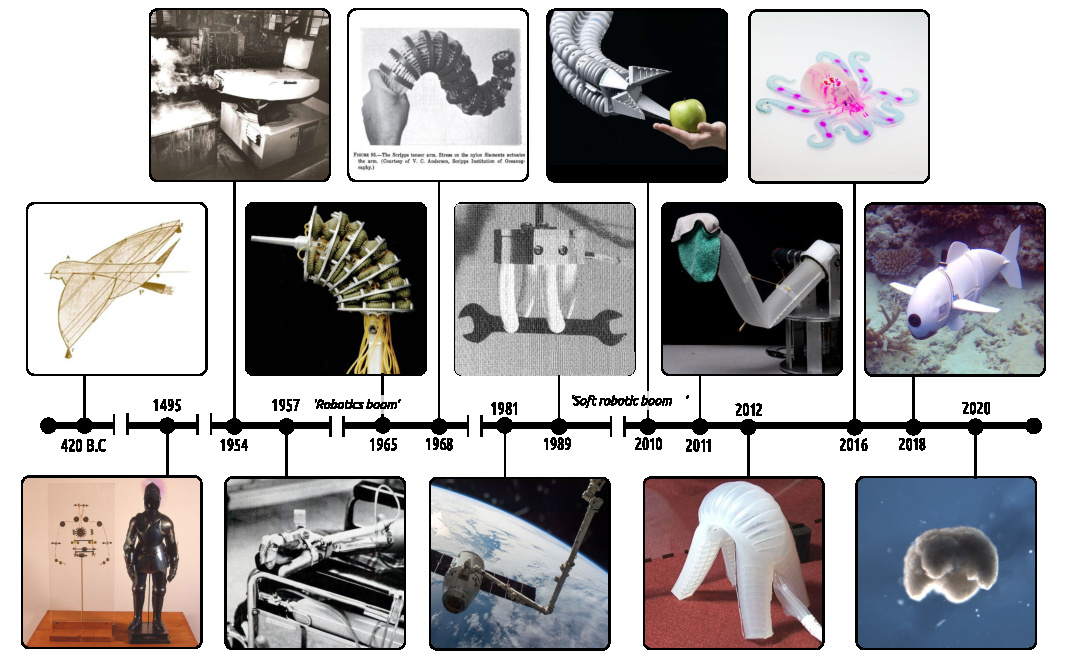
\includegraphics[width=1.11\textwidth]{./3_chapters/0_introduction/img/timeline_printer.pdf}
\fi
\caption{A brief timeline of the state-of-the-art of bio-inspired robotics throughout human history. {(1954):} Unimate, the first industrial robot . 
{(1957):} McKibben actuator, an early soft actuator inspired by the human muscle used for rehabilitation purposes \cite{Mckibben}. 
{(1965):} The Orm, believed to be the first soft robotic system designed by  Scheinman and Leifer \cite{BibEntryOrm2019Sep}. 
(1968): Tensor Scripps arm developed by Anderson \cite{Anderson1968}.
{(1981):} Canadarm-1, early flexible robotics employed on the International Space Station. 
{(1983):} Robot Arm with Pneumatic Gripper by Teleshev \cite{Teleshev1981}.
{(1984):} Bellows robotic arm by Wilson et al. \cite{Wilson2007}.
{(1989):} The soft robotic gripper developed by Suzumori et al. \cite{Suzumori1991,Suzumori1992}, seen as one of the earliest \textit{academic} soft robot, developed before the word \emph{soft robot} existed. 
{(2010):} Festo's Bionic arm inspired by the elephant's trunk \cite{Grzesiak2011}. 
{(2011):} Soft inflatable robot arm by Sanan and Atkeson \cite{Sanan2013,BibEntryBH62022Sep}.
(2012) Multi-gait soft robot capable of terrestial locomotion \cite{Choi2011}. 
(2016): Octobot, the first autonomous 3D-printed soft robot that explores a stabilizing oscillator chemical network that produces preprogrammed repetitive motion \cite{Wehner2016}.
(2018): Autonomous robotic fish made by Katzschmann \cite{Katzschmann2018}.
(2020): Xenobot, an organic soft robot composed of skin and muscle cells made by Blackiston and Kriegman \cite{Kriegman2019}.
}
\label{fig:C0:timeline}
\end{figure}
\clearpage
}

%\textbf{(Biomimicry in early automata)} One of the earliest examples of bio-mimicry is a mechanical wooden dove developed by mathematician Archytas of Tarentum in 350 BC. According to historians, the system was driven by compressed air or an internal steam-driven engine to achieve forward propulsion. It was believed to achieve traveling distances of ~200 \si{\meter} (see note\footnote{It was unclear if the devices was attached to a rope, or autonomous flight was achieved.}). Although might argue its lacks to sophistication to be considered a \emph{robot}, Archytas's invention could be considered as one of the earliest examples aviation, as its mechanical principles of achieving motion are undoubtedly similar to nowadays \emph{drone} technology. A millennium later, in the period of the High Renaissance, Leonardo da Vinci designed and constructed a mechanical knight around the 1490's -- and is thought to be the earliest robotic system. The mechanical constructions are perhaps closer to classical robots given our current perspective, and it was capable of various complex motions using preprogrammed sequences. 
%It is well-known that his work was built upon extensive anatomical research, which may have facilitated a deep understanding of the human body into the mechanical knight's robotic design. Given the work of Archytas and Da Vinci, biomimicry played a paramount role in the development of robot technologies before the term \emph{robot} was even introduced.

%\par In the 1920's, shortly after the second industrial revolution (1870 - 1914) and the first world war (1914), the first usage of the work \emph{robot} appeared -- originally meaning 'forced labor by serfs' (\ie, peasants) derived from the Czech word \emph{robota}. An common misconception is that robot implies slave, nonetheless, its origin is somewhat related. The word was popularized by Karel \v{C}apek in his play R.U.R. (Rossum’s Universal Robots) that involves an inventor named Rossum who discovers the secret of creating human-like machines. In his play, Rossom's robots assisted or fully alleviated mankind from any labor. Through human's ambition to assimilate man and machine, the robots ultimately gained the capacity for emotions. Shortly after, the robots, who were created to serve humans, have come to dominate mankind completely. The word \emph{robotics} was later solidified by Isaac Asimov, adapting the term from \v{C}apek. These works of science fiction are perhaps the fundamental groundwork of modern robotics which have led to the base practices of robotics and its corresponding academic field.

\textbf{Early soft actuation in robotics}. To relate the historical progress of soft robots to rigid robots, let us begin with early rigid robots. In 1954, George Devol filed a patent describing an autonomous robotic machine that could be preprogrammed to execute step-by-step motions \cite{Mickle2008}. The machine was designed to reduce the workload on the manufacturing work floor, with a major focus on mimicking repetitive (exhausting) human labor. In 1958, those prototypes led to a robotic system under the name \emph{Unimate}. An illustration of this early rigid robot is shown in Figure \ref{fig:C0:timeline}. The Unimate was used for manipulating metal die-casts and welding these to the main body of automobiles. In doing so revolutionizing the car industry shortly after. Much later (1969), Victor Scheinman created the Stanford Arm \cite{BibEntryStanford2022Sep,BibEntryOrm2019Sep}, recognized as the first electronic computer-controlled robotic arm because the Unimate's instructions (\ie, predefined setpoints in joint space) were prerecorded on a magnetic drum. He later developed the well-known PUMA robot in 1972 (video available at \cite{BibEntryPuma2022Sep}) -- the successor to the Unimate. Keep Scheinman in mind, as he ultimately ties to early soft robots. \vspace{0.085em}

\afterpage{
\begin{figure}[!t]
  %\hspace*{-1mm}
  \ifx\printFigures\undefined
  \else
  \centering
  %% This file was created by matlab2tikz.
%
%The latest updates can be retrieved from
%  http://www.mathworks.com/matlabcentral/fileexchange/22022-matlab2tikz-matlab2tikz
%where you can also make suggestions and rate matlab2tikz.
%
\definecolor{mycolor1}{rgb}{0.06275,0.35686,0.84706}%
\definecolor{mycolor2}{rgb}{0.86667,0.21176,0.10980}%
%
\begin{tikzpicture}

\begin{axis}[%
width=0.602\textwidth,
height=0.161\textwidth,
at={(0\textwidth,0.015\textwidth)},
scale only axis,
axis on top,
xmin=0.5,
xmax=2426.5,
tick align=outside,
y dir=reverse,
ymin=0.5,
ymax=650.5,
axis line style={draw=none},
ticks=none
]
\addplot [forget plot] graphics [xmin=0.5, xmax=2426.5, ymin=0.5, ymax=650.5] {fig_1_1-1.png};
\end{axis}

\begin{axis}[%
width=0.302\textwidth,
height=0.191\textwidth,
at={(0.648\textwidth,0\textwidth)},
scale only axis,
xmin=0,
xmax=1.5,
xlabel style={font=\color{white!15!black}},
xlabel={pressure (kPa)},
ymin=0,
ymax=35,
axis background/.style={fill=white},
xmajorgrids,
ymajorgrids,
legend style={at={(0.03,0.97)}, anchor=north west, legend columns=2, legend cell align=left, align=left, draw=white!15!black}
]
\addplot [color=mycolor1, line width=1.5pt]
  table[row sep=crcr]{%
0	0\\
0.00600149999999999	3.0568983103671\\
0.012003	5.35826739157104\\
0.024006	7.86017230302163\\
0.036009	9.05072762147565\\
0.0480119999999999	9.795136933107\\
0.0600149999999999	10.3164705929212\\
0.0720179999999999	10.711316657325\\
0.0840209999999999	11.0279129564825\\
0.0960239999999999	11.2925201532359\\
0.108027	11.5206742947192\\
0.1260315	11.8150953044601\\
0.144036	12.0694590939099\\
0.1620405	12.2959065095095\\
0.1860465	12.5672572998435\\
0.2100525	12.8138561366798\\
0.24006	13.0980192458931\\
0.276069	13.4149916949781\\
0.3180795	13.7633415653589\\
0.372093	14.1910487738014\\
0.456113999999999	14.8357726162343\\
0.588146999999999	15.8481229823956\\
0.660164999999999	16.4166289214781\\
0.726181499999999	16.9548047718235\\
0.786196499999999	17.4617841353458\\
0.840209999999999	17.9350495132933\\
0.894223499999999	18.4266813211065\\
0.948236999999999	18.9389704257632\\
0.996248999999999	19.413653689242\\
1.044261	19.9084481551956\\
1.092273	20.4253835409611\\
1.140285	20.9666992209241\\
1.1822955	21.4623032550621\\
1.224306	21.9803397018051\\
1.2663165	22.5228818415618\\
1.308327	23.0922527983715\\
1.3503375	23.6910711317645\\
1.392348	24.322306181775\\
1.43435850000001	24.9893459441392\\
1.47036750000001	25.5925254860443\\
1.4999985	26.11365092975\\
};
\addlegendentry{$\delta V$}

\addplot [color=mycolor2, line width=1.5pt]
  table[row sep=crcr]{%
0	0\\
0.00600149999999999	0.57694322540025\\
0.012003	1.8809393408942\\
0.0180045	2.95152432065056\\
0.024006	4.45583458122557\\
0.036009	6.19378149929854\\
0.0480119999999999	7.48539157943733\\
0.0600149999999999	8.4688855095399\\
0.0720179999999999	9.23690647886306\\
0.0840209999999999	9.85153659933535\\
0.0960239999999999	10.3531922792834\\
0.108027	10.7691384956111\\
0.12003	11.1184532554937\\
0.132033	11.4148904215117\\
0.144036	11.6686090629544\\
0.156039	11.8872685256996\\
0.168042	12.0767485361297\\
0.180045	12.2416363770546\\
0.192048	12.3855638977444\\
0.204051	12.511445089458\\
0.216054	12.6216464418373\\
0.228057	12.7181110468447\\
0.24006	12.8024503578201\\
0.252063	12.8760129819895\\
0.264066	12.9399369280069\\
0.276069	12.9951897701871\\
0.288072	13.0425998730449\\
0.300075	13.0828809209488\\
0.312078	13.1166513764424\\
0.324081	13.1444500557612\\
0.336084	13.1667487016037\\
0.348087	13.1839622118741\\
0.36009	13.1964570224759\\
0.372093	13.2045580243864\\
0.384096	13.2085543078992\\
0.3900975	13.2090949291082\\
};
\addlegendentry{$\delta\text{ \!\!L}$}

\addplot [color=mycolor2, dashed, line width=1.5pt, forget plot]
  table[row sep=crcr]{%
0.3900975	13.2090949291082\\
0.4021005	13.2074094834352\\
0.4141035	13.2022150575773\\
0.426106499999999	13.1937085356179\\
0.438109499999999	13.1820674082842\\
0.450112499999999	13.167452053111\\
0.462115499999999	13.1500076917316\\
0.480119999999999	13.1188216524309\\
0.498124499999999	13.0819593181423\\
0.516128999999999	13.0397643773147\\
0.534133499999999	12.9925364907466\\
0.552137999999999	12.940537547495\\
0.576143999999999	12.8641761270216\\
0.600149999999999	12.7802040746341\\
0.624155999999999	12.6890133020198\\
0.654163499999999	12.5653689878037\\
0.684170999999999	12.4314807991557\\
0.714178499999999	12.2877652488207\\
0.744185999999999	12.134547035545\\
0.780194999999999	11.9384837181762\\
0.816203999999999	11.7293863338915\\
0.852212999999999	11.5074325334682\\
0.888221999999999	11.2726938851784\\
0.924230999999999	11.0251466514001\\
0.960240000000001	10.7646794022534\\
1.0022505	10.4442081230322\\
1.044261	10.1054386868975\\
1.0862715	9.74777996411718\\
1.128282	9.3704926101939\\
1.1702925	8.97268281045118\\
1.212303	8.55329199813728\\
1.2543135	8.11108229372756\\
1.296324	7.64461717852633\\
1.3383345	7.15223665142942\\
1.380345	6.63202579865352\\
1.4223555	6.08177530074445\\
1.4583645	5.58429802632113\\
1.4943735	5.06103909220648\\
1.4999985	4.97621111560656\\
};
\end{axis}
\end{tikzpicture}%
  \fi
  \vspace{-3mm}
  \caption{Working principle of a basic pneumatic artificial muscle (\ie, Morin muscle \cite{Morin1953}) with the internal volume \data{Matlab1} in \si{\milli \liter}, and the end-effector displacement \data{Matlab2} in \si{\milli \meter} and \dashdata{Matlab2} is the point at which the undesirable ballooning occurs.
  \label{fig:C0:mckibben}}
\end{figure}

\begin{figure}[!t]
  \vspace{-0.6mm}
  \ifx\printFigures\undefined
  \else
  \centering
  %%!TEX root = ../../thesis.tex
%%%% CHAPTER 1 *****************************************************************
\chapter[Dynamic modeling of Soft Robots -- PCC case]{Dynamic modeling -- The Piece-wise Constant Approach}
\label{chap: chapter 1}

\blankfootnote{This chapter is based on:\\ .\disclaimer}

%%%% ABSTRACT ******************************************************************
\input{3_chapters/1_chapter/0_abstract.tex}

%%%% MAIN **********************************************************************
\section{Introduction} \label{sec: chap1 1_introduction}
\input{3_chapters/1_chapter/1_introduction.tex}

\newpage
\section{Continuum dynamic model}  \label{sec: chap2 section header}
\input{3_chapters/1_chapter/3_model.tex}

\newpage
\section{Extension to multi-link dynamics}  \label{sec: chap2 section header}
\input{3_chapters/1_chapter/4_multilink.tex}

\section{Efficient solver of the soft robotic dynamics through Matrix-Differential Equations}  \label{sec: chap2 section header}
\input{3_chapters/1_chapter/5_solver.tex}

%%%%%%%%%%%%%%%%%%%%%%%%%%%%%%%%%%%%%%%%%%%%%%%%%%%%%%%%%%%%%%%%%%%%%%%%%%%%%%%%

  %\input{/home/brandon/Documents/phd/thesis/3_chapters/0_introduction/img/PAM.pdf_tex}
  \fi
  \caption{Patent diagrams of pneumatic artificial muscle from 1953 till 1988. (a) Morin Muscle (1953, \cite{Morin1953}); (b) ROMAN muscle (1986, \cite{Immega1986}); (c) Yarlott muscle (1972, \cite{Yarlott1972}); (d) Kukolj muscle (1988, \cite{Kukolj1988}); (e) Paynter Hyperboloid (1974, \cite{Paynter1974}).
  \label{fig:C0:several_PAM}}
  \vspace{-5mm}
\end{figure}
}

Nearly four years after the Unimate was developed, Joseph L. McKibben developed a pneumatic muscle-inspired actuator capable of linear contraction -- called the McKibben actuator. The McKibben muscle is a type of Pneumatic Artificial Muscle (PAM) which is to this date the most frequently used and published artificial muscle in literature. According to \cite{Mckibben}, he developed the McKibben actuators to bring motion to his little daughter's polio-paralyzed hand. His aim was that eventually such pneumatic actuators may help patients with paralyzed fingers to move, grasp, and even write. Inspired by the human muscle, the McKibben actuator consists of an inflatable inner bladder enveloped with a double-helical weave. When pressurized, the fluidic actuator converts radial expansion into uni-axial contraction \cite{Daerden1999,Daerden2000,Schulte1961} since weave inhibits extensive \emph{ballooning} -- a term for undesired rapidly-accelerated volumetric expansion. Its material composition is often silicone rubber with a nylon-fiber exterior. A schematic representation of a general pneumatic muscle and the effect of ballooning are shown in Figure \ref{fig:C0:mckibben}. Ballooning is an (often undesired) nonlinear effect, where the hyper-elastic pressure vessel exhibits strain-softening after a critical point is reached. As a result, further increase of the pressure leads to an exponential growth in volume, which ultimately leads to actuator tearing. At stages of ballooning, mechanical performance significantly drops and even produces adverse effects, like actuation reversal. McKibben solved this problem through a combination of soft and inextensible fiber weaves. These inextensible were placed at the exterior wall of the soft muscle, thereby limiting the radial expansion before ballooning could occur. According to Daerden (1999, \cite{Daerden1999}), there exist many variations of pneumatic muscle besides braided muscles, such as the \emph{netted muscles} (e.g, Yarlott \cite{Yarlott1972}, ROMAC \cite{Immega1986}, and Kukolj \cite{Kukolj1988}) and \emph{embedded muscles} (\eg, Morin \cite{Morin1953}, Paynter Hyperboloid \cite{Paynter1988}). Illustration of their patent schematics are shown in Figure \ref{fig:C0:several_PAM}.

Pneumatic muscles are perhaps one of the first fundamental technologies that enabled soft robotics, and to this day, it remains a framework for many soft robotic systems. Nevertheless, besides the many examples of fluidics \cite{Marchese2014,Marchese2016,Katzschmann2018,Suzumori1991,Mosadegh2014}, there exist many other technologies employed in soft robotic motion: such as thermal \cite{Wu2021Dec} or chemical expansion/contraction \cite{Tolley2014,Bartlett2015,Wehner2016}, crystal re-alignment \cite{Pilz2020,Lopez2018,Vantomme2021,Polygerinos2013}, di-electric elastomers \cite{Keplinger2011}, magnetism \cite{Roh2019Apr,KimYoonho2018,McDonald2020,Boyvat2017Jul}, and naturally the use of tendons paired with electro-mechanical actuation \cite{Renda2018,Bern2019,Kim2020Jun,Coevoet2017Feb,Wang2016Sep}. Some predate the invention of the McKibben actuator. For example, a popular soft actuation principle still applied in soft robotics today are Dielectric Elastomer Actuators (DEA) developed by R\"{o}ntgen in 1880 \cite{Rontgen1880}. Therefore, given the abundance of soft robotic actuation, it is difficult to pinpoint the exact date of origin of soft actuation technology. Note, however, that these systems are not categorized as soft robots, they are categorized as soft actuators. Here, we emphasize the difference between soft actuators and soft robots in view of the modeling and control terminology relevant to the thesis:

\terminology{\textbf{Soft actuators} are controllable flexible actuation units of the constitute soft robot that through external stimuli are responsible for natural motion and/or change in adaptive compliance. %By definition, a soft actuator is a single-input-multi-output (SIMO) system.
}{}
%
\vspace{-4mm}
%
\begin{rmk} The terminology above attempts to address an ambiguity common to soft robotics, namely the interchangeable use of soft actuator and soft robot. The thesis invokes that soft robots must be comprised of multiple soft actuators that connect to a passive deformable body. Here, the soft body functions as a mechanical conduit between actuators, sensors, and the environment.
\end{rmk}
  %Let us also introduce the dual of soft actuators -- namely the \emph{soft sensor} that relate measurements to the motion of soft actuators:

\textbf{Origin of soft robotics}. Returning to 1965, nearly a decade after the invention of the McKibben actuator and the Unimate robot, Scheinman and Leifer proposed a novel pneumatic robotic arm named the \emph{Orm} -- Norwegian for snake (recall that he also developed the popular PUMA robot \cite{BibEntryPuma2022Sep}). The name was also an abbreviation for Object-Relational Mapping tool \cite{Corke2020}. To the author's knowledge, this is believed to be the first instance of a soft robotic system. Surprisingly the system predates any rigid snake-like robot, like the Scripps tensor arm by Anderson (1968, \cite{Anderson1968}). Inspired by the anatomy of snakes, the system featured 28 rubber pneumatic artificial muscle (\ie, bellows) distributed along a flexible backbone (\ie, skeletal support). The network of artificial muscles were sandwiched between steel plates to prevent misalignment. It is worth mentioning that the technology is analogous to the pneumatic McKibben muscle, where fiber weaves are used to prevent ballooning. Yet, contrary to a single McKibben actuator, the soft robotic system could undergo three-dimensional movement by inflation or deflation of an embedded pneumatic network. This led to a rich set of movements previously unseen in rigid robotics. As an illustrative example, we provided the mechanics of the Orm soft robot in Figure \ref{fig:C0:ormrobot}. The soft robot could achieve bending in any preferred direction by differential pressurization of each channel, and elongation through synchronized actuation. Most notably, comparing the volume-strain response of the Orm with respect to the McKibben actuator, \ie, comparing Figure \ref{fig:C0:mckibben} against \ref{fig:C0:ormrobot}, it is noticeably more linear in nature. Although not documented at the time, the comparison highlights the importance of structural geometry in pneumatic muscle networks.

\begin{figure}[!t]
  \ifx\printFigures\undefined
  \else
  \centering
  %% This file was created by matlab2tikz.
%
%The latest updates can be retrieved from
%  http://www.mathworks.com/matlabcentral/fileexchange/22022-matlab2tikz-matlab2tikz
%where you can also make suggestions and rate matlab2tikz.
%
\definecolor{mycolor1}{rgb}{0.06275,0.35686,0.84706}%
\definecolor{mycolor2}{rgb}{0.86667,0.21176,0.10980}%
%
\begin{tikzpicture}

\begin{axis}[%
width=0.583\textwidth,
height=0.214\textwidth,
at={(0\textwidth,0\textwidth)},
scale only axis,
axis on top,
xmin=0.5,
xmax=1768.5,
tick align=outside,
y dir=reverse,
ymin=0.5,
ymax=650.5,
axis line style={draw=none},
ticks=none
]
\addplot [forget plot] graphics [xmin=0.5, xmax=1768.5, ymin=0.5, ymax=650.5] {fig_orm_elong-1.png};
\end{axis}

\begin{axis}[%
width=0.308\textwidth,
height=0.195\textwidth,
at={(0.642\textwidth,0.01\textwidth)},
scale only axis,
xmin=0,
xmax=15,
ymin=0,
ymax=110,
axis background/.style={fill=white},
xmajorgrids,
ymajorgrids,
legend style={at={(0.03,0.97)}, anchor=north west, legend columns=2, legend cell align=left, align=left, draw=white!15!black}
]
\addplot [color=mycolor1, line width=1.5pt]
  table[row sep=crcr]{%
0	0\\
1.20005999999999	8.62875869322605\\
2.40012	17.0685830193392\\
3.60017999999999	25.3075020924564\\
4.80024	33.3362750448029\\
6.0003	41.1480614223673\\
7.20036	48.7381311097239\\
8.40042	56.1036109498542\\
9.60048	63.2432605846741\\
10.80054	70.1572704477627\\
11.700585	75.1955238137271\\
12.60063	80.1081200969719\\
13.500675	84.8973166125783\\
14.40072	89.5642639584667\\
15.00075	92.6047602820568\\
};
\addlegendentry{$\delta V$}

\addplot [color=mycolor2, line width=1.5pt]
  table[row sep=crcr]{%
0	0\\
1.500075	9.4713120804718\\
3.00015	18.7367798341987\\
4.20021	25.9889383302985\\
5.40027000000001	33.0912743243296\\
6.60033	40.0387557751286\\
7.80039000000001	46.8277828635893\\
9.00045	53.4559850403998\\
10.20051	59.922055247927\\
11.40057	66.2256106025044\\
12.60063	72.3665219327312\\
13.80069	78.346840194486\\
15.00075	84.1642843326511\\
};
\addlegendentry{$\delta L$}

\end{axis}

\begin{axis}[%
width=1.08\textwidth,
height=0.244\textwidth,
at={(-0.022\textwidth,-0.015\textwidth)},
scale only axis,
xmin=0,
xmax=1,
ymin=0,
ymax=1,
axis line style={draw=none},
ticks=none,
axis x line*=bottom,
axis y line*=left
]
\end{axis}
\end{tikzpicture}%
  %% This file was created by matlab2tikz.
%
%The latest updates can be retrieved from
%  http://www.mathworks.com/matlabcentral/fileexchange/22022-matlab2tikz-matlab2tikz
%where you can also make suggestions and rate matlab2tikz.
%
\definecolor{mycolor1}{rgb}{0.06275,0.35686,0.84706}%
\definecolor{mycolor2}{rgb}{1.0000,0.6157,0.1176}%
%
\begin{tikzpicture}

\begin{axis}[%
width=0.583\textwidth,
height=0.186\textwidth,
at={(0\textwidth,0.005\textwidth)},
scale only axis,
axis on top,
xmin=0.5,
xmax=2037.5,
tick align=outside,
y dir=reverse,
ymin=0.5,
ymax=650.5,
axis line style={draw=none},
ticks=none
]
\addplot [forget plot] graphics [xmin=0.5, xmax=2037.5, ymin=0.5, ymax=650.5] {./fig/fig_orm_bend-1.png};
\end{axis}

\begin{axis}[%
width=0.308\textwidth,
height=0.195\textwidth,
at={(0.642\textwidth,0\textwidth)},
scale only axis,
xmin=0,
xmax=30,
xlabel style={font=\color{white!15!black}},
xlabel={pressure (kPa)},
ymin=0,
ymax=110,
axis background/.style={fill=white},
xmajorgrids,
ymajorgrids,
legend style={at={(0.03,0.97)}, anchor=north west, legend columns=2, legend cell align=left, align=left, draw=white!15!black}
]
\addplot [color=mycolor1, line width=1.5pt]
  table[row sep=crcr]{%
0	0\\
1.60008	2.43048322137711\\
4.0002	6.19782561266756\\
4.80024	7.46829805994749\\
5.60028	8.34214292028537\\
17.60088	25.9279210387424\\
18.40092	27.0804871808147\\
19.20096	27.8807159907824\\
20.001	29.291815814346\\
20.80104	30.1255987953186\\
21.60108	31.5485305130109\\
22.40112	32.3659198775631\\
24.0012	34.5026095847334\\
28.80144	41.0337024135815\\
30.40152	43.1793137664006\\
};
\addlegendentry{$\delta V$}

\addplot [color=mycolor2, line width=1.5pt]
  table[row sep=crcr]{%
0	0\\
3.20016	8.88556718870406\\
6.40032000000001	17.5260854409956\\
8.80043999999999	23.7584681055126\\
11.20056	29.7734109354827\\
13.60068	35.566935673684\\
16.0008	41.1374336291155\\
17.60088	44.7277626743178\\
20.001	50.0250200383298\\
20.80104	51.6388516477443\\
21.60108	53.3837573512613\\
22.40112	54.9453731417261\\
23.20116	56.644891426995\\
24.80124	59.8364150546849\\
26.40132	62.9180842306127\\
28.0014	65.909936141282\\
29.60148	68.8150689926074\\
30.40152	70.2358435840924\\
};
\addlegendentry{$\theta$}

\end{axis}

\begin{axis}[%
width=1.08\textwidth,
height=0.244\textwidth,
at={(-0.022\textwidth,-0.024\textwidth)},
scale only axis,
xmin=0,
xmax=1,
ymin=0,
ymax=1,
axis line style={draw=none},
ticks=none,
axis x line*=bottom,
axis y line*=left
]
\end{axis}
\end{tikzpicture}%
  \vspace{-6mm}
  \fi
  
  \caption{Working principle of the Orm robotic manipulator \cite{BibEntryOrm2019Sep} with the internal volume \data{Matlab1} in \si{\milli \liter}, and the end-effector displacement \data{Matlab2} in \si{\milli \meter} and bending-angle \data{Matlab4} in deg. By actuation of the pneumatic network, both elongation and bending can be achieved. Observe that the response is significantly more linear than McKibben actuators in Fig. \ref{fig:C0:mckibben}, emphasizing the importance of geometry.
  %\dotdata{Matlab2}
  \vspace{-6mm}
  \label{fig:C0:ormrobot}}
\end{figure}

According to an interview with Scheinman led by Asaro et al. \cite{ETHW2020Dec} in 2010, the positional accuracy of the system was poor, yet the concepts of pneumatically-driven soft arms continued for many years. The positional inaccuracy of pneumatic soft actuators at the time may have caused its lost of academic interest in the 60's. Three years later, in 1968, an improved hyper-redundant robot manipulator was proposed and patented by Anderson and Horn \cite{Anderson1968} (see Figure \ref{fig:C0:timeline}). Improving upon the Orm, which was deemed slow and had limited positional accuracy, Anderson proposed an array of nylon tendons that were connected to rigid discs distributed along the redundant backbone of the robot. The configurable backbone was comprised of universal spherical joints that allow for pivoting motion with respect to other discs -- totalling 16 Degrees-of-Freedom (DOFs). The entire arm was actuated hydraulically, yet the (soft) actuators were placed outside the robot's body rather than placed at each joint, like the Orm. To improve positional accuracy further, Anderson placed sensor tendons parallel the actuator tendons which allowed for operator-based positional feedback. Although Anderson's robot does not categorize as a soft robot since it relies mostly on rigid materials, its flexibility arose from thin nylon tendons that were used for both actuation and sensing. Anderson showed that a network of distributed sensors are necessary to control the complex morphological shapes in  hyper-redundant robotic systems, while also mitigating the sensor's effect on mobility. Within this context, let us define soft sensors:

\terminology{\textbf{(Proprioceptive) soft sensors} are flexible measurements units embedded into the soft robotic body that through external stimuli measure the (local) changes of the system. Softness here implies that the sensor minimally alters the global mechanical behavior of the robot. %By definition, a soft sensor is a multi-input-single-output (MISO) system.
}{}
%
\begin{rmk}
  \vspace{-1mm}
As the emphasize lies on "minimally alters the global mechanical behavior", soft sensors may be composed of stiff (perhaps even rigid) components. Our definition infers that these sensors must be placed into or onto the soft body, minimally affecting the operational workspace of the soft actuator network in static or dynamic condition.
\end{rmk}

\textbf{Soft robotics in the 80's}. Following the fundamental works of McKibben, Scheinman and Anderson, the field of soft Pneumatic Artificial Muscles (PAMs) in robotics evolved rapidly in the early 80's. A few soft robotic systems are shown in Figure \ref{fig:C0:earlyPAMrobots}. Teleshev (1981, \cite{Teleshev1981}) developed a soft gripper reminiscent of modern PneuNet actuators \cite{Galloway2016,Mosadegh2014,Choi2011} -- a rectangular bellow-shaped soft actuator. Unlike uniaxial PAMs, which are radially symmetric, these soft grippers explored an asymmetrical design of bellows. The geometry led to a stiffness differential around the circumference, resulting in their icon bending motion. Still popular today, these pneumatic bending actuators find their origin back in early 1974, see Andorf et al. (1974, \cite{Andorf1974}). A decade later, Takagi et al. (\cite{Takagi1983}, 1983) developed a soft multi-joint robot manipulator that resembles the human arm with its movements and antagonistic muscle pairs. Although, their PAMs -- called \textit{Rubbertuator} -- had a function and design identical to McKibben's PAMs, their system showed the merits of combining soft and rigid. They observed not only a high-degree of positional control of the robot arm, force control was easily regulated by the pressure control. This naturally had safety benefits. The soft robot arm could perform delicate low-force tasks while simultaneously blocking motion when encountering a human. These (soft) properties were lacking in rigid robotic manipulators at the time but reminiscent in its biological counterpart -- the human arm. Note that, at that time, force and impedance control for rigid robotics had been topics of academic research for years \cite{Anderson1988,Khatib1987,Hogan1984,Hogan1984Jan}, dating back to the early 1970's. (\eg, see also \cite{Markiewicz1973}). Yet achieving similar properties without control were rarely explored at the time.
%
\begin{figure}[!t]
  \vspace{-2mm}
  \ifx\printFigures\undefined
  \else
  \hspace{1mm}
  % This file was created by matlab2tikz.
%
%The latest updates can be retrieved from
%  http://www.mathworks.com/matlabcentral/fileexchange/22022-matlab2tikz-matlab2tikz
%where you can also make suggestions and rate matlab2tikz.
%
\begin{tikzpicture}

\begin{axis}[%
width=0.95\textwidth,
height=0.238\textwidth,
at={(0\textwidth,0\textwidth)},
scale only axis,
axis on top,
clip=false,
xmin=0.5,
xmax=2593.5,
tick align=outside,
y dir=reverse,
ymin=0.5,
ymax=650.5,
axis line style={draw=none},
ticks=none,
axis x line*=bottom,
axis y line*=left
]
\addplot [forget plot] graphics [xmin=0.5, xmax=2593.5, ymin=0.5, ymax=650.5] {./fig/fig_earlyPAMrobots-1.png};
\node[right, align=left]
at (axis cs:203,780) {\small (a)};
\node[right, align=left]
at (axis cs:777.5,780) {\small (b)};
\node[right, align=left]
at (axis cs:1326,780) {\small (c)};
\node[right, align=left]
at (axis cs:1801,780) {\small (d)};
\node[right, align=left]
at (axis cs:2226,780) {\small (e)};
\end{axis}
\end{tikzpicture}%
  \fi
  %\vspace{-2mm}
  \caption{Early robotic systems that explored soft PAMs for various tasks. (a) Soft robotic grippers by Teleshev (1981, \cite{Teleshev1981}). (b) The soft arm using \textit{Rubbertuator} actuators by Takagi and Sakaguchi (1983, \cite{Takagi1983}). (c) Three-link soft robotic manipulator with gripper reminiscent of the elephant's trunk, developed by Wilson at Duke University (1984, \cite{Wilson2007,Weisburd1988}). (d) Shadow bipedal walker by Buckley et al. (1988, \cite{Buckley2012}) using McKibben muscle in antagonistic pairs to produce locomotion.
  \label{fig:C0:earlyPAMrobots}}
  \vspace{-2mm}
\end{figure}
%
\par Shortly after, Wilson (1984, \cite{Wilson2007}) developed a soft robot manipulator based on the elephant's trunk at Duke University, Durham. His design effectively combined the works of Teleshev \cite{Teleshev1981} and Takagi et al. \cite{Takagi1983} into a robot with similar dexterity but minimal use of rigid components. According to \cite{Weisburd1988}, his idea stemmed from the work of Kier and Smith (1985, \cite{Kier1985}) who studied the biomechanics of muscular-hydrostats in animals, like cephalopods (\eg, squids). The work of Kier et al. \cite{Kier1985} studied how complex motions are produces in muscular organs, like elongation, shortening, bending and torsion. Inspired by the muscular hydrostat in the elephant's trunk, Wilson developed a soft arm composed of polyurethane tubes that work as half-bellows, which enabled expansion and bending under positive pressurization \cite{Weisburd1988}. To accommodate for three-dimensional movement, each soft pneumatic link was placed at a $ \phi = \frac{\pi}{2}$ twist offset w.r.t. to the previous link. To illustrate the motion of the soft arm, a few snapshots are provided in Figure \ref{fig:C0:fist_srm_robot}. Wilson hypothesized that these highly-complaint robots will be more mechanically robust and be sufficiently dexterous for tight workspaces, contrary to its rigid counterparts. Although the dexterity was novel, the positional accuracy was poor. The main problem stemmed from the soft arm being controlled in open-loop (\ie, remote tele-operation) without proprioceptive sensing nor any positional feedback control. An issue akin to the Orm (1965). 

A few years later, Buckley et al. (1988, \cite{Buckley2012}) developed the Shadow walker -- a bipedal rigid robot comprised of antagonistic McKibben muscle pairs. Although not fully soft, their system did explore proprioceptive sensing. The hip, knee, and ankle joints were equipped with resistance-variable potentiometers for position feedback, whereas all the muscles had tension sensors for force feedback. Later on, these resistive sensors were replaced by analog optical sensors to improve robustness \cite{Buckley2012}. Although the system was top-heavy, due to the pneumatic control hardware (\eg, valves and piping), rudimentary locomotion was possible. Interestingly, a similar artificial muscle system is still explored in nowadays humanoid robotics, like the Atlas from Boston Dynamics. The success of pairing soft muscles with proprioceptive sensing eventually led to the development of the McKibben Shadow hand \cite{Buckley2012,Gong2022Feb}, comprised of 40 uniquely addressable soft muscles. 

\begin{figure}[!t]
  \vspace{-2mm}
  \ifx\printFigures\undefined
  \else
  \centering
  % This file was created by matlab2tikz.
%
%The latest updates can be retrieved from
%  http://www.mathworks.com/matlabcentral/fileexchange/22022-matlab2tikz-matlab2tikz
%where you can also make suggestions and rate matlab2tikz.
%
\begin{tikzpicture}

\begin{axis}[%
width=0.712\textwidth,
height=0.295\textwidth,
at={(0.11\textwidth,0.03\textwidth)},
scale only axis,
xmin=0,
xmax=1,
ymin=0,
ymax=1,
axis line style={draw=none},
ticks=none,
axis x line*=bottom,
axis y line*=left
]
\end{axis}

\begin{axis}[%
width=0.218\textwidth,
height=0.164\textwidth,
at={(0\textwidth,0.179\textwidth)},
scale only axis,
axis on top,
xmin=0.5,
xmax=480.5,
tick align=outside,
y dir=reverse,
ymin=0.5,
ymax=360.5,
axis line style={draw=none},
ticks=none
]
\addplot [forget plot] graphics [xmin=0.5, xmax=480.5, ymin=0.5, ymax=360.5] {fig_first_srm-1.png};
\node[right, align=left, font=\color{white}]
at (axis cs:15,320) {\scriptsize $t = 0$ s};
\end{axis}

\begin{axis}[%
width=0.218\textwidth,
height=0.164\textwidth,
at={(0.227\textwidth,0.179\textwidth)},
scale only axis,
axis on top,
xmin=0.5,
xmax=480.5,
tick align=outside,
y dir=reverse,
ymin=0.5,
ymax=360.5,
axis line style={draw=none},
ticks=none
]
\addplot [forget plot] graphics [xmin=0.5, xmax=480.5, ymin=0.5, ymax=360.5] {fig_first_srm-2.png};
\node[right, align=left, font=\color{white}]
at (axis cs:15,320) {\scriptsize $t = 1.9$ s};
\end{axis}

\begin{axis}[%
width=0.218\textwidth,
height=0.164\textwidth,
at={(0.455\textwidth,0.179\textwidth)},
scale only axis,
axis on top,
xmin=0.5,
xmax=480.5,
tick align=outside,
y dir=reverse,
ymin=0.5,
ymax=360.5,
axis line style={draw=none},
ticks=none
]
\addplot [forget plot] graphics [xmin=0.5, xmax=480.5, ymin=0.5, ymax=360.5] {fig_first_srm-3.png};
\node[right, align=left, font=\color{white}]
at (axis cs:15,320) {\scriptsize $t = 2.8$ s};
\end{axis}

\begin{axis}[%
width=0.218\textwidth,
height=0.164\textwidth,
at={(0.682\textwidth,0.179\textwidth)},
scale only axis,
axis on top,
xmin=0.5,
xmax=480.5,
tick align=outside,
y dir=reverse,
ymin=0.5,
ymax=360.5,
axis line style={draw=none},
ticks=none
]
\addplot [forget plot] graphics [xmin=0.5, xmax=480.5, ymin=0.5, ymax=360.5] {fig_first_srm-4.png};
\node[right, align=left, font=\color{white}]
at (axis cs:15,320) {\scriptsize $t = 5.6$ s};
\end{axis}

\begin{axis}[%
width=0.218\textwidth,
height=0.164\textwidth,
at={(0\textwidth,0\textwidth)},
scale only axis,
axis on top,
xmin=0.5,
xmax=480.5,
tick align=outside,
y dir=reverse,
ymin=0.5,
ymax=360.5,
axis line style={draw=none},
ticks=none
]
\addplot [forget plot] graphics [xmin=0.5, xmax=480.5, ymin=0.5, ymax=360.5] {fig_first_srm-5.png};
\node[right, align=left, font=\color{white}]
at (axis cs:15,320) {\scriptsize $t = 6.5$ s};
\end{axis}

\begin{axis}[%
width=0.218\textwidth,
height=0.164\textwidth,
at={(0.227\textwidth,0\textwidth)},
scale only axis,
axis on top,
xmin=0.5,
xmax=480.5,
tick align=outside,
y dir=reverse,
ymin=0.5,
ymax=360.5,
axis line style={draw=none},
ticks=none
]
\addplot [forget plot] graphics [xmin=0.5, xmax=480.5, ymin=0.5, ymax=360.5] {fig_first_srm-6.png};
\node[right, align=left, font=\color{white}]
at (axis cs:15,320) {\scriptsize $t = 9.3$ s};
\end{axis}

\begin{axis}[%
width=0.218\textwidth,
height=0.164\textwidth,
at={(0.455\textwidth,0\textwidth)},
scale only axis,
axis on top,
xmin=0.5,
xmax=480.5,
tick align=outside,
y dir=reverse,
ymin=0.5,
ymax=360.5,
axis line style={draw=none},
ticks=none
]
\addplot [forget plot] graphics [xmin=0.5, xmax=480.5, ymin=0.5, ymax=360.5] {fig_first_srm-7.png};
\node[right, align=left, font=\color{white}]
at (axis cs:15,320) {\scriptsize $t = 10$ s};
\end{axis}

\begin{axis}[%
width=0.218\textwidth,
height=0.164\textwidth,
at={(0.682\textwidth,0\textwidth)},
scale only axis,
axis on top,
xmin=0.5,
xmax=480.5,
tick align=outside,
y dir=reverse,
ymin=0.5,
ymax=360.5,
axis line style={draw=none},
ticks=none
]
\addplot [forget plot] graphics [xmin=0.5, xmax=480.5, ymin=0.5, ymax=360.5] {fig_first_srm-8.png};
\node[right, align=left, font=\color{white}]
at (axis cs:15,320) {\scriptsize $t = 14$ s};
\end{axis}
\end{tikzpicture}%
  \fi
  %\vspace{-2mm}
  \caption{Three-link soft robotic manipulator with two-fingered soft gripper by James Wilson from Stanford university (1984, \cite{Wilson2007}). Unlike classic manipulators, where links and joints are separated, Wilson's robot consisted of three pneumatic bending actuators -- being link and joint simultaneously. 
  \vspace{-4mm}
  \label{fig:C0:fist_srm_robot}}
\end{figure}

\begin{figure}[!t]
  \vspace{-3mm}
  \ifx\printFigures\undefined
  \else
  \centering
  % This file was created by matlab2tikz.
%
%The latest updates can be retrieved from
%  http://www.mathworks.com/matlabcentral/fileexchange/22022-matlab2tikz-matlab2tikz
%where you can also make suggestions and rate matlab2tikz.
%
\begin{tikzpicture}

\begin{axis}[%
width=0.712\textwidth,
height=0.295\textwidth,
at={(0.11\textwidth,0.032\textwidth)},
scale only axis,
xmin=0,
xmax=1,
ymin=0,
ymax=1,
axis line style={draw=none},
ticks=none,
axis x line*=bottom,
axis y line*=left
]
\end{axis}

\begin{axis}[%
width=0.218\textwidth,
height=0.168\textwidth,
at={(0\textwidth,0.179\textwidth)},
scale only axis,
axis on top,
xmin=0.5,
xmax=302.5,
tick align=outside,
y dir=reverse,
ymin=0.5,
ymax=233.5,
axis line style={draw=none},
ticks=none
]
\addplot [forget plot] graphics [xmin=0.5, xmax=302.5, ymin=0.5, ymax=233.5] {fig_first_gripper-1.png};
\node[right, align=left, font=\color{white}]
at (axis cs:7,209) {\scriptsize $t = 0$ s};
\end{axis}

\begin{axis}[%
width=0.218\textwidth,
height=0.168\textwidth,
at={(0.227\textwidth,0.179\textwidth)},
scale only axis,
axis on top,
xmin=0.5,
xmax=302.5,
tick align=outside,
y dir=reverse,
ymin=0.5,
ymax=233.5,
axis line style={draw=none},
ticks=none
]
\addplot [forget plot] graphics [xmin=0.5, xmax=302.5, ymin=0.5, ymax=233.5] {fig_first_gripper-2.png};
\node[right, align=left, font=\color{white}]
at (axis cs:7,209) {\scriptsize $t = 0.14$ s};
\end{axis}

\begin{axis}[%
width=0.218\textwidth,
height=0.168\textwidth,
at={(0.455\textwidth,0.179\textwidth)},
scale only axis,
axis on top,
xmin=0.5,
xmax=302.5,
tick align=outside,
y dir=reverse,
ymin=0.5,
ymax=233.5,
axis line style={draw=none},
ticks=none
]
\addplot [forget plot] graphics [xmin=0.5, xmax=302.5, ymin=0.5, ymax=233.5] {fig_first_gripper-3.png};
\node[right, align=left, font=\color{white}]
at (axis cs:7,209) {\scriptsize $t = 0.28$ s};
\end{axis}

\begin{axis}[%
width=0.218\textwidth,
height=0.168\textwidth,
at={(0.682\textwidth,0.179\textwidth)},
scale only axis,
axis on top,
xmin=0.5,
xmax=302.5,
tick align=outside,
y dir=reverse,
ymin=0.5,
ymax=233.5,
axis line style={draw=none},
ticks=none
]
\addplot [forget plot] graphics [xmin=0.5, xmax=302.5, ymin=0.5, ymax=233.5] {fig_first_gripper-4.png};
\node[right, align=left, font=\color{white}]
at (axis cs:7,209) {\scriptsize $t = 0.55$ s};
\end{axis}

\begin{axis}[%
width=0.218\textwidth,
height=0.168\textwidth,
at={(0\textwidth,0\textwidth)},
scale only axis,
axis on top,
xmin=0.5,
xmax=302.5,
tick align=outside,
y dir=reverse,
ymin=0.5,
ymax=233.5,
axis line style={draw=none},
ticks=none
]
\addplot [forget plot] graphics [xmin=0.5, xmax=302.5, ymin=0.5, ymax=233.5] {fig_first_gripper-5.png};
\node[right, align=left, font=\color{white}]
at (axis cs:7,209) {\scriptsize $t = 0.69$ s};
\end{axis}

\begin{axis}[%
width=0.218\textwidth,
height=0.168\textwidth,
at={(0.227\textwidth,0\textwidth)},
scale only axis,
axis on top,
xmin=0.5,
xmax=302.5,
tick align=outside,
y dir=reverse,
ymin=0.5,
ymax=233.5,
axis line style={draw=none},
ticks=none
]
\addplot [forget plot] graphics [xmin=0.5, xmax=302.5, ymin=0.5, ymax=233.5] {fig_first_gripper-6.png};
\node[right, align=left, font=\color{white}]
at (axis cs:7,209) {\scriptsize $t = 0.83$ s};
\end{axis}

\begin{axis}[%
width=0.218\textwidth,
height=0.168\textwidth,
at={(0.455\textwidth,0\textwidth)},
scale only axis,
axis on top,
xmin=0.5,
xmax=302.5,
tick align=outside,
y dir=reverse,
ymin=0.5,
ymax=233.5,
axis line style={draw=none},
ticks=none
]
\addplot [forget plot] graphics [xmin=0.5, xmax=302.5, ymin=0.5, ymax=233.5] {fig_first_gripper-7.png};
\node[right, align=left, font=\color{white}]
at (axis cs:7,209) {\scriptsize $t = 0.97$ s};
\end{axis}

\begin{axis}[%
width=0.218\textwidth,
height=0.168\textwidth,
at={(0.682\textwidth,0\textwidth)},
scale only axis,
axis on top,
xmin=0.5,
xmax=302.5,
tick align=outside,
y dir=reverse,
ymin=0.5,
ymax=233.5,
axis line style={draw=none},
ticks=none
]
\addplot [forget plot] graphics [xmin=0.5, xmax=302.5, ymin=0.5, ymax=233.5] {fig_first_gripper-8.png};
\node[right, align=left, font=\color{white}]
at (axis cs:7,209) {\scriptsize $t = 1.2$ s};
\end{axis}
\end{tikzpicture}%
  \fi
  %\vspace{-2mm}
  \caption{Four-fingered soft robotic gripper by Suzumori and Saiko (1989, \cite{Suzumori1991,Suzumori1992}). Each finger possess three pneumatic chambers that allow for directional bending -- analogous the Orm. Through proper coordination of the set of soft fingers various gripping complexity can be achieved, such as the clock-wise turning a mechanical hex bolt (as shown above). Suzumori et al. showed these intricate finger motions can be easily achieved by careful modeling of the fingertip dynamics, and exploring the adaptability of soft materials.
  \label{fig:C0:fist_grip_robot}}
  \vspace{-3mm}
\end{figure}

Following, Suzumori and Saiko (1989, \cite{Suzumori1991,Suzumori1992}) developed a micro flexible soft actuator driven by an electro-hydraulic system (intrinsic length $L \approx12$ \si{\milli \meter}). Each end-effector enables three DOFs including pitch, yaw, and stretch -- making it ideal for fingers, arms and legs. Figure \ref{fig:C0:fist_grip_robot} shows the level of dexterity in their system. By placing the four PAMs parallel on a gripper mount, and assigning a pre-defined trajectory, they showed their soft robotic system has sufficient dexterity to mount an hex-bolt at an incredible speed and precision. To achieve such dexterity and precision, Suzumori et al. \cite{Suzumori1991} employed various modeling and control strategies to account for the dynamical characteristics under high-frequency, fluid compressibility, and the closing mechanics of pressure valves. Futhermore, the kinematics of each finger was derived using generalized homogenous transformation, not unlike traditional robotics. Knowing both the compliance characteristics (pressure-deformation relations) and the forward kinematics, a Jacobian-based positional controller was employed to regulate the Cartesian coordinates of the finger-tips (successfully one might add).
%
\par \textbf{Early controllers for hyper-redundant (soft) robots}. Following the increasing interest in highly-flexible robots around the late 80's, academic research into controlling these \textit{hyper-redundant} robots boomed shortly after. At the time, the term hyper-redundancy -- being an extension to redundancy in robotics \cite{MerriamWebster1983} -- was defined as the relative degree of kinematic and/or actuator redundancy which is large or even infinite \cite{Chirikjian1992,Chirikjian1994}. The term was first introduced by Chirikjian and Burdick (1989, \cite{Chirikjian1989}). Others referred to these robots as \textit{highly redundant} \cite{Wilson1988Dec,Naccarato1989Dec} or \textit{High Degree-of-Freedom} (HDOF) manipulator \cite{Salerno1989Jan,Mochiyama1999}. Around that time, Chirikjian and Burdick provided a plenary of mathematical foundation \cite{Chirikjian1994,Chirikjian1994Jun,Chirikjian1991,Chirikjian1992,Chirikjian1992Dec} focussed on the kinematics and motion planning of hyper-redundant manipulators. Their work presented a modal discretization approach to describe the shape of the deformable backbone \cite{Chirikjian1994Jun}, and from this geometric approaches were introduced to solve obstacle avoiding trajectories using generalized \textit{follow-the-leader} strategies \cite{Chirikjian1992Dec}. Especially the latter showed the limitation in rigid redundant manipulators. Although Chirikjian laid the foundation for the control of hyper-redundant robot, basic principles of motion planning in pneumatic hyper-redundant robots were already presented by Wilson et al. (1988, \cite{Wilson1988Dec,Wilson1989Jun}) -- yet were not called hyper-redundant robots nor soft robots yet. Recall also that the work of Wilson et al. has been sown earlier in Figure \ref{fig:C0:timeline} and Figure \ref{fig:C0:fist_srm_robot}. In Brock et al. (1991, \cite{Brock1991}), a similar analysis was used for optimal shape design of thin elastic rods to realize desired robotic compliance. Besides, there exist an abundance of literature prior to \cite{Chirikjian1992} on Variable Geometry Truss Manipulators (VGTMs) -- a variant of hyper-redundant tensegrity robotics -- that dealt with motion planning for such systems \cite{Naccarato1989Dec,Naccarato1991Apr,Salerno1989Jan}. Later, Mochiyama et al. \cite{Mochiyama1998,Mochiyama1999}, built upon Chirikjian's work by extending it to a dynamic formulation for elastic rods such that classic controller design is possible. They proposed shape-regulation controllers for HDOF manipulator by projecting them onto time-invariant curves, thereby showing that the estimation the desired curve parameters is the crucial key to solving the problem by Lyapunov design \cite{Mochiyama1998}. Although there existed a variety of modeling and control strategies, computational power in relation to modeling complexity was the limiting factor for the simulation-to-reality transfer at the time.

%\subsection{REF}
% \begin{itemize}
%   \item . F. Shulte, "The Characteristics of the Mckibben Artificial Muscle", The Application of External Power in Prosthetics and Orthetics, pp. 94-115, 1960.
%   \item A. Chen, R. Yin, L. Cao, C. Yuan, H. K. Ding and W. J. Zhang, "Soft robotics: Definition and research issues," 2017 24th International Conference on Mechatronics and Machine Vision in Practice (M2VIP), 2017, pp. 366-370, doi: 10.1109/M2VIP.2017.8267170.

\vspace{-4mm}
\section{Challenges in modern soft robotics}
\label{sec:C0:1.2}
%
\begin{figure}[!t]
  \vspace{-2mm}
  \ifx\printFigures\undefined
  \else
  \centering
  \vspace{-2mm}
  % This file was created by matlab2tikz.
%
%The latest updates can be retrieved from
%  http://www.mathworks.com/matlabcentral/fileexchange/22022-matlab2tikz-matlab2tikz
%where you can also make suggestions and rate matlab2tikz.
%
\definecolor{mycolor1}{rgb}{0.06275,0.35686,0.84706}%
\definecolor{mycolor2}{rgb}{0.86667,0.21176,0.10980}%
\definecolor{mycolor3}{rgb}{0.18039,0.52157,0.25098}%
\definecolor{mycolor4}{rgb}{1.00000,0.30980,0.00000}%
%
\begin{tikzpicture}

\begin{axis}[%
width=0.866\textwidth,
height=0.318\textwidth,
at={(0\textwidth,0\textwidth)},
scale only axis,
xmin=723181,
xmax=739618,
xtick={723181,725008,726834,728660,730486,732313,734139,735965,737791,739618},
xticklabels={{1980},{1985},{1990},{1995},{2000},{2005},{2010},{2015},{2020},{2025}},
scaled x ticks=false,
ymin=-1000,
ymax=25000,
ylabel style={font=\color{white!15!black}},
ylabel={\#publications (cumulative)},
axis background/.style={fill=white},
xmajorgrids,
ymajorgrids,
legend style={at={(0.03,0.97)}, anchor=north west, legend cell align=left, align=left, draw=white!15!black}
]
\addplot [color=mycolor1, line width=2.0pt, only marks, mark size=1.7pt, mark=*, mark options={solid, mycolor1}]
  table[row sep=crcr]{%
729756	31\\
730121	75\\
730486	125\\
730852	187\\
731217	247\\
731582	327\\
731947	425\\
732313	557\\
732678	675\\
733043	825\\
733408	980\\
733774	1140\\
734139	1318\\
734504	1471\\
734869	1732\\
735235	2039\\
735600	2458\\
735965	2984\\
736330	3680\\
736696	4681\\
737061	6027\\
737426	7816\\
737791	9942\\
738157	12408\\
738522	13791\\
};
\addlegendentry{Soft robot(s)}

\addplot [color=mycolor2, line width=2.0pt, only marks, mark size=1.1pt, mark=square, mark options={solid, mycolor2}]
  table[row sep=crcr]{%
723547	4\\
724277	12\\
724642	19\\
725008	34\\
725373	43\\
725738	58\\
726103	66\\
726469	117\\
726834	168\\
727199	275\\
727564	423\\
727930	582\\
728295	737\\
728660	899\\
729025	1163\\
729391	1423\\
729756	1714\\
730121	1907\\
730486	2109\\
730852	2343\\
731217	2563\\
731582	2818\\
731947	3084\\
732313	3390\\
732678	3741\\
733043	4116\\
733408	4557\\
733774	5007\\
734139	5482\\
734504	5936\\
734869	6529\\
735235	7133\\
735600	7826\\
735965	8563\\
736330	9482\\
736696	10586\\
737061	11827\\
737426	13342\\
737791	14847\\
738157	16584\\
738522	17555\\
};
\addlegendentry{Flexible/redundant robot(s)}

\addplot [color=mycolor3, line width=2.0pt, only marks, mark size=1.7pt, mark=diamond, mark options={solid, mycolor3}]
  table[row sep=crcr]{%
727199	1\\
727564	2\\
727930	4\\
728295	9\\
728660	12\\
729025	28\\
729391	55\\
729756	81\\
730121	118\\
730486	153\\
730852	190\\
731217	240\\
731582	294\\
731947	365\\
732313	439\\
732678	533\\
733043	662\\
733408	783\\
733774	894\\
734139	1050\\
734504	1179\\
734869	1375\\
735235	1584\\
735600	1864\\
735965	2175\\
736330	2612\\
736696	3218\\
737061	4031\\
737426	5109\\
737791	6243\\
738157	7542\\
738522	8281\\
};
\addlegendentry{Soft actuator(s)}

\addplot [color=mycolor4, dashed, line width=1.5pt]
  table[row sep=crcr]{%
728660	44.6634216554798\\
728660	44.6634216554798\\
728660	44.6634216554798\\
728660	44.6634216554798\\
728660	44.6634216554798\\
728660	44.6634216554798\\
728660	44.6634216554798\\
728660	44.6634216554798\\
728660	44.6634216554798\\
728660	44.6634216554798\\
728660	44.6634216554798\\
728660	44.6634216554798\\
728660	44.6634216554798\\
728660	44.6634216554798\\
728660	44.6634216554798\\
728660	44.6634216554798\\
728660	44.6634216554798\\
729025	53.3890888278004\\
729025	53.3890888278004\\
729025	53.3890888278004\\
729025	53.3890888278004\\
729025	53.3890888278004\\
729025	53.3890888278004\\
729025	53.3890888278004\\
729025	53.3890888278004\\
729025	53.3890888278004\\
729025	53.3890888278004\\
729025	53.3890888278004\\
729025	53.3890888278004\\
729025	53.3890888278004\\
729025	53.3890888278004\\
729025	53.3890888278004\\
729025	53.3890888278004\\
729025	53.3890888278004\\
729025	53.3890888278004\\
729025	53.3890888278004\\
729025	53.3890888278004\\
729025	53.3890888278004\\
729025	53.3890888278004\\
729025	53.3890888278004\\
729025	53.3890888278004\\
729025	53.3890888278004\\
729025	53.3890888278004\\
729025	53.3890888278004\\
729025	53.3890888278004\\
729025	53.3890888278004\\
729025	53.3890888278004\\
729025	53.3890888278004\\
729025	53.3890888278004\\
729025	53.3890888278004\\
729391	64.3112289380452\\
729391	64.3112289380452\\
729391	64.3112289380452\\
729391	64.3112289380452\\
729391	64.3112289380452\\
729391	64.3112289380452\\
729391	64.3112289380452\\
729391	64.3112289380452\\
729391	64.3112289380452\\
729391	64.3112289380452\\
729391	64.3112289380452\\
729391	64.3112289380452\\
729391	64.3112289380452\\
729391	64.3112289380452\\
729391	64.3112289380452\\
729391	64.3112289380452\\
729391	64.3112289380452\\
729391	64.3112289380452\\
729391	64.3112289380452\\
729391	64.3112289380452\\
729391	64.3112289380452\\
729391	64.3112289380452\\
729391	64.3112289380452\\
729391	64.3112289380452\\
729391	64.3112289380452\\
729391	64.3112289380452\\
729391	64.3112289380452\\
729391	64.3112289380452\\
729391	64.3112289380452\\
729391	64.3112289380452\\
729391	64.3112289380452\\
729391	64.3112289380452\\
729391	64.3112289380452\\
729391	64.3112289380452\\
729756	77.9827502362947\\
729756	77.9827502362947\\
729756	77.9827502362947\\
729756	77.9827502362947\\
729756	77.9827502362947\\
729756	77.9827502362947\\
729756	77.9827502362947\\
729756	77.9827502362947\\
729756	77.9827502362947\\
729756	77.9827502362947\\
729756	77.9827502362947\\
729756	77.9827502362947\\
729756	77.9827502362947\\
729756	77.9827502362947\\
729756	77.9827502362947\\
729756	77.9827502362947\\
729756	77.9827502362947\\
729756	77.9827502362947\\
729756	77.9827502362947\\
729756	77.9827502362947\\
729756	77.9827502362947\\
729756	77.9827502362947\\
729756	77.9827502362947\\
729756	77.9827502362947\\
729756	77.9827502362947\\
729756	77.9827502362947\\
729756	77.9827502362947\\
729756	77.9827502362947\\
729756	77.9827502362947\\
729756	77.9827502362947\\
729756	77.9827502362947\\
729756	77.9827502362947\\
729756	77.9827502362947\\
730121	95.095742078724\\
730121	95.095742078724\\
730121	95.095742078724\\
730121	95.095742078724\\
730121	95.095742078724\\
730121	95.095742078724\\
730121	95.095742078724\\
730121	95.095742078724\\
730121	95.095742078724\\
730121	95.095742078724\\
730121	95.095742078724\\
730121	95.095742078724\\
730121	95.095742078724\\
730121	95.095742078724\\
730121	95.095742078724\\
730121	95.095742078724\\
730121	95.095742078724\\
730121	95.095742078724\\
730121	95.095742078724\\
730121	95.095742078724\\
730121	95.095742078724\\
730121	95.095742078724\\
730121	95.095742078724\\
730121	95.095742078724\\
730121	95.095742078724\\
730121	95.095742078724\\
730121	95.095742078724\\
730121	95.095742078724\\
730121	95.095742078724\\
730121	95.095742078724\\
730121	95.095742078724\\
730121	95.095742078724\\
730121	95.095742078724\\
730486	116.516510361223\\
730486	116.516510361223\\
730486	116.516510361223\\
730486	116.516510361223\\
730486	116.516510361223\\
730486	116.516510361223\\
730486	116.516510361223\\
730486	116.516510361223\\
730486	116.516510361223\\
730486	116.516510361223\\
730486	116.516510361223\\
730486	116.516510361223\\
730486	116.516510361223\\
730486	116.516510361223\\
730486	116.516510361223\\
730486	116.516510361223\\
730486	116.516510361223\\
730486	116.516510361223\\
730486	116.516510361223\\
730486	116.516510361223\\
730486	116.516510361223\\
730486	116.516510361223\\
730486	116.516510361223\\
730486	116.516510361223\\
730486	116.516510361223\\
730486	116.516510361223\\
730486	116.516510361223\\
730486	116.516510361223\\
730486	116.516510361223\\
730486	116.516510361223\\
730486	116.516510361223\\
730486	116.516510361223\\
730486	116.516510361223\\
730486	116.516510361223\\
730852	143.329432265087\\
730852	143.329432265087\\
730852	143.329432265087\\
730852	143.329432265087\\
730852	143.329432265087\\
730852	143.329432265087\\
730852	143.329432265087\\
730852	143.329432265087\\
730852	143.329432265087\\
730852	143.329432265087\\
730852	143.329432265087\\
730852	143.329432265087\\
730852	143.329432265087\\
730852	143.329432265087\\
730852	143.329432265087\\
730852	143.329432265087\\
730852	143.329432265087\\
730852	143.329432265087\\
730852	143.329432265087\\
730852	143.329432265087\\
730852	143.329432265087\\
730852	143.329432265087\\
730852	143.329432265087\\
730852	143.329432265087\\
730852	143.329432265087\\
730852	143.329432265087\\
730852	143.329432265087\\
730852	143.329432265087\\
730852	143.329432265087\\
730852	143.329432265087\\
730852	143.329432265087\\
730852	143.329432265087\\
730852	143.329432265087\\
731217	176.891850360523\\
731217	176.891850360523\\
731217	176.891850360523\\
731217	176.891850360523\\
731217	176.891850360523\\
731217	176.891850360523\\
731217	176.891850360523\\
731217	176.891850360523\\
731217	176.891850360523\\
731217	176.891850360523\\
731217	176.891850360523\\
731217	176.891850360523\\
731217	176.891850360523\\
731217	176.891850360523\\
731217	176.891850360523\\
731217	176.891850360523\\
731217	176.891850360523\\
731217	176.891850360523\\
731217	176.891850360523\\
731217	176.891850360523\\
731217	176.891850360523\\
731217	176.891850360523\\
731217	176.891850360523\\
731217	176.891850360523\\
731217	176.891850360523\\
731217	176.891850360523\\
731217	176.891850360523\\
731217	176.891850360523\\
731217	176.891850360523\\
731217	176.891850360523\\
731217	176.891850360523\\
731217	176.891850360523\\
731217	176.891850360523\\
731582	218.902784955852\\
731582	218.902784955852\\
731582	218.902784955852\\
731582	218.902784955852\\
731582	218.902784955852\\
731582	218.902784955852\\
731582	218.902784955852\\
731582	218.902784955852\\
731582	218.902784955852\\
731582	218.902784955852\\
731582	218.902784955852\\
731582	218.902784955852\\
731582	218.902784955852\\
731582	218.902784955852\\
731582	218.902784955852\\
731582	218.902784955852\\
731582	218.902784955852\\
731582	218.902784955852\\
731582	218.902784955852\\
731582	218.902784955852\\
731582	218.902784955852\\
731582	218.902784955852\\
731582	218.902784955852\\
731582	218.902784955852\\
731582	218.902784955852\\
731582	218.902784955852\\
731582	218.902784955852\\
731582	218.902784955852\\
731582	218.902784955852\\
731582	218.902784955852\\
731582	218.902784955852\\
731582	218.902784955852\\
731582	218.902784955852\\
731582	218.902784955852\\
731947	271.48894309721\\
731947	271.48894309721\\
731947	271.48894309721\\
731947	271.48894309721\\
731947	271.48894309721\\
731947	271.48894309721\\
731947	271.48894309721\\
731947	271.48894309721\\
731947	271.48894309721\\
731947	271.48894309721\\
731947	271.48894309721\\
731947	271.48894309721\\
731947	271.48894309721\\
731947	271.48894309721\\
731947	271.48894309721\\
731947	271.48894309721\\
731947	271.48894309721\\
731947	271.48894309721\\
731947	271.48894309721\\
731947	271.48894309721\\
731947	271.48894309721\\
731947	271.48894309721\\
731947	271.48894309721\\
731947	271.48894309721\\
731947	271.48894309721\\
731947	271.48894309721\\
731947	271.48894309721\\
731947	271.48894309721\\
731947	271.48894309721\\
731947	271.48894309721\\
731947	271.48894309721\\
731947	271.48894309721\\
731947	271.48894309721\\
732313	337.312378226773\\
732313	337.312378226773\\
732313	337.312378226773\\
732313	337.312378226773\\
732313	337.312378226773\\
732313	337.312378226773\\
732313	337.312378226773\\
732313	337.312378226773\\
732313	337.312378226773\\
732313	337.312378226773\\
732313	337.312378226773\\
732313	337.312378226773\\
732313	337.312378226773\\
732313	337.312378226773\\
732313	337.312378226773\\
732313	337.312378226773\\
732313	337.312378226773\\
732313	337.312378226773\\
732313	337.312378226773\\
732313	337.312378226773\\
732313	337.312378226773\\
732313	337.312378226773\\
732313	337.312378226773\\
732313	337.312378226773\\
732313	337.312378226773\\
732313	337.312378226773\\
732313	337.312378226773\\
732313	337.312378226773\\
732313	337.312378226773\\
732313	337.312378226773\\
732313	337.312378226773\\
732313	337.312378226773\\
732313	337.312378226773\\
732678	419.705250522346\\
732678	419.705250522346\\
732678	419.705250522346\\
732678	419.705250522346\\
732678	419.705250522346\\
732678	419.705250522346\\
732678	419.705250522346\\
732678	419.705250522346\\
732678	419.705250522346\\
732678	419.705250522346\\
732678	419.705250522346\\
732678	419.705250522346\\
732678	419.705250522346\\
732678	419.705250522346\\
732678	419.705250522346\\
732678	419.705250522346\\
732678	419.705250522346\\
732678	419.705250522346\\
732678	419.705250522346\\
732678	419.705250522346\\
732678	419.705250522346\\
732678	419.705250522346\\
732678	419.705250522346\\
732678	419.705250522346\\
732678	419.705250522346\\
732678	419.705250522346\\
732678	419.705250522346\\
732678	419.705250522346\\
732678	419.705250522346\\
732678	419.705250522346\\
732678	419.705250522346\\
732678	419.705250522346\\
732678	419.705250522346\\
733043	522.838509850919\\
733043	522.838509850919\\
733043	522.838509850919\\
733043	522.838509850919\\
733043	522.838509850919\\
733043	522.838509850919\\
733043	522.838509850919\\
733043	522.838509850919\\
733043	522.838509850919\\
733043	522.838509850919\\
733043	522.838509850919\\
733043	522.838509850919\\
733043	522.838509850919\\
733043	522.838509850919\\
733043	522.838509850919\\
733043	522.838509850919\\
733043	522.838509850919\\
733043	522.838509850919\\
733043	522.838509850919\\
733043	522.838509850919\\
733043	522.838509850919\\
733043	522.838509850919\\
733043	522.838509850919\\
733043	522.838509850919\\
733043	522.838509850919\\
733043	522.838509850919\\
733043	522.838509850919\\
733043	522.838509850919\\
733043	522.838509850919\\
733043	522.838509850919\\
733043	522.838509850919\\
733043	522.838509850919\\
733043	522.838509850919\\
733043	522.838509850919\\
733408	651.933040523155\\
733408	651.933040523155\\
733408	651.933040523155\\
733408	651.933040523155\\
733408	651.933040523155\\
733408	651.933040523155\\
733408	651.933040523155\\
733408	651.933040523155\\
733408	651.933040523155\\
733408	651.933040523155\\
733408	651.933040523155\\
733408	651.933040523155\\
733408	651.933040523155\\
733408	651.933040523155\\
733408	651.933040523155\\
733408	651.933040523155\\
733408	651.933040523155\\
733408	651.933040523155\\
733408	651.933040523155\\
733408	651.933040523155\\
733408	651.933040523155\\
733408	651.933040523155\\
733408	651.933040523155\\
733408	651.933040523155\\
733408	651.933040523155\\
733408	651.933040523155\\
733408	651.933040523155\\
733408	651.933040523155\\
733408	651.933040523155\\
733408	651.933040523155\\
733408	651.933040523155\\
733408	651.933040523155\\
733408	651.933040523155\\
733774	813.523956566939\\
733774	813.523956566939\\
733774	813.523956566939\\
733774	813.523956566939\\
733774	813.523956566939\\
733774	813.523956566939\\
733774	813.523956566939\\
733774	813.523956566939\\
733774	813.523956566939\\
733774	813.523956566939\\
733774	813.523956566939\\
733774	813.523956566939\\
733774	813.523956566939\\
733774	813.523956566939\\
733774	813.523956566939\\
733774	813.523956566939\\
733774	813.523956566939\\
733774	813.523956566939\\
733774	813.523956566939\\
733774	813.523956566939\\
733774	813.523956566939\\
733774	813.523956566939\\
733774	813.523956566939\\
733774	813.523956566939\\
733774	813.523956566939\\
733774	813.523956566939\\
733774	813.523956566939\\
733774	813.523956566939\\
733774	813.523956566939\\
733774	813.523956566939\\
733774	813.523956566939\\
733774	813.523956566939\\
733774	813.523956566939\\
734139	1015.79142686097\\
734139	1015.79142686097\\
734139	1015.79142686097\\
734139	1015.79142686097\\
734139	1015.79142686097\\
734139	1015.79142686097\\
734139	1015.79142686097\\
734139	1015.79142686097\\
734139	1015.79142686097\\
734139	1015.79142686097\\
734139	1015.79142686097\\
734139	1015.79142686097\\
734139	1015.79142686097\\
734139	1015.79142686097\\
734139	1015.79142686097\\
734139	1015.79142686097\\
734139	1015.79142686097\\
734139	1015.79142686097\\
734139	1015.79142686097\\
734139	1015.79142686097\\
734139	1015.79142686097\\
734139	1015.79142686097\\
734139	1015.79142686097\\
734139	1015.79142686097\\
734139	1015.79142686097\\
734139	1015.79142686097\\
734139	1015.79142686097\\
734139	1015.79142686097\\
734139	1015.79142686097\\
734139	1015.79142686097\\
734139	1015.79142686097\\
734139	1015.79142686097\\
734139	1015.79142686097\\
734139	1015.79142686097\\
734504	1268.97477739086\\
734504	1268.97477739086\\
734504	1268.97477739086\\
734504	1268.97477739086\\
734504	1268.97477739086\\
734504	1268.97477739086\\
734504	1268.97477739086\\
734504	1268.97477739086\\
734504	1268.97477739086\\
734504	1268.97477739086\\
734504	1268.97477739086\\
734504	1268.97477739086\\
734504	1268.97477739086\\
734504	1268.97477739086\\
734504	1268.97477739086\\
734504	1268.97477739086\\
734504	1268.97477739086\\
734504	1268.97477739086\\
734504	1268.97477739086\\
734504	1268.97477739086\\
734504	1268.97477739086\\
734504	1268.97477739086\\
734504	1268.97477739086\\
734504	1268.97477739086\\
734504	1268.97477739086\\
734504	1268.97477739086\\
734504	1268.97477739086\\
734504	1268.97477739086\\
734504	1268.97477739086\\
734504	1268.97477739086\\
734504	1268.97477739086\\
734504	1268.97477739086\\
734504	1268.97477739086\\
734869	1585.89083360259\\
734869	1585.89083360259\\
734869	1585.89083360259\\
734869	1585.89083360259\\
734869	1585.89083360259\\
734869	1585.89083360259\\
734869	1585.89083360259\\
734869	1585.89083360259\\
734869	1585.89083360259\\
734869	1585.89083360259\\
734869	1585.89083360259\\
734869	1585.89083360259\\
734869	1585.89083360259\\
734869	1585.89083360259\\
734869	1585.89083360259\\
734869	1585.89083360259\\
734869	1585.89083360259\\
734869	1585.89083360259\\
734869	1585.89083360259\\
734869	1585.89083360259\\
734869	1585.89083360259\\
734869	1585.89083360259\\
734869	1585.89083360259\\
734869	1585.89083360259\\
734869	1585.89083360259\\
734869	1585.89083360259\\
734869	1585.89083360259\\
734869	1585.89083360259\\
734869	1585.89083360259\\
734869	1585.89083360259\\
734869	1585.89083360259\\
734869	1585.89083360259\\
734869	1585.89083360259\\
735235	1982.58274274519\\
735235	1982.58274274519\\
735235	1982.58274274519\\
735235	1982.58274274519\\
735235	1982.58274274519\\
735235	1982.58274274519\\
735235	1982.58274274519\\
735235	1982.58274274519\\
735235	1982.58274274519\\
735235	1982.58274274519\\
735235	1982.58274274519\\
735235	1982.58274274519\\
735235	1982.58274274519\\
735235	1982.58274274519\\
735235	1982.58274274519\\
735235	1982.58274274519\\
735235	1982.58274274519\\
735235	1982.58274274519\\
735235	1982.58274274519\\
735235	1982.58274274519\\
735235	1982.58274274519\\
735235	1982.58274274519\\
735235	1982.58274274519\\
735235	1982.58274274519\\
735235	1982.58274274519\\
735235	1982.58274274519\\
735235	1982.58274274519\\
735235	1982.58274274519\\
735235	1982.58274274519\\
735235	1982.58274274519\\
735235	1982.58274274519\\
735235	1982.58274274519\\
735235	1982.58274274519\\
735235	1982.58274274519\\
735600	2479.13212134172\\
735600	2479.13212134172\\
735600	2479.13212134172\\
735600	2479.13212134172\\
735600	2479.13212134172\\
735600	2479.13212134172\\
735600	2479.13212134172\\
735600	2479.13212134172\\
735600	2479.13212134172\\
735600	2479.13212134172\\
735600	2479.13212134172\\
735600	2479.13212134172\\
735600	2479.13212134172\\
735600	2479.13212134172\\
735600	2479.13212134172\\
735600	2479.13212134172\\
735600	2479.13212134172\\
735600	2479.13212134172\\
735600	2479.13212134172\\
735600	2479.13212134172\\
735600	2479.13212134172\\
735600	2479.13212134172\\
735600	2479.13212134172\\
735600	2479.13212134172\\
735600	2479.13212134172\\
735600	2479.13212134172\\
735600	2479.13212134172\\
735600	2479.13212134172\\
735600	2479.13212134172\\
735600	2479.13212134172\\
735600	2479.13212134172\\
735600	2479.13212134172\\
735600	2479.13212134172\\
735965	3100.67564088946\\
735965	3100.67564088946\\
735965	3100.67564088946\\
735965	3100.67564088946\\
735965	3100.67564088946\\
735965	3100.67564088946\\
735965	3100.67564088946\\
735965	3100.67564088946\\
735965	3100.67564088946\\
735965	3100.67564088946\\
735965	3100.67564088946\\
735965	3100.67564088946\\
735965	3100.67564088946\\
735965	3100.67564088946\\
735965	3100.67564088946\\
735965	3100.67564088946\\
735965	3100.67564088946\\
735965	3100.67564088946\\
735965	3100.67564088946\\
735965	3100.67564088946\\
735965	3100.67564088946\\
735965	3100.67564088946\\
735965	3100.67564088946\\
735965	3100.67564088946\\
735965	3100.67564088946\\
735965	3100.67564088946\\
735965	3100.67564088946\\
735965	3100.67564088946\\
735965	3100.67564088946\\
735965	3100.67564088946\\
735965	3100.67564088946\\
735965	3100.67564088946\\
735965	3100.67564088946\\
736330	3878.67751410433\\
736330	3878.67751410433\\
736330	3878.67751410433\\
736330	3878.67751410433\\
736330	3878.67751410433\\
736330	3878.67751410433\\
736330	3878.67751410433\\
736330	3878.67751410433\\
736330	3878.67751410433\\
736330	3878.67751410433\\
736330	3878.67751410433\\
736330	3878.67751410433\\
736330	3878.67751410433\\
736330	3878.67751410433\\
736330	3878.67751410433\\
736330	3878.67751410433\\
736330	3878.67751410433\\
736330	3878.67751410433\\
736330	3878.67751410433\\
736330	3878.67751410433\\
736330	3878.67751410433\\
736330	3878.67751410433\\
736330	3878.67751410433\\
736330	3878.67751410433\\
736330	3878.67751410433\\
736330	3878.67751410433\\
736330	3878.67751410433\\
736330	3878.67751410433\\
736330	3878.67751410433\\
736330	3878.67751410433\\
736330	3878.67751410433\\
736330	3878.67751410433\\
736330	3878.67751410433\\
736696	4852.52229840244\\
736696	4852.52229840244\\
736696	4852.52229840244\\
736696	4852.52229840244\\
736696	4852.52229840244\\
736696	4852.52229840244\\
736696	4852.52229840244\\
736696	4852.52229840244\\
736696	4852.52229840244\\
736696	4852.52229840244\\
736696	4852.52229840244\\
736696	4852.52229840244\\
736696	4852.52229840244\\
736696	4852.52229840244\\
736696	4852.52229840244\\
736696	4852.52229840244\\
736696	4852.52229840244\\
736696	4852.52229840244\\
736696	4852.52229840244\\
736696	4852.52229840244\\
736696	4852.52229840244\\
736696	4852.52229840244\\
736696	4852.52229840244\\
736696	4852.52229840244\\
736696	4852.52229840244\\
736696	4852.52229840244\\
736696	4852.52229840244\\
736696	4852.52229840244\\
736696	4852.52229840244\\
736696	4852.52229840244\\
736696	4852.52229840244\\
736696	4852.52229840244\\
736696	4852.52229840244\\
736696	4852.52229840244\\
737061	6071.50864863545\\
737061	6071.50864863545\\
737061	6071.50864863545\\
737061	6071.50864863545\\
737061	6071.50864863545\\
737061	6071.50864863545\\
737061	6071.50864863545\\
737061	6071.50864863545\\
737061	6071.50864863545\\
737061	6071.50864863545\\
737061	6071.50864863545\\
737061	6071.50864863545\\
737061	6071.50864863545\\
737061	6071.50864863545\\
737061	6071.50864863545\\
737061	6071.50864863545\\
737061	6071.50864863545\\
737061	6071.50864863545\\
737061	6071.50864863545\\
737061	6071.50864863545\\
737061	6071.50864863545\\
737061	6071.50864863545\\
737061	6071.50864863545\\
737061	6071.50864863545\\
737061	6071.50864863545\\
737061	6071.50864863545\\
737061	6071.50864863545\\
737061	6071.50864863545\\
737061	6071.50864863545\\
737061	6071.50864863545\\
737061	6071.50864863545\\
737061	6071.50864863545\\
737061	6071.50864863545\\
737426	7597.34494823154\\
737426	7597.34494823154\\
737426	7597.34494823154\\
737426	7597.34494823154\\
737426	7597.34494823154\\
737426	7597.34494823154\\
737426	7597.34494823154\\
737426	7597.34494823154\\
737426	7597.34494823154\\
737426	7597.34494823154\\
737426	7597.34494823154\\
737426	7597.34494823154\\
737426	7597.34494823154\\
737426	7597.34494823154\\
737426	7597.34494823154\\
737426	7597.34494823154\\
737426	7597.34494823154\\
737426	7597.34494823154\\
737426	7597.34494823154\\
737426	7597.34494823154\\
737426	7597.34494823154\\
737426	7597.34494823154\\
737426	7597.34494823154\\
737426	7597.34494823154\\
737426	7597.34494823154\\
737426	7597.34494823154\\
737426	7597.34494823154\\
737426	7597.34494823154\\
737426	7597.34494823154\\
737426	7597.34494823154\\
737426	7597.34494823154\\
737426	7597.34494823154\\
737426	7597.34494823154\\
737791	9507.27315433496\\
737791	9507.27315433496\\
737791	9507.27315433496\\
737791	9507.27315433496\\
737791	9507.27315433496\\
737791	9507.27315433496\\
737791	9507.27315433496\\
737791	9507.27315433496\\
737791	9507.27315433496\\
737791	9507.27315433496\\
737791	9507.27315433496\\
737791	9507.27315433496\\
737791	9507.27315433496\\
737791	9507.27315433496\\
737791	9507.27315433496\\
737791	9507.27315433496\\
737791	9507.27315433496\\
737791	9507.27315433496\\
737791	9507.27315433496\\
737791	9507.27315433496\\
737791	9507.27315433496\\
737791	9507.27315433496\\
737791	9507.27315433496\\
737791	9507.27315433496\\
737791	9507.27315433496\\
737791	9507.27315433496\\
737791	9507.27315433496\\
737791	9507.27315433496\\
737791	9507.27315433496\\
737791	9507.27315433496\\
737791	9507.27315433496\\
737791	9507.27315433496\\
737791	9507.27315433496\\
737791	9507.27315433496\\
738157	11897.9789944274\\
738157	11897.9789944274\\
738157	11897.9789944274\\
738157	11897.9789944274\\
738157	11897.9789944274\\
738157	11897.9789944274\\
738157	11897.9789944274\\
738157	11897.9789944274\\
738157	11897.9789944274\\
738157	11897.9789944274\\
738157	11897.9789944274\\
738157	11897.9789944274\\
738157	11897.9789944274\\
738157	11897.9789944274\\
738157	11897.9789944274\\
738157	11897.9789944274\\
738157	11897.9789944274\\
738157	11897.9789944274\\
738157	11897.9789944274\\
738157	11897.9789944274\\
738157	11897.9789944274\\
738157	11897.9789944274\\
738157	11897.9789944274\\
738157	11897.9789944274\\
738157	11897.9789944274\\
738157	11897.9789944274\\
738157	11897.9789944274\\
738157	11897.9789944274\\
738157	11897.9789944274\\
738157	11897.9789944274\\
738157	11897.9789944274\\
738157	11897.9789944274\\
738157	11897.9789944274\\
738522	14890.4864591518\\
738522	14890.4864591518\\
738522	14890.4864591518\\
738522	14890.4864591518\\
738522	14890.4864591518\\
738522	14890.4864591518\\
738522	14890.4864591518\\
738522	14890.4864591518\\
738522	14890.4864591518\\
738522	14890.4864591518\\
738522	14890.4864591518\\
738522	14890.4864591518\\
738522	14890.4864591518\\
738522	14890.4864591518\\
738522	14890.4864591518\\
738522	14890.4864591518\\
738522	14890.4864591518\\
738522	14890.4864591518\\
738522	14890.4864591518\\
738522	14890.4864591518\\
738522	14890.4864591518\\
738522	14890.4864591518\\
738522	14890.4864591518\\
738522	14890.4864591518\\
738522	14890.4864591518\\
738522	14890.4864591518\\
738522	14890.4864591518\\
738522	14890.4864591518\\
738522	14890.4864591518\\
738522	14890.4864591518\\
738522	14890.4864591518\\
738522	14890.4864591518\\
738522	14890.4864591518\\
738887	18636.2843637928\\
738887	18636.2843637928\\
738887	18636.2843637928\\
738887	18636.2843637928\\
738887	18636.2843637928\\
738887	18636.2843637928\\
738887	18636.2843637928\\
738887	18636.2843637928\\
738887	18636.2843637928\\
738887	18636.2843637928\\
738887	18636.2843637928\\
738887	18636.2843637928\\
738887	18636.2843637928\\
738887	18636.2843637928\\
738887	18636.2843637928\\
738887	18636.2843637928\\
738887	18636.2843637928\\
738887	18636.2843637928\\
738887	18636.2843637928\\
738887	18636.2843637928\\
738887	18636.2843637928\\
738887	18636.2843637928\\
738887	18636.2843637928\\
738887	18636.2843637928\\
738887	18636.2843637928\\
738887	18636.2843637928\\
738887	18636.2843637928\\
738887	18636.2843637928\\
738887	18636.2843637928\\
738887	18636.2843637928\\
738887	18636.2843637928\\
738887	18636.2843637928\\
738887	18636.2843637928\\
738887	18636.2843637928\\
739252	23324.9951215135\\
739252	23324.9951215135\\
739252	23324.9951215135\\
739252	23324.9951215135\\
739252	23324.9951215135\\
739252	23324.9951215135\\
739252	23324.9951215135\\
739252	23324.9951215135\\
739252	23324.9951215135\\
739252	23324.9951215135\\
739252	23324.9951215135\\
739252	23324.9951215135\\
739252	23324.9951215135\\
739252	23324.9951215135\\
739252	23324.9951215135\\
739252	23324.9951215135\\
739252	23324.9951215135\\
739252	23324.9951215135\\
739252	23324.9951215135\\
739252	23324.9951215135\\
739252	23324.9951215135\\
739252	23324.9951215135\\
739252	23324.9951215135\\
739252	23324.9951215135\\
739252	23324.9951215135\\
739252	23324.9951215135\\
739252	23324.9951215135\\
739252	23324.9951215135\\
739252	23324.9951215135\\
739252	23324.9951215135\\
739252	23324.9951215135\\
739252	23324.9951215135\\
739252	23324.9951215135\\
739618	29193.9739423751\\
739618	29193.9739423751\\
739618	29193.9739423751\\
739618	29193.9739423751\\
739618	29193.9739423751\\
739618	29193.9739423751\\
739618	29193.9739423751\\
739618	29193.9739423751\\
739618	29193.9739423751\\
739618	29193.9739423751\\
739618	29193.9739423751\\
739618	29193.9739423751\\
739618	29193.9739423751\\
739618	29193.9739423751\\
739618	29193.9739423751\\
739618	29193.9739423751\\
739618	29193.9739423751\\
};
\addlegendentry{Prediction}

\end{axis}
\end{tikzpicture}%
  \fi
  \vspace{-1mm}
  \caption{Cumulative number of (scientific) publications on the topic of \emph{soft robots} or related topics. Data acquired from the Web of Sciences data repository.}
  \vspace{-3mm}
  \label{fig:C0:publicationhistory}
\end{figure}
%
The exact date of the academic boom of soft robotics is unclear, but it is believed to be the mid 2000's. To motivate the argument, we have provided a graph of scientific publications on the topic \textit{soft robot(s)} from 1980 till 2022 (see Figure \ref{fig:C0:publicationhistory}). It shows the cumulative number of publications related to the term soft robot in the titles, keywords, and abstracts. The publication data from Figure \ref{fig:C0:publicationhistory} is obtained using the Web of Sciences data repository. Let it be clear that the term \textit{soft robot} was introduced decades after hyper-redundant robots, thus some older academic work might be lost simply due to different terminology. Hence, we also provided related topics such as '\textit{flexible}' and '\textit{redundant robot(s)}'. In the following section, we will discuss modern trends and challenges in the field of soft robotics, that continue the research paths of highly-flexible robots in early 90's.

\begin{rmk}In retrospect to the previous section, soft robotics is an extensive and diverse academic field since early 90's and it has been growing ever since. Given its vastness, we will limit our scope here. Within the upcoming introductory material, we will primarily focus on topics related to: $(i)$ categories in soft robotics, \eg, soft grippers and manipulators, $(ii)$ design and fabrication of fluidic soft actuators, and $(iii)$ modelling and control for the soft manipulator subclass.
\end{rmk}

\vspace{-4mm}
\subsection{Labelling of soft robotic systems}
In the past two decades, soft robotics has undergone an evolutionary-like transformation alike biological systems. In this section, we humbly attempt to  categorize some soft robotic systems. 

\textbf{Soft grippers}. Although the origin of soft robots might stem from manipulators, modern soft robotics is perhaps most known for its diversity in soft grippers. Many systems explore redundancy and adaptability in grasping -- and its subsequent manipulation of objects of various sizes, densities, compliance, and fragility. This subfield is a direct response to the hurdles in rigid robotics, where sensory force feedback and strict control laws are necessary for simultaneous safe and firm grasping. Soft grippers, on the other hand, have the natural advantage of adapting to shape and compliance of objects without the need for advanced controllers. Recalling the work of Suzumori et al. \cite{Suzumori1991,Suzumori1992} and earlier the work of Teleshev \cite{Teleshev1981}, many soft grippers explore pneumatics or hydraulics for joint motion. These inherently under-actuated soft grippers, often composed of silicone with embedded pneumatic, have shown impressive adaptability and dexterity in recent years \cite{Ilievski2011Feb,Deimel2015Aug}. Galloway et al. (2016, \cite{Galloway2016}) developed an underwater soft gripper to delicately manipulate and sample fragile species on the deep reef (see Figure \ref{fig:C0:typesofrobots}a). Their deep-reef grippers are inspired by the PneuNet actuators from Mosadegh et al. (2014, \cite{Mosadegh2014}). Li et al. (2017, \cite{Li2017Dec}) developed enveloping soft grippers by combining collapsible origami structures enveloped in flexible skin. Hong et al. (2022, \cite{Hong2022Jan}) explored kirigami soft grippers, delicate enough to handle the yolk of an egg. Others explore electro-adhesive soft grippers, like Shintake et al. (2016, \cite{Shintake2016Jan}) and Dadkhah et al. (2016, \cite{Dadkhah2016}), that can manipulate an unprecedented range of object types. By far, these systems have matured the most, even employing the technology in many industrial and commercial applications \cite{Labs2021Jul,Ansari2022Sep}.
%
\begin{figure}[!t]
  \vspace{-2mm}
  \ifx\printFigures\undefined
  \else
  \centering
  \hspace{2mm}
  %% This file was created by matlab2tikz.
%
%The latest updates can be retrieved from
%  http://www.mathworks.com/matlabcentral/fileexchange/22022-matlab2tikz-matlab2tikz
%where you can also make suggestions and rate matlab2tikz.
%
\begin{tikzpicture}

\begin{axis}[%
width=0.975\textwidth,
height=0.227\textwidth,
at={(0\textwidth,0\textwidth)},
scale only axis,
axis on top,
clip=false,
xmin=0,
xmax=3000,
tick align=outside,
y dir=reverse,
ymin=0,
ymax=700,
axis line style={draw=none},
ticks=none,
axis x line*=bottom,
axis y line*=left
]
\addplot [forget plot] graphics [xmin=0.5, xmax=2833.5, ymin=0.5, ymax=650.5] {fig_robot_types-1.png};
\node[right, align=left]
at (axis cs:154,780) {\small (a)};
\node[right, align=left]
at (axis cs:777.5,780) {\small (b)};
\node[right, align=left]
at (axis cs:1374.5,780) {\small (c)};
\node[right, align=left]
at (axis cs:1929.5,780) {\small (d)};
\node[right, align=left]
at (axis cs:2480,780) {\small (e)};
\end{axis}
\end{tikzpicture}%
  \vspace{-7mm}
  \fi
  %
  \caption{Various categories in soft robotic systems. (a) Soft grippers by Galloway et al. (2016, \cite{Galloway2016}). (b) Commercial soft continuum manipulator by Festo Inc. \cite{Gravagne2001Oct} (c) Soft continuum Proprioceptive Arm (SoPrA) by Toshimitsu et al. (2021, \cite{Toshimitsu2021Sep,Wand2022Apr}). (d) Soft robotic fish by Katzschmann et al. (2018, \cite{Katzschmann2018}). Organic robot composed of skin and muscle cells by Kriegman et al. (2019, \cite{Kriegman2019})}
  \label{fig:C0:typesofrobots}
  \vspace{-4mm}
\end{figure}
%
%
\par \textbf{Soft continuum manipulators}. Following soft grippers, soft continuum manipulators are the soft-equivalent of rigid continuum manipulators. Building upon their predecessors \cite{Webster2010,Rucker2011Jul,Anderson1967,BurgnerKahrs2015Nov}, soft continuum manipulators are a class of hyper-redundant manipulators composed of mostly soft materials with virtually infinite DOFs. Let it be clear that not all continuum manipulator are necessarily soft. It has been a study prior to soft robotics \cite{Chirikjian1992,Chirikjian1994,Robinson1999}. For example, Cieslak and Morecki (1999, \cite{Cieslak1999}) developed an elastic elephant trunk manipulator composed of coil-shaped elastic elements as a deformable backbone. Rucker et al. (2011, \cite{Rucker2011Jul}) developed a semi-rigid continuum robot actuated by tendons. On the other hand, examples of truly soft manipulators included the work of Pritts and Rahn (2004, \cite{Pritts2004}), Marchese and Rus (2015, \cite{Marchese2015}) and their follow-up work (2015, \cite{Marchese2016}). Note that the aforementioned soft manipulators had limited embedded sensing, and many systems preferred fluidic or pneumatic actuation over tendon systems --  a modern take on PAM robotics in the early 70's-80's. In response, Katzschmann et al. (2019, \cite{Katzschmann2019}) proposed a pneumatic soft manipulator with optical markers for model-based feedback control. Following their work, Toshimitsu et al. (2021, \cite{Toshimitsu2021Sep}) developed a soft robotic arm with proprioceptive sensors which explored capacitive flex sensor -- called \textit{SoPrA} (see Figure \ref{fig:C0:typesofrobots}c). Paired with robust analytical model, their system allowed for the measurement of external forces acting on the manipulator. Mitchell et al. (2019, \cite{Mitchell2019}) proposed a soft manipulator build from hydraulically amplified self-healing electrostatic (HASEL) actuators with muscle-like performance. Besides their incredible high-actuation speeds ($>$100 \si{\hertz}) -- that are difficult to achieve for any fluidic or tendon alternative -- HASEL are intrinsically self-sensing. Coevoet et al. \cite{Coevoet2017Feb} developed a soft continuum manipulator actuated by tendons. As for sensing, the tendon forces are fed into an inverse Finite Element Model (FEM) to compute the deformation accordingly. Given the rich extent of rigid manipulators in classical control; its soft counterpart has become a well-known topic within recent control-oriented research \cite{DellaSantina2021}. 

\par \textbf{Soft mobile robots}. Due to the robustness of soft materials, the technology offers several advantages in terrestrial and aquatic locomotion. A popular example of terrestrial locomotion is the soft quadruped crawler by Shepherd et al. (2011, \cite{Shepherd2011Dec}). An illustation of their system can be seen in Figure \ref{fig:C0:timeline}. Their system proposed a configuration of four PneuNets (as legs) connected to a central soft PneuNet body. Through a periodic sequence of pneumatic activation, soft-bodied locomotion is achieved with relative ease. A similar yet improved approach is followed by Tolley et al. (2014, \cite{Tolley2014Sep}) which presented a fully untethered 0.65 meter long mobile soft robot. Dortman et al. (2017, \cite{Drotman2017}) 3D-printed a soft robot with bellowed compliant legs that added more mobility by enabling yaw-pitch rotation. Katzschmann et al. (2018, \cite{Katzschmann2018}) developed a fully-autonomous soft robotic fish suited for aquatic exploration.

\textbf{Soft cyborgs}. The term \textit{soft cyborgs} is a recent development in the field of soft robotics that relates to a subclass fully composed of biological material \cite{Rus2015}. An example is the popular work by Kriegman et al. (2019, \cite{Kriegman2019}) which produced a \textit{living organic} robot made from frog skin and muscle cells. They named these robots \textit{Xenobots} after the origin of the biological tissue -- the \textit{Xenopus laevis} frog. Not only are these system capable of autonomous locomotion, recent studies show that these systems are fully capable of artificial (self)-reproduction \cite{Kriegman2021Dec}. Other examples of bio-engineered soft robots are \cite{Ieropoulos2009Apr,Nawroth2012Aug}. To this day, these systems stand the furthest apart from any classic robotics, and maybe seen as a successful attempt at filling the fringes between machine and nature.

\vspace{-3mm}
\subsection{Tailoring design of fluidic soft actuation}
As the name soft robots arises from its use of soft materials, it follows that design and fabrication using soft materials play a huge role in their technological development. Contrary to rigid robots, many soft robots explore whole body movement rather than localized regions undergoing motion -- called \textit{joints}. In classic robotics, robots are composed of a countable number of rigid links and joints \cite{Spong2006,Murray1994,Corke2011}, either arranged in series or parallel. Together they span a workable range of motion called the \textit{workspace} \cite{Spong2006}. Focussing on rigid manipulators, whose base is often structurally fixated, their workspace can be obtained through a system of kinematics, often derived through a set of geometrical equalities. Rigid manipulators often have a bounded workspace (assuming actuation limits). In robotic locomotion, similar kinematic descriptions can be obtained for the legs and feet, with the exception of an additional free-floating base. In these cases, however, the workspace is of less interest, rather the different possibility of \textit{gait cycles} that arise from the link-joint configuration and actuator dynamics determine system's success for locomotion. 

%However, contrary to manipulators, an additional global free-floating frame is introduced (\eg, a coordinate frame at the center of mass) that describe the global coordinates of the full robotic body. As such, for robotic locomotion, the workspaces are often unbounded and thus carry less importance. Nonetheless, their structural layout of joints and links play a crucial role in energy consumption. High efficiency in the cyclic exchange in potential and kinetic energy is hugely beneficial to the duration of locomotion. In any case, either manipulators and locomotion machines, the topological layout of the links and joints are of paramount importance.
Returning to soft robots, 
the definitions such as {joints}, {workspace} and {gait cycles} also apply here. Yet, the high flexibility allows for many non-restricted joint displacements which make deriving closed-form mathematical descriptions challenging. The shape of workspace and locomotion patterns are majorly influenced by geometry of the soft actuator, its flexibility modes, and how forces are transferred with the continuum soft body. Controlling the motion within soft actuation -- so to speak reducing parasitic mobility and tailoring motion based on structural geometry -- is an active topic in soft robotics research for decades. \\

\begin{figure}[!t]
  \vspace{-2mm}
  \ifx\printFigures\undefined
  \else
  \centering
  \hspace{2mm}
  %% This file was created by matlab2tikz.
%
%The latest updates can be retrieved from
%  http://www.mathworks.com/matlabcentral/fileexchange/22022-matlab2tikz-matlab2tikz
%where you can also make suggestions and rate matlab2tikz.
%
\begin{tikzpicture}

\begin{axis}[%
width=0.975\textwidth,
height=0.227\textwidth,
at={(0\textwidth,0\textwidth)},
scale only axis,
axis on top,
clip=false,
xmin=0,
xmax=3000,
tick align=outside,
y dir=reverse,
ymin=0,
ymax=700,
axis line style={draw=none},
ticks=none,
axis x line*=bottom,
axis y line*=left
]
\addplot [forget plot] graphics [xmin=0.5, xmax=2849.5, ymin=0.5, ymax=650.5] {fig_actuation_types-1.png};
\node[right, align=left]
at (axis cs:262.5,780) {\small (a)};
\node[right, align=left]
at (axis cs:910,780) {\small (b)};
\node[right, align=left]
at (axis cs:1401,780) {\small (c)};
\node[right, align=left]
at (axis cs:1904.5,780) {\small (d)};
\node[right, align=left]
at (axis cs:2455.5,780) {\small (e)};
\end{axis}
\end{tikzpicture}%
  \vspace{-6mm}
  \fi
  \caption{Various examples of continuum-bodied joint motions in modern soft actuation. (a) Soft actuator undergoing contraction by Yang et al. (2016, \cite{Yang2016}). (b) Set of serial-chain of bending soft actuator by Cianchetti et al. (2013, \cite{Cianchetti2013Nov,Cianchetti2014}) (c) Soft tentacle composed of twisting soft actuators. (d) Vine-inspired soft actuators capable of growth by Hawkes et al. (2017, \cite{Hawkes2017}). (e) Soft manipulator composed of hybrid bending and twisting soft actuators through laminate materials by Kim et al. (2019, \cite{Kim2019Aug}).}
  \vspace{-6mm}
  \label{fig:C0:actuationtypes}
\end{figure}

\vspace{-4mm}
\textbf{Engineering principles in fluidic soft actuators}. In the past decade, researchers have developed various techniques of exploiting the high-elasticity of soft materials for \textit{controllable} actuation. One key development, similar working principles to the pneumatic muscle groups (see \cite{Mckibben,Morin1953} or Figure \ref{fig:C0:mckibben}), are Soft Pneumatic Actuators (SPAs). A few examples are shown in Figure \ref{fig:C0:actuationtypes}. SPAs undergo similar mechanics akin to McKibben actuators \cite{Mckibben} or Morin actuators \cite{Morin1953}, yet they envelop a diverse collection of motion besides uniaxial. Examples include: contraction and elongation \cite{Yang2016}, axial growth \cite{Hawkes2017}, bending \cite{Mosadegh2014,Galloway2016,Marchese2016}, helical and twisting, and a hybridization of all the aforementioned motions. An example of soft actuators capable of contraction is the Vacuum-Actuated Muscle-inspired Pneumatic (VAMP) structures by Yang et al. (2016, \cite{Yang2016}). Their work proposes a tailored geometrical structure embedded into a soft elastomer medium that is highly sensitive towards buckling. When subjected to a sufficiently large negative differential pressure, the internal structure undergoes a (reversible) mechanically instable leading to uniaxial contraction, we see in Figure \ref{fig:C0:actuationtypes}. Their work is inspired by a similar buckling behavior of patterned elastomer \cite{Bertoldi2008,Mullin2007,Shim2013Aug} subjected to axial loads. These muscle-inspired vacuum soft actuators are fast, produce a stable, repeatable motion; and more importantly, explore structural geometry to reduce parasitic motion. An example of soft bending actuators is the FLIP-FLOP system \cite{Cianchetti2013Nov}. Akin the ORM system \cite{BibEntryOrm2019Sep}, it has three pressure chambers embedded into a soft cylindrical-shaped elastomer. To prevent ballooning, inextensible rings are placed orthogonal to the deformable backbone. It design is also reminiscent of \cite{Suzumori1992,Suzumori1991}. Hawkes et al. (2017, \cite{Hawkes2017}) developed a soft manipulator inspired by the growing behavior of vines. Kim et al. (2019, \cite{Kim2019Aug}) used laminates that adhere to the volumetrically expanding soft body as to govern the motion trajectory through bending and twisting.

\textbf{Exploring optimization and evolutionary algorithms}. Besides design through engineering principles, optimization in soft robotics is slowly gaining momentum recent years. Wang et al. (2020, \cite{Wang2020Nov}) used a topology optimization to find the optimal design for a cable-driven soft gripper (Figure \ref{fig:C0:optztypes}a). Similarly, Tian et al. (2020, \cite{Tian2020May}) explored topology optimization for ferro-magnetic soft grippers. Besides soft grippers, evolutionary design algorithms are also employed for soft mobile like crawler and swimmers. Joachimczak et al. (2015, \cite{Joachimczak2014Jul,Joachimczak2015}) explored evolutionary search algorithm with the purpose of automatically designing complex morphologies and controllers of multi-cellular, soft-bodied robots (Figure \ref{fig:C0:optztypes}c). Hu et al. (2019, \cite{Hu2019taichi}) used a differential physics simulator called \texttt{DiffTachi} that efficiently computes gradient information for each simulation timestep. The gradient information can then be fed into neural network controllers to solve, for instance, the appropriate gait-cycles required in the locomotion of soft-bodied crawlers (Figure \ref{fig:C0:optztypes}d).

\begin{figure}[!t]
  \vspace{-3mm}
  \ifx\printFigures\undefined
  \else
  %\centering
  \hspace{2mm}
  %% This file was created by matlab2tikz.
%
%The latest updates can be retrieved from
%  http://www.mathworks.com/matlabcentral/fileexchange/22022-matlab2tikz-matlab2tikz
%where you can also make suggestions and rate matlab2tikz.
%
\begin{tikzpicture}

\begin{axis}[%
width=0.975\textwidth,
height=0.197\textwidth,
at={(0\textwidth,0\textwidth)},
scale only axis,
axis on top,
clip=false,
xmin=0.5,
xmax=3213.5,
tick align=outside,
y dir=reverse,
ymin=0.5,
ymax=650.5,
axis line style={draw=none},
ticks=none,
axis x line*=bottom,
axis y line*=left
]
\addplot [forget plot] graphics [xmin=0.5, xmax=3213.5, ymin=0.5, ymax=650.5] {./fig/fig_optimization_types-1.png};
\node[right, align=left]
at (axis cs:92,780) {\small (a)};
\node[right, align=left]
at (axis cs:551,780) {\small (b)};
\node[right, align=left]
at (axis cs:1365.5,780) {\small (c)};
\node[right, align=left]
at (axis cs:2430.5,780) {\small (d)};
\node[right, align=left]
at (axis cs:2960.5,780) {\small (e)};
\end{axis}
\end{tikzpicture}%
  \vspace{-6mm}
  \fi
  \caption{Optimization for design and motion of soft robots. (a) Soft gripper by Wang et al. (2020, \cite{Wang2020Nov}). (b) Topology optimization for ferromagnetic grippers by Tian et al. (2020, \cite{Tian2020May}). (c) Evolutionary algorithms for multicellular soft-bodied robots by Joachimczak et al. (2015, \cite{Joachimczak2014Jul,Joachimczak2015}). (d) \texttt{DiffTachi} result for soft crawler by Hu et al. (2019, \cite{Hu2019taichi}). Voxel-based optimization for xenobots \cite{Kriegman2019}.}
  \label{fig:C0:optztypes}
  \vspace{-4mm}
\end{figure}

\vspace{-2mm}
\subsection{Gaining performance through modelling and control}
\label{sec:C0:modelcontrol}
As the inherent properties in soft materials bring forth many benefits, \eg, adaptability, hyper-redundancy, and passivity w.r.t. the environment; it too hinders the progress in model-based controllers. Earlier, we have touched upon these subject with the rise of kinematic and dynamic models for hyper-redundant robotics in the late 80's -- early 90's. Chirikjian et al. (1992, \cite{Chirikjian1992}) provided a kinematic framework for hyper-redundant manipulators with application to motion planning (see Figure \ref{fig:C0:modeltypes}a). Here the elastic backbone is approximated using a modal formulation. Such modeling framework are one-to-one transferable to soft continuum manipulators. Mochiyama et al. (1998, \cite{Mochiyama1998,Mochiyama2003}) extended this work to a dynamics formulation -- even providing Lyapunov-based control strategies for shape regulations (Figure \ref{fig:C0:modeltypes}b). However, both modeling frameworks were computationally inefficient -- lacking transferability to real-time control. The root problem stems from the fact that soft continuum robots, belonging in their exact formulation to the field of continuum mechanics, lead to infinite-dimensional models often expressed as Partial Differential Equations (PDEs). Rigid multi-body systems, like robot manipulators or mobile robots on the other hand, have convenient Ordinary Differential Equation (ODEs) structures as they are rooted in Lagrangian or Newtonian mechanical principles. Rigid-body models were (and still are) fast computationally and their literature on controller design is vast and well-established \cite{Murray1994,Corke2011,Spong2006}. The computational issues in early continuum robots may be reflected by its literature gap between the 1990's to 2010's.

\textbf{Modern control-oriented models for soft robots}. In the past decade, significant steps have been made to address the issues of infinite dimensionality \cite{DellaSantina2021}. The key is to formulate a finite-dimensional approximation of the soft robot's dynamic such that they can be written as standard ODEs. Reduced-Order Models -- ROM for short -- have paved the path of model-based controller for soft robots whose reduced formulations are both tractable and precise. In the years shortly after its academic boom, many different assumptions and model approximations have come forth to address the issue of control. 
%
\begin{figure}[!t]
  \vspace{-3mm}
  \ifx\printFigures\undefined
  \else
  %\centering
  \hspace{-8mm}
  %% This file was created by matlab2tikz.
%
%The latest updates can be retrieved from
%  http://www.mathworks.com/matlabcentral/fileexchange/22022-matlab2tikz-matlab2tikz
%where you can also make suggestions and rate matlab2tikz.
%
\begin{tikzpicture}

\begin{axis}[%
width=0.975\textwidth,
height=0.202\textwidth,
at={(0\textwidth,0\textwidth)},
scale only axis,
axis on top,
clip=false,
xmin=0.5,
xmax=3135.5,
tick align=outside,
y dir=reverse,
ymin=0.5,
ymax=650.5,
axis line style={draw=none},
ticks=none,
axis x line*=bottom,
axis y line*=left
]
\addplot [forget plot] graphics [xmin=0.5, xmax=3135.5, ymin=0.5, ymax=650.5] {./fig/fig_model_types-1.png};
\node[right, align=left]
at (axis cs:205,780) {\small (a)};
\node[right, align=left]
at (axis cs:818.5,780) {\small (b)};
\node[right, align=left]
at (axis cs:1399,780) {\small (c)};
\node[right, align=left]
at (axis cs:2008,780) {\small (d)};
\node[right, align=left]
at (axis cs:2702,780) {\small (e)};
\end{axis}

\begin{axis}[%
width=1.103\textwidth,
height=0.271\textwidth,
at={(-0.064\textwidth,-0.051\textwidth)},
scale only axis,
xmin=0,
xmax=1,
ymin=0,
ymax=1,
axis line style={draw=none},
ticks=none,
axis x line*=bottom,
axis y line*=left
]
\end{axis}
\end{tikzpicture}%

  \vspace{-6mm}
  \fi
  \caption{Popular modeling strategies for soft robotics. (a) Hyper-redundant modeling description through tensegrity by Chirikjian (1992, \cite{Chirikjian1992,Chirikjian1994}). (b) Analytical continuum beam description by Mochiyama (1999, \cite{Mochiyama1999,Mochiyama2003}). (c) Augmented rigid-body model subjected to PCC kinematics by Katzschmann et al. (2019, \cite{Katzschmann2019}). (d) Geometric Cosserat model subjected to PCS kinematics by Renda et al. (2018, \cite{Renda2018}). (e) Diamond-shaped soft robot manipulator controlled using the FEM-based \texttt{SOFA} software by Duriez et al. (2013, \cite{Duriez2013}) and related \cite{Coevoet2017,Goury2018}.}
  \label{fig:C0:modeltypes}
  \vspace{-5mm}
\end{figure}
%
\begin{rmk}
A majority of the reduced-order formulations for soft robotics are only applicable to slender robots. Consequently, soft robot manipulators have become the main subject for many control-oriented studies. This scope reduction is well-motivated however as many soft robots have one physical dimension that is more dominant than the other two \cite{DellaSantina2021}. As such, the thesis focusses majorly on modeling and control of soft manipulators rather than a broader scope.
\end{rmk}
%
\par 
Focussing on soft robot manipulators first, a popular choice of finite-dimensional reduction is the so-called \textit{Piecewise Constant Curvature} (PCC) soft beam model. 
The PCC modeling approach is by far the most adopted in the soft robotics community \cite{Webster2010}. As the name implies, the soft robot is modelled as an elastically deformable beam with all strains but curvature neglected. Examples of this approximation include \cite{Falkenhahn2015,Marchese2016,Katzschmann2018,Katzschmann2019,Runge2017,Franco2020,Webster2010,DellaSantina2020a}. Highlighting a few, Katzschmann et al. (2018, \cite{Katzschmann2018}) proposed to connect the PCC formulation to an augmented rigid robot dynamical model with parallel elastic actuation (see Figure \ref{fig:C0:modeltypes}c). A similar approach was proposed earlier by Falkenhanh et al. (2015, \cite{Falkenhahn2015}) and applied to Festo's bionic arm \cite{Grzesiak2011}. Although such lumped models may seem like a major over-simplification, the proposed model allows sufficient speed and accuracy such that model-based feedback is applicable. This formulation was also employed later in an adaptive sliding mode control scheme \cite{Kazemipour2022May} for the SoPra soft arm \cite{Toshimitsu2021Sep}. Following, Renda et al. (2018, \cite{Renda2018}) extended the PCC model to \textit{Piecewise Constant Strain} (PCS) formulation. This formulation allowed for all strain if and only if considered spatially piece-wise constant (Figure \ref{fig:C0:modeltypes}d). Rooted in $\SE{3}$ geometry of the Cosserat approach \cite{Simo1986}, it provided a closer relation with the rigid body geometry of the traditional robotics. The formulation also extends to soft manipulators with fluidic actuation \cite{Renda2017Aug, Till2019} The PCS model was later employed to feedforward controllers by Thuruthel et al. (2018, \cite{Thuruthel2018Nov}) using model-based policy learning algorithms. To improve efficiency, a recurrent neural network was trained using an offline PCS model. Grazioso et al. (2019, \cite{Grazioso2019}) explored a similar path of geometric Cosserat beams using helical strain functions. Nevertheless, Constant Strain (CS) models have severe limitations. They often do not originate from continuum mechanics and thus are only applicable in restrictive settings. Although computationally performance might surpass continuous models, due to intrinsic kinematic restrictions, they are unable to capture important continuum phenomena, like buckling, environmental interaction, or wave propagation.

In response to its limitation, many researchers continued their search for efficient and more generalizable alternative. Della Santina et al. (2020, \cite{DellaSantina2020}) proposed a polynomial description to described the continuum dynamics, a description analogous to \cite{Chirikjian1992}. In their work, they expressed the curvature function of the soft robot in terms of a standard polynomial bases. Not only can an exact infinite dimensional formulation of the problem be obtained (in theory), truncation at any level is changed easily. The technique is also widely used for flexible-link robot manipulators to capture small vibrations, see DeLuca et al. (2016, \cite{DeLuca2016Jul}). Della Santina et al. also showed that PCC-rooted assumptions as control output produce a minimum phase system \cite{DellaSantina2020} -- a fundamental stepping-stone for nonlinear control. Following, Boyer et al. (2021, \cite{Boyer2021}) extended upon their prior Cosserat models \cite{Renda2018,Renda2020}, and presented a tractable and generalizable beam model for slender soft manipulators. A similar approach to \cite{DellaSantina2020} was followed but all strains are discretized using a finite set of strain basis functions. Renda et al. (2020, \cite{Renda2020}) improved computation by introducing a two-stage Gauss quadrature \cite{Zanna1999} to derive the Magnus expansion \cite{Hairer2002}. Other examples of the Cosserat beam descriptions, but more focussed on the continuum mechanics rather than control, is the work Gazzola et al. (2018, \cite{Gazzola2018}). Their work allowed for efficient Cosserat beam models suitable for self-collision, thus providing various simulation for twirling and coiling of beams under increasing torsional loads.

Another popular alternative, better suited for general soft robotic systems like soft mobile robots, are reduced-order finite element models \cite{Duriez2013,Coevoet2017,Coevoet2017Feb,Goury2018,Thieffry2017,Thieffry2020,Tonkens2021May,Katzschmann2019Apr,Wu2021Feb,Zhang2017} or neural-network trained using offline FEM simulations \cite{Fang2020Dec}. Starting from high-order FEM data (\eg, state dimensions of the order $10$k) that capture the whole workspace spanned by the network of soft actuators, Proper Orthogonal Decomposition (POD) techniques are employed to drastically to reduce the state dimension of the soft robot model. These techniques can even retain external loads (\eg, contact and friction) with precision as long as they are included in the offline data set \cite{Goury2018}. By far, this FEM-driven method has shown the most success in the experimental control regime. 

\textbf{Soft robot simulation and programming environments}. 
%
The rapid development of soft robotic models in recent years have also increased the demand for (open-access) software packages. Especially since many of the aforementioned ROM models require an advanced level of mathematical understanding. In an attempt to help the soft robotics community, many researchers have provided open-source, documented simulators interwoven in their soft robotics research. A popular FEM-based software on soft robotic modeling and control is \texttt{SOFA} by Duriez et al. (2013, \cite{Duriez2013,Coevoet2017}). \texttt{DiffTachi} by Hu et al. \cite{Hu2019taichi, Hu2019Oct} explores differential simulations to produce soft machine capable of locomotion. Bern et al. (2022, \cite{Bern2022,Bern2019}) developed \texttt{SoftIK}, a software for soft deformable plushy robots. Among beam or rod-based models there exist many options. Examples included \texttt{Elastica} (or \texttt{pyElastica} \cite{Tekinalp2022}) by Gazzola et al. \cite{Gazzola2018,Zhang2019}, \texttt{TMTDyn} by Sadati et al. \cite{Sadati2020}, \texttt{SimSOFT} by Grazioso et al. \cite{Grazioso2019}, and \texttt{SoRoSim} by Mathew et al. \cite{Mathew2021Jul} based on the work of Renda et al. \cite{Renda2020} and Boyer et al. \cite{Boyer2021}. The \texttt{Sorotoki} toolkit by Caasenbrood et al. \cite{SorotokiCode}  -- open-source software package presented as a part of this thesis  -- explores a combination of FEM models and soft beam models. The toolkit written in Matlab aims to bridge the gaps between design, modeling, and control of (hyper-elastic) soft robots.

\textbf{Closing the loop in soft robotics}. Following the many developments in computational efficiency of reduced-order models (and accordingly the advances in soft sensing), academic research in model-based or model-free control for soft robots is significantly growing since early 2019. Note that feedforward controllers for soft manipulators have been proposed years prior, \eg, \cite{Falkenhahn2015May,Falkenhahn2015,Thuruthel2017Oct,Satheeshbabu2019May}. 

By far, experimental validation of PCC model has been used more intensively than other models. In Della Santina et al. (2019. \cite{DellaSantina2020a}, the augmented rigid-body PCC model is used to design a closed-loop controller for a continuous soft manipulator, presenting two architectures designed for dynamic trajectory tracking and surface following. Prior work is provided here \cite{Katzschmann2019}. A similar approach was followed by Milana et al. (2021, \cite{Milana2021Apr}) and applied to an artificial soft cilia. They showed that soft bending actuators could mimic the asymmetric motion of the cilia through model-based control. Cao et al. (2021, \cite{Cao2021Apr}) explored a reduced analytical model \cite{Wang2019Apr}, somewhat equivalent to a linear pendulum model (apart from quadratic terms in the potential force); to develop robust tracking controllers without velocity observers. Their controller was tested experimentally on a soft PneuNet actuator. Wang et al. (2022, \cite{Wang2022Mar}) developed a computed torque controller (see \cite{Spong2006}) using the augmented rigid-body PCC model and applied it to a soft Honeycomb Pneumatic Network Arm \cite{Jiang2016Dec}. Franco et al. (2020, \cite{Franco2020,Franco2020Jan}) used a port-Hamiltonian modeling framework akin to rigid-body PCC model (\ie, three-link pendulum) and applied such principles to energy-shaping controllers. The performance of their controller was assessed via simulations and via experiments on two soft continuum prototypes. On a side note, Franco et al. (2022, \cite{Franco2022May}) also developed an energy-shaping control law together with nonlinear observers for the control of soft growing robots \cite{Hawkes2017} with pneumatic actuation subject to the (ideal) gas laws.

As mentioned previously, the PCC model has significant limitation that impose questions on the useability, dexterity, and robustness of their control derivation. Although majorly focussed on simulation, higher-order dynamics have been used for the development of feedback controller in soft manipulators. Della Santina et al. (\cite{DellaSantina2021}) developed swing-up controllers for a soft pendulum modelled by the affine curvature models (\ie, a polynomial curvature model \cite{DellaSantina2020} of order $k = 2$). Their approach mirrors the path of classic control problem of inverted pendulums in the 90's and early 00's \cite{Spong1996,Spong1996a,Ortega1998,Shiriaev1999Dec}. Later, Weerakoon et al. (2021, \cite{Weerakoon2021Dec}) extended upon their work by introducing a revolute base. A common control problem here is under-actuation \cite{Tedrake2022,Spong2006,Murray1994} -- implying that not all control actions can be realized to steer the configuration space to a desired position. In the work of Borja et al. (2022, \cite{Borja2022Apr}) developed a general control framework that can stabilize soft manipulators based on potential energy shaping based on the affine curvature model. Their work showed that some linear matrix inequalities can be derived based on the gradient of the potential energy related to the passive and active states, such that local stability can be proven. In laymen terms, elasticity must dominate the forces resulting from the gravity in the underactuated states for (potential) energy-shaping controllers (and mostly-like others) to work. 

% \begin{figure}[!t]
%   \vspace{-0.6mm}
%   \centering
%   \input{./3_chapters/0_introduction/img/diagram_softrobot.pdf_tex}
%   \caption{ }
%   \label{fig:C0:diagram_softrobot}
% \end{figure}
%!TEX root = ../../thesis.tex
\clearpage
\section{Research objectives and contributions}
In this section, the research objectives and contributions are specified. The research is divided into three unique branches each related to a specific subproblem within the field of soft robotics: (I) design synthesis of soft actuators, (II) modeling for control of soft robot manipulators, and (III) the development of software aimed to support the soft robotics community. For each research objective, a number of contributions of the thesis are presented. 
\vspace{1mm}

\par \textbf{I: Design synthesis of soft actuators}. As presented by abundance of literature on soft robotic design, either rooted in engineering principles or through optimization, achieving an optimal structural geometry that fully accounts for hyper-redundancies in soft materials is no easy feat. Unlike their rigid counterparts and many biological systems for that matter, the kinematics are inherently encoded in the topological structure of the soft materials and where actuation is presented in the system. This implies the workspace cannot be characterized analytically in closed from through joint motions stemming from one point (unlike joints in rigid robotics), see Figure \ref{fig:C0:contribOne}a. Futhermore, any external inputs will result in parasitic motion, which are mainly induced by distributed continuum deformations that are antagonistic to the input. These parasitic motions -- or better phrased \textit{passive joint displacements} -- arise from the redundant flexibility of the system that are often unaccounted for during design. As such, they should be kept at as minimum as they lead to imprecisions in the mechanical operation and lost of mechanical efficiency (\eg, the balloon effect \cite{Daerden1999}). Futhermore, there exist many elasticity moduli for various options of soft material, ranging from soft gels to hard rubber \cite{Rus2015}. It is therefore of paramount importance that the nonlinear behaviors of soft materials, both in hyper-elasticity and nonlinear geometrical deformation, is understood and accounted for during the design process. This deepens the research problem by imposing questions on optimality regarding material choice.

\par \textit{(Optimality in soft material design)}. Our first research objective therefore focusses on the design. The main design principles for any compliant mechanical device can be described rigorously through continuum mechanics. In the thesis we focus on harmonizing the underlying continuum theory with the automated design of efficient soft actuators with user-defined objectives in mind (Figure \ref{fig:C0:contribOne}b). Rooted in continuum mechanics \cite{Holzapfel2002,Kim2018} (and its subsequent discretization through finite elements), optimization algorithms are employed that aim to seek an optimal layout of soft materials such that user-specified objective functions are minimized (Figure \ref{fig:C0:contribOne}c). Such problems are often referred to an \textit{inverse design problem} -- solving shape by knowing deformation, rather than solving for deformation based on the shape. The study of combining continuum mechanics and free-form optimization in compliant structures is well-established field called \textit{topology optimization} \cite{Bendsoe2003}. Yet, such practices are not easily transferred to soft actuation, since soft materials introduce hyper-elasticity and nonlinear geometric deformations. Besides, fluidic or pneumatic actuation complicates the optimization, as these loads become both design and state-dependent. This brings us to the first contribution:
%
\begin{figure}[!t]
  \vspace{-4mm}
  \ifx\printFigures\undefined
  \else
  %\centering
  %\hspace{5mm}
  %% This file was created by matlab2tikz.
%
%The latest updates can be retrieved from
%  http://www.mathworks.com/matlabcentral/fileexchange/22022-matlab2tikz-matlab2tikz
%where you can also make suggestions and rate matlab2tikz.
%
\definecolor{mycolor1}{rgb}{0.86275,0.89412,0.93725}%
\definecolor{mycolor2}{rgb}{0.29804,0.17255,0.57255}%
\definecolor{mycolor3}{rgb}{0.68235,0.69020,0.70980}%
%
\begin{tikzpicture}

\begin{axis}[%
width=0.801\textwidth,
height=0.331\textwidth,
at={(0.105\textwidth,0.004\textwidth)},
scale only axis,
xmin=0,
xmax=1,
ymin=0,
ymax=1,
axis line style={draw=none},
ticks=none,
axis x line*=bottom,
axis y line*=left
]
\end{axis}

\begin{axis}[%
width=0.279\textwidth,
height=0.362\textwidth,
at={(0\textwidth,0\textwidth)},
scale only axis,
axis on top,
xmin=-0.1,
xmax=1.25,
xtick={0,0.5,1},
xticklabels={\empty},
tick align=outside,
ymin=-0.5,
ymax=1.25,
ytick={-0.4,-0.2,0,0.2,0.4,0.6,0.8,1,1.2},
yticklabels={\empty},
axis line style={draw=none},
ticks=none,
axis x line*=bottom,
axis y line*=left
]
\addplot [forget plot] graphics [xmin=-0.05, xmax=1.25, ymin=-0.5, ymax=1.25] {fig_invdesign-1.png};
\addplot [color=black, dashed, forget plot]
  table[row sep=crcr]{%
0.21	1\\
0.295173289214242	0.991532195620041\\
0.360614496621075	0.977810163344932\\
0.418142259455368	0.959986548839953\\
0.471886979935072	0.937862650434878\\
0.522985542553323	0.911336814912063\\
0.570430743407341	0.881220607329087\\
0.613693356970083	0.848317940550163\\
0.652564947497686	0.813366441581409\\
0.68705250155865	0.777004193400618\\
0.717291975485328	0.739769047614185\\
0.749942239774055	0.691972210792866\\
0.775290627245592	0.647157469802955\\
0.795033357001678	0.604697941835834\\
0.813164743822043	0.556079270801141\\
0.825624491062359	0.512248711047301\\
0.835154837060245	0.465469076714938\\
0.840303166826548	0.424011642532202\\
0.842542893094428	0.381298845317327\\
0.841762985016358	0.343554374302487\\
0.838176919017599	0.301917475728051\\
0.832472337320446	0.266644995924904\\
0.824685388486502	0.232666488848871\\
0.815137145599415	0.200618027500202\\
0.804134684048246	0.170730999313808\\
0.791946040508724	0.143016843910748\\
0.778218130617618	0.116137976028283\\
0.764024483630162	0.0921450863786217\\
0.749353057410406	0.0703479386685352\\
0.733755104909042	0.0496607577279725\\
0.71764607559251	0.0305820098589388\\
0.701252046415901	0.0131963921383742\\
0.685053356193564	-0.00217386681408499\\
};
\addplot [color=black, only marks, mark=*, mark options={solid, black}, forget plot]
  table[row sep=crcr]{%
0.685053356193564	-0.00217386681408499\\
};
\addplot [color=black, line width=3.0pt, forget plot]
  table[row sep=crcr]{%
-0.15	0\\
0.35	0\\
};

\addplot[area legend, draw=none, fill=mycolor1, forget plot]
table[row sep=crcr] {%
x	y\\
-0.15	0\\
-0.15	-0.1\\
0.35	-0.1\\
0.35	0\\
}--cycle;
\node[right, align=left]
at (axis cs:0.02,-0.25) {\small (a)};
\end{axis}

\begin{axis}[%
width=0.279\textwidth,
height=0.362\textwidth,
at={(0.696\textwidth,0\textwidth)},
scale only axis,
axis on top,
xmin=-0.1,
xmax=1.25,
xtick={0,0.5,1},
xticklabels={\empty},
tick align=outside,
ymin=-0.5,
ymax=1.25,
ytick={-0.4,-0.2,0,0.2,0.4,0.6,0.8,1,1.2},
yticklabels={\empty},
axis line style={draw=none},
ticks=none,
axis x line*=bottom,
axis y line*=left
]
\addplot [forget plot] graphics [xmin=-0.05, xmax=1.25, ymin=-0.5, ymax=1.25] {fig_invdesign-2.png};
\addplot [color=black, dashed, forget plot]
  table[row sep=crcr]{%
0.21	1\\
0.244192530179641	0.998960351660961\\
0.278227568247254	0.996491487549144\\
0.310851957290166	0.99282103243068\\
0.342297828028995	0.988055212229345\\
0.372643052387765	0.98229247850009\\
0.40196055775063	0.975614055032036\\
0.430315723496673	0.968087756254422\\
0.459081859520303	0.959218630886533\\
0.486053514029505	0.949929237064135\\
0.512042577526441	0.939992825870722\\
0.53849371483274	0.928688908367215\\
0.563259563426235	0.917184827070021\\
0.585734545273986	0.90604438403161\\
0.60823734459696	0.89392061520427\\
0.628631657350333	0.882333464449473\\
0.649242253824007	0.869693547842639\\
0.669537040868068	0.85635751594729\\
0.68930502875653	0.842495209743257\\
0.72140777639443	0.815670783196885\\
0.741840751370248	0.79820276190575\\
0.761062883903797	0.78070263576285\\
0.779882580889839	0.762335013460291\\
0.797923435673018	0.743532359785675\\
0.815115864671519	0.724421760037603\\
0.831469008875325	0.705041805258556\\
0.847232567246937	0.685046331647295\\
0.86198467371677	0.665133009814635\\
0.876233462409813	0.644481598829865\\
0.88953767845295	0.623904793485784\\
0.902126903926303	0.603020694627006\\
0.913917801827952	0.582045196609194\\
0.924986002533254	0.560850758556501\\
0.93532084538888	0.539496368251922\\
0.944838292879368	0.518295443609127\\
};
\addplot [color=black, line width=3.0pt, forget plot]
  table[row sep=crcr]{%
-0.15	0\\
0.35	0\\
};

\addplot[area legend, draw=none, fill=mycolor1, forget plot]
table[row sep=crcr] {%
x	y\\
-0.15	0\\
-0.15	-0.1\\
0.35	-0.1\\
0.35	0\\
}--cycle;
\node[right, align=left]
at (axis cs:-0,-0.25) {\small (c)};
\node[right, align=left, font=\color{mycolor2}]
at (axis cs:0.85,0.5) {$\Large \boldsymbol{\star}$};
\end{axis}

\begin{axis}[%
width=0.279\textwidth,
height=0.362\textwidth,
at={(0.348\textwidth,0\textwidth)},
scale only axis,
axis on top,
xmin=-0.1,
xmax=1.25,
xtick={0,0.5,1},
xticklabels={\empty},
tick align=outside,
ymin=-0.5,
ymax=1.25,
ytick={-0.4,-0.2,0,0.2,0.4,0.6,0.8,1,1.2},
yticklabels={\empty},
axis line style={draw=none},
ticks=none,
axis x line*=bottom,
axis y line*=left
]
\addplot [forget plot] graphics [xmin=-0.05, xmax=1.25, ymin=-0.5, ymax=1.25] {fig_invdesign-3.png};
\addplot [color=black, dashed, forget plot]
  table[row sep=crcr]{%
0.21	1\\
0.295173289214242	0.991532195620041\\
0.360614496621075	0.977810163344932\\
0.418142259455368	0.959986548839953\\
0.471886979935072	0.937862650434878\\
0.522985542553323	0.911336814912063\\
0.570430743407341	0.881220607329087\\
0.613693356970083	0.848317940550163\\
0.652564947497686	0.813366441581409\\
0.68705250155865	0.777004193400618\\
0.717291975485328	0.739769047614185\\
0.749942239774055	0.691972210792866\\
0.775290627245592	0.647157469802955\\
0.795033357001678	0.604697941835834\\
0.813164743822043	0.556079270801141\\
0.825624491062359	0.512248711047301\\
0.835154837060245	0.465469076714938\\
0.840303166826548	0.424011642532202\\
0.842542893094428	0.381298845317327\\
0.841762985016358	0.343554374302487\\
0.838176919017599	0.301917475728051\\
0.832472337320446	0.266644995924904\\
0.824685388486502	0.232666488848871\\
0.815137145599415	0.200618027500202\\
0.804134684048246	0.170730999313808\\
0.791946040508724	0.143016843910748\\
0.778218130617618	0.116137976028283\\
0.764024483630162	0.0921450863786217\\
0.749353057410406	0.0703479386685352\\
0.733755104909042	0.0496607577279725\\
0.71764607559251	0.0305820098589388\\
0.701252046415901	0.0131963921383742\\
0.685053356193564	-0.00217386681408499\\
};
\addplot [color=black, only marks, mark=*, mark options={solid, black}, forget plot]
  table[row sep=crcr]{%
0.685053356193564	-0.00217386681408499\\
};
\addplot [color=mycolor3, only marks, mark=*, mark options={solid, mycolor3}, forget plot]
  table[row sep=crcr]{%
0.835154837060245	0.465469076714938\\
};
\addplot [color=black, line width=3.0pt, forget plot]
  table[row sep=crcr]{%
-0.15	0\\
0.35	0\\
};

\addplot[area legend, draw=none, fill=mycolor1, forget plot]
table[row sep=crcr] {%
x	y\\
-0.15	0\\
-0.15	-0.1\\
0.35	-0.1\\
0.35	0\\
}--cycle;
\node[right, align=left]
at (axis cs:-0,-0.25) {\small (b)};
\node[right, align=left, font=\color{mycolor2}]
at (axis cs:1.02,0.505) {$\Large \boldsymbol{\star}$};
\end{axis}
\end{tikzpicture}%
  %\vspace{-7mm}
  \fi
  \caption{Schematic illustration of the inverse design problem in soft robotics. (a) Bending behavior of PneuNet actuator under linearly increasing pressure. (b) Desired end-effector position $(\textcolor{deepcolor}{\star})$ outside the robot's workspace, changing the input is not sufficient will not improve objective -- the workspace is \textit{a-priori} encoded into the soft topology. (c) Solution to inverse design problem by finding a soft topology that contains $(\textcolor{deepcolor}{\star})$ in its workspace.}
  \vspace{-6mm}
  \label{fig:C0:contribOne}
\end{figure}
%
\contribution{Development of efficient algorithms, applicable to the general design of fluidic soft actuators, solving the inverse design problem: Given a desired motion and input, what is accordingly the optimal soft material distribution within a design domain to realize such joint motion?}{}

\textit{(Fabrication through Additive Manufacturing)}. Following these automated algorithms, many variations of soft actuation system with various joint mobility can be developed with relative ease. Yet, being of simulation origin, this raises the questions on the transferability of the numerical studies to practice. Hence, our second research objective therefore focusses on the transferring simulation design to feasible, functional soft actuators. Through the recent advances in Additive Manufacturing, many complex three-dimensional geometries can be fabricated with relative ease and effort. 

\contribution{Fabrication of an array of computer-optimized pneumatic soft actuators through Additive Manufacturing methods, whose collective assembly can be explored for soft robotic manipulation.}{}

\begin{figure}[!t]
  \vspace{-5mm}
  \ifx\printFigures\undefined
  \else
  \centering
  \hspace{-2mm}
  % This file was created by matlab2tikz.
%
%The latest updates can be retrieved from
%  http://www.mathworks.com/matlabcentral/fileexchange/22022-matlab2tikz-matlab2tikz
%where you can also make suggestions and rate matlab2tikz.
%
\definecolor{mycolor1}{rgb}{0.62745,0.45882,1.00000}%
\definecolor{mycolor2}{rgb}{0.62869,0.46064,1.00000}%
\definecolor{mycolor3}{rgb}{0.62993,0.46245,1.00000}%
\definecolor{mycolor4}{rgb}{0.63118,0.46426,1.00000}%
\definecolor{mycolor5}{rgb}{0.63242,0.46608,1.00000}%
\definecolor{mycolor6}{rgb}{0.63366,0.46789,1.00000}%
\definecolor{mycolor7}{rgb}{0.63490,0.46970,1.00000}%
\definecolor{mycolor8}{rgb}{0.63614,0.47151,1.00000}%
\definecolor{mycolor9}{rgb}{0.63738,0.47333,1.00000}%
\definecolor{mycolor10}{rgb}{0.63862,0.47514,1.00000}%
\definecolor{mycolor11}{rgb}{0.63987,0.47695,1.00000}%
\definecolor{mycolor12}{rgb}{0.64111,0.47877,1.00000}%
\definecolor{mycolor13}{rgb}{0.64235,0.48058,1.00000}%
\definecolor{mycolor14}{rgb}{0.64359,0.48239,1.00000}%
\definecolor{mycolor15}{rgb}{0.64483,0.48421,1.00000}%
\definecolor{mycolor16}{rgb}{0.64607,0.48602,1.00000}%
\definecolor{mycolor17}{rgb}{0.64732,0.48783,1.00000}%
\definecolor{mycolor18}{rgb}{0.64856,0.48964,1.00000}%
\definecolor{mycolor19}{rgb}{0.64980,0.49146,1.00000}%
\definecolor{mycolor20}{rgb}{0.65104,0.49327,1.00000}%
\definecolor{mycolor21}{rgb}{0.65228,0.49508,1.00000}%
\definecolor{mycolor22}{rgb}{0.65352,0.49690,1.00000}%
\definecolor{mycolor23}{rgb}{0.65476,0.49871,1.00000}%
\definecolor{mycolor24}{rgb}{0.65601,0.50052,1.00000}%
\definecolor{mycolor25}{rgb}{0.65725,0.50234,1.00000}%
\definecolor{mycolor26}{rgb}{0.65849,0.50415,1.00000}%
\definecolor{mycolor27}{rgb}{0.65973,0.50596,1.00000}%
\definecolor{mycolor28}{rgb}{0.66097,0.50777,1.00000}%
\definecolor{mycolor29}{rgb}{0.66221,0.50959,1.00000}%
\definecolor{mycolor30}{rgb}{0.66345,0.51140,1.00000}%
\definecolor{mycolor31}{rgb}{0.66470,0.51321,1.00000}%
\definecolor{mycolor32}{rgb}{0.66594,0.51503,1.00000}%
\definecolor{mycolor33}{rgb}{0.66718,0.51684,1.00000}%
\definecolor{mycolor34}{rgb}{0.66842,0.51865,1.00000}%
\definecolor{mycolor35}{rgb}{0.66966,0.52047,1.00000}%
\definecolor{mycolor36}{rgb}{0.67090,0.52228,1.00000}%
\definecolor{mycolor37}{rgb}{0.67215,0.52409,1.00000}%
\definecolor{mycolor38}{rgb}{0.67339,0.52590,1.00000}%
\definecolor{mycolor39}{rgb}{0.67463,0.52772,1.00000}%
\definecolor{mycolor40}{rgb}{0.67587,0.52953,1.00000}%
\definecolor{mycolor41}{rgb}{0.67711,0.53134,1.00000}%
\definecolor{mycolor42}{rgb}{0.67835,0.53316,1.00000}%
\definecolor{mycolor43}{rgb}{0.67959,0.53497,1.00000}%
\definecolor{mycolor44}{rgb}{0.68084,0.53678,1.00000}%
\definecolor{mycolor45}{rgb}{0.68208,0.53859,1.00000}%
\definecolor{mycolor46}{rgb}{0.68332,0.54041,1.00000}%
\definecolor{mycolor47}{rgb}{0.68456,0.54222,1.00000}%
\definecolor{mycolor48}{rgb}{0.68580,0.54403,1.00000}%
\definecolor{mycolor49}{rgb}{0.68704,0.54585,1.00000}%
\definecolor{mycolor50}{rgb}{0.68828,0.54766,1.00000}%
\definecolor{mycolor51}{rgb}{0.68953,0.54947,1.00000}%
\definecolor{mycolor52}{rgb}{0.69077,0.55129,1.00000}%
\definecolor{mycolor53}{rgb}{0.69201,0.55310,1.00000}%
\definecolor{mycolor54}{rgb}{0.69325,0.55491,1.00000}%
\definecolor{mycolor55}{rgb}{0.69449,0.55672,1.00000}%
\definecolor{mycolor56}{rgb}{0.69573,0.55854,1.00000}%
\definecolor{mycolor57}{rgb}{0.69698,0.56035,1.00000}%
\definecolor{mycolor58}{rgb}{0.69822,0.56216,1.00000}%
\definecolor{mycolor59}{rgb}{0.69946,0.56398,1.00000}%
\definecolor{mycolor60}{rgb}{0.70070,0.56579,1.00000}%
\definecolor{mycolor61}{rgb}{0.70194,0.56760,1.00000}%
\definecolor{mycolor62}{rgb}{0.70318,0.56942,1.00000}%
\definecolor{mycolor63}{rgb}{0.70442,0.57123,1.00000}%
\definecolor{mycolor64}{rgb}{0.70567,0.57304,1.00000}%
\definecolor{mycolor65}{rgb}{0.70691,0.57485,1.00000}%
\definecolor{mycolor66}{rgb}{0.70815,0.57667,1.00000}%
\definecolor{mycolor67}{rgb}{0.70939,0.57848,1.00000}%
\definecolor{mycolor68}{rgb}{0.71063,0.58029,1.00000}%
\definecolor{mycolor69}{rgb}{0.71187,0.58211,1.00000}%
\definecolor{mycolor70}{rgb}{0.71311,0.58392,1.00000}%
\definecolor{mycolor71}{rgb}{0.71436,0.58573,1.00000}%
\definecolor{mycolor72}{rgb}{0.71560,0.58755,1.00000}%
\definecolor{mycolor73}{rgb}{0.71684,0.58936,1.00000}%
\definecolor{mycolor74}{rgb}{0.71808,0.59117,1.00000}%
\definecolor{mycolor75}{rgb}{0.71932,0.59298,1.00000}%
\definecolor{mycolor76}{rgb}{0.72056,0.59480,1.00000}%
\definecolor{mycolor77}{rgb}{0.72181,0.59661,1.00000}%
\definecolor{mycolor78}{rgb}{0.72305,0.59842,1.00000}%
\definecolor{mycolor79}{rgb}{0.72429,0.60024,1.00000}%
\definecolor{mycolor80}{rgb}{0.72553,0.60205,1.00000}%
\definecolor{mycolor81}{rgb}{0.72677,0.60386,1.00000}%
\definecolor{mycolor82}{rgb}{0.72801,0.60568,1.00000}%
\definecolor{mycolor83}{rgb}{0.72925,0.60749,1.00000}%
\definecolor{mycolor84}{rgb}{0.73050,0.60930,1.00000}%
\definecolor{mycolor85}{rgb}{0.73174,0.61111,1.00000}%
\definecolor{mycolor86}{rgb}{0.73298,0.61293,1.00000}%
\definecolor{mycolor87}{rgb}{0.73422,0.61474,1.00000}%
\definecolor{mycolor88}{rgb}{0.73546,0.61655,1.00000}%
\definecolor{mycolor89}{rgb}{0.73670,0.61837,1.00000}%
\definecolor{mycolor90}{rgb}{0.73794,0.62018,1.00000}%
\definecolor{mycolor91}{rgb}{0.73919,0.62199,1.00000}%
\definecolor{mycolor92}{rgb}{0.74043,0.62381,1.00000}%
\definecolor{mycolor93}{rgb}{0.74167,0.62562,1.00000}%
\definecolor{mycolor94}{rgb}{0.74291,0.62743,1.00000}%
\definecolor{mycolor95}{rgb}{0.74415,0.62924,1.00000}%
\definecolor{mycolor96}{rgb}{0.74539,0.63106,1.00000}%
\definecolor{mycolor97}{rgb}{0.74664,0.63287,1.00000}%
\definecolor{mycolor98}{rgb}{0.74788,0.63468,1.00000}%
\definecolor{mycolor99}{rgb}{0.74912,0.63650,1.00000}%
\definecolor{mycolor100}{rgb}{0.75036,0.63831,1.00000}%
\definecolor{mycolor101}{rgb}{0.75160,0.64012,1.00000}%
\definecolor{mycolor102}{rgb}{0.75408,0.64375,1.00000}%
\definecolor{mycolor103}{rgb}{0.75533,0.64556,1.00000}%
\definecolor{mycolor104}{rgb}{0.75657,0.64737,1.00000}%
\definecolor{mycolor105}{rgb}{0.75781,0.64919,1.00000}%
\definecolor{mycolor106}{rgb}{0.75905,0.65100,1.00000}%
\definecolor{mycolor107}{rgb}{0.76029,0.65281,1.00000}%
\definecolor{mycolor108}{rgb}{0.76153,0.65463,1.00000}%
\definecolor{mycolor109}{rgb}{0.76277,0.65644,1.00000}%
\definecolor{mycolor110}{rgb}{0.76402,0.65825,1.00000}%
\definecolor{mycolor111}{rgb}{0.76526,0.66007,1.00000}%
\definecolor{mycolor112}{rgb}{0.76650,0.66188,1.00000}%
\definecolor{mycolor113}{rgb}{0.76774,0.66369,1.00000}%
\definecolor{mycolor114}{rgb}{0.76898,0.66550,1.00000}%
\definecolor{mycolor115}{rgb}{0.77022,0.66732,1.00000}%
\definecolor{mycolor116}{rgb}{0.77147,0.66913,1.00000}%
\definecolor{mycolor117}{rgb}{0.77271,0.67094,1.00000}%
\definecolor{mycolor118}{rgb}{0.77395,0.67276,1.00000}%
\definecolor{mycolor119}{rgb}{0.77519,0.67457,1.00000}%
\definecolor{mycolor120}{rgb}{0.77643,0.67638,1.00000}%
\definecolor{mycolor121}{rgb}{0.77767,0.67819,1.00000}%
\definecolor{mycolor122}{rgb}{0.77891,0.68001,1.00000}%
\definecolor{mycolor123}{rgb}{0.78016,0.68182,1.00000}%
\definecolor{mycolor124}{rgb}{0.78140,0.68363,1.00000}%
\definecolor{mycolor125}{rgb}{0.78264,0.68545,1.00000}%
\definecolor{mycolor126}{rgb}{0.78388,0.68726,1.00000}%
\definecolor{mycolor127}{rgb}{0.78512,0.68907,1.00000}%
\definecolor{mycolor128}{rgb}{0.78636,0.69089,1.00000}%
\definecolor{mycolor129}{rgb}{0.78760,0.69270,1.00000}%
\definecolor{mycolor130}{rgb}{0.78885,0.69451,1.00000}%
\definecolor{mycolor131}{rgb}{0.79009,0.69632,1.00000}%
\definecolor{mycolor132}{rgb}{0.79133,0.69814,1.00000}%
\definecolor{mycolor133}{rgb}{0.79257,0.69995,1.00000}%
\definecolor{mycolor134}{rgb}{0.79381,0.70176,1.00000}%
\definecolor{mycolor135}{rgb}{0.79505,0.70358,1.00000}%
\definecolor{mycolor136}{rgb}{0.79630,0.70539,1.00000}%
\definecolor{mycolor137}{rgb}{0.79754,0.70720,1.00000}%
\definecolor{mycolor138}{rgb}{0.79878,0.70902,1.00000}%
\definecolor{mycolor139}{rgb}{0.80002,0.71083,1.00000}%
\definecolor{mycolor140}{rgb}{0.80126,0.71264,1.00000}%
\definecolor{mycolor141}{rgb}{0.80250,0.71445,1.00000}%
\definecolor{mycolor142}{rgb}{0.80374,0.71627,1.00000}%
\definecolor{mycolor143}{rgb}{0.80499,0.71808,1.00000}%
\definecolor{mycolor144}{rgb}{0.80623,0.71989,1.00000}%
\definecolor{mycolor145}{rgb}{0.80747,0.72171,1.00000}%
\definecolor{mycolor146}{rgb}{0.80871,0.72352,1.00000}%
\definecolor{mycolor147}{rgb}{0.80995,0.72533,1.00000}%
\definecolor{mycolor148}{rgb}{0.81119,0.72715,1.00000}%
\definecolor{mycolor149}{rgb}{0.81243,0.72896,1.00000}%
\definecolor{mycolor150}{rgb}{0.81368,0.73077,1.00000}%
\definecolor{mycolor151}{rgb}{0.81492,0.73258,1.00000}%
\definecolor{mycolor152}{rgb}{0.81616,0.73440,1.00000}%
\definecolor{mycolor153}{rgb}{0.81740,0.73621,1.00000}%
\definecolor{mycolor154}{rgb}{0.81864,0.73802,1.00000}%
\definecolor{mycolor155}{rgb}{0.81988,0.73984,1.00000}%
\definecolor{mycolor156}{rgb}{0.82113,0.74165,1.00000}%
\definecolor{mycolor157}{rgb}{0.82237,0.74346,1.00000}%
\definecolor{mycolor158}{rgb}{0.82361,0.74528,1.00000}%
\definecolor{mycolor159}{rgb}{0.82485,0.74709,1.00000}%
\definecolor{mycolor160}{rgb}{0.82609,0.74890,1.00000}%
\definecolor{mycolor161}{rgb}{0.82733,0.75071,1.00000}%
\definecolor{mycolor162}{rgb}{0.82857,0.75253,1.00000}%
\definecolor{mycolor163}{rgb}{0.82982,0.75434,1.00000}%
\definecolor{mycolor164}{rgb}{0.83106,0.75615,1.00000}%
\definecolor{mycolor165}{rgb}{0.83230,0.75797,1.00000}%
\definecolor{mycolor166}{rgb}{0.83354,0.75978,1.00000}%
\definecolor{mycolor167}{rgb}{0.83478,0.76159,1.00000}%
\definecolor{mycolor168}{rgb}{0.83602,0.76341,1.00000}%
\definecolor{mycolor169}{rgb}{0.83726,0.76522,1.00000}%
\definecolor{mycolor170}{rgb}{0.83851,0.76703,1.00000}%
\definecolor{mycolor171}{rgb}{0.83975,0.76884,1.00000}%
\definecolor{mycolor172}{rgb}{0.84099,0.77066,1.00000}%
\definecolor{mycolor173}{rgb}{0.84223,0.77247,1.00000}%
\definecolor{mycolor174}{rgb}{0.84347,0.77428,1.00000}%
\definecolor{mycolor175}{rgb}{0.84471,0.77610,1.00000}%
\definecolor{mycolor176}{rgb}{0.84596,0.77791,1.00000}%
\definecolor{mycolor177}{rgb}{0.84720,0.77972,1.00000}%
\definecolor{mycolor178}{rgb}{0.84844,0.78154,1.00000}%
\definecolor{mycolor179}{rgb}{0.84968,0.78335,1.00000}%
\definecolor{mycolor180}{rgb}{0.85092,0.78516,1.00000}%
\definecolor{mycolor181}{rgb}{0.85216,0.78697,1.00000}%
\definecolor{mycolor182}{rgb}{0.85340,0.78879,1.00000}%
\definecolor{mycolor183}{rgb}{0.85465,0.79060,1.00000}%
\definecolor{mycolor184}{rgb}{0.85589,0.79241,1.00000}%
\definecolor{mycolor185}{rgb}{0.85713,0.79423,1.00000}%
\definecolor{mycolor186}{rgb}{0.85837,0.79604,1.00000}%
\definecolor{mycolor187}{rgb}{0.85961,0.79785,1.00000}%
\definecolor{mycolor188}{rgb}{0.86085,0.79966,1.00000}%
\definecolor{mycolor189}{rgb}{0.86209,0.80148,1.00000}%
\definecolor{mycolor190}{rgb}{0.86334,0.80329,1.00000}%
\definecolor{mycolor191}{rgb}{0.86458,0.80510,1.00000}%
\definecolor{mycolor192}{rgb}{0.86582,0.80692,1.00000}%
\definecolor{mycolor193}{rgb}{0.86706,0.80873,1.00000}%
\definecolor{mycolor194}{rgb}{0.86830,0.81054,1.00000}%
\definecolor{mycolor195}{rgb}{0.86954,0.81236,1.00000}%
\definecolor{mycolor196}{rgb}{0.87079,0.81417,1.00000}%
\definecolor{mycolor197}{rgb}{0.87203,0.81598,1.00000}%
\definecolor{mycolor198}{rgb}{0.87327,0.81779,1.00000}%
\definecolor{mycolor199}{rgb}{0.87451,0.81961,1.00000}%
\definecolor{mycolor200}{rgb}{0.81905,0.74006,0.99664}%
\definecolor{mycolor201}{rgb}{0.76359,0.66050,0.99328}%
\definecolor{mycolor202}{rgb}{0.70812,0.58095,0.98992}%
\definecolor{mycolor203}{rgb}{0.65266,0.50140,0.98655}%
\definecolor{mycolor204}{rgb}{0.59720,0.42185,0.98319}%
\definecolor{mycolor205}{rgb}{0.54174,0.34230,0.97983}%
\definecolor{mycolor206}{rgb}{0.48627,0.26275,0.97647}%
\definecolor{mycolor207}{rgb}{0.86275,0.89412,0.93725}%
%
\begin{tikzpicture}

\begin{axis}[%
width=0.774\textwidth,
height=0.242\textwidth,
at={(0.118\textwidth,0.003\textwidth)},
scale only axis,
xmin=0,
xmax=1,
ymin=0,
ymax=1,
axis line style={draw=none},
ticks=none,
axis x line*=bottom,
axis y line*=left
]
\end{axis}

\begin{axis}[%
width=0.302\textwidth,
height=0.264\textwidth,
at={(0\textwidth,0\textwidth)},
scale only axis,
xmin=-1,
xmax=1,
xtick={-1,-0.5,0,0.5,1},
xticklabels={\empty},
ymin=-0.5,
ymax=1.25,
ytick={-0.5,0,0.5,1},
yticklabels={\empty},
axis line style={draw=none},
ticks=none,
axis x line*=bottom,
axis y line*=left
]
\addplot [color=mycolor2, line width=1.5pt, forget plot]
  table[row sep=crcr]{%
-0.584958712597518	0.0243477391605708\\
-0.578395869368097	0.0121034471751481\\
};
\addplot [color=mycolor3, line width=1.5pt, forget plot]
  table[row sep=crcr]{%
-0.591262388502971	0.0367274510941034\\
-0.584958712597518	0.0243477391605708\\
};
\addplot [color=mycolor4, line width=1.5pt, forget plot]
  table[row sep=crcr]{%
-0.597304104226123	0.0492370981154573\\
-0.591262388502971	0.0367274510941034\\
};
\addplot [color=mycolor5, line width=1.5pt, forget plot]
  table[row sep=crcr]{%
-0.603081182970708	0.0618711377962995\\
-0.597304104226123	0.0492370981154573\\
};
\addplot [color=mycolor6, line width=1.5pt, forget plot]
  table[row sep=crcr]{%
-0.608591065188497	0.0746239725958389\\
-0.603081182970708	0.0618711377962995\\
};
\addplot [color=mycolor7, line width=1.5pt, forget plot]
  table[row sep=crcr]{%
-0.613831309713301	0.087489952340829\\
-0.608591065188497	0.0746239725958389\\
};
\addplot [color=mycolor8, line width=1.5pt, forget plot]
  table[row sep=crcr]{%
-0.618799594842545	0.100463376728892\\
-0.613831309713301	0.087489952340829\\
};
\addplot [color=mycolor9, line width=1.5pt, forget plot]
  table[row sep=crcr]{%
-0.623493719365896	0.113538497854049\\
-0.618799594842545	0.100463376728892\\
};
\addplot [color=mycolor10, line width=1.5pt, forget plot]
  table[row sep=crcr]{%
-0.62791160354052	0.126709522753344\\
-0.623493719365896	0.113538497854049\\
};
\addplot [color=mycolor11, line width=1.5pt, forget plot]
  table[row sep=crcr]{%
-0.632051290012514	0.13997061597343\\
-0.62791160354052	0.126709522753344\\
};
\addplot [color=mycolor12, line width=1.5pt, forget plot]
  table[row sep=crcr]{%
-0.635910944684117	0.153315902155982\\
-0.632051290012514	0.13997061597343\\
};
\addplot [color=mycolor13, line width=1.5pt, forget plot]
  table[row sep=crcr]{%
-0.639488857526311	0.166739468640785\\
-0.635910944684117	0.153315902155982\\
};
\addplot [color=mycolor14, line width=1.5pt, forget plot]
  table[row sep=crcr]{%
-0.642783443336455	0.180235368085351\\
-0.639488857526311	0.166739468640785\\
};
\addplot [color=mycolor15, line width=1.5pt, forget plot]
  table[row sep=crcr]{%
-0.64579324244061	0.193797621099908\\
-0.642783443336455	0.180235368085351\\
};
\addplot [color=mycolor16, line width=1.5pt, forget plot]
  table[row sep=crcr]{%
-0.648516921340251	0.20742021889658\\
-0.64579324244061	0.193797621099908\\
};
\addplot [color=mycolor17, line width=1.5pt, forget plot]
  table[row sep=crcr]{%
-0.650953273303082	0.221097125951593\\
-0.648516921340251	0.20742021889658\\
};
\addplot [color=mycolor18, line width=1.5pt, forget plot]
  table[row sep=crcr]{%
-0.653101218897673	0.234822282679329\\
-0.650953273303082	0.221097125951593\\
};
\addplot [color=mycolor19, line width=1.5pt, forget plot]
  table[row sep=crcr]{%
-0.654959806471712	0.248589608117041\\
-0.653101218897673	0.234822282679329\\
};

\addplot[area legend, draw=none, fill=mycolor19, forget plot]
table[row sep=crcr] {%
x	y\\
-0.62190600661236	0.269970699862386\\
-0.653101218897673	0.234822282679329\\
-0.696804133207599	0.252102554112939\\
-0.621831963836141	0.10375056113766\\
}--cycle;
\addplot [color=mycolor20, line width=1.5pt, forget plot]
  table[row sep=crcr]{%
-0.656528212573634	0.262393002619035\\
-0.654959806471712	0.248589608117041\\
};
\addplot [color=mycolor21, line width=1.5pt, forget plot]
  table[row sep=crcr]{%
-0.65780574231745	0.276226350559137\\
-0.656528212573634	0.262393002619035\\
};
\addplot [color=mycolor22, line width=1.5pt, forget plot]
  table[row sep=crcr]{%
-0.658791829690624	0.290083523040228\\
-0.65780574231745	0.276226350559137\\
};
\addplot [color=mycolor23, line width=1.5pt, forget plot]
  table[row sep=crcr]{%
-0.659486037804842	0.303958380609673\\
-0.658791829690624	0.290083523040228\\
};
\addplot [color=mycolor24, line width=1.5pt, forget plot]
  table[row sep=crcr]{%
-0.659888059089577	0.317844775979418\\
-0.659486037804842	0.303958380609673\\
};
\addplot [color=mycolor25, line width=1.5pt, forget plot]
  table[row sep=crcr]{%
-0.659997715428361	0.331736556749557\\
-0.659888059089577	0.317844775979418\\
};
\addplot [color=mycolor26, line width=1.5pt, forget plot]
  table[row sep=crcr]{%
-0.659814958237695	0.345627568134172\\
-0.659997715428361	0.331736556749557\\
};
\addplot [color=mycolor27, line width=1.5pt, forget plot]
  table[row sep=crcr]{%
-0.659339868488581	0.359511655688222\\
-0.659814958237695	0.345627568134172\\
};
\addplot [color=mycolor28, line width=1.5pt, forget plot]
  table[row sep=crcr]{%
-0.658572656670642	0.373382668034286\\
-0.659339868488581	0.359511655688222\\
};
\addplot [color=mycolor29, line width=1.5pt, forget plot]
  table[row sep=crcr]{%
-0.657513662698864	0.387234459587944\\
-0.658572656670642	0.373382668034286\\
};
\addplot [color=mycolor30, line width=1.5pt, forget plot]
  table[row sep=crcr]{%
-0.656163355763002	0.401060893280592\\
-0.657513662698864	0.387234459587944\\
};
\addplot [color=mycolor31, line width=1.5pt, forget plot]
  table[row sep=crcr]{%
-0.654522334119697	0.414855843278488\\
-0.656163355763002	0.401060893280592\\
};
\addplot [color=mycolor32, line width=1.5pt, forget plot]
  table[row sep=crcr]{%
-0.652591324827422	0.428613197696812\\
-0.654522334119697	0.414855843278488\\
};
\addplot [color=mycolor33, line width=1.5pt, forget plot]
  table[row sep=crcr]{%
-0.650371183424353	0.442326861307556\\
-0.652591324827422	0.428613197696812\\
};
\addplot [color=mycolor34, line width=1.5pt, forget plot]
  table[row sep=crcr]{%
-0.647862893549325	0.455990758240023\\
-0.650371183424353	0.442326861307556\\
};
\addplot [color=mycolor35, line width=1.5pt, forget plot]
  table[row sep=crcr]{%
-0.645067566506027	0.469598834672761\\
-0.647862893549325	0.455990758240023\\
};
\addplot [color=mycolor36, line width=1.5pt, forget plot]
  table[row sep=crcr]{%
-0.641986440770633	0.483145061515721\\
-0.645067566506027	0.469598834672761\\
};
\addplot [color=mycolor37, line width=1.5pt, forget plot]
  table[row sep=crcr]{%
-0.638620881443099	0.496623437081459\\
-0.641986440770633	0.483145061515721\\
};
\addplot [color=mycolor38, line width=1.5pt, forget plot]
  table[row sep=crcr]{%
-0.634972379642345	0.510027989744198\\
-0.638620881443099	0.496623437081459\\
};

\addplot[area legend, draw=none, fill=mycolor38, forget plot]
table[row sep=crcr] {%
x	y\\
-0.596202069818307	0.516852053453825\\
-0.638620881443099	0.496623437081459\\
-0.672146825637701	0.529556149782669\\
-0.660853050018576	0.363720114397519\\
}--cycle;
\addplot [color=mycolor39, line width=1.5pt, forget plot]
  table[row sep=crcr]{%
-0.631042551845617	0.52335278058557\\
-0.634972379642345	0.510027989744198\\
};
\addplot [color=mycolor40, line width=1.5pt, forget plot]
  table[row sep=crcr]{%
-0.626833139172299	0.536591906025868\\
-0.631042551845617	0.52335278058557\\
};
\addplot [color=mycolor41, line width=1.5pt, forget plot]
  table[row sep=crcr]{%
-0.622346006612508	0.549739500439642\\
-0.626833139172299	0.536591906025868\\
};
\addplot [color=mycolor42, line width=1.5pt, forget plot]
  table[row sep=crcr]{%
-0.617583142200807	0.562789738754478\\
-0.622346006612508	0.549739500439642\\
};
\addplot [color=mycolor43, line width=1.5pt, forget plot]
  table[row sep=crcr]{%
-0.612546656135397	0.575736839031805\\
-0.617583142200807	0.562789738754478\\
};
\addplot [color=mycolor44, line width=1.5pt, forget plot]
  table[row sep=crcr]{%
-0.607238779843195	0.588575065028606\\
-0.612546656135397	0.575736839031805\\
};
\addplot [color=mycolor45, line width=1.5pt, forget plot]
  table[row sep=crcr]{%
-0.60166186499119	0.601298728738863\\
-0.607238779843195	0.588575065028606\\
};
\addplot [color=mycolor46, line width=1.5pt, forget plot]
  table[row sep=crcr]{%
-0.595818382444533	0.613902192913651\\
-0.60166186499119	0.601298728738863\\
};
\addplot [color=mycolor47, line width=1.5pt, forget plot]
  table[row sep=crcr]{%
-0.589710921171817	0.626379873558727\\
-0.595818382444533	0.613902192913651\\
};
\addplot [color=mycolor48, line width=1.5pt, forget plot]
  table[row sep=crcr]{%
-0.583342187098023	0.638726242408537\\
-0.589710921171817	0.626379873558727\\
};
\addplot [color=mycolor49, line width=1.5pt, forget plot]
  table[row sep=crcr]{%
-0.57671500190566	0.650935829375522\\
-0.583342187098023	0.638726242408537\\
};
\addplot [color=mycolor50, line width=1.5pt, forget plot]
  table[row sep=crcr]{%
-0.569832301784607	0.663003224973657\\
-0.57671500190566	0.650935829375522\\
};
\addplot [color=mycolor51, line width=1.5pt, forget plot]
  table[row sep=crcr]{%
-0.562697136131229	0.674923082715136\\
-0.569832301784607	0.663003224973657\\
};
\addplot [color=mycolor52, line width=1.5pt, forget plot]
  table[row sep=crcr]{%
-0.555312666197336	0.686690121479144\\
-0.562697136131229	0.674923082715136\\
};
\addplot [color=mycolor53, line width=1.5pt, forget plot]
  table[row sep=crcr]{%
-0.547682163689579	0.698299127851671\\
-0.555312666197336	0.686690121479144\\
};
\addplot [color=mycolor54, line width=1.5pt, forget plot]
  table[row sep=crcr]{%
-0.539809009319919	0.709744958435326\\
-0.547682163689579	0.698299127851671\\
};
\addplot [color=mycolor55, line width=1.5pt, forget plot]
  table[row sep=crcr]{%
-0.531696691307789	0.721022542128136\\
-0.539809009319919	0.709744958435326\\
};
\addplot [color=mycolor56, line width=1.5pt, forget plot]
  table[row sep=crcr]{%
-0.523348803834634	0.732126882370301\\
-0.531696691307789	0.721022542128136\\
};
\addplot [color=mycolor57, line width=1.5pt, forget plot]
  table[row sep=crcr]{%
-0.514769045451497	0.743053059357941\\
-0.523348803834634	0.732126882370301\\
};

\addplot[area legend, draw=none, fill=mycolor57, forget plot]
table[row sep=crcr] {%
x	y\\
-0.476401234776035	0.734243072221917\\
-0.523348803834634	0.732126882370301\\
-0.541406472299162	0.775514358784875\\
-0.59557355531981	0.618367716704828\\
}--cycle;
\addplot [color=mycolor58, line width=1.5pt, forget plot]
  table[row sep=crcr]{%
-0.505961217440371	0.75379623222282\\
-0.514769045451497	0.743053059357941\\
};
\addplot [color=mycolor59, line width=1.5pt, forget plot]
  table[row sep=crcr]{%
-0.496929222130029	0.764351641177105\\
-0.505961217440371	0.75379623222282\\
};
\addplot [color=mycolor60, line width=1.5pt, forget plot]
  table[row sep=crcr]{%
-0.487677061167091	0.774714609622204\\
-0.496929222130029	0.764351641177105\\
};
\addplot [color=mycolor61, line width=1.5pt, forget plot]
  table[row sep=crcr]{%
-0.478208833743082	0.784880546220743\\
-0.487677061167091	0.774714609622204\\
};
\addplot [color=mycolor62, line width=1.5pt, forget plot]
  table[row sep=crcr]{%
-0.46852873477828	0.794844946930764\\
-0.478208833743082	0.784880546220743\\
};
\addplot [color=mycolor63, line width=1.5pt, forget plot]
  table[row sep=crcr]{%
-0.45864105306314	0.804603397001258\\
-0.46852873477828	0.794844946930764\\
};
\addplot [color=mycolor64, line width=1.5pt, forget plot]
  table[row sep=crcr]{%
-0.448550169358143	0.814151572928129\\
-0.45864105306314	0.804603397001258\\
};
\addplot [color=mycolor65, line width=1.5pt, forget plot]
  table[row sep=crcr]{%
-0.438260554452885	0.823485244369728\\
-0.448550169358143	0.814151572928129\\
};
\addplot [color=mycolor66, line width=1.5pt, forget plot]
  table[row sep=crcr]{%
-0.427776767185283	0.832600276021122\\
-0.438260554452885	0.823485244369728\\
};
\addplot [color=mycolor67, line width=1.5pt, forget plot]
  table[row sep=crcr]{%
-0.417103452421775	0.841492629446247\\
-0.427776767185283	0.832600276021122\\
};
\addplot [color=mycolor68, line width=1.5pt, forget plot]
  table[row sep=crcr]{%
-0.406245338999398	0.850158364867147\\
-0.417103452421775	0.841492629446247\\
};
\addplot [color=mycolor69, line width=1.5pt, forget plot]
  table[row sep=crcr]{%
-0.395207237630666	0.858593642909502\\
-0.406245338999398	0.850158364867147\\
};
\addplot [color=mycolor70, line width=1.5pt, forget plot]
  table[row sep=crcr]{%
-0.383994038772173	0.866794726303673\\
-0.395207237630666	0.858593642909502\\
};
\addplot [color=mycolor71, line width=1.5pt, forget plot]
  table[row sep=crcr]{%
-0.372610710457866	0.874757981540504\\
-0.383994038772173	0.866794726303673\\
};
\addplot [color=mycolor72, line width=1.5pt, forget plot]
  table[row sep=crcr]{%
-0.361062296097943	0.882479880481164\\
-0.372610710457866	0.874757981540504\\
};
\addplot [color=mycolor73, line width=1.5pt, forget plot]
  table[row sep=crcr]{%
-0.349353912244361	0.88995700192029\\
-0.361062296097943	0.882479880481164\\
};
\addplot [color=mycolor74, line width=1.5pt, forget plot]
  table[row sep=crcr]{%
-0.337490746323936	0.897186033101762\\
-0.349353912244361	0.88995700192029\\
};
\addplot [color=mycolor75, line width=1.5pt, forget plot]
  table[row sep=crcr]{%
-0.325478054340038	0.904163771186431\\
-0.337490746323936	0.897186033101762\\
};
\addplot [color=mycolor76, line width=1.5pt, forget plot]
  table[row sep=crcr]{%
-0.31332115854391	0.910887124671138\\
-0.325478054340038	0.904163771186431\\
};

\addplot[area legend, draw=none, fill=mycolor76, forget plot]
table[row sep=crcr] {%
x	y\\
-0.281411330820085	0.887833542216325\\
-0.325478054340037	0.904163771186431\\
-0.325217455975627	0.951158287765415\\
-0.436296359050945	0.827503052164232\\
}--cycle;
\addplot [color=mycolor77, line width=1.5pt, forget plot]
  table[row sep=crcr]{%
-0.301025445076631	0.917353114758419\\
-0.31332115854391	0.910887124671138\\
};
\addplot [color=mycolor78, line width=1.5pt, forget plot]
  table[row sep=crcr]{%
-0.288596361582772	0.923558876676262\\
-0.301025445076631	0.917353114758419\\
};
\addplot [color=mycolor79, line width=1.5pt, forget plot]
  table[row sep=crcr]{%
-0.276039414796809	0.929501660947353\\
-0.288596361582772	0.923558876676262\\
};
\addplot [color=mycolor80, line width=1.5pt, forget plot]
  table[row sep=crcr]{%
-0.263360168103345	0.935178834607241\\
-0.276039414796809	0.929501660947353\\
};
\addplot [color=mycolor81, line width=1.5pt, forget plot]
  table[row sep=crcr]{%
-0.250564239072244	0.940587882370874\\
-0.263360168103345	0.935178834607241\\
};
\addplot [color=mycolor82, line width=1.5pt, forget plot]
  table[row sep=crcr]{%
-0.237657296969751	0.945726407747005\\
-0.250564239072244	0.940587882370874\\
};
\addplot [color=mycolor83, line width=1.5pt, forget plot]
  table[row sep=crcr]{%
-0.224645060246714	0.950592134099966\\
-0.237657296969751	0.945726407747005\\
};
\addplot [color=mycolor84, line width=1.5pt, forget plot]
  table[row sep=crcr]{%
-0.211533294005007	0.955182905658329\\
-0.224645060246714	0.950592134099966\\
};
\addplot [color=mycolor85, line width=1.5pt, forget plot]
  table[row sep=crcr]{%
-0.19832780744329	0.959496688470033\\
-0.211533294005007	0.955182905658329\\
};
\addplot [color=mycolor86, line width=1.5pt, forget plot]
  table[row sep=crcr]{%
-0.185034451283229	0.963531571303526\\
-0.19832780744329	0.959496688470033\\
};
\addplot [color=mycolor87, line width=1.5pt, forget plot]
  table[row sep=crcr]{%
-0.171659115177323	0.967285766494544\\
-0.185034451283229	0.963531571303526\\
};
\addplot [color=mycolor88, line width=1.5pt, forget plot]
  table[row sep=crcr]{%
-0.158207725099474	0.97075761073814\\
-0.171659115177323	0.967285766494544\\
};
\addplot [color=mycolor89, line width=1.5pt, forget plot]
  table[row sep=crcr]{%
-0.144686240719476	0.973945565825611\\
-0.158207725099474	0.97075761073814\\
};
\addplot [color=mycolor90, line width=1.5pt, forget plot]
  table[row sep=crcr]{%
-0.131100652762569	0.976848219326009\\
-0.144686240719476	0.973945565825611\\
};
\addplot [color=mycolor91, line width=1.5pt, forget plot]
  table[row sep=crcr]{%
-0.117456980355229	0.979464285211921\\
-0.131100652762569	0.976848219326009\\
};
\addplot [color=mycolor92, line width=1.5pt, forget plot]
  table[row sep=crcr]{%
-0.103761268358386	0.981792604429246\\
-0.117456980355229	0.979464285211921\\
};
\addplot [color=mycolor93, line width=1.5pt, forget plot]
  table[row sep=crcr]{%
-0.0900195846892294	0.983832145410715\\
-0.103761268358386	0.981792604429246\\
};
\addplot [color=mycolor94, line width=1.5pt, forget plot]
  table[row sep=crcr]{%
-0.0762380176328084	0.985582004532934\\
-0.0900195846892294	0.983832145410715\\
};
\addplot [color=mycolor95, line width=1.5pt, forget plot]
  table[row sep=crcr]{%
-0.0624226731445977	0.98704140651673\\
-0.0762380176328084	0.985582004532934\\
};

\addplot[area legend, draw=none, fill=mycolor95, forget plot]
table[row sep=crcr] {%
x	y\\
-0.0420070668634339	0.953382710916075\\
-0.0762380176328084	0.985582004532934\\
-0.0577002819474253	1.02876654870859\\
-0.208159733769702	0.958118878135949\\
}--cycle;
\addplot [color=mycolor96, line width=1.5pt, forget plot]
  table[row sep=crcr]{%
-0.0485796721452428	0.988209704770646\\
-0.0624226731445977	0.98704140651673\\
};
\addplot [color=mycolor97, line width=1.5pt, forget plot]
  table[row sep=crcr]{%
-0.0347151478086711	0.989086381677411\\
-0.0485796721452428	0.988209704770646\\
};
\addplot [color=mycolor98, line width=1.5pt, forget plot]
  table[row sep=crcr]{%
-0.0208352428447749	0.989671048823275\\
-0.0347151478086711	0.989086381677411\\
};
\addplot [color=mycolor99, line width=1.5pt, forget plot]
  table[row sep=crcr]{%
-0.00694610677786922	0.989963447170092\\
-0.0208352428447749	0.989671048823275\\
};
\addplot [color=mycolor100, line width=1.5pt, forget plot]
  table[row sep=crcr]{%
0.00694610677786922	0.989963447170092\\
-0.00694610677786922	0.989963447170092\\
};
\addplot [color=mycolor101, line width=1.5pt, forget plot]
  table[row sep=crcr]{%
0.0208352428447749	0.989671048823275\\
0.00694610677786922	0.989963447170092\\
};
\addplot [color=white!1!mycolor100, line width=1.5pt, forget plot]
  table[row sep=crcr]{%
0.0347151478086711	0.989086381677411\\
0.0208352428447749	0.989671048823275\\
};
\addplot [color=mycolor102, line width=1.5pt, forget plot]
  table[row sep=crcr]{%
0.0485796721452428	0.988209704770646\\
0.0347151478086711	0.989086381677411\\
};
\addplot [color=mycolor103, line width=1.5pt, forget plot]
  table[row sep=crcr]{%
0.0624226731445977	0.98704140651673\\
0.0485796721452428	0.988209704770646\\
};
\addplot [color=mycolor104, line width=1.5pt, forget plot]
  table[row sep=crcr]{%
0.0762380176328084	0.985582004532934\\
0.0624226731445977	0.98704140651673\\
};
\addplot [color=mycolor105, line width=1.5pt, forget plot]
  table[row sep=crcr]{%
0.0900195846892294	0.983832145410715\\
0.0762380176328084	0.985582004532934\\
};
\addplot [color=mycolor106, line width=1.5pt, forget plot]
  table[row sep=crcr]{%
0.103761268358386	0.981792604429246\\
0.0900195846892294	0.983832145410715\\
};
\addplot [color=mycolor107, line width=1.5pt, forget plot]
  table[row sep=crcr]{%
0.117456980355229	0.979464285211921\\
0.103761268358386	0.981792604429246\\
};
\addplot [color=mycolor108, line width=1.5pt, forget plot]
  table[row sep=crcr]{%
0.131100652762569	0.976848219326009\\
0.117456980355229	0.979464285211921\\
};
\addplot [color=mycolor109, line width=1.5pt, forget plot]
  table[row sep=crcr]{%
0.144686240719476	0.973945565825611\\
0.131100652762569	0.976848219326009\\
};
\addplot [color=mycolor110, line width=1.5pt, forget plot]
  table[row sep=crcr]{%
0.158207725099474	0.97075761073814\\
0.144686240719476	0.973945565825611\\
};
\addplot [color=mycolor111, line width=1.5pt, forget plot]
  table[row sep=crcr]{%
0.171659115177323	0.967285766494544\\
0.158207725099474	0.97075761073814\\
};
\addplot [color=mycolor112, line width=1.5pt, forget plot]
  table[row sep=crcr]{%
0.185034451283229	0.963531571303526\\
0.171659115177323	0.967285766494544\\
};
\addplot [color=mycolor113, line width=1.5pt, forget plot]
  table[row sep=crcr]{%
0.19832780744329	0.959496688470033\\
0.185034451283229	0.963531571303526\\
};

\addplot[area legend, draw=none, fill=mycolor113, forget plot]
table[row sep=crcr] {%
x	y\\
0.204027054479588	0.920545137119871\\
0.18503445128323	0.963531571303526\\
0.21892356552952	0.996090447752228\\
0.0528301576766055	0.989600465640907\\
}--cycle;
\addplot [color=mycolor114, line width=1.5pt, forget plot]
  table[row sep=crcr]{%
0.211533294005007	0.955182905658329\\
0.19832780744329	0.959496688470033\\
};
\addplot [color=mycolor115, line width=1.5pt, forget plot]
  table[row sep=crcr]{%
0.224645060246714	0.950592134099966\\
0.211533294005007	0.955182905658329\\
};
\addplot [color=mycolor116, line width=1.5pt, forget plot]
  table[row sep=crcr]{%
0.237657296969751	0.945726407747005\\
0.224645060246714	0.950592134099966\\
};
\addplot [color=mycolor117, line width=1.5pt, forget plot]
  table[row sep=crcr]{%
0.250564239072244	0.940587882370874\\
0.237657296969751	0.945726407747005\\
};
\addplot [color=mycolor118, line width=1.5pt, forget plot]
  table[row sep=crcr]{%
0.263360168103345	0.935178834607241\\
0.250564239072244	0.940587882370874\\
};
\addplot [color=mycolor119, line width=1.5pt, forget plot]
  table[row sep=crcr]{%
0.276039414796809	0.929501660947353\\
0.263360168103345	0.935178834607241\\
};
\addplot [color=mycolor120, line width=1.5pt, forget plot]
  table[row sep=crcr]{%
0.288596361582772	0.923558876676262\\
0.276039414796809	0.929501660947353\\
};
\addplot [color=mycolor121, line width=1.5pt, forget plot]
  table[row sep=crcr]{%
0.301025445076631	0.917353114758419\\
0.288596361582772	0.923558876676262\\
};
\addplot [color=mycolor122, line width=1.5pt, forget plot]
  table[row sep=crcr]{%
0.31332115854391	0.910887124671138\\
0.301025445076631	0.917353114758419\\
};
\addplot [color=mycolor123, line width=1.5pt, forget plot]
  table[row sep=crcr]{%
0.325478054340038	0.904163771186431\\
0.31332115854391	0.910887124671138\\
};
\addplot [color=mycolor124, line width=1.5pt, forget plot]
  table[row sep=crcr]{%
0.337490746323936	0.897186033101762\\
0.325478054340038	0.904163771186431\\
};
\addplot [color=mycolor125, line width=1.5pt, forget plot]
  table[row sep=crcr]{%
0.349353912244361	0.88995700192029\\
0.337490746323936	0.897186033101762\\
};
\addplot [color=mycolor126, line width=1.5pt, forget plot]
  table[row sep=crcr]{%
0.361062296097943	0.882479880481164\\
0.349353912244361	0.88995700192029\\
};
\addplot [color=mycolor127, line width=1.5pt, forget plot]
  table[row sep=crcr]{%
0.372610710457866	0.874757981540504\\
0.361062296097943	0.882479880481164\\
};
\addplot [color=mycolor128, line width=1.5pt, forget plot]
  table[row sep=crcr]{%
0.383994038772173	0.866794726303673\\
0.372610710457866	0.874757981540504\\
};
\addplot [color=mycolor129, line width=1.5pt, forget plot]
  table[row sep=crcr]{%
0.395207237630666	0.858593642909502\\
0.383994038772173	0.866794726303673\\
};
\addplot [color=mycolor130, line width=1.5pt, forget plot]
  table[row sep=crcr]{%
0.406245338999398	0.850158364867147\\
0.395207237630666	0.858593642909502\\
};
\addplot [color=mycolor131, line width=1.5pt, forget plot]
  table[row sep=crcr]{%
0.417103452421775	0.841492629446247\\
0.406245338999398	0.850158364867147\\
};
\addplot [color=mycolor132, line width=1.5pt, forget plot]
  table[row sep=crcr]{%
0.427776767185283	0.832600276021122\\
0.417103452421775	0.841492629446247\\
};

\addplot[area legend, draw=none, fill=mycolor132, forget plot]
table[row sep=crcr] {%
x	y\\
0.417860158823289	0.794503482875769\\
0.417103452421775	0.841492629446247\\
0.460995321504928	0.858287162139578\\
0.305482013710109	0.916979164139116\\
}--cycle;
\addplot [color=mycolor133, line width=1.5pt, forget plot]
  table[row sep=crcr]{%
0.438260554452885	0.823485244369728\\
0.427776767185283	0.832600276021122\\
};
\addplot [color=mycolor134, line width=1.5pt, forget plot]
  table[row sep=crcr]{%
0.448550169358143	0.814151572928129\\
0.438260554452885	0.823485244369728\\
};
\addplot [color=mycolor135, line width=1.5pt, forget plot]
  table[row sep=crcr]{%
0.45864105306314	0.804603397001258\\
0.448550169358143	0.814151572928129\\
};
\addplot [color=mycolor136, line width=1.5pt, forget plot]
  table[row sep=crcr]{%
0.46852873477828	0.794844946930764\\
0.45864105306314	0.804603397001258\\
};
\addplot [color=mycolor137, line width=1.5pt, forget plot]
  table[row sep=crcr]{%
0.478208833743082	0.784880546220743\\
0.46852873477828	0.794844946930764\\
};
\addplot [color=mycolor138, line width=1.5pt, forget plot]
  table[row sep=crcr]{%
0.487677061167091	0.774714609622204\\
0.478208833743082	0.784880546220743\\
};
\addplot [color=mycolor139, line width=1.5pt, forget plot]
  table[row sep=crcr]{%
0.496929222130029	0.764351641177105\\
0.487677061167091	0.774714609622204\\
};
\addplot [color=mycolor140, line width=1.5pt, forget plot]
  table[row sep=crcr]{%
0.505961217440371	0.75379623222282\\
0.496929222130029	0.764351641177105\\
};
\addplot [color=mycolor141, line width=1.5pt, forget plot]
  table[row sep=crcr]{%
0.514769045451497	0.743053059357941\\
0.505961217440371	0.75379623222282\\
};
\addplot [color=mycolor142, line width=1.5pt, forget plot]
  table[row sep=crcr]{%
0.523348803834634	0.732126882370301\\
0.514769045451497	0.743053059357941\\
};
\addplot [color=mycolor143, line width=1.5pt, forget plot]
  table[row sep=crcr]{%
0.531696691307789	0.721022542128136\\
0.523348803834634	0.732126882370301\\
};
\addplot [color=mycolor144, line width=1.5pt, forget plot]
  table[row sep=crcr]{%
0.539809009319919	0.709744958435326\\
0.531696691307789	0.721022542128136\\
};
\addplot [color=mycolor145, line width=1.5pt, forget plot]
  table[row sep=crcr]{%
0.547682163689579	0.698299127851671\\
0.539809009319919	0.709744958435326\\
};
\addplot [color=mycolor146, line width=1.5pt, forget plot]
  table[row sep=crcr]{%
0.555312666197336	0.686690121479144\\
0.547682163689579	0.698299127851671\\
};
\addplot [color=mycolor147, line width=1.5pt, forget plot]
  table[row sep=crcr]{%
0.562697136131229	0.674923082715136\\
0.555312666197336	0.686690121479144\\
};
\addplot [color=mycolor148, line width=1.5pt, forget plot]
  table[row sep=crcr]{%
0.569832301784607	0.663003224973657\\
0.562697136131229	0.674923082715136\\
};
\addplot [color=mycolor149, line width=1.5pt, forget plot]
  table[row sep=crcr]{%
0.57671500190566	0.650935829375522\\
0.569832301784607	0.663003224973657\\
};
\addplot [color=mycolor150, line width=1.5pt, forget plot]
  table[row sep=crcr]{%
0.583342187098023	0.638726242408537\\
0.57671500190566	0.650935829375522\\
};
\addplot [color=mycolor151, line width=1.5pt, forget plot]
  table[row sep=crcr]{%
0.589710921171817	0.626379873558727\\
0.583342187098023	0.638726242408537\\
};

\addplot[area legend, draw=none, fill=mycolor151, forget plot]
table[row sep=crcr] {%
x	y\\
0.565743567858549	0.595150548485617\\
0.583342187098023	0.638726242408537\\
0.630309480590788	0.637105797418889\\
0.509920501464797	0.751716589689956\\
}--cycle;
\addplot [color=mycolor152, line width=1.5pt, forget plot]
  table[row sep=crcr]{%
0.595818382444533	0.613902192913651\\
0.589710921171817	0.626379873558727\\
};
\addplot [color=mycolor153, line width=1.5pt, forget plot]
  table[row sep=crcr]{%
0.60166186499119	0.601298728738863\\
0.595818382444533	0.613902192913651\\
};
\addplot [color=mycolor154, line width=1.5pt, forget plot]
  table[row sep=crcr]{%
0.607238779843195	0.588575065028606\\
0.60166186499119	0.601298728738863\\
};
\addplot [color=mycolor155, line width=1.5pt, forget plot]
  table[row sep=crcr]{%
0.612546656135397	0.575736839031805\\
0.607238779843195	0.588575065028606\\
};
\addplot [color=mycolor156, line width=1.5pt, forget plot]
  table[row sep=crcr]{%
0.617583142200807	0.562789738754478\\
0.612546656135397	0.575736839031805\\
};
\addplot [color=mycolor157, line width=1.5pt, forget plot]
  table[row sep=crcr]{%
0.622346006612508	0.549739500439642\\
0.617583142200807	0.562789738754478\\
};
\addplot [color=mycolor158, line width=1.5pt, forget plot]
  table[row sep=crcr]{%
0.626833139172299	0.536591906025868\\
0.622346006612508	0.549739500439642\\
};
\addplot [color=mycolor159, line width=1.5pt, forget plot]
  table[row sep=crcr]{%
0.631042551845617	0.52335278058557\\
0.626833139172299	0.536591906025868\\
};
\addplot [color=mycolor160, line width=1.5pt, forget plot]
  table[row sep=crcr]{%
0.634972379642345	0.510027989744198\\
0.631042551845617	0.52335278058557\\
};
\addplot [color=mycolor161, line width=1.5pt, forget plot]
  table[row sep=crcr]{%
0.638620881443099	0.496623437081459\\
0.634972379642345	0.510027989744198\\
};
\addplot [color=mycolor162, line width=1.5pt, forget plot]
  table[row sep=crcr]{%
0.641986440770633	0.483145061515721\\
0.638620881443099	0.496623437081459\\
};
\addplot [color=mycolor163, line width=1.5pt, forget plot]
  table[row sep=crcr]{%
0.645067566506027	0.469598834672761\\
0.641986440770633	0.483145061515721\\
};
\addplot [color=mycolor164, line width=1.5pt, forget plot]
  table[row sep=crcr]{%
0.647862893549325	0.455990758240023\\
0.645067566506027	0.469598834672761\\
};
\addplot [color=mycolor165, line width=1.5pt, forget plot]
  table[row sep=crcr]{%
0.650371183424353	0.442326861307556\\
0.647862893549325	0.455990758240023\\
};
\addplot [color=mycolor166, line width=1.5pt, forget plot]
  table[row sep=crcr]{%
0.652591324827422	0.428613197696812\\
0.650371183424353	0.442326861307556\\
};
\addplot [color=mycolor167, line width=1.5pt, forget plot]
  table[row sep=crcr]{%
0.654522334119697	0.414855843278488\\
0.652591324827422	0.428613197696812\\
};
\addplot [color=mycolor168, line width=1.5pt, forget plot]
  table[row sep=crcr]{%
0.656163355763002	0.401060893280592\\
0.654522334119697	0.414855843278488\\
};
\addplot [color=mycolor169, line width=1.5pt, forget plot]
  table[row sep=crcr]{%
0.657513662698864	0.387234459587944\\
0.656163355763002	0.401060893280592\\
};
\addplot [color=mycolor170, line width=1.5pt, forget plot]
  table[row sep=crcr]{%
0.658572656670642	0.373382668034286\\
0.657513662698864	0.387234459587944\\
};

\addplot[area legend, draw=none, fill=mycolor170, forget plot]
table[row sep=crcr] {%
x	y\\
0.624337258467314	0.353949647702269\\
0.657513662698864	0.387234459587944\\
0.700143664576741	0.36745478719702\\
0.633879668583051	0.51989567027944\\
}--cycle;
\addplot [color=mycolor171, line width=1.5pt, forget plot]
  table[row sep=crcr]{%
0.659339868488581	0.359511655688222\\
0.658572656670642	0.373382668034286\\
};
\addplot [color=mycolor172, line width=1.5pt, forget plot]
  table[row sep=crcr]{%
0.659814958237695	0.345627568134172\\
0.659339868488581	0.359511655688222\\
};
\addplot [color=mycolor173, line width=1.5pt, forget plot]
  table[row sep=crcr]{%
0.659997715428361	0.331736556749557\\
0.659814958237695	0.345627568134172\\
};
\addplot [color=mycolor174, line width=1.5pt, forget plot]
  table[row sep=crcr]{%
0.659888059089577	0.317844775979418\\
0.659997715428361	0.331736556749557\\
};
\addplot [color=mycolor175, line width=1.5pt, forget plot]
  table[row sep=crcr]{%
0.659486037804842	0.303958380609673\\
0.659888059089577	0.317844775979418\\
};
\addplot [color=mycolor176, line width=1.5pt, forget plot]
  table[row sep=crcr]{%
0.658791829690624	0.290083523040228\\
0.659486037804842	0.303958380609673\\
};
\addplot [color=mycolor177, line width=1.5pt, forget plot]
  table[row sep=crcr]{%
0.65780574231745	0.276226350559137\\
0.658791829690624	0.290083523040228\\
};
\addplot [color=mycolor178, line width=1.5pt, forget plot]
  table[row sep=crcr]{%
0.656528212573634	0.262393002619035\\
0.65780574231745	0.276226350559137\\
};
\addplot [color=mycolor179, line width=1.5pt, forget plot]
  table[row sep=crcr]{%
0.654959806471712	0.248589608117041\\
0.656528212573634	0.262393002619035\\
};
\addplot [color=mycolor180, line width=1.5pt, forget plot]
  table[row sep=crcr]{%
0.653101218897673	0.234822282679329\\
0.654959806471712	0.248589608117041\\
};
\addplot [color=mycolor181, line width=1.5pt, forget plot]
  table[row sep=crcr]{%
0.650953273303082	0.221097125951593\\
0.653101218897673	0.234822282679329\\
};
\addplot [color=mycolor182, line width=1.5pt, forget plot]
  table[row sep=crcr]{%
0.648516921340251	0.20742021889658\\
0.650953273303082	0.221097125951593\\
};
\addplot [color=mycolor183, line width=1.5pt, forget plot]
  table[row sep=crcr]{%
0.64579324244061	0.193797621099908\\
0.648516921340251	0.20742021889658\\
};
\addplot [color=mycolor184, line width=1.5pt, forget plot]
  table[row sep=crcr]{%
0.642783443336455	0.180235368085351\\
0.64579324244061	0.193797621099908\\
};
\addplot [color=mycolor185, line width=1.5pt, forget plot]
  table[row sep=crcr]{%
0.639488857526311	0.166739468640785\\
0.642783443336455	0.180235368085351\\
};
\addplot [color=mycolor186, line width=1.5pt, forget plot]
  table[row sep=crcr]{%
0.635910944684117	0.153315902155982\\
0.639488857526311	0.166739468640785\\
};
\addplot [color=mycolor187, line width=1.5pt, forget plot]
  table[row sep=crcr]{%
0.632051290012514	0.13997061597343\\
0.635910944684117	0.153315902155982\\
};
\addplot [color=mycolor188, line width=1.5pt, forget plot]
  table[row sep=crcr]{%
0.62791160354052	0.126709522753344\\
0.632051290012514	0.13997061597343\\
};
\addplot [color=mycolor189, line width=1.5pt, forget plot]
  table[row sep=crcr]{%
0.623493719365896	0.113538497854049\\
0.62791160354052	0.126709522753344\\
};

\addplot[area legend, draw=none, fill=mycolor189, forget plot]
table[row sep=crcr] {%
x	y\\
0.584393553020956	0.108968841284565\\
0.62791160354052	0.126709522753344\\
0.659476140333317	0.0918923931034692\\
0.657795387857437	0.258104050549976\\
}--cycle;
\addplot [color=mycolor190, line width=1.5pt, forget plot]
  table[row sep=crcr]{%
0.618799594842545	0.100463376728892\\
0.623493719365896	0.113538497854049\\
};
\addplot [color=mycolor191, line width=1.5pt, forget plot]
  table[row sep=crcr]{%
0.613831309713301	0.087489952340829\\
0.618799594842545	0.100463376728892\\
};
\addplot [color=mycolor192, line width=1.5pt, forget plot]
  table[row sep=crcr]{%
0.608591065188497	0.0746239725958389\\
0.613831309713301	0.087489952340829\\
};
\addplot [color=mycolor193, line width=1.5pt, forget plot]
  table[row sep=crcr]{%
0.603081182970708	0.0618711377962995\\
0.608591065188497	0.0746239725958389\\
};
\addplot [color=mycolor194, line width=1.5pt, forget plot]
  table[row sep=crcr]{%
0.597304104226123	0.0492370981154573\\
0.603081182970708	0.0618711377962995\\
};
\addplot [color=mycolor195, line width=1.5pt, forget plot]
  table[row sep=crcr]{%
0.591262388502971	0.0367274510941034\\
0.597304104226123	0.0492370981154573\\
};
\addplot [color=mycolor196, line width=1.5pt, forget plot]
  table[row sep=crcr]{%
0.584958712597518	0.0243477391605708\\
0.591262388502971	0.0367274510941034\\
};
\addplot [color=mycolor197, line width=1.5pt, forget plot]
  table[row sep=crcr]{%
0.578395869368097	0.0121034471751481\\
0.584958712597518	0.0243477391605708\\
};
\addplot [color=mycolor198, line width=1.5pt, forget plot]
  table[row sep=crcr]{%
0.57157676649773	2.22044604925031e-16\\
0.578395869368097	0.0121034471751481\\
};
\addplot [color=mycolor200, line width=1.5pt, mark size=0.9pt, mark=*, mark options={solid, mycolor200}, forget plot]
  table[row sep=crcr]{%
0	0\\
0	0.33\\
0.57157676649773	2.22044604925031e-16\\
};
\addplot [color=mycolor201, line width=1.5pt, mark size=0.9pt, mark=*, mark options={solid, mycolor201}, forget plot]
  table[row sep=crcr]{%
0	0\\
0	0.33\\
0.649973116988057	0.444607797260174\\
};
\addplot [color=mycolor202, line width=1.5pt, mark size=0.9pt, mark=*, mark options={solid, mycolor202}, forget plot]
  table[row sep=crcr]{%
0	0\\
0	0.33\\
0.424239822393116	0.835589332458526\\
};
\addplot [color=mycolor203, line width=1.5pt, mark size=0.9pt, mark=*, mark options={solid, mycolor203}, forget plot]
  table[row sep=crcr]{%
0	0\\
0	0.33\\
0	0.99\\
};
\addplot [color=mycolor204, line width=1.5pt, mark size=0.9pt, mark=*, mark options={solid, mycolor204}, forget plot]
  table[row sep=crcr]{%
0	0\\
0	0.33\\
-0.424239822393116	0.835589332458526\\
};
\addplot [color=mycolor205, line width=1.5pt, mark size=0.9pt, mark=*, mark options={solid, mycolor205}, forget plot]
  table[row sep=crcr]{%
0	0\\
0	0.33\\
-0.649973116988057	0.444607797260174\\
};
\addplot [color=mycolor206, line width=1.5pt, mark size=0.9pt, mark=*, mark options={solid, mycolor206}, forget plot]
  table[row sep=crcr]{%
0	0\\
0	0.33\\
-0.57157676649773	2.22044604925031e-16\\
};
\addplot [color=black, line width=3.0pt, forget plot]
  table[row sep=crcr]{%
-0.25	0\\
0.25	0\\
};

\addplot[area legend, draw=none, fill=mycolor207, forget plot]
table[row sep=crcr] {%
x	y\\
-0.25	0\\
-0.25	-0.1\\
0.25	-0.1\\
0.25	0\\
}--cycle;
\node[right, align=left]
at (axis cs:-0.15,-0.35) {\small (a)};
\end{axis}

\begin{axis}[%
width=0.302\textwidth,
height=0.264\textwidth,
at={(0.336\textwidth,0\textwidth)},
scale only axis,
xmin=-1,
xmax=1,
xtick={-1,-0.5,0,0.5,1},
xticklabels={\empty},
ymin=-0.5,
ymax=1.25,
ytick={-0.5,0,0.5,1},
yticklabels={\empty},
axis line style={draw=none},
ticks=none,
axis x line*=bottom,
axis y line*=left
]
\addplot [color=mycolor2, line width=1.5pt, forget plot]
  table[row sep=crcr]{%
-0.560468675552731	-0.0934454685921894\\
-0.551314364195506	-0.102039889794608\\
};
\addplot [color=mycolor3, line width=1.5pt, forget plot]
  table[row sep=crcr]{%
-0.569463648750363	-0.0845532149076785\\
-0.560468675552731	-0.0934454685921894\\
};
\addplot [color=mycolor4, line width=1.5pt, forget plot]
  table[row sep=crcr]{%
-0.578290196244506	-0.0753664079558142\\
-0.569463648750363	-0.0845532149076785\\
};
\addplot [color=mycolor5, line width=1.5pt, forget plot]
  table[row sep=crcr]{%
-0.586939303076644	-0.0658886044816366\\
-0.578290196244506	-0.0753664079558142\\
};
\addplot [color=mycolor6, line width=1.5pt, forget plot]
  table[row sep=crcr]{%
-0.595402035451534	-0.0561236370593131\\
-0.586939303076644	-0.0658886044816366\\
};
\addplot [color=mycolor7, line width=1.5pt, forget plot]
  table[row sep=crcr]{%
-0.603669549273176	-0.0460756121223141\\
-0.595402035451534	-0.0561236370593131\\
};
\addplot [color=mycolor8, line width=1.5pt, forget plot]
  table[row sep=crcr]{%
-0.611733098630366	-0.0357489077260493\\
-0.603669549273176	-0.0460756121223141\\
};
\addplot [color=mycolor9, line width=1.5pt, forget plot]
  table[row sep=crcr]{%
-0.619584044223325	-0.0251481710443079\\
-0.611733098630366	-0.0357489077260493\\
};
\addplot [color=mycolor10, line width=1.5pt, forget plot]
  table[row sep=crcr]{%
-0.627213861722984	-0.0142783156011266\\
-0.619584044223325	-0.0251481710443079\\
};
\addplot [color=mycolor11, line width=1.5pt, forget plot]
  table[row sep=crcr]{%
-0.634614150054488	-0.00314451823999418\\
-0.627213861722984	-0.0142783156011266\\
};
\addplot [color=mycolor12, line width=1.5pt, forget plot]
  table[row sep=crcr]{%
-0.641776639596618	0.00824778416744165\\
-0.634614150054488	-0.00314451823999418\\
};
\addplot [color=mycolor13, line width=1.5pt, forget plot]
  table[row sep=crcr]{%
-0.648693200288811	0.019892898270742\\
-0.641776639596618	0.00824778416744165\\
};
\addplot [color=mycolor14, line width=1.5pt, forget plot]
  table[row sep=crcr]{%
-0.655355849637604	0.0317848780453986\\
-0.648693200288811	0.019892898270742\\
};
\addplot [color=mycolor15, line width=1.5pt, forget plot]
  table[row sep=crcr]{%
-0.661756760614348	0.0439175288499597\\
-0.655355849637604	0.0317848780453986\\
};
\addplot [color=mycolor16, line width=1.5pt, forget plot]
  table[row sep=crcr]{%
-0.667888269436185	0.0562844117323311\\
-0.661756760614348	0.0439175288499597\\
};
\addplot [color=mycolor17, line width=1.5pt, forget plot]
  table[row sep=crcr]{%
-0.673742883222326	0.0688788479817597\\
-0.667888269436185	0.0562844117323311\\
};
\addplot [color=mycolor18, line width=1.5pt, forget plot]
  table[row sep=crcr]{%
-0.679313287517823	0.0816939239227776\\
-0.673742883222326	0.0688788479817597\\
};
\addplot [color=mycolor19, line width=1.5pt, forget plot]
  table[row sep=crcr]{%
-0.684592353677102	0.0947224959471047\\
-0.679313287517823	0.0816939239227776\\
};

\addplot[area legend, draw=none, fill=mycolor19, forget plot]
table[row sep=crcr] {%
x	y\\
-0.657816520222726	0.123484371346327\\
-0.679313287517823	0.0816939239227777\\
-0.725937433634245	0.087588115887291\\
-0.616494840464509	-0.0375176745473797\\
}--cycle;
\addplot [color=mycolor20, line width=1.5pt, forget plot]
  table[row sep=crcr]{%
-0.689573146099686	0.107957195779271\\
-0.684592353677102	0.0947224959471047\\
};
\addplot [color=mycolor21, line width=1.5pt, forget plot]
  table[row sep=crcr]{%
-0.694248929310623	0.121390435971488\\
-0.689573146099686	0.107957195779271\\
};
\addplot [color=mycolor22, line width=1.5pt, forget plot]
  table[row sep=crcr]{%
-0.698613174878335	0.135014415623032\\
-0.694248929310623	0.121390435971488\\
};
\addplot [color=mycolor23, line width=1.5pt, forget plot]
  table[row sep=crcr]{%
-0.702659568162677	0.148821126319198\\
-0.698613174878335	0.135014415623032\\
};
\addplot [color=mycolor24, line width=1.5pt, forget plot]
  table[row sep=crcr]{%
-0.706382014886215	0.162802358284616\\
-0.702659568162677	0.148821126319198\\
};
\addplot [color=mycolor25, line width=1.5pt, forget plot]
  table[row sep=crcr]{%
-0.709774647521856	0.176949706745537\\
-0.706382014886215	0.162802358284616\\
};
\addplot [color=mycolor26, line width=1.5pt, forget plot]
  table[row sep=crcr]{%
-0.712831831490152	0.191254578495445\\
-0.709774647521856	0.176949706745537\\
};
\addplot [color=mycolor27, line width=1.5pt, forget plot]
  table[row sep=crcr]{%
-0.715548171159751	0.20570819865813\\
-0.712831831490152	0.191254578495445\\
};
\addplot [color=mycolor28, line width=1.5pt, forget plot]
  table[row sep=crcr]{%
-0.717918515644694	0.220301617642194\\
-0.715548171159751	0.20570819865813\\
};
\addplot [color=mycolor29, line width=1.5pt, forget plot]
  table[row sep=crcr]{%
-0.719937964392406	0.235025718280693\\
-0.717918515644694	0.220301617642194\\
};
\addplot [color=mycolor30, line width=1.5pt, forget plot]
  table[row sep=crcr]{%
-0.721601872556438	0.249871223149482\\
-0.719937964392406	0.235025718280693\\
};
\addplot [color=mycolor31, line width=1.5pt, forget plot]
  table[row sep=crcr]{%
-0.722905856148246	0.264828702057585\\
-0.721601872556438	0.249871223149482\\
};
\addplot [color=mycolor32, line width=1.5pt, forget plot]
  table[row sep=crcr]{%
-0.723845796962466	0.279888579702773\\
-0.722905856148246	0.264828702057585\\
};
\addplot [color=mycolor33, line width=1.5pt, forget plot]
  table[row sep=crcr]{%
-0.724417847270372	0.295041143485326\\
-0.723845796962466	0.279888579702773\\
};
\addplot [color=mycolor34, line width=1.5pt, forget plot]
  table[row sep=crcr]{%
-0.724618434276444	0.310276551472782\\
-0.724417847270372	0.295041143485326\\
};
\addplot [color=mycolor35, line width=1.5pt, forget plot]
  table[row sep=crcr]{%
-0.724444264333178	0.325584840508339\\
-0.724618434276444	0.310276551472782\\
};
\addplot [color=mycolor36, line width=1.5pt, forget plot]
  table[row sep=crcr]{%
-0.723892326909498	0.340955934455395\\
-0.724444264333178	0.325584840508339\\
};
\addplot [color=mycolor37, line width=1.5pt, forget plot]
  table[row sep=crcr]{%
-0.722959898308402	0.35637965257056\\
-0.723892326909498	0.340955934455395\\
};
\addplot [color=mycolor38, line width=1.5pt, forget plot]
  table[row sep=crcr]{%
-0.721644545129665	0.371845717997352\\
-0.722959898308402	0.35637965257056\\
};

\addplot[area legend, draw=none, fill=mycolor38, forget plot]
table[row sep=crcr] {%
x	y\\
-0.684872771675834	0.383910059121767\\
-0.722959898308402	0.35637965257056\\
-0.761863927673703	0.382743055217861\\
-0.720917641476567	0.221645129574288\\
}--cycle;
\addplot [color=mycolor39, line width=1.5pt, forget plot]
  table[row sep=crcr]{%
-0.719944127473723	0.387343766372636\\
-0.721644545129665	0.371845717997352\\
};
\addplot [color=mycolor40, line width=1.5pt, forget plot]
  table[row sep=crcr]{%
-0.71785680188307	0.402863354537747\\
-0.719944127473723	0.387343766372636\\
};
\addplot [color=mycolor41, line width=1.5pt, forget plot]
  table[row sep=crcr]{%
-0.715381024017778	0.418393969346123\\
-0.71785680188307	0.402863354537747\\
};
\addplot [color=mycolor42, line width=1.5pt, forget plot]
  table[row sep=crcr]{%
-0.712515551061994	0.433925036559159\\
-0.715381024017778	0.418393969346123\\
};
\addplot [color=mycolor43, line width=1.5pt, forget plot]
  table[row sep=crcr]{%
-0.709259443858565	0.449445929821879\\
-0.712515551061994	0.433925036559159\\
};
\addplot [color=mycolor44, line width=1.5pt, forget plot]
  table[row sep=crcr]{%
-0.705612068769143	0.464945979709964\\
-0.709259443858565	0.449445929821879\\
};
\addplot [color=mycolor45, line width=1.5pt, forget plot]
  table[row sep=crcr]{%
-0.701573099257476	0.480414482839563\\
-0.705612068769143	0.464945979709964\\
};
\addplot [color=mycolor46, line width=1.5pt, forget plot]
  table[row sep=crcr]{%
-0.697142517193772	0.495840711031221\\
-0.701573099257476	0.480414482839563\\
};
\addplot [color=mycolor47, line width=1.5pt, forget plot]
  table[row sep=crcr]{%
-0.692320613878376	0.511213920519252\\
-0.697142517193772	0.495840711031221\\
};
\addplot [color=mycolor48, line width=1.5pt, forget plot]
  table[row sep=crcr]{%
-0.687107990783237	0.526523361197755\\
-0.692320613878376	0.511213920519252\\
};
\addplot [color=mycolor49, line width=1.5pt, forget plot]
  table[row sep=crcr]{%
-0.681505560009904	0.541758285894462\\
-0.687107990783237	0.526523361197755\\
};
\addplot [color=mycolor50, line width=1.5pt, forget plot]
  table[row sep=crcr]{%
-0.675514544463122	0.556907959663575\\
-0.681505560009904	0.541758285894462\\
};
\addplot [color=mycolor51, line width=1.5pt, forget plot]
  table[row sep=crcr]{%
-0.669136477739324	0.571961669088677\\
-0.675514544463122	0.556907959663575\\
};
\addplot [color=mycolor52, line width=1.5pt, forget plot]
  table[row sep=crcr]{%
-0.662373203729645	0.586908731586822\\
-0.669136477739324	0.571961669088677\\
};
\addplot [color=mycolor53, line width=1.5pt, forget plot]
  table[row sep=crcr]{%
-0.655226875937328	0.601738504704855\\
-0.662373203729645	0.586908731586822\\
};
\addplot [color=mycolor54, line width=1.5pt, forget plot]
  table[row sep=crcr]{%
-0.647699956509695	0.616440395399063\\
-0.655226875937328	0.601738504704855\\
};
\addplot [color=mycolor55, line width=1.5pt, forget plot]
  table[row sep=crcr]{%
-0.639795214985152	0.631003869289184\\
-0.647699956509695	0.616440395399063\\
};
\addplot [color=mycolor56, line width=1.5pt, forget plot]
  table[row sep=crcr]{%
-0.631515726755943	0.645418459877913\\
-0.639795214985152	0.631003869289184\\
};
\addplot [color=mycolor57, line width=1.5pt, forget plot]
  table[row sep=crcr]{%
-0.622864871247679	0.659673777726962\\
-0.631515726755943	0.645418459877913\\
};

\addplot[area legend, draw=none, fill=mycolor57, forget plot]
table[row sep=crcr] {%
x	y\\
-0.585160955160859	0.653150707311076\\
-0.631515726755943	0.645418459877913\\
-0.654647324017635	0.686326670644493\\
-0.689573662589421	0.523817314378557\\
}--cycle;
\addplot [color=mycolor58, line width=1.5pt, forget plot]
  table[row sep=crcr]{%
-0.613846329816959	0.673759519580849\\
-0.622864871247679	0.659673777726962\\
};
\addplot [color=mycolor59, line width=1.5pt, forget plot]
  table[row sep=crcr]{%
-0.604464083368649	0.687665477429592\\
-0.613846329816959	0.673759519580849\\
};
\addplot [color=mycolor60, line width=1.5pt, forget plot]
  table[row sep=crcr]{%
-0.594722409694684	0.701381547501531\\
-0.604464083368649	0.687665477429592\\
};
\addplot [color=mycolor61, line width=1.5pt, forget plot]
  table[row sep=crcr]{%
-0.584625880536536	0.71489773917756\\
-0.594722409694684	0.701381547501531\\
};
\addplot [color=mycolor62, line width=1.5pt, forget plot]
  table[row sep=crcr]{%
-0.57417935837377	0.728204183818162\\
-0.584625880536536	0.71489773917756\\
};
\addplot [color=mycolor63, line width=1.5pt, forget plot]
  table[row sep=crcr]{%
-0.563387992941376	0.741291143494641\\
-0.57417935837377	0.728204183818162\\
};
\addplot [color=mycolor64, line width=1.5pt, forget plot]
  table[row sep=crcr]{%
-0.552257217478825	0.754149019616096\\
-0.563387992941376	0.741291143494641\\
};
\addplot [color=mycolor65, line width=1.5pt, forget plot]
  table[row sep=crcr]{%
-0.540792744714104	0.766768361443745\\
-0.552257217478825	0.754149019616096\\
};
\addplot [color=mycolor66, line width=1.5pt, forget plot]
  table[row sep=crcr]{%
-0.529000562586218	0.779139874484314\\
-0.540792744714104	0.766768361443745\\
};
\addplot [color=mycolor67, line width=1.5pt, forget plot]
  table[row sep=crcr]{%
-0.516886929709903	0.791254428754319\\
-0.529000562586218	0.779139874484314\\
};
\addplot [color=mycolor68, line width=1.5pt, forget plot]
  table[row sep=crcr]{%
-0.504458370586586	0.803103066907197\\
-0.516886929709903	0.791254428754319\\
};
\addplot [color=mycolor69, line width=1.5pt, forget plot]
  table[row sep=crcr]{%
-0.491721670565867	0.814677012215347\\
-0.504458370586586	0.803103066907197\\
};
\addplot [color=mycolor70, line width=1.5pt, forget plot]
  table[row sep=crcr]{%
-0.478683870562022	0.825967676399317\\
-0.491721670565867	0.814677012215347\\
};
\addplot [color=mycolor71, line width=1.5pt, forget plot]
  table[row sep=crcr]{%
-0.465352261530333	0.836966667296457\\
-0.478683870562022	0.825967676399317\\
};
\addplot [color=mycolor72, line width=1.5pt, forget plot]
  table[row sep=crcr]{%
-0.451734378708216	0.847665796361585\\
-0.465352261530333	0.836966667296457\\
};
\addplot [color=mycolor73, line width=1.5pt, forget plot]
  table[row sep=crcr]{%
-0.43783799562643	0.858057085992306\\
-0.451734378708216	0.847665796361585\\
};
\addplot [color=mycolor74, line width=1.5pt, forget plot]
  table[row sep=crcr]{%
-0.423671117895826	0.868132776671835\\
-0.43783799562643	0.858057085992306\\
};
\addplot [color=mycolor75, line width=1.5pt, forget plot]
  table[row sep=crcr]{%
-0.409241976775351	0.877885333922325\\
-0.423671117895826	0.868132776671835\\
};
\addplot [color=mycolor76, line width=1.5pt, forget plot]
  table[row sep=crcr]{%
-0.394559022527225	0.887307455061886\\
-0.409241976775351	0.877885333922325\\
};

\addplot[area legend, draw=none, fill=mycolor76, forget plot]
table[row sep=crcr] {%
x	y\\
-0.364203017062605	0.864467263718543\\
-0.409241976775351	0.877885333922325\\
-0.412050413800992	0.924796581842978\\
-0.514818283493113	0.794152389630146\\
}--cycle;
\addplot [color=mycolor77, line width=1.5pt, forget plot]
  table[row sep=crcr]{%
-0.379630917565443	0.896392075758702\\
-0.394559022527225	0.887307455061886\\
};
\addplot [color=mycolor78, line width=1.5pt, forget plot]
  table[row sep=crcr]{%
-0.364466529403939	0.905132376375786\\
-0.379630917565443	0.896392075758702\\
};
\addplot [color=mycolor79, line width=1.5pt, forget plot]
  table[row sep=crcr]{%
-0.349074923410974	0.91352178810017\\
-0.364466529403939	0.905132376375786\\
};
\addplot [color=mycolor80, line width=1.5pt, forget plot]
  table[row sep=crcr]{%
-0.333465355376492	0.921553998850533\\
-0.349074923410974	0.91352178810017\\
};
\addplot [color=mycolor81, line width=1.5pt, forget plot]
  table[row sep=crcr]{%
-0.317647263899374	0.92922295895743\\
-0.333465355376492	0.921553998850533\\
};
\addplot [color=mycolor82, line width=1.5pt, forget plot]
  table[row sep=crcr]{%
-0.301630262601715	0.936522886610579\\
-0.317647263899374	0.92922295895743\\
};
\addplot [color=mycolor83, line width=1.5pt, forget plot]
  table[row sep=crcr]{%
-0.285424132177413	0.943448273067842\\
-0.301630262601715	0.936522886610579\\
};
\addplot [color=mycolor84, line width=1.5pt, forget plot]
  table[row sep=crcr]{%
-0.269038812282539	0.949993887620783\\
-0.285424132177413	0.943448273067842\\
};
\addplot [color=mycolor85, line width=1.5pt, forget plot]
  table[row sep=crcr]{%
-0.252484393275089	0.956154782311926\\
-0.269038812282539	0.949993887620783\\
};
\addplot [color=mycolor86, line width=1.5pt, forget plot]
  table[row sep=crcr]{%
-0.235771107811911	0.961926296399059\\
-0.252484393275089	0.956154782311926\\
};
\addplot [color=mycolor87, line width=1.5pt, forget plot]
  table[row sep=crcr]{%
-0.218909322310717	0.967304060562236\\
-0.235771107811911	0.961926296399059\\
};
\addplot [color=mycolor88, line width=1.5pt, forget plot]
  table[row sep=crcr]{%
-0.201909528285223	0.972284000849276\\
-0.218909322310717	0.967304060562236\\
};
\addplot [color=mycolor89, line width=1.5pt, forget plot]
  table[row sep=crcr]{%
-0.184782333561615	0.976862342355932\\
-0.201909528285223	0.972284000849276\\
};
\addplot [color=mycolor90, line width=1.5pt, forget plot]
  table[row sep=crcr]{%
-0.167538453384636	0.981035612637084\\
-0.184782333561615	0.976862342355932\\
};
\addplot [color=mycolor91, line width=1.5pt, forget plot]
  table[row sep=crcr]{%
-0.150188701421706	0.984800644845588\\
-0.167538453384636	0.981035612637084\\
};
\addplot [color=mycolor92, line width=1.5pt, forget plot]
  table[row sep=crcr]{%
-0.132743980673596	0.988154580595718\\
-0.150188701421706	0.984800644845588\\
};
\addplot [color=mycolor93, line width=1.5pt, forget plot]
  table[row sep=crcr]{%
-0.115215274300263	0.99109487254836\\
-0.132743980673596	0.988154580595718\\
};
\addplot [color=mycolor94, line width=1.5pt, forget plot]
  table[row sep=crcr]{%
-0.0976136363705509	0.99361928671541\\
-0.115215274300263	0.99109487254836\\
};
\addplot [color=mycolor95, line width=1.5pt, forget plot]
  table[row sep=crcr]{%
-0.0799501825445227	0.995725904481129\\
-0.0976136363705509	0.99361928671541\\
};

\addplot[area legend, draw=none, fill=mycolor95, forget plot]
table[row sep=crcr] {%
x	y\\
-0.0629524754595391	0.961883558831825\\
-0.0976136363705508	0.99361928671541\\
-0.0796587189394079	1.0370493850349\\
-0.229153832225937	0.96438336062564\\
}--cycle;
\addplot [color=mycolor96, line width=1.5pt, forget plot]
  table[row sep=crcr]{%
-0.0622360806972782	0.997413124338431\\
-0.0799501825445227	0.995725904481129\\
};
\addplot [color=mycolor97, line width=1.5pt, forget plot]
  table[row sep=crcr]{%
-0.0444825414931492	0.998679663338427\\
-0.0622360806972782	0.997413124338431\\
};
\addplot [color=mycolor98, line width=1.5pt, forget plot]
  table[row sep=crcr]{%
-0.026700808919232	0.999524558251764\\
-0.0444825414931492	0.998679663338427\\
};
\addplot [color=mycolor99, line width=1.5pt, forget plot]
  table[row sep=crcr]{%
-0.00890215078724677	0.999947166440646\\
-0.026700808919232	0.999524558251764\\
};
\addplot [color=mycolor100, line width=1.5pt, forget plot]
  table[row sep=crcr]{%
0.00890215078724688	0.999947166440646\\
-0.00890215078724677	0.999947166440646\\
};
\addplot [color=mycolor101, line width=1.5pt, forget plot]
  table[row sep=crcr]{%
0.0267008089192321	0.999524558251764\\
0.00890215078724688	0.999947166440646\\
};
\addplot [color=white!1!mycolor100, line width=1.5pt, forget plot]
  table[row sep=crcr]{%
0.0444825414931493	0.998679663338427\\
0.0267008089192321	0.999524558251764\\
};
\addplot [color=mycolor102, line width=1.5pt, forget plot]
  table[row sep=crcr]{%
0.0622360806972783	0.997413124338431\\
0.0444825414931493	0.998679663338427\\
};
\addplot [color=mycolor103, line width=1.5pt, forget plot]
  table[row sep=crcr]{%
0.0799501825445228	0.995725904481129\\
0.0622360806972783	0.997413124338431\\
};
\addplot [color=mycolor104, line width=1.5pt, forget plot]
  table[row sep=crcr]{%
0.097613636370551	0.99361928671541\\
0.0799501825445228	0.995725904481129\\
};
\addplot [color=mycolor105, line width=1.5pt, forget plot]
  table[row sep=crcr]{%
0.115215274300263	0.99109487254836\\
0.097613636370551	0.99361928671541\\
};
\addplot [color=mycolor106, line width=1.5pt, forget plot]
  table[row sep=crcr]{%
0.132743980673596	0.988154580595718\\
0.115215274300263	0.99109487254836\\
};
\addplot [color=mycolor107, line width=1.5pt, forget plot]
  table[row sep=crcr]{%
0.150188701421706	0.984800644845588\\
0.132743980673596	0.988154580595718\\
};
\addplot [color=mycolor108, line width=1.5pt, forget plot]
  table[row sep=crcr]{%
0.167538453384636	0.981035612637084\\
0.150188701421706	0.984800644845588\\
};
\addplot [color=mycolor109, line width=1.5pt, forget plot]
  table[row sep=crcr]{%
0.184782333561615	0.976862342355932\\
0.167538453384636	0.981035612637084\\
};
\addplot [color=mycolor110, line width=1.5pt, forget plot]
  table[row sep=crcr]{%
0.201909528285223	0.972284000849276\\
0.184782333561615	0.976862342355932\\
};
\addplot [color=mycolor111, line width=1.5pt, forget plot]
  table[row sep=crcr]{%
0.218909322310718	0.967304060562236\\
0.201909528285223	0.972284000849276\\
};
\addplot [color=mycolor112, line width=1.5pt, forget plot]
  table[row sep=crcr]{%
0.235771107811911	0.961926296399059\\
0.218909322310718	0.967304060562236\\
};
\addplot [color=mycolor113, line width=1.5pt, forget plot]
  table[row sep=crcr]{%
0.252484393275089	0.956154782311926\\
0.235771107811911	0.961926296399059\\
};

\addplot[area legend, draw=none, fill=mycolor113, forget plot]
table[row sep=crcr] {%
x	y\\
0.253124982859919	0.918252556911604\\
0.235771107811911	0.961926296399059\\
0.270866919226646	0.993180680429806\\
0.104646891655057	0.992974685040832\\
}--cycle;
\addplot [color=mycolor114, line width=1.5pt, forget plot]
  table[row sep=crcr]{%
0.269038812282539	0.949993887620783\\
0.252484393275089	0.956154782311926\\
};
\addplot [color=mycolor115, line width=1.5pt, forget plot]
  table[row sep=crcr]{%
0.285424132177413	0.943448273067842\\
0.269038812282539	0.949993887620783\\
};
\addplot [color=mycolor116, line width=1.5pt, forget plot]
  table[row sep=crcr]{%
0.301630262601715	0.936522886610579\\
0.285424132177413	0.943448273067842\\
};
\addplot [color=mycolor117, line width=1.5pt, forget plot]
  table[row sep=crcr]{%
0.317647263899375	0.92922295895743\\
0.301630262601715	0.936522886610579\\
};
\addplot [color=mycolor118, line width=1.5pt, forget plot]
  table[row sep=crcr]{%
0.333465355376493	0.921553998850533\\
0.317647263899375	0.92922295895743\\
};
\addplot [color=mycolor119, line width=1.5pt, forget plot]
  table[row sep=crcr]{%
0.349074923410974	0.91352178810017\\
0.333465355376493	0.921553998850533\\
};
\addplot [color=mycolor120, line width=1.5pt, forget plot]
  table[row sep=crcr]{%
0.364466529403939	0.905132376375786\\
0.349074923410974	0.91352178810017\\
};
\addplot [color=mycolor121, line width=1.5pt, forget plot]
  table[row sep=crcr]{%
0.379630917565443	0.896392075758702\\
0.364466529403939	0.905132376375786\\
};
\addplot [color=mycolor122, line width=1.5pt, forget plot]
  table[row sep=crcr]{%
0.394559022527225	0.887307455061886\\
0.379630917565443	0.896392075758702\\
};
\addplot [color=mycolor123, line width=1.5pt, forget plot]
  table[row sep=crcr]{%
0.409241976775351	0.877885333922325\\
0.394559022527225	0.887307455061886\\
};
\addplot [color=mycolor124, line width=1.5pt, forget plot]
  table[row sep=crcr]{%
0.423671117895826	0.868132776671835\\
0.409241976775351	0.877885333922325\\
};
\addplot [color=mycolor125, line width=1.5pt, forget plot]
  table[row sep=crcr]{%
0.43783799562643	0.858057085992306\\
0.423671117895826	0.868132776671835\\
};
\addplot [color=mycolor126, line width=1.5pt, forget plot]
  table[row sep=crcr]{%
0.451734378708216	0.847665796361585\\
0.43783799562643	0.858057085992306\\
};
\addplot [color=mycolor127, line width=1.5pt, forget plot]
  table[row sep=crcr]{%
0.465352261530333	0.836966667296457\\
0.451734378708216	0.847665796361585\\
};
\addplot [color=mycolor128, line width=1.5pt, forget plot]
  table[row sep=crcr]{%
0.478683870562022	0.825967676399317\\
0.465352261530333	0.836966667296457\\
};
\addplot [color=mycolor129, line width=1.5pt, forget plot]
  table[row sep=crcr]{%
0.491721670565867	0.814677012215347\\
0.478683870562022	0.825967676399317\\
};
\addplot [color=mycolor130, line width=1.5pt, forget plot]
  table[row sep=crcr]{%
0.504458370586586	0.803103066907197\\
0.491721670565867	0.814677012215347\\
};
\addplot [color=mycolor131, line width=1.5pt, forget plot]
  table[row sep=crcr]{%
0.516886929709903	0.791254428754319\\
0.504458370586586	0.803103066907197\\
};
\addplot [color=mycolor132, line width=1.5pt, forget plot]
  table[row sep=crcr]{%
0.529000562586218	0.779139874484314\\
0.516886929709903	0.791254428754319\\
};

\addplot[area legend, draw=none, fill=mycolor132, forget plot]
table[row sep=crcr] {%
x	y\\
0.513379169930066	0.744390283383609\\
0.516886929709903	0.791254428754319\\
0.562120997499641	0.803999294826325\\
0.412571159685151	0.876552627001076\\
}--cycle;
\addplot [color=mycolor133, line width=1.5pt, forget plot]
  table[row sep=crcr]{%
0.540792744714104	0.766768361443745\\
0.529000562586218	0.779139874484314\\
};
\addplot [color=mycolor134, line width=1.5pt, forget plot]
  table[row sep=crcr]{%
0.552257217478825	0.754149019616096\\
0.540792744714104	0.766768361443745\\
};
\addplot [color=mycolor135, line width=1.5pt, forget plot]
  table[row sep=crcr]{%
0.563387992941376	0.741291143494641\\
0.552257217478825	0.754149019616096\\
};
\addplot [color=mycolor136, line width=1.5pt, forget plot]
  table[row sep=crcr]{%
0.57417935837377	0.728204183818162\\
0.563387992941376	0.741291143494641\\
};
\addplot [color=mycolor137, line width=1.5pt, forget plot]
  table[row sep=crcr]{%
0.584625880536536	0.71489773917756\\
0.57417935837377	0.728204183818162\\
};
\addplot [color=mycolor138, line width=1.5pt, forget plot]
  table[row sep=crcr]{%
0.594722409694684	0.701381547501531\\
0.584625880536536	0.71489773917756\\
};
\addplot [color=mycolor139, line width=1.5pt, forget plot]
  table[row sep=crcr]{%
0.604464083368649	0.687665477429592\\
0.594722409694684	0.701381547501531\\
};
\addplot [color=mycolor140, line width=1.5pt, forget plot]
  table[row sep=crcr]{%
0.613846329816959	0.673759519580849\\
0.604464083368649	0.687665477429592\\
};
\addplot [color=mycolor141, line width=1.5pt, forget plot]
  table[row sep=crcr]{%
0.622864871247679	0.659673777726962\\
0.613846329816959	0.673759519580849\\
};
\addplot [color=mycolor142, line width=1.5pt, forget plot]
  table[row sep=crcr]{%
0.631515726755943	0.645418459877913\\
0.622864871247679	0.659673777726962\\
};
\addplot [color=mycolor143, line width=1.5pt, forget plot]
  table[row sep=crcr]{%
0.639795214985152	0.631003869289184\\
0.631515726755943	0.645418459877913\\
};
\addplot [color=mycolor144, line width=1.5pt, forget plot]
  table[row sep=crcr]{%
0.647699956509695	0.616440395399063\\
0.639795214985152	0.631003869289184\\
};
\addplot [color=mycolor145, line width=1.5pt, forget plot]
  table[row sep=crcr]{%
0.655226875937328	0.601738504704855\\
0.647699956509695	0.616440395399063\\
};
\addplot [color=mycolor146, line width=1.5pt, forget plot]
  table[row sep=crcr]{%
0.662373203729645	0.586908731586822\\
0.655226875937328	0.601738504704855\\
};
\addplot [color=mycolor147, line width=1.5pt, forget plot]
  table[row sep=crcr]{%
0.669136477739324	0.571961669088677\\
0.662373203729645	0.586908731586822\\
};
\addplot [color=mycolor148, line width=1.5pt, forget plot]
  table[row sep=crcr]{%
0.675514544463122	0.556907959663575\\
0.669136477739324	0.571961669088677\\
};
\addplot [color=mycolor149, line width=1.5pt, forget plot]
  table[row sep=crcr]{%
0.681505560009904	0.541758285894462\\
0.675514544463122	0.556907959663575\\
};
\addplot [color=mycolor150, line width=1.5pt, forget plot]
  table[row sep=crcr]{%
0.687107990783237	0.526523361197755\\
0.681505560009904	0.541758285894462\\
};
\addplot [color=mycolor151, line width=1.5pt, forget plot]
  table[row sep=crcr]{%
0.692320613878376	0.511213920519252\\
0.687107990783237	0.526523361197755\\
};

\addplot[area legend, draw=none, fill=mycolor151, forget plot]
table[row sep=crcr] {%
x	y\\
0.663273418951879	0.486020698499905\\
0.687107990783237	0.526523361197755\\
0.733322325958394	0.517991788991046\\
0.631158582423741	0.649108948459155\\
}--cycle;
\addplot [color=mycolor152, line width=1.5pt, forget plot]
  table[row sep=crcr]{%
0.697142517193772	0.495840711031221\\
0.692320613878376	0.511213920519252\\
};
\addplot [color=mycolor153, line width=1.5pt, forget plot]
  table[row sep=crcr]{%
0.701573099257476	0.480414482839563\\
0.697142517193772	0.495840711031221\\
};
\addplot [color=mycolor154, line width=1.5pt, forget plot]
  table[row sep=crcr]{%
0.705612068769143	0.464945979709964\\
0.701573099257476	0.480414482839563\\
};
\addplot [color=mycolor155, line width=1.5pt, forget plot]
  table[row sep=crcr]{%
0.709259443858565	0.449445929821879\\
0.705612068769143	0.464945979709964\\
};
\addplot [color=mycolor156, line width=1.5pt, forget plot]
  table[row sep=crcr]{%
0.712515551061994	0.433925036559159\\
0.709259443858565	0.449445929821879\\
};
\addplot [color=mycolor157, line width=1.5pt, forget plot]
  table[row sep=crcr]{%
0.715381024017778	0.418393969346123\\
0.712515551061994	0.433925036559159\\
};
\addplot [color=mycolor158, line width=1.5pt, forget plot]
  table[row sep=crcr]{%
0.71785680188307	0.402863354537747\\
0.715381024017778	0.418393969346123\\
};
\addplot [color=mycolor159, line width=1.5pt, forget plot]
  table[row sep=crcr]{%
0.719944127473723	0.387343766372636\\
0.71785680188307	0.402863354537747\\
};
\addplot [color=mycolor160, line width=1.5pt, forget plot]
  table[row sep=crcr]{%
0.721644545129665	0.371845717997352\\
0.719944127473723	0.387343766372636\\
};
\addplot [color=mycolor161, line width=1.5pt, forget plot]
  table[row sep=crcr]{%
0.722959898308402	0.35637965257056\\
0.721644545129665	0.371845717997352\\
};
\addplot [color=mycolor162, line width=1.5pt, forget plot]
  table[row sep=crcr]{%
0.723892326909498	0.340955934455395\\
0.722959898308402	0.35637965257056\\
};
\addplot [color=mycolor163, line width=1.5pt, forget plot]
  table[row sep=crcr]{%
0.724444264333178	0.325584840508339\\
0.723892326909498	0.340955934455395\\
};
\addplot [color=mycolor164, line width=1.5pt, forget plot]
  table[row sep=crcr]{%
0.724618434276444	0.310276551472782\\
0.724444264333178	0.325584840508339\\
};
\addplot [color=mycolor165, line width=1.5pt, forget plot]
  table[row sep=crcr]{%
0.724417847270372	0.295041143485326\\
0.724618434276444	0.310276551472782\\
};
\addplot [color=mycolor166, line width=1.5pt, forget plot]
  table[row sep=crcr]{%
0.723845796962466	0.279888579702773\\
0.724417847270372	0.295041143485326\\
};
\addplot [color=mycolor167, line width=1.5pt, forget plot]
  table[row sep=crcr]{%
0.722905856148246	0.264828702057585\\
0.723845796962466	0.279888579702773\\
};
\addplot [color=mycolor168, line width=1.5pt, forget plot]
  table[row sep=crcr]{%
0.721601872556438	0.249871223149482\\
0.722905856148246	0.264828702057585\\
};
\addplot [color=mycolor169, line width=1.5pt, forget plot]
  table[row sep=crcr]{%
0.719937964392406	0.235025718280693\\
0.721601872556438	0.249871223149482\\
};
\addplot [color=mycolor170, line width=1.5pt, forget plot]
  table[row sep=crcr]{%
0.717918515644694	0.220301617642194\\
0.719937964392406	0.235025718280693\\
};

\addplot[area legend, draw=none, fill=mycolor170, forget plot]
table[row sep=crcr] {%
x	y\\
0.680485200875315	0.209490801972538\\
0.719937964392406	0.235025718280693\\
0.757434469241489	0.206696146732526\\
0.724828611062426	0.369686937921498\\
}--cycle;
\addplot [color=mycolor171, line width=1.5pt, forget plot]
  table[row sep=crcr]{%
0.715548171159751	0.20570819865813\\
0.717918515644694	0.220301617642194\\
};
\addplot [color=mycolor172, line width=1.5pt, forget plot]
  table[row sep=crcr]{%
0.712831831490152	0.191254578495445\\
0.715548171159751	0.20570819865813\\
};
\addplot [color=mycolor173, line width=1.5pt, forget plot]
  table[row sep=crcr]{%
0.709774647521856	0.176949706745537\\
0.712831831490152	0.191254578495445\\
};
\addplot [color=mycolor174, line width=1.5pt, forget plot]
  table[row sep=crcr]{%
0.706382014886215	0.162802358284616\\
0.709774647521856	0.176949706745537\\
};
\addplot [color=mycolor175, line width=1.5pt, forget plot]
  table[row sep=crcr]{%
0.702659568162677	0.148821126319198\\
0.706382014886215	0.162802358284616\\
};
\addplot [color=mycolor176, line width=1.5pt, forget plot]
  table[row sep=crcr]{%
0.698613174878335	0.135014415623032\\
0.702659568162677	0.148821126319198\\
};
\addplot [color=mycolor177, line width=1.5pt, forget plot]
  table[row sep=crcr]{%
0.694248929310623	0.121390435971488\\
0.698613174878335	0.135014415623032\\
};
\addplot [color=mycolor178, line width=1.5pt, forget plot]
  table[row sep=crcr]{%
0.689573146099686	0.107957195779271\\
0.694248929310623	0.121390435971488\\
};
\addplot [color=mycolor179, line width=1.5pt, forget plot]
  table[row sep=crcr]{%
0.684592353677102	0.0947224959471047\\
0.689573146099686	0.107957195779271\\
};
\addplot [color=mycolor180, line width=1.5pt, forget plot]
  table[row sep=crcr]{%
0.679313287517823	0.0816939239227776\\
0.684592353677102	0.0947224959471047\\
};
\addplot [color=mycolor181, line width=1.5pt, forget plot]
  table[row sep=crcr]{%
0.673742883222326	0.0688788479817597\\
0.679313287517823	0.0816939239227776\\
};
\addplot [color=mycolor182, line width=1.5pt, forget plot]
  table[row sep=crcr]{%
0.667888269436185	0.0562844117323311\\
0.673742883222326	0.0688788479817597\\
};
\addplot [color=mycolor183, line width=1.5pt, forget plot]
  table[row sep=crcr]{%
0.661756760614348	0.0439175288499597\\
0.667888269436185	0.0562844117323311\\
};
\addplot [color=mycolor184, line width=1.5pt, forget plot]
  table[row sep=crcr]{%
0.655355849637604	0.0317848780453986\\
0.661756760614348	0.0439175288499597\\
};
\addplot [color=mycolor185, line width=1.5pt, forget plot]
  table[row sep=crcr]{%
0.648693200288811	0.019892898270742\\
0.655355849637604	0.0317848780453986\\
};
\addplot [color=mycolor186, line width=1.5pt, forget plot]
  table[row sep=crcr]{%
0.641776639596618	0.00824778416744165\\
0.648693200288811	0.019892898270742\\
};
\addplot [color=mycolor187, line width=1.5pt, forget plot]
  table[row sep=crcr]{%
0.634614150054488	-0.00314451823999418\\
0.641776639596618	0.00824778416744165\\
};
\addplot [color=mycolor188, line width=1.5pt, forget plot]
  table[row sep=crcr]{%
0.627213861722984	-0.0142783156011266\\
0.634614150054488	-0.00314451823999418\\
};
\addplot [color=mycolor189, line width=1.5pt, forget plot]
  table[row sep=crcr]{%
0.619584044223325	-0.0251481710443079\\
0.627213861722984	-0.0142783156011266\\
};

\addplot[area legend, draw=none, fill=mycolor189, forget plot]
table[row sep=crcr] {%
x	y\\
0.580447387717656	-0.0189096662798147\\
0.627213861722984	-0.0142783156011265\\
0.647572782993374	-0.0566347416154408\\
0.69323274356033	0.103191126131379\\
}--cycle;
\addplot [color=mycolor190, line width=1.5pt, forget plot]
  table[row sep=crcr]{%
0.611733098630366	-0.0357489077260493\\
0.619584044223325	-0.0251481710443079\\
};
\addplot [color=mycolor191, line width=1.5pt, forget plot]
  table[row sep=crcr]{%
0.603669549273176	-0.0460756121223141\\
0.611733098630366	-0.0357489077260493\\
};
\addplot [color=mycolor192, line width=1.5pt, forget plot]
  table[row sep=crcr]{%
0.595402035451534	-0.0561236370593131\\
0.603669549273176	-0.0460756121223141\\
};
\addplot [color=mycolor193, line width=1.5pt, forget plot]
  table[row sep=crcr]{%
0.586939303076644	-0.0658886044816366\\
0.595402035451534	-0.0561236370593131\\
};
\addplot [color=mycolor194, line width=1.5pt, forget plot]
  table[row sep=crcr]{%
0.578290196244506	-0.0753664079558142\\
0.586939303076644	-0.0658886044816366\\
};
\addplot [color=mycolor195, line width=1.5pt, forget plot]
  table[row sep=crcr]{%
0.569463648750363	-0.0845532149076785\\
0.578290196244506	-0.0753664079558142\\
};
\addplot [color=mycolor196, line width=1.5pt, forget plot]
  table[row sep=crcr]{%
0.560468675552731	-0.0934454685921894\\
0.569463648750363	-0.0845532149076785\\
};
\addplot [color=mycolor197, line width=1.5pt, forget plot]
  table[row sep=crcr]{%
0.551314364195506	-0.102039889794608\\
0.560468675552731	-0.0934454685921894\\
};
\addplot [color=mycolor198, line width=1.5pt, forget plot]
  table[row sep=crcr]{%
0.542009866196698	-0.110333478262244\\
0.551314364195506	-0.102039889794608\\
};
\addplot [color=mycolor200, line width=1.5pt, forget plot]
  table[row sep=crcr]{%
0	0\\
0.00237853874415817	0.0365644563222274\\
0.00947407971887648	0.07251261737133\\
0.0211670271894913	0.107238573597533\\
0.0372602957112342	0.140157015791846\\
0.0574826320181432	0.170713100527005\\
0.0814931870175079	0.198391802095412\\
0.108887260828536	0.222726593316318\\
0.139203124032154	0.243307308896375\\
0.171929800159218	0.259787058805903\\
0.206515678242634	0.271888075145203\\
0.242377810268097	0.27940639395141\\
0.278911736814097	0.282215293033551\\
0.315501675269171	0.280267427890703\\
0.351530898903097	0.273595629712101\\
0.38639213185185	0.262312352008755\\
0.419497784807907	0.246607775203575\\
0.450289858892402	0.226746601127244\\
0.47824935077845	0.203063591448827\\
0.502905000541411	0.175957925241209\\
0.523841234790238	0.145886470785039\\
0.540705171197681	0.11335608501549\\
0.553212566367284	0.0789150704052904\\
0.561152606785309	0.0431439332790067\\
0.564391462105564	0.00664559932798381\\
0.562874540876154	-0.0299647487556984\\
0.556627410687597	-0.0660700402386724\\
0.545755367233058	-0.101061717129393\\
0.542009866196698	-0.110333478262244\\
};
\addplot [color=mycolor200, line width=3.0pt, only marks, mark size=0.8pt, mark=*, mark options={solid, mycolor200}, forget plot]
  table[row sep=crcr]{%
0	0\\
0.542009866196698	-0.110333478262244\\
};
\addplot [color=mycolor201, line width=1.5pt, forget plot]
  table[row sep=crcr]{%
0	0\\
0.0022158566983056	0.0432581507502345\\
0.00884023616302865	0.0860634687303619\\
0.0198037933748254	0.127967860950881\\
0.0349917600998327	0.168532665453092\\
0.054245146301513	0.20733324329346\\
0.0773624044734897	0.243963423732856\\
0.104101539470873	0.278039756097699\\
0.134182641754024	0.30920552380384\\
0.167290817526365	0.337134478523724\\
0.203079485093073	0.361534255406971\\
0.241174002933858	0.382149433603285\\
0.281175591510567	0.398764210049637\\
0.322665507755519	0.41120465853209\\
0.365209428541325	0.419340550374027\\
0.408361997245367	0.423086717691518\\
0.451671485814725	0.422403944945058\\
0.494684523528339	0.417299379454738\\
0.536950842954933	0.407826456581524\\
0.578027993425269	0.394084340357847\\
0.61748597267733	0.376216885423058\\
0.654911728189615	0.354411131130385\\
0.689913481081883	0.328895343589306\\
0.72212482732002	0.299936626139553\\
0.724477166926653	0.297574892690243\\
};
\addplot [color=mycolor201, line width=3.0pt, only marks, mark size=0.8pt, mark=*, mark options={solid, mycolor201}, forget plot]
  table[row sep=crcr]{%
0	0\\
0.724477166926653	0.297574892690243\\
};
\addplot [color=mycolor202, line width=1.5pt, forget plot]
  table[row sep=crcr]{%
0	0\\
0.00236756868655486	0.0632744545482202\\
0.00945703524215302	0.126195050924859\\
0.0212287522946962	0.18840990981439\\
0.0376168872927363	0.249571098691569\\
0.0585297906696778	0.309336577611303\\
0.0838505083879491	0.367372112044653\\
0.11343743599677	0.423353142063562\\
0.147125110545741	0.476966597421005\\
0.184725135925535	0.527912648375867\\
0.226027236460772	0.575906382471145\\
0.270800432862942	0.620679397888228\\
0.318794333966926	0.661981304466509\\
0.369740537027172	0.699581123993986\\
0.42335412874245	0.733268581937807\\
0.479335278614815	0.76285528339085\\
0.524998084936599	0.783207056183072\\
};
\addplot [color=mycolor202, line width=3.0pt, only marks, mark size=0.8pt, mark=*, mark options={solid, mycolor202}, forget plot]
  table[row sep=crcr]{%
0	0\\
0.524998084936599	0.783207056183072\\
};
\addplot [color=mycolor203, line width=1.5pt, forget plot]
  table[row sep=crcr]{%
0	0\\
0	0.999999999999996\\
};
\addplot [color=mycolor203, line width=3.0pt, only marks, mark size=0.8pt, mark=*, mark options={solid, mycolor203}, forget plot]
  table[row sep=crcr]{%
0	0\\
0	0.999999999999996\\
};
\addplot [color=mycolor204, line width=1.5pt, forget plot]
  table[row sep=crcr]{%
0	0\\
-0.00236756868655486	0.0632744545482202\\
-0.00945703524215302	0.126195050924859\\
-0.0212287522946962	0.18840990981439\\
-0.0376168872927363	0.249571098691569\\
-0.0585297906696778	0.309336577611303\\
-0.0838505083879491	0.367372112044653\\
-0.11343743599677	0.423353142063562\\
-0.147125110545741	0.476966597421005\\
-0.184725135925535	0.527912648375867\\
-0.226027236460772	0.575906382471145\\
-0.270800432862942	0.620679397888228\\
-0.318794333966926	0.661981304466509\\
-0.369740537027172	0.699581123993986\\
-0.42335412874245	0.733268581937807\\
-0.479335278614815	0.76285528339085\\
-0.524998084936599	0.783207056183072\\
};
\addplot [color=mycolor204, line width=3.0pt, only marks, mark size=0.8pt, mark=*, mark options={solid, mycolor204}, forget plot]
  table[row sep=crcr]{%
0	0\\
-0.524998084936599	0.783207056183072\\
};
\addplot [color=mycolor205, line width=1.5pt, forget plot]
  table[row sep=crcr]{%
0	0\\
-0.0022158566983056	0.0432581507502345\\
-0.00884023616302865	0.0860634687303619\\
-0.0198037933748254	0.127967860950881\\
-0.0349917600998327	0.168532665453092\\
-0.054245146301513	0.20733324329346\\
-0.0773624044734897	0.243963423732856\\
-0.104101539470873	0.278039756097699\\
-0.134182641754024	0.30920552380384\\
-0.167290817526365	0.337134478523724\\
-0.203079485093073	0.361534255406971\\
-0.241174002933858	0.382149433603285\\
-0.281175591510567	0.398764210049637\\
-0.322665507755519	0.41120465853209\\
-0.365209428541325	0.419340550374027\\
-0.408361997245367	0.423086717691518\\
-0.451671485814725	0.422403944945058\\
-0.494684523528339	0.417299379454738\\
-0.536950842954933	0.407826456581524\\
-0.578027993425269	0.394084340357847\\
-0.61748597267733	0.376216885423058\\
-0.654911728189615	0.354411131130385\\
-0.689913481081883	0.328895343589306\\
-0.72212482732002	0.299936626139553\\
-0.724477166926653	0.297574892690243\\
};
\addplot [color=mycolor205, line width=3.0pt, only marks, mark size=0.8pt, mark=*, mark options={solid, mycolor205}, forget plot]
  table[row sep=crcr]{%
0	0\\
-0.724477166926653	0.297574892690243\\
};
\addplot [color=mycolor206, line width=1.5pt, forget plot]
  table[row sep=crcr]{%
0	0\\
-0.00237853874415817	0.0365644563222274\\
-0.00947407971887648	0.07251261737133\\
-0.0211670271894913	0.107238573597533\\
-0.0372602957112342	0.140157015791846\\
-0.0574826320181432	0.170713100527005\\
-0.0814931870175079	0.198391802095412\\
-0.108887260828536	0.222726593316318\\
-0.139203124032154	0.243307308896375\\
-0.171929800159218	0.259787058805903\\
-0.206515678242634	0.271888075145203\\
-0.242377810268097	0.27940639395141\\
-0.278911736814097	0.282215293033551\\
-0.315501675269171	0.280267427890703\\
-0.351530898903097	0.273595629712101\\
-0.38639213185185	0.262312352008755\\
-0.419497784807907	0.246607775203575\\
-0.450289858892402	0.226746601127244\\
-0.47824935077845	0.203063591448827\\
-0.502905000541411	0.175957925241209\\
-0.523841234790238	0.145886470785039\\
-0.540705171197681	0.11335608501549\\
-0.553212566367284	0.0789150704052904\\
-0.561152606785309	0.0431439332790067\\
-0.564391462105564	0.00664559932798381\\
-0.562874540876154	-0.0299647487556984\\
-0.556627410687597	-0.0660700402386724\\
-0.545755367233058	-0.101061717129393\\
-0.542009866196698	-0.110333478262244\\
};
\addplot [color=mycolor206, line width=3.0pt, only marks, mark size=0.8pt, mark=*, mark options={solid, mycolor206}, forget plot]
  table[row sep=crcr]{%
0	0\\
-0.542009866196698	-0.110333478262244\\
};
\addplot [color=black, line width=3.0pt, forget plot]
  table[row sep=crcr]{%
-0.25	0\\
0.25	0\\
};

\addplot[area legend, draw=none, fill=mycolor207, forget plot]
table[row sep=crcr] {%
x	y\\
-0.25	0\\
-0.25	-0.1\\
0.25	-0.1\\
0.25	0\\
}--cycle;
\node[right, align=left]
at (axis cs:-0.15,-0.35) {\small (b)};
\end{axis}

\begin{axis}[%
width=0.302\textwidth,
height=0.264\textwidth,
at={(0.673\textwidth,0\textwidth)},
scale only axis,
xmin=-1,
xmax=1,
xtick={-1,-0.5,0,0.5,1},
xticklabels={\empty},
ymin=-0.5,
ymax=1.25,
ytick={-0.5,0,0.5,1},
yticklabels={\empty},
axis line style={draw=none},
ticks=none,
axis x line*=bottom,
axis y line*=left
]
\addplot [color=mycolor2, dashed, line width=1.5pt, forget plot]
  table[row sep=crcr]{%
-0.403439798477933	-0.0392041657339158\\
-0.393232167048833	-0.0370504627483919\\
};
\addplot [color=mycolor3, dashed, line width=1.5pt, forget plot]
  table[row sep=crcr]{%
-0.41399972851392	-0.0408128979794126\\
-0.403439798477933	-0.0392041657339158\\
};
\addplot [color=mycolor4, dashed, line width=1.5pt, forget plot]
  table[row sep=crcr]{%
-0.424880403613673	-0.0418533712059382\\
-0.41399972851392	-0.0408128979794126\\
};
\addplot [color=mycolor5, dashed, line width=1.5pt, forget plot]
  table[row sep=crcr]{%
-0.436049019899179	-0.0423045150277248\\
-0.424880403613673	-0.0418533712059382\\
};
\addplot [color=mycolor6, dashed, line width=1.5pt, forget plot]
  table[row sep=crcr]{%
-0.447471693612574	-0.0421475255033336\\
-0.436049019899179	-0.0423045150277248\\
};
\addplot [color=mycolor7, dashed, line width=1.5pt, forget plot]
  table[row sep=crcr]{%
-0.459113631184928	-0.0413659005108951\\
-0.447471693612574	-0.0421475255033336\\
};
\addplot [color=mycolor8, dashed, line width=1.5pt, forget plot]
  table[row sep=crcr]{%
-0.470939297956461	-0.0399454623381632\\
-0.459113631184928	-0.0413659005108951\\
};
\addplot [color=mycolor9, dashed, line width=1.5pt, forget plot]
  table[row sep=crcr]{%
-0.482912584646416	-0.0378743679392679\\
-0.470939297956461	-0.0399454623381632\\
};
\addplot [color=mycolor10, dashed, line width=1.5pt, forget plot]
  table[row sep=crcr]{%
-0.494996970733852	-0.0351431073642371\\
-0.482912584646416	-0.0378743679392679\\
};
\addplot [color=mycolor11, dashed, line width=1.5pt, forget plot]
  table[row sep=crcr]{%
-0.507155683975761	-0.0317444909147072\\
-0.494996970733852	-0.0351431073642372\\
};
\addplot [color=mycolor12, dashed, line width=1.5pt, forget plot]
  table[row sep=crcr]{%
-0.519351855355404	-0.0276736256197841\\
-0.507155683975761	-0.0317444909147072\\
};
\addplot [color=mycolor13, dashed, line width=1.5pt, forget plot]
  table[row sep=crcr]{%
-0.531548668821005	-0.0229278816599364\\
-0.519351855355404	-0.0276736256197841\\
};
\addplot [color=mycolor14, dashed, line width=1.5pt, forget plot]
  table[row sep=crcr]{%
-0.543709505242376	-0.0175068493943393\\
-0.531548668821005	-0.0229278816599364\\
};
\addplot [color=mycolor15, dashed, line width=1.5pt, forget plot]
  table[row sep=crcr]{%
-0.555798080080269	-0.0114122876683828\\
-0.543709505242376	-0.0175068493943393\\
};
\addplot [color=mycolor16, dashed, line width=1.5pt, forget plot]
  table[row sep=crcr]{%
-0.567778574329541	-0.00464806409349416\\
-0.555798080080269	-0.0114122876683828\\
};
\addplot [color=mycolor17, dashed, line width=1.5pt, forget plot]
  table[row sep=crcr]{%
-0.579615758362443	0.00277991199881467\\
-0.567778574329541	-0.00464806409349416\\
};
\addplot [color=mycolor18, dashed, line width=1.5pt, forget plot]
  table[row sep=crcr]{%
-0.591275108361836	0.0108637632222622\\
-0.579615758362443	0.00277991199881467\\
};
\addplot [color=mycolor19, dashed, line width=1.5pt, forget plot]
  table[row sep=crcr]{%
-0.602722915095701	0.0195937237145619\\
-0.591275108361836	0.0108637632222622\\
};

\addplot[area legend, draw=none, fill=mycolor19, forget plot]
table[row sep=crcr] {%
x	y\\
-0.594056402445217	0.0577766282298671\\
-0.591275108361836	0.0108637632222623\\
-0.634402323816952	-0.00780695682512741\\
-0.476503834515596	-0.0597415991782757\\
}--cycle;
\addplot [color=mycolor20, dashed, line width=1.5pt, forget plot]
  table[row sep=crcr]{%
-0.613926384843658	0.0289582239288165\\
-0.602722915095701	0.0195937237145619\\
};
\addplot [color=mycolor21, dashed, line width=1.5pt, forget plot]
  table[row sep=crcr]{%
-0.624853732342893	0.0389439799460869\\
-0.613926384843658	0.0289582239288165\\
};
\addplot [color=mycolor22, dashed, line width=1.5pt, forget plot]
  table[row sep=crcr]{%
-0.635474265674948	0.0495360866309359\\
-0.624853732342893	0.0389439799460869\\
};
\addplot [color=mycolor23, dashed, line width=1.5pt, forget plot]
  table[row sep=crcr]{%
-0.645758463065791	0.0607181139685224\\
-0.635474265674948	0.0495360866309359\\
};
\addplot [color=mycolor24, dashed, line width=1.5pt, forget plot]
  table[row sep=crcr]{%
-0.655678041619557	0.0724722059417484\\
-0.645758463065791	0.0607181139685224\\
};
\addplot [color=mycolor25, dashed, line width=1.5pt, forget plot]
  table[row sep=crcr]{%
-0.665206018050991	0.0847791813296985\\
-0.655678041619557	0.0724722059417484\\
};
\addplot [color=mycolor26, dashed, line width=1.5pt, forget plot]
  table[row sep=crcr]{%
-0.674316761523067	0.0976186358337697\\
-0.665206018050991	0.0847791813296985\\
};
\addplot [color=mycolor27, dashed, line width=1.5pt, forget plot]
  table[row sep=crcr]{%
-0.682986038734199	0.110969044965155\\
-0.674316761523067	0.0976186358337697\\
};
\addplot [color=mycolor28, dashed, line width=1.5pt, forget plot]
  table[row sep=crcr]{%
-0.691191051434201	0.124807867156317\\
-0.682986038734199	0.110969044965155\\
};
\addplot [color=mycolor29, dashed, line width=1.5pt, forget plot]
  table[row sep=crcr]{%
-0.698910466579312	0.139111646589578\\
-0.691191051434201	0.124807867156317\\
};
\addplot [color=mycolor30, dashed, line width=1.5pt, forget plot]
  table[row sep=crcr]{%
-0.70612443936461	0.153856115267451\\
-0.698910466579312	0.139111646589578\\
};
\addplot [color=mycolor31, dashed, line width=1.5pt, forget plot]
  table[row sep=crcr]{%
-0.712814629396678	0.169016293881762\\
-0.70612443936461	0.153856115267451\\
};
\addplot [color=mycolor32, dashed, line width=1.5pt, forget plot]
  table[row sep=crcr]{%
-0.718964210290872	0.184566591071505\\
-0.712814629396678	0.169016293881762\\
};
\addplot [color=mycolor33, dashed, line width=1.5pt, forget plot]
  table[row sep=crcr]{%
-0.724557872995703	0.200480900692624\\
-0.718964210290872	0.184566591071505\\
};
\addplot [color=mycolor34, dashed, line width=1.5pt, forget plot]
  table[row sep=crcr]{%
-0.729581823162181	0.216732696756156\\
-0.724557872995703	0.200480900692624\\
};
\addplot [color=mycolor35, dashed, line width=1.5pt, forget plot]
  table[row sep=crcr]{%
-0.734023772888208	0.233295125724282\\
-0.729581823162181	0.216732696756156\\
};
\addplot [color=mycolor36, dashed, line width=1.5pt, forget plot]
  table[row sep=crcr]{%
-0.737872927177751	0.250141095886536\\
-0.734023772888208	0.233295125724282\\
};
\addplot [color=mycolor37, dashed, line width=1.5pt, forget plot]
  table[row sep=crcr]{%
-0.741119965461353	0.267243363570551\\
-0.737872927177751	0.250141095886536\\
};
\addplot [color=mycolor38, dashed, line width=1.5pt, forget plot]
  table[row sep=crcr]{%
-0.743757018529044	0.284574615973195\\
-0.741119965461353	0.267243363570551\\
};

\addplot[area legend, draw=none, fill=mycolor38, forget plot]
table[row sep=crcr] {%
x	y\\
-0.71051994731275	0.302911155614707\\
-0.741119965461353	0.267243363570551\\
-0.785107158828874	0.283786619587681\\
-0.707652027414058	0.136715743417334\\
}--cycle;
\addplot [color=mycolor39, dashed, line width=1.5pt, forget plot]
  table[row sep=crcr]{%
-0.745777641228751	0.30210755042843\\
-0.743757018529044	0.284574615973195\\
};
\addplot [color=mycolor40, dashed, line width=1.5pt, forget plot]
  table[row sep=crcr]{%
-0.747176781283267	0.319814949957786\\
-0.745777641228751	0.30210755042843\\
};
\addplot [color=mycolor41, dashed, line width=1.5pt, forget plot]
  table[row sep=crcr]{%
-0.747950744576728	0.337669754977761\\
-0.747176781283267	0.319814949957786\\
};
\addplot [color=mycolor42, dashed, line width=1.5pt, forget plot]
  table[row sep=crcr]{%
-0.748097157257582	0.355645131065591\\
-0.747950744576728	0.337669754977761\\
};
\addplot [color=mycolor43, dashed, line width=1.5pt, forget plot]
  table[row sep=crcr]{%
-0.747614924999429	0.373714532710811\\
-0.748097157257582	0.355645131065591\\
};
\addplot [color=mycolor44, dashed, line width=1.5pt, forget plot]
  table[row sep=crcr]{%
-0.746504189753923	0.391851763004455\\
-0.747614924999429	0.373714532710811\\
};
\addplot [color=mycolor45, dashed, line width=1.5pt, forget plot]
  table[row sep=crcr]{%
-0.744766284321383	0.410031029240921\\
-0.746504189753923	0.391851763004455\\
};
\addplot [color=mycolor46, dashed, line width=1.5pt, forget plot]
  table[row sep=crcr]{%
-0.742403685055021	0.428226994429158\\
-0.744766284321383	0.410031029240921\\
};
\addplot [color=mycolor47, dashed, line width=1.5pt, forget plot]
  table[row sep=crcr]{%
-0.73941996300385	0.446414824730003\\
-0.742403685055021	0.428226994429158\\
};
\addplot [color=mycolor48, dashed, line width=1.5pt, forget plot]
  table[row sep=crcr]{%
-0.735819733787622	0.464570232855212\\
-0.73941996300385	0.446414824730003\\
};
\addplot [color=mycolor49, dashed, line width=1.5pt, forget plot]
  table[row sep=crcr]{%
-0.731608606484601	0.482669517480908\\
-0.735819733787622	0.464570232855212\\
};
\addplot [color=mycolor50, dashed, line width=1.5pt, forget plot]
  table[row sep=crcr]{%
-0.726793131799801	0.500689598743916\\
-0.731608606484601	0.482669517480908\\
};
\addplot [color=mycolor51, dashed, line width=1.5pt, forget plot]
  table[row sep=crcr]{%
-0.721380749767672	0.518608049903681\\
-0.726793131799801	0.500689598743916\\
};
\addplot [color=mycolor52, dashed, line width=1.5pt, forget plot]
  table[row sep=crcr]{%
-0.715379737229088	0.536403125265317\\
-0.721380749767672	0.518608049903681\\
};
\addplot [color=mycolor53, dashed, line width=1.5pt, forget plot]
  table[row sep=crcr]{%
-0.70879915530814	0.554053784470735\\
-0.715379737229088	0.536403125265317\\
};
\addplot [color=mycolor54, dashed, line width=1.5pt, forget plot]
  table[row sep=crcr]{%
-0.701648797099699	0.57153971327486\\
-0.70879915530814	0.554053784470735\\
};
\addplot [color=mycolor55, dashed, line width=1.5pt, forget plot]
  table[row sep=crcr]{%
-0.693939135764078	0.588841340932653\\
-0.701648797099699	0.57153971327486\\
};
\addplot [color=mycolor56, dashed, line width=1.5pt, forget plot]
  table[row sep=crcr]{%
-0.685681273210491	0.605939854330151\\
-0.693939135764078	0.588841340932653\\
};
\addplot [color=mycolor57, dashed, line width=1.5pt, forget plot]
  table[row sep=crcr]{%
-0.676886889536508	0.622817208998981\\
-0.685681273210491	0.605939854330151\\
};

\addplot[area legend, draw=none, fill=mycolor57, forget plot]
table[row sep=crcr] {%
x	y\\
-0.639927449232391	0.61667018943121\\
-0.685681273210491	0.605939854330151\\
-0.711424172116742	0.645257225248137\\
-0.735708585890114	0.480820589282536\\
}--cycle;
\addplot [color=mycolor58, dashed, line width=1.5pt, forget plot]
  table[row sep=crcr]{%
-0.667568193376342	0.639456137158839\\
-0.676886889536508	0.622817208998981\\
};
\addplot [color=mycolor59, dashed, line width=1.5pt, forget plot]
  table[row sep=crcr]{%
-0.657737873296699	0.655840152936504\\
-0.667568193376342	0.639456137158839\\
};
\addplot [color=mycolor60, dashed, line width=1.5pt, forget plot]
  table[row sep=crcr]{%
-0.64740905036508	0.671953554912815\\
-0.657737873296699	0.655840152936504\\
};
\addplot [color=mycolor61, dashed, line width=1.5pt, forget plot]
  table[row sep=crcr]{%
-0.636595232002019	0.6877814261511\\
-0.64740905036508	0.671953554912815\\
};
\addplot [color=mycolor62, dashed, line width=1.5pt, forget plot]
  table[row sep=crcr]{%
-0.625310267215643	0.703309631861531\\
-0.636595232002019	0.6877814261511\\
};
\addplot [color=mycolor63, dashed, line width=1.5pt, forget plot]
  table[row sep=crcr]{%
-0.61356830330436	0.718524814856196\\
-0.625310267215643	0.703309631861531\\
};
\addplot [color=mycolor64, dashed, line width=1.5pt, forget plot]
  table[row sep=crcr]{%
-0.60138374410132	0.733414388949031\\
-0.61356830330436	0.718524814856196\\
};
\addplot [color=mycolor65, dashed, line width=1.5pt, forget plot]
  table[row sep=crcr]{%
-0.58877120982273	0.747966530453526\\
-0.60138374410132	0.733414388949031\\
};
\addplot [color=mycolor66, dashed, line width=1.5pt, forget plot]
  table[row sep=crcr]{%
-0.57574549857096	0.762170167929198\\
-0.58877120982273	0.747966530453526\\
};
\addplot [color=mycolor67, dashed, line width=1.5pt, forget plot]
  table[row sep=crcr]{%
-0.562321549532874	0.776014970325251\\
-0.57574549857096	0.762170167929198\\
};
\addplot [color=mycolor68, dashed, line width=1.5pt, forget plot]
  table[row sep=crcr]{%
-0.548514407903875	0.789491333666839\\
-0.562321549532874	0.776014970325251\\
};
\addplot [color=mycolor69, dashed, line width=1.5pt, forget plot]
  table[row sep=crcr]{%
-0.534339191558703	0.802590366425774\\
-0.548514407903875	0.789491333666839\\
};
\addplot [color=mycolor70, dashed, line width=1.5pt, forget plot]
  table[row sep=crcr]{%
-0.519811059481271	0.815303873713584\\
-0.534339191558703	0.802590366425774\\
};
\addplot [color=mycolor71, dashed, line width=1.5pt, forget plot]
  table[row sep=crcr]{%
-0.504945181957582	0.827624340430509\\
-0.519811059481271	0.815303873713584\\
};
\addplot [color=mycolor72, dashed, line width=1.5pt, forget plot]
  table[row sep=crcr]{%
-0.489756712528083	0.83954491349939\\
-0.504945181957582	0.827624340430509\\
};
\addplot [color=mycolor73, dashed, line width=1.5pt, forget plot]
  table[row sep=crcr]{%
-0.474260761688798	0.851059383308477\\
-0.489756712528083	0.83954491349939\\
};
\addplot [color=mycolor74, dashed, line width=1.5pt, forget plot]
  table[row sep=crcr]{%
-0.458472372324034	0.862162164482135\\
-0.474260761688798	0.851059383308477\\
};
\addplot [color=mycolor75, dashed, line width=1.5pt, forget plot]
  table[row sep=crcr]{%
-0.442406496847489	0.87284827609305\\
-0.458472372324034	0.862162164482135\\
};
\addplot [color=mycolor76, dashed, line width=1.5pt, forget plot]
  table[row sep=crcr]{%
-0.426077976023236	0.883113321424163\\
-0.442406496847489	0.87284827609305\\
};

\addplot[area legend, draw=none, fill=mycolor76, forget plot]
table[row sep=crcr] {%
x	y\\
-0.39749422398008	0.859012082762392\\
-0.442406496847489	0.87284827609305\\
-0.444778703894106	0.919783605363526\\
-0.548756661399473	0.790100436243505\\
}--cycle;
\addplot [color=mycolor77, dashed, line width=1.5pt, forget plot]
  table[row sep=crcr]{%
-0.409501519433089	0.892953467383034\\
-0.426077976023236	0.883113321424163\\
};
\addplot [color=mycolor78, dashed, line width=1.5pt, forget plot]
  table[row sep=crcr]{%
-0.392691687552561	0.902365423665742\\
-0.409501519433089	0.892953467383034\\
};
\addplot [color=mycolor79, dashed, line width=1.5pt, forget plot]
  table[row sep=crcr]{%
-0.375662875393679	0.911346421761811\\
-0.392691687552561	0.902365423665742\\
};
\addplot [color=mycolor80, dashed, line width=1.5pt, forget plot]
  table[row sep=crcr]{%
-0.358429297669535	0.919894193886073\\
-0.375662875393679	0.911346421761811\\
};
\addplot [color=mycolor81, dashed, line width=1.5pt, forget plot]
  table[row sep=crcr]{%
-0.341004975432494	0.928006951917778\\
-0.358429297669535	0.919894193886073\\
};
\addplot [color=mycolor82, dashed, line width=1.5pt, forget plot]
  table[row sep=crcr]{%
-0.323403724135423	0.93568336642176\\
-0.341004975432494	0.928006951917778\\
};
\addplot [color=mycolor83, dashed, line width=1.5pt, forget plot]
  table[row sep=crcr]{%
-0.305639143063211	0.942922545821011\\
-0.323403724135423	0.93568336642176\\
};
\addplot [color=mycolor84, dashed, line width=1.5pt, forget plot]
  table[row sep=crcr]{%
-0.287724606080086	0.949724015784685\\
-0.305639143063211	0.942922545821011\\
};
\addplot [color=mycolor85, dashed, line width=1.5pt, forget plot]
  table[row sep=crcr]{%
-0.26967325363687	0.956087698890323\\
-0.287724606080086	0.949724015784685\\
};
\addplot [color=mycolor86, dashed, line width=1.5pt, forget plot]
  table[row sep=crcr]{%
-0.251497985981294	0.96201389461402\\
-0.26967325363687	0.956087698890323\\
};
\addplot [color=mycolor87, dashed, line width=1.5pt, forget plot]
  table[row sep=crcr]{%
-0.233211457513733	0.96750325969727\\
-0.251497985981294	0.96201389461402\\
};
\addplot [color=mycolor88, dashed, line width=1.5pt, forget plot]
  table[row sep=crcr]{%
-0.214826072230375	0.972556788934478\\
-0.233211457513733	0.96750325969727\\
};
\addplot [color=mycolor89, dashed, line width=1.5pt, forget plot]
  table[row sep=crcr]{%
-0.196353980195601	0.977175796420488\\
-0.214826072230375	0.972556788934478\\
};
\addplot [color=mycolor90, dashed, line width=1.5pt, forget plot]
  table[row sep=crcr]{%
-0.177807074985557	0.981361897293057\\
-0.196353980195601	0.977175796420488\\
};
\addplot [color=mycolor91, dashed, line width=1.5pt, forget plot]
  table[row sep=crcr]{%
-0.159196992045151	0.985116990000907\\
-0.177807074985557	0.981361897293057\\
};
\addplot [color=mycolor92, dashed, line width=1.5pt, forget plot]
  table[row sep=crcr]{%
-0.140535107901323	0.988443239123978\\
-0.159196992045151	0.985116990000907\\
};
\addplot [color=mycolor93, dashed, line width=1.5pt, forget plot]
  table[row sep=crcr]{%
-0.121832540176149	0.991343058768561\\
-0.140535107901323	0.988443239123978\\
};
\addplot [color=mycolor94, dashed, line width=1.5pt, forget plot]
  table[row sep=crcr]{%
-0.103100148344248	0.993819096556363\\
-0.121832540176149	0.991343058768561\\
};
\addplot [color=mycolor95, dashed, line width=1.5pt, forget plot]
  table[row sep=crcr]{%
-0.0843485351800605	0.995874218223028\\
-0.103100148344248	0.993819096556363\\
};

\addplot[area legend, draw=none, fill=mycolor95, forget plot]
table[row sep=crcr] {%
x	y\\
-0.0687433871283057	0.961754077318091\\
-0.103100148344248	0.993819096556363\\
-0.0847316391405903	1.03707589220323\\
-0.234913324393247	0.965839655534865\\
}--cycle;
\addplot [color=mycolor96, dashed, line width=1.5pt, forget plot]
  table[row sep=crcr]{%
-0.0655880488417482	0.997511492838365\\
-0.0843485351800605	0.995874218223028\\
};
\addplot [color=mycolor97, dashed, line width=1.5pt, forget plot]
  table[row sep=crcr]{%
-0.0468287855397956	0.998734178657425\\
-0.0655880488417482	0.997511492838365\\
};
\addplot [color=mycolor98, dashed, line width=1.5pt, forget plot]
  table[row sep=crcr]{%
-0.0280805927398396	0.999545709608665\\
-0.0468287855397956	0.998734178657425\\
};
\addplot [color=mycolor99, dashed, line width=1.5pt, forget plot]
  table[row sep=crcr]{%
-0.00935307285075715	0.999949682422693\\
-0.0280805927398396	0.999545709608665\\
};
\addplot [color=mycolor100, dashed, line width=1.5pt, forget plot]
  table[row sep=crcr]{%
0.00934441264935082	0.99994984440262\\
-0.00935307285075715	0.999949682422693\\
};
\addplot [color=mycolor101, dashed, line width=1.5pt, forget plot]
  table[row sep=crcr]{%
0.028002738694987	0.999550081834595\\
0.00934441264935082	0.99994984440262\\
};
\addplot [color=white!1!mycolor100, dashed, line width=1.5pt, forget plot]
  table[row sep=crcr]{%
0.0466130117668974	0.998754409035007\\
0.028002738694987	0.999550081834595\\
};
\addplot [color=mycolor102, dashed, line width=1.5pt, forget plot]
  table[row sep=crcr]{%
0.065166564719773	0.997566958028781\\
0.0466130117668974	0.998754409035007\\
};
\addplot [color=mycolor103, dashed, line width=1.5pt, forget plot]
  table[row sep=crcr]{%
0.0836549513444937	0.995991968851392\\
0.065166564719773	0.997566958028781\\
};
\addplot [color=mycolor104, dashed, line width=1.5pt, forget plot]
  table[row sep=crcr]{%
0.102069940703602	0.994033780465489\\
0.0836549513444937	0.995991968851392\\
};
\addplot [color=mycolor105, dashed, line width=1.5pt, forget plot]
  table[row sep=crcr]{%
0.120403511276893	0.991696822281572\\
0.102069940703602	0.994033780465489\\
};
\addplot [color=mycolor106, dashed, line width=1.5pt, forget plot]
  table[row sep=crcr]{%
0.138647844952207	0.988985606270697\\
0.120403511276893	0.991696822281572\\
};
\addplot [color=mycolor107, dashed, line width=1.5pt, forget plot]
  table[row sep=crcr]{%
0.156795320894732	0.985904719656025\\
0.138647844952207	0.988985606270697\\
};
\addplot [color=mycolor108, dashed, line width=1.5pt, forget plot]
  table[row sep=crcr]{%
0.174838509326315	0.982458818168873\\
0.156795320894732	0.985904719656025\\
};
\addplot [color=mycolor109, dashed, line width=1.5pt, forget plot]
  table[row sep=crcr]{%
0.192770165244568	0.97865261985396\\
0.174838509326315	0.982458818168873\\
};
\addplot [color=mycolor110, dashed, line width=1.5pt, forget plot]
  table[row sep=crcr]{%
0.210583222109788	0.974490899407729\\
0.192770165244568	0.97865261985396\\
};
\addplot [color=mycolor111, dashed, line width=1.5pt, forget plot]
  table[row sep=crcr]{%
0.228270785526025	0.969978483032787\\
0.210583222109788	0.974490899407729\\
};
\addplot [color=mycolor112, dashed, line width=1.5pt, forget plot]
  table[row sep=crcr]{%
0.245826126940985	0.965120243790981\\
0.228270785526025	0.969978483032787\\
};
\addplot [color=mycolor113, dashed, line width=1.5pt, forget plot]
  table[row sep=crcr]{%
0.263242677387796	0.959921097437005\\
0.245826126940985	0.965120243790981\\
};

\addplot[area legend, draw=none, fill=mycolor113, forget plot]
table[row sep=crcr] {%
x	y\\
0.265015946222635	0.922221486979884\\
0.245826126940985	0.965120243790981\\
0.279565356271115	0.997834413568142\\
0.113503505411535	0.990581711375822\\
}--cycle;
\addplot [color=mycolor114, dashed, line width=1.5pt, forget plot]
  table[row sep=crcr]{%
0.280514021290123	0.954385998714044\\
0.263242677387796	0.959921097437005\\
};
\addplot [color=mycolor115, dashed, line width=1.5pt, forget plot]
  table[row sep=crcr]{%
0.297633890350559	0.948519938092589\\
0.280514021290123	0.954385998714044\\
};
\addplot [color=mycolor116, dashed, line width=1.5pt, forget plot]
  table[row sep=crcr]{%
0.314596157540745	0.942327938933268\\
0.297633890350559	0.948519938092589\\
};
\addplot [color=mycolor117, dashed, line width=1.5pt, forget plot]
  table[row sep=crcr]{%
0.331394831210219	0.93581505505441\\
0.314596157540745	0.942327938933268\\
};
\addplot [color=mycolor118, dashed, line width=1.5pt, forget plot]
  table[row sep=crcr]{%
0.348024049329635	0.928986368684806\\
0.331394831210219	0.93581505505441\\
};
\addplot [color=mycolor119, dashed, line width=1.5pt, forget plot]
  table[row sep=crcr]{%
0.364478073882635	0.921846988782226\\
0.348024049329635	0.928986368684806\\
};
\addplot [color=mycolor120, dashed, line width=1.5pt, forget plot]
  table[row sep=crcr]{%
0.380751285419387	0.914402049698136\\
0.364478073882635	0.921846988782226\\
};
\addplot [color=mycolor121, dashed, line width=1.5pt, forget plot]
  table[row sep=crcr]{%
0.396838177783585	0.906656710169129\\
0.380751285419387	0.914402049698136\\
};
\addplot [color=mycolor122, dashed, line width=1.5pt, forget plot]
  table[row sep=crcr]{%
0.412733353023509	0.898616152615717\\
0.396838177783585	0.906656710169129\\
};
\addplot [color=mycolor123, dashed, line width=1.5pt, forget plot]
  table[row sep=crcr]{%
0.428431516496667	0.890285582729276\\
0.412733353023509	0.898616152615717\\
};
\addplot [color=mycolor124, dashed, line width=1.5pt, forget plot]
  table[row sep=crcr]{%
0.443927472176425	0.881670229328041\\
0.428431516496667	0.890285582729276\\
};
\addplot [color=mycolor125, dashed, line width=1.5pt, forget plot]
  table[row sep=crcr]{%
0.459216118168059	0.872775344463399\\
0.443927472176425	0.881670229328041\\
};
\addplot [color=mycolor126, dashed, line width=1.5pt, forget plot]
  table[row sep=crcr]{%
0.474292442440693	0.863606203757846\\
0.459216118168059	0.872775344463399\\
};
\addplot [color=mycolor127, dashed, line width=1.5pt, forget plot]
  table[row sep=crcr]{%
0.489151518780658	0.854168106956348\\
0.474292442440693	0.863606203757846\\
};
\addplot [color=mycolor128, dashed, line width=1.5pt, forget plot]
  table[row sep=crcr]{%
0.503788502970985	0.844466378673093\\
0.489151518780658	0.854168106956348\\
};
\addplot [color=mycolor129, dashed, line width=1.5pt, forget plot]
  table[row sep=crcr]{%
0.518198629200901	0.834506369315985\\
0.503788502970985	0.844466378673093\\
};
\addplot [color=mycolor130, dashed, line width=1.5pt, forget plot]
  table[row sep=crcr]{%
0.532377206708474	0.824293456171525\\
0.518198629200901	0.834506369315985\\
};
\addplot [color=mycolor131, dashed, line width=1.5pt, forget plot]
  table[row sep=crcr]{%
0.546319616658781	0.813833044633135\\
0.532377206708474	0.824293456171525\\
};
\addplot [color=mycolor132, dashed, line width=1.5pt, forget plot]
  table[row sep=crcr]{%
0.560021309259379	0.803130569556311\\
0.546319616658781	0.813833044633135\\
};

\addplot[area legend, draw=none, fill=mycolor132, forget plot]
table[row sep=crcr] {%
x	y\\
0.548556325796407	0.766891063078948\\
0.546319616658781	0.813833044633135\\
0.589660591501515	0.832002040193747\\
0.432375406707882	0.885765509617073\\
}--cycle;
\addplot [color=mycolor133, dashed, line width=1.5pt, forget plot]
  table[row sep=crcr]{%
0.573477801114171	0.792191496724393\\
0.560021309259379	0.803130569556311\\
};
\addplot [color=mycolor134, dashed, line width=1.5pt, forget plot]
  table[row sep=crcr]{%
0.586684672816199	0.781021324409098\\
0.573477801114171	0.792191496724393\\
};
\addplot [color=mycolor135, dashed, line width=1.5pt, forget plot]
  table[row sep=crcr]{%
0.599637566779363	0.76962558501042\\
0.586684672816199	0.781021324409098\\
};
\addplot [color=mycolor136, dashed, line width=1.5pt, forget plot]
  table[row sep=crcr]{%
0.612332185308545	0.758009846760812\\
0.599637566779363	0.76962558501042\\
};
\addplot [color=mycolor137, dashed, line width=1.5pt, forget plot]
  table[row sep=crcr]{%
0.624764288907151	0.746179715479048\\
0.612332185308545	0.758009846760812\\
};
\addplot [color=mycolor138, dashed, line width=1.5pt, forget plot]
  table[row sep=crcr]{%
0.636929694820665	0.734140836359511\\
0.624764288907151	0.746179715479048\\
};
\addplot [color=mycolor139, dashed, line width=1.5pt, forget plot]
  table[row sep=crcr]{%
0.648824275814405	0.721898895783091\\
0.636929694820665	0.734140836359511\\
};
\addplot [color=mycolor140, dashed, line width=1.5pt, forget plot]
  table[row sep=crcr]{%
0.660443959183303	0.709459623136254\\
0.648824275814405	0.721898895783091\\
};
\addplot [color=mycolor141, dashed, line width=1.5pt, forget plot]
  table[row sep=crcr]{%
0.671784725991197	0.696828792625259\\
0.660443959183303	0.709459623136254\\
};
\addplot [color=mycolor142, dashed, line width=1.5pt, forget plot]
  table[row sep=crcr]{%
0.68284261053683	0.684012225072905\\
0.671784725991197	0.696828792625259\\
};
\addplot [color=mycolor143, dashed, line width=1.5pt, forget plot]
  table[row sep=crcr]{%
0.69361370004347	0.67101578968555\\
0.68284261053683	0.684012225072905\\
};
\addplot [color=mycolor144, dashed, line width=1.5pt, forget plot]
  table[row sep=crcr]{%
0.704094134568787	0.657845405778595\\
0.69361370004347	0.67101578968555\\
};
\addplot [color=mycolor145, dashed, line width=1.5pt, forget plot]
  table[row sep=crcr]{%
0.714280107131459	0.644507044448946\\
0.704094134568787	0.657845405778595\\
};
\addplot [color=mycolor146, dashed, line width=1.5pt, forget plot]
  table[row sep=crcr]{%
0.72416786405071	0.631006730183405\\
0.714280107131459	0.644507044448946\\
};
\addplot [color=mycolor147, dashed, line width=1.5pt, forget plot]
  table[row sep=crcr]{%
0.733753705494843	0.61735054239229\\
0.72416786405071	0.631006730183405\\
};
\addplot [color=mycolor148, dashed, line width=1.5pt, forget plot]
  table[row sep=crcr]{%
0.743033986234652	0.603544616857962\\
0.733753705494843	0.61735054239229\\
};
\addplot [color=mycolor149, dashed, line width=1.5pt, forget plot]
  table[row sep=crcr]{%
0.752005116597482	0.58959514708833\\
0.743033986234652	0.603544616857962\\
};
\addplot [color=mycolor150, dashed, line width=1.5pt, forget plot]
  table[row sep=crcr]{%
0.760663563617544	0.575508385565732\\
0.752005116597482	0.58959514708833\\
};
\addplot [color=mycolor151, dashed, line width=1.5pt, forget plot]
  table[row sep=crcr]{%
0.769005852378022	0.561290644881975\\
0.760663563617544	0.575508385565732\\
};

\addplot[area legend, draw=none, fill=mycolor151, forget plot]
table[row sep=crcr] {%
x	y\\
0.745459586040897	0.531040514401836\\
0.760663563617544	0.575508385565732\\
0.807649502002473	0.576443315556525\\
0.68120866159684	0.684340738498489\\
}--cycle;
\addplot [color=mycolor152, dashed, line width=1.5pt, forget plot]
  table[row sep=crcr]{%
0.777028567540389	0.546948298750696\\
0.769005852378022	0.561290644881975\\
};
\addplot [color=mycolor153, dashed, line width=1.5pt, forget plot]
  table[row sep=crcr]{%
0.784728355056312	0.532487782888505\\
0.777028567540389	0.546948298750696\\
};
\addplot [color=mycolor154, dashed, line width=1.5pt, forget plot]
  table[row sep=crcr]{%
0.792101924057398	0.51791559575678\\
0.784728355056312	0.532487782888505\\
};
\addplot [color=mycolor155, dashed, line width=1.5pt, forget plot]
  table[row sep=crcr]{%
0.799146048918068	0.503238299156296\\
0.792101924057398	0.51791559575678\\
};
\addplot [color=mycolor156, dashed, line width=1.5pt, forget plot]
  table[row sep=crcr]{%
0.805857571486725	0.48846251866724\\
0.799146048918068	0.503238299156296\\
};
\addplot [color=mycolor157, dashed, line width=1.5pt, forget plot]
  table[row sep=crcr]{%
0.812233403480405	0.473594943927495\\
0.805857571486725	0.48846251866724\\
};
\addplot [color=mycolor158, dashed, line width=1.5pt, forget plot]
  table[row sep=crcr]{%
0.818270529038047	0.458642328742432\\
0.812233403480405	0.473594943927495\\
};
\addplot [color=mycolor159, dashed, line width=1.5pt, forget plot]
  table[row sep=crcr]{%
0.823966007427543	0.443611491019796\\
0.818270529038047	0.458642328742432\\
};
\addplot [color=mycolor160, dashed, line width=1.5pt, forget plot]
  table[row sep=crcr]{%
0.829316975901682	0.428509312523611\\
0.823966007427543	0.443611491019796\\
};
\addplot [color=mycolor161, dashed, line width=1.5pt, forget plot]
  table[row sep=crcr]{%
0.834320652698119	0.41334273844137\\
0.829316975901682	0.428509312523611\\
};
\addplot [color=mycolor162, dashed, line width=1.5pt, forget plot]
  table[row sep=crcr]{%
0.838974340178532	0.398118776759178\\
0.834320652698119	0.41334273844137\\
};
\addplot [color=mycolor163, dashed, line width=1.5pt, forget plot]
  table[row sep=crcr]{%
0.843275428102099	0.382844497439779\\
0.838974340178532	0.398118776759178\\
};
\addplot [color=mycolor164, dashed, line width=1.5pt, forget plot]
  table[row sep=crcr]{%
0.847221397028473	0.367527031398848\\
0.843275428102099	0.382844497439779\\
};
\addplot [color=mycolor165, dashed, line width=1.5pt, forget plot]
  table[row sep=crcr]{%
0.85080982184544	0.352173569275236\\
0.847221397028473	0.367527031398848\\
};
\addplot [color=mycolor166, dashed, line width=1.5pt, forget plot]
  table[row sep=crcr]{%
0.854038375416464	0.33679135999124\\
0.85080982184544	0.352173569275236\\
};
\addplot [color=mycolor167, dashed, line width=1.5pt, forget plot]
  table[row sep=crcr]{%
0.856904832343353	0.321387709099352\\
0.854038375416464	0.33679135999124\\
};
\addplot [color=mycolor168, dashed, line width=1.5pt, forget plot]
  table[row sep=crcr]{%
0.859407072839305	0.305969976912304\\
0.856904832343353	0.321387709099352\\
};
\addplot [color=mycolor169, dashed, line width=1.5pt, forget plot]
  table[row sep=crcr]{%
0.861543086707584	0.290545576413642\\
0.859407072839305	0.305969976912304\\
};
\addplot [color=mycolor170, dashed, line width=1.5pt, forget plot]
  table[row sep=crcr]{%
0.863310977421166	0.27512197094643\\
0.861543086707584	0.290545576413642\\
};

\addplot[area legend, draw=none, fill=mycolor170, forget plot]
table[row sep=crcr] {%
x	y\\
0.829648972742323	0.256030101704883\\
0.861543086707584	0.290545576413642\\
0.904890511348218	0.272391974098273\\
0.832909810019151	0.422218268973958\\
}--cycle;
\addplot [color=mycolor171, dashed, line width=1.5pt, forget plot]
  table[row sep=crcr]{%
0.864708966298638	0.259706671678125\\
0.863310977421166	0.27512197094643\\
};
\addplot [color=mycolor172, dashed, line width=1.5pt, forget plot]
  table[row sep=crcr]{%
0.86573539677169	0.244307234840039\\
0.864708966298638	0.259706671678125\\
};
\addplot [color=mycolor173, dashed, line width=1.5pt, forget plot]
  table[row sep=crcr]{%
0.866388738739586	0.228931258740294\\
0.86573539677169	0.244307234840039\\
};
\addplot [color=mycolor174, dashed, line width=1.5pt, forget plot]
  table[row sep=crcr]{%
0.866667593005932	0.21358638054954\\
0.866388738739586	0.228931258740294\\
};
\addplot [color=mycolor175, dashed, line width=1.5pt, forget plot]
  table[row sep=crcr]{%
0.86657069579313	0.198280272859226\\
0.866667593005932	0.21358638054954\\
};
\addplot [color=mycolor176, dashed, line width=1.5pt, forget plot]
  table[row sep=crcr]{%
0.866096923329903	0.183020640012635\\
0.86657069579313	0.198280272859226\\
};
\addplot [color=mycolor177, dashed, line width=1.5pt, forget plot]
  table[row sep=crcr]{%
0.865245296507217	0.167815214209396\\
0.866096923329903	0.183020640012635\\
};
\addplot [color=mycolor178, dashed, line width=1.5pt, forget plot]
  table[row sep=crcr]{%
0.864014985597983	0.152671751384648\\
0.865245296507217	0.167815214209396\\
};
\addplot [color=mycolor179, dashed, line width=1.5pt, forget plot]
  table[row sep=crcr]{%
0.862405315035844	0.137598026864571\\
0.864014985597983	0.152671751384648\\
};
\addplot [color=mycolor180, dashed, line width=1.5pt, forget plot]
  table[row sep=crcr]{%
0.860415768248356	0.122601830800484\\
0.862405315035844	0.137598026864571\\
};
\addplot [color=mycolor181, dashed, line width=1.5pt, forget plot]
  table[row sep=crcr]{%
0.858045992539808	0.107690963384277\\
0.860415768248356	0.122601830800484\\
};
\addplot [color=mycolor182, dashed, line width=1.5pt, forget plot]
  table[row sep=crcr]{%
0.855295804018882	0.0928732298484348\\
0.858045992539808	0.107690963384277\\
};
\addplot [color=mycolor183, dashed, line width=1.5pt, forget plot]
  table[row sep=crcr]{%
0.852165192566299	0.07815643525455\\
0.855295804018882	0.0928732298484348\\
};
\addplot [color=mycolor184, dashed, line width=1.5pt, forget plot]
  table[row sep=crcr]{%
0.848654326837488	0.0635483790747149\\
0.852165192566299	0.07815643525455\\
};
\addplot [color=mycolor185, dashed, line width=1.5pt, forget plot]
  table[row sep=crcr]{%
0.844763559295265	0.0490568495708354\\
0.848654326837488	0.0635483790747149\\
};
\addplot [color=mycolor186, dashed, line width=1.5pt, forget plot]
  table[row sep=crcr]{%
0.840493431267354	0.0346896179774718\\
0.844763559295265	0.0490568495708354\\
};
\addplot [color=mycolor187, dashed, line width=1.5pt, forget plot]
  table[row sep=crcr]{%
0.83584467802351	0.0204544324944421\\
0.840493431267354	0.0346896179774718\\
};
\addplot [color=mycolor188, dashed, line width=1.5pt, forget plot]
  table[row sep=crcr]{%
0.830818233866807	0.00635901209605694\\
0.83584467802351	0.0204544324944421\\
};
\addplot [color=mycolor189, dashed, line width=1.5pt, forget plot]
  table[row sep=crcr]{%
0.82541523723352	-0.00758895983551933\\
0.830818233866807	0.00635901209605694\\
};

\addplot[area legend, draw=none, fill=mycolor189, forget plot]
table[row sep=crcr] {%
x	y\\
0.786531408083375	-0.00936452319432738\\
0.830818233866807	0.00635901209605698\\
0.860750603367538	-0.0298708893124722\\
0.866704374573561	0.136242603843341\\
}--cycle;
\addplot [color=mycolor190, dashed, line width=1.5pt, forget plot]
  table[row sep=crcr]{%
0.819637035795878	-0.021381842044635\\
0.82541523723352	-0.00758895983551933\\
};
\addplot [color=mycolor191, dashed, line width=1.5pt, forget plot]
  table[row sep=crcr]{%
0.813485191561695	-0.035012042095421\\
0.819637035795878	-0.021381842044635\\
};
\addplot [color=mycolor192, dashed, line width=1.5pt, forget plot]
  table[row sep=crcr]{%
0.806961485964735	-0.0484720232144963\\
0.813485191561695	-0.035012042095421\\
};
\addplot [color=mycolor193, dashed, line width=1.5pt, forget plot]
  table[row sep=crcr]{%
0.800067924939359	-0.0617543112729536\\
0.806961485964735	-0.0484720232144963\\
};
\addplot [color=mycolor194, dashed, line width=1.5pt, forget plot]
  table[row sep=crcr]{%
0.792806743972776	-0.0748515018967794\\
0.800067924939359	-0.0617543112729536\\
};
\addplot [color=mycolor195, dashed, line width=1.5pt, forget plot]
  table[row sep=crcr]{%
0.785180413127917	-0.0877562676942029\\
0.792806743972776	-0.0748515018967794\\
};
\addplot [color=mycolor196, dashed, line width=1.5pt, forget plot]
  table[row sep=crcr]{%
0.777191642029587	-0.100461365587747\\
0.785180413127917	-0.0877562676942029\\
};
\addplot [color=mycolor197, dashed, line width=1.5pt, forget plot]
  table[row sep=crcr]{%
0.768843384806275	-0.112959644238109\\
0.777191642029587	-0.100461365587747\\
};
\addplot [color=mycolor198, dashed, line width=1.5pt, forget plot]
  table[row sep=crcr]{%
0.760138844979552	-0.125244051546268\\
0.768843384806275	-0.112959644238109\\
};
\addplot [color=mycolor200, line width=1.5pt, forget plot]
  table[row sep=crcr]{%
0	0\\
0.00264021577995177	0.0231378214737454\\
0.0102631417989769	0.0451472285119818\\
0.0222847694430903	0.0651018309544962\\
0.0379968172620689	0.0823067542179795\\
0.0566359397938552	0.0962932745894058\\
0.0805466265238515	0.108008395257336\\
0.106225117202154	0.115069723026911\\
0.132741207093284	0.117600353937441\\
0.162624283637937	0.115401605719808\\
0.191770702534025	0.108422201394225\\
0.222616260800076	0.0958709602196777\\
0.251438939245415	0.0791750767840287\\
0.280670347428889	0.0570773779823271\\
0.312122424673883	0.027301620803161\\
0.347279823439911	-0.0127792590797687\\
0.458370210742145	-0.145635561719264\\
0.491133619620525	-0.173953806384472\\
0.521588735155465	-0.194324857333091\\
0.551477605479126	-0.209019526848055\\
0.57995644214099	-0.218369015127812\\
0.60950605117782	-0.223361830453355\\
0.639468010038559	-0.223384130600758\\
0.665710775782082	-0.218827680436184\\
0.690743063360053	-0.209740424113097\\
0.713610242223189	-0.196101620712517\\
0.731015133243047	-0.180606581482571\\
0.745222937519324	-0.162140013732459\\
0.7555248756372	-0.141245341904206\\
0.760138844979552	-0.125244051546268\\
};
\addplot [color=mycolor200, line width=3.0pt, only marks, mark size=0.8pt, mark=*, mark options={solid, mycolor200}, forget plot]
  table[row sep=crcr]{%
0	0\\
0.760138844979552	-0.125244051546268\\
};
\addplot [color=mycolor201, line width=1.5pt, forget plot]
  table[row sep=crcr]{%
0	0\\
0.00213031492208926	0.0265551777771054\\
0.00933718053628541	0.0556424375785352\\
0.0211142806560269	0.0832027181078452\\
0.0368650592179941	0.108706008476903\\
0.0582876796470185	0.134205680554551\\
0.0830657537410866	0.15646622359411\\
0.113328042574722	0.17712275339337\\
0.145924921346387	0.193866197912668\\
0.183333994028494	0.207968954503608\\
0.225251673884441	0.218879046116537\\
0.274611364327196	0.226736451746837\\
0.331106054864164	0.230958032224097\\
0.411090687884118	0.231771737115337\\
0.554391422300454	0.232478110805829\\
0.614132839506093	0.237840566680578\\
0.663328917162639	0.246663047736642\\
0.708191932038907	0.259428127923688\\
0.748271105762285	0.275837931742913\\
0.783206595731728	0.295267694154409\\
0.812808502009745	0.316865247563946\\
0.83937319318509	0.342098667917517\\
0.85023668049314	0.354734672435774\\
};
\addplot [color=mycolor201, line width=3.0pt, only marks, mark size=0.8pt, mark=*, mark options={solid, mycolor201}, forget plot]
  table[row sep=crcr]{%
0	0\\
0.85023668049314	0.354734672435774\\
};
\addplot [color=mycolor202, line width=1.5pt, forget plot]
  table[row sep=crcr]{%
0	0\\
0.00218576804371173	0.0399214423970282\\
0.00912717797930851	0.0826755157573078\\
0.0212789715553238	0.127712307687179\\
0.0389219517863875	0.174476559446967\\
0.0621620782841388	0.222461702978127\\
0.0909411003228642	0.271259962193472\\
0.127041480556769	0.323281135686182\\
0.172729526242734	0.380627697744907\\
0.23038075514427	0.445326311783739\\
0.32295019482742	0.541281081406607\\
0.438134582196551	0.661722864952192\\
0.499142565215606	0.732341143011342\\
0.545844587185883	0.793126556119589\\
0.555481102856292	0.806724620456398\\
};
\addplot [color=mycolor202, line width=3.0pt, only marks, mark size=0.8pt, mark=*, mark options={solid, mycolor202}, forget plot]
  table[row sep=crcr]{%
0	0\\
0.555481102856292	0.806724620456398\\
};
\addplot [color=mycolor203, line width=1.5pt, forget plot]
  table[row sep=crcr]{%
0	0\\
1.11022302462516e-16	0.999999999999996\\
};
\addplot [color=mycolor203, line width=3.0pt, only marks, mark size=0.8pt, mark=*, mark options={solid, mycolor203}, forget plot]
  table[row sep=crcr]{%
0	0\\
1.11022302462516e-16	0.999999999999996\\
};
\addplot [color=mycolor204, line width=1.5pt, forget plot]
  table[row sep=crcr]{%
0	0\\
-0.00244445517808556	0.046582587474534\\
-0.00996463542974668	0.0959951059326183\\
-0.0227431636431499	0.147757685585055\\
-0.0408593997477095	0.201434579004565\\
-0.0643302616934541	0.256638734810082\\
-0.0947720172137531	0.315933266611754\\
-0.130953444857747	0.375841931347293\\
-0.172899434876565	0.435978408986465\\
-0.218573988813712	0.493335496585096\\
-0.267728220677032	0.547740101725958\\
-0.320224948044985	0.598925832813246\\
-0.373385567259196	0.644447267535572\\
-0.429478075572959	0.686299838936463\\
-0.485568226767759	0.722305980350095\\
-0.541179066894698	0.752583957462027\\
-0.571314356415634	0.766825461721247\\
};
\addplot [color=mycolor204, line width=3.0pt, only marks, mark size=0.8pt, mark=*, mark options={solid, mycolor204}, forget plot]
  table[row sep=crcr]{%
0	0\\
-0.571314356415634	0.766825461721247\\
};
\addplot [color=mycolor205, line width=1.5pt, forget plot]
  table[row sep=crcr]{%
0	0\\
-0.00226422567624684	0.0332325115786813\\
-0.00954535532188494	0.0691431594933618\\
-0.0211808600039777	0.10389345972452\\
-0.0381217430135031	0.14010568393563\\
-0.0607146466078048	0.177057910222641\\
-0.0870322696376045	0.211461531054269\\
-0.11889925821416	0.245527345569079\\
-0.1538896477086	0.276379179382527\\
-0.194359706783195	0.305707628026261\\
-0.237494574064394	0.330953618757523\\
-0.279822704768816	0.350561982529285\\
-0.323831458446348	0.366029467305102\\
-0.369172949427641	0.376981708930331\\
-0.412102241818463	0.382742365745675\\
-0.455398276924607	0.383893277362487\\
-0.495239328939602	0.380560276204929\\
-0.534446073356936	0.372748302017573\\
-0.572417730579457	0.360254575151938\\
-0.605541230507726	0.344581868453558\\
-0.636421334499417	0.324858497468734\\
-0.664379262829407	0.301179041674025\\
-0.686648629646902	0.276407876655144\\
-0.705337422610355	0.248838033075218\\
-0.719883761908817	0.21887822740185\\
-0.725435111830283	0.203166818455402\\
};
\addplot [color=mycolor205, line width=3.0pt, only marks, mark size=0.8pt, mark=*, mark options={solid, mycolor205}, forget plot]
  table[row sep=crcr]{%
0	0\\
-0.725435111830283	0.203166818455402\\
};
\addplot [color=mycolor206, line width=1.5pt, forget plot]
  table[row sep=crcr]{%
0	0\\
-0.00244132122163232	0.0298699753706927\\
-0.00934885432397414	0.0590388826022058\\
-0.0215317496896024	0.0900370911682223\\
-0.0377397076804156	0.119139601464972\\
-0.0594555561029869	0.148654037594975\\
-0.0845641894905176	0.175346756725888\\
-0.115161183281524	0.201075034524389\\
-0.148529106941221	0.223093877055891\\
-0.184174121044666	0.241196440720399\\
-0.221649199484264	0.255118296148386\\
-0.260501267378047	0.264528830248949\\
-0.296889947143374	0.268859989997866\\
-0.333532366237037	0.268745241147014\\
-0.369843580839088	0.263856419651783\\
-0.401960314216581	0.25502362700157\\
-0.432549221147487	0.241848923882736\\
-0.460838034667605	0.224278898087155\\
-0.483605609182077	0.204784479856492\\
-0.503095309543871	0.182017721072385\\
-0.518572265420365	0.156358609433815\\
-0.52837062876152	0.131586286228611\\
-0.533946814929776	0.105539815629045\\
-0.534900290490844	0.0789235505684848\\
-0.53094975940109	0.0525884904153856\\
-0.523377101005397	0.0305461900166584\\
-0.512023133454969	0.0101946384309025\\
-0.497106081746473	-0.00770684198864124\\
-0.479022286453358	-0.0223981319548366\\
-0.458361621574028	-0.0331621328267624\\
-0.435912551750024	-0.039377276322536\\
-0.412653039443358	-0.040576662540678\\
-0.389723683452895	-0.0365102839040596\\
-0.383406967612843	-0.0343772331452579\\
};
\addplot [color=mycolor206, line width=3.0pt, only marks, mark size=0.8pt, mark=*, mark options={solid, mycolor206}, forget plot]
  table[row sep=crcr]{%
0	0\\
-0.383406967612843	-0.0343772331452579\\
};
\addplot [color=black, line width=3.0pt, forget plot]
  table[row sep=crcr]{%
-0.25	0\\
0.25	0\\
};

\addplot[area legend, draw=none, fill=mycolor207, forget plot]
table[row sep=crcr] {%
x	y\\
-0.25	0\\
-0.25	-0.1\\
0.25	-0.1\\
0.25	0\\
}--cycle;
\node[right, align=left]
at (axis cs:-0.15,-0.35) {\small (c)};
\end{axis}

\begin{axis}[%
width=0.999\textwidth,
height=0.297\textwidth,
at={(-0.012\textwidth,-0.03\textwidth)},
scale only axis,
xmin=0,
xmax=1,
ymin=0,
ymax=1,
axis line style={draw=none},
ticks=none,
axis x line*=bottom,
axis y line*=left
]
\draw[-{Stealth}, color=black] (axis cs:0.948,0.908) -- (axis cs:0.948,0.753);
\node[below right, align=left, draw=none]
at (rel axis cs:0.957,0.871) {$g$};
\end{axis}
\end{tikzpicture}%
  \fi
  \vspace{-4mm}
  %\vspace{-3mm}
  \caption{Stages of kinematic complexity in (soft) manipulators. (a) Standard 1-DOF rigid manipulator with analytic workspace. (b) Ideal soft manipulator deformed under uniform curvature (\ie, PCC model). Workspace can be analytically expressed for non-complexity cases, \eg, stiffness dominates gravity or homogenous deformation. (c) Truly under-actuated soft manipulator starting from initial (gravity-balanced) condition. Workspace can often not be derived analytically and depends highly on the initial conditions and actuation constraints.}
  \label{fig:C0:contribTwo}
  %\vspace{-12mm}
\end{figure}

\noindent \textbf{II: Modeling for control of soft manipulators}. Besides design, modeling for control is another important topic in soft robotics. In particular with the aim of achieving biological performance in modern soft robotic systems, models must be both accurate and fast. However, the infinite-dimensionality that are inherent to these soft continuum robots present some challenges. Augmented rigid-body models, like \cite{Katzschmann2019,Milana2021Apr,Franco2020}, offer exceptional computation speeds but do not respect the fundamental continuum mechanics, therefore invoking strict operation constraints on any soft system, \ie, small deformation as to limit hyper-elastic nonlinearities; or slow actuation to prevent inertial mismatching. 

\textit{(Accurate control-oriented models through PCC condition)}. Our second research objective therefore focusses on the reduced-order modeling, aiming to balance precision and speed for control. By building upon the original works of Chirikjian et al. \cite{Chirikjian1992} and Mochiyama et al. \cite{Mochiyama1992} in the 90's, the thesis presents a dynamic modeling formulation for soft manipulators that respects its continuum nature. To address the issue of infinite-dimensionality, a reduced-order modeling strategy for soft robot manipulators is proposed, whose mathematical framework is based on the differential geometric theory of spatial curves. Such framework allows for easy transferability to classical ROM models in soft robotics, like the PCC strain \cite{DellaSantina2020,Katzschmann2019,Falkenhahn2015} (see Figure \ref{fig:C0:contribTwo}b). However, the thesis proposes two improvements that are essential development of model-based controllers. Inspired by the success of FEM-based models in soft robotics \cite{Duriez2013,Goury2018}, we bridge the gap between the PCC model and the underlying continuum mechanics by matching the quasi-static behavior to a Finite Element Model (FEM). The numerical FEM approaches used are analogous to Contribution I. Second, to enhance computational efficiency, we propose a reduced-order integration scheme using Matrix Differential Equations (MDEs) to compute the spatio-temporal dynamics in real-time. The proposed reduced-order soft beam model is tested rigorously in simulation; however, for practical control tests demand experimental rigorousness. As such, a 3-DOF soft robot manipulator is developed \textit{ad-hoc} through Additive Manufacturing. The system is loosely inspired by the \textit{Orm} soft manipulator from the early 60's \cite{BibEntryOrm2019Sep}. The proposed dynamic model is tested under various experimental conditions. For example, natural oscillations, forced inputs, and under tip-disturbances of various inertial mass. Various performance measures are introduced to compare the proposed model objectively with respect to linear elastic alternatives. This brings us to our third contribution: 

\contribution{Development of fast, efficient, and accurate dynamic models for soft manipulators composed of hyper-elastic soft materials that are directly applicable to classical control theory akin to rigid robotics.}{}

\textit{(Models beyond the PCC)}. As mentioned in Section \ref{sec:C0:modelcontrol}, the piecewise continuity inhibits many kinematic redundancies -- and therefore the hyper-redundant nature of these soft robotic systems cannot be explored to its full potential. For example, any large nonlinear deflection due to gravity (see Figure \ref{fig:C0:contribTwo}c) cannot be captured using these constant descriptions. Also, the study of (true) under-actuation through such kinematically lumped models is (nearly) impossible as the modeling framework infers homogenous strain and actuation. Herein lies the third research objective that focusses majorly on relaxing the PCC condition, to closely pursue its true infinite-dimensionality. Adopting the prior modeling strategies of differential curves, spatially-varying strain fields are considered and approximated (closely) through sets of orthogonal shape functions rather than prior piecewise representations. Building upon prior models presented in the thesis, the underactuated and hyper-redundant soft system can be casted into a port-Hamiltonian framework \cite{Schaft2004,Ortega2002}. This allows for classic controller design through energy-shaping by modifying the closed-loop potential energy of the system --  a well-known practice in classic robotics \cite{Schaft2004,Ortega1998,Ortega2002}. Exploring the hyper-redundancy in soft robotics, more advanced control objectives can be realized such as shape regulation and full-body grasping of rigid objects. However, spatial discretization in these model-based controller play a crucial part in their dexterity to achieve various control tasks. Within this context, the fourth contribution reads:

\contribution{Investigation of spatial discretization in low-order energy-shaping controllers applied to high-order soft robotic models with a focus on closed-loop performance in shape and full-body grasping control.}{}

\textit{(Exploiting geometry for reduction)}. Contribution IV provides a stable modeling platform for a variety of possible shape functions tailored to unique joint mobilities in soft robotic systems. Yet, many works in modeling literature choose such functions in \textit{ad-hoc} fashion, \eg, polynomial bases \cite{DellaSantina2020,Boyer2021,Chirikjian1991}. Within this context, the thesis explores a (geometric) modal decomposition approach. Similar to the eigenmode analysis in continuum mechanical systems, geometric strain modes are extracted from higher-order (volumetric) FEM models and used to construct optimal soft beam models. The approach leads to fast, accurate, and generic low-dimensional models that encode the geometric features and elasticity of the true soft body into a new strain parameterization - we call a Geometry-Informed Variable Strain (GIVS) basis. A merit benefit of the approach can be naturally expanded to identify the hyper-elastic material parameters and the actuation map of the reduced beam model. Robustness of the technique is investigated experimentally for several soft robotic systems, including PneuNets, soft grippers, and soft manipulators. In context of robustness, the nonlinearities with increasing actuation frequency, under environmental contact modeled by signed distance functions, and multi-input pneumatic actuation are also considered. The thesis continues with a qualitative comparison between existing strategies, demonstrating that our approach can improve accuracy and speed compared traditional techniques. Our fifth contribution therefore reads:
 
\contribution{A novel method for finite-dimensional model reduction in soft manipulators that explores the mechanical interconnection between structural geometry and flexibility modes of the soft manipulator body.}{}

% Abstract—The infinite-dimensional nature of soft robots has
% emphasized the difficulty in modeling and control, leading to
% the classic trade-off between precision and speed. In the last
% decade, two modeling strategies have dominated the field: (i)
% Finite-Element-Method (FEM) models and (ii) soft beam models
% (e.g., affine curvature or Cosserat models). While FEM enables
% highly accurate deformations, Lagrangian-based beam models
% allow for faster computation and ease of controllers design akin
% to rigid robotics. In this letter, we propose a mixture between
% the two modeling approaches by extracting geometric modal
% information of FEM simulation data. Our approach leads to
% fast, accurate, and generic low-dimensional models that encode
% the geometric features and the elasticity of the original soft
% body into a new strain functional basis – we call a Geometry-
% Informed Variable Strain basis. Robustness of the technique is
% investigated for several systems. Also the nonlinearities with
% increasing actuation frequency, under environmental contact
% modeled by signed distance functions, and multi-input pneumatic
% actuation. Furthermore, we also provide a qualitative comparison
% between existing strategies, demonstrating that our approach can
% improve accuracy and speed compared traditional techniques.
% Also, experiments are performed to highlight the model’s trans-
% ferability to reality.

\textbf{III: Software development}. Finally, the thesis collects all theoretical material into one unifying soft robotics software package called \texttt{Sorotoki} -- short for SOft RObotics TOolKIt. The software aims to bridge the gaps between different disciplines of soft robotics, applicable to design, modeling and control. Using a minimal programming framework, complex problems can be coded using minimal lines of code. The toolkit is heavily interwoven with Contributions I to V of the thesis, and is publicly available at \url{https://github.com/BJCaasenbrood/SorotokiCode} \cite{SorotokiCode}. The last contribution therefore reads: 

\contribution{Developement of a versatile, user-friendly, open-source software called \textnormal{\texttt{Sorotoki}} that envelops the presented theory on design, modeling and control of the thesis into one coherent Matlab toolkit.}{}
%!TEX root = ../../thesis.tex
\section{Outline of the thesis}
\label{sec:intro:outline}

\afterpage{
  \hspace{-10mm}
\begin{tabular}{m{0.5cm}|c|c|}
  & Chapter 1 & \textbf{Introduction} \\ \hline
  \;\trot{Part \RNum{1}\;} & Chapter 2  & \Centerstack{\\ \textbf{Contribution \RNum{1}}: \\ Development of efficient algorithms, applicable to the general \\ design of soft actuators, that solve the inverse design problem: \\Given  a desired morphological motion, what is the according \\ (soft) material distribution within the  design domain to realize \\the desired joint motion or displacement?\\ \\ \textbf{Contribution \RNum{2}}:} \\ \hline
  \;\trot{Part \RNum{2}\;} & \Centerstack{Chapter 3\\ Chapter 4\\ Chapter 5} &  \\ \hline
\end{tabular}
}

% \\ of soft actuators, that solve the inverse design problem: Given \\ a desired morphological motion, what is the \\according (soft) material distrubution withing the \\design domain to realize the desired joint motion?

% \section{State-of-the-art in soft robotic technology} \label{sec: chap1 0_SOT}


%\section{Research challenges}


% \noindent \textbf{Design (Optimization)}.
% \contribution{blaa}
%
% \contribution{Validation of the proposed computational design algorithms Additive Manufacturing (AM) technologies.}
%
% \noindent \textbf{Hyper-redundant Modeling}.
% \contribution{blaa}
%
% \noindent \textbf{Control and state estimation}.
% \contribution{Development of energy-based control strategies applicable to continuum soft robotic manipulators as to allow for set-point stabilization, tracking, and grasping tasks.}
%
% \noindent \textbf{Experimental applicability}.
% \contribution{blaa}

%\section{Outline of the thesis}

\fi

%%%%%%%%%%%%%%%%%%%%%%%%%%%%%%%%%%%%%%%%%%%%%%%%%%%%%%%%%%%%%%%%%%%%%%%%%%%%%%%%

% *************************************************************
%%%% Design
\cleardoublepage
\part{Design of Soft Robots}\label{part: design}
%!TEX root = ../../thesis.tex
%%%% CHAPTER 1 *****************************************************************
\chapter[Design Optimization]{Optimal Design of Soft Robots -- a Gradient-based Approach}
\label{chap: chapter 2}

\blankfootnote{This chapter is based on:\\ .\disclaimer}

%%%% ABSTRACT ******************************************************************
%!TEX root = ../../thesis.tex
\chapterabstract{The motion complexity and use of exotic materials in soft robotics call for accurate and computationally efficient models intended for control. To reduce the gap between material and control-oriented research, we build upon the existing Piecewise-Constant Curvature framework by incorporating hyper-elastic and visco-elastic material behavior. In this work, the continuum dynamics of the soft robot are derived through the differential geometry of spatial curves, which are then related to Finite-Element data to capture the intrinsic geometric and material nonlinearities. To enable fast simulations, a reduced-order integration scheme is introduced to compute the dynamic Lagrangian matrices efficiently, which in turn allows for real-time (multi-link) models with sufficient numerical precision. By exploring the passivity and using the parametrization of the hyper-elastic model, we propose a passivity-based adaptive controller that enhances robustness towards material uncertainty and unmodeled dynamics -- slowly improving their estimates online. As a study case, a fully 3D-printed soft robot manipulator is developed, which shows good correspondence with the dynamic model under various conditions, e.g., natural oscillations, forced inputs, and under tip-loads. The solidity of the approach is demonstrated through extensive simulations, numerical benchmarks, and experimental validations.}


%%%% MAIN **********************************************************************
\section{Introduction} \label{sec: chap1 1_introduction}
%!TEX root = ../../thesis.tex
The field of soft robotics has attracted the interest of many researchers from different backgrounds. Soft robots use compliant and hyper-elastic materials, while the use of rigid materials is minimized. The introduction of soft materials into robotics greatly expanded the field of application for robotics. For example, due to their dexterity and environmental robustness, soft robots are often used in medical applications \cite{Polygerinos2015b, Yap2015, Asbeck2015}, adaptive grasping \cite{Galloway2016, Hughes2016}, and locomotion in uncertain environments \cite{Drotman2017}. Unlike its rigid counterpart, soft robots undergo large continuum-bodied motion that, to some extent, resembles morphologies found in nature. These morphologies arise by virtue of the low compliance in soft materials and, more importantly, the structural layout of the soft robot. As of today, many of the fundamental engineering principles in rigid robotics, like design, actuation, sensing, and control, are often not applicable to soft robotics systems. Since its inception, most of these engineering problems have remained challenging or unresolved.

Although the diversity in soft robotics is significant, ranging from adaptive grippers to soft manipulators, most topologies in soft robotics can be associated with nature or engineered geometries for minimal compliance (e.g., bellow shapes). Soft robots often mimic living creatures and their morphologies, e.g., the tentacle of an octopus \cite{Galloway2016, Wehner2016}, or the trunk of an elephant \cite{Drotman2017}. Hypothetically, the abundance of bio-mimicry in soft robotics might be associated with the design complexity of developing robots from soft materials. The large number of degrees-of-freedom and exotic mechanical nature of soft robots makes design significantly challenging, and consequently, the design process can be iterative and time-consuming \cite{Wehner2016}. Therefore, it becomes potentially advantageous to use computational tools that assist or develop appropriate soft robotic topologies given a set of user-defined requirements, like desired motion or force.

In the past, researchers have made efforts to finding morphologies through mathematics, in particular through evolutionary algorithms. The concept of automated creature designs was first introduced by Sims \cite{Sims1994}, who showed that, given a set of basic geometries, locomotive organisms could be generated from evolutionary algorithms. These virtual organisms resembled biological morphologies to some extent; however, the complexity of the material layout was limited. More recent work involving the synthesis of virtual soft robots includes Cheney et al. \cite{Cheney2013}, who successfully produced intricate locomotive morphologies using artificial neural networks and multi-material parameter spaces of active and passive soft voxels. Other work involving morphological synthesis includes \cite{Bern2019, Morzadec2019,Diepen2019}. Unfortunately, the synthesis of morphologies from previous approaches, though novel, remains only in ideal simulated environments. An accurate representation of the nonlinear material properties in soft robotics can be challenging, and in favor of computational efficiency, little detail is spent on the nonlinear nature governing soft materials. Besides, these evolutionary frameworks typically involve a network of `activation' cells or voxels that perform ideal volumetric deformation, biologically resembling muscle functionality while unfortunately lacking resemblance to conventional actuation in soft robotics, e.g., pneumatics, dielectrics, and smart metal alloys (SMA).

Reviewing previous methods, a more efficient approach for solving the optimal morphology might be founded in topology optimization. Topology optimization is the general formulation of a material distribution problem for mechanical solids, where density-based topologies arise throughout an iterative (non-convex) optimization procedure. The synthesis of compliant mechanisms through topology optimization is investigated thoroughly \cite{Sigmund2015, Gain2013, Luo2015}; however, its application to soft robotics is relatively unexplored \cite{Zhang2018,Zolfagharian2019}. Yet, to obtain meaningful topologies for soft robotics, two problems need to be addressed. Since soft robots undergo large deformations, it becomes necessary to describe the nonlinear geometrical deformations accurately. Inherent to significant deformation of soft materials is the importance of nonlinear material behavior, like hyperelasticity. Another concern is the design-dependency of the external forces, in our case, the pneumatic loads. This class of structural problems is more challenging than traditional problems since the load is continuously interacting with the adaptive interface during the iterative optimization process \cite{Wang2016, Vasista2013}. It should be mentioned that the use of compressed air or pressurized fluid is a popular actuation approach in soft robotics.

In this work, we present a novel framework for generating topologies of soft robotics. Contrary to biometry or convectional designs, finding the (optimal) material layout of the soft robot is accomplished through a gradient-based nonlinear topology optimization, where the distribution of soft materials is optimized given a user-defined objective. Our main contributions include the description of nonlinear geometrical deformation and pneumatic loading. We exploit the connectivity properties in polygonal meshes such that synchronized volumetric contraction or expansion of a group of polygonal elements can artificially mimic the geometrical loads in pneumatic actuation. The advantages of our framework in comparison to other literature are: ($i$) a better representation of pneumatic actuation in soft robotics; ($ii$) improved design convergence in contrast to evolution-based optimization methods. To our knowledge, our approach of pressure-driven nonlinear topology optimization is new for soft robotics, and its application could easily extend to other soft robotic systems. %The computational framework detailed in this work is made publicly available at \cite{Caasenbrood2019}.

The remainder of the paper is structured as follows. In section \ref{chap:fem}, we will discuss the continuum mechanics for hyper-elastic materials, followed by a description of the optimization scheme for soft robotics. In section \ref{chap:results}, we propose a numerical example for developing a soft robotic structure to illustrate the effectiveness of our approach.


%\section{Nonlinear Finite Elements} \label{sec: chap1 1_introduction}
%% \subsection{Strain theory in continuum mechanics}
% Here, we state the variational principle of continuum mechanics in a nonlinear geometrical setting. First, we introduce a description of the undeformed material domain described by $\mathcal{B}_0 \subset \R^3$. As external forces induce motion in $\mathcal{B}_0$, a representation of the deformed domain can be described by $\mathcal{B} \subset \R^3$. Suppose there exists an arbitrary material point inside the undeformed configuration represented by a position vector $\boldsymbol{X} \in \mathcal{B}_0$. Due to the motion of $\mathcal{B}_0$, a continuous path can be drawn between the position vectors $\boldsymbol{X}$ and $\boldsymbol{X}'$, that is, a particular material point in undeformed and deformed configuration, respectively. Therefore, let the deformation mapping for every material point in $\mathcal{B}_0$ be described by $\boldsymbol{\varphi}:\; \mathcal{B}_0 \to \mathcal{B}$ such that $\boldsymbol{X} \mapsto \boldsymbol{\varphi}(\boldsymbol{X}) = \boldsymbol{X}'$.
% Alternatively, we can write $\boldsymbol{X}' = \boldsymbol{\varphi}(\boldsymbol{X}) = \boldsymbol{X} + \boldsymbol{x}(\boldsymbol{X})$, where $\boldsymbol{x} \in \R^3$ is the displacement vector the material point Since the mapping $\boldsymbol{\varphi}$ is assumed to be sufficiently smooth, the second-order deformation gradient tensor is defined by
% \begin{equation}
% \boldsymbol{F} := \frac{\p \boldsymbol{\varphi} }{\p \boldsymbol{X}} \label{eq:F} = \boldsymbol{I} + \frac{\p \boldsymbol{x} }{\p \boldsymbol{X}}.
% \end{equation}
% The second-order deformation gradient tensor holds useful information about the deformation locally, i.e., it describes the deformation of an infinitesimal sub-volume of the material domain $\mathcal{B}_0$ around $\boldsymbol{X}$. From the deformation gradient, the Green-Lagrange strain tensor can be derived by $\boldsymbol{E} = \frac{1}{2}(\boldsymbol{C} - \boldsymbol{I})$, where $\boldsymbol{C} = \boldsymbol{F}^\tr \boldsymbol{F}$ is the right Cauchy-Green strain tensor. Expressed in terms of displacement gradient, the general expression for the second-order Green-Lagrange strain tensor becomes
% \begin{equation}
% \boldsymbol{E} = \frac{1}{2}\left( \frac{\p \boldsymbol{x}}{\p \boldsymbol{X}} + \frac{\p\boldsymbol{x}^\tr}{\p \boldsymbol{X}} + \frac{\p\boldsymbol{x}^\tr}{\p \boldsymbol{X}}\frac{\p\boldsymbol{x}}{\p \boldsymbol{X}} \right). \label{eq:E_tens}
% \end{equation}
% Since the numerical implementation generally involves matrix-vector notation instead of tensor notation; we briefly introduce the following notation. A Cartesian tensor can be formally represented by an component array in terms of a basis $\boldsymbol{e}_i$. For example, a second-order tensor can be denoted by $\boldsymbol{T} = \sum_{ij}\boldsymbol{T}_{ij}\, \boldsymbol{e}_i \kron \boldsymbol{e}_j$ with $\kron$ the dyadic product and bases $\boldsymbol{e}_1,\boldsymbol{e}_2,\boldsymbol{e}_3 \in \R^3$. As such, the column vector representation of a second-order tensor $\boldsymbol{T}$ can be denoted by $\{ \boldsymbol{T}\} := \text{vec}(\boldsymbol{T}_{ij})$. Hence, the variational form of Lagrangian strain can be written in vector notation as
% \begin{equation}
% \{d \boldsymbol{E} \}= \boldsymbol{B}(\boldsymbol{x}) \, \{d \boldsymbol{x}\},
% \end{equation}
% where $\boldsymbol{B}(\boldsymbol{x})$ is a nonlinear strain-displacement matrix that relates displacements to Lagrangian strain \cite{Kim2018}. In this work, we primarily focus on two-dimensional mechanical problems. We would like to stress that the variational principle for three-dimensional continuum solids discussed earlier are similar to those in two-dimensional situations \cite{Kim2018,Gain2013}.
%
% \subsection{Isotropic hyperelasticity}
% In soft robotics, the use of elastomer materials is widespread due to their relatively low Young's moduli, large reversible strains, and mechanical robustness. These elastic materials are distinguished in material mechanics as hyperelastic materials. The presence of large deformations and rubber-like materials inherently leads to a state-dependent mechanical compliance. In contrast to Hookean materials, whose elasticity is linear, the constitutive behavior of hyperelastic materials is described by a (nonlinear) strain energy function ${\Psi}: \R^{3\times3} \mapsto \Rp$, i.e., a mapping from the Lagrangian strain tensor to potential energy. Popular constitutive models for hyperelastic behavior include Neo-Hookean, Mooney, Ogden, or Yeoh. In contrast to linear elasticity strain energy, the strain energy for hyperelastic constitutive models are commonly expressed in terms of the strain invariants (${J}_1$, ${J}_2$, ${J}_3$).
%
% In this work, the Yeoh constitutive model for hyperelasticity is used to describe the mechanics of soft materials. The Yeoh model is a popular constitutive model due to its unique dependency on the first invariant $J_1 = \text{tr}(\boldsymbol{C})$. The strain energy function of the Yeoh model \cite{Kim2018} is given by
% \begin{equation}
% {\Psi} = \sum_{i = 1}^{3} c_i (J_1 - 3)^i,
% \end{equation}
% where $c_1 > 0$ and $c_2$, $c_3$ are material constants (J/m$^3$). The second Piola-Kirchoff stress of a constitutive material can be calculated by differentiating the strain energy function with respect to the Lagrangian strain tensor \cite{Renaud2011,Kim2018}
% \begin{equation}
% \boldsymbol{S} = \frac{\p {\Psi}}{\p \boldsymbol{E}} = 2\frac{\p {\Psi}}{\p \boldsymbol{C}},
% \label{eq:piola}
% \end{equation}
% which is a symmetric second-order tensor that is the energy conjugate to the Lagrangian strain. Suppose that the external forces acting on the boundary of the material domain $\mathcal{B}_0$ can be represented by the vector $\boldsymbol{f}$. Then, in case of a (quasi)-static equilibrium, the residual between the internal force of the continuum solids and the external forces can be written as
% \begin{equation}
% \boldsymbol{R(\boldsymbol{x})} = \int_{\mathcal{B}_0} \boldsymbol{B}(\boldsymbol{x})^\tr \{\boldsymbol{S}\}  \; dV -\boldsymbol{f} = 0, \label{eq:residual}
% \end{equation}
% where the first right-hand term represents a volume integral over the undeformed domain $\mathcal{B}_0$. Given the context of finite elements, this represents a set of nonlinear equalities with unknown nodal displacements $\boldsymbol{x}$. The solutions to these (highly) nonlinear equations can be found through numerical methods, like the Newton-Raphson method.



% *************************************************************
%\cleardoublepage
\part{Modeling of Soft Robots}\label{part: model}
% PCC-modeling frame
%!TEX root = ../../thesis.tex
%%%% CHAPTER 1 *****************************************************************
\chapter[Dynamic modeling of Soft Robots -- PCC case]{Dynamic modeling -- The  Constant Strain Approach}
\label{chap: chapter 1}

\blankfootnote{This chapter is based on:\\ .\disclaimer}

%%%% ABSTRACT ******************************************************************
%!TEX root = ../../thesis.tex
\chapterabstract{
%The motion complexity and use of exotic materials in soft robotics call for accurate and computationally efficient models intended for control. To reduce the gap between material and control-oriented research, we build upon the existing Piecewise-Constant Curvature framework by incorporating hyper-elastic and visco-elastic material behavior.
In this chapter, the continuum dynamics of the soft robot are derived through the differential geometry of spatial curves, which are then related to Finite-Element data to capture the intrinsic geometric and material nonlinearities. To accelerate numerical simulation, a reduced-order integration scheme is introduced to compute the dynamic Lagrangian matrices efficiently. This, in turn, allows for real-time (multi-link) models with sufficient numerical precision. By exploring the passivity and using the parametrization of the hyper-elastic model, we propose a passivity-based adaptive controller that enhances robustness towards material uncertainty and unmodeled dynamics -- slowly improving their estimates online. As a study case, a fully 3D-printed soft robot manipulator is developed, which shows good correspondence with the dynamic model under various conditions, \eg, natural oscillations, forced inputs, and subjected to external disturbances like tip-loads. The solidity of the approach is demonstrated through extensive simulations, numerical benchmarks, and experimental validations.}


%%%% MAIN **********************************************************************
\section{Introduction} \label{sec: chap1 1_introduction}
%!TEX root = ../../thesis.tex
Traditional robots are made from rigid and dense materials that ensure accurate and repeatable motions. While rigid robotics excel at fast and precise motion, their structural rigidity lacks the compliance and mechanical robustness needed for safe and passive interaction in an unknown environment. Soft robotics, on the other hand, aim to improve the motion complexity and environmental robustness that is generally lacking its rigid counterpart. To further promote these topics in robotics, researchers aim to mimic living creatures by developing bio-inspired robots with similar morphologies and mechanical properties \cite{Falkenhahn2015,Suzumori1991,Godage2015,Godage2016,Marchese2014,Kriegman2019}.
The hyper-flexible and continuum-bodied structure in soft robots provides them with a rich family of motion primitives. Besides bio-mimicry, soft robotics has proven to be a prominent alternative for rigid robotics with a variety of applications, \eg, manipulation and adaptive grasping \cite{Galloway2016}, untethered locomotion and exploration through uncertain environments \cite{Marchese2014,Choi2011,Pilz2020}, rehabilitation \cite{Polygerinos2015}, and even minimal-invasive surgery \cite{Li2017a,Cianchetti2014}. Although the popularity of the field has increased exponentially in recent years, one of the first soft robots dates back already to the early 1990s, \eg, the work of Suzumori et al. (1991, \cite{Suzumori1991}). Yet, despite years of soft robotics research, their intrinsic hyper-flexible nature still possesses numerous challenges on modeling and control.

One major challenge in modeling is that the soft robot's elastic body undergoes large, continuous deformation. Since its inception, numerous works have addressed the kinematics for soft continuum robots \cite{Jones2006,Mochiyama1999,Mochiyama2003}; yet, its original framework stems from hyper-redundant robotics nearly a decade earlier \cite{Chirikjian1994}. Similar to soft robots, hyper-redundant robots exploit their high joint redundancy to achieve a broader range of tasks (\eg, shape control and collision avoidance) besides end-effector manipulation. To some extent, soft robots can be seen as the successor to hyper-redundant robots in which rigid mechanical joints or links are substituted with hyper-flexible soft elements. As a result, their dynamics involve a continuously deformable inertial body rather than the classical notion of rigid bodies. As such, conventional modeling approaches cannot be applied directly to these continuously deformable robots, stressing the importance of novel modeling strategies. In this respect, the dynamics of a continuously deformable soft robot are, in theory, of an infinite-dimensional nature. This paradigm shift has further emphasized the challenges in control-oriented modeling of soft robots, as their physical description are often more suited for a Partial-Differential Equations (PDEs) rather than Ordinary Differential Equations (ODEs).

Recently, some significant steps have been made toward formulating reduced-order ODE models for elastic continuum soft robots, paving a path toward model-based controllers. Perhaps one of the most popular techniques of spatial reduction is the so-called \textit{"Piece-wise Constant Curvature"} model or PCC for short. The PCC model assumes that a soft robot's reachability can be described using a number of spatially-constant curves, which are parameterized using a minimal set of generalized coordinates. Although PCC models can be seen as a significant oversimplification of true continuum mechanics at hand, these models have proven to be remarkably viable for various control applications. Besides its use in inverse kinematic control \cite{Marchese2014,Marchese2016,Jones2006}, PCC models have also shown to be suitable for feedforward controllers as demonstrated by Falkenhahn et al. (2015, \cite{Falkenhahn2015}); and more recently, closed-loop feedback controllers by Della Santina et al. (2019-2020, \cite{DellaSantina2020,Katzschmann2019}). Although the aforementioned works utilize the lumped-mass description, others have employed PCC models with uniform mass distribution \cite{Renda2018,Godage2015,Godage2016,Tatlicioglu2007,Tatlicioglu2007a} and current models even extend beyond the constant curvature \cite{Mochiyama2003,Chirikjian1994,DellaSantina2020}. However, in the face of significant external loading or (distributed) contact with the environment, the PCC assumption is relatively conservative and leads to undesired kinematic constraints on the continuum deformation. Besides, these models often need additional identification to model compliance as they do not originate from a continuum mechanical framework.

On the other hand, Finite-Element Method (FEM) models do originate from continuum mechanics and, due to their PDE description, provide a more accurate representation of deformations; and are particularly suited to deal with geometric and material nonlinearities. Duriez et al. (2013, \cite{Duriez2013}) and related works \cite{Coevoet2017,Largilliere2015,Goury2018} showed that reduced-order FEM models could play an important role in closed-loop control -- allowing accurate volumetric deformation and hyper-elastic behavior. Although such real-time simulations for FEM-based models are possible, a significant state-reduction is required to ensure sufficient computational speed. In the process, FEM-based models often lose desirable control properties, \eg, passivity preservation, which might play an important role in control. An alternative modeling strategy is the recently emerging geometrically-exact Cosserat-beam model. Similar to the PCC models, the Cosserat models have the merit benefit that they can be structured into a standard Lagrangian form -- the basis for robotics control theory. Rooted in a geometric method for describing the continuum mechanics using Lie theory proposed by Simo et al. (1986, \cite{Simo1986}), Boyer et al. (2021, \cite{Boyer2010, Boyer2021}) proposed a geometrically-exact modeling framework for Cosserat beams using nonlinear parametrization of the strain field. Other examples include the work of Renda et al. (2018, \cite{Renda2018,Renda2020}), providing various options for Piecewise-Constant Strain (PCS) and Variable Strain modeling approaches. Although recent variants of the Cosserat models offer good computational performance \cite{Till2019,Grazioso2019}, its use in model-based control is slowly upcoming.

In this respect, the topic of reduced-order modeling of soft robots is an active area of research. Yet, a challenge that is frequently overlooked in control-orientated research is the anisotropic material behavior, mechanical saturation, and more importantly, the nonlinear and possibly time-varying nature of the highly hyper-elastic soft materials \cite{Falkenhahn2015, Mochiyama2003, Till2019, Tatlicioglu2007}. This is further amplified by the fact that soft robots are known for their diversity in elastic materials and corresponding morphologies. Mustaza et al. (2019, \cite{Mustaza2019}) proposed a modified nonlinear Kelvin-Voigt material model to embody the complex material behavior of silicone-composite manipulators (so-called STIFF-FLOP actuators). A similar silicone composite actuator was experimentally validated by Sadati et al. (2020, \cite{Sadati2020}) who proposed a novel modeling approach with an appendage-dependent Hookean model and viscous power-law to describe nonlinear and time-dependent material effects, respectively. Both nonlinear material models show good correspondence with physical soft robots under various dynamic conditions, yet they lack general transferability to the soft robots with different geometries -- intrinsically captured by FEM-driven models. As of today, there are few control-oriented models that both offer geometry and material versatilely similar to FEM models and the control convenience similar to spatial curve models.

Ultimately, the strong nonlinearities paired with its continuous nature encourage the use of model-based controllers. Nevertheless, regarding the aforementioned model-based control approaches \cite{DellaSantina2020,Katzschmann2019,Falkenhahn2015}, the stability and performance of the closed-loop system could be undermined by uncertainties in physical parameters or unmodelled dynamics. Particularly for state-feedback linearization (e.g., inverse dynamic), as the inversion of inaccurately estimated systems could lead to poor performance and even instability. Adaptive control \cite{Slotine1988,Morgan1977} or energy-based controllers \cite{Ortega1998} might offer the needed robustness towards material uncertainties and unmodelled dynamics. Unfortunately, up till now, the applicability of adaptive and energy-based control techniques on soft robotics is scarcely explored. Franco et al. (2020, \cite{Franco2020}) used an adaptive energy-based controller that compensates for external disturbances on the end-effector, yet this controller can be extended to include various slowly-varying material uncertainties, \eg, hyper-elasticity and viscosity.

The contributions of the work are two-fold. First, to derive a finite-dimensional dynamic model of a continuum soft robot, where we briefly recapitulate existing modeling techniques for soft robot manipulators. To address the issue of infinite-dimensionality, we explore the PCC condition that allows for a low-dimensional description of the continuum dynamics. Although such modeling approaches have been thoroughly developed, we will address two issues that will aid the development of model-based controllers. We aim to bridge the gap between the PCC model and the underlying continuum mechanics by matching the quasi-static behavior to a Finite-Element-driven model (FEM), and we propose a reduced-order integration scheme using Matrix-Differential Equations (MDEs) to compute the spatio-temporal dynamics in real-time. Preliminary results of this work were shown in Caasenbrood et al. (2020, \cite{Caasenbrood2020}) and in Caasenbrood et al. (2022, \cite{}).
%

Second, in regards to the FEM-based hyper-elastic modeling and the possible presence of unmodelled dynamics (e.g., material uncertainties or external loads on the end-effector), a passivity-based adaptive controller is proposed that enhances robustness towards material uncertainties and unmodelled dynamics in closed-loop, slowly improving their estimates online. All source code is made publicly available at Caasenbrood et al. (2020, \cite{SorotokiCode}).%\highlight{(see the open software repository)}

\section{System development}
By using additive manufacturing, we developed a soft and flexible robot manipulator that is suitable for pick-and-place applications. The 3-DOF soft robot can be seen in Figure \ref{fig:C2:soft_robot}. The soft robot manipulator in this work is loosely inspired by the elephant whose trunk-appendage consists mainly of parallel muscles without skeletal support. The anatomy of the elephant's trunk provides an excellent study case, as they naturally exhibit continuum-body bending and moderate elongation \cite{Falkenhahn2015,Jones2006,Tatlicioglu2007}. Similar to the earlier soft robotic designs
\cite{Suzumori1991,Falkenhahn2015}, the developed soft robot can undergo three-dimensional movement by inflation or deflation of embedded pneumatic bellow network. The pneumatic network has three unique inputs, which labeled $\uB = (u_1,\,u_2,\,u_3)^\top$. By varying the input $\uB$, the soft robot can achieve bending in any preferred direction by differential pressurization of each channel ($<$0.1 \si{\mega \pascal}), \eg, $u_1 > u_2 = u_3 > 0$. Whereas, simultaneous pressurization accomplishes moderate elongation, \ie, $u_1 = u_2 = u_3$. As a demonstration, we provided the following pressure inputs to the system:
%
\begin{align}
  u_i(t) = \begin{cases}
          \;\;\erf(t)\cdot \left[P_0 - P_a\sin\left(\pi t + \delta\right)\right] \quad\;\; \textrm{for}\;\; i = 1,2 \\[0.35em]
          \;\;\erf(t)\cdot \left[P_0 - P_a\sin\left(\pi t \right)\right] \quad\quad\quad\;\; \textrm{otherwise}\;\ \\
           \end{cases}
\end{align}
%
where $P_0 = 5$ \si{\kilo \pascal}, $P_a = 15$ \si{\kilo \pascal}, $\delta = \frac{\pi}{2}$, and $\textrm{erf}(t) := \frac{2}{\pi}\int_0^\tau \exp(-\tau^2) \; d\tau$   the error function to ensure a smooth transient. The demonstration is shown in Figure \ref{fig:C2:soft_robot}.

%
\begin{figure}[!h]
 \vspace{-3mm}
  \centering
  \ifx\printFigures\undefined
  \else
  % This file was created by matlab2tikz.
%
\begin{tikzpicture}

\begin{axis}[%
width=0.712\textwidth,
height=0.249\textwidth,
at={(0.11\textwidth,0\textwidth)},
scale only axis,
xmin=0,
xmax=1,
ymin=0,
ymax=1,
axis line style={draw=none},
ticks=none,
axis x line*=bottom,
axis y line*=left,
colorbar style={width=6,xshift=-7.5pt}
]
\end{axis}

\begin{axis}[%
width=0.204\textwidth,
height=0.204\textwidth,
at={(0\textwidth,0.031\textwidth)},
scale only axis,
axis on top,
xmin=0.5,
xmax=796.5,
tick align=outside,
y dir=reverse,
ymin=0.5,
ymax=796.5,
axis line style={draw=none},
ticks=none,
colorbar style={width=6,xshift=-7.5pt}
]
\addplot [forget plot] graphics [xmin=0.5, xmax=796.5, ymin=0.5, ymax=796.5] {fig_C2_srm_example-1.png};
\end{axis}

\begin{axis}[%
width=0.204\textwidth,
height=0.204\textwidth,
at={(0.232\textwidth,0.031\textwidth)},
scale only axis,
axis on top,
xmin=0.5,
xmax=796.5,
tick align=outside,
y dir=reverse,
ymin=0.5,
ymax=796.5,
axis line style={draw=none},
ticks=none,
colorbar style={width=6,xshift=-7.5pt}
]
\addplot [forget plot] graphics [xmin=0.5, xmax=796.5, ymin=0.5, ymax=796.5] {fig_C2_srm_example-2.png};
\end{axis}

\begin{axis}[%
width=0.204\textwidth,
height=0.204\textwidth,
at={(0.464\textwidth,0.031\textwidth)},
scale only axis,
axis on top,
xmin=0.5,
xmax=796.5,
tick align=outside,
y dir=reverse,
ymin=0.5,
ymax=796.5,
axis line style={draw=none},
ticks=none,
colorbar style={width=6,xshift=-7.5pt}
]
\addplot [forget plot] graphics [xmin=0.5, xmax=796.5, ymin=0.5, ymax=796.5] {fig_C2_srm_example-3.png};
\end{axis}

\begin{axis}[%
width=0.204\textwidth,
height=0.205\textwidth,
at={(0.696\textwidth,0.03\textwidth)},
scale only axis,
axis on top,
xmin=0,
xmax=796.5,
xtick={0,500},
xticklabels={\empty},
tick align=outside,
y dir=reverse,
ymin=0,
ymax=800,
ytick={0,200,400,600,800},
yticklabels={\empty},
axis line style={draw=none},
ticks=none,
axis x line*=bottom,
axis y line*=left,
colorbar style={width=6,xshift=-7.5pt}
]
\addplot [forget plot] graphics [xmin=0.5, xmax=796.5, ymin=0.5, ymax=796.5] {fig_C2_srm_example-4.png};
\end{axis}
\end{tikzpicture}%
   \vspace{2mm}
  % This file was created by matlab2tikz.
%
\begin{tikzpicture}

\begin{axis}[%
width=0.712\textwidth,
height=0.249\textwidth,
at={(0.11\textwidth,0\textwidth)},
scale only axis,
xmin=0,
xmax=1,
ymin=0,
ymax=1,
axis line style={draw=none},
ticks=none,
axis x line*=bottom,
axis y line*=left,
colorbar style={width=6,xshift=-7.5pt}
]
\end{axis}

\begin{axis}[%
width=0.204\textwidth,
height=0.204\textwidth,
at={(0.232\textwidth,0.03\textwidth)},
scale only axis,
axis on top,
xmin=0.5,
xmax=796.5,
tick align=outside,
y dir=reverse,
ymin=0.5,
ymax=796.5,
axis line style={draw=none},
ticks=none,
colorbar style={width=6,xshift=-7.5pt}
]
\addplot [forget plot] graphics [xmin=0.5, xmax=796.5, ymin=0.5, ymax=796.5] {fig_C2_srm_example_2-1.png};
\end{axis}

\begin{axis}[%
width=0.204\textwidth,
height=0.204\textwidth,
at={(0.464\textwidth,0.03\textwidth)},
scale only axis,
axis on top,
xmin=0.5,
xmax=796.5,
tick align=outside,
y dir=reverse,
ymin=0.5,
ymax=796.5,
axis line style={draw=none},
ticks=none,
colorbar style={width=6,xshift=-7.5pt}
]
\addplot [forget plot] graphics [xmin=0.5, xmax=796.5, ymin=0.5, ymax=796.5] {fig_C2_srm_example_2-2.png};
\end{axis}

\begin{axis}[%
width=0.204\textwidth,
height=0.204\textwidth,
at={(0\textwidth,0.03\textwidth)},
scale only axis,
axis on top,
xmin=0.5,
xmax=796.5,
tick align=outside,
y dir=reverse,
ymin=0.5,
ymax=796.5,
axis line style={draw=none},
ticks=none,
colorbar style={width=6,xshift=-7.5pt}
]
\addplot [forget plot] graphics [xmin=0.5, xmax=796.5, ymin=0.5, ymax=796.5] {fig_C2_srm_example_2-3.png};
\end{axis}

\begin{axis}[%
width=0.204\textwidth,
height=0.205\textwidth,
at={(0.696\textwidth,0.03\textwidth)},
scale only axis,
axis on top,
xmin=0,
xmax=796.5,
xtick={0,500},
xticklabels={\empty},
tick align=outside,
y dir=reverse,
ymin=0,
ymax=800,
ytick={0,200,400,600,800},
yticklabels={\empty},
axis line style={draw=none},
ticks=none,
axis x line*=bottom,
axis y line*=left,
colorbar style={width=6,xshift=-7.5pt}
]
\addplot [forget plot] graphics [xmin=0.5, xmax=796.5, ymin=0.5, ymax=796.5] {fig_C2_srm_example_2-4.png};
\end{axis}
\end{tikzpicture}%
  \vspace{-3mm}
  % This file was created by matlab2tikz.
%
\definecolor{mycolor1}{rgb}{0.00000,0.34510,0.65882}%
\definecolor{mycolor2}{rgb}{0.79216,0.11765,0.17255}%
\definecolor{mycolor3}{rgb}{0.20392,0.65490,0.24706}%
%
\begin{tikzpicture}

\begin{axis}[%
width=0.8\textwidth,
height=0.179\textwidth,
at={(0\textwidth,0\textwidth)},
scale only axis,
xmin=0,
xmax=10,
xlabel style={font=\color{white!15!black}},
xlabel={time (s)},
ymin=-20,
ymax=40,
ylabel style={font=\color{white!15!black}},
ylabel={$\textit{\textbf{u}}\,(t)$ (kPa)},
axis background/.style={fill=white},
xmajorgrids,
ymajorgrids,
ylabel style={yshift=-7.5pt}
]
\addplot [color=mycolor1, line width=1.5pt, forget plot]
  table[row sep=crcr]{%
0	-0\\
0.0800800800800801	-0.326421096773199\\
0.13013013013013	-0.446396146969825\\
0.16016016016016	-0.475915059812738\\
0.19019019019019	-0.468617984138909\\
0.22022022022022	-0.421114993853074\\
0.26026026026026	-0.290581235653967\\
0.31031031031031	-0.0133501719664331\\
0.37037037037037	0.490936189786673\\
0.44044044044044	1.30870274857828\\
0.53053053053053	2.67542755986546\\
0.67067067067067	5.2362166600556\\
0.830830830830831	8.06311411354436\\
0.910910910910911	9.10605922484043\\
0.970970970970971	9.61807923316933\\
1.01101101101101	9.80511023254271\\
1.04104104104104	9.85652001840668\\
1.06106106106106	9.8464167830638\\
1.08108108108108	9.79979543095045\\
1.11111111111111	9.65996707165884\\
1.15115115115115	9.34097577727256\\
1.2012012012012	8.72856335397239\\
1.26126126126126	7.68842452977073\\
1.34134134134134	5.82705175209153\\
1.44144144144144	2.89025349032573\\
1.78178178178178	-7.66126479630216\\
1.85185185185185	-8.93823786685945\\
1.9019019019019	-9.48537113895998\\
1.93193193193193	-9.65018897998966\\
1.95195195195195	-9.68800064376008\\
1.97197197197197	-9.66633786975596\\
1.99199199199199	-9.58391156057349\\
2.01201201201201	-9.38332861181659\\
2.06206206206206	-8.53932967412129\\
2.12212212212212	-7.08800557275741\\
2.2022022022022	-4.4965915337584\\
2.3023023023023	-0.439410784019138\\
2.69269269269269	16.3221257528725\\
2.77277277277277	18.415013753162\\
2.83283283283283	19.4356806473722\\
2.87287287287287	19.8329494125197\\
2.9029029029029	19.9772856135889\\
2.92292292292292	19.9995372186649\\
2.94294294294294	19.9624739715968\\
2.97297297297297	19.7960483764044\\
3.01301301301301	19.3698711750903\\
3.06306306306306	18.5189587240366\\
3.12312312312312	17.0600160253529\\
3.2032032032032	14.4600311678918\\
3.31331331331331	9.95268952377332\\
3.67367367367367	-5.71438002463892\\
3.75375375375375	-7.99033138710941\\
3.81381381381381	-9.16654342890359\\
3.86386386386386	-9.76383453862231\\
3.9039039039039	-9.97980651362566\\
3.92392392392392	-9.99909251603334\\
3.94394394394394	-9.95906542484922\\
3.97397397397397	-9.7882229857449\\
4.01401401401402	-9.35627162946138\\
4.06406406406407	-8.49845408003308\\
4.12412412412413	-7.03190721204662\\
4.20420420420421	-4.42337724832305\\
4.31431431431432	0.0918605166913373\\
4.67467467467468	15.7473395539602\\
4.75475475475476	18.0138529161429\\
4.81481481481482	19.1819782322969\\
4.86486486486487	19.7720990448672\\
4.8948948948949	19.9517886445088\\
4.91491491491492	19.9977546859628\\
4.93493493493494	19.9844129242011\\
4.95495495495496	19.9118161184931\\
4.98498498498499	19.692509501943\\
5.02502502502503	19.1973369064934\\
5.07507507507508	18.264138133125\\
5.14514514514515	16.4145743346791\\
5.22522522522523	13.6326840302821\\
5.34534534534535	8.50521702792188\\
5.63563563563564	-4.38647516760632\\
5.72572572572573	-7.28045577289802\\
5.7957957957958	-8.86491478632072\\
5.84584584584585	-9.59019275917794\\
5.88588588588589	-9.91179460555106\\
5.91591591591592	-9.99849667044506\\
5.93593593593594	-9.98218895327441\\
5.95595595595596	-9.90663498672929\\
5.98598598598599	-9.68293467832493\\
6.02602602602603	-9.18204294489704\\
6.07607607607608	-8.24204535487507\\
6.14614614614615	-6.38391405917885\\
6.22622622622623	-3.59406523774787\\
6.34634634634635	1.54066527788336\\
6.63663663663664	14.423222670133\\
6.72672672672673	17.3074818400554\\
6.7967967967968	18.8828466654283\\
6.84684684684685	19.6010714539438\\
6.88688688688689	19.9168288901412\\
6.91691691691692	19.9990903293176\\
6.93693693693694	19.979816818011\\
6.95695695695696	19.9013064378096\\
6.98698698698699	19.6732146498049\\
7.02702702702703	19.1666087318999\\
7.07707707707708	18.2198216212038\\
7.14714714714715	16.3531412039961\\
7.22722722722723	13.5553614553648\\
7.34734734734735	8.4134182056872\\
7.63763763763764	-4.45987698297003\\
7.72772772772773	-7.33438619403134\\
7.7977977977978	-8.90064125199644\\
7.84784784784785	-9.61180575338317\\
7.88788788788789	-9.92171565676419\\
7.91791791791792	-9.99953565670966\\
7.93793793793794	-9.97729654186992\\
7.95795795795796	-9.89583052442988\\
7.98798798798799	-9.66334951250793\\
8.02802802802803	-9.15103442013677\\
8.07807807807808	-8.19746715188983\\
8.14814814814815	-6.32225607345482\\
8.23823823823824	-3.12412058064418\\
8.35835835835836	2.09379127496054\\
8.62862862862863	14.1266639802227\\
8.71871871871872	17.0878879354425\\
8.78878878878879	18.7355625082257\\
8.84884884884885	19.6223955513405\\
8.88888888888889	19.926454857093\\
8.91891891891892	19.9998326482171\\
8.93893893893894	19.974628149775\\
8.95895895895896	19.8902073007435\\
8.98898898898899	19.6533393639939\\
9.02902902902903	19.1353201636276\\
9.07907907907908	18.1749821680047\\
9.14914914914915	16.2912589729894\\
9.23923923923924	13.0844270116058\\
9.35935935935936	7.85991719202451\\
9.62962962962963	-4.16405358395558\\
9.71971971971972	-7.1157584442214\\
9.78978978978979	-8.75445039392143\\
9.84984984984985	-9.63284074308951\\
9.88988988988989	-9.93104644425996\\
9.91991991991992	-9.99998130090296\\
9.92992992992993	-9.99330959530174\\
9.94994994994995	-9.93550877769289\\
9.97997997997998	-9.7382022827042\\
10	-9.53368632565967\\
};
\addplot [color=mycolor2, line width=1.5pt, forget plot]
  table[row sep=crcr]{%
0	-0\\
0.11011011011011	-0.501631548802106\\
0.17017017017017	-0.672771725604441\\
0.21021021021021	-0.719575951069583\\
0.24024024024024	-0.711925105415364\\
0.27027027027027	-0.663529844709625\\
0.31031031031031	-0.530499096325073\\
0.36036036036036	-0.247084664731663\\
0.42042042042042	0.270928243995186\\
0.49049049049049	1.1163420287873\\
0.58058058058058	2.54202613740464\\
0.71071071071071	5.05316960834889\\
0.890890890890891	8.52020306455763\\
0.970970970970971	9.67944745678268\\
1.03103103103103	10.2735946634854\\
1.07107107107107	10.5113084593509\\
1.1011011011011	10.5979484020371\\
1.12112112112112	10.6097926348153\\
1.14114114114114	10.5837544842323\\
1.17117117117117	10.4719971670263\\
1.21121121121121	10.184624855263\\
1.26126126126126	9.60122488058117\\
1.32132132132132	8.57852016935115\\
1.39139139139139	6.97040405862983\\
1.48148148148148	4.34975735826455\\
1.63163163163163	-0.838417883808095\\
1.79179179179179	-6.18516552979148\\
1.88188188188188	-8.44875503362838\\
1.94194194194194	-9.46811471757773\\
1.99199199199199	-9.95523231675877\\
2.002002002002	-9.99970331978025\\
2.02202202202202	-9.96411589164284\\
2.05205205205205	-9.79989003331738\\
2.09209209209209	-9.37658932472964\\
2.14214214214214	-8.52911802342114\\
2.2022022022022	-7.07396678042702\\
2.28228228228228	-4.4782460740071\\
2.38238238238238	-0.417331272446525\\
2.77277277277277	16.3376476120192\\
2.85285285285285	18.425593622457\\
2.91291291291291	19.4420981038878\\
2.95295295295295	19.8364558610294\\
2.98298298298298	19.9785698881821\\
3.003003003003	19.9993324722562\\
3.02302302302302	19.9607810138446\\
3.05305305305305	19.7921374866907\\
3.09309309309309	19.3630605175579\\
3.14314314314314	18.5086799195633\\
3.2032032032032	17.0459173142334\\
3.28328328328328	14.4416386890202\\
3.39339339339339	9.93032677916854\\
3.75375375375375	-5.73094246460772\\
3.83383383383383	-8.00215775878589\\
3.89389389389389	-9.17431085668792\\
3.94394394394394	-9.76800245162413\\
3.97397397397397	-9.94988880393029\\
3.99399399399399	-9.9973299484371\\
4.01401401401402	-9.98546496932957\\
4.03403403403404	-9.91434078602069\\
4.06406406406407	-9.69722257406094\\
4.10410410410411	-9.20489933310494\\
4.15415415415416	-8.27508909582531\\
4.22422422422423	-6.42979782943817\\
4.30430430430431	-3.65188028723395\\
4.42442442442443	1.47195134180766\\
4.71471471471472	14.3681441665571\\
4.80480480480481	17.2669543507487\\
4.87487487487488	18.8559354690983\\
4.92492492492493	19.5847225103823\\
4.96496496496497	19.9092330715828\\
4.994994994995	19.9981457807168\\
5.01501501501502	19.983314776841\\
5.03503503503504	19.9092330715828\\
5.06506506506507	19.6877200825019\\
5.10510510510511	19.1896752583361\\
5.15515515515516	18.2530616010562\\
5.22522522522523	16.3991937198305\\
5.30530530530531	13.6133039531094\\
5.42542542542543	8.48218355487591\\
5.71571571571572	-4.40493793222117\\
5.80580580580581	-7.29404091858868\\
5.87587587587588	-8.87393563930486\\
5.92592592592593	-9.59567305869735\\
5.96596596596597	-9.91434078602069\\
5.995995995996	-9.99881329085688\\
6.01601601601602	-9.98101640888201\\
6.03603603603604	-9.90397791429554\\
6.06606606606607	-9.67807233871631\\
6.10610610610611	-9.17431085668794\\
6.15615615615616	-8.23090304192219\\
6.22622622622623	-6.36847687943411\\
6.30630630630631	-3.57464243887714\\
6.42642642642643	1.56371598502504\\
6.71671671671672	14.4416386890202\\
6.80680680680681	17.3210059061694\\
6.87687687687688	18.8917986050964\\
6.92692692692693	19.6064792650725\\
6.96696696696697	19.9193010070972\\
6.996996996997	19.9993324722562\\
7.01701701701702	19.9785698881821\\
7.03703703703704	19.8985753661291\\
7.06706706706707	19.6682794381143\\
7.10710710710711	19.1588062801045\\
7.15715715715716	18.2086136375572\\
7.22722722722723	16.3376476120192\\
7.31731731731732	13.1438538385475\\
7.43743743743744	7.92924631633511\\
7.70770770770771	-4.10801423849995\\
7.7977977977978	-7.07396678042701\\
7.86786786786787	-8.72610767741176\\
7.92792792792793	-9.61714102264125\\
7.96796796796797	-9.92411368575894\\
7.997997997998	-9.99970331978025\\
8.01801801801802	-9.97597523893575\\
8.03803803803804	-9.89302548051136\\
8.06806806806807	-9.65834147754138\\
8.10810810810811	-9.14316168191625\\
8.15815815815816	-8.18619360838943\\
8.22822822822823	-6.30670622246757\\
8.31831831831832	-3.10420022249363\\
8.43843843843844	2.11703096413143\\
8.70870870870871	14.1454488268896\\
8.7987987987988	17.1018968427548\\
8.86886886886887	18.7450632184755\\
8.92892892892893	19.6276582259656\\
8.96896896896897	19.9287787744115\\
8.998998998999	19.9999258297617\\
9.00900900900901	19.9939926067748\\
9.02902902902903	19.9376659986101\\
9.05905905905906	19.7425530097099\\
9.0990990990991	19.2789095829369\\
9.14914914914915	18.3832530253536\\
9.20920920920921	16.8751286521203\\
9.28928928928929	14.2200463063114\\
9.3993993993994	9.66216405538659\\
9.74974974974975	-5.59825969650894\\
9.82982982982983	-7.9070465162216\\
9.88988988988989	-9.11145304096914\\
9.93993993993994	-9.73377816012621\\
9.97997997997998	-9.97034165890616\\
10	-10\\
};
\addplot [color=mycolor3, line width=1.5pt, forget plot]
  table[row sep=crcr]{%
0	0\\
0.03003003003003	0.0807875327721987\\
0.05005005005005	0.0995177754531404\\
0.0800800800800801	0.0760358368166152\\
0.11011011011011	-0.00709801900616824\\
0.15015015015015	-0.204522657283015\\
0.2002002002002	-0.574235657359171\\
0.28028028028028	-1.38026403403502\\
0.5005005005005	-3.75374679332919\\
0.55055055055055	-4.05118950526915\\
0.59059059059059	-4.16216470722652\\
0.61061061061061	-4.16899215652725\\
0.63063063063063	-4.14063717490415\\
0.66066066066066	-4.02816705458735\\
0.7007007007007	-3.73954347430554\\
0.75075075075075	-3.14276802206605\\
0.810810810810811	-2.0673375762551\\
0.880880880880881	-0.319265372442111\\
0.960960960960961	2.28103577248515\\
1.07107107107107	6.6845980546254\\
1.38138138138138	19.6541002190833\\
1.45145145145145	21.582216776485\\
1.51151151151151	22.6615540471951\\
1.55155155155155	23.0448593918814\\
1.58158158158158	23.1425319046665\\
1.6016016016016	23.1139274538405\\
1.62162162162162	23.0087863087877\\
1.65165165165165	22.7055645267611\\
1.69169169169169	22.0273798665317\\
1.74174174174174	20.7417666423772\\
1.8018018018018	18.5783053487758\\
1.88188188188188	14.7341728443266\\
1.98198198198198	8.69390312369267\\
2.25225225225225	-8.52207642219807\\
2.33233233233233	-11.950096997847\\
2.39239239239239	-13.7265022111106\\
2.44244244244244	-14.6331628390412\\
2.48248248248248	-14.9659366170868\\
2.5025025025025	-14.9993046570243\\
2.52252252252252	-14.9437004233762\\
2.55255255255255	-14.6940480756536\\
2.59259259259259	-14.0547640270985\\
2.64264264264264	-12.7783735247838\\
2.7027027027027	-10.5899354332562\\
2.78278278278278	-6.68993111345754\\
2.89289289289289	0.0711063659811551\\
3.25325325325325	23.571674319608\\
3.33333333333333	26.9855715851499\\
3.39339339339339	28.7498641210686\\
3.44344344344344	29.6457781447508\\
3.48348348348348	29.9697174992203\\
3.5035035035035	29.9986371345066\\
3.52352352352352	29.9385871358887\\
3.55355355355355	29.6823095275664\\
3.59359359359359	29.0343642599611\\
3.64364364364364	27.7476161367747\\
3.7037037037037	25.5477718369885\\
3.78378378378378	21.634949939152\\
3.89389389389389	14.8620684192999\\
4.25425425425426	-8.62111327836262\\
4.33433433433434	-12.020853472521\\
4.3943943943944	-13.7730158833619\\
4.44444444444445	-14.6581744427747\\
4.47447447447448	-14.9276949035333\\
4.4944944944945	-14.9966346065618\\
4.51451451451452	-14.9766125945736\\
4.53453453453454	-14.8677080435236\\
4.56456456456457	-14.5387342360751\\
4.60460460460461	-13.7959572690342\\
4.65465465465466	-12.3961376176975\\
4.72472472472473	-9.62176482738752\\
4.80480480480481	-5.44890418732252\\
4.92492492492493	2.24231934080432\\
5.21521521521522	21.5798289791656\\
5.30530530530531	25.9207692232311\\
5.37537537537538	28.2974290404894\\
5.42542542542543	29.3853237308211\\
5.46546546546547	29.8677080435236\\
5.4954954954955	29.9977471147519\\
5.51551551551552	29.9732761701136\\
5.53553553553554	29.859935880122\\
5.56556556556557	29.5243715418119\\
5.60560560560561	28.7730158833619\\
5.65565565565566	27.3629980363039\\
5.72572572572573	24.575774058032\\
5.80580580580581	20.3909757294455\\
5.92592592592593	12.6888570917049\\
6.21621621621622	-6.63494993915191\\
6.30630630630631	-10.9613079399095\\
6.37637637637638	-13.3243264257378\\
6.42642642642643	-14.4016413170101\\
6.46646646646647	-14.8752590044937\\
6.4964964964965	-14.9986371345066\\
6.51651651651652	-14.9697174992203\\
6.53653653653654	-14.8519425911507\\
6.56656656656657	-14.5097910404972\\
6.60660660660661	-13.7498641210687\\
6.65665665665666	-12.3296620224706\\
6.72672672672673	-9.52961442011234\\
6.80680680680681	-5.33291978800277\\
6.92692692692693	2.38001779028815\\
7.21721721721722	21.6899311134575\\
7.30730730730731	26.0016640859732\\
7.37737737737738	28.3510178716189\\
7.42742742742743	29.4177423098716\\
7.46746746746747	29.8825886883582\\
7.4974974974975	29.9993046570243\\
7.51751751751752	29.9659366170868\\
7.53753753753754	29.8437282556583\\
7.56756756756757	29.4949928763229\\
7.60760760760761	28.7265022111106\\
7.65765765765766	27.2961299058697\\
7.72772772772773	24.483286370118\\
7.81781781781782	19.6860556098343\\
7.93793793793794	11.8591669028303\\
8.20820820820821	-6.19011422236993\\
8.2982982982983	-10.6319201315475\\
8.36836836836837	-13.1034036412538\\
8.42842842842843	-14.433626550177\\
8.46846846846847	-14.889697022631\\
8.4984984984985	-14.9997496757036\\
8.50850850850851	-14.9919622724002\\
8.52852852852853	-14.9096932358798\\
8.55855855855856	-14.6203286504033\\
8.5985985985986	-13.9291751149002\\
8.64864864864865	-12.5908318083653\\
8.70870870870871	-10.3342850416879\\
8.78878878878879	-6.35795820526154\\
8.8988988988989	0.473136504791515\\
9.24924924924925	23.3723340107839\\
9.32932932932933	26.8425205540668\\
9.38938938938939	28.6551579159696\\
9.43943943943944	29.5940041341939\\
9.47947947947948	29.9532610881355\\
9.4994994994995	29.9999721861434\\
9.50950950950951	29.9899599424897\\
9.52952952952953	29.9032493634039\\
9.55955955955956	29.6072757057591\\
9.5995995995996	28.9075006803715\\
9.64964964964965	27.5588776357114\\
9.70970970970971	25.2910568755896\\
9.78978978978979	21.3021465209999\\
9.8998998998999	14.4596113812496\\
10	7.50000000000003\\
};
\end{axis}
\end{tikzpicture}%
  \fi
  \caption{(top) Soft robot manipulator with three parallel embedded pneumatic bellows. This manipulator changes its pose by inflation or deflation of the parallel pneumatic channels (<0.1 \si{\mega \pascal}). (bottom) Differential pressure signals applied on the internal bellows structures given by the input vector $\uB = (u_1\,u_2,\,u_3)^\top$, shown by the trajectories (\ldata{Matlab1},\ldata{Matlab2},\ldata{Matlab3}), respectively.}
  \vspace{-0.1cm}
  \label{fig:C2:soft_robot}
\end{figure}
%

\begin{rmk}[Additive manufacturing] The soft robot is exclusively composed of a printable, flexible thermoplastic elastomer (Young's modulus $\le$ 80 \si{\mega \pascal}), which intrinsically promotes softness and dexterity. The elastomer material is developed explicitly for Selective Laser Sintering (SLS), a 3-Dimensional (3D) printing method that uses a laser to solidify powdered material. The main advantage of SLS printing over other techniques is that the printed parts are fully self-supported, which allows for highly complex and high-detail structures. It should be mentioned, though, that the layer-by-layer material deposition will introduce undesired anisotropic mechanical effects. To mitigate anisotropy, the bellows are printed orthogonal to the printing plane, thereby ensuring mechanical symmetry. For the majority of this work, the 3D-printed soft robot in Figure \ref{fig:C2:soft_robot} will form the basis of the dynamical model. The 3D model is made available at the open repository \cite{Caasenbrood2020}.
\end{rmk}


\newpage
\section{Generalized Models for Soft Manipulators}  \label{sec: chap2 section header}
%!TEX root = ../../thesis.tex
\section{Generalized models for soft manipulators}
\label{sec: chap2 section header}
As mentioned previously, soft robots are composed of elastic bodies that can be \editl modeled as a dynamically deformable continuum with of infinite-dimensional nature\editr. In this section, we aim to derive a compact and computationally efficient model that envelops the continuous dynamics of \editl the soft manipulator in Figure \ref{fig:C2:soft_robot} (and soft robotic systems of similar topology, \eg, \cite{Katzschmann2018,Falkenhahn2015,BibEntryOrm2019Sep}) through a \editl small\editr set of generalized coordinates. We denote these coordinates by $\q\in\Q$. Their respective velocities are denoted by $\dq\in T_{\q}\Q$ which belong to the tangent space of the configuration manifold $\Q \subseteq \R^n$\editr. \editl Let it be clear that the choice on $\q$ is free. However, finding a choice that minimizes $n = \dim(\q)$ and that accurately reflects the continuum nature can be challenging. A state representation that satisfies both will help to keep computational cost low which is the current bottleneck for model-based control of soft robots.\editr 

We base our modeling framework on the work of Mochiyama et al. (2003, \cite{Mochiyama2003}), who outlined a theoretical foundation for continuum manipulators. Their work is extended upon by including extensibility, serial-chaining of multiple soft links, pneumatic actuation, and the introduction of nonlinear and time-dependent material behavior. Earlier modeling strategies addressing similar issues can be found in from Godage et al. (2016, \cite{Godage2015,Godage2016}), Della Santina et al. (2020, \cite{DellaSantina2020,DellaSantina2020a,DellaSantina2021}), Renda et al.
(2018, \cite{Renda2018}), and Boyer et al. (2021, \cite{Boyer2021}). Leveraging from the aforementioned works, a \editl finite-dimensional approximation of the true soft robot dynamics with \editr can be written in the familiar Lagrangian form:
%
\begin{align}
\MB(\q) \ddq + \vec{h}(\q,\dq) & = \vec{J}^\top\!(\q) \vec{\lambda} + \vec{\tau}(\q,\vec{u}), \label{eq:C2:model0}\\
\vec{\tau} & = \vec{G}^\top\!(\q) \vec{u},
\label{eq:C2:input_model0}
\end{align}
%
where $\MB(\q) \in \R^\nn$ denotes the generalized inertia matrix, $\vec{h}(\q,\dq) \in \R^n$ a vector of nonlinear state-dependent force contributions. The nonlinear state-dependent contributions possess a structures as follows: $\vec{h}(\q,\dq) = \vec{C}(\q,\dq)\dq + \vec{f}(\q,\dq)$ \editl given by the Coriolis forces and visco-elastic terms, respectively.\editr

\begin{asm}[Finiteness generalized inertia]
The generalized inertia matrix is a positive definite symmetric matrix that is bounded from both sides $\lambda^{-} \preceq \mat{M}(\q) \preceq \lambda^{+}$ for all configurations $\q$, where $\lambda^{-},\lambda^{+}$ are positive scalars.
\end{asm}

\begin{asm}[Passivity]
For any velocity $\dot{\q}$, it holds that $\dot{\q}^\top\left(\dot{\mat{M}} - 2\mat{C}  \right)\dot{\q} = 0$ -- the so-called passivity condition for Lagrangian systems. If the condition holds, it can easily be shown that map $\uB \mapsto \dot{\q}$ is passive, which implies that there exist a constant $\beta \ge 0$, such that the energy produced by the system $E^{\textrm{u}}$ is bounded from below \cite{Ortega1998}:
%
\begin{equation}
E^{\textrm{u}} := \int_0^T \dq^\top(\tau) \uB(\tau) \;d\tau > -\beta \quad \forall\,T > 0.
\label{as:C2:passivity}
\end{equation}
%
\end{asm}

\begin{asm}[Under-actuation]
In many cases, a soft robot that falls under the category hyper-redundant is also intrinsically under-actuated. Mathematically, under-actuation is defined as follows \cite{Russ2022}. A second-order system $\ddot{\q} = \fB(\q,\dq,\uB,t)$ is fully-actuated if, for any time $t$ and state $(\q,\dq)$, the flow map $\fB$ is surjective. In laymen's terms, for any acceleration $\ddot{\q}$ there is exists a unique input $\vec{u}$ that produces such response. Otherwise, the system is under-actuated. Given the control affine structure in \eqref{eq:C2:input_model0}, the system is under-actuated if configurations $\q \in \Q$ exist such that $\rank \left( \vec{G}(\q) \right) < \dim(\q)$. Let it be clear that fully-actuated systems are dramatically easier to control than under-actuated systems. However, for the sake of simplicity at this stage, we assume the actuation matrix to be full rank and time-invariant, \ie, $\vec{G}(\q) \simeq \vec{G}$. Under-actuation will be treated further in Chapter 4 and \editl is not considered here in Chapter 3 \editr.
\end{asm}

In this chapter, a similar modeling framework is adopted to \cite{Mochiyama2003}; however, we propose an extension to incorporate FEM-driven data to more accurately reflect the underlying continuum mechanics -- in particular, hyper-elasticity and visco-elastic creep. We also propose a numerical scheme that significantly accelerates the computation of the continuous dynamics.

\subsection{Piecewise curve kinematics}
\noindent To represent the hyper-flexible configuration of the soft robot, consider a smooth spatial curve that passes through the geometric center of the continuously deformable body, as shown in Figure \ref{fig:C2:configuration}. {In literature, this curve is called} the \textit{backbone curve} as it simplifies the three-dimensional deformation imposed by distributed forces acting on the elastic body. The arc-length of the backbone corresponds to the extensible length of the soft robot denoted by the variable $l(t)$ which we assume bounded ${l}_{-}\le l \le {l}_{+}$, and let $L$ be a constant denoting the {total unstressed} length of the soft robot. Next, let us introduce a spatial variable $\sigma \in \Xs$ that belongs to the one-dimensional material domain of the backbone curve, \ie, $\Xs = [0,\, L]$. Let it be clear that the spatial variable $\sigma$ represents the arc-length of a material coordinate along with the unstressed material domain of the soft robot manipulator.

Given each material coordinate, we wish to find a suitable low-dimensional \editl coordinate representation\editr $\q$ such that the position vector $^0\gammaB(\sigma,\q)$ anywhere on the continuous backbone can be written as a mapping from generalized coordinates and space into Euclidean space $\R^3$:
%
\begin{equation}
^0\gammaB: \Xs \times \Q \to \R^3;
\end{equation}
%
and similarly the rotation matrix $^0\mat{\Phi}(\sigma,\vec{q})$ by a mapping from the generalized coordinates and space into $\SO{3}$:
%
\begin{equation}
^0\PhiB: \Xs \times \Q \to \SO{3}, \label{eq:phi_map}
\end{equation}
%
where {$\SO{3}$ denotes the special orthogonal group for rotations about the origin of $\R^3$}. Under this notion, the position vectors $^0\gammaB(0,\q)$ and $^0\gammaB(L,\q)$ relate to the base and the end-effector of the soft \editl manipulator\editr, respectively. {Note tat left-sided superscript are used to indicate the frame of reference.} The set of all points on the backbone $\vec{\mathcal{C}} = \left\{\,^0\gammaB(\sigma,\q) \in \R^3~|~\sigma \in \Xs \right\}$ draws a possible {spatial} configuration of the soft robot given {a time instance $t \in \mathbb{T}$ on a finite horizon $\mathbb{T} = [0,T]$}. \editl For sake of brevity, the remainder of the chapter will drop the superscripts that indicate the frame of reference, \ie, $^0\PhiB = \PhiB$ and $^0\gammaB = \gammaB$.\editr
%
\begin{figure}[!t]
  \vspace{-3mm}
  \centering
  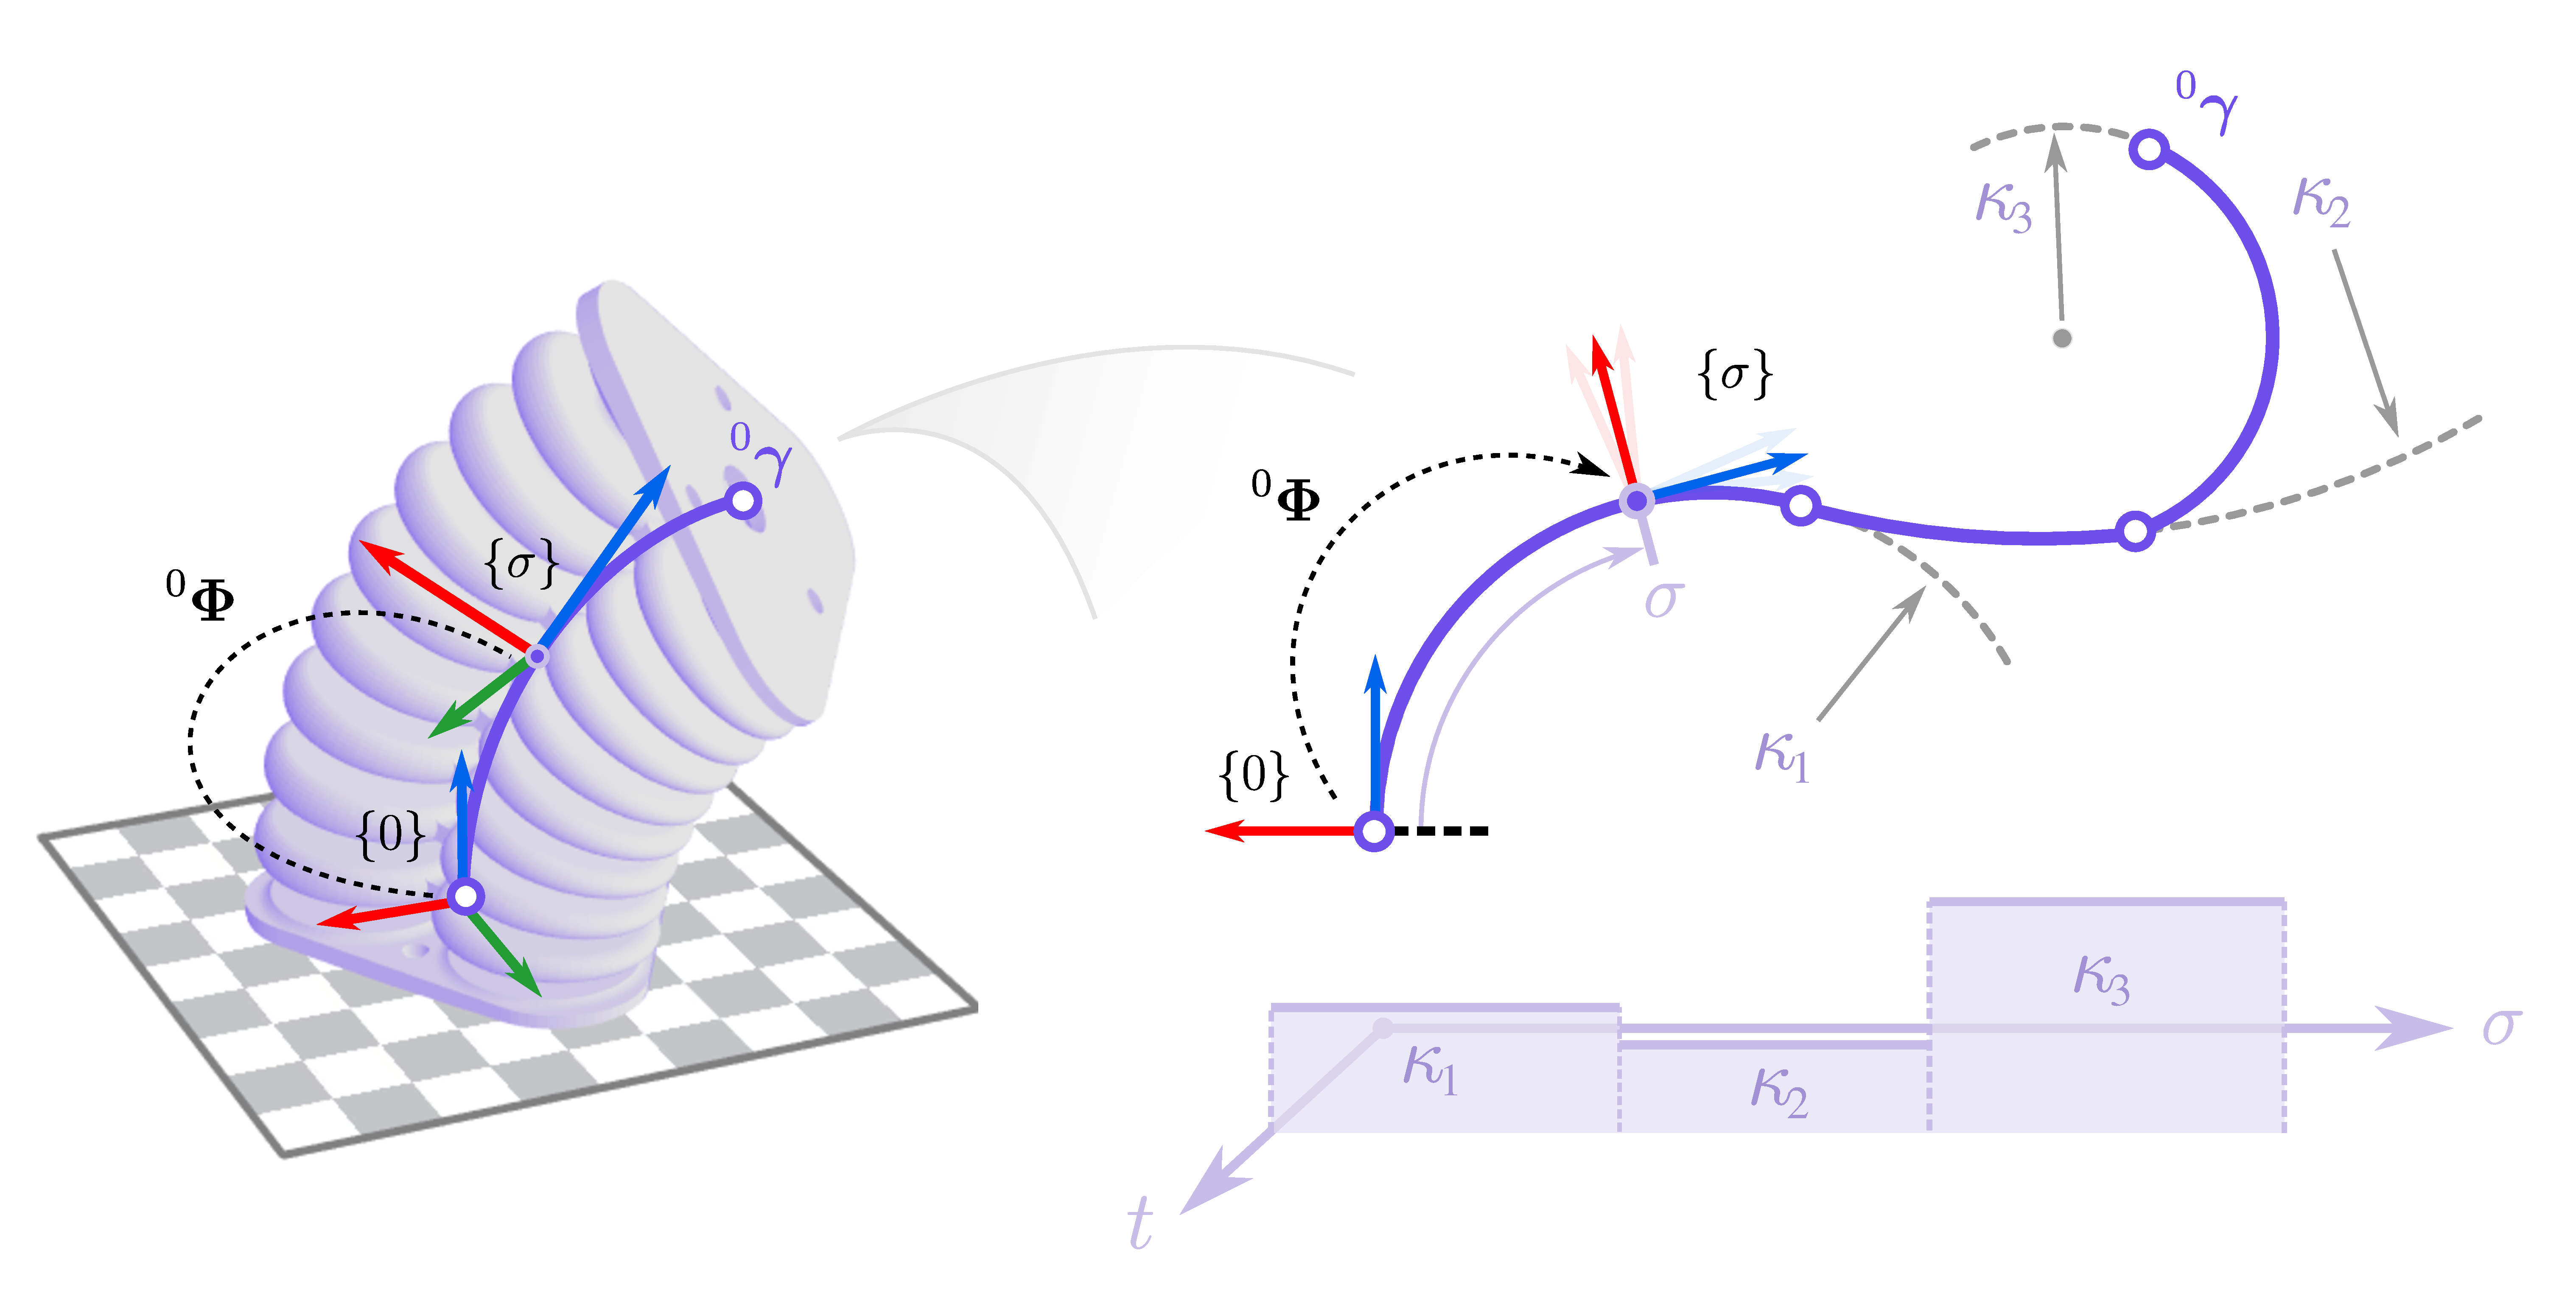
\includegraphics[width = 0.99\textwidth]{fig_C2_schematic.pdf}
  \caption{Schematic representation of the Piece-wise Constant Curvature (PCC) description for general soft \editl manipulator systems\editr, given by a parameterized curve $^0 \gammaB: \Xs \times \mathcal{Q} \to \R^3$ and orientation matrix $^0 \PhiB: \Xs \times \mathcal{Q} \to \SO{3}$. The frame $\{\sigma\}$ is an inertial coordinate frame that evolves over the backbone $^0 \gammaB$ such that variations in $\sigma$ give insight into its differential geometry.}
  \label{fig:C2:configuration}
\end{figure}
%
\begin{asm}[Piece-wise Constant Curvature]
\label{asm:C2:pcc}
Despite the inherent flexibility in soft robotics, it is sometimes sufficient to express the kinematics according to the \emph{Piecewise Constant Curvature} (PCC) condition. \editl This properties often originates from the "\textit{proper}" structural design of the soft robot, where parasitic motion is reduced by structural compliance \editr. Mathematically, it implies that the curvature of the continuous body satisfies $\kappa(\sigma_1,\q) = \kappa(\sigma_2,\q)$ for spatial coordinates on a local region on the soft manipulator $\sigma_1,\sigma_2 \subseteq \Xs$. As a result, this condition allows us to describe the full forward kinematics with a significantly reduced set of generalized coordinates, mitigating kinematic complexity in the model. Numerous works employ PCC models \cite{Falkenhahn2015,Katzschmann2019,Tatlicioglu2007,Marchese2016,Godage2016,DellaSantina2020a}, and depending on the elasticity \editl and structural geometry of the soft robot\editr, the PCC condition has been proven to be consistent for various soft robotic systems.
\end{asm}
%
{Following this Constant Curvature (CC) approach, we assign a coordinate frame that twists minimally along the backbone -- formally called the "\textit{Bishop frame}" (see \cite{Bishop1975}) -- parametrized by the following generalized coordinate vector:}
%
\begin{equation}
\vec{q} := \begin{pmatrix}
\,\varepsilon & \kappa_x & \kappa_y\,
\end{pmatrix}^\top \in \mathcal{Q},
\label{eq:C2:coordinate}
\end{equation}
%
\noindent where $\varepsilon_{-} \le \varepsilon \le \varepsilon_{+}$ is the elongation strain, and $\kappa_x,\,\kappa_y\in\mathbb{R}$ are the curvatures or angular strains in $x$-$z$ and $y$-$z$ plane, respectively; and $\mathcal{Q} \subset \R^3$ is an admissible space on which $\q$ evolves.\editl We will also introduce the following geometric variables\editr $\kappa = \inner{\kappa_x}{\kappa_y}$ and the curvature angle $\phi = \atantwo(\kappa_y,\kappa_x)$. It is worth mentioning that the joint description above is somewhat related to Renda. et al. \cite{Renda2018} who proposed a \emph{Piece-wise Constant Strain} (PCS) parametrization with the exception of including the twist along the tangent.

By exploring the differential geometry of the smooth backbone curve similar to Mochiyama et al. \cite{Mochiyama2003}, we can write the position vector $\gammaB(\sigma,\q)$ and the orientation matrix $\PhiB(\sigma,\q)$ for each material point $\sigma$ along the smooth backbone as a differential equation:
%
\begin{align}
\renewcommand*{\arraystretch}{2}{}
\frac{\partial \,\!\mat{\Phi}}{\partial \sigma}(\sigma,\q) & = \, \mat{\Phi}(\sigma,\vec{q}) \,\mat{\Gamma}^{\times} (\sigma,\q), \label{eq:C2:change_phi} \\[0.75em]
%
\frac{\partial \, \gammaB}{\partial \sigma}(\sigma,\q) & = \, \mat{\Phi}(\sigma,\vec{q}) \, \vec{U}(\sigma,\q), \label{eq:C2:change_p}
\end{align}
%
where \editl $\vec{\Gamma}^\times \in \sog{3}$ \editr is a skew-symmetric matrix composed of the entries of the vector $\vec{\Gamma} \in \R^3$, and $\vec{U}\in \R^3$ a vector representing the tangent along the extensible backbone. The skew-symmetric operator $(\,\cdot\,)^\times$ denotes the isomorphism between the Lie algebra $\sog{3}$ and $\R^3$. The vectors $\vec{\Gamma}$ and $\vec{U}$ are vectors that define the differential geometry of the backbone
\cite{Mochiyama2003} which are unique entries that live in the tangent space of the rigid-body transformation group (\ie, $T_{\SE{3}}$). Given the Bishop parametrization shown in \eqref{eq:C2:coordinate} and assuming the Piecewise Constant-Strain (PCC) condition, these geometric entities yield
%
\begin{align}
\vec{\Gamma}^\times(\sigma,t) & \simeq \vec{\Gamma}^\times(\sigma,\q(t)) \!\!\!\quad \xRightarrow[]{\textrm{\;\;PCC\;\;}}\quad \vec{\Gamma}^\times = \begin{pmatrix} 0 & 0 & \kappa_y \\ 0 & 0 & \kappa_x \\ -\kappa_y & -\kappa_x & 0 \end{pmatrix}, \label{eq:C2:Gamma}\\[0.35em]
%
\vec{U}(\sigma,t) & \simeq \vec{U}(\sigma,\q(t)) \!\quad \xRightarrow[]{\textrm{\;\;PCC\;\;}} \quad \;\; \vec{U} = \;\begin{pmatrix} \;0\;\;  &  \;0\;\; & \varepsilon + 1\ \end{pmatrix}^\top. \label{eq:C2:U}
\end{align}
%
%with $\vec{U}^\circ$ the unit-tangent pointing, and $\vec{\Gamma}^\circ$ the intrinsic curvature/torsion of the curve. For simplicity, lets assume $\vec{U}^\circ = (0,0,1)^\top$ and $\vec{\Gamma}^\circ = \vec{0}_3$.
Now, given an initial configuration of backbone's base, \ie, $\mat{\Phi}(0,\vec{q}) = \vec{\Phi}_0$ and $ \gammaB(0,\q) = \vec{0}_3$, we can now solve for the position and orientation for each material coordinate $\sigma$ along the backbone:
%
\begin{align}
\mat{\Phi}(\sigma,\vec{q}) & = \vec{\Phi}_0\exp_{\SO{3}}(\sigma \vec{\Gamma}^\times(\vec{q})), \label{eq:C2:phi_exact} \\[0.35em]
\gammaB(\sigma,\vec{q}) & = \int_0^\sigma\,^0\mat{\Phi}(s, \vec{q})\, \vec{U}(\vec{q}) \; ds,
\label{eq:C2:pos_exact}
\end{align}
%
where $\exp_{\SO{3}}: \sog{3} \to \SO{3}$ is the exponential map. Luckily, there exists a compact expression for the exponential mapping related to the orthogonal group of rotation matrices $\SO{3}$ called the "\emph{Rodriguez formulas}". \editl The rotation angle along the soft body can be computed by $\theta(\sigma,\q) := \int_0^\sigma \kappa(s,\q) \; ds = \kappa(\q) \sigma$. Notice that the rotation angle $\theta$ linearly depends on $\sigma$, which is a property that follows from Assumption \ref{asm:C2:pcc}. Then, given the expression for the angle of rotation, \editr we can compactly rewrite the rotation matrix \eqref{eq:C2:phi_exact} in terms of $\cos(\theta)$ and $\sin(\theta)$ using these formulas as follows \cite{Lynch2017}:
%
\begin{equation}
\PhiB(\theta) = \PhiB_0 \left( \mat{I}_3 + \left[ \frac{\sin(\theta)}{\theta} \right]  \GammaB^{\times} + \left[ \frac{1-\cos(\theta)}{\theta^2} \right]  \GammaB^{\times} \GammaB^{\times} \right).
\label{eq:C2:phi_rodr}
\end{equation}
%
Note that the closed-form solutions \eqref{eq:C2:phi_exact} and \eqref{eq:C2:pos_exact} represent the forward configuration kinematics of the backbone curve. To express the forward velocity kinematic, let
$\etaB(\sigma,\q,\dq) = \left( \vec{\omega}^\top, \vec{v}^\top \right)^\top \in \R^6 \cong \seg{3}$
 be the aggregate of the angular velocity and linear velocity components relative to an inertial frame at $\sigma$, where the space $\seg{3}$ denotes the Lie algebra of $\SE{3}$. The velocity twist is computed by the following integration procedure:
%
\begin{align}
 \etaB(\sigma,\q,\dq)& = \Ad_{\mat{g}(\sigma,\cdot)}\inv \int_0^\sigma \Ad_{\mat{g}(s,\cdot)}\, \JB^\star\! \dq\;ds, \notag \\ & 
 \,=:\, \JB(\q,\sigma) \dq, \label{eq:C2:vel_cont}
\end{align}
%
where $\Ad_g: \SE{3} \to \mathbb{R}^{6\times 6}$ denotes the adjoint transformation matrix regarding the rigid body transformation $\gB \in \SE{3}$ that maps local velocities (i.e., twist) to a frame located at $\sigma$, and $\JB^\star:\Q \to T_{\q}\Q$ the joint-axis matrix that relates the DOFs to the generalized coordinate description. Let it be clear that the joint-axis matrix is naturally constant for a soft segment modeled with the Constant-Strain (CS) assumption. We will later relax this assumption in Chapter 4. Nevertheless here, the joint-axis matrix for an extensible and bendable CS segment parametrized by the Bishop parameters is given by
%
\begin{align}
\renewcommand*{\arraystretch}{1}{}
\JB^\star := \begin{pmatrix}\dfrac{\p \GammaB}{\p \q}^\top & \dfrac{\p \UB}{\p \q}^\top \end{pmatrix}^\top  = \begin{pmatrix}
\,0 & 0 & 0 & 0 & 0 & 1 \, \\
\,0 & 1 & 0 & 0 & 0 & 0 \,  \\
\,-1 & 0 & 0 & 0 & 0 & 0 \,  \\
\end{pmatrix}^\top. \label{eq:C2:joint-axis-matrix}
\end{align}
%
Although we based the forward kinematics on Mochiyama et al. (2003, \cite{Mochiyama2003}), the derived expression for the velocity twist in \eqref{eq:C2:vel_cont} is analogous to the work of Renda et al. (2018, 2020; \cite{Renda2018,Renda2020}), and Boyer et al. (2010, 2021; \cite{Boyer2010,Boyer2021}). Please also note that
\eqref{eq:C2:vel_cont} gives rise to the geometric manipulator Jacobian $\JB(\sigma,\q)$ that defines the mapping from joint velocities to the velocity twist for a point $\sigma$ on the elastic body.

Given the explicit expression for the velocity twist in \eqref{eq:C2:vel_cont}, we can derive the acceleration twist \cite{Boyer2021,Mochiyama2003,Renda2018} which is obtained through time differentiation of \eqref{eq:C2:vel_cont}:
%
\begin{align}
\dot{\etaB}(\sigma,\q,\dq,\ddq) & = \JB \ddot{\q} + \Ad_{\gB(\cdot,\sigma)} \inv \int_0^\sigma \Ad_{\gB(s,\cdot)}
\ad_{\etaB(s,\cdot,\cdot)} \, \JB^\star\! \dq \;ds \notag \\
& :=  \JB(\sigma,\q)\ddot{\q} + \dmat{J}(\sigma,\q,\dot{\q}) \dot{\q},
\label{eq:C2:acceleration}
\end{align}
%
where $\ad_{\etaB}: \R^{6} \to \R^{6\times 6}$ denotes the adjoint transformation regarding the velocity twist $\vec{\etaB}^\wedge \in \seg{3}$. The reader is referred to Appendix \ref{app:C2:adjoint} for more detailed expressions on the adjoint transformations.
%
\begin{rmk}[Numerical instability near zero-curvature] For many of the PCC modeling frameworks \cite{Falkenhahn2015}, there are mentions of a\editl singularity point or discontinuity of the kinematic formulations at zero-curvature $\kappa = 0$. It is often reported that trajectories that pass through the origin lead to unbounded linear velocities $\vec{v} := \floor{\etaB}_3$, which may result in critical problems in practice. Although it is believed the problem is simply a by-product of the PCC hypothesis, this is however a common misconception, and it stems from a numerical origin.\editr To illustrate this, consider the inextensible planar case: $\varepsilon = \kappa_y = 0$ and $\kappa = \kappa_x$. \editl For simplicity, we assume $L = 1$.\editr Hence, by solving the forward kinematics for the position vector $\gammaB(\sigma,\kappa)$, and approaching zero-curvature from the positive domain $\kappa^{+} \to 0$, we see that
%
\begin{align}
\lim_{\kappa \to \,0^{+}}\gammaB(\sigma,\kappa) & = \begin{pmatrix} \dfrac{1-\cos(\sigma \kappa)}{\kappa}\,, & 0\,, & \dfrac{\sin(\sigma \kappa)}{\kappa} \end{pmatrix}^\top = \begin{pmatrix} 0 & 0 & \sigma \end{pmatrix}^\top,
\end{align}
%
so its limit clearly exists. Since the position vector $\gammaB$ is continuously differentiable when approaching the origin from both sides $\kappa \to 0^+$ and $\kappa \to 0^{-}$, it follows that $\dot{\gammaB}$ must be bounded for all $\kappa \in \Q$. We can simply check this by investigating the behavior of the linear-velocity components of the geometric Jacobian near zero-curvature, which yield
%
\begin{align}
\lim_{\kappa \to \,0^+} \floor{\JB}_3(\sigma,\kappa) & = \begin{pmatrix} \tfrac{\sigma \kappa \sin(\sigma \kappa) + 1 - \cos(\sigma \kappa)}{\kappa^2}\,, & 0\,, & \tfrac{\sigma \kappa \cos(\sigma \kappa) - \sin(\sigma \kappa) }{\kappa^2} \end{pmatrix}^\top \notag \\[0.35em] & = \begin{pmatrix} \sigma^2 & 0 & 0 \end{pmatrix}^\top.
\end{align}
%
\editl Again, its limit exists. Since both limits exist, we define $\vec{\gamma}(\sigma,0):= \lim_{\kappa \to \,0} \vec{\gamma}(\sigma,\kappa)$ and $\vec{J}(\sigma,0):= \lim_{\kappa \to \,0} \vec{J}(\sigma,\kappa)$. Consequently, the magnitude of the linear velocity of the end-effector reads simply $\lVert \dot{\gammaB}(L,\dot{\kappa}) \rVert = L^2\dot{\kappa} = L \omega_1$ with $\omega_1$ the angular velocity at the tip. Moreover, it is bounded for all $\kappa \in \mathcal{Q}$. This naturally poses an ambiguity on the origin of the kinematic singularity so often reported literature.\editr The problem is believed to be of numerical origin when considering the zero-division. To make matters worse, deriving analytical expressions for accelerations will contain similar expressions that are hard to stabilize numerically. To resolve this issue, we opt for a numerical approximation of the forward kinematics -- namely, we employ an explicit forward integration scheme (\ie, trapezoidal integration) to solve \eqref{eq:C2:change_phi} and \eqref{eq:C2:change_p}.
\end{rmk}

\begin{figure}[!h]
  % This file was created by matlab2tikz.
%
%The latest updates can be retrieved from
%  http://www.mathworks.com/matlabcentral/fileexchange/22022-matlab2tikz-matlab2tikz
%where you can also make suggestions and rate matlab2tikz.
%
\definecolor{mycolor1}{rgb}{0.06275,0.35686,0.84706}%
\definecolor{mycolor2}{rgb}{0.86667,0.21176,0.10980}%
\definecolor{mycolor3}{rgb}{0.18039,0.52157,0.25098}%
%
\begin{tikzpicture}

\begin{axis}[%
width=0.259\textwidth,
height=0.215\textwidth,
at={(0\textwidth,0\textwidth)},
scale only axis,
xmin=0,
xmax=5.01,
xlabel style={font=\color{white!15!black}},
xlabel={time (s)},
ymin=-2,
ymax=2,
ylabel style={font=\color{white!15!black}},
ylabel={$\q_d$},
axis background/.style={fill=white},
xmajorgrids,
ymajorgrids,
ylabel style={yshift=-9.5pt}
]
\addplot [color=mycolor1, line width=1.5pt, forget plot]
  table[row sep=crcr]{%
0	0\\
0.0590118023604722	0.0122599350151695\\
0.122024404880976	0.051245683586683\\
0.197039407881577	0.127356433673519\\
0.306061212242448	0.274610958461174\\
0.464092818563713	0.485281744378211\\
0.539107821564313	0.550009396707688\\
0.599119823964793	0.574155119595387\\
0.654130826165233	0.570918154822998\\
0.708141628325666	0.542425923995588\\
0.766153230646129	0.483585222567674\\
0.833166633326665	0.381001848782168\\
0.914182836567313	0.214127314579629\\
1.02820564112823	-0.075581754600881\\
1.25925185037007	-0.672851821290417\\
1.34526905381076	-0.833669846120815\\
1.41328265653131	-0.919160442883364\\
1.47129425885177	-0.95862945224353\\
1.52230446089218	-0.966293478371877\\
1.57331466293259	-0.948199994340202\\
1.62732546509302	-0.90137626204806\\
1.68933786757351	-0.814258548692571\\
1.76335267053411	-0.668276174824877\\
1.85537107421484	-0.435076623934572\\
1.99539907981596	-0.0143847160291388\\
2.19043808761752	0.562122882172909\\
2.28645729145829	0.78232701823107\\
2.36147229445889	0.906026029952742\\
2.4244848969794	0.971401468926922\\
2.47949589917984	0.997472999626086\\
2.53050610122024	0.995067322990411\\
2.58251650330066	0.966335526484759\\
2.63952790558112	0.905286120543856\\
2.70554110822164	0.798558894400302\\
2.78455691138228	0.62627694206536\\
2.8875775155031	0.345873241993202\\
3.26665333066613	-0.743113935603639\\
3.34566913382677	-0.884745361525436\\
3.41068213642729	-0.960888000773404\\
3.46669333866773	-0.994529710207253\\
3.51770354070814	-0.998453103672079\\
3.56871374274855	-0.976789847418135\\
3.624724944989	-0.924209595097784\\
3.68873774754951	-0.829302846512608\\
3.76375275055011	-0.675905403764888\\
3.85977195439088	-0.426427403766472\\
4.0128025605121	0.0402095863869585\\
4.1878375675135	0.556451691884553\\
4.28385677135427	0.778179781889043\\
4.35987197439488	0.904655728387877\\
4.42288457691538	0.970797027717512\\
4.47789557911582	0.997589797446857\\
4.52790558111622	0.996159624088327\\
4.57991598319664	0.968648768140962\\
4.6369273854771	0.908894839975858\\
4.70294058811762	0.803552513256307\\
4.78195639127826	0.632676263537522\\
4.88397679535907	0.356479989904654\\
5	8.88178419700125e-16\\
};
\addplot [color=mycolor2, line width=1.5pt, forget plot]
  table[row sep=crcr]{%
0	0\\
0.138027605521104	0.140440300108925\\
0.211042208441689	0.184935584810103\\
0.272054410882176	0.196656209080302\\
0.329065813162632	0.183310753811706\\
0.388077615523104	0.143577314476932\\
0.454090818163633	0.0688810755447316\\
0.533106621324265	-0.0570083146317186\\
0.645129025805161	-0.281096403013078\\
0.835167033406681	-0.662476511437434\\
0.916183236647329	-0.777169753245791\\
0.980196039207842	-0.832701926306017\\
1.03520704140828	-0.851571468783066\\
1.08621724344869	-0.843577250292476\\
1.13922784556911	-0.808789721087341\\
1.19823964792959	-0.739024227249642\\
1.26625325065013	-0.620955121877476\\
1.3502700540108	-0.427767812642783\\
1.46629325865173	-0.101666846450176\\
1.72234446889378	0.633525295214997\\
1.81136227245449	0.820837424693816\\
1.88337667533507	0.92640916650209\\
1.94338867773555	0.978331555991308\\
1.99639927985597	0.99518363496166\\
2.04740948189638	0.985184790347176\\
2.1004200840168	0.947820917223337\\
2.15943188637728	0.875183689696618\\
2.22844568913783	0.752107632272527\\
2.31346269253851	0.552461842844861\\
2.42848569713943	0.222651201302659\\
2.71854370874175	-0.633815634394776\\
2.80756151230246	-0.822691363947944\\
2.87857571514303	-0.928076540294048\\
2.93858771754351	-0.981414393680224\\
2.99159831966393	-0.999628398951698\\
3.04260852170434	-0.991037597553407\\
3.09561912382476	-0.955207840530338\\
3.15463092618524	-0.884300387785018\\
3.22364472894579	-0.7631603021345\\
3.30766153230646	-0.568142665295742\\
3.42068413682737	-0.246607234578534\\
3.72574514902981	0.65122625379941\\
3.8127625525105	0.831927524141501\\
3.88377675535107	0.93407870842546\\
3.94278855771154	0.983891068491499\\
3.99579915983197	0.999912900564358\\
4.04680936187237	0.989206735619766\\
4.0998199639928	0.951231137729379\\
4.15983196639328	0.876560868859253\\
4.22984596919384	0.750430990306204\\
4.31586317263453	0.546754312000056\\
4.43288657731546	0.209284340535875\\
4.71394278855771	-0.622647147364128\\
4.80396079215843	-0.816268101959198\\
4.87597519503901	-0.925047608943518\\
4.9369873974795	-0.980469837601955\\
4.98999799959992	-0.999506362945193\\
5	-0.999999999998463\\
};
\addplot [color=mycolor3, line width=1.5pt, forget plot]
  table[row sep=crcr]{%
0	-0\\
0.0590118023604722	-0.0323127302272486\\
0.108021604320864	-0.0331290824818566\\
0.157031406281257	-0.0079769875375062\\
0.212042408481697	0.0500216589361884\\
0.283056611322264	0.162185680095956\\
0.485097019403881	0.506055784611869\\
0.536107221444289	0.543684543712172\\
0.578115623124625	0.547118496091529\\
0.619123824764953	0.523782154432988\\
0.664132826565313	0.466781106891244\\
0.718143628725745	0.35651568991531\\
0.785157031406281	0.165020918099894\\
0.890178035607121	-0.209610885997843\\
1.02020404080816	-0.656165846278042\\
1.08621724344869	-0.813331876653166\\
1.13622724544909	-0.8827564770361\\
1.17623524704941	-0.902858557904033\\
1.21324264852971	-0.891876333186355\\
1.25225045009002	-0.849343403567872\\
1.29825965193039	-0.75980970794915\\
1.35527105421084	-0.595513228979666\\
1.43128625725145	-0.304509569554719\\
1.70234046809362	0.802351589692006\\
1.75935187037407	0.927771606903312\\
1.80436087217443	0.980075766519771\\
1.84136827365473	0.990077945444886\\
1.87737547509502	0.970779584879269\\
1.91838367673535	0.914613712496442\\
1.96739347869574	0.80264348414426\\
2.02940588117624	0.600183129717624\\
2.11542308461692	0.238476117081353\\
2.33046609321864	-0.696803833599685\\
2.39647929585917	-0.882732768124136\\
2.44748949789958	-0.969018921052845\\
2.4874974994999	-0.997830617495056\\
2.52250450090018	-0.994023401063271\\
2.55951190238048	-0.960649427962859\\
2.60252050410082	-0.885345365627133\\
2.65653130626125	-0.73993292743766\\
2.72654530906181	-0.482199139020603\\
2.83856771354271	0.0246624641119846\\
2.97559511902381	0.621277881997434\\
3.04660932186437	0.844169225727331\\
3.1006201240248	0.951944439490648\\
3.14362872574515	0.994104036503082\\
3.17963592718544	0.998126097022847\\
3.21564312862573	0.973479302424193\\
3.25665133026605	0.911429266327099\\
3.30666133226645	0.79016811146077\\
3.37067413482697	0.572402197653537\\
3.4626925385077	0.174902851173357\\
3.65173034606921	-0.655626629756043\\
3.72074414882977	-0.862521673164816\\
3.77275455091018	-0.959529089678471\\
3.81476295259052	-0.996173299612285\\
3.85077015403081	-0.996625968608955\\
3.8877775555111	-0.96726798143933\\
3.93078615723145	-0.896391559355475\\
3.98279655931186	-0.76204628869428\\
4.0498099619924	-0.523261917173079\\
4.15183036607321	-0.0698574757930102\\
4.30986197239448	0.62473490045429\\
4.38087617523505	0.846533085581687\\
4.43488697739548	0.953293435683277\\
4.47789557911582	0.994579768326681\\
4.51390278055611	0.997854639446826\\
4.55091018203641	0.971359701253584\\
4.59291858371674	0.905657492920928\\
4.64392878575715	0.778672904138067\\
4.70994198839768	0.549251284827934\\
4.80596119223845	0.128630790373577\\
4.97999599919984	-0.637409462896398\\
5	-0.707106781185458\\
};
\end{axis}

\begin{axis}[%
width=0.259\textwidth,
height=0.215\textwidth,
at={(0.341\textwidth,0\textwidth)},
scale only axis,
xmin=0,
xmax=5.01,
xlabel style={font=\color{white!15!black}},
xlabel={time (s)},
ymin=-6,
ymax=6,
ylabel style={font=\color{white!15!black}},
ylabel={$\dq_d$},
axis background/.style={fill=white},
xmajorgrids,
ymajorgrids,
ylabel style={yshift=-9.5pt}
]
\addplot [color=mycolor1, line width=1.5pt, forget plot]
  table[row sep=crcr]{%
0	0.00354490068904045\\
0.137027405481096	0.903588308385592\\
0.206041208241649	1.22856452598255\\
0.257051410282056	1.38060740669893\\
0.296059211842368	1.43857878332504\\
0.326065213042608	1.44671619310838\\
0.356071214242848	1.42249130990263\\
0.39007801560312	1.3560092907744\\
0.432086417283457	1.21821465698646\\
0.485097019403881	0.962586034545687\\
0.553110622124425	0.520529889641796\\
0.651130226045209	-0.270803972466815\\
0.857171434286857	-1.96111846971092\\
0.93118623724745	-2.39268873749415\\
0.988197639527906	-2.61578401240715\\
1.03220644128826	-2.71435218975166\\
1.06621324264853	-2.74427973959115\\
1.09621924384877	-2.73665215168262\\
1.12822564512903	-2.69342117279692\\
1.16623324664933	-2.59588760182128\\
1.21324264852971	-2.40873834185884\\
1.27225445089018	-2.07805095116542\\
1.34626925385077	-1.53498416704634\\
1.44928985797159	-0.609800554006279\\
1.7373474694939	2.06478538831989\\
1.81936387277455	2.60307834026396\\
1.88337667533507	2.90062171255517\\
1.93538707741548	3.05371910764113\\
1.97639527905581	3.11545185690039\\
2.00840168033607	3.12679834073453\\
2.03940788157632	3.10692697008051\\
2.0744148829766	3.04832587668127\\
2.11742348469694	2.92503238525876\\
2.16943388677736	2.70379607461824\\
2.23344668933787	2.33206311088885\\
2.31346269253851	1.73595350618949\\
2.42348469693939	0.745755428207096\\
2.72054410882176	-2.00968788046552\\
2.80556111222244	-2.57586752681016\\
2.87157431486297	-2.89102311132145\\
2.9245849169834	-3.05482622701098\\
2.96659331866373	-3.12471640436199\\
2.999599919984	-3.14152189462515\\
3.03060612122425	-3.12655715277568\\
3.06461292258452	-3.0760658872595\\
3.10662132426485	-2.96535682645882\\
3.15663132626525	-2.76652815312306\\
3.21864372874575	-2.42602567294836\\
3.29565913182637	-1.8771253886638\\
3.39767953590718	-0.987885846273739\\
3.75075015003001	2.23014715782088\\
3.82876575315063	2.70040323156362\\
3.89077815563113	2.96011198400992\\
3.93978795759152	3.08647630578385\\
3.97879575915183	3.13494797811861\\
4.01080216043209	3.1396111777881\\
4.04280856171234	3.11255800697227\\
4.07981596319264	3.04211546348687\\
4.124824964993	2.90122307727425\\
4.17983596719344	2.65075511896351\\
4.24684936987398	2.23986170977253\\
4.33186637327465	1.57905334730502\\
4.45289057811562	0.458374253608507\\
4.69693938787758	-1.82607588925665\\
4.7869573914783	-2.46688451700194\\
4.85697139427886	-2.83188138573282\\
4.9129825965193	-3.02625903108539\\
4.95799159831966	-3.11491811053946\\
4.99299859971994	-3.14093609486879\\
5	-3.14158748587636\\
};
\addplot [color=mycolor2, line width=1.5pt, forget plot]
  table[row sep=crcr]{%
0	1.12837322264768\\
0.0290058011602321	1.11287690718957\\
0.0620124024804962	1.05918703548886\\
0.103020604120824	0.940995733860333\\
0.154030806161233	0.720852429683366\\
0.221044208841769	0.329040615346998\\
0.324064812962592	-0.415015201309904\\
0.479095819163833	-1.51762477223098\\
0.550110022004401	-1.88091677154614\\
0.603120624124825	-2.05657754379251\\
0.643128625725145	-2.12690523971632\\
0.674134826965394	-2.14233493262017\\
0.703140628125626	-2.12518565975495\\
0.736147229445889	-2.06847786435016\\
0.776155231046209	-1.94764697173144\\
0.826165233046609	-1.72032118445276\\
0.888177635527105	-1.33287793109094\\
0.970194038807762	-0.677703297361942\\
1.1122224444889	0.656669942201704\\
1.25425085017003	1.92027334813605\\
1.33826765353071	2.4957239295581\\
1.40328065613123	2.8110209600663\\
1.45429085817163	2.96740997845937\\
1.49429885977195	3.03077028972536\\
1.52630526105221	3.04316268415615\\
1.55631126225245	3.0238292307504\\
1.59131826365273	2.96385353194767\\
1.63332666533307	2.84010088177006\\
1.68533706741348	2.61261209274866\\
1.74934986997399	2.23016785497343\\
1.83036607321464	1.61058449856721\\
1.94538907781556	0.55355301879334\\
2.20544108821764	-1.88333064164048\\
2.29345869173835	-2.49961881538618\\
2.3624724944989	-2.85081712197516\\
2.41748349669934	-3.03514561937135\\
2.46149229845969	-3.11735537496245\\
2.49549909981996	-3.14000923889623\\
2.52650530106021	-3.12935139813733\\
2.56051210242048	-3.08346030159967\\
2.6005201040208	-2.9844099202232\\
2.6505301060212	-2.79450937790965\\
2.71154230846169	-2.47007506810393\\
2.78655731146229	-1.94858631705674\\
2.88457691538308	-1.10996961666554\\
3.10262052410482	0.99996718143458\\
3.22164432886577	2.01874975626282\\
3.30566113222645	2.57684537272085\\
3.37167433486697	2.89165495774407\\
3.4246849369874	3.05520852382526\\
3.46669333866773	3.12491681950401\\
3.499699939988	3.14158841415858\\
3.53070614122825	3.12650471358071\\
3.56471294258852	3.07589032073885\\
3.60672134426885	2.96503961364553\\
3.65673134626925	2.76605754535741\\
3.71874374874975	2.42538893386612\\
3.79575915183037	1.87632266950521\\
3.89777955591118	0.986940126259217\\
4.25085017003401	-2.23084317749245\\
4.32886577315463	-2.70090796640865\\
4.39087817563513	-2.96044270093426\\
4.43988797759552	-3.08666036495903\\
4.47889577915583	-3.13501205318945\\
4.51090218043609	-3.13957601885231\\
4.54290858171634	-3.11242397791472\\
4.57991598319664	-3.04186887567698\\
4.624924984997	-2.9008442325007\\
4.67993598719744	-2.65022515672919\\
4.74694938987798	-2.23916940295443\\
4.83196639327866	-1.57819986384533\\
4.95299059811962	-0.457397634949563\\
5	0.00493479812624376\\
};
\addplot [color=mycolor3, line width=1.5pt, forget plot]
  table[row sep=crcr]{%
0	-0.794115508462454\\
0.0580116023204642	-0.277364611734568\\
0.26505301060212	1.70491593082617\\
0.306061212242448	1.87842338112035\\
0.334066813362672	1.92300384411942\\
0.356071214242848	1.91292691038186\\
0.38007601520304	1.85542433262415\\
0.411082216443289	1.70919219099674\\
0.451090218043609	1.40465740373763\\
0.504100820164033	0.820935563376146\\
0.578115623124625	-0.248600075058891\\
0.762152430486097	-2.99671953899652\\
0.816163232646529	-3.4867860854134\\
0.855171034206841	-3.68308225183768\\
0.882176435287057	-3.73307210749446\\
0.902180436087217	-3.72294329754286\\
0.924184836967394	-3.66485742913014\\
0.954190838167634	-3.50676773602809\\
0.993198639727946	-3.16939676216821\\
1.04320864172835	-2.53683562435458\\
1.11022204440888	-1.40251215395337\\
1.23224644928986	1.09146932720294\\
1.34026805361072	3.11962860739989\\
1.40428085617123	3.97847580467464\\
1.45229045809162	4.38259317834563\\
1.4872974594919	4.53109137402165\\
1.51030206041208	4.55856842712607\\
1.53030606121224	4.53675451436047\\
1.55431086217243	4.45469330662973\\
1.58631726345269	4.25233666981845\\
1.62832566513303	3.83346415954477\\
1.68233646729346	3.06612040251519\\
1.75535107021404	1.70902193090805\\
2.03440688137628	-3.80704018778977\\
2.08841768353671	-4.38067909824091\\
2.12942588517704	-4.62780828971085\\
2.15843168633727	-4.6982027777484\\
2.17843568713743	-4.69538596539201\\
2.1994398879776	-4.64729630338051\\
2.22744548909782	-4.5121578146679\\
2.26445289057812	-4.21315733318806\\
2.3124624924985	-3.63571053810641\\
2.374474894979	-2.61980512471882\\
2.46549309861972	-0.754128407877475\\
2.6495299059812	3.05964290826855\\
2.71654330866173	4.02147655398821\\
2.76655331066213	4.48381747958504\\
2.80356071214243	4.66721925102645\\
2.82956591318264	4.71152470359658\\
2.84856971394279	4.69919553002523\\
2.87157431486297	4.63390058682298\\
2.90158031606321	4.46715113358115\\
2.94058811762353	4.11776373765277\\
2.99059811962393	3.4689862272862\\
3.05761152230446	2.30691776642933\\
3.16363272654531	0.0563190270418401\\
3.30666133226645	-2.89690138385146\\
3.37667533506701	-3.9448221542987\\
3.42868573714743	-4.45241981565303\\
3.46769353870774	-4.65954561876156\\
3.49469893978796	-4.71117486462973\\
3.51470294058812	-4.70029361858979\\
3.53670734146829	-4.64013279511158\\
3.56671334266853	-4.47797683817697\\
3.60572114422885	-4.13425107699655\\
3.65573114622925	-3.49192821143007\\
3.72174434886977	-2.35576737664234\\
3.82576515303061	-0.156931641015601\\
3.97379475895179	2.90509369151093\\
4.04380876175235	3.950496362776\\
4.09581916383277	4.45581244484655\\
4.13482696539308	4.66108744519533\\
4.16183236647329	4.71140168604915\\
4.18183636727345	4.69954306835578\\
4.20484096819364	4.63434132500523\\
4.23484696939388	4.46772453283112\\
4.27385477095419	4.11851887812703\\
4.32386477295459	3.46996990086312\\
4.39087817563513	2.30815865696121\\
4.49689937987598	0.0577494594312666\\
4.63992798559712	-2.89575760597693\\
4.70994198839768	-3.94402589682519\\
4.7619523904781	-4.45194298479568\\
4.80096019203841	-4.65932964437099\\
4.82796559311862	-4.71114488543943\\
4.84796959391878	-4.70040215831249\\
4.86997399479896	-4.64039276611033\\
4.8999799959992	-4.47843880303433\\
4.93898779755951	-4.13496168317129\\
4.98899779955991	-3.49292197179463\\
5	-3.32429866327344\\
};
\end{axis}

\begin{axis}[%
width=0.259\textwidth,
height=0.215\textwidth,
at={(0.682\textwidth,0\textwidth)},
scale only axis,
xmin=0,
xmax=5.01,
xlabel style={font=\color{white!15!black}},
xlabel={time (s)},
ymin=-30,
ymax=30,
ylabel style={font=\color{white!15!black}},
ylabel={$\ddq_d$},
axis background/.style={fill=white},
xmajorgrids,
ymajorgrids,
ylabel style={yshift=-9.5pt}
]
\addplot [color=mycolor1, line width=1.5pt, forget plot]
  table[row sep=crcr]{%
0	7.08971722508816\\
0.0170034006801352	7.06254176227866\\
0.0380076015203041	6.96211357748433\\
0.0670134026805353	6.70383363218785\\
0.105021004200839	6.16331809076554\\
0.15503100620124	5.13123086154366\\
0.221044208841768	3.30313004756611\\
0.322064412882577	-0.140715150531712\\
0.483096619323865	-5.57492932673487\\
0.555111022204441	-7.34242512612227\\
0.609121824364873	-8.2298345369658\\
0.650130026005201	-8.61942170460317\\
0.679135827165434	-8.74010611151554\\
0.696139227845569	-8.75056964311227\\
0.714142828565713	-8.71323899853671\\
0.738147629525905	-8.58686459570546\\
0.770154030806161	-8.28547401565682\\
0.812162432486497	-7.67074463808859\\
0.866173234646929	-6.54917377090891\\
0.937187437487498	-4.60734590265721\\
1.04320864172835	-1.07483524322571\\
1.24624924984997	5.72961331213317\\
1.32926585317063	7.81639650559995\\
1.39427885577116	8.9859331390274\\
1.44528905781156	9.58253887084481\\
1.48529705941188	9.8442837551671\\
1.51330266053211	9.91865276034343\\
1.53230646129226	9.91831589369774\\
1.55331066213243	9.87066630009359\\
1.58031606321264	9.73764473499728\\
1.61632326465293	9.43822354992907\\
1.6623324664933	8.86253703324957\\
1.72034406881376	7.8537245560284\\
1.79335867173435	6.19915830635254\\
1.89137827565513	3.47504190478798\\
2.25345069013803	-7.05759085861679\\
2.32946589317864	-8.49825043913732\\
2.39047809561912	-9.30375995789046\\
2.4374874974995	-9.69098733938356\\
2.47349469893979	-9.84429919326235\\
2.49849969993999	-9.87645177319418\\
2.51850370074015	-9.85815891485498\\
2.54250850170034	-9.78470810142351\\
2.5745149029806	-9.6001934501988\\
2.61552310462092	-9.22223443122761\\
2.66653330666133	-8.53959500779489\\
2.72954590918184	-7.39663922633138\\
2.80856171234247	-5.56189473532864\\
2.91558311662332	-2.55857583281172\\
3.22764552910582	6.49527125262672\\
3.30966193238648	8.17448519252473\\
3.374674934987	9.12633838257015\\
3.42568513702741	9.60899637547641\\
3.46469293858772	9.81236106656347\\
3.49269853970794	9.86769341093652\\
3.5127025405081	9.86048208595491\\
3.53570714142829	9.80407057871169\\
3.56471294258852	9.66005045055507\\
3.60272054410882	9.35027485493567\\
3.65073014602921	8.7694054033971\\
3.70974194838968	7.78440013127213\\
3.78275655131026	6.20094073200406\\
3.87877575515103	3.63970724426288\\
4.05881176235247	-1.84364405983484\\
4.19783956791358	-5.77205567675598\\
4.2868573714743	-7.75761622429094\\
4.35587117423485	-8.88854079805768\\
4.41088217643529	-9.49382693860024\\
4.45389077815563	-9.77065608576133\\
4.48489697939588	-9.85991079216486\\
4.50590118023605	-9.86727677343424\\
4.52690538107622	-9.83169388013572\\
4.55391078215643	-9.72310658142739\\
4.58891778355671	-9.47842189369386\\
4.63392678535707	-8.99611634308517\\
4.68893778755751	-8.16403545489397\\
4.75695139027806	-6.80236720584926\\
4.84396879375875	-4.61913345423115\\
4.97299459891978	-0.805433305647973\\
5	0.0310062018553658\\
};
\addplot [color=mycolor2, line width=1.5pt, forget plot]
  table[row sep=crcr]{%
0	-0.0356665298542058\\
0.14002800560112	-4.67099677947669\\
0.210042008401681	-6.35787080027761\\
0.262052410482097	-7.18121414389206\\
0.301060212042408	-7.52419844540775\\
0.328065613122625	-7.61679085886646\\
0.34506901380276	-7.61344158614619\\
0.364072814562913	-7.55338671970529\\
0.390078015603121	-7.3759254387018\\
0.425085017003401	-6.96795293714247\\
0.47009401880376	-6.17536023821841\\
0.528105621124224	-4.76203193936642\\
0.608121624324864	-2.2616035058598\\
0.90118023604721	7.41655342073599\\
0.965193038607721	8.68477119764233\\
1.01520304060812	9.31550428917571\\
1.05321064212843	9.57115136568376\\
1.07921584316863	9.63325353187106\\
1.09821964392879	9.62095442347266\\
1.12022404480896	9.54664003094408\\
1.14922984596919	9.35230091148043\\
1.1872374474895	8.93817915492701\\
1.23624724944989	8.15570308454472\\
1.29825965193039	6.81305056038362\\
1.38127625525105	4.53205984490834\\
1.51730346069214	0.137104630163254\\
1.6873374674935	-5.19413042832095\\
1.77835567113423	-7.44111083206267\\
1.8493698739748	-8.73764863851267\\
1.90638127625525	-9.44363453025954\\
1.95139027805561	-9.77614657982073\\
1.98439687937588	-9.89060722533797\\
2.00640128025605	-9.90571841918975\\
2.02640528105621	-9.87708129185361\\
2.05241048209642	-9.77998577411654\\
2.08541708341668	-9.56077689839852\\
2.12842568513703	-9.11882330623115\\
2.18143628725745	-8.34382797509914\\
2.24744948989798	-7.05721408722493\\
2.33146629325865	-4.99130619335819\\
2.45249049809962	-1.45521934033521\\
2.69453890778156	5.68634972386572\\
2.78455691138228	7.71289662082619\\
2.85457091418284	8.87123751025509\\
2.90958191638328	9.48327346161904\\
2.95259051810362	9.76549714637454\\
2.98459691938388	9.86011816772603\\
3.00560112022404	9.86808705516484\\
3.02660532106421	9.83309714619462\\
3.05361072214443	9.72525700271287\\
3.08861772354471	9.48151268853614\\
3.13262652530506	9.01304744316267\\
3.1876375275055	8.18694988291568\\
3.25565113022605	6.83174606330716\\
3.34266853370674	4.65484935746607\\
3.47069413882777	0.876546802294875\\
3.6877375475095	-5.51511477797639\\
3.77975595119024	-7.61957450245987\\
3.85077015403081	-8.81865742330401\\
3.90678135627125	-9.45828980758456\\
3.95079015803161	-9.75661509139414\\
3.98279655931186	-9.85681253462545\\
4.00480096019204	-9.86795820689945\\
4.02580516103221	-9.8346227153101\\
4.05281056211242	-9.72890484618461\\
4.0868173634727	-9.4963693895167\\
4.13082616523305	-9.03523157269603\\
4.18483696739348	-8.23480517953001\\
4.25185037007402	-6.91608604630467\\
4.33686737347469	-4.81255275530668\\
4.46089217843569	-1.17876018750085\\
4.69093818763753	5.59713704895159\\
4.78195639127826	7.66275629837665\\
4.85197039407882	8.8353040648137\\
4.90798159631926	9.46885282937515\\
4.95199039807962	9.76215955428295\\
4.98399679935987	9.85863512259488\\
5	9.86954757942193\\
};
\addplot [color=mycolor3, line width=1.5pt, forget plot]
  table[row sep=crcr]{%
0	7.5744225756329\\
0.0520104020804162	9.85795253565652\\
0.0890178035607114	10.7343646901029\\
0.113022604520904	10.9368263420187\\
0.126025205041007	10.9227666810555\\
0.142028405681135	10.7856109086146\\
0.16503300660132	10.3588706857098\\
0.197039407881576	9.32929431048124\\
0.240048009601921	7.21344321073802\\
0.300060012002401	3.12899615273476\\
0.541108221644329	-14.5767064028135\\
0.583116623324663	-15.8947102220086\\
0.611122224444888	-16.2686397032763\\
0.622124424884976	-16.3000792190449\\
0.634126825365072	-16.2590964666309\\
0.651130226045208	-16.0662320020655\\
0.67613522704541	-15.4974275623498\\
0.710142028405681	-14.1945663307275\\
0.75515103020604	-11.6027109979822\\
0.816163232646531	-6.78180501212378\\
0.918183636727345	3.19925678471389\\
1.0372074414883	14.2630289394763\\
1.1002200440088	18.3769434543013\\
1.14622924584917	20.2284519962292\\
1.17923584716943	20.8825917599187\\
1.19923984796959	20.9940018330856\\
1.21024204840968	20.9627983709382\\
1.22624524904981	20.8005305254444\\
1.25025005001	20.300173284471\\
1.28325665133027	19.1232943641539\\
1.32726545309062	16.7321518603769\\
1.38527705541108	12.3448435289664\\
1.46929385877175	4.24762456605077\\
1.66433286657331	-15.006835410114\\
1.72834566913383	-19.2314865141707\\
1.77635527105421	-21.2288700042196\\
1.81136227245449	-21.9820872663368\\
1.83336667333467	-22.1406342791886\\
1.84536907381476	-22.1238119583189\\
1.86137227445489	-21.9881962890689\\
1.88437687537508	-21.5687174401902\\
1.91638327665533	-20.5551161436279\\
1.95839167833567	-18.5063456770163\\
2.01340268053611	-14.7274455786217\\
2.08841768353671	-8.02930998083884\\
2.35847169433887	17.4889091607566\\
2.41448289657932	20.4580950794453\\
2.45649129825965	21.7593237376024\\
2.48549709941988	22.1621020797258\\
2.49949989997999	22.2084088691288\\
2.51150230046009	22.1710021117705\\
2.52850570114023	21.9964824567098\\
2.55351070214043	21.4835583106643\\
2.5875175035007	20.3092524488913\\
2.63252650530106	17.9608482179239\\
2.69053810762152	13.7652243370479\\
2.77155431086217	6.27861523427864\\
3.00360072014403	-16.0384936526148\\
3.06461292258452	-19.7357108331353\\
3.11062212442489	-21.463698030133\\
3.14362872574515	-22.0870363960568\\
3.16463292658532	-22.2064523468513\\
3.17663532706541	-22.1770731289039\\
3.19263852770554	-22.0276153410914\\
3.21664332866573	-21.5691020724051\\
3.249649929986	-20.4902631329995\\
3.29265853170634	-18.3476492789936\\
3.34866973394679	-14.44841849918\\
3.4256851370274	-7.52047923802124\\
3.68573714742949	17.1151521202173\\
3.74374874974995	20.2996418279255\\
3.78675735147029	21.6963760554245\\
3.81676335267053	22.146824126934\\
3.83276655331066	22.2065248116632\\
3.84476895379076	22.1684518725285\\
3.86177235447089	21.9932254539312\\
3.88677735547109	21.479711348027\\
3.92078415683137	20.3053143584819\\
3.96579315863173	17.9577095353878\\
4.02380476095219	13.7639924762123\\
4.10482096419284	6.28037173283591\\
4.3368673734747	-16.0343061430535\\
4.39787957591518	-19.7326927237063\\
4.44388877775555	-21.4618857962146\\
4.47689537907582	-22.0862019015833\\
4.49789957991598	-22.2062702477377\\
4.50990198039608	-22.1772700763623\\
4.52590518103621	-22.0283212123418\\
4.5499099819964	-21.5705710293612\\
4.58291658331666	-20.4927599587457\\
4.62592518503701	-18.3514020697384\\
4.68193638727746	-14.4535738878515\\
4.75895179035807	-7.52695343386733\\
5	15.7762366578273\\
};
\end{axis}
\end{tikzpicture}%
  \vspace{-5mm}
  \caption{The time evolution of the predefined geometric strain parameters of the Piece-wise Constant curvature model $\q_d \to  (\varepsilon, \, \kappa_x,\,\kappa_y)^\top$ and their corresponding time-derivatives $\dq_d$ and $\ddq_d$, given by the (spatially constant) elongation $\varepsilon$ \data{Matlab1}, and the \editl (spatially constant)\editr curvatures $\kappa_x$ \data{Matlab2} and $\kappa_y$ \data{Matlab3}.}
  \label{fig:C2:EX1:strain_ref}
\end{figure}

\begin{example}[Kinematic behavior of PCC segment]
As an illustrative example, we perform a numerical simulation of the forward kinematics for a single PCC segment.\editl We select a differentiable reference trajectory $\q(t) \equiv \q_d(t)$, $\dot{\q}(t) \equiv \dot{\q}_d(t)$ and $\ddot{\q}(t) \equiv \ddot{\q}_d(t)$ that passes the zero-curvature point  given by \editr:
%
\begin{align*}
\q_d(t) &  =  \erf(t) \cdot \begin{pmatrix} \varepsilon_0 \sin(\omega t) & \kappa_0 \cos(\omega t) & \kappa_0 \sin(\tfrac{3}{2}\omega t - \tfrac{\pi}{4}) \end{pmatrix}^\top,
\end{align*}
%
where $\textrm{erf}(t) := \frac{2}{\pi}\int_0^\tau \exp(-\tau^2) \; d\tau$ is referred to as the error function. Note that these are smooth functions such that reference velocity $\dq_d$ and reference acceleration $\ddq_d$ exist and are bounded. The reference signals for the geometric strain of the soft robot are shown in Figure \ref{fig:C2:EX1:strain_ref}. Please note that the reference $\q_d$ has been carefully selected to ensure it passes the line $\kappa_x = \kappa_y = 0$ on the configuration manifold
$\mathcal{Q}$, \ie, the numerical instability point for (near) zero-curvature.

Then, by injecting the reference into the kinematic relations given by \eqref{eq:C2:change_phi}, \eqref{eq:C2:change_p}, \eqref{eq:C2:vel_cont}, and \eqref{eq:C2:acceleration}, we obtain a (close) approximation of forward kinematics as shown in Figure
\ref{fig:C2:EX1:strain_ref_FK}. Furthermore, we provided a 3D-rendering of the soft robot subjected to the reference $\q_d$ in Figure \ref{fig:C2:EX1:strain_ref_3D}. Now, two key observations can be made. First, although a simple harmonic trajectory is used, the resulting trajectory of the end-effector as shown in Figure \ref{fig:C2:EX1:strain_ref_FK} is rather complex. This perhaps stresses the importance of inverse kinematic solver that can be used for task-space control. Second, although we pass the point of numerical instability for $\kappa \to 0$, we see that the velocity solutions are smooth and bounded at these instances. This result shows our approach does not suffer from the near-zero curvature instabilities that are notoriously mentioned in \cite{Falkenhahn2015,DellaSantina2020}. 
\end{example}

\begin{figure}[!h]
   \centering
   \vspace{-2mm}
   % This file was created by matlab2tikz.
%
%The latest updates can be retrieved from
%  http://www.mathworks.com/matlabcentral/fileexchange/22022-matlab2tikz-matlab2tikz
%where you can also make suggestions and rate matlab2tikz.
%
\begin{tikzpicture}

\begin{axis}[%
width=0.216\textwidth,
height=0.199\textwidth,
at={(0\textwidth,0.253\textwidth)},
scale only axis,
axis on top,
xmin=0.5,
xmax=522.5,
tick align=outside,
y dir=reverse,
ymin=0.5,
ymax=458.5,
axis line style={draw=none},
ticks=none,
ylabel style={yshift=-7.5pt}
]
\addplot [forget plot] graphics [xmin=0.5, xmax=522.5, ymin=0.5, ymax=458.5] {fig_plotrobot-1.png};
\end{axis}

\begin{axis}[%
width=0.216\textwidth,
height=0.199\textwidth,
at={(0.245\textwidth,0.253\textwidth)},
scale only axis,
axis on top,
xmin=0.5,
xmax=522.5,
tick align=outside,
y dir=reverse,
ymin=0.5,
ymax=458.5,
axis line style={draw=none},
ticks=none,
ylabel style={yshift=-7.5pt}
]
\addplot [forget plot] graphics [xmin=0.5, xmax=522.5, ymin=0.5, ymax=458.5] {fig_plotrobot-2.png};
\end{axis}

\begin{axis}[%
width=0.216\textwidth,
height=0.199\textwidth,
at={(0.49\textwidth,0.253\textwidth)},
scale only axis,
axis on top,
xmin=0.5,
xmax=522.5,
tick align=outside,
y dir=reverse,
ymin=0.5,
ymax=458.5,
axis line style={draw=none},
ticks=none,
ylabel style={yshift=-7.5pt}
]
\addplot [forget plot] graphics [xmin=0.5, xmax=522.5, ymin=0.5, ymax=458.5] {fig_plotrobot-3.png};
\end{axis}

\begin{axis}[%
width=0.216\textwidth,
height=0.199\textwidth,
at={(0.734\textwidth,0.253\textwidth)},
scale only axis,
axis on top,
xmin=0.5,
xmax=522.5,
tick align=outside,
y dir=reverse,
ymin=0.5,
ymax=458.5,
axis line style={draw=none},
ticks=none,
ylabel style={yshift=-7.5pt}
]
\addplot [forget plot] graphics [xmin=0.5, xmax=522.5, ymin=0.5, ymax=458.5] {fig_plotrobot-4.png};
\end{axis}

\begin{axis}[%
width=0.216\textwidth,
height=0.199\textwidth,
at={(0\textwidth,0\textwidth)},
scale only axis,
axis on top,
xmin=0.5,
xmax=522.5,
tick align=outside,
y dir=reverse,
ymin=0.5,
ymax=458.5,
axis line style={draw=none},
ticks=none,
ylabel style={yshift=-7.5pt}
]
\addplot [forget plot] graphics [xmin=0.5, xmax=522.5, ymin=0.5, ymax=458.5] {fig_plotrobot-5.png};
\end{axis}

\begin{axis}[%
width=0.216\textwidth,
height=0.199\textwidth,
at={(0.245\textwidth,0\textwidth)},
scale only axis,
axis on top,
xmin=0.5,
xmax=522.5,
tick align=outside,
y dir=reverse,
ymin=0.5,
ymax=458.5,
axis line style={draw=none},
ticks=none,
ylabel style={yshift=-7.5pt}
]
\addplot [forget plot] graphics [xmin=0.5, xmax=522.5, ymin=0.5, ymax=458.5] {fig_plotrobot-6.png};
\end{axis}

\begin{axis}[%
width=0.216\textwidth,
height=0.199\textwidth,
at={(0.49\textwidth,0\textwidth)},
scale only axis,
axis on top,
xmin=0.5,
xmax=522.5,
tick align=outside,
y dir=reverse,
ymin=0.5,
ymax=458.5,
axis line style={draw=none},
ticks=none,
ylabel style={yshift=-7.5pt}
]
\addplot [forget plot] graphics [xmin=0.5, xmax=522.5, ymin=0.5, ymax=458.5] {fig_plotrobot-7.png};
\end{axis}

\begin{axis}[%
width=0.216\textwidth,
height=0.199\textwidth,
at={(0.734\textwidth,0\textwidth)},
scale only axis,
axis on top,
xmin=0.5,
xmax=522.5,
tick align=outside,
y dir=reverse,
ymin=0.5,
ymax=458.5,
axis line style={draw=none},
ticks=none,
ylabel style={yshift=-7.5pt}
]
\addplot [forget plot] graphics [xmin=0.5, xmax=522.5, ymin=0.5, ymax=458.5] {fig_plotrobot-8.png};
\end{axis}
\end{tikzpicture}%
   %\vspace{-2mm}
   \caption{Three-dimensional deformation of the three-bellow soft robot manipulator using the PCC model. Based on the prescribed reference $\q_d$ (and its time-derivative $\dq_d$), the forward kinematic relations for each point $\sigma$ along the backbone is computed and the volumetric mesh is deformed accordingly to its closest material-point on $\gammaB(\sigma)$.}
   \vspace{-0.1cm}
   \label{fig:C2:EX1:strain_ref_3D}
 \end{figure}
 %
 \begin{figure}[!t]
  \pgfplotsset{colormap name=barney}
  % This file was created by matlab2tikz.
%
\definecolor{mycolor1}{rgb}{0.89290,0.89290,0.89290}%
\definecolor{mycolor2}{rgb}{0.88840,0.88720,0.89330}%
\definecolor{mycolor3}{rgb}{0.88390,0.88140,0.89360}%
\definecolor{mycolor4}{rgb}{0.87940,0.87570,0.89400}%
\definecolor{mycolor5}{rgb}{0.87490,0.87000,0.89440}%
\definecolor{mycolor6}{rgb}{0.87040,0.86420,0.89470}%
\definecolor{mycolor7}{rgb}{0.86590,0.85850,0.89510}%
\definecolor{mycolor8}{rgb}{0.86140,0.85280,0.89550}%
\definecolor{mycolor9}{rgb}{0.85690,0.84700,0.89590}%
\definecolor{mycolor10}{rgb}{0.85240,0.84130,0.89620}%
\definecolor{mycolor11}{rgb}{0.84790,0.83560,0.89660}%
\definecolor{mycolor12}{rgb}{0.84340,0.82990,0.89700}%
\definecolor{mycolor13}{rgb}{0.83890,0.82410,0.89730}%
\definecolor{mycolor14}{rgb}{0.83440,0.81840,0.89770}%
\definecolor{mycolor15}{rgb}{0.82990,0.81270,0.89810}%
\definecolor{mycolor16}{rgb}{0.82530,0.80690,0.89840}%
\definecolor{mycolor17}{rgb}{0.82080,0.80120,0.89880}%
\definecolor{mycolor18}{rgb}{0.81630,0.79550,0.89920}%
\definecolor{mycolor19}{rgb}{0.81180,0.78970,0.89950}%
\definecolor{mycolor20}{rgb}{0.80730,0.78400,0.89990}%
\definecolor{mycolor21}{rgb}{0.80280,0.77830,0.90030}%
\definecolor{mycolor22}{rgb}{0.79830,0.77250,0.90060}%
\definecolor{mycolor23}{rgb}{0.79380,0.76680,0.90100}%
\definecolor{mycolor24}{rgb}{0.78930,0.76110,0.90140}%
\definecolor{mycolor25}{rgb}{0.78480,0.75530,0.90180}%
\definecolor{mycolor26}{rgb}{0.78030,0.74960,0.90210}%
\definecolor{mycolor27}{rgb}{0.77580,0.74390,0.90250}%
\definecolor{mycolor28}{rgb}{0.77130,0.73820,0.90290}%
\definecolor{mycolor29}{rgb}{0.76680,0.73240,0.90320}%
\definecolor{mycolor30}{rgb}{0.76230,0.72670,0.90360}%
\definecolor{mycolor31}{rgb}{0.75780,0.72100,0.90400}%
\definecolor{mycolor32}{rgb}{0.75330,0.71520,0.90430}%
\definecolor{mycolor33}{rgb}{0.74880,0.70950,0.90470}%
\definecolor{mycolor34}{rgb}{0.74430,0.70380,0.90510}%
\definecolor{mycolor35}{rgb}{0.73980,0.69800,0.90540}%
\definecolor{mycolor36}{rgb}{0.73530,0.69230,0.90580}%
\definecolor{mycolor37}{rgb}{0.73080,0.68660,0.90620}%
\definecolor{mycolor38}{rgb}{0.72630,0.68080,0.90650}%
\definecolor{mycolor39}{rgb}{0.72180,0.67510,0.90690}%
\definecolor{mycolor40}{rgb}{0.71730,0.66940,0.90730}%
\definecolor{mycolor41}{rgb}{0.71280,0.66360,0.90770}%
\definecolor{mycolor42}{rgb}{0.70830,0.65790,0.90800}%
\definecolor{mycolor43}{rgb}{0.70380,0.65220,0.90840}%
\definecolor{mycolor44}{rgb}{0.69930,0.64640,0.90880}%
\definecolor{mycolor45}{rgb}{0.69470,0.64070,0.90910}%
\definecolor{mycolor46}{rgb}{0.69020,0.63500,0.90950}%
\definecolor{mycolor47}{rgb}{0.68570,0.62930,0.90990}%
\definecolor{mycolor48}{rgb}{0.68120,0.62350,0.91020}%
\definecolor{mycolor49}{rgb}{0.67670,0.61780,0.91060}%
\definecolor{mycolor50}{rgb}{0.67220,0.61210,0.91100}%
\definecolor{mycolor51}{rgb}{0.66770,0.60630,0.91130}%
\definecolor{mycolor52}{rgb}{0.66320,0.60060,0.91170}%
\definecolor{mycolor53}{rgb}{0.65870,0.59490,0.91210}%
\definecolor{mycolor54}{rgb}{0.65420,0.58910,0.91240}%
\definecolor{mycolor55}{rgb}{0.64970,0.58340,0.91280}%
\definecolor{mycolor56}{rgb}{0.64520,0.57770,0.91320}%
\definecolor{mycolor57}{rgb}{0.64070,0.57190,0.91360}%
\definecolor{mycolor58}{rgb}{0.63620,0.56620,0.91390}%
\definecolor{mycolor59}{rgb}{0.63170,0.56050,0.91430}%
\definecolor{mycolor60}{rgb}{0.62720,0.55470,0.91470}%
\definecolor{mycolor61}{rgb}{0.62270,0.54900,0.91500}%
\definecolor{mycolor62}{rgb}{0.61820,0.54330,0.91540}%
\definecolor{mycolor63}{rgb}{0.61370,0.53760,0.91580}%
\definecolor{mycolor64}{rgb}{0.60920,0.53180,0.91610}%
\definecolor{mycolor65}{rgb}{0.60470,0.52610,0.91650}%
\definecolor{mycolor66}{rgb}{0.60020,0.52040,0.91690}%
\definecolor{mycolor67}{rgb}{0.59570,0.51460,0.91720}%
\definecolor{mycolor68}{rgb}{0.59120,0.50890,0.91760}%
\definecolor{mycolor69}{rgb}{0.58670,0.50320,0.91800}%
\definecolor{mycolor70}{rgb}{0.58220,0.49740,0.91830}%
\definecolor{mycolor71}{rgb}{0.57770,0.49170,0.91870}%
\definecolor{mycolor72}{rgb}{0.57320,0.48600,0.91910}%
\definecolor{mycolor73}{rgb}{0.56870,0.48020,0.91950}%
\definecolor{mycolor74}{rgb}{0.56410,0.47450,0.91980}%
\definecolor{mycolor75}{rgb}{0.55960,0.46880,0.92020}%
\definecolor{mycolor76}{rgb}{0.55510,0.46300,0.92060}%
\definecolor{mycolor77}{rgb}{0.55060,0.45730,0.92090}%
\definecolor{mycolor78}{rgb}{0.54610,0.45160,0.92130}%
\definecolor{mycolor79}{rgb}{0.54160,0.44580,0.92170}%
\definecolor{mycolor80}{rgb}{0.53710,0.44010,0.92200}%
\definecolor{mycolor81}{rgb}{0.53260,0.43440,0.92240}%
\definecolor{mycolor82}{rgb}{0.52810,0.42870,0.92280}%
\definecolor{mycolor83}{rgb}{0.52360,0.42290,0.92310}%
\definecolor{mycolor84}{rgb}{0.51910,0.41720,0.92350}%
\definecolor{mycolor85}{rgb}{0.51460,0.41150,0.92390}%
\definecolor{mycolor86}{rgb}{0.51010,0.40570,0.92420}%
\definecolor{mycolor87}{rgb}{0.50560,0.40000,0.92460}%
\definecolor{mycolor88}{rgb}{0.50110,0.39430,0.92500}%
\definecolor{mycolor89}{rgb}{0.49660,0.38850,0.92540}%
\definecolor{mycolor90}{rgb}{0.49210,0.38280,0.92570}%
\definecolor{mycolor91}{rgb}{0.48760,0.37710,0.92610}%
\definecolor{mycolor92}{rgb}{0.48310,0.37130,0.92650}%
\definecolor{mycolor93}{rgb}{0.47860,0.36560,0.92680}%
\definecolor{mycolor94}{rgb}{0.47410,0.35990,0.92720}%
\definecolor{mycolor95}{rgb}{0.46960,0.35410,0.92760}%
\definecolor{mycolor96}{rgb}{0.46510,0.34840,0.92790}%
\definecolor{mycolor97}{rgb}{0.46060,0.34270,0.92830}%
\definecolor{mycolor98}{rgb}{0.45610,0.33700,0.92870}%
\definecolor{mycolor99}{rgb}{0.45160,0.33120,0.92900}%
\definecolor{mycolor100}{rgb}{0.44710,0.32550,0.92940}%
\definecolor{mycolor101}{rgb}{0.00000,0.34510,0.65882}%
\definecolor{mycolor102}{rgb}{0.79216,0.11765,0.17255}%
\definecolor{mycolor103}{rgb}{0.20392,0.65490,0.24706}%
%
\begin{tikzpicture}

\begin{axis}[%
width=0.288\textwidth,
height=0.3\textwidth,
at={(0\textwidth,0\textwidth)},
scale only axis,
point meta min=0,
point meta max=6,
xmin=-1,
xmax=1,
xlabel style={font=\color{white!15!black}},
xlabel={$X$ (m)},
ymin=-1,
ymax=1,
ylabel style={font=\color{white!15!black}},
ylabel={$Y$ (m)},
axis background/.style={fill=white},
xmajorgrids,
ymajorgrids,
colorbar style={width=6,xshift=-7.5pt},
colormap={mymap}{[1pt] rgb(0pt)=(0.8929,0.8929,0.8929); rgb(1pt)=(0.8884,0.8872,0.8933); rgb(2pt)=(0.8839,0.8814,0.8936); rgb(4pt)=(0.8749,0.87,0.8944); rgb(5pt)=(0.8704,0.8642,0.8947); rgb(7pt)=(0.8614,0.8528,0.8955); rgb(8pt)=(0.8569,0.847,0.8959); rgb(9pt)=(0.8524,0.8413,0.8962); rgb(11pt)=(0.8434,0.8299,0.897); rgb(12pt)=(0.8389,0.8241,0.8973); rgb(14pt)=(0.8299,0.8127,0.8981); rgb(15pt)=(0.8253,0.8069,0.8984); rgb(17pt)=(0.8163,0.7955,0.8992); rgb(18pt)=(0.8118,0.7897,0.8995); rgb(20pt)=(0.8028,0.7783,0.9003); rgb(21pt)=(0.7983,0.7725,0.9006); rgb(23pt)=(0.7893,0.7611,0.9014); rgb(24pt)=(0.7848,0.7553,0.9018); rgb(25pt)=(0.7803,0.7496,0.9021); rgb(27pt)=(0.7713,0.7382,0.9029); rgb(28pt)=(0.7668,0.7324,0.9032); rgb(30pt)=(0.7578,0.721,0.904); rgb(31pt)=(0.7533,0.7152,0.9043); rgb(33pt)=(0.7443,0.7038,0.9051); rgb(34pt)=(0.7398,0.698,0.9054); rgb(36pt)=(0.7308,0.6866,0.9062); rgb(37pt)=(0.7263,0.6808,0.9065); rgb(39pt)=(0.7173,0.6694,0.9073); rgb(40pt)=(0.7128,0.6636,0.9077); rgb(41pt)=(0.7083,0.6579,0.908); rgb(42pt)=(0.7038,0.6522,0.9084); rgb(43pt)=(0.6993,0.6464,0.9088); rgb(44pt)=(0.6947,0.6407,0.9091); rgb(46pt)=(0.6857,0.6293,0.9099); rgb(47pt)=(0.6812,0.6235,0.9102); rgb(49pt)=(0.6722,0.6121,0.911); rgb(50pt)=(0.6677,0.6063,0.9113); rgb(52pt)=(0.6587,0.5949,0.9121); rgb(53pt)=(0.6542,0.5891,0.9124); rgb(55pt)=(0.6452,0.5777,0.9132); rgb(56pt)=(0.6407,0.5719,0.9136); rgb(57pt)=(0.6362,0.5662,0.9139); rgb(58pt)=(0.6317,0.5605,0.9143); rgb(59pt)=(0.6272,0.5547,0.9147); rgb(60pt)=(0.6227,0.549,0.915); rgb(62pt)=(0.6137,0.5376,0.9158); rgb(63pt)=(0.6092,0.5318,0.9161); rgb(65pt)=(0.6002,0.5204,0.9169); rgb(66pt)=(0.5957,0.5146,0.9172); rgb(68pt)=(0.5867,0.5032,0.918); rgb(69pt)=(0.5822,0.4974,0.9183); rgb(71pt)=(0.5732,0.486,0.9191); rgb(72pt)=(0.5687,0.4802,0.9195); rgb(73pt)=(0.5641,0.4745,0.9198); rgb(74pt)=(0.5596,0.4688,0.9202); rgb(75pt)=(0.5551,0.463,0.9206); rgb(76pt)=(0.5506,0.4573,0.9209); rgb(77pt)=(0.5461,0.4516,0.9213); rgb(78pt)=(0.5416,0.4458,0.9217); rgb(79pt)=(0.5371,0.4401,0.922); rgb(81pt)=(0.5281,0.4287,0.9228); rgb(82pt)=(0.5236,0.4229,0.9231); rgb(84pt)=(0.5146,0.4115,0.9239); rgb(85pt)=(0.5101,0.4057,0.9242); rgb(87pt)=(0.5011,0.3943,0.925); rgb(88pt)=(0.4966,0.3885,0.9254); rgb(89pt)=(0.4921,0.3828,0.9257); rgb(90pt)=(0.4876,0.3771,0.9261); rgb(91pt)=(0.4831,0.3713,0.9265); rgb(92pt)=(0.4786,0.3656,0.9268); rgb(93pt)=(0.4741,0.3599,0.9272); rgb(94pt)=(0.4696,0.3541,0.9276); rgb(95pt)=(0.4651,0.3484,0.9279); rgb(97pt)=(0.4561,0.337,0.9287); rgb(98pt)=(0.4516,0.3312,0.929); rgb(99pt)=(0.4471,0.3255,0.9294)},
colorbar
]
\addplot [color=mycolor1, line width=1.5pt, forget plot]
  table[row sep=crcr]{%
-4.90148069701157e-13	4.90148069701157e-13\\
-7.88107637255809e-05	0.000553125875846971\\
};
\addplot [color=mycolor2, line width=1.5pt, forget plot]
  table[row sep=crcr]{%
-7.88107637255805e-05	0.00055312587584697\\
-0.00152251679494098	0.0049436537853027\\
};
\addplot [color=mycolor3, line width=1.5pt, forget plot]
  table[row sep=crcr]{%
-0.00152251679494098	0.0049436537853027\\
-0.00787897041630117	0.0160643200797801\\
};
\addplot [color=mycolor4, line width=1.5pt, forget plot]
  table[row sep=crcr]{%
-0.00787897041630117	0.0160643200797801\\
-0.0240819114229362	0.0342203870599918\\
};
\addplot [color=mycolor5, line width=1.5pt, forget plot]
  table[row sep=crcr]{%
-0.0240819114229362	0.0342203870599918\\
-0.0439066143470563	0.04972968764855\\
-0.0549291537951963	0.0565951638082979\\
};
\addplot [color=mycolor6, line width=1.5pt, forget plot]
  table[row sep=crcr]{%
-0.0549291537951963	0.0565951638082979\\
-0.0818483861230205	0.0697828529507438\\
-0.10346214702107	0.0775316923087539\\
};

\addplot[area legend, draw=none, fill=mycolor6, forget plot]
table[row sep=crcr] {%
x	y\\
-0.085169602328192	0.034242717861915\\
-0.10346214702107	0.0775316923087539\\
-0.0690491494155618	0.109536349716752\\
-0.235226002767034	0.105742484905857\\
}--cycle;
\addplot [color=mycolor7, line width=1.5pt, forget plot]
  table[row sep=crcr]{%
-0.10346214702107	0.0775316923087539\\
-0.141210938516005	0.0863359599060765\\
-0.169646879099566	0.0895881214185072\\
};
\addplot [color=mycolor8, line width=1.5pt, forget plot]
  table[row sep=crcr]{%
-0.169646879099566	0.0895881214185072\\
-0.208322128327543	0.0898617174104523\\
-0.249690027242874	0.085142046238163\\
};
\addplot [color=mycolor9, line width=1.5pt, forget plot]
  table[row sep=crcr]{%
-0.249690027242874	0.085142046238163\\
-0.292712580905681	0.0747443599796589\\
-0.327514447856391	0.0620077575291899\\
-0.336181345109123	0.0581889689879663\\
};
\addplot [color=mycolor10, line width=1.5pt, forget plot]
  table[row sep=crcr]{%
-0.336181345109123	0.0581889689879663\\
-0.370385993231795	0.0403435425483828\\
-0.403311036652028	0.0184039714785172\\
-0.419067849983946	0.00593155832663744\\
};
\addplot [color=mycolor11, line width=1.5pt, forget plot]
  table[row sep=crcr]{%
-0.419067849983946	0.00593155832663744\\
-0.448723581236193	-0.0218887827678687\\
-0.475327597127939	-0.0532852960219785\\
-0.487280330891912	-0.0702015200303958\\
};
\addplot [color=mycolor12, line width=1.5pt, forget plot]
  table[row sep=crcr]{%
-0.487280330891912	-0.0702015200303958\\
-0.508110849209801	-0.106165473966\\
-0.524396277107342	-0.144494856080128\\
-0.530689055157139	-0.164347646914564\\
};

\addplot[area legend, draw=none, fill=mycolor12, forget plot]
table[row sep=crcr] {%
x	y\\
-0.487774033213713	-0.145194229684334\\
-0.530689055157139	-0.164347646914564\\
-0.563374588924567	-0.130580675147195\\
-0.556262775597132	-0.29664861940856\\
}--cycle;
\addplot [color=mycolor13, line width=1.5pt, forget plot]
  table[row sep=crcr]{%
-0.530689055157139	-0.164347646914564\\
-0.539340144893102	-0.204991267040469\\
-0.542515936824068	-0.246259360448263\\
-0.541993244847687	-0.266882894276133\\
};
\addplot [color=mycolor14, line width=1.5pt, forget plot]
  table[row sep=crcr]{%
-0.541993244847687	-0.266882894276133\\
-0.536681823848551	-0.307605679358876\\
-0.525718111061169	-0.346954107816899\\
-0.518160878614618	-0.365862441614414\\
};
\addplot [color=mycolor15, line width=1.5pt, forget plot]
  table[row sep=crcr]{%
-0.518160878614618	-0.365862441614414\\
-0.499054895470372	-0.401662354969523\\
-0.474929755629202	-0.434161951005247\\
-0.461126029063958	-0.448960065270893\\
};
\addplot [color=mycolor16, line width=1.5pt, forget plot]
  table[row sep=crcr]{%
-0.461126029063958	-0.448960065270893\\
-0.430377259908877	-0.475268481942986\\
-0.395963948241376	-0.496749996828807\\
-0.377598677233907	-0.505539591727932\\
};
\addplot [color=mycolor17, line width=1.5pt, forget plot]
  table[row sep=crcr]{%
-0.377598677233907	-0.505539591727932\\
-0.339018597636988	-0.518998301854456\\
-0.298631518701949	-0.526763791127578\\
-0.278014894944813	-0.52846755769791\\
};
\addplot [color=mycolor18, line width=1.5pt, forget plot]
  table[row sep=crcr]{%
-0.278014894944813	-0.52846755769791\\
-0.236452159130463	-0.527502281285248\\
-0.195134477434147	-0.520784638473005\\
-0.174818551753705	-0.515328883735815\\
};

\addplot[area legend, draw=none, fill=mycolor18, forget plot]
table[row sep=crcr] {%
x	y\\
-0.214101437939739	-0.489533392794663\\
-0.174818551753705	-0.515328883735815\\
-0.185610105688426	-0.561068307252886\\
-0.0496324514518143	-0.465469052296017\\
}--cycle;
\addplot [color=mycolor19, line width=1.5pt, forget plot]
  table[row sep=crcr]{%
-0.174818551753705	-0.515328883735815\\
-0.135352016015897	-0.500413544724914\\
-0.0980350067876641	-0.480500207148045\\
-0.0803884161490372	-0.46882276221512\\
};
\addplot [color=mycolor20, line width=1.5pt, forget plot]
  table[row sep=crcr]{%
-0.0803884161490372	-0.46882276221512\\
-0.0474821951033281	-0.442387296873585\\
-0.0181681374586145	-0.412386983068555\\
-0.00498539713149515	-0.396269739844\\
};
\addplot [color=mycolor21, line width=1.5pt, forget plot]
  table[row sep=crcr]{%
-0.00498539713149515	-0.396269739844\\
0.0182428861990808	-0.362269793063983\\
0.0371291417517646	-0.326566051269092\\
0.0449148011802514	-0.308323082819009\\
};
\addplot [color=mycolor22, line width=1.5pt, forget plot]
  table[row sep=crcr]{%
0.0449148011802514	-0.308323082819009\\
0.0571842420644473	-0.271550318868842\\
0.0651624912588278	-0.235040833182596\\
0.0676133756959373	-0.217118200586214\\
};
\addplot [color=mycolor23, line width=1.5pt, forget plot]
  table[row sep=crcr]{%
0.0676133756959373	-0.217118200586214\\
0.0695923063107985	-0.173977627937112\\
0.0663386339216337	-0.134189011303031\\
};
\addplot [color=mycolor24, line width=1.5pt, forget plot]
  table[row sep=crcr]{%
0.0663386339216337	-0.134189011303031\\
0.0589091713680904	-0.0987787598559189\\
0.0485387201421748	-0.0685148902271804\\
};

\addplot[area legend, draw=none, fill=mycolor24, forget plot]
table[row sep=crcr] {%
x	y\\
0.0268559989257125	-0.110209159625374\\
0.0485387201421747	-0.0685148902271804\\
0.0951361463018173	-0.0746167239922597\\
-0.0137480422157759	0.0509753676810029\\
}--cycle;
\addplot [color=mycolor25, line width=1.5pt, forget plot]
  table[row sep=crcr]{%
0.0485387201421747	-0.0685148902271804\\
0.0341239009427124	-0.0396436951246827\\
0.0244491739111005	-0.0250327303373023\\
};
\addplot [color=mycolor26, line width=1.5pt, forget plot]
  table[row sep=crcr]{%
0.0244491739111005	-0.0250327303373023\\
0.00659597408742583	-0.00507363644035658\\
0.00518917583441844	-0.00386319650213755\\
};
\addplot [color=mycolor27, line width=1.5pt, forget plot]
  table[row sep=crcr]{%
0.00518917583441844	-0.00386319650213755\\
1.68254334785966e-05	-9.85577357596155e-06\\
0.00071567008353163	-0.000375060376293002\\
};
\addplot [color=mycolor28, line width=1.5pt, forget plot]
  table[row sep=crcr]{%
0.000715670083531631	-0.000375060376293004\\
0.0179828809321833	-0.00606889791328382\\
};
\addplot [color=mycolor29, line width=1.5pt, forget plot]
  table[row sep=crcr]{%
0.0179828809321833	-0.00606889791328382\\
0.0446078537288914	-0.00976058627457133\\
0.0596151062435787	-0.0101255172574486\\
};
\addplot [color=mycolor30, line width=1.5pt, forget plot]
  table[row sep=crcr]{%
0.0596151062435787	-0.0101255172574486\\
0.095536209514247	-0.00707304183749068\\
0.123311532956349	-0.00135716687419782\\
};

\addplot[area legend, draw=none, fill=mycolor30, forget plot]
table[row sep=crcr] {%
x	y\\
0.0851147676537218	0.0260209196260672\\
0.123311532956349	-0.00135716687419782\\
0.110661216985859	-0.0466177679069586\\
0.250429236139144	0.0433491194570417\\
}--cycle;
\addplot [color=mycolor31, line width=1.5pt, forget plot]
  table[row sep=crcr]{%
0.123311532956349	-0.00135716687419782\\
0.161408683890488	0.0109299784621201\\
0.202079178919309	0.029762781394489\\
};
\addplot [color=mycolor32, line width=1.5pt, forget plot]
  table[row sep=crcr]{%
0.202079178919309	0.029762781394489\\
0.235506190494831	0.0499812845477217\\
0.268862371647864	0.074995181144303\\
0.28525455486073	0.089324805361018\\
};
\addplot [color=mycolor33, line width=1.5pt, forget plot]
  table[row sep=crcr]{%
0.28525455486073	0.089324805361018\\
0.316939708954521	0.121605061576831\\
0.34645869220016	0.158582205636327\\
0.360148096444341	0.178751449249825\\
};
\addplot [color=mycolor34, line width=1.5pt, forget plot]
  table[row sep=crcr]{%
0.360148096444341	0.178751449249825\\
0.384892087758859	0.222218264664037\\
0.405504953880377	0.269454435508679\\
0.414047477804453	0.294307904245506\\
};
\addplot [color=mycolor35, line width=1.5pt, forget plot]
  table[row sep=crcr]{%
0.414047477804453	0.294307904245506\\
0.427222951216245	0.3460705745427\\
0.434751111297098	0.399951951507624\\
0.436261143759238	0.427434760011378\\
};
\addplot [color=mycolor36, line width=1.5pt, forget plot]
  table[row sep=crcr]{%
0.436261143759238	0.427434760011378\\
0.435590409544832	0.469033377419217\\
0.431307479683366	0.510743223254929\\
0.423351588922922	0.552173440949252\\
0.419879285564613	0.565852748273663\\
};

\addplot[area legend, draw=none, fill=mycolor36, forget plot]
table[row sep=crcr] {%
x	y\\
0.392900092317027	0.527373200047243\\
0.419879285564613	0.565852748273663\\
0.465269054741296	0.553674022803095\\
0.373852845741873	0.692498432516134\\
}--cycle;
\addplot [color=mycolor37, line width=1.5pt, forget plot]
  table[row sep=crcr]{%
0.419879285564613	0.565852748273663\\
0.407008393739675	0.606291231574133\\
0.390496332775937	0.645520891967442\\
0.370431641986499	0.683148727269871\\
0.362975613628768	0.695268888736712\\
};
\addplot [color=mycolor38, line width=1.5pt, forget plot]
  table[row sep=crcr]{%
0.362975613628768	0.695268888736712\\
0.338387795144592	0.730168777391177\\
0.310622803105978	0.762600016938121\\
0.279909570994914	0.792224482390117\\
0.269061637772401	0.801420892925588\\
};
\addplot [color=mycolor39, line width=1.5pt, forget plot]
  table[row sep=crcr]{%
0.269061637772401	0.801420892925588\\
0.234837239264351	0.826823698241604\\
0.19833745593343	0.848741546373545\\
0.15990152756328	0.866940586651377\\
0.146721556928614	0.872145650251015\\
};
\addplot [color=mycolor40, line width=1.5pt, forget plot]
  table[row sep=crcr]{%
0.146721556928614	0.872145650251015\\
0.106273625324127	0.885089977986618\\
0.0647686997847692	0.893925193320036\\
0.0226096248762981	0.898555967726947\\
0.00848216125464807	0.899155268260153\\
};
\addplot [color=mycolor41, line width=1.5pt, forget plot]
  table[row sep=crcr]{%
0.00848216125464807	0.899155268260153\\
-0.0339088147131111	0.898110200764162\\
-0.0759906126889223	0.892815400302308\\
-0.117353018035363	0.883327977288329\\
-0.130910938020658	0.879250197962059\\
};
\addplot [color=mycolor42, line width=1.5pt, forget plot]
  table[row sep=crcr]{%
-0.130910938020658	0.879250197962059\\
-0.170692574943627	0.864339200060168\\
-0.20884195961303	0.845541734522332\\
-0.244998772234238	0.823058869154661\\
-0.256549520795791	0.814785929653035\\
};

\addplot[area legend, draw=none, fill=mycolor42, forget plot]
table[row sep=crcr] {%
x	y\\
-0.210884973664732	0.80368180270332\\
-0.256549520795791	0.814785929653035\\
-0.261746259928166	0.861492956987153\\
-0.357719040792497	0.725778678692026\\
}--cycle;
\addplot [color=mycolor43, line width=1.5pt, forget plot]
  table[row sep=crcr]{%
-0.256549520795791	0.814785929653035\\
-0.289533256265933	0.787767703637955\\
-0.319788873822395	0.757676559774855\\
-0.347055618303875	0.724827986035995\\
-0.355440613223909	0.713324048169239\\
};
\addplot [color=mycolor44, line width=1.5pt, forget plot]
  table[row sep=crcr]{%
-0.355440613223909	0.713324048169239\\
-0.378381722500483	0.677333830246017\\
-0.397875717941496	0.639415289950379\\
-0.413796045730922	0.599952273332554\\
-0.418293132336978	0.586522584696229\\
};
\addplot [color=mycolor45, line width=1.5pt, forget plot]
  table[row sep=crcr]{%
-0.418293132336978	0.586522584696229\\
-0.429328017709385	0.545613709803807\\
-0.43666653055834	0.504085511602702\\
-0.440330794181141	0.462334623911872\\
-0.440745913167558	0.448435761848124\\
};
\addplot [color=mycolor46, line width=1.5pt, forget plot]
  table[row sep=crcr]{%
-0.440745913167558	0.448435761848124\\
-0.4396216388064	0.406991438545625\\
-0.432777630983094	0.352828972179431\\
-0.42385551641303	0.313482042411334\\
};
\addplot [color=mycolor47, line width=1.5pt, forget plot]
  table[row sep=crcr]{%
-0.42385551641303	0.313482042411334\\
-0.407310845178261	0.263328796852847\\
-0.386003961372457	0.216431994941824\\
-0.373775209496322	0.194388554785339\\
};
\addplot [color=mycolor48, line width=1.5pt, forget plot]
  table[row sep=crcr]{%
-0.373775209496322	0.194388554785339\\
-0.346629174681362	0.1534160601108\\
-0.316556646699729	0.116911376853953\\
-0.300679492438485	0.100422197986723\\
};

\addplot[area legend, draw=none, fill=mycolor48, forget plot]
table[row sep=crcr] {%
x	y\\
-0.296890421738107	0.147264437933458\\
-0.300679492438485	0.100422197986723\\
-0.345989265581185	0.087949148730142\\
-0.196877736332682	0.0144992212613359\\
}--cycle;
\addplot [color=mycolor49, line width=1.5pt, forget plot]
  table[row sep=crcr]{%
-0.300679492438485	0.100422197986723\\
-0.267769928986007	0.0710724733185002\\
-0.234025890424589	0.0465986537688476\\
-0.217102846492545	0.0361728426366003\\
};
\addplot [color=mycolor50, line width=1.5pt, forget plot]
  table[row sep=crcr]{%
-0.217102846492545	0.0361728426366003\\
-0.17545863589387	0.0152118133291506\\
-0.135949716681484	0.00106897235512049\\
};
\addplot [color=mycolor51, line width=1.5pt, forget plot]
  table[row sep=crcr]{%
-0.135949716681484	0.00106897235512049\\
-0.0999158444527102	-0.00708141908797116\\
-0.0684817562910092	-0.0103061526707991\\
};
\addplot [color=mycolor52, line width=1.5pt, forget plot]
  table[row sep=crcr]{%
-0.0684817562910092	-0.0103061526707991\\
-0.038033091188041	-0.00945726185730476\\
-0.022590689710254	-0.00715208591597584\\
};
\addplot [color=mycolor53, line width=1.5pt, forget plot]
  table[row sep=crcr]{%
-0.022590689710254	-0.00715208591597584\\
-0.00162050316530772	-0.000810656372522024\\
};
\addplot [color=mycolor54, line width=1.5pt, forget plot]
  table[row sep=crcr]{%
-0.00162050316530772	-0.000810656372522024\\
-0.00391789521530952	-0.00280343861683301\\
};

\addplot[area legend, draw=none, fill=mycolor54, forget plot]
table[row sep=crcr] {%
x	y\\
0.042125105840542	-0.0122159066125744\\
-0.00391789521530952	-0.00280343861683301\\
-0.0108336504800386	0.0436801588033148\\
-0.101736009693116	-0.095481262177849\\
}--cycle;
\addplot [color=mycolor55, line width=1.5pt, forget plot]
  table[row sep=crcr]{%
-0.00391789521530952	-0.00280343861683301\\
-0.0207488219572863	-0.019823580011985\\
-0.0231779503630954	-0.0228521862665136\\
};
\addplot [color=mycolor56, line width=1.5pt, forget plot]
  table[row sep=crcr]{%
-0.0231779503630954	-0.0228521862665136\\
-0.0388714366678544	-0.0463250417446858\\
-0.0495299128220912	-0.0671893897478037\\
};
\addplot [color=mycolor57, line width=1.5pt, forget plot]
  table[row sep=crcr]{%
-0.0495299128220912	-0.0671893897478037\\
-0.0617057603175583	-0.0991654226578561\\
-0.0711943455680965	-0.137421394410674\\
};
\addplot [color=mycolor58, line width=1.5pt, forget plot]
  table[row sep=crcr]{%
-0.0711943455680965	-0.137421394410674\\
-0.0765494801643424	-0.181368477267275\\
-0.0769672950776558	-0.220038262624319\\
-0.076455181864589	-0.230121689018475\\
};
\addplot [color=mycolor59, line width=1.5pt, forget plot]
  table[row sep=crcr]{%
-0.0764551818645889	-0.230121689018475\\
-0.0716901306489944	-0.271819412401813\\
-0.0622402239290594	-0.315166353841362\\
-0.0556416011347983	-0.337219988076842\\
};
\addplot [color=mycolor60, line width=1.5pt, forget plot]
  table[row sep=crcr]{%
-0.0556416011347983	-0.337219988076842\\
-0.0385293159825594	-0.381577457656164\\
-0.0160672298560736	-0.425556478549458\\
-0.00281270410110179	-0.447130667384866\\
};

\addplot[area legend, draw=none, fill=mycolor60, forget plot]
table[row sep=crcr] {%
x	y\\
0.0108941517668414	-0.40217875305171\\
-0.00281270410110177	-0.447130667384866\\
-0.049741010516585	-0.449637968119624\\
0.0802409222677483	-0.553242201380863\\
}--cycle;
\addplot [color=mycolor61, line width=1.5pt, forget plot]
  table[row sep=crcr]{%
-0.00281270410110179	-0.447130667384867\\
0.0277032255244126	-0.488896010409786\\
0.0634081183166355	-0.528087509021916\\
0.0831170667831395	-0.546450594124184\\
};
\addplot [color=mycolor62, line width=1.5pt, forget plot]
  table[row sep=crcr]{%
0.0831170667831395	-0.546450594124184\\
0.125997230982526	-0.580200204842256\\
0.16093925988259	-0.602529599333049\\
0.197988762984801	-0.621968745948721\\
};
\addplot [color=mycolor63, line width=1.5pt, forget plot]
  table[row sep=crcr]{%
0.197988762984801	-0.621968745948721\\
0.236859418679499	-0.638248142478081\\
0.277234399822254	-0.651130758329071\\
0.31877025889778	-0.660415468098989\\
0.332810850341466	-0.662681622233932\\
};
\addplot [color=mycolor64, line width=1.5pt, forget plot]
  table[row sep=crcr]{%
0.332810850341466	-0.662681622233932\\
0.375322311211102	-0.666923797908282\\
0.418114300571766	-0.667254059976597\\
0.460787127638589	-0.663609380086186\\
0.474914851820906	-0.661506715714918\\
};
\addplot [color=mycolor65, line width=1.5pt, forget plot]
  table[row sep=crcr]{%
0.474914851820906	-0.661506715714918\\
0.516797129196291	-0.65254163191557\\
0.557612593632921	-0.639629671830958\\
0.59696118934156	-0.622858194154413\\
0.609683774686642	-0.616431520928437\\
};
\addplot [color=mycolor66, line width=1.5pt, forget plot]
  table[row sep=crcr]{%
0.609683774686642	-0.616431520928437\\
0.646474163951904	-0.594726091586786\\
0.68091605619473	-0.569534185032115\\
0.712665545364467	-0.54108368410677\\
0.722594749744435	-0.530920834301909\\
};

\addplot[area legend, draw=none, fill=mycolor66, forget plot]
table[row sep=crcr] {%
x	y\\
0.675692871991478	-0.527960029808768\\
0.722594749744435	-0.530920834301909\\
0.735866448646187	-0.576003142453348\\
0.806670196872449	-0.425617075156167\\
}--cycle;
\addplot [color=mycolor67, line width=1.5pt, forget plot]
  table[row sep=crcr]{%
0.722594749744435	-0.530920834301909\\
0.750266486131307	-0.498543579926536\\
0.774554958042447	-0.463577758327781\\
0.795221053633013	-0.426361172380279\\
0.801268989994187	-0.413517463736066\\
};
\addplot [color=mycolor68, line width=1.5pt, forget plot]
  table[row sep=crcr]{%
0.801268989994187	-0.413517463736066\\
0.816800750811128	-0.37386688669509\\
0.828307425206579	-0.332840764928641\\
0.835688146988159	-0.290840034594127\\
0.837220550159154	-0.276693794300817\\
};
\addplot [color=mycolor69, line width=1.5pt, forget plot]
  table[row sep=crcr]{%
0.837220550159154	-0.276693794300817\\
0.839021070707249	-0.234030745093292\\
0.836636454981814	-0.191351627660477\\
0.830117316689516	-0.149064554966197\\
0.827040698385	-0.135125309798361\\
};
\addplot [color=mycolor70, line width=1.5pt, forget plot]
  table[row sep=crcr]{%
0.827040698385	-0.135125309798361\\
0.815164666942408	-0.0939793463348981\\
0.799443533830023	-0.05413362683572\\
0.780070448504106	-0.0159467154641101\\
0.772840098196577	-0.00364482656619769\\
};
\addplot [color=mycolor71, line width=1.5pt, forget plot]
  table[row sep=crcr]{%
0.772840098196577	-0.00364482656619769\\
0.748963107392841	0.0318163438082698\\
0.72202630477326	0.0648862359348537\\
0.692335652501379	0.0953048189453009\\
0.681883435637261	0.104815502422814\\
};
\addplot [color=mycolor72, line width=1.5pt, forget plot]
  table[row sep=crcr]{%
0.681883435637261	0.104815502422814\\
0.649040276906072	0.131358873723058\\
0.614248334533188	0.154792520987679\\
0.577880427283985	0.174988864726365\\
0.56547348173287	0.180985766698677\\
};

\addplot[area legend, draw=none, fill=mycolor72, forget plot]
table[row sep=crcr] {%
x	y\\
0.577577138948319	0.135575922149164\\
0.56547348173287	0.180985766698677\\
0.603997587229138	0.207901297451617\\
0.438904074953578	0.22722155119011\\
}--cycle;
\addplot [color=mycolor73, line width=1.5pt, forget plot]
  table[row sep=crcr]{%
0.56547348173287	0.180985766698677\\
0.514805640460484	0.201246817651349\\
0.463160807034715	0.215533035039679\\
0.437255210419685	0.220460174930397\\
};
\addplot [color=mycolor74, line width=1.5pt, forget plot]
  table[row sep=crcr]{%
0.437255210419685	0.220460174930397\\
0.38582741738426	0.226005642878074\\
0.335608186394419	0.22606427423734\\
0.311198184787744	0.224161330586142\\
};
\addplot [color=mycolor75, line width=1.5pt, forget plot]
  table[row sep=crcr]{%
0.311198184787744	0.224161330586142\\
0.264227079492193	0.216802730712793\\
0.220252535492474	0.205195237642724\\
0.199563639759406	0.198001396910905\\
};
\addplot [color=mycolor76, line width=1.5pt, forget plot]
  table[row sep=crcr]{%
0.199563639759406	0.198001396910905\\
0.161069285885454	0.181279384941135\\
0.126711964164353	0.162079301496627\\
0.111164193384409	0.151796891135334\\
};
\addplot [color=mycolor77, line width=1.5pt, forget plot]
  table[row sep=crcr]{%
0.111164193384409	0.151796891135334\\
0.0771823730391581	0.124912178224648\\
0.0501787026561934	0.0976073166485736\\
};
\addplot [color=mycolor78, line width=1.5pt, forget plot]
  table[row sep=crcr]{%
0.0501787026561934	0.0976073166485736\\
0.0265752393925042	0.0664370296901277\\
0.0156993900744275	0.0477552307290501\\
};

\addplot[area legend, draw=none, fill=mycolor78, forget plot]
table[row sep=crcr] {%
x	y\\
0.061555727983988	0.058038652996185\\
0.0156993900744275	0.0477552307290501\\
-0.0096586793939381	0.0873218936264634\\
-0.0355462810285598	-0.0768699821823205\\
}--cycle;
\addplot [color=mycolor79, line width=1.5pt, forget plot]
  table[row sep=crcr]{%
0.0156993900744275	0.0477552307290501\\
0.00447176268485713	0.021235052101415\\
0.00207604693118239	0.0128333363075095\\
};
\addplot [color=mycolor80, line width=1.5pt, forget plot]
  table[row sep=crcr]{%
0.00207604693118239	0.0128333363075095\\
1.72073376780019e-08	5.47351640162348e-06\\
};
\addplot [color=mycolor81, line width=1.5pt, forget plot]
  table[row sep=crcr]{%
1.72073376780019e-08	5.47351640162348e-06\\
-0.00184257964144142	0.0118627912923249\\
};
\addplot [color=mycolor82, line width=1.5pt, forget plot]
  table[row sep=crcr]{%
-0.00184257964144142	0.0118627912923249\\
-0.00913200606095538	0.0337622927220572\\
-0.014806033370853	0.0460108752344677\\
};
\addplot [color=mycolor83, line width=1.5pt, forget plot]
  table[row sep=crcr]{%
-0.014806033370853	0.0460108752344677\\
-0.0319760995858067	0.074450486277169\\
-0.0483139513583652	0.0954512584994903\\
};
\addplot [color=mycolor84, line width=1.5pt, forget plot]
  table[row sep=crcr]{%
-0.0483139513583652	0.0954512584994903\\
-0.0747672157947912	0.122722462563684\\
-0.108188167066501	0.149698706782708\\
};

\addplot[area legend, draw=none, fill=mycolor84, forget plot]
table[row sep=crcr] {%
x	y\\
-0.104454942645606	0.102851982933294\\
-0.108188167066501	0.149698706782708\\
-0.0654489261708479	0.169241219099791\\
-0.22436933035787	0.217959235613535\\
}--cycle;
\addplot [color=mycolor85, line width=1.5pt, forget plot]
  table[row sep=crcr]{%
-0.108188167066501	0.149698706782708\\
-0.139940702584995	0.170006541550933\\
-0.175988778733491	0.188308874832567\\
-0.195538028639809	0.196462583282853\\
};
\addplot [color=mycolor86, line width=1.5pt, forget plot]
  table[row sep=crcr]{%
-0.195538028639809	0.196462583282853\\
-0.23744600608171	0.210307586903113\\
-0.282690782762019	0.22029023310509\\
-0.306384699532537	0.223633736263534\\
};
\addplot [color=mycolor87, line width=1.5pt, forget plot]
  table[row sep=crcr]{%
-0.306384699532537	0.223633736263534\\
-0.355500147905477	0.226675234700268\\
-0.406300374306953	0.224465138867783\\
-0.43208258968493	0.221270980991873\\
};
\addplot [color=mycolor88, line width=1.5pt, forget plot]
  table[row sep=crcr]{%
-0.43208258968493	0.221270980991873\\
-0.483878681178089	0.210532452673671\\
-0.535242363515221	0.193860107359631\\
-0.560477929847835	0.18328061451339\\
};
\addplot [color=mycolor89, line width=1.5pt, forget plot]
  table[row sep=crcr]{%
-0.560477929847835	0.18328061451339\\
-0.597450912575183	0.164626490594473\\
-0.633025478298404	0.142690332748735\\
-0.666823740853017	0.117579574606479\\
-0.677631441986239	0.108528619807707\\
};
\addplot [color=mycolor90, line width=1.5pt, forget plot]
  table[row sep=crcr]{%
-0.677631441986239	0.108528619807707\\
-0.708495278856601	0.0794259907044231\\
-0.736757031752388	0.0475632003756102\\
-0.762098317652149	0.0131833585078305\\
-0.769845306694429	0.00121125029319868\\
};

\addplot[area legend, draw=none, fill=mycolor90, forget plot]
table[row sep=crcr] {%
x	y\\
-0.72328657306922	0.00760161986129172\\
-0.769845306694429	0.00121125029319863\\
-0.791785891623414	0.0427704037130412\\
-0.831390678434991	-0.118662557176641\\
}--cycle;
\addplot [color=mycolor91, line width=1.5pt, forget plot]
  table[row sep=crcr]{%
-0.769845306694429	0.00121125029319868\\
-0.790845886696833	-0.0360857246928749\\
-0.80829778146836	-0.0752005556942661\\
-0.821989825605964	-0.115785800754224\\
-0.825687434828154	-0.129577574856217\\
};
\addplot [color=mycolor92, line width=1.5pt, forget plot]
  table[row sep=crcr]{%
-0.825687434828154	-0.129577574856217\\
-0.83410619369992	-0.171544439427132\\
-0.838429424250757	-0.21409100830712\\
-0.838585513296	-0.256812781323513\\
-0.837705633186529	-0.271021377316141\\
};
\addplot [color=mycolor93, line width=1.5pt, forget plot]
  table[row sep=crcr]{%
-0.837705633186529	-0.271021377316141\\
-0.832272361115965	-0.313337291151707\\
-0.822681435439574	-0.354868848936307\\
-0.809012809028802	-0.395210632453065\\
-0.803570697096156	-0.408324909417121\\
};
\addplot [color=mycolor94, line width=1.5pt, forget plot]
  table[row sep=crcr]{%
-0.803570697096156	-0.408324909417121\\
-0.784666189925206	-0.446469356786076\\
-0.762040832828864	-0.48252933325688\\
-0.735915973313241	-0.516155088656836\\
-0.726473702829774	-0.526766056250734\\
};
\addplot [color=mycolor95, line width=1.5pt, forget plot]
  table[row sep=crcr]{%
-0.726473702829774	-0.526766056250734\\
-0.696091067502909	-0.556648935120877\\
-0.662864476905372	-0.58339245447479\\
-0.627125813622574	-0.60675106879114\\
-0.614715676154738	-0.613748139621295\\
};
\addplot [color=mycolor96, line width=1.5pt, forget plot]
  table[row sep=crcr]{%
-0.614715676154738	-0.613748139621295\\
-0.576185662926866	-0.63227865637115\\
-0.536005561565662	-0.647005648568709\\
-0.494570873791977	-0.65782098437385\\
-0.480550178646705	-0.660544580576368\\
};

\addplot[area legend, draw=none, fill=mycolor96, forget plot]
table[row sep=crcr] {%
x	y\\
-0.503854674573752	-0.6197346189299\\
-0.480550178646705	-0.660544580576368\\
-0.510918402393189	-0.696409932749231\\
-0.346368379462876	-0.672906104260384\\
}--cycle;
\addplot [color=mycolor97, line width=1.5pt, forget plot]
  table[row sep=crcr]{%
-0.480550178646705	-0.660544580576368\\
-0.438071668204554	-0.666053603837212\\
-0.395285015834153	-0.667573584613616\\
-0.352593431781145	-0.665146732473896\\
-0.338452535277874	-0.663474408586445\\
};
\addplot [color=mycolor98, line width=1.5pt, forget plot]
  table[row sep=crcr]{%
-0.338452535277874	-0.663474408586445\\
-0.29649881010198	-0.655927147239687\\
-0.255537726429938	-0.644701265098156\\
-0.215923714608036	-0.629980083051393\\
-0.203076179322285	-0.624333412692269\\
};
\addplot [color=mycolor99, line width=1.5pt, forget plot]
  table[row sep=crcr]{%
-0.203076179322285	-0.624333412692269\\
-0.165766360562445	-0.605301092921989\\
-0.130527690887517	-0.583340834167715\\
-0.0872036977558364	-0.550018660223125\\
};
\addplot [color=mycolor100, line width=1.5pt, forget plot]
  table[row sep=crcr]{%
-0.0872036977558364	-0.550018660223125\\
-0.0485216246107689	-0.512782854140052\\
-0.0148629550153108	-0.47245813984712\\
-0.00726533272407826	-0.461994995755048\\
};
\end{axis}

\begin{axis}[%
width=0.37\textwidth,
height=0.3\textwidth,
at={(0.486\textwidth,0\textwidth)},
scale only axis,
point meta min=0,
point meta max=1,
xmin=0,
xmax=5,
xlabel style={font=\color{white!15!black}},
xlabel={time (s)},
ymin=-2,
ymax=2,
ylabel style={font=\color{white!15!black}},
ylabel={$\lfloor \eta \rfloor_3$ (m/s)},
axis background/.style={fill=white},
xmajorgrids,
ymajorgrids,
colorbar style={width=6,xshift=-7.5pt}
]
\addplot [color=mycolor101, line width=1.5pt, forget plot]
  table[row sep=crcr]{%
0	-0.99999999999975\\
0.025025025025025	-1.02107970869111\\
0.05005005005005	-1.0276257912198\\
0.075075075075075	-1.01946047047456\\
0.1001001001001	-0.996595530617288\\
0.13013013013013	-0.950043917723783\\
0.165165165165165	-0.870304655128634\\
0.205205205205205	-0.747950772320276\\
0.255255255255255	-0.554365990068767\\
0.325325325325325	-0.228710265594442\\
0.49049049049049	0.561304223235656\\
0.55055055055055	0.780614544190271\\
0.6006006006006	0.920476541964891\\
0.645645645645645	1.01310951839809\\
0.685685685685685	1.0707096856744\\
0.72072072072072	1.10330243274769\\
0.755755755755755	1.11995094791231\\
0.790790790790791	1.1206517689256\\
0.820820820820821	1.10807746341042\\
0.850850850850851	1.08261598039524\\
0.885885885885886	1.03557647499959\\
0.920920920920921	0.968912830532795\\
0.960960960960961	0.868330317698917\\
1.01101101101101	0.708229682701601\\
1.07607607607608	0.455898004226027\\
1.23623623623624	-0.187640067153323\\
1.29129129129129	-0.35513640936506\\
1.34134134134134	-0.471240479879444\\
1.38638638638639	-0.547765995244874\\
1.43143143143143	-0.60126412567656\\
1.47147147147147	-0.632225612324948\\
1.51151151151151	-0.649015957824734\\
1.55155155155155	-0.651546070525227\\
1.58658658658659	-0.640939607880875\\
1.62162162162162	-0.616806189334453\\
1.65665665665666	-0.577666413875241\\
1.6966966966967	-0.513481790966344\\
1.74174174174174	-0.417338760346189\\
1.8018018018018	-0.258872765063891\\
1.91191191191191	0.037064296240402\\
1.95195195195195	0.112851706412331\\
1.98198198198198	0.149414960145791\\
2.00700700700701	0.164577515173081\\
2.03203203203203	0.165031099137543\\
2.05705705705706	0.150718486854678\\
2.08208208208208	0.122241613532675\\
2.11711711711712	0.0610119619303422\\
2.16216216216216	-0.0465101487482649\\
2.25725725725726	-0.317765589838638\\
2.32232232232232	-0.481801913270554\\
2.36736736736737	-0.565712922258675\\
2.40740740740741	-0.615512674464991\\
2.44244244244244	-0.639519139588784\\
2.47747747747748	-0.646015362014722\\
2.51251251251251	-0.63619627681036\\
2.54754754754755	-0.61125671278142\\
2.58258258258258	-0.572053948122151\\
2.62262262262262	-0.510206083803052\\
2.66766766766767	-0.418534810476118\\
2.71771771771772	-0.288065587123946\\
2.77277277277277	-0.109178994818407\\
2.83783783783784	0.145070831823569\\
3.04804804804805	1.00930846474704\\
3.09309309309309	1.12963950360822\\
3.12812812812813	1.19372185588743\\
3.15815815815816	1.22640357583522\\
3.18318318318318	1.23754111216169\\
3.20820820820821	1.23407020089885\\
3.23323323323323	1.2162780410373\\
3.26326326326326	1.17672746697506\\
3.2982982982983	1.10695979299324\\
3.33833833833834	0.998745805347268\\
3.38838838838839	0.825946728316381\\
3.44844844844845	0.572826633811916\\
3.52852852852853	0.177599589111272\\
3.80880880880881	-1.2652326973347\\
3.86386386386386	-1.46272322867524\\
3.90890890890891	-1.58176086457011\\
3.94394394394394	-1.6440119226107\\
3.97397397397397	-1.67447277548809\\
3.998998998999	-1.68294666545676\\
4.02402402402402	-1.67564734934166\\
4.04904904904905	-1.65241776098714\\
4.07907907907908	-1.60364217837459\\
4.11411411411411	-1.51877340530285\\
4.15415415415415	-1.38742819831242\\
4.2042042042042	-1.17879325913505\\
4.27427427427427	-0.827228539148365\\
4.47447447447447	0.213775025215419\\
4.54454454454454	0.500290029334569\\
4.60960960960961	0.719319859469472\\
4.66966966966967	0.883913686670334\\
4.72472472472472	1.00196357706716\\
4.76476476476476	1.06469254139352\\
4.7997997997998	1.10029375993544\\
4.82982982982983	1.11413820904321\\
4.85485485485485	1.1125428211077\\
4.87987987987988	1.09807391946863\\
4.9049049049049	1.07012234951104\\
4.93493493493493	1.01843812594997\\
4.96996996996997	0.933635725708729\\
5	0.84148005677388\\
};
\addplot [color=mycolor102, line width=1.5pt, forget plot]
  table[row sep=crcr]{%
0	2.50000000256989e-07\\
0.055055055055055	0.0232297294119217\\
0.1001001001001	0.0281112522250764\\
0.145145145145145	0.0195924646461103\\
0.2002002002002	-0.00496902941103539\\
0.305305305305305	-0.0564012811092898\\
0.345345345345345	-0.0614984649355881\\
0.38038038038038	-0.0535544224447984\\
0.415415415415415	-0.0319824762007235\\
0.45045045045045	0.00394521760348709\\
0.49049049049049	0.0617689917062014\\
0.545545545545545	0.16479540548223\\
0.705705705705705	0.484452002974254\\
0.745745745745745	0.533971255832438\\
0.780780780780781	0.559092967043568\\
0.810810810810811	0.565885368031851\\
0.840840840840841	0.558858928314581\\
0.875875875875876	0.533885385298161\\
0.910910910910911	0.492608989358062\\
0.955955955955956	0.420071103632763\\
1.02602602602603	0.280360363222052\\
1.14114114114114	0.0507278246462848\\
1.1961961961962	-0.0323428585105026\\
1.24124124124124	-0.0802049902412314\\
1.28128128128128	-0.106025451916261\\
1.32132132132132	-0.115800793785975\\
1.36136136136136	-0.109888550233215\\
1.4014014014014	-0.0891008796351649\\
1.44144144144144	-0.0545874345910384\\
1.49149149149149	0.00563179769165068\\
1.55155155155155	0.0981754991538866\\
1.64664664664665	0.270232231055914\\
1.73673673673674	0.425906902834845\\
1.78678678678679	0.492053480995978\\
1.82682682682683	0.527908290493523\\
1.86186186186186	0.544213657246296\\
1.8968968968969	0.545074653362353\\
1.93193193193193	0.530029884732782\\
1.96696696696697	0.499547911562974\\
2.00700700700701	0.447673024951906\\
2.05705705705706	0.362621166665866\\
2.16716716716717	0.143155756280404\\
2.23223223223223	0.0283828836886109\\
2.28228228228228	-0.0385486405727962\\
2.32732732732733	-0.0799845701692501\\
2.36736736736737	-0.102470865120913\\
2.41741741741742	-0.11511504618448\\
2.48248248248248	-0.115938390848381\\
2.62262262262262	-0.11351984283715\\
2.70770770770771	-0.112061729514066\\
2.75275275275275	-0.0976582996995976\\
2.78778778778779	-0.0733020685679167\\
2.82282282282282	-0.0334558769360269\\
2.85785785785786	0.024781544193166\\
2.8978978978979	0.116010042147939\\
2.94294294294294	0.249976783311633\\
3.003003003003	0.471654802980412\\
3.15815815815816	1.07480475337397\\
3.1981981981982	1.17880520919684\\
3.22822822822823	1.23017769497123\\
3.25325325325325	1.25339048157577\\
3.27827827827828	1.25791430447962\\
3.3033033033033	1.2436451655336\\
3.32832832832833	1.21118708726851\\
3.35835835835836	1.15011450665342\\
3.3983983983984	1.03715986432725\\
3.45845845845846	0.824654268288511\\
3.54854854854855	0.506520935130385\\
3.58858858858859	0.402191130469196\\
3.62362362362362	0.34207940200649\\
3.64864864864865	0.31942087602662\\
3.67367367367367	0.314335111489611\\
3.6986986986987	0.326540978971469\\
3.72372372372372	0.354969325436067\\
3.75375375375375	0.407898555772484\\
3.7987987987988	0.516268515959649\\
3.92892892892893	0.851331121488756\\
3.95895895895896	0.89585381471515\\
3.98398398398398	0.91575248745586\\
4.00900900900901	0.918244651454761\\
4.03403403403403	0.902470122756792\\
4.05905905905906	0.868367491393911\\
4.08908908908909	0.804346728636882\\
4.12912912912913	0.684563594126959\\
4.18418418418418	0.474017156319759\\
4.3043043043043	-0.000131534898312857\\
4.34434434434434	-0.110659393146622\\
4.37437437437437	-0.16630804112109\\
4.3993993993994	-0.192774769601363\\
4.41941941941942	-0.200442272012433\\
4.44444444444444	-0.193206082221431\\
4.46946946946947	-0.167984249510796\\
4.4994994994995	-0.115978695461854\\
4.53453453453453	-0.0299031227558988\\
4.58458458458458	0.126341835880312\\
4.71471471471471	0.54690551372977\\
4.75475475475475	0.634818864819605\\
4.78978978978979	0.684461596341991\\
4.81481481481481	0.703020836955085\\
4.83983983983984	0.707326705886253\\
4.86486486486486	0.697786136678852\\
4.88988988988989	0.675262069244381\\
4.91991991991992	0.632885908793928\\
4.95995995995996	0.55497446379801\\
5	0.459711237263702\\
};
\addplot [color=mycolor103, line width=1.5pt, forget plot]
  table[row sep=crcr]{%
0	-4.999999996258e-07\\
0.055055055055055	-0.00633078492081296\\
0.115115115115115	-0.0277206495974962\\
0.2002002002002	-0.0602052820275798\\
0.235235235235235	-0.0604434487762617\\
0.265265265265265	-0.0482746586021596\\
0.295295295295295	-0.0213825529669185\\
0.325325325325325	0.0226408919901031\\
0.36036036036036	0.0974914329797194\\
0.4004004004004	0.214041427293553\\
0.45045045045045	0.400354850199329\\
0.54054054054054	0.795051374274933\\
0.605605605605605	1.05681587768746\\
0.645645645645645	1.17830684942383\\
0.675675675675675	1.24097453439337\\
0.7007007007007	1.27175766064471\\
0.72072072072072	1.28145904436148\\
0.74074074074074	1.27760156165873\\
0.76076076076076	1.26025445675777\\
0.785785785785786	1.22022209224034\\
0.815815815815816	1.14726076687767\\
0.855855855855856	1.01416204469601\\
0.915915915915916	0.763566771221294\\
1.02602602602603	0.298448496845864\\
1.07107107107107	0.159608339849559\\
1.10610610610611	0.0849933485499168\\
1.13613613613614	0.0460751353137461\\
1.16116116116116	0.0310080116031708\\
1.18618618618619	0.030603611878278\\
1.21621621621622	0.0469657076005374\\
1.25125125125125	0.0839888715478345\\
1.31631631631632	0.176696914635166\\
1.36636636636637	0.238684057879767\\
1.3963963963964	0.260245769196835\\
1.42142142142142	0.265213466274546\\
1.44644644644645	0.256255318061601\\
1.47147147147147	0.232038035850585\\
1.5015015015015	0.181954166130069\\
1.53653653653654	0.094933116589127\\
1.57657657657658	-0.0385977673883486\\
1.63163163163163	-0.266592097576482\\
1.76676676676677	-0.849325494024925\\
1.80680680680681	-0.971371209727879\\
1.84184184184184	-1.04339928538059\\
1.86686686686687	-1.07255372552187\\
1.88688688688689	-1.08192949704299\\
1.91191191191191	-1.07618810358769\\
1.93193193193193	-1.0579866242139\\
1.95695695695696	-1.01920146458097\\
1.99199199199199	-0.938180376834212\\
2.03703703703704	-0.797941281764742\\
2.12212212212212	-0.481181728971698\\
2.18718718718719	-0.257729521032191\\
2.23223223223223	-0.140251448474323\\
2.26726726726727	-0.0772350743518082\\
2.2972972972973	-0.0445063072584855\\
2.32232232232232	-0.032025222591213\\
2.35235235235235	-0.0334778940179561\\
2.38238238238238	-0.0503928428337499\\
2.41741741741742	-0.0849378729904942\\
2.55755755755756	-0.243225206968851\\
2.58758758758759	-0.252884030858849\\
2.61761761761762	-0.246635320194446\\
2.64764764764765	-0.223070661859288\\
2.67767767767768	-0.182035225019499\\
2.71271271271271	-0.11366635673903\\
2.76276276276276	0.0142217496712869\\
2.8978978978979	0.382680916877238\\
2.93293293293293	0.440205052361288\\
2.95795795795796	0.462725299874466\\
2.98298298298298	0.467431983185329\\
3.00800800800801	0.452900714535426\\
3.03303303303303	0.418369541273809\\
3.06306306306306	0.350511600341882\\
3.0980980980981	0.236720543499536\\
3.14314314314314	0.0431651230172418\\
3.20820820820821	-0.298600262777397\\
3.30830830830831	-0.826838218960332\\
3.35335335335335	-1.00690345523241\\
3.38838838838839	-1.10408691349431\\
3.41341341341341	-1.14674369071869\\
3.43343343343343	-1.16377109051064\\
3.45345345345345	-1.16528658113394\\
3.47347347347347	-1.15135687463694\\
3.49349349349349	-1.12238406282598\\
3.51851851851852	-1.0661545276214\\
3.55355355355355	-0.954030789996936\\
3.5985985985986	-0.764774613153409\\
3.77877877877878	0.0534058701181852\\
3.81381381381381	0.143969061081448\\
3.84384384384384	0.190621581282583\\
3.86386386386386	0.205185202520746\\
3.88388388388388	0.206617811536205\\
3.90890890890891	0.190699630437687\\
3.93393393393393	0.156693839183029\\
3.96396396396396	0.09546809772056\\
4.00900900900901	-0.0264053839923539\\
4.11911911911912	-0.338553221705165\\
4.15415415415415	-0.398096855095518\\
4.17917917917918	-0.418591014490974\\
4.1991991991992	-0.419617489718203\\
4.21921921921922	-0.405836478955573\\
4.23923923923924	-0.376544089250928\\
4.26426426426426	-0.317618468266454\\
4.29429429429429	-0.214468542315838\\
4.32932932932933	-0.0520171485240084\\
4.37437437437437	0.213597050131598\\
4.44444444444444	0.707098072902376\\
4.53953953953954	1.37014816540381\\
4.58458458458458	1.61421002825985\\
4.61961961961962	1.75221786224788\\
4.64964964964965	1.82837128491513\\
4.66966966966967	1.85610267393585\\
4.68968968968969	1.86502101845376\\
4.70970970970971	1.85521659963001\\
4.72972972972973	1.82714735837479\\
4.75475475475475	1.76764584183437\\
4.78478478478478	1.66358819239781\\
4.82482482482482	1.47847622168978\\
4.88488488488488	1.1346736820039\\
5	0.459712616399499\\
};
\end{axis}
\end{tikzpicture}%
  \caption{(left) The forward kinematics of the end-effector $\vec{\gamma}$ related to the prescribed reference $\q_d(t)$. The time evolution is shown by the colormap \protect\colormapcaption{0}{.75cm}$\!\!\in [0,5]$ (s). (right) The linear velocities $\floor{\etaB}_3 = (v_1,\,v_2,\,v_3)^\top$, shown as (\ldata{Matlab1},\ldata{Matlab2},\ldata{Matlab3}), respectively. The dashed lines (\ldata{lightgrey}) are obtained using numerical time differentiation of $\vec{\gamma}$ -- and the overlap exactly with the forward kinematic model. A key observation here, is that our numerical approach prevents the common numerical instability for near-zero curvatures, \ie, $\kappa \to 0$, since the linear velocities are bounded and continuous even for $\kappa(\q) = 0$. }
  \label{fig:C2:EX1:strain_ref_FK}
\end{figure}
\clearpage

\subsection{Piecewise curve dynamics using Euler-Lagrange}
\noindent Given the forward kinematics in \eqref{eq:C2:phi_exact}, \eqref{eq:C2:pos_exact}, \eqref{eq:C2:vel_cont} and \eqref{eq:C2:acceleration}, we can shift our attention to formulating the finite-dimensional dynamics of the soft robot. Our goal here is to write the spatio-temporal dynamics of the hyper-elastic soft robot as a second-order ODE into the Lagrangian form:
%
% \begin{equation}
% \frac{d}{d t}\left(\frac{\partial \mathcal{L}}{\partial \dq} \right) - \frac{\partial \mathcal{L}}{\partial \q} = \vec{Q}^{\nc}, \label{eq:euler_largrange}
% \end{equation}
%
\begin{equation}
\frac{d}{d t}\left(\grad{\dq} \Lf \right) - \grad{\q} \Lf = \vec{Q}^{\nc}, \label{eq:C2:euler_largrange}
\end{equation}
%
\noindent where the mathematical operator $\grad{\vec{x}} (\cdot) := \p(\cdot)^\top/\p \vec{x}$ denotes the gradient w.r.t. to $\xB$, $\La(\q,\dq) := \Kf(\q,\dq) - \mathcal{U}(\q)$ the Lagrangian function, $\Kf \in \Rp$ and $\mathcal{U}\in \R$ the kinetic and potential energy, respectively; and $\vec{Q}^{\nc} \in \R^n$ a vector of generalized non-conservative forces. To apply the Lagrangian formalism to a continuum dynamical system, \editl consider\editr an infinitesimal slice of the continuum body for each material coordinate $\sigma$ along the backbone curve. Given this notion, we assign the infinitesimal slice with an inertia tensor $\ten{M} = \text{blkdiag}(\rho_0 \mat{I},\ten{J}_{\!0})$ with $\rho_0 = m_0/L$ the line-density and $\ten{J}_{\!0} \in \coso{3} \times \sog{3}$ a symmetric tensor related to the second moment of inertia of infinitesimal slice at $\sigma$. \editl Note that operator $\text{blkdiag}(\cdot)$ creates a block diagonal matrix by aligning the input matrices.\editr

The kinetic energy can be obtained through spatial integration of its respective kinetic energy densities \cite{Boyer2010,Mochiyama2003,Tatlicioglu2007}, \ie,
$\mathfrak{T} = \frac{1}{2}\etaB^\top \ten{M} \etaB
$:
%
\begin{align}
\mathcal{T}({\q},\dot{{\q}}) & = \frac{1}{2}\int_\Xs \etaB(\sigma,{\q},\dot{\q})^\top\,\ten{M}\,{\etaB}(\sigma,{\q},\dot{{\q}}) \; d \sigma,
 \notag \\[0.35em]
& =  \frac{1}{2} \dot{\q}^\top \left[\int_\Xs  \JB(\sigma,\q)^\top\,\ten{M}\, \JB(\sigma,\q) \; d \sigma \right]\, \dot{\q} := \frac{1}{2}\dot{\q}^\top \mat{M}(\q) \dot{\q},
\label{eq:C2:kinetic_energy}
\end{align}
%
% \begin{rmk}[Generalized inertia for zero-curvature]
% Given the form of the generalized inertia matrix  \eqref{eq:C2:kinetic_energy}, and assuming $\JB(\cdot,\q)$ to be full-rank for all $\q \in \Q$ we can easily show that $\lambda^{-} \preceq \mat{M}(\q) \preceq \lambda^{+} < \infty$ with $\lambda^{-}$ and $\lambda^{+}$
% positive constants.
% \end{rmk}
%
where we used $\etaB = \JB \q$ as described in \eqref{eq:C2:vel_cont}. Also note that expression for the kinetic energy naturally gives rise to the generalized inertia matrix $\MB(\q)$ of the Lagrangian model. By substitution of the kinetic energy into the Euler-Lagrange equation \eqref{eq:C2:euler_largrange}, we find $\MB(\q)\ddq + \CB(\q,\dq)\q$ where $\CB(\q,\dot{\q})$ denotes the Coriolis matrix. \editl Instead of computing the Coriolis matrix through the conventional Christoffel symbols \cite{Murray1994}, we a modified computational scheme introduced by Garofalo et al. \cite{Garofalo2013} that is tailored towards long serial-chain manipulators. In their scheme, we replaced the finite summation of $N$ rigid bodies by a spatial integration over the continuum domain $\Xs$. This leads to the following computation of the Coriolis matrix: \editr
%
\begin{multline}
\mat{C}(\q,\dq) = \int_\Xs \JB(\sigma,\q)^\top \overbrace{\left[\ten{M} \ad_{\etaB}  - \ad_{\etaB} ^\top \ten{M} \right]}^{\ten{C}_{\etaB}} \JB(\sigma,\q)\; +\; ... \\[0.35em] ...\; + \JB(\sigma,\q)^\top \ten{M} \,\,\dot{\!\!\JB}(\sigma,\q,\dq) \; d \sigma,
\label{eq:C2:coriolis}
\end{multline}
%
where $\ten{C}_{\etaB} = -\ten{C}_{\etaB}^\top$ a skew-symmetric matrix. The computation above is slight different from existing literature \cite{Boyer2021,Renda2020} to ensure that the matrix $\dot{\mat{M}} - 2\mat{C}$ is skew-symmetric -- the so-called "\emph{passivity condition}"(see Assumption \ref{as:C2:passivity}). The importance of this property will become apparent later in the energy-based controller design. Lastly, the potential energy is given by sum of gravitational potential energy and internal elastic potential, \ie,
$\mathcal{U}(\q) = \mathcal{U}\grav(\q) + \mathcal{U}\elastic(\q)
$. Since gravitational potential energy density is given by $\mathfrak{U}_g = -\rho_0\,\gammaB(\sigma,\q) \vec{a}_g$ with $\vec{a}_g \in \R^3$ is a vector of body accelerations, the potential energy related to gravity is obtained by spatial integration of their respective energy densities:
%
\begin{equation}
\mathcal{U}\grav(\q) = \int_\Xs \mathfrak{U}\grav(\sigma,\q) \; d\sigma = - \rho_0 \int_\Xs \,\gammaB(\sigma,\q)^\top \vec{a}_g \; d \sigma.
\label{eq:C2:potential_energy_grav}
\end{equation}
%
\noindent To model the hyper-elastic nature, lets introduce two nonlinear stiffness functions for both stretching and bending, denoted by $k_e: \R \mapsto \Rsp$ and $k_b: \R \mapsto \Rsp$, respectively. These functions allow us to describe a collective elastic behavior imposed by the hyper-elastic materials and the continuum-bodied deformation. It shall be clear that these entities are unique to the soft robot's geometry and soft material choice, and thus finding a suitable candidate model requires further analysis. Later, we will sculpt these nonlinear stiffness functions through Finite Element Methods (FEM). For now, we assume that these analytical nonlinear stiffness functions are known, and thus the (hyper)-elastic potential energy takes the form
%
\begin{equation}
\mathcal{U}_e(\q) = \int_0^{\varepsilon} k_e(s) \,s \; d s + \int_0^{\beta(\q)} k_b(s)\, s \; d s,
\label{eq:C2:potential_energy_elas}
\end{equation}
%
where $\varepsilon$ is the elongation strain, and $\beta(\q) := \kappa L(\varepsilon + 1)$ is the bending angle with the total curvature of the segment $\kappa(\q) = || \kappa_x, \,\kappa_y ||_2$ (see Figure \ref{fig:C2:configuration}).

\subsection{Overall dynamic model}
\noindent Finally, by combining \eqref{eq:C2:euler_largrange}, \eqref{eq:C2:kinetic_energy}, \eqref{eq:C2:coriolis}, \eqref{eq:C2:potential_energy_grav}, and \eqref{eq:C2:potential_energy_elas}, the continuum dynamics of the soft robot can be casted into the familiar closed form
\cite{DellaSantina2020,Boyer2021,Renda2018} similar to aforementioned model (1):
%
\begin{align}
\mat{M}(\q)\,\ddq + \mat{C}(\q,\dq)\,\dq + \fB\!\elastic(\q,\dq) + \fB\!\grav(\q) & = \tauB(\uB,\vec{\delta}),
\label{eq:C2:dynamic_model}
\end{align}
%
where $\fB\elastic = \grad{\q}\Uf_{\textrm{e}} + \mat{R}\dq$ is a vector of generalized forces imposed by the deformation of the soft materials with $\vec{R} \succ 0$ the Rayleigh damping matrix,
$\vec{f}\grav = \grad{\q} \mathcal{U}\grav$ a vector of generalized gravitational forces, and
$\uB(t)$ the control input with the index
$m$ the number of pressure inputs. The generalized input vector is chosen of the form:
$\tauB(\uB,\vec{\delta}) = \mat{G}\uB + \vec{\delta}$ with $\mat{G} \uB: \R^m \to \R^n$ a mapping from the input space to the joint actuation space, and $\vec{\delta}(t)$ an external disturbance (\eg, unmodelled material uncertainties).
%
\begin{rmk}
Given the context of \editl pick-and-place applications in robot manipulators \editr, a possible disturbance $\vec{\delta}(t)$ could be an external mass applied to the tip of the soft robot. \editl Given the kinematic relations in \eqref{eq:C2:vel_cont} and \eqref{eq:C2:acceleration}, one can describe the disturbance (modeled here as a point-mass located at $L$) as an external wrench acting on the point $\sigma = L$. The disturbance has two part related to acceleration: \textit{(i)} the gravitational acceleration expressed in the body-frame ${\normalfont \Ad}_{\gB(\cdot,L)}\inv \aB_g$ and \textit{(ii)} the acceleration due to the tip motion $\dot{\etaB}(\cdot,L)$. Together they form a state-dependent vector as follows: \editr
%
\begin{equation}
\vec{\delta}_m = m_\delta \floor{\JB(\cdot,L)}_3^\top\left({\normalfont \Ad}_{\gB(\cdot,L)}\inv \aB_g + \floor{\dot{\etaB}(\cdot,L)}_3 \right),
\label{eq:C2:delta_payload}
\end{equation}
%
where $m_\delta > 0$ the applied mass to the end-effector, $\floor{\cdot}_3$ extracts the last three rows of a matrix or vector. Recall that the acceleration twist can be computed through the geometric Jacobian and its time derivative, i.e., $\dot{\etaB} = \JB\ddq + \JB\dq$. Indeed, the PCC condition for a soft body can only accurately describe the true dynamics if external forces produced by mass $m_\delta$ do not excessively exceed the intrinsic elastic balancing forces $\vec{f}\!\elastic(\q)$. Alternatively, a soft body can be modeled using multiple PCC curves of smaller size, similar to standard Finite Element discretization.
\end{rmk}

\begin{asm}[Input mapping of bellows] \editl Uptil now, we have not specific the input map $\GB$. In general, the input map is difficult to properly estimate as the system's inputs are distributed over the soft continuum body. Therefore, it involves integrating the actuation wrench along the backbonce curve, while accounting for the spatial dependency of the geometric manipulator Jacobian $\JB(\q,\sigma)$. However, we considering the soft robotic system in Figure \ref{fig:C2:soft_robot}, we can introduce some approximations for the actuation mapping $\mat{G}$ based on the geometry, placement, and orientation of the (pneumatic) soft actuators. Since the pneumatic chambers are aligned parallel to the backbone curve and are equally spaced along the circumference, we propose the following ansatz: \editr
%
\begin{equation}
\vec{G} \simeq \begin{pmatrix} \alpha_{\varepsilon} & \hdots & \alpha_{\varepsilon} \\ -\alpha_{\kappa} \cos(\phi_1) & \hdots & -\alpha_{\kappa} \cos(\phi_m) \\ \alpha_{\kappa} \sin(\phi_1) & \hdots & \alpha_{\kappa} \sin(\phi_m) \end{pmatrix},
\label{eq:C2:mapping_H}
\end{equation}
%
where $\alpha_{\varepsilon},\alpha_{\kappa} > 0$ are system parameters representing the effective transferal of differential pressure to joint forces, and $\phi_i = (i-1)\cdot\tfrac{2\pi}{m}$ the angular inter-distance between the $m$-number of pneumatic bellows. Please note that the parameters $\alpha_{\varepsilon}$ and $\alpha_{\kappa}$ are dependent on the bellow area and radius from the bellow to the backbone curve.
\end{asm}

\newpage
\section{Extension to multi-link dynamics}  \label{sec: chap2 section header}
%!TEX root = ../../thesis.tex
\noindent We previously expressed the position and velocity kinematics as explicit functions of the generalized coordinates (i.e., Bishop parameters) and their time-derivatives. This explicit dependency stems from the PCC conditions inferring the curvature is non-varying along the spatial domain $[0,L]$, \ie, $\kappa(\sigma,\q) = \kappa(\q)$. Although sufficient for some cases, the condition is generally restrictive, and to some extent inconvenient, since the inclusion of multiple links demands piece-wise integration of the kinematics \eqref{eq:C2:pos_exact}, \eqref{eq:C2:phi_rodr}, \eqref{eq:C2:vel_cont}, and \eqref{eq:C2:acceleration}. Rather than separation of integration, we can extend this PCC description by using piece-wise continuous spatial function to distinguishes multiple soft-bodied links along the continuous body of the soft robot. The idea of parametrization through shapes functions has been explored earlier by Chirikjian et al. (1994,
\cite{Chirikjian1994,Chirikjian1992}), and later by Boyer et al. (2021, \cite{Boyer2021}), Della Santina et al. (2020, \cite{DellaSantina2020}). A similar discontinuous shape function series was used by Berthet-Rayne et al. (2021, \cite{Berthet2021}) to pursue multi-body dynamics for growing continuum robots; and proposed by Chirikjian (1992,
\cite{Chirikjian1992}) for hyper-redundant robots earlier.

Following the aforementioned works, let us parameterize the the geometric vectors $\vec{\Gamma}$ and $\vec{U}$ for a $N$-link soft robot through the product of a basis of orthonormal functions $\!\{\theta_i\}_{i=1}^{N}$ and the Bishop parametrization as follows
%
\begin{align} \vec{\Gamma}(\sigma,\q) & \cong \sum^N_{i=1} \theta_i(\sigma) \ceil{\JB^\star}_3
\,\vec{z}_i, \label{eq:C2:theta_extent} \\ \vec{U}(\sigma,\q) & \cong \sum^N_{i=1} \theta_i(\sigma)
\floor{\JB^\star}_3\,\vec{z}_i + \config{\vec{U}}, \label{eq:C2:h_extent} \end{align}
%
where $\vec{J}^\star$ is the joint-axis matrix as in \eqref{eq:C2:joint-axis-matrix}, the mathematical operators $\ceil{\cdot}_3$ and $\floor{\cdot}_3$  extract the first or last three rows of a matrix, respectively;  $\tilde{q}_i$ the joint variables of the $i$-th link, and $\theta_i: [0,L] \mapsto \{0,1\}$ is a piece-wise continuous shape function, whose purpose is to be non-zero for a given interval on
$\Xs$.
The new generalized coordinate vector becomes the aggregate of all joint variables of the multi-body soft robotic system $\q =  \left(\vec{z}_1^\top,\,\vec{z}_2^\top,...,\,\vec{z}_N^\top \right)^\top$ with the vector $\vec{z}_i = (\varepsilon_{i},\, \kappa_{x,i},\,\kappa_{y,i})^\top$ relating to the Bishop parametrization of the $i$-th link.

Given \eqref{eq:C2:theta_extent} and \eqref{eq:C2:h_extent}, we may now rewrite the velocity-twist as
%
\begin{equation} \etaB(\sigma,\q,\dq) = \left[\Ad_{\gB}^{-1}
\int_0^\sigma \Ad_{\gB} \JB^\star \ThetaB(s) \; ds \right]\dq := \JB(\sigma,\q) \dq
\label{eq:C2:vel_vec_dis} \end{equation}
%
where $\ThetaB(\sigma) = (\theta_1,\,\theta_2,\,...,\theta_n) \otimes \vec{I}_n$ is an unitary selection matrix derived from the basis of piece-wise continuous shape functions $\!\{\theta_i\}_{i=1}^n$. Substitution of the discontinuous variation of the geometric Jacobian in \eqref{eq:C2:vel_vec_dis} into
\eqref{eq:C2:kinetic_energy} leads to the dynamic model of a $N$-link soft robot manipulator in the
Lagrangian form similar to \eqref{eq:C2:dynamic_model}.
%
\begin{example}[Piece-wise selection for two-link system]
To reduce ambiguity on the selection matrix $\ThetaB(\sigma)$, lets consider a spatial coordinate $\sigma_2 \in [L_1,L_1+L_2)$ that lies on the spatial interval of the second link. Consequently, the operation $\ThetaB(\sigma_2) \q = \vec{z}_2$ returns the corresponding joint variable of the second link. This selection of generalized coordinates follows analogously for other links along the serial-chain of the soft manipulator.
\end{example}
%
%We provided a small library of piece-wise continuous shape functions upto $1 \le N \le 8$ links under \texttt{./src/pwf} on the open \sorotoki repository \cite{Caasenbrood2021}.


\section{Efficient solver of the soft robotic dynamics through Matrix-Differential Equations}  \label{sec: chap2 section header}
%!TEX root = ../../thesis.tex
\section[Accelerated computation of PDE-like systems]{Accelerated computation of PDE-like systems using Matrix Differentials}
\label{sec: chap2 section header}
Due to the partial differential nature of soft robots, obtaining a closed-form expression for the projected Lagrangian model in \eqref{eq:C2:dynamic_model} can become notoriously long and complex (especially for multi-link systems). The origin of this problem stems from the integrands of inertia matrix $\mat{M}(\q)$ in \eqref{eq:C2:kinetic_energy} and Coriolis forces $\mat{C}(\q,\dq)$ in \eqref{eq:C2:coriolis}; which become highly nonlinear and therefore difficult to calculate a-priori. As a result, solving the forward dynamics using traditional solvers often deteriorates the real-time performance, and in turn its usability for closed-loop control. Inspired by Boyer et al. \cite{Boyer2021}) and Godage et al. 
\cite{Godage2016}), instead of finding an exact solution to the dynamic entries $\mat{M}(\q)$, $\mat{C}(\q,\dq)$ and $\mat{f}\!\grav(\q)$, let us introduce a similar reduced-order integration scheme that produces an approximate of the dynamic model \eqref{eq:C2:dynamic_model}. Yet, \editl instead of using an inverse Newton-Euler algorithm (i.e., Featherstone algorithm \cite{Spong2006}) \editr in which the Lagrangian entries are built column-wise, we propose an explicit integration scheme that efficiently computes all Lagrangian entities in parallel through a so-called Matrix-Differential Equation (MDE).

The idea here is to replace all necessary spatial integrations required for the Lagrangian entities with an equivalent Matrix-Differential Equation of the form:
%
\begin{equation}
\frac{\p \vec{Z}}{\p \sigma} = \mat{F}(\vec{Z},\sigma), \label{eq:C2:MDE}
\end{equation}
%
where $\vec{Z}(\cdot,\sigma)$ is a matrix-valued function composed of the necessary elements for the forward kinematics and forward dynamics, and $\vec{F}(\vec{Z},\sigma)$ a matrix-valued flow function that describes the spatial evolution of $\vec{Z}$. Then, by choosing the appropriate initial condition for $\vec{Z}(\cdot,\sigma = 0) = \vec{Z}_0$ and numerically solving \eqref{eq:C2:MDE} over a finite horizon $\Xs$, we can retrieve an approximate of the Lagrangian model in
\eqref{eq:C2:dynamic_model} by extracting the necessary elements from the solution $\vec{Z}(\cdot,L)$.

Before describing the MDE, let us first introduce two intermediate matrices related to the computation of the manipulator Jacobian and its time-derivative, namely:
%
\begin{align}
\frac{\p \mat{B}_1}{\p \sigma} &= \Ad_{\gB(\cdot,\sigma)}\, \mat{J}^\star \vec{\Theta}(\sigma) \\[0.5em]
\frac{\p \mat{B}_2}{\p \sigma} &= \Ad_{\gB(\cdot,\sigma)}\ad_{\etaB(\cdot,\sigma)}\, \mat{J}^\star \ThetaB(\sigma)
\end{align}
%
such that they satisfy $\vec{J} \dq = {\Ad_{\mat{g}}}^{-1} \vec{B}_1 \dq$ and $\,\dot{\!\vec{J}} \dq = {\Ad_{\mat{g}}}^{-1} \mat{B}_2 \dq$.
Given the expressions above, we can now include a partial computation Jacobians into the MDE. By collecting all the differential relation for the forward kinematics \eqref{eq:C2:change_phi}, \eqref{eq:C2:change_p}, \eqref{eq:C2:vel_cont} and forward dynamics \eqref{eq:C2:kinetic_energy}, \eqref{eq:C2:coriolis} and
\eqref{eq:C2:potential_energy_grav}, we can assign a flow function
$\mat{F}:= \text{blkdiag}\left(\mat{F}_1,\mat{F}_2 \right)$
composed of two matrices:
%
\begin{align}
\mat{F}_1 & = \begin{pmatrix}
\begin{matrix} \PhiB \vec{\Gamma}^\times & \PhiB \vec{U} \\[0.35em] \vec{0}_{3\times3} & \vec{0}_3 \end{matrix}
\;\; \vrule\; & \Ad_{\gB} \JB^\star\mat{S} &\vrule\;\; \Ad_{\gB} \ad_{\etaB} \JB^\star \mat{S}
\end{pmatrix}, \\[0.75em]
\mat{F}_2 & = \begin{pmatrix}
\dfrac{\p \mat{M}}{\p \sigma} & \dfrac{\p \mat{C}}{\p \sigma} & \dfrac{\p \vec{f}\!\grav}{\p \sigma} \end{pmatrix},
\end{align}
%s
in which the differential form of the dynamic entities $\mat{M}(\q)$, $\mat{C}(\q,\dq)$, and $\vec{f}\!\grav(\q)$ of the Lagrangian model are given by
%
\begin{align}
\dfrac{\p \mat{M}}{\p \sigma} & = (\Ad_{\gB}\inv \mat{B}_1)^\top \ten{M} (\Ad_{\gB}\inv \mat{B}_1), \\[0.6em]
\dfrac{\p \mat{C}}{\p \sigma} & = (\Ad_{\gB}\inv \mat{B}_1)^\top \left[\ten{C}_\etaB (\Ad_{\gB}\inv \mat{B}_1) + \ten{M} (\Ad_{\gB}\inv \mat{B}_2) \right], \\[0.6em]
\dfrac{\p \vec{f}\!\grav}{\p \sigma} & = (\floor{\mat{B}_{1}}_3)^\top \rho_0\, \vec{a}_g,
\end{align}
%
% \begin{figure}[!t]
%   \vspace{-0.6mm}
%   \centering
%    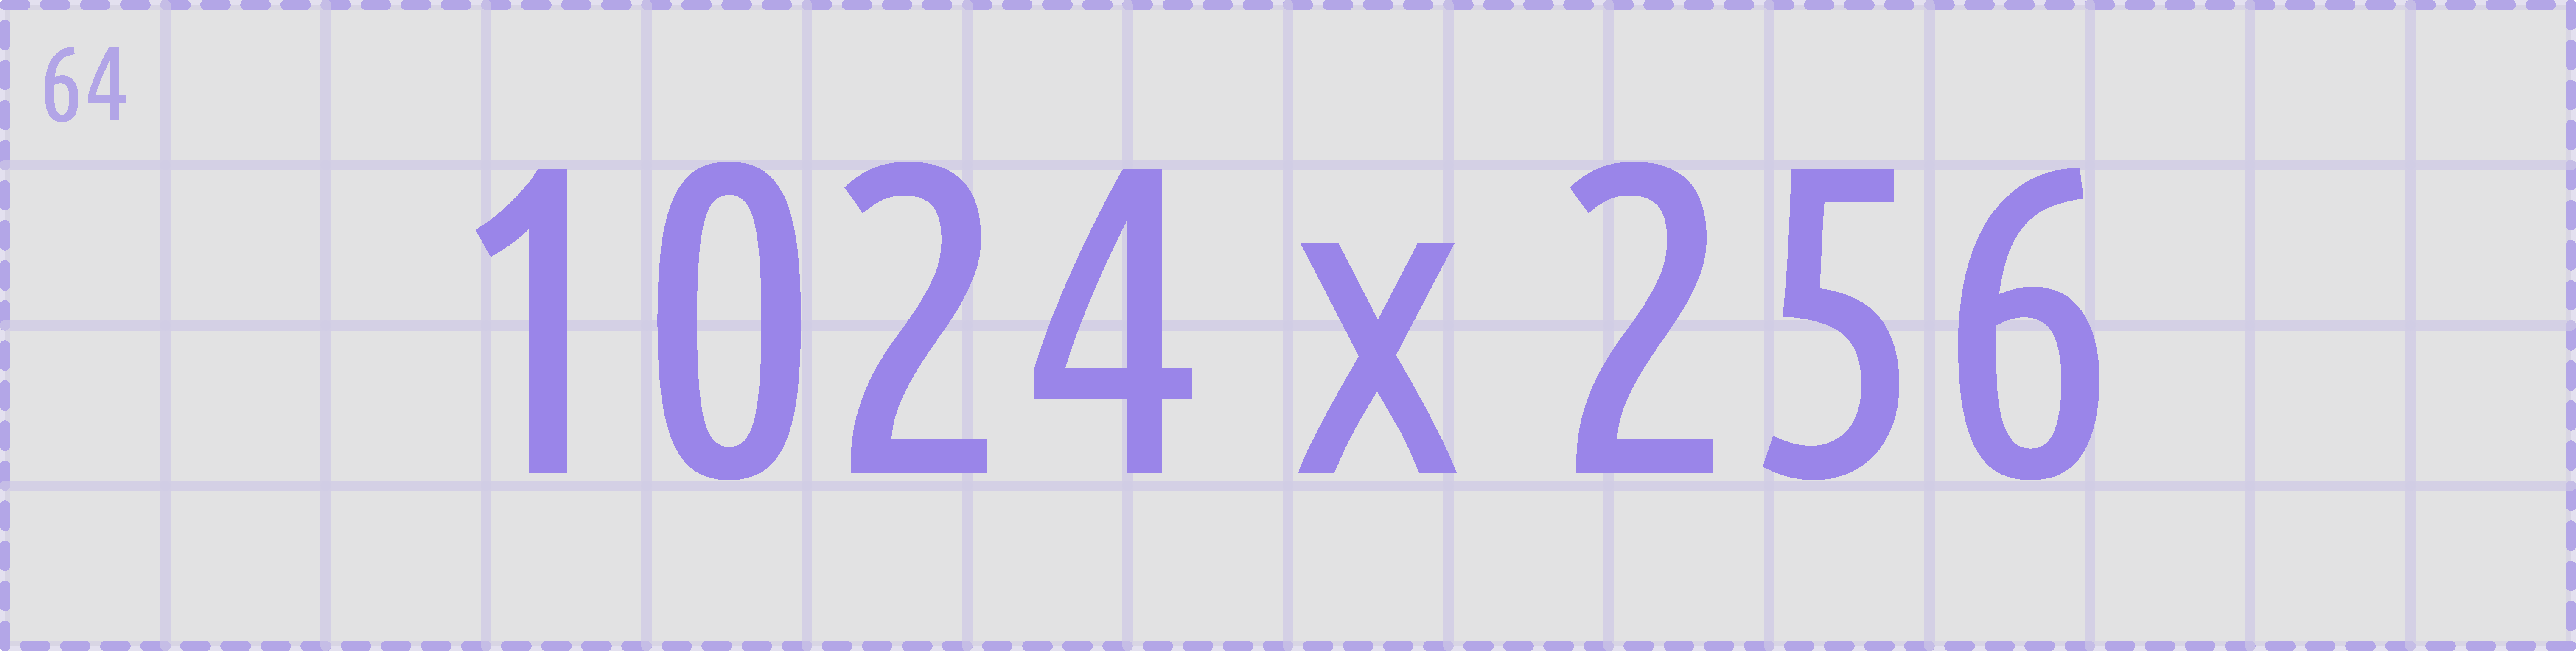
\includegraphics[width = 0.99\textwidth]{fig_1024x256.pdf}
%   \caption{Diagram of the efficient Matrix-Differential solver to compute the unknown Lagrangian entries in the model \eqref{eq:C2:dynamic_model}}
%   \vspace{-0.1cm}
%   \label{fig:C2:EX1:strain_ref}
% \end{figure}
% \begin{figure}[!t]
%  \vspace{-3mm}
%   \centering
%   \def\svgwidth{0.9\linewidth}
%   \input{./3_chapters/2_chapter/img/fig_C2_solver_diagram.pdf_tex}
%   \vspace{-0.25cm}
%   \caption{bla}
%   \vspace{-0.1cm}
%   \label{fig:C2:stiffness_model}
% \end{figure}
%
We wish to stress that $\mat{F}_1$ collects all elements related to the forward kinematics, whereas $\mat{F}_2$ contains the dynamic entities related to the Lagrangian model. Following the spatial Matrix-Differential equation in \eqref{eq:C2:MDE} above, its solution will be a matrix $\mat{Z} := \text{blkdiag}\left( \mat{Z}_1, \mat{Z}_2 \right)$ composed of two state matrices $\mat{Z}_1$ and $\mat{Z}_2$:
%
\begin{align}
\mat{Z}_1(\sigma,\q,\dq) & := \begin{pmatrix}
\begin{matrix}
\PhiB  & \gammaB \\ 0_{3\times3} &  0_{3}
\end{matrix} \;\; \vrule & \!\mat{B}_1 & \vrule & \!\mat{B}_2 \;\;\;
 \end{pmatrix}, \\[0.5em]
\mat{Z}_2(\sigma,\q,\dq) & := \begin{pmatrix} \mat{M} & \mat{C} & \mat{f}\!\grav \end{pmatrix},
\end{align}
%
Such a set of Matrix-Differentials as in \eqref{eq:C2:MDE} are not supported natively by standard ODE solvers. Therefore, an explicit second-order Runge-Kutta solver for MDEs is developed such that efficiently computes the evolution of the state matrix $\mat{Z}$ along $\Xs = [0,L]$. The numerical solver is written in \matlab \texttt{2021a} and it can be found in the public repository of \sorotoki (see implementation at \cite{SorotokiCode}).

As for state trajectories along the temporal regime $\mathbb{T} = [0,T]$, an implicit trapezoidal integration scheme is proposed to solve the approximated continuum dynamics, which are generally less conservative on discretization to preserve numerical stability. Here implicit schemes are favored over the explicit scheme since a coarser time integration can significantly increase real-time performance. In addition, to further boost the performance of the temporal integration, a cost-effective approximation of the Hessian is introduced. For more detail on the temporal integration scheme of the solver can be found in Appendix \ref{app:C2:timeint}


%%%%%%%%%%%%%%%%%%%%%%%%%%%%%%%%%%%%%%%%%%%%%%%%%%%%%%%%%%%%%%%%%%%%%%%%%%%%%%%%


% Cosserat-beam frame work
%!TEX root = ../../thesis.tex
\graphicspath{{3_chapters/3_chapter/img/}}
%%%% CHAPTER 1 *****************************************************************
\chapter[Dynamic modeling of soft robots -- Beyond PCC]{Dynamic Modeling -- Beyond \\ the Constant Strain Approach}
\label{chap: chapter 3}


\blankfootnote{This chapter is based on: {B.J. Caasenbrood, A.Y. Pogromsky, and H. Nijmijer. \textit{Energy-shaping Controllers for Soft Robot Manipulators
through Port-Hamiltonian Cosserat Models.} SN Computer Science, Springer, 2022. (under review) %\texttt{doi:} \url{10.1089/soro.2021.0035}}. 
}
\disclaimer \;Original work is found at \cite{Caasenbrood2021}. Last modified on \today.
}
%%%% ABSTRACT ******************************************************************
%!TEX root = ../../thesis.tex
\chapterabstract{
In this work, we discuss the application of energy-based controller design for under-actuated soft robot manipulators. The continuous dynamics of the soft robot are modeled through the differential geometry of Cosserat beams. Using a finite-dimensional truncation, the system can be written as a reduced port-Hamiltonian model that preserves the passivity condition. Then, a model-based controller is introduced that produces a local minimizer of closed-loop potential energy for the desired end-effector configuration. The stabilizing control utilizes an energy-based approach and exploits the passivity of soft robotic system. The effectiveness of the controller is demonstrated through extensive simulations of various soft manipulators that share a resemblance with biology.}

%%%% MAIN **********************************************************************
\ifx\printChapterTwo\undefined
\else

\section{Introduction} \label{sec:chap3_introduction}
%!TEX root = ../../thesis.tex
The field of soft robotics is slowly growing as a prominent successor to conventional rigid robotics. Contrary to rigid robots, soft robots explore `\textit{soft materials}' that significantly enhance the robot's dexterity, inherent safety, enable a rich family of motion primitives, and provide environmental robustness. By fully exploiting soft materials, soft robotics places the first steps towards achieving performance similar to biology \cite{Choi2011,Falkenhahn2015,Marchese2014}. In this work, we primarily focus on a subclass of soft robots called '\textit{soft manipulators}'.

Although significant steps have been taken towards bridging biology and soft robotics, its innate infinite-dimensionality poses substantial challenges on modeling and control. To be more specific, soft robots theoretical allow for infinitely many degrees-of-freedom along their continuously deformable body. This renders them particularly suited for PDE models \cite{Duriez2013,Largilliere2015,Wu2021} rather than the conventional ODE for traditional robotics \cite{Spong2006,Murray1994}. Additionally, their actuation often employs distributed loads (e.g., pneumatics \cite{Falkenhahn2015,Marchese2014} and tendons \cite{Till2019,Wu2021}). Consequently, classical descriptions of rigid links and joints paired with local actuation are no longer viable nor physically representative. This paradigm shift calls for novel control-oriented modeling approaches tailored for hyper-flexible and under-actuated robotic systems.

In the last decade, the field of modeling for soft robotic systems has matured sufficiently and currently their applicability in model-based control is slowly feasible \cite{DellaSantina2021}. To highlight a few: reduced-order finite element models \cite{Duriez2013,Zhang2017,Wu2021}, constant and non-constant curvature approaches \cite{Katzschmann2019,Santina2020}, Cosserat-beam models \cite{Renda2020,Boyer2021}, and learning-based approaches \cite{Bruder2019}. The Piece-wise Constant Curvature (PCC) model -- a popular method of state reduction that assumes piecewise constant strains along the soft robot's body -- has proven to be viable for modeling solution applicable to feedforward controllers \cite{Falkenhahn2015}, and more recently model-based feedback controllers \cite{Santina2020,Katzschmann2019}. Nevertheless, the PCC approach has limitations. They do not originate from continuum mechanics and thus are only applicable in restrictive settings. Although computationally performance might surpass continuous models, due to intrinsic kinematic restrictions, they are unable to capture important continuum phenomena, like buckling, environmental interaction, or wave propagation.

On the contrary, Cosserat beam-models have shown to capture a wide range of continuum deformations. Cosserat models originate from continuum mechanical PDE description and thus allow a more accurate description of the hyper-flexible nature under large deformations. The computational dynamics of Cosserat beams have been extensively developed by \cite{Simo1986} through Geometrically-Exact finite elements on the Lie group $\SE{3}$; and recently, these models are slowly gaining popularity in the soft robotics community \cite{Renda2018,Renda2020,Boyer2021,Till2019}. Ultimately, the strong nonlinearities paired with the diligence to achieve biological performance encourages Cosserat models for control. Yet, compared to PCC, literature on model-based control is scarce.

In this work, we aim to highlight the capabilities of Cosserat models for model-based control, in particular energy-based strategies. To this end, a finite-dimensional modeling approach is proposed such that the continuous dynamics can be cast into a port-Hamiltonian (pH) structure. The Lagrangian modeling framework is adopted from \cite{Boyer2021} and \cite{Renda2020}, but modified to suit a pH-structure. The main advantage of pH systems is the common formalism with energy-based control. Through the pH structure, we propose an energy-shaping control law that ensures stabilization of the end-effector of the soft robot. Similar energy-based control strategies can be found in \cite{Franco2020,Schaft2004,Ortega2002,Ortega1998} for rigid-body systems. As a study case, we consider a soft robot manipulator inspired by an octopus tentacle (see Figure 1). With the ability to deform continuously and its distributed muscular system, it is ideal for illustrating the complex morphological motions present in soft robotics. All code is made publicly available \cite{Caasenbrood2020}, and builds upon the previous work \cite{Caasenbrood2021}.

This work is organized as follows. Section \ref{sec:2} will detail a modeling approach for a general class of soft robot manipulators, starting with the Cosserat-beam theory. In Section \ref{sec:3}, we propose an energy-shaping control strategy. Lastly, we show the effectiveness of energy-based controller through numerical simulation in Section  \ref{sec:4}, followed by a brief conclusion in Section  \ref{sec:5}.


\vspace{-3mm}
\section{Generalized models for soft manipulators} \label{sec:chap3_model}
%!TEX root = ../../thesis.tex
%\subsection{Preliminaries on Lie groups}
Throughout this work, we will explore Lie group theory. We introduce the following notations: the Lie group of rigid-body transformation on $\R^3$ is denoted by $\SE{3}$, whereas the group of homogeneous rotation is denoted by $\SO{3}$. The tangent space at the identity of the group is called the Lie algebra, and it can be used to describe the evolution of the Lie group. The Lie algebra of $\SE{3}$ and $\SO{3}$ are denoted by $\seg{3}$ and $\sog{3}$, respectively. Lastly, the cross operator (\ie, "$\times$") and hat operator (\ie, "$\wedge$") are used to transform a column vector of $\R^3$ or $\R^6$ into an element of the Lie algebra $\sog{3}$ or $\seg{3}$, respectively. A comprehensive introduction is given in Appendix \ref{app:C3:liegroup} based on the work of Bullo (1995, \cite{Bullo1995}). 
%
%
% \begin{figure}[!t]
%   \vspace{-0.6mm}
%   \centering
%   \ifx\printFigures\undefined
%   \else
%   \includegraphics[width = 0.99\textwidth]{fig_C3_schematic.pdf}
%   \fi
%   \caption{Schematic representation of the Piece-wise Constant Curvature model (PCC) for general soft robotic system, given by a parameterized curve $^0 \gammaB: \Xs \times \Ts \to \R^3$ and orientation matrix $^0 \PhiB: \Xs \times \Ts \to \SO{3}$. The frame $\{\sigma\}$ is rigidly attached to $^0 \gammaB$ such that variation of $\sigma$ give insight into the differential geometry of the curve.}
%   \label{fig:C2:configuration}
% \end{figure}
% %
\begin{figure}[!t]
  \vspace{-0.6mm}
  \centering
 \includegraphics[width = 0.99\textwidth]{3_chapters/3_chapter/img/fig_C3_schematic.pdf}
  \caption{Schematic representation of the continuously variable Cosserat beam model for a general class of soft manipulators, given by a backbone $^0 \gammaB: \Xs \times \Ts \to \R^3$ and orientation matrix $^0 \PhiB: \Xs \times \Ts \to \SO{3}$. This forms a parameterized curve $\gB = (^0 \PhiB,\,^0\gammaB) \in \SE{3}$. The representation of the soft robot is inspired by the octopus' tentacle whose the muscle forces are modelled as a distributed input $\FT_u: \Xs \times \Ts \to \cose{3}$ (\ie, a co-vector belonging to the dual space of $\seg{3}$). \label{fig:C3:example1}}
  \vspace{-0.4cm}
\end{figure}
%
\subsection{Preliminary on geometric Cosserat theory}
In Cosserat theory, slender deformable solids are modeled as elastic strings subjected to geometric finite-strain theory. Drawing the analogy to soft robotics, we model the soft robot as a one-dimensional spatial curve passing through the geometric center of the soft robot (see Figure 1). Given its spatial-temporal nature, we introduce a temporal variable $t \in [0,\,T]$ with finite horizon time $T$, and a spatial variable $\sigma \in [0,\,L]$ with $L$ the undeformed length of the soft robot. For each point on the backbone, we introduce a (mobile) coordinate frame. The homogeneous rotation related to these coordinate frames is given by the rotation matrix $\mat{\Phi}: [0,L] \times [0,t] \to  \SO{3}$, and their origin by the position vector $\vec{\gamma}: [0,L] \times [0,T] \to \R^3$. For convenience and readability, we will denote the temporal and spatial domains as $\Ts = [0,\,T]$ and $\Xs = [0,\,L]$, respectively.

Following the geometric approach \cite{Simo1986,Boyer2010,Boyer2021,Renda2018,Renda2020}, we may equivalently represent each coordinate frames that are rigidly attached to the continuous backbone of the soft robot by a parameterized space curve in $\SE{3}$:
%
\begin{equation}
\mat{g}(\sigma,t) = \begin{pmatrix} \mat{\Phi}(\sigma,t) & \mat{\gamma}(\sigma,t) \\ \vec{0}_3^\top & 1 \end{pmatrix} \in \SE{3}.
\label{eq:C3:backbone}
\end{equation}
%
Now, an expression for the strain field $\vec{\xi}$ and velocity field $\vec{\eta}$ anywhere on the Cosserat beam can be found by exploring the differential geometry of the curve. To do so, we must introduce some smoothness conditions.

\begin{asm}[On differentiability]
\label{assum:1}
All control inputs acting on the continuum time-variant system, \ie, a distributed control wrench $\FT_{u}(\sigma,t)$ acting on the backbone curve \eqref{eq:C3:backbone}, are considered to be sufficiently smooth for any instance $t \in \Ts$ and $\sigma \in \Xs$ such that parametrized backbone $\mat{g}(\sigma,t) \in \SE{3}$ is everywhere differentiable on $\Xs$ and $\Ts$.
\end{asm}

\newpage
\subsection{Local strain and velocity}
Following the works of Boyer et al. (2021, \cite{Boyer2021}) and Renda et al. (2020, \cite{Renda2018,Renda2020}), let $\vec{\Gamma} = (\kappa_1,\, \kappa_2, \kappa_3)^\top$ and $\vec{U} = (\nu_1,\, \nu_2,\, \nu_3)^\top$ be the torsion-curvature and elongation-shear strain vector, respectively. Then, an expression for strain field $\vec{\xi}(\sigma,t)$ is obtained through spatial differentiation of $\mat{g}$:
%
\begin{equation}
\hat{\vec{\xi}} := \mat{g}\inv \frac{\p \mat{g}}{\p \sigma} = \begin{pmatrix} \vec{\Gamma}^\times & \vec{U} \\[0.5em] \vec{0}_3^\top & 0 \end{pmatrix} \;\; \Longrightarrow \;\; \vec{\xi} := \begin{pmatrix} \vec{\Gamma} \\ \vec{U} \end{pmatrix}.
\label{eq:C3:xi}
\end{equation}
%
Similarly, let $\vec{\Omega} = (\omega_1, \omega_2, \omega_3)^\top$ and $\vec{V} = (v_1,\,v_2,\, v_3)^\top$ be the angular and linear velocity vector, respectively. Then, an expression for velocity field $\vec{\eta}(\sigma,t)$ is obtained through time differentiation of $\vec{g}$:
%
\begin{equation}
\hat{\vec{\eta}} := \mat{g}\inv \frac{\p \mat{g}}{\p t} = \begin{pmatrix} \vec{\Omega}^\times & \vec{V} \\[0.5em] \vec{0}_3^\top & 0 \end{pmatrix} \;\; \Longrightarrow \;\; \vec{\eta} := \begin{pmatrix} \vec{\Omega} \\ \vec{V} \end{pmatrix}.
\label{eq:C3:eta}
\end{equation}
%
Let it be clear to the reader that $\xiB(\sigma,t)$ and $\etaB(\sigma,t)$ are yet unknown vector fields, which simply follow from the differential geometry of $\SE{3}$, and thus they live in its tangent space $\seg{3}$ -- called its Lie algebra. Now given this geometric structure, we can start detailing the forward kinematics of the soft robot by exploring the smoothness in both space and time of the parameterized curve $\gB(\sigma,t)$. 

Recalling Assumption \ref{assum:1}, which assumes the configuration space $\mat{g}$ to be everywhere differentiable, we can introduce the equality of mixed partials, \ie, $\frac{\p }{\p t}(\frac{\p \mat{g}}{\p \sigma}) = \frac{\p }{\p \sigma} (\frac{\p \mat{g}}{\p t})$. Then, by substitution of $\frac{\p \mat{g}}{\p t} = \vec{g}\hat{\vec{\eta}}$ and $\frac{\p \mat{g}}{\p \sigma} = \mat{g}\hat{\vec{\xi}}$, we obtain the so-called \emph{compatibility equation}:
%
\begin{equation}
\mat{g} \hat{\vec{\eta}}\hat{\vec{\xi}} + \mat{g} \frac{\p \hat{\vec{\xi}}}{\p t}  = \mat{g} \hat{\vec{\xi}} \hat{\vec{\eta}}  + \mat{g} \frac{\p \hat{\vec{\eta}}}{\p \sigma},
\label{eq:C3:compatibility}
\end{equation}
%
\noindent which can be regarded as an equality constraint that follows from the smoothness of the group (or manifold) in both space and time. Pre-multiplying the expression above with $\mat{g} \inv \in \SE{3}$ and rearranging the equality, we obtain
%
\begin{equation}
\frac{\p \hat{\vec{\eta}}}{\p \sigma} = -\left(\hat{\vec{\xi}}\hat{\vec{\eta}} - \hat{\vec{\eta}}\hat{\vec{\xi}} \right) + \dot{\hat{\vec{\xi}}}.
\end{equation}
%
\noindent Focusing on the RHS term $(\hat{\vec{\xi}}\hat{\vec{\eta}} - \hat{\vec{\eta}}\hat{\vec{\xi}})$, we can recognize the Lie bracket or the commuter between the geometric vector fields $\vec{\xi}$ and $\vec{\eta}$ (see \cite{Murray1994}). Since the Lie bracket $[\hat{\vec{\xi}},\hat{\vec{\eta}}]$ itself also belongs to Lie algebra $\seg{3}$, which is isomorphic to $\R^6$ via the operator $\hat{\vec{\eta}} \to \vec{\eta}$, we can rewrite the expressions as follows
%
\begin{equation}
\frac{\p \vec{\eta}}{\p \sigma} = -\ad_{\vec{\xi}}\vec{\eta} + \dot{\vec{\xi}},
\label{eq:C3:pde_kin}
\end{equation}
%
\noindent where $\ad_{(\cdot)}: \R^6 \to \R^{6\times 6}$ defines the adjoint action on vectors belonging to the Lie algebra $\seg{3}$. %The approach provided above is analogous to works \cite{Boyer2021,Renda2020,Till2019}. 
Drawing an analogy to rigid robotics, the expression in \eqref{eq:C3:pde_kin} may be seen as the forward velocity kinematics for a serial chain robot manipulator with infinitely many links. To that end, we reformulate \eqref{eq:C3:xi}, \eqref{eq:C3:pde_kin} and the time derivative of \eqref{eq:C3:pde_kin} (\ie, the acceleration) as a system of PDEs describing the full continuum-body kinematics of the continuum body:
%
\begin{equation}
\frac{\p }{\p \sigma} 
\begin{pmatrix}
\,\gB\; \\[0.25em]
\,\etaB\; \\[0.25em]
\;\dot{\etaB}\;\;
\end{pmatrix}  = 
\begin{pmatrix}
\gB \hat{\xiB} \\[0.25em]
-\ad_{\vec{\xi}}\vec{\eta} + \dot{\vec{\xi}} \\[0.25em]
-\ad_{\vec{\xi}}\dot{\etaB} -\ad_{\dot{\xiB}}\etaB  + \ddot{\vec{\xi}}
\end{pmatrix}.
\label{eq:C3:cont_kin_pde}
\end{equation}

\noindent For a general case, the boundary conditions of PDE in \eqref{eq:C3:cont_kin_pde} should satisfy $\gB(0,t) = \gB_0$, $\etaB(0,t) = \etaB_0$ and $\dot{\etaB}(0,t) = \dot{\etaB}_0$. However, in case of a manipulator whose base is spatially fixed, the boundary conditions should satisfy $\gB(0,t) = g_0$, and $\etaB(0,t) = \dot{\etaB}(0,t) = \vec{0}_6$. Notice that if the strain fields $\xiB$, $\dot{\xiB}$, and $\ddot{\xiB}$ are known, the partial differential equation in \eqref{eq:C3:cont_kin_pde} can simply be treated as a system of ODEs, which can be easily solved using numerical approaches.
% %
% Since we assume the $\mat{g}$ to be everywhere differentiable, we can derive a PDE for the continuous forward kinematics of the soft robot \cite{Boyer2021,Renda2020}:
% %
% \begin{equation}
% \dfrac{\p \vec{\eta}}{\p \sigma} = -\textbf{ad}_{\vec{\xi}} \vec{\eta} + \dot{\vec{\xi}},
% \label{eq:pde_kin}
% \end{equation}
% %
% where $\ad_{(\cdot)}$ denotes the adjoint action on the Lie algebra (full derivation in Appendix A). Drawing an analogy to rigid robotics, the expression in \eqref{eq:pde_kin} may be seen as the forward velocity kinematics for a serial chain robot manipulator with infinitely many links.

%%%%%%%%%%%%%%%%%%%%%%%%%%%%%%%%%%%%%%%%%%%%%%%%%%
\subsection{Finite-dimensional projection}
Similar to finite element methods, we wish to find a finite-dimensional approximation of the strain field $\vec{\xi}(\sigma,t)$ for all points on the material domain $\Xs$. To do so, we assume the following:
%
\begin{asm}
\vspace{1mm}
Assuming the strain field has a separable spatio-temporal nature, any entry of the strain vector field $\vec{\xi} = \left( \xi_1, \xi_2, ..., \xi_6 \right)^\top$ can be written as an infinite expansion of the following form:
%
\begin{equation}
\xi_i(\sigma,t) = \sum_{n=1}^\infty \theta_{n}(\sigma)q_{i,n}(t) + \xi^\circ_{i}(\sigma) \quad i\in\{1,\hdots,6\},
\label{eq:infinite_expans}
\end{equation}
%
where $\{\theta_{n}\}^\infty_{n=1}$ is the set of (orthogonal) basis functions $\theta_{n}: \Xs \to \R$ together with modal coefficients $q_{i,n}: \Ts \to \R$, and an intrinsic time-invariant strain $\xi^\circ_{i}: \Xs \to \R$. The basis functions $\theta_{n}(\cdot)$ and the modal coefficients $q_n(\cdot)$ are both smooth functions.
\end{asm}

\begin{asm}
Given infinite expansion \eqref{eq:infinite_expans}, the $k$-th order truncation for any entry of the strain field, defined as
%
\begin{equation}
[\xi_i]_k(\sigma,t) := \sum_{n=1}^k \theta_n(\sigma)q_{i,n}(t) + \xi^\circ_{i}(\sigma) \quad i\in\{1,\hdots,6\},
\end{equation}
%
converges uniformly on $\Xs$ and $\Ts$ as the index $k \to \infty$. Moreover, we assume that uniform convergence holds for its partial derivatives $\tfrac{\p}{\p t} [\vec{\xi}]_k$ and $\tfrac{\p}{\p \sigma} [\vec{\xi}]_k$.
\end{asm}

\noindent Accordingly, we can rewrite the $k$-th order truncation of the complete strain field as a linear matrix operation as follows
%
\begin{align}
[\vec{\xi}]_k  & = \left(\vec{I}_6  \otimes \begin{bmatrix} \theta_1 & \hdots & \theta_k \end{bmatrix} \right) \vec{q} + \vec{\xi}^\circ,  \\[0.5em]
& =
\begingroup % keep the change local
\setlength\arraycolsep{2.5pt}
\underbrace{\begin{pmatrix}
\theta_1 & \hdots & \theta_k & \hdots & 0 & \cdots&  0 \\
\vdots & \ddots & \vdots & \ddots & \vdots & \vdots & \vdots \\
0 & \cdots&  0 & \hdots & \theta_1 & \hdots & \theta_k\end{pmatrix}}_{{\mat{\Theta}(\sigma)}}
\endgroup
\underbrace{\begin{pmatrix} q_{1,1} \\ \vdots \\ q_{6,k}\end{pmatrix}}_{\vec{q}(t)} + \vec{\xi}^\circ,
\label{eq:trunc_2}
%\vspace{-4mm}
\end{align}
%
where $\mat{\Theta} \in \R^{6 \times 6k}$ is a sparse matrix-valued function whose columns are mutually orthonormal, the operator $\otimes$ denotes the Kronecker product, and the vector $\vec{q} \in \R^{6k}$ the collection of all time-variant modal coefficients related to the columns of $\mat{\Theta}$. Although a wide variety of bases are possible (see for instance \cite{Boyer2021,DellaSantina2020}), we have chosen a modified Legendre polynomial set:
%
\begin{figure}[!t]
  \vspace{-3mm}
    %\centering
    %\ifx\printFigures\undefined
    %\else$$
    \hspace{0.7mm}
    % This file was created by matlab2tikz.
%
\definecolor{mycolor1}{rgb}{0.00000,0.34510,0.65882}%
\definecolor{mycolor2}{rgb}{0.79216,0.11765,0.17255}%
\definecolor{mycolor3}{rgb}{0.20392,0.65490,0.24706}%
\definecolor{mycolor4}{rgb}{0.93333,0.43922,0.13725}%
%
\begin{tikzpicture}

\begin{axis}[%
width=0.37\textwidth,
height=0.175\textwidth,
at={(0\textwidth,0\textwidth)},
scale only axis,
xmin=0,
xmax=1,
xtick={0,0.25,0.5,0.75,1},
xticklabels={{},{},{},{},{}},
ymin=-0.25,
ymax=1.25,
ylabel style={font=\color{white!15!black}},
ylabel={$\theta_n(\sigma)$},
axis background/.style={fill=white},
title style={font=\bfseries},
% title={$(a)$},
xmajorgrids,
ymajorgrids,
ylabel style={yshift=-2.5pt}
]
\addplot [color=mycolor1, line width=1.5pt, forget plot]
  table[row sep=crcr]{%
0	1\\
0.249249249249249	1\\
0.25025025025025	0\\
1	0\\
};
\addplot [color=mycolor2, line width=1.5pt, forget plot]
  table[row sep=crcr]{%
0	0\\
0.249249249249249	0\\
0.25025025025025	1\\
0.499499499499499	1\\
0.500500500500501	0\\
1	0\\
};
\addplot [color=mycolor3, line width=1.5pt, forget plot]
  table[row sep=crcr]{%
0	0\\
0.499499499499499	0\\
0.500500500500501	1\\
0.74974974974975	1\\
0.750750750750751	0\\
1	0\\
};
\addplot [color=mycolor4, line width=1.5pt, forget plot]
  table[row sep=crcr]{%
0	0\\
0.74974974974975	0\\
0.750750750750751	1\\
1	1\\
};
\end{axis}

\begin{axis}[%
width=0.37\textwidth,
height=0.175\textwidth,
at={(0.486\textwidth,0\textwidth)},
scale only axis,
xmin=0,
xmax=1,
xtick={0,0.25,0.5,0.75,1},
xticklabels={{},{},{},{},{}},
ymin=-1.5,
ymax=1.5,
ylabel style={font=\color{white!15!black}},
ylabel={$\theta_n(\sigma)$},
axis background/.style={fill=white},
title style={font=\bfseries},
%title={$(b)$},
xmajorgrids,
ymajorgrids,
ylabel style={yshift=-2.5pt}
]
\addplot [color=mycolor1, line width=1.5pt, forget plot]
  table[row sep=crcr]{%
0	1\\
1	1\\
};
\addplot [color=mycolor2, line width=1.5pt, forget plot]
  table[row sep=crcr]{%
0	-1\\
1	1\\
};
\addplot [color=mycolor3, line width=1.5pt, forget plot]
  table[row sep=crcr]{%
0	1\\
0.0310310310310311	0.819591363134907\\
0.0610610610610611	0.656004352701049\\
0.0900900900900901	0.508156805454103\\
0.118118118118118	0.375002630257885\\
0.145145145145145	0.255531808084361\\
0.171171171171171	0.148770392013635\\
0.196196196196196	0.0537805072339606\\
0.22022022022022	-0.0303396489582677\\
0.243243243243243	-0.10445580715851\\
0.265265265265265	-0.169397625854082\\
0.286286286286286	-0.225958691424157\\
0.307307307307307	-0.277217157097037\\
0.327327327327327	-0.321104888672456\\
0.346346346346346	-0.358343328313298\\
0.364364364364364	-0.389617846074302\\
0.381381381381381	-0.415577739902064\\
0.397397397397397	-0.436836235635034\\
0.413413413413414	-0.455016578139701\\
0.428428428428429	-0.469265060856652\\
0.442442442442442	-0.480122765408051\\
0.456456456456456	-0.488623758894029\\
0.469469469469469	-0.494407320233146\\
0.482482482482482	-0.498158819480141\\
0.495495495495496	-0.499878256635014\\
0.507507507507508	-0.499661823986148\\
0.519519519519519	-0.497713930146363\\
0.532532532532533	-0.493649805962118\\
0.545545545545546	-0.487553619685752\\
0.558558558558559	-0.479425371317263\\
0.572572572572573	-0.468399330261192\\
0.586586586586587	-0.455016578139701\\
0.601601601601602	-0.438062687311937\\
0.617617617617618	-0.416996576155735\\
0.633633633633634	-0.392852311771231\\
0.650650650650651	-0.363826288751214\\
0.668668668668669	-0.329305281257233\\
0.687687687687688	-0.288639991342694\\
0.707707707707708	-0.241145048952857\\
0.727727727727728	-0.188840492143795\\
0.748748748748749	-0.128744359975591\\
0.770770770770771	-0.0600991381772165\\
0.793793793793794	0.0178887596305013\\
0.817817817817818	0.106048991934878\\
0.842842842842843	0.205247289331373\\
0.868868868868869	0.316385454523592\\
0.894894894894895	0.435651868084301\\
0.921921921921922	0.56810864918973\\
0.94994994994995	0.714729744759775\\
0.978978978978979	0.876525173822471\\
1	1\\
};
\addplot [color=mycolor4, line width=1.5pt, forget plot]
  table[row sep=crcr]{%
0	-1\\
0.0190190190190189	-0.782485871940692\\
0.0380380380380381	-0.585849574761409\\
0.0560560560560561	-0.418072891875022\\
0.0740740740740742	-0.267591322461007\\
0.0910910910910911	-0.14071778835241\\
0.107107107107107	-0.0342981766697772\\
0.123123123123123	0.0600275897464979\\
0.138138138138138	0.137912741624562\\
0.153153153153153	0.206008053341874\\
0.167167167167167	0.26108942025359\\
0.18018018018018	0.305205863277448\\
0.193193193193193	0.342823368979655\\
0.205205205205205	0.372007618203764\\
0.216216216216216	0.394270823050955\\
0.227227227227227	0.412405233898399\\
0.237237237237237	0.425443028180901\\
0.246246246246246	0.434472266818126\\
0.255255255255255	0.441030078586554\\
0.264264264264264	0.445204206451941\\
0.272272272272272	0.446984357566612\\
0.28028028028028	0.447012056580584\\
0.288288288288288	0.445348928183114\\
0.297297297297297	0.441533571555485\\
0.306306306306306	0.435743998198344\\
0.316316316316316	0.427102419377978\\
0.327327327327327	0.41505036134801\\
0.339339339339339	0.399043011303921\\
0.352352352352352	0.378569076902044\\
0.367367367367367	0.351233983600084\\
0.383383383383384	0.318131447265587\\
0.401401401401401	0.276624908126279\\
0.422422422422422	0.223395060218871\\
0.447447447447447	0.154754895576799\\
0.481481481481481	0.0554285423969925\\
0.55955955955956	-0.174453117166602\\
0.585585585585586	-0.244218652545899\\
0.606606606606607	-0.295588205146412\\
0.625625625625626	-0.337224912399687\\
0.641641641641642	-0.368091627977139\\
0.656656656656657	-0.393078784510256\\
0.66966966966967	-0.411320689517806\\
0.681681681681682	-0.42510521776274\\
0.692692692692693	-0.434982658462395\\
0.702702702702703	-0.441533571555485\\
0.711711711711712	-0.445348928183114\\
0.720720720720721	-0.447102325115474\\
0.728728728728729	-0.446858939689107\\
0.736736736736737	-0.444855399075886\\
0.744744744744745	-0.441030078586554\\
0.753753753753754	-0.434472266818126\\
0.762762762762763	-0.425443028180901\\
0.771771771771772	-0.413854619709123\\
0.781781781781782	-0.3978703949716\\
0.792792792792793	-0.376369795653945\\
0.803803803803804	-0.350609329511154\\
0.815815815815816	-0.317460398130658\\
0.827827827827828	-0.278843238464521\\
0.840840840840841	-0.230596015489016\\
0.854854854854855	-0.170884130911225\\
0.868868868868869	-0.10280934270289\\
0.883883883883884	-0.020216582116821\\
0.898898898898899	0.0727618041999487\\
0.914914914914915	0.183843708779055\\
0.931931931931932	0.315873496183937\\
0.948948948948949	0.462912686785208\\
0.966966966966967	0.635618141204809\\
0.984984984984985	0.826515637191178\\
1	1\\
};
\end{axis}
\end{tikzpicture}%
  
    % This file was created by matlab2tikz.
%
\definecolor{mycolor1}{rgb}{0.00000,0.34510,0.65882}%
\definecolor{mycolor2}{rgb}{0.79216,0.11765,0.17255}%
\definecolor{mycolor3}{rgb}{0.20392,0.65490,0.24706}%
\definecolor{mycolor4}{rgb}{0.93333,0.43922,0.13725}%
%
\begin{tikzpicture}

\begin{axis}[%
width=0.37\textwidth,
height=0.175\textwidth,
at={(0\textwidth,0\textwidth)},
scale only axis,
xmin=0,
xmax=1,
xtick={0,0.25,0.5,0.75,1},
xticklabels={{0},{},{},{},{$L$}},
ytick={-1,0,1},
yticklabels={{$-\infty$},0,{$+\infty$}},
xlabel style={font=\color{white!15!black}},
xlabel={space $\sigma$},
ymin=-1.2,
ymax=1.2,
ylabel style={font=\color{white!15!black}},
ylabel={$\p \theta_n/\p \sigma (\sigma)$},
axis background/.style={fill=white},
xmajorgrids,
ymajorgrids,
ylabel style={yshift=-2.5pt}
]
\addplot [color=mycolor1, line width=1.5pt, forget plot]
  table[row sep=crcr]{%
0.00100100100100109	0\\
0.249249249249249	0\\
0.25025025025025	-1\\
0.251251251251251	0\\
1	0\\
};
\addplot [color=mycolor2, line width=1.5pt, forget plot]
  table[row sep=crcr]{%
0.00100100100100109	0\\
0.249249249249249	0\\
0.25025025025025	1\\
0.251251251251251	0\\
0.499499499499499	0\\
0.500500500500501	-1\\
0.501501501501502	0\\
1	0\\
};
\addplot [color=mycolor3, line width=1.5pt, forget plot]
  table[row sep=crcr]{%
0.00100100100100109	0\\
0.499499499499499	0\\
0.500500500500501	1\\
0.501501501501502	0\\
0.74974974974975	0\\
0.750750750750751	-1\\
0.751751751751752	0\\
1	0\\
};
\addplot [color=mycolor4, line width=1.5pt, forget plot]
  table[row sep=crcr]{%
0.00100100100100109	0\\
0.74974974974975	0\\
0.750750750750751	1\\
0.751751751751752	0\\
1	0\\
};
\end{axis}

\begin{axis}[%
width=0.37\textwidth,
height=0.164\textwidth,
at={(0.486\textwidth,0.011\textwidth)},
scale only axis,
xmin=0,
xmax=1,
xtick={0,0.25,0.5,0.75,1},
xticklabels={{0},{},{},{},{$L$}},
xlabel style={font=\color{white!15!black}},
xlabel={space $\sigma$},
ymin=-0.01,
ymax=0.015,
ylabel style={font=\color{white!15!black}},
ylabel={$\p \theta_n/\p \sigma(\sigma)$},
axis background/.style={fill=white},
xmajorgrids,
ymajorgrids,
ylabel style={yshift=-2.5pt}
]
\addplot [color=mycolor1, line width=1.5pt, forget plot]
  table[row sep=crcr]{%
0.00100100100100109	0\\
1	0\\
};
\addplot [color=mycolor2, line width=1.5pt, forget plot]
  table[row sep=crcr]{%
0.00100100100100109	0.00200200200200196\\
1	0.00200200200200196\\
};
\addplot [color=mycolor3, line width=1.5pt, forget plot]
  table[row sep=crcr]{%
0.00100100100100109	-0.00599999398798179\\
1	0.00599999398798179\\
};
\addplot [color=mycolor4, line width=1.5pt, forget plot]
  table[row sep=crcr]{%
0.00100100100100109	0.0119819719820118\\
0.037037037037037	0.00989780573368138\\
0.0730730730730731	0.00796962698002934\\
0.109109109109109	0.00619743572105302\\
0.145145145145145	0.00458123195675597\\
0.181181181181181	0.00312101568713552\\
0.217217217217217	0.00181678691219256\\
0.253253253253253	0.000668545631927309\\
0.289289289289289	-0.000323708153660229\\
0.325325325325325	-0.00115997444457028\\
0.361361361361361	-0.00184025324080306\\
0.397397397397397	-0.0023645445423579\\
0.433433433433434	-0.00273284834923548\\
0.469469469469469	-0.00294516466143557\\
0.505505505505506	-0.00300149347895817\\
0.541541541541542	-0.00290183480180284\\
0.577577577577578	-0.00264618862997024\\
0.613613613613614	-0.00223455496346037\\
0.64964964964965	-0.00166693380227234\\
0.685685685685686	-0.000943325146407048\\
0.721721721721722	-6.37289958642651e-05\\
0.757757757757758	0.000971854649356008\\
0.793793793793794	0.00216342578925377\\
0.82982982982983	0.00351098442382924\\
0.865865865865866	0.00501453055308221\\
0.901901901901902	0.00667406417701244\\
0.937937937937938	0.00848958529562016\\
0.973973973973974	0.0104610939089056\\
1	0.0119819719820118\\
};
\end{axis}
\end{tikzpicture}%
    %\fi
    \vspace{-3mm}
    \caption{Example plot of the Constant-Strain parameterization in Chapter 3 $(a)$, and the new strain parameterization \eqref{eq:C3:chebyshev} using Chebyshev polynomials $(b)$. The ordering of the strain basis is as follows $\{\theta_1,...,\theta_4\} = \{\ldata{Matlab1},\ldata{Matlab2},\ldata{Matlab3},\ldata{Matlab4}\}$. Notice that the discontinuities in the PCC models induce spikes that directly violate the compatibility equation in \eqref{eq:C3:compatibility}.}
    \label{fig:C4:basis_example}
  \end{figure}
  %
\begin{equation}
\theta_n(\sigma) = \dfrac{2}{2^{n}(n-1)!} \dfrac{d^{n-1}}{d\sigma^{n-1}}\left[\left( \dfrac{2\sigma}{L}-1 \right)^2 -1 \right]^{n-1}
\label{eq:C3:chebyshev}
\end{equation}
%
\noindent with $n \in \Z/\{0\}$ the polynomial degree. A comparison between the proposed basis and previous method in Chapter 3 is shown in Figure \ref{fig:C4:basis_example}. Please note now that the inner product between elements of the set of modified Legendre functionals $\{\theta_n\}_{n = 1}^k$ satisfies $\inner{\theta_i}{\theta_j}_{\Xs} := \int_\Xs{\theta_i}{\theta_j} d\sigma = 0$ for $i \neq j$, and $1$ otherwise. An alternative option could be constructing the set of basis functions through the so-called '\textit{snapshot decomposition method}' using FEM-driven data \cite{Astrid2008,Duriez2013,Largilliere2015}.

\begin{rmk}
The idea of joint parameterization by investigating the relation between material and structural topology of the soft robot is explored in Chapter 5.
\end{rmk}

\subsection{Reduced-order curve kinematics}
Given the finite-dimensional truncation in \eqref{eq:trunc_2}, we can now find an expression for the finite-dimensional forward kinematics in terms of the generalized coordinates $\vec{q}$ and its velocities components $\dot{\vec{q}}$.

First, let us regard the configuration of the soft robot $\mat{g} \in \SE{3}$. Recall that the spatial evolution of the curve is described by $\p \mat{g}/\p\sigma = \mat{g} \vec{\xi}^\wedge$, see Eq. \eqref{eq:C3:xi}. Given the initial condition $\mat{g}(0,\cdot) = \mat{g}_0$, an approximation of the continuously deformable soft robot can be obtained by partial integration over the spatial domain:
%
\vspace{-2mm}
\begin{equation}
[\mat{g}]_k(\sigma,\vec{q}) = \mat{g}_0 \exp_{\SE{3}}\left[\int_0^\sigma [\hat{\vec{\xi}}]_k(s,\vec{q}) \; ds \right].
\end{equation}
%
The computation of the mapping $\exp_{\SE{3}}$ is given in Appendix \ref{app:C3:liegroup}. Please note that this nothing more than the reconstruction of the curve by integration of its tangent space along its spatial parameter $\sigma$. Next, lets regard the velocity kinematics $\vec{\eta}(\sigma,t)$ for any point $\sigma$ on the backbone curve. Using the differential property of the adjoint action $\mat{\ad}_{\vec{\xi}} = -\p /\p \sigma [\Ad_{g^{-1}}] \Ad_{g}$ \cite{Murray1994}, we can rewrite the continuous forward kinematics in \eqref{eq:C3:pde_kin} as
%
\begin{equation}
\frac{\p \vec{\eta}}{\p \sigma } = \frac{\p }{\p \sigma }\left(\mat{\Ad}_{\mat{g}^{-1}}\right) \mat{\Ad}_{\mat{g}} \vec{\eta} + \dot{\vec{\xi}}. \label{eq:eta_adg}
\end{equation}
%
Now, given the initial condition $\vec{\eta}(0,t) = \vec{0}_6$ and the approximations $[\vec{\xi}]_k$ and $[\mat{g}]_k$, we can find an approximation to the velocity twist $\vec{\eta}$ by partial integration over space:
%
\begin{equation}
[\vec{\eta}]_k(\sigma,\vec{q},\dot{\vec{q}}) = \Ad_{[\mat{g}]_k}\inv \int_0^\sigma \Ad_{[\mat{g}]_k} \mat{\Theta} \; ds \,\dot{\vec{q}} := [\mat{J}]_k\, \dot{\vec{q}}, \label{eq:C3:eta_analytic}
\end{equation}
%
which naturally gives rise to the geometric Jacobian $[\mat{J}]_k \in \R^{6\times 6k}$. The geometric Jacobian plays an important role in obtaining the Lagrangian form of the reduced-order dynamic model. Finally, to express the acceleration twist, we take the time-derivative of \eqref{eq:C3:eta_analytic} leading to
%
\begin{align}{}
[\dot{\vec{\eta}}]_k & = [\mat{J}]_k\ddot{\vec{q}} + \dot{[\mat{J}]}_k\dot{\vec{q}}, \notag \\
& = [\mat{J}]_k\ddot{\vec{q}} + \Ad_{[\mat{g}]_k}\inv \int_0^\sigma \Ad_{[\mat{g}]_k} \ad_{[\vec{\eta}]_k} \mat{\Theta} \; ds \,\dot{q} \label{eq:C3:deta_analytic},
\end{align}
%
which gives rise to the analytic expression of the time-derivative of the geometric Jacobian $\dot{[\mat{J}]}_k$ (see Appendix \ref{app:C3:jacobian} for the derivation).

\subsection{Reduced-order curve dynamics using Newton-Euler}
Here, we detail the dynamics of the Cosserat beam. A majority of the dynamic framework presented here is adopted from Boyer et al. (2021, \cite{Boyer2021}); yet we introduce some modification to allow a pH-structure. First, let us consider an infinitesimal slice of continuum body that is perpendicular to the backbone curve. The kinetic momenta of this infinitesimal slice is then given by $\vec{\mu}(\sigma,t) := \MT \vec{\eta}(\sigma,t)$ in which $\MT \in \cose{3} \times \seg{3} \cong \R^{6\times 6}$ denotes the symmetric inertia tensor.
%
\begin{rmk}
For some soft robots, the inertia tensor $\MT$ may have an explicit dependency on space or time (or both). Nevertheless, for sake of simplicity, we limit ourselves to a diagonal invariant inertia tensor:
%
\begin{equation*}
\MT(\sigma,t) \cong \MT = \begin{pmatrix} \rho_0 \ten{J}  & \vec{0}_{3\times3}  \\[0.35em]
  \vec{0}_{3\times3} & \rho_0\, A\mat{I}_3 \end{pmatrix} \succ 0,
\end{equation*}
%
in which the (cross-sectional average) density is $\rho_0 > 0$, the cross-sectional area of the soft robot by $A>0$, and the second moment of area $\mat{\mathcal{J}} \in \coso{3} \times \sog{3} \cong \R^{3\times 3}$.
\end{rmk}
%
\noindent Using the expression of the kinetic momenta $\muB(\sigma,t)$ of the infinitesimal rigid body in free-motion, we can write the equation of motion for a particular slice at $\sigma$ using the Newton-Euler equations:
%
\begin{equation}
\frac{\p }{\p t} (\Ad_{\gB}^{-\top} \vec{\mu}) = \Ad_{g}^{-\top}\ten{F},\label{eq:C3:newton_euler}
\end{equation}
%
where again $\Ad_{(\cdot)}$ stands for the adjoint action, and $\ten{F} = \ten{F}_c  + \ten{F}_u - \ten{F}\grav - \ten{F}\elastic$ the resultant wrench that is composed of the constraint wrench $\ten{F}_c$, the input wrench $\ten{F}_u$, and the potential wrenches due to gravity and visco-elasticity, $\ten{F}\grav$ and $\ten{F}\elastic$, respectively. Further evaluation of \eqref{eq:C3:newton_euler} leads to
%
\begin{equation}
\MT\dot{\vec{\eta}} - \ad_{\vec{\eta}}^\top \MT \vec{\eta} = \ten{F},
\label{eq:C3:newton-euler-2}
\end{equation}
%
where we used the fact that $\dot{\Ad}_{\vec{g}} \inv = -\ad_{\vec{\eta}} {\Ad}_{\vec{g} \inv}$. Before continuing, we introduce a slight modification to the relation above. Using the fact that $\ad_{\vec{\eta}} \vec{\eta} = \vec{0}_6$, we can introduce the vector
$\ten{M} \ad_{\vec{\eta}} \vec{\eta}$ to \eqref{eq:C3:newton-euler-2} without affecting the dynamics. The importance of this modification originates from the preservation of passivity in the Lagrangian model, which is an important property in stability theorems for robotics. By substitution of the null vector, the equation of motion becomes
%
\begin{equation}
  \MT \dot{\vec{\eta}} + \left(\MT \ad_{\vec{\eta}}  - \ad_{\vec{\eta}} ^\top \MT \right) \vec{\eta} = \FT,
  \label{eq:C3:newton-euler-3}
\end{equation}
%
which is nothing more than the Newton-Euler equation for rigid-body motion on $\R^3$. To introduce the (reduced-order) Cosserat kinematics and make the expression symmetric, we substitute \eqref{eq:C3:eta_analytic} and \eqref{eq:C3:deta_analytic} into \eqref{eq:C3:newton-euler-3} and pre-multiply by $[\JB]_k^\top$:
%
\begin{multline}
  [\vec{J}]_k^\top \left( \MT [\mat{J}]_k \ddot{\vec{q}} + \MT [\dJB]_k\dot{\vec{q}} + \CT_{[\vec{\eta}]_k }\dot{\vec{q}}\right) = [\mat{J}]_k^\top \left(\FT_u - \FT\grav - \FT\elastic \right),
  \label{eq:C3:projected_NE_jacobian}
\end{multline}
%
where $\CT_{(\cdot)} = -\CT_{(\cdot)} ^\top :=  \MT \ad_{(\cdot)}  - \ad_{(\cdot)} ^\top \MT$ is a skew-symmetric matrix. It is important to note that by pre-multiplication of the transpose Jacobian, we have eliminated the constraint wrenches, \ie, $[\JB]_k^\top \FT_c = \vec{0}_n$ \cite{Murray1994}. Finally, the finite-dimensional dynamics of the deformable soft robot is found by spatial integration of \eqref{eq:C3:projected_NE_jacobian} over the material domain $\Xs$. The overall dynamics can be written in familiar Euler-Lagrangian (EL) form as follows
%
\begin{equation}
  \mat{M}(\vec{q})\ddot{\vec{q}} + \mat{C}(\vec{q},\dot{\vec{q}})\dot{\vec{q}} + \vec{f}\!\grav(\vec{q}) + \vec{f}\!\elastic(\vec{q},\dot{\vec{q}}) = \vec{\tau}(\vec{q},\uB)
  \label{eq:C3:dyn_model_lag}
\end{equation}
%
with the system matrices:
%
\begin{align}
 \MB(\q) & = \int_\Xs [\mat{J}]_k^\top \ten{M} [\mat{J}]_k \; d \sigma, \label{eq:C3:lag_M} \\
 \mat{C}(\q,\dq) & = \int_\Xs [\JB]_k^\top \!\left(\ten{M} [\dJB]_k + \ten{C}_{{[\vec{\eta}]}_k}[\mat{J}]_k \right) \; d \sigma, \label{eq:C3:lag_C} \\
\vec{f}\!\grav(\q) & = \int_\Xs [\JB]_k^\top \ten{F}\!\grav \; d \sigma, \\
\vec{f}\!\elastic(\q,\dq) & = \int_\Xs [\JB]_k^\top \ten{F}\!\elastic \; d \sigma := \mat{K}\vec{q} + \mat{D}\dot{\vec{q}},
\label{eq:C3:lag_G} \\
\vec{\tau}(\q,\uB) & = \int_\Xs [\mat{J}]_k^\top \ten{F}_u \; d\sigma := \mat{G} \vec{u}, \label{eq:C3:lag_tau}
\end{align}
%
\noindent where $\mat{M}$ is the generalized inertia matrix, $\mat{C}$ the  centripetal-Coriolis matrix, $\fB\!\grav$ a vector of generalized potential forces with $\ten{F}\!\grav = -\Ad_{[\gB]_k}^\top \ten{M} \vec{a}_g$ the external wrench acting on the body due to gravitational acceleration $\vec{a}_g$, and $\ten{F}_e$ a vector of visco-elastic forces imposed by the stiffness matrix $\mat{K} \succ 0$ and damping matrix $\vec{D} \succ 0$. Following the procedures in finite elements and assuming linear visco-elasticity, the stiffness matrix and damping matrix are computed through spatial integration:
%
\begin{align}
\mat{K} = \int_\Xs \mat{\Theta}^\top \!\mat{\mathcal{K}}\, \mat{\Theta} \; d\sigma, \label{eq:C3:stiff_mat}\\
\mat{D} = \int_\Xs \mat{\Theta}^\top \!\mat{\mathcal{D}}\, \mat{\Theta} \; d\sigma, \label{eq:C3:damp_mat}
\end{align}
%
where $\mat{\mathcal{K}} \in \cose{3} \times \seg{3}$ and $\mat{\mathcal{D}} \in  \cose{3} \times \seg{3}$ are the stiffness and damping tensor, respectively. The vector $\vec{Gu}$ represents the distributed forces and torques generated by various kinds of the internal actuators (\eg, tendons or pneumatics). Again, system of matrices can then be efficiently recovered using a Matrix-Differential solver proposed in Chapter 3. If $\rank(\GB) < \dim(\q)$, a system is said to be under-actuated. Within the context of soft robotics, whose infinite-dimensional configuration space cannot be matched by a finite number of actuators, these systems are often intrinsically under-actuated. 

\begin{lem}
  \label{lem:C3:1}
  The inertia matrix $\mat{M}(\vec{q})$ is a symmetric, positive definite, symmetric. and is uniformly bounded such that there exists positive constants $\lambda^{-} \le \lambda^{+}$ such that  $\lambda^{-} \mat{I}_{n} \preceq \mat{M}(\vec{q}) \preceq \lambda^{+} \mat{I}_{n} < \infty$.
\end{lem}

\begin{proof}
Proof can be found in Spong et al. (2006, \citep{Spong2006}).
\end{proof}

\begin{lem}
\label{lem:C3:passive}
Given the inertia matrix $\mat{M}(\vec{q})$ and the Coriolis matrix
$\mat{C}(\vec{q},\dot{\vec{q}})$ as described by \eqref{eq:C3:lag_M} and \eqref{eq:C3:lag_C}, respectively, it can be shown that the matrix $\dot{\mat{M}} - 2\mat{C}$ is skew-symmetric.
\end{lem}

\begin{proof}
To show $\dot{\mat{M}} - 2\mat{C}$ is skew-symmetric, we start by computing the time-derivative of the inertia matrix. For sake of clarity, lets abbreviate the Jacobians matrices $[\mat{J}]_k = \mat{J}$ and $[\dJB]_k = \dJB$. Through chain differentiation, we find
%
\begin{equation}
\dot{\mat{M}} = \int_\Xs \dJB^\top \ten{M} \mat{J} + \mat{J}^\top \ten{M} \dJB\; d \sigma,
\end{equation}
%
Then, calculating $\dot{\mat{M}} - 2\mat{C}$ leads to
%
\begin{align}
\dot{\mat{M}} - 2\mat{C} & = \int_\Xs \dJB^\top \ten{M} \mat{J} - \mat{J}^\top \ten{M} \dJB - 2\mat{J}^\top \!\ten{C} \, \mat{J} \; d\sigma.
\end{align}
%
Since the matrix $\mat{J}^\top \ten{C} \mat{J}$ is skew-symmetric, the remainder of the proof is to show that the matrix $\mat{S} = \dJB^\top \ten{M} \mat{J} - \mat{J}^\top \ten{M} \dJB$ also satisfies skew-symmetry. Since the inertia tensor is symmetric $\ten{M} = \ten{M}^\top
$, we can easily show this holds true:
%
\begin{align}
\mat{S} & = \dJB^\top \MT^\top \mat{J} - \mat{J}^\top \MT^\top \dJB, \notag \\
 & = -\left(\dJB^\top \ten{M}^\top \mat{J} - \mat{J}^\top \ten{M} \dJB \right)^\top = -\mat{S}^\top.
\end{align}
%
Therefore, the matrix $\dot{\mat{M}(\vec{q})} - 2\mat{C}(\vec{q},\dot{\vec{q}})$ is skew-symmetric for all $\vec{q},\dot{\vec{q}} \in \R^n$
\end{proof}

In literature, Lemma \ref{lem:C3:passive} is often referred to as the passivity condition \cite{Spong2006,Ortega1998,Murray1994}. It implies that, in the absence of external dissipation, the total energy of the system (\ie, the Hamiltonian) is conserved. It is also worth mentioning that this condition does not necessarily hold true for all cases, only for particular computations of the Coriolis matrix $\mat{C}(\vec{q},\vec{\dot{q}})$ (\eg, through the Christoffel symbols).

\subsection{Port-Hamiltonian formulation}
In this section, the Lagrangian model in \eqref{eq:C3:dyn_model_lag} is rewritten in port-Hamiltonian form. To this end, we define the generalized momenta $\vec{p} := \mat{M} \dot{\vec{q}}$. Then, the (reduced-order) Hamiltonian is given by
$\mathcal{H}(\vec{q},\vec{p}) := \Kf(\vec{q},\vec{p}) + \Uf(\vec{q})$ with $\Kf = \frac{1}{2} \vec{p}^\top \mat{M}\inv \vec{p}$ and $\Uf(\vec{q})$ the kinetic and potential energy, respectively.

Given the system's Hamiltonian $\mathcal{H}$, it can be shown that generalized velocities can be written in terms of partial derivatives of the Hamiltonian function
%
\begin{equation}
\dot{\vec{q}} = \nabla_{\vec{p}} \Hm \quad \Longrightarrow  \quad \nabla_{\vec{p}} \Hm := \left(\frac{\p \Hm}{\p \pB} \right)^\top= \mat{M}\inv \vec{p}.
\label{eq:C3:state_diff}
\end{equation}
%
where we denote $\nabla_{\xB}(\cdot) := \p (\cdot)^\top/\p \xB$ as the gradient w.r.t. a vector field $\xB$. Note that $\mat{M}^{-1}$ is always exists due to the positive definiteness condition in Lemma \ref{lem:C3:1}. Similarly, we seek a differential description that relates the time evolution of $\vec{p}$ to a state-derivative of the Hamiltonian function. Applying the chain rule of differentiation to the generalized momenta:
%
\begin{align}
\dot{\vec{p}} & = \dot{\mat{M}}\dot{\vec{q}} + \mat{M}\ddot{\vec{q}},\notag \\
& = \left(\dot{\mat{M}} - \mat{C} - \mat{D} \right) \mat{M}\inv \vec{p} - \vec{Kq} - \vec{f}\!\grav + \vec{Gu}
\label{eq:C3:momenta_diff1},
\end{align}
%
Taking the partial derivative of the Hamiltonian $\Hm$ w.r.t. the generalized coordinates $\vec{q}$, we find
 %
\begin{align}
\nabla_{\vec{q}} \Hm & = \frac{1}{2} \,\nabla_{\!\q} \left[ \dot{\vec{q}}^\top \mat{M}(\vec{q}) \dot{\vec{q}} \right] + \nabla_{\!\vec{q}}\, \mathcal{U}.
\label{eq:C3:ham_momenta_diff}
\end{align}
%
To relate \eqref{eq:C3:momenta_diff1} and \eqref{eq:C3:ham_momenta_diff}, we explores some structural properties in the Lagrangian model. To be more specific, we exploit the skew-symmetry condition as detailed in Lemma \ref{lem:C3:passive}. According to the Spong et al. (2006, \cite{Spong2006}), if the matrix $\dot{\mat{M}} - 2\mat{C}$ satisfies the passivity condition in Lemma \ref{lem:C3:passive}, it can be shown that
%
\begin{equation}
\left( \dot{\mat{M}} - 2\mat{C} \right) \dot{\vec{q}} =  -\nabla_{\vec{q}} \left[ \dot{\vec{q}}^\top \mat{M}(\vec{q}) \dot{\vec{q}} \right] - \dot{\mat{M}}\dot{\vec{q}}. \label{eq:C3:skew_mat_equal}
\end{equation}
%
Finally, by combining \eqref{eq:C3:state_diff}, \eqref{eq:C3:momenta_diff1}, \eqref{eq:C3:ham_momenta_diff}, and \eqref{eq:C3:skew_mat_equal}, we can show that the Lagrangian model in \eqref{eq:C3:dyn_model_lag} can be equivalently rewritten as a standard port-Hamiltonian (pH) system:
\begin{align}
\Sigma_{\textrm{beam}}: 
\begin{cases}
\dot{\vec{q}} \;=\; \nabla_{\vec{p}} \Hm, \\[0.25em]
\dot{\vec{p}} \;=\; -\nabla_{\vec{q}} \Hm - \mat{D}\nabla_{\vec{p}} \Hm + \vec{Gu}.
\end{cases}
\label{eq:C3:model_ph}
\end{align}
%
The advantage of the port-Hamiltonian system $\Sigma_\textrm{beam}$ over the standard EL structure in \eqref{eq:C3:dyn_model_lag}, and as also seen in Chapter 3, is the general applicability to different physical domains and the common formalism with energy-based control, which we will explore further in the next section. By collocating the state variable into a state vector $\x = (\q^\top, \pB^\top)^\top$, we may write the system into an equivalent form: $\dx = \left(\JT - \RT \right)\grad{\x}\!\Hm(\x) + \BT(\x)\uB$, where $\JT = -\JT^\top$ a skew-symmetric matrix, $\RT \succeq 0$ a positive semi-definite dissipation matrix. 

\section{Energy-based controller for tasks on $\SE{3}$} \label{sec:chap3_control}
%!TEX root = ../../thesis.tex
Given the previous reduced-order dynamic model, our objective here is to find a controller $\vec{u}$ that ensures $\lim_{t\to\infty} \mat{g}(L,t) = \mat{g}_d$ in which $\mat{g}_d \in \SE{3}$ denotes the desired configuration of the end-effector. To achieve the control objective, the main idea is to reshape the potential energy function of the reduced-order finite-dimensional system using a standard energy-shaping techniques, common to standard port-controlled Hamiltonian models \cite{Schaft2004,Ortega2002}.

%\subsection{Setpoint regulation on $\SE{3}$}
We adopted an energy-based control strategy akin to the works of Franco et al. (2020, \cite{Franco2020}), Ortega et al. (1988, \cite{Ortega1998,Ortega2002}) and Schaft (2004, \cite{Schaft2004}). Following the energy-shaping strategy, the model-based nonlinear controller becomes
%
\begin{equation}
\vec{u} = \vec{G}\ginv \left( \nabla_{\vec{q}}\Hm - \nabla_{\vec{q}}\Hm_d \right),
\label{eq:C3:control}
\end{equation}
%
where $\mat{G}\ginv = \bigl(\mat{G}^\top \mat{G}\bigr)\inv \mat{G}^\top$ is the generalized inverse of the actuation map $\mat{G}$, and the desired Hamiltonian in closed loop
$\Hm_d = \frac{1}{2} \vec{p}^\top \mat{M}\inv \vec{p} + \Uf_d$ that satisfies $\textrm{argmin}_{\mat{g}_L} \Uf_d = \mat{g}_d$ with $\mat{g}_L = \mat{g}(L,\cdot)$ the pose of the end-effector. Note that we purposefully omitted any damping injection as the system's intrinsic visco-elastic damping is deemed sufficiently large to guarantee stability. Following the concept of a kinematic feedback controller \cite{Bullo1995,Boyer2021} that artificially mimic an elastic element between the end-effector and the desired configuration in $\SE{3}$, we have choose the gradient of the desired potential energy as
%
\begin{equation}
\grad{\q}\,\Uf_{d}= \lambda_1 \mat{J}^\top\bigl(\mat{J J}^\top + \lambda_2 \mat{I} \bigr)\inv \ten{F}_u,
\label{eq:C3:jacob_damped}
\end{equation}
%
where $\lambda_1 >0$ is a proportional gain, $\lambda_2 > 0$ a controller gain related to the artificial damping of the pseudo-inverse, $\ten{F}_u = k_p T_{SE(3)}(\mat{\mathcal{E}})\mat{\mathcal{E}}$ an artificial control wrench with positive definite stiffness matrix $k_p$, $\mat{\mathcal{E}} = \log_{\SE{3}} ([\mat{g}_L]_k \inv \mat{g}_d)$ where $\log_{\SE{3}}(\cdot)
$ and $T_{\SE{3}}(\cdot)$ denote the logarithmic map (see Appendix \ref{app:C3:liegroup}) and the tangent-space map, respectively. We refer the reader to Sonneville et al. (2014, \cite{Sonneville2014}) for the numerical computations of the tangent map on $\SE{3}$. The vector $\vec{\mathcal{E}}$ may be regarded as the geometric error between the homogeneous transformations $\mat{g}_d$ and $\mat{g}_L$ such that if $\mat{g}_d = \mat{g}_L$ will simply yield $\lVert \vec{\mathcal{E}} \rVert_2 = 0$. Furthermore, the controller gains $\lambda_1$ and $\lambda_2$ can be tuned accordingly to tweak the desired transient behavior of the closed-loop system, similar to a classical PD controller.

%\newpage
\section{Simulation studies of bio-inspired robots} \label{sec:chap3_result}
%!TEX root = ../../thesis.tex
In this section, we detail the numerical simulations of the port-Hamiltonian model in \eqref{eq:C3:model_ph} together with the energy-shaping controller in \eqref{eq:C3:control}. For all numerical simulations, we consider a truncation degree of the ROM model is $k = 8$.

Due to the partial differential nature, we have to employ a nested ODE routine to recover the trajectories for $\vec{q}$ and $\vec{p}$. First, we employ an implicit trapezoidal solver with a fixed stepsize of $dt = 30 $ ms to solve \eqref{eq:C3:model_ph}. At each time increment, we have to evaluate the dynamic matrices \eqref{eq:C3:lag_M}-\eqref{eq:C3:lag_tau}. To efficiently compute these dynamic entities, we solve the spatial integration problem over the material domain $\Xs$ by using a second-order Runge-Kutta solver. The stepsize for the spatial solver is $d\sigma = 5$ mm. All simulation examples and underlying source code are provided publicly on the \sorotoki toolkit
\cite{Caasenbrood2020}. Here, the numerical integrations of the system matrices \eqref{eq:C3:lag_M}, \eqref{eq:C3:lag_C}, \eqref{eq:C3:lag_G} and \eqref{eq:C3:lag_tau} are performed using a so-called Matrix-Differential solver (see \cite{Caasenbrood2022}). The simulations are performed on a modern machine (Ryzen 7-5800H, 3.2GHz).

For the soft robotic simulations, we have chosen a linear isotropic Hookean material with shear constraints. %Although hyper-elastic material models are possible, e.g, Neo-Hookean or Yeoh, it is considered out of the scope of this work (see \cite{Kim2018,Renaud2011}). 
Given these material properties, the inertia tensor and the stiffness tensor become diagonal matrices:
%
\begin{align*}
\mat{\mathcal{M}} & = \blkdiag{ \rho_0 \mat{\mathcal{J}},\, \rho_0 A \mat{I}_3}; \\[0.45em]
\mat{\mathcal{K}} & = \blkdiag{\mu_1 \mat{\mathcal{J}},\, E A,\, \mu_2  A,\,\mu_2  A},
\end{align*}
%
where the (average) cross-sectional is $A = \pi r^2$ for a disc radius $r$, and $\mat{\mathcal{J}}$ the second moment of area. The damping tensor chosen as $\mat{\mathcal{D}} = \zeta \mat{\mathcal{K}}$ with damping coefficient $\zeta$. The visco-elastic matrices are precomputed using \eqref{eq:C3:stiff_mat} and \eqref{eq:C3:damp_mat}.

\subsection{Soft robot manipulator inspired by octopus' tentacle}
In the first study-case, we consider a soft robotic arm that is loosely inspired by the tentacles of an octopus. To introduce the under-actuation typically present in soft robotics, we have chosen an actuation matrix $\mat{G} = \blkdiag{\mat{I}_5, \mat{O}_3}$ such that only the first five modes are actively controllable. The system  properties can shown in Table \ref{tab:C3:parameters1}.
%
\begin{table}[t]
  \vspace{-0.25cm}
  \caption{Parameters setting for the numerical solver, the soft manipulator, and the energy-based controller.}\label{tab:C3:parameters1} \centering
  \begin{tabular}{l|c|c|l}
    Parameter description & Symbol & Value & Unit \\
    \midrule
    Finite horizon time & $T $ & $10$ & s \\
    Intrinsic length & $L $ & $ 120$ & mm \\
    Cross-section radius & $r $ & $ 8.25$ & $\text{mm}$ \\
    Uniform density & $\rho_0 $ & $ 1250$ & $\text{kg}\text{m}^{-3}$ \\
    %Gravitational acceleration & $a_{g} $ & $ 9.81$ & $\text{m}\text{s}^{-2}$ \\
    Young's modulus & $E $ & $ 25$ & $\text{MPa}$ \\
    Shear modulus & $\mu_1 $ & $ 10 $ & $\text{MPa}$ \\
    Constraint modulus & $\mu_2 $ & $ 15 $ & $\text{GPa}$ \\
    Rayleigh coefficient & $\zeta $ & $ 0.40 $ & - \\
    \bottomrule
  \end{tabular}
  \vspace{-3mm}
  \end{table}
%
The soft robot is subjected to the energy-based controller in \eqref{eq:C3:control}, where the control gains are tuned to produce a smooth transient: $\lambda_1 = 0.01$ and $\lambda_2 = 0.001$. The artificial spring stiffness is chosen as $\mat{k}_p = \blkdiag{0.01\cdot \mat{I}_3, \mat{I}_3}$. Lastly, the desired configuration of the end-effector is chosen as follows:
%
\begin{equation*}
\mat{g}_d = \begin{pmatrix} \mat{I}_3 & \mat{r}_d \\ \vec{0}_3^\top & 1 \end{pmatrix} \quad \text{with} \quad \mat{r}_d = \begin{pmatrix}  0.04 \\ 0.00 \\ -0.01  \end{pmatrix}.
\end{equation*}
%
The numerical results of the closed-loop system are shown in Figure \ref{fig:octarm1} and \ref{fig:octarm1_states}. It is worth mentioning that these simulation run at $\pm120$ \si{\hertz} real-time.$^{1}$ \blankfootnote{$^{1}$Real-time bandwidth is determined by the ratio between finite horizon and CPU's computation time, \ie, $f \approx T/T_{\textrm{sim}}$,which is affected most by spatial stepsize due to explicit integration.} 

Figure \ref{fig:octarm1} shows the evolution of the continuous deformation along the soft robotic body, whereas Figure \ref{fig:octarm1_states} shows the modal coefficients $\vec{q}(t)$ and generalized momenta $\vec{p}(t)$. As can be seen, the end-effector of the soft robot manipulator slowly converges to the desired set-point $\mat{g}_d \in \SE{3}$. Although the control gains could be increased to promote a faster transient, it was observed that high gains lead to undesired (propagating) oscillations of the flexible structure. A possible solution might be to introduce negative damping to the controller Hamiltonian $\Hm_d$, to overcome the soft robot's structural damping.

For the second simulation run, we modified the control gains to highlight an interesting property of the proposed controller. To be more specific, we increase the controller gains to $\lambda_1 = \lambda_2 = 0.1$. The numerical results for the increased controller gains are shown in Figure \ref{fig:octarm2} and Figure \ref{fig:octarm2_states}. Although the control goal and the initial conditions are chosen identical, the soft robot converges to a different configuration -- albeit, a shape with less '\textit{complexity}'. The cause of less complicated bending patterns has two origins. First, increasing the control gains also artificially impacts the structural stiffness of the soft robot, resulting in soft robot with a higher perceived stiffness. Second, by increasing the stabilizing term $\lambda_2$ in the damped Jacobian inverse \eqref{eq:C3:jacob_damped}, more weight is given towards finding a solution that also minimizes the joint angles $\lVert \vec{q} \rVert_2 $. As intrinsically, more energy is spent to excite higher-order modes in the basis $\{\theta_n\}_{n=1}^k$, the energy-based controller will thus find a minimizer that accounts for the ordering of the shape basis, penalizing higher-order modes. This result indicates that the proposed controller can be effectively tuned alter the structural compliance of the soft robot; and thus could be implemented carefully to preserve '\textit{softness}'. 

\afterpage{
  \vfill
  \begin{figure*}[!t]
    \centering
    \vspace{-12mm}
    % This file was created by matlab2tikz.
%
\begin{tikzpicture}

\begin{axis}[%
width=0.783\textwidth,
height=0.541\textwidth,
at={(0.121\textwidth,0\textwidth)},
scale only axis,
xmin=0,
xmax=1,
ymin=0,
ymax=1,
axis line style={draw=none},
ticks=none,
axis x line*=bottom,
axis y line*=left,
colorbar style={width=6,xshift=-7.5pt}
]
\end{axis}

\begin{axis}[%
width=0.31\textwidth,
height=0.149\textwidth,
at={(0\textwidth,0.413\textwidth)},
scale only axis,
axis on top,
xmin=0.5,
xmax=1024.5,
tick align=outside,
y dir=reverse,
ymin=0.5,
ymax=512.5,
axis line style={draw=none},
ticks=none,
colorbar style={width=6,xshift=-7.5pt}
]
\addplot [forget plot] graphics [xmin=0.5, xmax=1024.5, ymin=0.5, ymax=512.5] {fig_C3_3D_srmsoft-1.png};
\end{axis}

\begin{axis}[%
width=0.31\textwidth,
height=0.149\textwidth,
at={(0.34\textwidth,0.413\textwidth)},
scale only axis,
axis on top,
xmin=0.5,
xmax=1024.5,
tick align=outside,
y dir=reverse,
ymin=0.5,
ymax=512.5,
axis line style={draw=none},
ticks=none,
colorbar style={width=6,xshift=-7.5pt}
]
\addplot [forget plot] graphics [xmin=0.5, xmax=1024.5, ymin=0.5, ymax=512.5] {fig_C3_3D_srmsoft-2.png};
\end{axis}

\begin{axis}[%
width=0.31\textwidth,
height=0.149\textwidth,
at={(0.68\textwidth,0.413\textwidth)},
scale only axis,
axis on top,
xmin=0.5,
xmax=1024.5,
tick align=outside,
y dir=reverse,
ymin=0.5,
ymax=512.5,
axis line style={draw=none},
ticks=none,
colorbar style={width=6,xshift=-7.5pt}
]
\addplot [forget plot] graphics [xmin=0.5, xmax=1024.5, ymin=0.5, ymax=512.5] {fig_C3_3D_srmsoft-3.png};
\end{axis}

\begin{axis}[%
width=0.31\textwidth,
height=0.149\textwidth,
at={(0\textwidth,0.214\textwidth)},
scale only axis,
axis on top,
xmin=0.5,
xmax=1024.5,
tick align=outside,
y dir=reverse,
ymin=0.5,
ymax=512.5,
axis line style={draw=none},
ticks=none,
colorbar style={width=6,xshift=-7.5pt}
]
\addplot [forget plot] graphics [xmin=0.5, xmax=1024.5, ymin=0.5, ymax=512.5] {fig_C3_3D_srmsoft-4.png};
\end{axis}

\begin{axis}[%
width=0.31\textwidth,
height=0.149\textwidth,
at={(0.34\textwidth,0.214\textwidth)},
scale only axis,
axis on top,
xmin=0.5,
xmax=1024.5,
tick align=outside,
y dir=reverse,
ymin=0.5,
ymax=512.5,
axis line style={draw=none},
ticks=none,
colorbar style={width=6,xshift=-7.5pt}
]
\addplot [forget plot] graphics [xmin=0.5, xmax=1024.5, ymin=0.5, ymax=512.5] {fig_C3_3D_srmsoft-5.png};
\end{axis}

\begin{axis}[%
width=0.31\textwidth,
height=0.149\textwidth,
at={(0.68\textwidth,0.214\textwidth)},
scale only axis,
axis on top,
xmin=0.5,
xmax=1024.5,
tick align=outside,
y dir=reverse,
ymin=0.5,
ymax=512.5,
axis line style={draw=none},
ticks=none,
colorbar style={width=6,xshift=-7.5pt}
]
\addplot [forget plot] graphics [xmin=0.5, xmax=1024.5, ymin=0.5, ymax=512.5] {fig_C3_3D_srmsoft-6.png};
\end{axis}

\begin{axis}[%
width=0.31\textwidth,
height=0.149\textwidth,
at={(0\textwidth,0.015\textwidth)},
scale only axis,
axis on top,
xmin=0.5,
xmax=1024.5,
tick align=outside,
y dir=reverse,
ymin=0.5,
ymax=512.5,
axis line style={draw=none},
ticks=none,
colorbar style={width=6,xshift=-7.5pt}
]
\addplot [forget plot] graphics [xmin=0.5, xmax=1024.5, ymin=0.5, ymax=512.5] {fig_C3_3D_srmsoft-7.png};
\end{axis}

\begin{axis}[%
width=0.31\textwidth,
height=0.149\textwidth,
at={(0.34\textwidth,0.015\textwidth)},
scale only axis,
axis on top,
xmin=0.5,
xmax=1024.5,
tick align=outside,
y dir=reverse,
ymin=0.5,
ymax=512.5,
axis line style={draw=none},
ticks=none,
colorbar style={width=6,xshift=-7.5pt}
]
\addplot [forget plot] graphics [xmin=0.5, xmax=1024.5, ymin=0.5, ymax=512.5] {fig_C3_3D_srmsoft-8.png};
\end{axis}

\begin{axis}[%
width=0.31\textwidth,
height=0.149\textwidth,
at={(0.68\textwidth,0.015\textwidth)},
scale only axis,
axis on top,
xmin=0.5,
xmax=1024.5,
tick align=outside,
y dir=reverse,
ymin=0.5,
ymax=512.5,
axis line style={draw=none},
ticks=none,
colorbar style={width=6,xshift=-7.5pt}
]
\addplot [forget plot] graphics [xmin=0.5, xmax=1024.5, ymin=0.5, ymax=512.5] {fig_C3_3D_srmsoft-9.png};
\end{axis}
\end{tikzpicture}%
    \vspace{-1mm}
    \caption{Three-dimensional evolution of the soft robot manipulators, slowly converging to the desired set-point $g_d \in \SE{3}$ (indicated by the pink ball). Please observe the morphology that arises which can be related to the motion of an octopus. }
    \label{fig:octarm1}
  \end{figure*}
  \vspace{2mm}
  \begin{figure}[!t]
    \centering
    \vspace{-20mm}
    % This file was created by matlab2tikz.
%
\definecolor{mycolor1}{rgb}{0.00000,0.34510,0.65882}%
\definecolor{mycolor2}{rgb}{0.79216,0.11765,0.17255}%
\definecolor{mycolor3}{rgb}{0.20392,0.65490,0.24706}%
\definecolor{mycolor4}{rgb}{0.93333,0.43922,0.13725}%
\definecolor{mycolor5}{rgb}{0.49412,0.14510,0.51373}%
\definecolor{mycolor6}{rgb}{0.97647,0.67059,0.08235}%
\definecolor{mycolor7}{rgb}{0.24314,0.18039,0.52549}%
\definecolor{mycolor8}{rgb}{0.71373,0.81961,0.14118}%
%
\begin{tikzpicture}

\begin{axis}[%
width=0.37\textwidth,
height=0.3\textwidth,
at={(0\textwidth,0\textwidth)},
scale only axis,
xmin=0,
xmax=6,
xlabel style={font=\color{white!15!black}},
xlabel={time (s)},
ymin=-0.08,
ymax=0.05,
ylabel style={font=\color{white!15!black}},
ylabel={$\vec{q}(t)$},
axis background/.style={fill=white},
xmajorgrids,
ymajorgrids,
ylabel style={yshift=-9.5pt}
]
\addplot [color=mycolor1, line width=1.5pt, forget plot]
  table[row sep=crcr]{%
0	0.00100000000000033\\
0.0999999999999996	0.000732535763058095\\
0.2	0.000833074040049731\\
0.983333333333333	0.00293974513825557\\
1.88333333333333	0.00385980750118531\\
3.56666666666667	0.00456401284455943\\
5.98333333333333	0.00467530988040199\\
};
\addplot [color=mycolor2, line width=1.5pt, forget plot]
  table[row sep=crcr]{%
0	0.00100000000000033\\
0.0666666666666664	0.000815426863866264\\
0.166666666666667	2.29049321793795e-05\\
0.533333333333333	-0.000711551703824753\\
1.08333333333333	-0.000502410285309729\\
2.2	0.000837531682200243\\
4.61666666666667	0.00391868974278786\\
5.98333333333333	0.00474301868188931\\
};
\addplot [color=mycolor3, line width=1.5pt, forget plot]
  table[row sep=crcr]{%
0	0.00100000000000033\\
0.0499999999999998	0.000862540745709239\\
0.083333333333333	7.9715738317887e-05\\
0.15	-0.00286500293669523\\
0.566666666666666	-0.023039392105896\\
0.7	-0.0277099330252577\\
0.85	-0.0319308929707871\\
1.03333333333333	-0.0360781551803369\\
1.25	-0.0399905513472296\\
1.51666666666667	-0.0437716260847507\\
1.83333333333333	-0.0472059644891329\\
2.2	-0.0501605291248053\\
2.63333333333333	-0.0526554477870347\\
3.16666666666667	-0.0547181046207754\\
3.85	-0.0563324704569999\\
4.78333333333333	-0.0575004877876975\\
5.98333333333333	-0.0581824435438563\\
};
\addplot [color=mycolor4, line width=1.5pt, forget plot]
  table[row sep=crcr]{%
0	0.00100000000000033\\
0.116666666666666	0.00141810417547372\\
0.283333333333333	0.00284520823013867\\
0.6	0.00442456639570743\\
1.05	0.00557974262121252\\
1.78333333333333	0.00638962866368331\\
3	0.00663203285105141\\
5.98333333333333	0.00622013713842939\\
};
\addplot [color=mycolor5, line width=1.5pt, forget plot]
  table[row sep=crcr]{%
0	0.00100000000000033\\
0.116666666666666	0.00120378091308915\\
0.7	0.00750897575729681\\
1.03333333333333	0.00941072600012749\\
1.53333333333333	0.0112112704692127\\
2.23333333333333	0.012708719652073\\
3.23333333333333	0.0138286419884883\\
4.78333333333333	0.0145243875181809\\
5.98333333333333	0.014719913864214\\
};
\addplot [color=mycolor6, line width=1.5pt, forget plot]
  table[row sep=crcr]{%
0	0.00100000000000033\\
0.0333333333333332	0.000198168650838326\\
0.15	-0.000146438128797222\\
0.5	-0.00135936491615585\\
1.21666666666667	-0.00436997869578892\\
1.93333333333333	-0.00624567310612001\\
2.91666666666667	-0.00777048401753788\\
4.25	-0.00880789873058863\\
5.98333333333333	-0.00933423162050939\\
};
\addplot [color=mycolor7, line width=1.5pt, forget plot]
  table[row sep=crcr]{%
0	0.00100000000000033\\
0.0333333333333332	0.000156244427058638\\
0.116666666666666	5.79230952633125e-05\\
0.383333333333334	0.000943852594205374\\
1.13333333333333	0.00334768860949186\\
1.9	0.0045178578491134\\
3	0.00516635855243219\\
5.18333333333333	0.00529648809347449\\
5.98333333333333	0.00527621146404211\\
};
\addplot [color=mycolor8, line width=1.5pt, forget plot]
  table[row sep=crcr]{%
0	0.00100000000000033\\
0.0333333333333332	0.000202593966617037\\
0.133333333333334	-0.000139925918890782\\
0.633333333333334	-0.000290741139219897\\
2.43333333333333	0.000544582580761066\\
5.4	0.00102824900177723\\
5.98333333333333	0.00105769909447329\\
};
\end{axis}

\begin{axis}[%
width=0.362\textwidth,
height=0.283\textwidth,
at={(0.493\textwidth,0.017\textwidth)},
scale only axis,
xmin=0,
xmax=6,
xlabel style={font=\color{white!15!black}},
xlabel={time (s)},
ymin=-0.35,
ymax=0.25,
ylabel style={font=\color{white!15!black}},
ylabel={$\vec{p}(t)$},
axis background/.style={fill=white},
xmajorgrids,
ymajorgrids,
ylabel style={yshift=-9.5pt}
]
\addplot [color=mycolor1, line width=1.5pt, forget plot]
  table[row sep=crcr]{%
0	0\\
0.0166666666666666	-0.0022389882244136\\
0.0333333333333332	-0.000883339665332272\\
0.0499999999999998	0.00341285410763525\\
0.083333333333333	0.0209682250607592\\
0.0999999999999996	0.0299272242976309\\
0.116666666666666	0.0363007852376453\\
0.15	0.0415904232953528\\
0.2	0.0426646798081922\\
0.25	0.0431498198932294\\
0.35	0.0534566241726644\\
0.45	0.0695610657130628\\
0.516666666666667	0.0783721351837778\\
0.6	0.0840852512352104\\
0.683333333333334	0.0863756086052616\\
0.95	0.082181744318417\\
1.06666666666667	0.0775254662450982\\
1.15	0.0745111915692922\\
1.23333333333333	0.0705074658301132\\
1.31666666666667	0.0671763307110664\\
1.43333333333333	0.0615429950795159\\
1.55	0.056630179496759\\
1.66666666666667	0.0511707264730568\\
1.81666666666667	0.045058649382578\\
1.96666666666667	0.0387539192842397\\
2.15	0.0320747958970502\\
2.33333333333333	0.0256257407205949\\
2.68333333333333	0.0155973583919842\\
2.93333333333333	0.00968324432571865\\
3.9	-0.00282964760215965\\
5.01666666666667	-0.00508088103279025\\
5.98333333333333	-0.00363870056156568\\
};
\addplot [color=mycolor2, line width=1.5pt, forget plot]
  table[row sep=crcr]{%
0	0\\
0.0166666666666666	9.43487233691087e-05\\
0.0333333333333332	0.00374222577773953\\
0.0499999999999998	0.0116403389419908\\
0.0666666666666664	0.0249326558468956\\
0.0999999999999996	0.0602875600306225\\
0.116666666666666	0.0754236442710443\\
0.15	0.0946616837032153\\
0.2	0.109267109516779\\
0.25	0.12031478286272\\
0.333333333333333	0.134294774828271\\
0.383333333333334	0.141856581716694\\
0.483333333333333	0.149327112540067\\
0.55	0.147622555565285\\
0.683333333333334	0.135855342230123\\
1.03333333333333	0.106290025946391\\
1.16666666666667	0.0973187930340149\\
1.31666666666667	0.0881915763168086\\
2.15	0.0544228064321208\\
3.3	0.0316672329332013\\
3.86666666666667	0.024388442678271\\
4.61666666666667	0.0167435708339321\\
5.98333333333333	0.00765324475762874\\
};
\addplot [color=mycolor3, line width=1.5pt, forget plot]
  table[row sep=crcr]{%
0	0\\
0.0333333333333332	-0.00601773126125504\\
0.0499999999999998	-0.0175035933402601\\
0.0666666666666664	-0.0403285481139068\\
0.0999999999999996	-0.0957554871255155\\
0.116666666666666	-0.115582672571266\\
0.133333333333334	-0.129906392359716\\
0.166666666666667	-0.146413506962633\\
0.45	-0.234446920538813\\
0.5	-0.243974849565285\\
0.55	-0.247085215228163\\
0.6	-0.246170440825747\\
0.7	-0.238372173543493\\
0.966666666666667	-0.207851034477204\\
1.26666666666667	-0.173275120450096\\
1.53333333333333	-0.145645737710617\\
1.81666666666667	-0.120153280842121\\
2.11666666666667	-0.0974720261209265\\
2.43333333333333	-0.0778494014631992\\
2.81666666666667	-0.0591368039190385\\
3.18333333333333	-0.0453590409972904\\
3.6	-0.033491017145419\\
4.21666666666667	-0.0214186747916214\\
4.8	-0.0140850467474376\\
5.85	-0.00680601249895663\\
5.98333333333333	-0.00622017634046035\\
};
\addplot [color=mycolor4, line width=1.5pt, forget plot]
  table[row sep=crcr]{%
0	0\\
0.0166666666666666	0.00429541078256879\\
0.0333333333333332	0.00263804163440362\\
0.0499999999999998	0.00454590376245179\\
0.116666666666666	0.0210669059432442\\
0.4	0.037309133342168\\
0.5	0.0428483501169445\\
0.6	0.0440376490896828\\
0.783333333333333	0.041890563901938\\
2.5	0.0119629161241201\\
3.26666666666667	0.00582623526262172\\
4.2	0.00224211894312276\\
5.51666666666667	0.000582252719429022\\
5.98333333333333	0.000382688812645249\\
};
\addplot [color=mycolor5, line width=1.5pt, forget plot]
  table[row sep=crcr]{%
0	0\\
0.0166666666666666	0.00210925592747824\\
0.0333333333333332	0.000311438389804408\\
0.0999999999999996	0.013085153903047\\
0.133333333333334	0.0179716480615415\\
0.516666666666667	0.0511382326573706\\
0.633333333333334	0.0540311437642016\\
0.8	0.0530108149606079\\
1.11666666666667	0.0464776135586984\\
2.1	0.0251201124650873\\
2.7	0.0163663308070259\\
3.38333333333333	0.00981924236202847\\
4.61666666666667	0.00383154595069701\\
5.98333333333333	0.00141991166409738\\
};
\addplot [color=mycolor6, line width=1.5pt, forget plot]
  table[row sep=crcr]{%
0	0\\
0.0166666666666666	-0.00217007321632678\\
0.0333333333333332	-0.000185607572342761\\
0.0999999999999996	-0.00158054834730414\\
0.183333333333334	-0.00225648059750316\\
0.266666666666667	-0.00390375806547461\\
0.533333333333333	-0.0126560725221205\\
0.683333333333334	-0.0142168277707135\\
1.66666666666667	-0.00863922636016667\\
4.28333333333333	-0.000133565213567444\\
5.98333333333333	0.000159970381544916\\
};
\addplot [color=mycolor7, line width=1.5pt, forget plot]
  table[row sep=crcr]{%
0	0\\
0.0166666666666666	-0.00167429747212822\\
0.0333333333333332	0.000395387159262128\\
0.0499999999999998	-0.000951895314057261\\
0.0666666666666664	1.12957230911093e-05\\
0.116666666666666	-0.00177407886396708\\
0.166666666666667	-0.00146491844196017\\
0.25	-0.00261097687383671\\
0.333333333333333	-0.00335107132516743\\
0.483333333333333	-0.0057424492321605\\
1.16666666666667	-0.00728877674664208\\
5.98333333333333	-0.000527173648784185\\
};
\addplot [color=mycolor8, line width=1.5pt, forget plot]
  table[row sep=crcr]{%
0	0\\
0.266666666666667	0.000609282752626505\\
0.35	0.000576844080265815\\
0.466666666666667	0.00151396580232976\\
0.583333333333333	0.00166954783330731\\
0.7	0.00219246632700187\\
0.85	0.00211800244887694\\
1.03333333333333	0.00230016187960302\\
1.31666666666667	0.00199878873634241\\
1.73333333333333	0.00159964014130232\\
2.65	0.000559782632032935\\
5.98333333333333	-0.000139371173606406\\
};
\end{axis}
\end{tikzpicture}%
    \caption{The evolution of the modal coefficients and the generalized momenta of the soft robot manipulator. The modal coefficients $\q$ are ordered as follows: $k \in \{\ldatanum{Matlab1}{1},\ldatanum{Matlab2}{2},\ldatanum{Matlab3}{3},\ldatanum{Matlab4}{4},\ldatanum{Matlab5}{5},\ldatanum{Matlab6}{6},\ldatanum{Matlab7}{7},\ldatanum{Matlab8}{8}\}$. Observe that mainly mode 3 is dominant. \label{fig:octarm1_states}}
  \end{figure}
  \clearpage
}

\afterpage{
  \vfill
  \begin{figure*}[!t]
    \centering
    % This file was created by matlab2tikz.
%
\begin{tikzpicture}

\begin{axis}[%
width=0.783\textwidth,
height=0.541\textwidth,
at={(0.121\textwidth,0\textwidth)},
scale only axis,
xmin=0,
xmax=1,
ymin=0,
ymax=1,
axis line style={draw=none},
ticks=none,
axis x line*=bottom,
axis y line*=left,
colorbar style={width=6,xshift=-7.5pt}
]
\end{axis}

\begin{axis}[%
width=0.31\textwidth,
height=0.132\textwidth,
at={(0\textwidth,0.422\textwidth)},
scale only axis,
axis on top,
xmin=0.5,
xmax=1034.5,
tick align=outside,
y dir=reverse,
ymin=0.5,
ymax=458.5,
axis line style={draw=none},
ticks=none,
colorbar style={width=6,xshift=-7.5pt}
]
\addplot [forget plot] graphics [xmin=0.5, xmax=1034.5, ymin=0.5, ymax=458.5] {./fig/fig_C3_3D_srmstiff-1.png};
\end{axis}

\begin{axis}[%
width=0.31\textwidth,
height=0.132\textwidth,
at={(0.34\textwidth,0.422\textwidth)},
scale only axis,
axis on top,
xmin=0.5,
xmax=1034.5,
tick align=outside,
y dir=reverse,
ymin=0.5,
ymax=458.5,
axis line style={draw=none},
ticks=none,
colorbar style={width=6,xshift=-7.5pt}
]
\addplot [forget plot] graphics [xmin=0.5, xmax=1034.5, ymin=0.5, ymax=458.5] {./fig/fig_C3_3D_srmstiff-2.png};
\end{axis}

\begin{axis}[%
width=0.31\textwidth,
height=0.132\textwidth,
at={(0.68\textwidth,0.422\textwidth)},
scale only axis,
axis on top,
xmin=0.5,
xmax=1034.5,
tick align=outside,
y dir=reverse,
ymin=0.5,
ymax=458.5,
axis line style={draw=none},
ticks=none,
colorbar style={width=6,xshift=-7.5pt}
]
\addplot [forget plot] graphics [xmin=0.5, xmax=1034.5, ymin=0.5, ymax=458.5] {./fig/fig_C3_3D_srmstiff-3.png};
\end{axis}

\begin{axis}[%
width=0.31\textwidth,
height=0.132\textwidth,
at={(0\textwidth,0.223\textwidth)},
scale only axis,
axis on top,
xmin=0.5,
xmax=1034.5,
tick align=outside,
y dir=reverse,
ymin=0.5,
ymax=458.5,
axis line style={draw=none},
ticks=none,
colorbar style={width=6,xshift=-7.5pt}
]
\addplot [forget plot] graphics [xmin=0.5, xmax=1034.5, ymin=0.5, ymax=458.5] {./fig/fig_C3_3D_srmstiff-4.png};
\end{axis}

\begin{axis}[%
width=0.31\textwidth,
height=0.132\textwidth,
at={(0.34\textwidth,0.223\textwidth)},
scale only axis,
axis on top,
xmin=0.5,
xmax=1034.5,
tick align=outside,
y dir=reverse,
ymin=0.5,
ymax=458.5,
axis line style={draw=none},
ticks=none,
colorbar style={width=6,xshift=-7.5pt}
]
\addplot [forget plot] graphics [xmin=0.5, xmax=1034.5, ymin=0.5, ymax=458.5] {./fig/fig_C3_3D_srmstiff-5.png};
\end{axis}

\begin{axis}[%
width=0.31\textwidth,
height=0.132\textwidth,
at={(0.68\textwidth,0.223\textwidth)},
scale only axis,
axis on top,
xmin=0.5,
xmax=1034.5,
tick align=outside,
y dir=reverse,
ymin=0.5,
ymax=458.5,
axis line style={draw=none},
ticks=none,
colorbar style={width=6,xshift=-7.5pt}
]
\addplot [forget plot] graphics [xmin=0.5, xmax=1034.5, ymin=0.5, ymax=458.5] {./fig/fig_C3_3D_srmstiff-6.png};
\end{axis}

\begin{axis}[%
width=0.31\textwidth,
height=0.132\textwidth,
at={(0\textwidth,0.024\textwidth)},
scale only axis,
axis on top,
xmin=0.5,
xmax=1034.5,
tick align=outside,
y dir=reverse,
ymin=0.5,
ymax=458.5,
axis line style={draw=none},
ticks=none,
colorbar style={width=6,xshift=-7.5pt}
]
\addplot [forget plot] graphics [xmin=0.5, xmax=1034.5, ymin=0.5, ymax=458.5] {./fig/fig_C3_3D_srmstiff-7.png};
\end{axis}

\begin{axis}[%
width=0.31\textwidth,
height=0.132\textwidth,
at={(0.34\textwidth,0.024\textwidth)},
scale only axis,
axis on top,
xmin=0.5,
xmax=1034.5,
tick align=outside,
y dir=reverse,
ymin=0.5,
ymax=458.5,
axis line style={draw=none},
ticks=none,
colorbar style={width=6,xshift=-7.5pt}
]
\addplot [forget plot] graphics [xmin=0.5, xmax=1034.5, ymin=0.5, ymax=458.5] {./fig/fig_C3_3D_srmstiff-8.png};
\end{axis}

\begin{axis}[%
width=0.31\textwidth,
height=0.132\textwidth,
at={(0.68\textwidth,0.024\textwidth)},
scale only axis,
axis on top,
xmin=0.5,
xmax=1034.5,
tick align=outside,
y dir=reverse,
ymin=0.5,
ymax=458.5,
axis line style={draw=none},
ticks=none,
colorbar style={width=6,xshift=-7.5pt}
]
\addplot [forget plot] graphics [xmin=0.5, xmax=1034.5, ymin=0.5, ymax=458.5] {./fig/fig_C3_3D_srmstiff-9.png};
\end{axis}
\end{tikzpicture}%
    \vspace{-1mm}
    \caption{Three-dimensional evolution of the soft robot manipulators, slowly converging to the desired set-point $g_d \in \SE{3}$ (indicated by the pink ball). Please observe that a different morphology arises due to higher control gains, \ie, $\lambda_1 = \lambda_2 = 0.1$, which is caused by the controller affecting the structural compliance of the soft robot.}
    \label{fig:octarm2}
\end{figure*}
\vspace{2mm}
  \begin{figure}[!t]
    \centering
    % This file was created by matlab2tikz.
%
\definecolor{mycolor1}{rgb}{0.00000,0.34510,0.65882}%
\definecolor{mycolor2}{rgb}{0.79216,0.11765,0.17255}%
\definecolor{mycolor3}{rgb}{0.20392,0.65490,0.24706}%
\definecolor{mycolor4}{rgb}{0.93333,0.43922,0.13725}%
\definecolor{mycolor5}{rgb}{0.49412,0.14510,0.51373}%
\definecolor{mycolor6}{rgb}{0.97647,0.67059,0.08235}%
\definecolor{mycolor7}{rgb}{0.24314,0.18039,0.52549}%
\definecolor{mycolor8}{rgb}{0.71373,0.81961,0.14118}%
%
\begin{tikzpicture}

\begin{axis}[%
width=0.37\textwidth,
height=0.3\textwidth,
at={(0\textwidth,0\textwidth)},
scale only axis,
xmin=0,
xmax=6,
xlabel style={font=\color{white!15!black}},
xlabel={time (s)},
ymin=-0.03,
ymax=0.03,
ylabel style={font=\color{white!15!black}},
ylabel={$\vec{q}(t)$},
axis background/.style={fill=white},
xmajorgrids,
ymajorgrids,
ylabel style={yshift=-9.5pt}
]
\addplot [color=mycolor1, line width=1.5pt, forget plot]
  table[row sep=crcr]{%
0	0.00100000000000033\\
0.0999999999999996	0.00103971588713581\\
0.266666666666667	0.00117549874542888\\
0.383333333333334	0.00151761804318351\\
0.466666666666667	0.0020321988385863\\
0.533333333333333	0.00269484033943268\\
0.6	0.00362287778731041\\
0.666666666666667	0.00480943290937663\\
0.783333333333333	0.00723888784369642\\
0.916666666666667	0.00993813998401816\\
1.01666666666667	0.0116933716352383\\
1.13333333333333	0.0134396186381096\\
1.25	0.0149055578394517\\
1.38333333333333	0.0162993751876677\\
1.53333333333333	0.0175773864308324\\
1.7	0.0187122624033087\\
1.9	0.0197705971571311\\
2.13333333333333	0.0206997678583969\\
2.41666666666667	0.0215278097919391\\
2.78333333333333	0.0222971077704228\\
3.26666666666667	0.0230159563690266\\
3.88333333333333	0.0236495932052421\\
4.61666666666667	0.024112682295744\\
5.46666666666667	0.0243539007222431\\
5.98333333333333	0.0243980090290519\\
};
\addplot [color=mycolor2, line width=1.5pt, forget plot]
  table[row sep=crcr]{%
0	0.00100000000000033\\
0.0666666666666664	0.00105311655584384\\
0.233333333333333	0.00116843807874023\\
0.35	0.00147420323991021\\
0.433333333333334	0.00194860524107288\\
0.5	0.00257916654293755\\
0.566666666666666	0.00350000523156258\\
0.633333333333334	0.00473113614920528\\
0.716666666666667	0.00661780995214567\\
0.9	0.0109615584895115\\
1	0.0129998877149839\\
1.1	0.0147580713623414\\
1.21666666666667	0.0165032287013416\\
1.33333333333333	0.0179768873443331\\
1.46666666666667	0.0193905577530034\\
1.61666666666667	0.0207013978604067\\
1.78333333333333	0.0218775033025445\\
1.96666666666667	0.0228957542957406\\
2.18333333333333	0.0238008789240363\\
2.41666666666667	0.0244890740303729\\
2.68333333333333	0.0249949024252842\\
3	0.0253104501963675\\
3.4	0.0254202569265454\\
4.03333333333333	0.0252824430513252\\
5.51666666666667	0.0249299723896934\\
5.98333333333333	0.0249147141724686\\
};
\addplot [color=mycolor3, line width=1.5pt, forget plot]
  table[row sep=crcr]{%
0	0.00100000000000033\\
0.0666666666666664	0.00102726510297035\\
0.366666666666666	0.000737642414384787\\
0.466666666666667	0.000278847250939407\\
0.533333333333333	-0.000281141456603962\\
0.6	-0.00111083686174762\\
0.666666666666667	-0.002225366175443\\
0.75	-0.00393278505075312\\
0.983333333333333	-0.00890343295805085\\
1.1	-0.0109910669020881\\
1.21666666666667	-0.0127832956910714\\
1.35	-0.0145210133303681\\
1.48333333333333	-0.0159829379758865\\
1.63333333333333	-0.0173562015267317\\
1.8	-0.0186066577840558\\
1.98333333333333	-0.0197124488095266\\
2.2	-0.0207327031007214\\
2.45	-0.0216144159348701\\
2.73333333333333	-0.0223303434251818\\
3.08333333333333	-0.0229181177611375\\
3.5	-0.0233304403725221\\
4.06666666666667	-0.0235919785806953\\
5	-0.023692463835169\\
5.98333333333333	-0.0236837306927438\\
};
\addplot [color=mycolor4, line width=1.5pt, forget plot]
  table[row sep=crcr]{%
0	0.00100000000000033\\
0.35	0.00108931508857779\\
0.483333333333333	0.0008990318734865\\
0.583333333333333	0.000528675970282499\\
0.716666666666667	-0.000277596521174317\\
0.933333333333334	-0.00161510792239294\\
1.11666666666667	-0.00244992502715924\\
1.35	-0.00321670490910098\\
1.63333333333333	-0.00385664825599008\\
1.98333333333333	-0.00435911114960952\\
2.41666666666667	-0.00469427494522368\\
2.98333333333333	-0.00484612622651159\\
4	-0.00480169154302956\\
5.98333333333333	-0.00473770360391157\\
};
\addplot [color=mycolor5, line width=1.5pt, forget plot]
  table[row sep=crcr]{%
0	0.00100000000000033\\
0.083333333333333	0.000994901314072649\\
0.65	0.00126767572963615\\
0.883333333333334	0.00185079932096599\\
1.26666666666667	0.00277363851663992\\
1.65	0.00340005661597242\\
2.15	0.00391672489961614\\
2.83333333333333	0.00431760713006302\\
3.73333333333333	0.00456147046419542\\
5.08333333333333	0.00463591201961755\\
5.98333333333333	0.00462512633114986\\
};
\addplot [color=mycolor6, line width=1.5pt, forget plot]
  table[row sep=crcr]{%
0	0.00100000000000033\\
0.0166666666666666	0.000500185575834422\\
0.0333333333333332	0.000197547747774252\\
0.0666666666666664	-7.3172755499229e-07\\
0.216666666666667	-5.88301115236334e-05\\
0.666666666666667	-0.000294607243819023\\
0.833333333333333	-0.000692236559280524\\
1.2	-0.00194720527996939\\
1.56666666666667	-0.00300107480083689\\
1.93333333333333	-0.00374046675046369\\
2.35	-0.00427927455758859\\
2.85	-0.00463739001026742\\
3.5	-0.00482104718696696\\
4.76666666666667	-0.00482601613888356\\
5.98333333333333	-0.00479599395600161\\
};
\addplot [color=mycolor7, line width=1.5pt, forget plot]
  table[row sep=crcr]{%
0	0.00100000000000033\\
0.0166666666666666	0.0004659622024068\\
0.0333333333333332	0.000153422015163329\\
0.083333333333333	-6.44661669113589e-05\\
0.166666666666667	-0.00010673031102737\\
1.18333333333333	0.000282931758941452\\
2.46666666666667	0.000616973307469237\\
4.98333333333333	0.000962495013447473\\
5.98333333333333	0.000985388099384643\\
};
\addplot [color=mycolor8, line width=1.5pt, forget plot]
  table[row sep=crcr]{%
0	0.00100000000000033\\
0.0166666666666666	0.000466455293326895\\
0.0499999999999998	6.95620327464397e-05\\
0.0999999999999996	-5.22169375170023e-05\\
1.4	-0.000229871689484185\\
2.4	0.000103617059704852\\
3.65	0.000269590345438608\\
5.98333333333333	0.000312306373604798\\
};
\end{axis}

\begin{axis}[%
width=0.37\textwidth,
height=0.3\textwidth,
at={(0.486\textwidth,0\textwidth)},
scale only axis,
xmin=0,
xmax=6,
xlabel style={font=\color{white!15!black}},
xlabel={time (s)},
ymin=-0.2,
ymax=0.2,
ylabel style={font=\color{white!15!black}},
ylabel={$\vec{p}(t)$},
axis background/.style={fill=white},
xmajorgrids,
ymajorgrids,
ylabel style={yshift=-9.5pt}
]
\addplot [color=mycolor1, line width=1.5pt, forget plot]
  table[row sep=crcr]{%
0	0\\
0.0166666666666666	-0.0022389882244136\\
0.183333333333334	0.000434866614895668\\
0.233333333333333	0.00267622205121754\\
0.383333333333334	0.013520859814288\\
0.55	0.0257089047544286\\
0.633333333333334	0.0282938004675897\\
0.683333333333334	0.0287875600668777\\
0.816666666666666	0.025605003747418\\
0.833333333333333	0.0242842044133047\\
0.85	0.0241586353998642\\
0.866666666666667	0.0226830625412795\\
0.883333333333334	0.0225356119121836\\
0.9	0.0209329065210273\\
0.916666666666667	0.0207639502344037\\
0.933333333333334	0.0190596793306197\\
0.95	0.0188692384169205\\
0.966666666666667	0.0170875256387237\\
0.983333333333333	0.0168768205431524\\
1	0.0150405890505487\\
1.01666666666667	0.0148125355851256\\
1.03333333333333	0.0129434729821414\\
1.05	0.0127025741342122\\
1.06666666666667	0.0108209756296889\\
1.08333333333333	0.0105729492731799\\
1.1	0.00869754730816563\\
1.11666666666667	0.00844888956317913\\
1.13333333333333	0.00659672332693084\\
1.15	0.00635430488985644\\
1.16666666666667	0.00454064648885133\\
1.18333333333333	0.00431137887164645\\
1.2	0.00254971392038339\\
1.21666666666667	0.0023402918562514\\
1.23333333333333	0.00064234470140434\\
1.25	0.000459057606719604\\
1.26666666666667	-0.00116515013692098\\
1.28333333333333	-0.00131654912380075\\
1.3	-0.00285861694990164\\
1.31666666666667	-0.00297299606943646\\
1.33333333333333	-0.00442604813457592\\
1.35	-0.00449894654523764\\
1.36666666666667	-0.00585752669089157\\
1.38333333333333	-0.00588517691677648\\
1.4	-0.00714513974805442\\
1.41666666666667	-0.00712446973926806\\
1.43333333333333	-0.00828287102535263\\
1.45	-0.00821149105984276\\
1.46666666666667	-0.0092664797156754\\
1.48333333333333	-0.00914265816607873\\
1.5	-0.0100933713440314\\
1.51666666666667	-0.00991600241108692\\
1.53333333333333	-0.0107624647065432\\
1.55	-0.0105310305115021\\
1.56666666666667	-0.0112740579197776\\
1.61666666666667	-0.011290718295851\\
1.63333333333333	-0.0118320402515728\\
1.68333333333333	-0.0114421280337487\\
1.71666666666667	-0.0113003617875824\\
1.76666666666667	-0.0111939379552348\\
1.81666666666667	-0.0100739108464483\\
1.86666666666667	-0.00935895126453179\\
1.91666666666667	-0.00779004418847684\\
1.96666666666667	-0.00657421975455552\\
2.05	-0.00345689570505847\\
2.1	-0.00174977864537862\\
2.18333333333333	0.00188409444892379\\
2.26666666666667	0.00536794068727708\\
2.38333333333333	0.0107480901412398\\
2.53333333333333	0.0172614319530853\\
2.66666666666667	0.0227161695361202\\
2.81666666666667	0.0281200983205947\\
3.08333333333333	0.0350551958963763\\
3.3	0.038085098333922\\
3.5	0.0389356102112686\\
3.71666666666667	0.038014542137784\\
3.96666666666667	0.0351085583814195\\
4.33333333333333	0.0285572192478494\\
5.26666666666667	0.0100959336076532\\
5.63333333333333	0.00474042999280577\\
5.98333333333333	0.00107451489122834\\
};
\addplot [color=mycolor2, line width=1.5pt, forget plot]
  table[row sep=crcr]{%
0	0\\
0.0166666666666666	9.43487233691087e-05\\
0.0499999999999998	0.00266323847031824\\
0.133333333333334	0.00280950270942704\\
0.183333333333334	0.00363352539983275\\
0.233333333333333	0.00431271697322888\\
0.333333333333333	0.00898670336919949\\
0.383333333333334	0.0142021134234129\\
0.416666666666667	0.0192235705032076\\
0.45	0.0259051811251076\\
0.483333333333333	0.0344165857590815\\
0.516666666666667	0.0446711877554824\\
0.55	0.0564621974876767\\
0.583333333333333	0.0697305374431041\\
0.633333333333334	0.0915504870637092\\
0.7	0.1207082357883\\
0.75	0.139429964740127\\
0.766666666666667	0.145202684774989\\
0.816666666666666	0.158734055580934\\
0.833333333333333	0.162944497895182\\
0.9	0.174463512162525\\
1	0.182934740535887\\
1.01666666666667	0.182945448741529\\
1.03333333333333	0.183992555391628\\
1.05	0.183637921260007\\
1.06666666666667	0.184355786445977\\
1.08333333333333	0.183686939703855\\
1.1	0.184112453280627\\
1.11666666666667	0.183172704097718\\
1.13333333333333	0.183337350932957\\
1.15	0.182163487216103\\
1.16666666666667	0.182094332217769\\
1.18333333333333	0.180717742134026\\
1.2	0.180438249911181\\
1.21666666666667	0.178885859462361\\
1.23333333333333	0.178416559315981\\
1.25	0.176711601665145\\
1.26666666666667	0.176070620116452\\
1.28333333333333	0.174233261817895\\
1.3	0.173436746578419\\
1.31666666666667	0.171484596162736\\
1.33333333333333	0.170547053183263\\
1.35	0.168495574661459\\
1.36666666666667	0.16743013642777\\
1.38333333333333	0.165292986552244\\
1.4	0.164111626293622\\
1.45	0.158341215195596\\
1.46666666666667	0.156960118781275\\
1.51666666666667	0.150796479567845\\
1.56666666666667	0.14523466719378\\
1.61666666666667	0.138667256738977\\
1.66666666666667	0.132693140737806\\
1.71666666666667	0.125901303290626\\
1.76666666666667	0.119684306013703\\
1.81666666666667	0.112811742725733\\
1.86666666666667	0.106492219856411\\
1.91666666666667	0.0996564540484659\\
2	0.0890181749269185\\
2.06666666666667	0.080459244666895\\
2.15	0.0698454601123677\\
2.26666666666667	0.056039853222754\\
2.35	0.0464513338246517\\
2.63333333333333	0.0184429510042712\\
2.73333333333333	0.0101281840029701\\
2.83333333333333	0.00269499758674119\\
2.93333333333333	-0.00385666133291629\\
3.05	-0.0104670440222172\\
3.25	-0.0190626244322889\\
3.45	-0.0246407234985995\\
3.68333333333333	-0.027897012679837\\
3.93333333333333	-0.0282797520080633\\
4.11666666666667	-0.0271080232751686\\
4.51666666666667	-0.021797007526251\\
5.4	-0.00740145319557861\\
5.9	-0.00169843112167989\\
5.98333333333333	-0.00100243746084061\\
};
\addplot [color=mycolor3, line width=1.5pt, forget plot]
  table[row sep=crcr]{%
0	0\\
0.0166666666666666	-0.00269018298324664\\
0.15	-0.00234946916758805\\
0.283333333333333	-0.00968119102209641\\
0.35	-0.017158383871184\\
0.4	-0.0258011385108379\\
0.433333333333334	-0.0332848388386031\\
0.466666666666667	-0.0424504620843313\\
0.5	-0.0532716480720499\\
0.533333333333333	-0.0654189052600582\\
0.566666666666666	-0.0787890488824008\\
0.616666666666667	-0.100593520769396\\
0.683333333333334	-0.130060640614654\\
0.716666666666667	-0.143308385883281\\
0.75	-0.154887209428614\\
0.783333333333333	-0.164602073881984\\
0.816666666666666	-0.172463842904694\\
0.85	-0.178605499064345\\
0.883333333333334	-0.183211784147279\\
0.916666666666667	-0.186475911824892\\
0.95	-0.188578590045077\\
1	-0.190016442933969\\
1.06666666666667	-0.189034944032054\\
1.15	-0.184447778339027\\
1.21666666666667	-0.178998609117921\\
1.28333333333333	-0.172387904477089\\
1.36666666666667	-0.163077150705827\\
1.96666666666667	-0.0905618638509509\\
2.13333333333333	-0.0737253916472378\\
2.3	-0.0589701866344239\\
2.46666666666667	-0.0462317700437964\\
2.63333333333333	-0.0353773869698761\\
2.81666666666667	-0.0254275688742664\\
3	-0.0173516266610667\\
3.2	-0.0104340446667788\\
3.41666666666667	-0.00486304060721299\\
3.65	-0.000734592224785224\\
3.91666666666667	0.00210475585201664\\
4.25	0.00362187795158597\\
4.68333333333333	0.00356362488051154\\
5.5	0.00139753227421657\\
5.98333333333333	0.000251709945841228\\
};
\addplot [color=mycolor4, line width=1.5pt, forget plot]
  table[row sep=crcr]{%
0	0\\
0.0166666666666666	0.00429541078256879\\
0.0333333333333332	0.00189832372630594\\
0.0666666666666664	0.000403839532268968\\
0.233333333333333	0.000187564658904904\\
0.35	0.000850406896700129\\
0.483333333333333	0.00173869991856268\\
0.733333333333333	0.00207613386491268\\
0.866666666666667	-0.000700612214314944\\
1.06666666666667	-0.00407905399829289\\
1.31666666666667	-0.00518048552455319\\
1.55	-0.00477405001989784\\
1.86666666666667	-0.00334491419489247\\
2.7	0.0013513611773881\\
3.26666666666667	0.00303928261333652\\
4	0.00298427419221259\\
5.98333333333333	5.75023437399125e-05\\
};
\addplot [color=mycolor5, line width=1.5pt, forget plot]
  table[row sep=crcr]{%
0	0\\
0.0166666666666666	0.00210925592747824\\
0.0333333333333332	-0.000147156844183094\\
0.0499999999999998	0.000837926849941439\\
0.0666666666666664	-1.2472953727638e-05\\
0.116666666666666	0.000256974722861791\\
0.233333333333333	0.000790885976155842\\
0.366666666666666	0.00260293662901478\\
0.466666666666667	0.00557428129062831\\
0.566666666666666	0.0104484005930834\\
0.7	0.0194562339041946\\
0.816666666666666	0.0272308272186663\\
0.916666666666667	0.0319128386952698\\
1.01666666666667	0.0345107068948618\\
1.15	0.0353659102325192\\
1.31666666666667	0.033708687744519\\
1.65	0.0266535700130639\\
1.96666666666667	0.0196245747247481\\
2.4	0.0123356987845193\\
2.81666666666667	0.00772023519238996\\
3.33333333333333	0.00416948037774389\\
3.85	0.00210750052963338\\
5.1	0.000272070191448037\\
5.98333333333333	-2.46025367545144e-06\\
};
\addplot [color=mycolor6, line width=1.5pt, forget plot]
  table[row sep=crcr]{%
0	0\\
0.0166666666666666	-0.00217007321632678\\
0.0333333333333332	-0.000159653851234509\\
0.0499999999999998	-0.000727749899184893\\
0.0666666666666664	0.000211775608901732\\
0.083333333333333	-0.000355276031553942\\
0.0999999999999996	0.000240934550791216\\
0.133333333333334	0.000215619374428044\\
0.183333333333334	-6.8197891113897e-05\\
0.233333333333333	0.000208557414473454\\
0.316666666666666	0.000173606229210144\\
0.466666666666667	0.000892905049374448\\
0.583333333333333	0.00158823107400252\\
0.733333333333333	0.00266115476383622\\
2.33333333333333	0.000890336837508166\\
2.86666666666667	-0.000689502312122059\\
3.4	-0.00153139658496126\\
4.01666666666667	-0.00157480205028282\\
5.98333333333333	-4.29904703800332e-05\\
};
\addplot [color=mycolor7, line width=1.5pt, forget plot]
  table[row sep=crcr]{%
0	0\\
0.0166666666666666	-0.00167429747212822\\
0.0333333333333332	0.000417759620347624\\
0.0499999999999998	-0.000791321736206996\\
0.0666666666666664	0.00042887209237108\\
0.083333333333333	-0.000491795377544513\\
0.0999999999999996	0.000367448278510984\\
0.116666666666666	-0.000366520016036986\\
0.133333333333334	0.000308800297907474\\
0.15	-0.000300748606040457\\
0.166666666666667	0.000260357373457865\\
0.183333333333334	-0.000259068831690357\\
0.216666666666667	-0.000229600848751232\\
0.266666666666667	0.000148534995909166\\
0.316666666666666	-0.00018408563232164\\
0.366666666666666	4.5924722817503e-05\\
0.45	-0.000225332760310337\\
0.533333333333333	-0.000234008898560845\\
0.75	-0.0012082875121564\\
1.45	-0.00310666822674843\\
2.75	-0.00127374291044813\\
3.96666666666667	-0.000369697683955117\\
5.98333333333333	-2.29901431847424e-06\\
};
\addplot [color=mycolor8, line width=1.5pt, forget plot]
  table[row sep=crcr]{%
0	0\\
0.0999999999999996	0.000154141740392966\\
0.15	-0.000178877712126102\\
0.2	0.000185769810370218\\
0.25	-0.000184100379091667\\
0.3	0.000170437505869536\\
0.35	-0.000169666377166422\\
0.4	0.000140974688159545\\
0.45	-0.000158045074154956\\
0.5	0.000105910520931118\\
0.55	-0.000154999689369717\\
0.6	6.45805427517132e-05\\
0.683333333333334	-0.000198513697788449\\
0.766666666666667	-0.00011400364163805\\
0.85	-0.000442169082920607\\
0.933333333333334	-0.000466529340740429\\
1.05	-0.000855751575456587\\
1.16666666666667	-0.000957516363067512\\
1.3	-0.00116406851985662\\
1.45	-0.00138823642594765\\
1.66666666666667	-0.0013646110276353\\
1.91666666666667	-0.00127159551171463\\
2.36666666666667	-0.000705163126432318\\
3.45	0.000326231655884079\\
4.55	0.000317939309873339\\
5.98333333333333	1.06435199134225e-05\\
};
\end{axis}
\end{tikzpicture}%
    \caption{The evolution of the modal coefficients and the generalized momenta of the soft robot manipulator with the increased controller gains. The modal coefficients $\q$ are ordered as follows: $k \in \{\ldatanum{Matlab1}{1},\ldatanum{Matlab2}{2},\ldatanum{Matlab3}{3},\ldatanum{Matlab4}{4},\ldatanum{Matlab5}{5},\ldatanum{Matlab6}{6},\ldatanum{Matlab7}{7},\ldatanum{Matlab8}{8}\}$. Observe now that the modes 1,2, and 3 are dominant. \label{fig:octarm2_states}}
  \end{figure}
  \clearpage
}
\clearpage
\subsection{Multi-link soft robot inspired by the elephant's trunk}
In the second study-case, we consider a two-link soft robot that is inspired by the trunk of an elephant. A similar soft robotic system is considered in \cite{Falkenhahn2015} (\ie, the elephant-inspired bionic arm by \texttt{Festo}), where mobility of the bio-inspired robotic system is achieved through a pneumatic-network distributed along the continuous body of the robot. Therefore, considering a six-bellow network, the actuation matrix takes the form:
%
\begin{equation*}
\mat{G}(\vec{q})\vec{u} = \sum_{n=1}^6 \left[ \int_\Xs [\mat{J}]_k(\sigma,\vec{q}) \cdot \ten{F}_n(\sigma)\; d\sigma\right] u_i,
\end{equation*}
%
where $\{\ten{F}_n\}_{n=1}^6$ is a set of piece-wise constant wrench functionals related to the pneumatic actuation bellows distributed along the soft robotic body, and $\vec{u} = (u_1,\,u_2,\,u_3,\,u_4,\,u_5,\,u_6)^\top$ a vector of wrench amplitudes. The control input sets $\{u_1,..,u_3\}$ relate to the first link and $\{u_4,..,u_6\}$ to the second link of the robot. Given this input configuration, it also follows that $\rank(\mat{G}(\vec{q})) < \dim(\vec{q})$ for all $\vec{q} \in \R^{6k}$, \ie, underactuated. The system and solver properties are given in Table \ref{tab:C3:parameters2}. We again consider $k=8$ spatial modes. To simulate the effect of the gripper, we added an inertial mass at the end-effector modelled by:
%
$$\tauB_{\textrm{ext}} =  \ten{M}_{\textrm{grip}}\,\JB(\q,L)^\top \left[ \left(\vec{0}_3^\top,\, \aB_g ^\top \Ad^\top_{\gB(\cdot,L)} \right)^\top + \dot{\etaB}(\q,L) \right],$$
%
where $\ten{M}_{\textrm{grip}}$ inertia tensor related to the gripper placed at the end-effector of the robot located at $\sigma = L$. Again we apply the energy-based controller in \eqref{eq:C3:control} to the system, where the control gains are $\lambda_1 = 5$ and $\lambda_2 = 1$, while the artificial stiffness matrix $\mat{k}_p$ is kept identical to previous simulations. Lastly, the desired configuration of the end-effector is chosen as follows:
%
\begin{equation*}
\mat{g}_d = \begin{pmatrix} \mat{\Phi}_d & \mat{r}_d \\ \vec{0}_3^\top & 1 \end{pmatrix} \quad \text{with} \quad \mat{r}_d = \begin{pmatrix}  0.125 \\ 0.100 \\ 0.175  \end{pmatrix} \;\;\;\text{and} \;\;\; \PhiB_d = \textrm{Rot}_y\left(\tfrac{1}{4}\pi \right).
\end{equation*}
%

The numerical results of the closed-loop system are shown in Figure \ref{fig:C3:multilink_3D} and Figure \ref{fig:C3:multilink_states} which could reach a real-time performance of $\pm65$Hz. Figure \ref{fig:C3:multilink_3D} shows the continuous deformation along the soft robotic body. Figure \ref{fig:C3:multilink_states} shows the trajectories of the modal coefficients $\vec{q}(t)$ and the generalized momenta $\vec{p}(t)$. As can be seen, the end-effector of the soft robot manipulator slowly converges to the desired set-point $\mat{g}_d \in \SE{3}$, even when dealing with piece-wise distributed actuation loads applied to the continuous backbone. To describe the discontinuous actuation profiles, however, higher order modes are required as can be seen in Figure \ref{fig:C3:multilink_states}. This might indicate there exist better tailored compact shape bases for this soft robotic system.
%
\afterpage{
  \begin{figure*}[!t]
    \centering
    \vspace{-3mm}
    % This file was created by matlab2tikz.
%
\begin{tikzpicture}

\begin{axis}[%
width=0.862\textwidth,
height=0.595\textwidth,
at={(0.08\textwidth,0.007\textwidth)},
scale only axis,
xmin=0,
xmax=1,
ymin=0,
ymax=1,
axis line style={draw=none},
ticks=none,
axis x line*=bottom,
axis y line*=left,
colorbar style={width=6,xshift=-7.5pt}
]
\end{axis}

\begin{axis}[%
width=0.234\textwidth,
height=0.321\textwidth,
at={(0\textwidth,0.329\textwidth)},
scale only axis,
axis on top,
xmin=0.5,
xmax=522.5,
tick align=outside,
y dir=reverse,
ymin=0.5,
ymax=746.5,
axis line style={draw=none},
ticks=none,
colorbar style={width=6,xshift=-7.5pt}
]
\addplot [forget plot] graphics [xmin=0.5, xmax=522.5, ymin=0.5, ymax=746.5] {./fig/fig_C3_3D_srmarm-1.png};
\end{axis}

\begin{axis}[%
width=0.234\textwidth,
height=0.321\textwidth,
at={(0.374\textwidth,0.329\textwidth)},
scale only axis,
axis on top,
xmin=0.5,
xmax=522.5,
tick align=outside,
y dir=reverse,
ymin=0.5,
ymax=746.5,
axis line style={draw=none},
ticks=none,
colorbar style={width=6,xshift=-7.5pt}
]
\addplot [forget plot] graphics [xmin=0.5, xmax=522.5, ymin=0.5, ymax=746.5] {./fig/fig_C3_3D_srmarm-2.png};
\end{axis}

\begin{axis}[%
width=0.234\textwidth,
height=0.321\textwidth,
at={(0.749\textwidth,0.329\textwidth)},
scale only axis,
axis on top,
xmin=0.5,
xmax=522.5,
tick align=outside,
y dir=reverse,
ymin=0.5,
ymax=746.5,
axis line style={draw=none},
ticks=none,
colorbar style={width=6,xshift=-7.5pt}
]
\addplot [forget plot] graphics [xmin=0.5, xmax=522.5, ymin=0.5, ymax=746.5] {./fig/fig_C3_3D_srmarm-3.png};
\end{axis}

\begin{axis}[%
width=0.234\textwidth,
height=0.321\textwidth,
at={(0\textwidth,0\textwidth)},
scale only axis,
axis on top,
xmin=0.5,
xmax=522.5,
tick align=outside,
y dir=reverse,
ymin=0.5,
ymax=746.5,
axis line style={draw=none},
ticks=none,
colorbar style={width=6,xshift=-7.5pt}
]
\addplot [forget plot] graphics [xmin=0.5, xmax=522.5, ymin=0.5, ymax=746.5] {./fig/fig_C3_3D_srmarm-4.png};
\end{axis}

\begin{axis}[%
width=0.234\textwidth,
height=0.321\textwidth,
at={(0.374\textwidth,0\textwidth)},
scale only axis,
axis on top,
xmin=0.5,
xmax=522.5,
tick align=outside,
y dir=reverse,
ymin=0.5,
ymax=746.5,
axis line style={draw=none},
ticks=none,
colorbar style={width=6,xshift=-7.5pt}
]
\addplot [forget plot] graphics [xmin=0.5, xmax=522.5, ymin=0.5, ymax=746.5] {./fig/fig_C3_3D_srmarm-5.png};
\end{axis}

\begin{axis}[%
width=0.234\textwidth,
height=0.321\textwidth,
at={(0.749\textwidth,0\textwidth)},
scale only axis,
axis on top,
xmin=0.5,
xmax=522.5,
tick align=outside,
y dir=reverse,
ymin=0.5,
ymax=746.5,
axis line style={draw=none},
ticks=none,
colorbar style={width=6,xshift=-7.5pt}
]
\addplot [forget plot] graphics [xmin=0.5, xmax=522.5, ymin=0.5, ymax=746.5] {./fig/fig_C3_3D_srmarm-6.png};
\end{axis}
\end{tikzpicture}%
    \vspace{-9mm}
    \caption{Three-dimensional evolution of the soft robot inspired by the elephant's trunk (whose muscular network is mimicked through six pneumatic bellows), slowly converging to the desired set-point $\vec{g}_d \in \SE{3}$ (\ie, the pink ball). }
    \label{fig:C3:multilink_3D}
  \end{figure*}
  %\vspace{14mm}
  \begin{figure}[!t]
    \centering
    \vspace{-10mm}
    % This file was created by matlab2tikz.
%
\definecolor{mycolor1}{rgb}{0.00000,0.34510,0.65882}%
\definecolor{mycolor2}{rgb}{0.79216,0.11765,0.17255}%
\definecolor{mycolor3}{rgb}{0.20392,0.65490,0.24706}%
\definecolor{mycolor4}{rgb}{0.93333,0.43922,0.13725}%
\definecolor{mycolor5}{rgb}{0.49412,0.14510,0.51373}%
\definecolor{mycolor6}{rgb}{0.97647,0.67059,0.08235}%
\definecolor{mycolor7}{rgb}{0.24314,0.18039,0.52549}%
\definecolor{mycolor8}{rgb}{0.71373,0.81961,0.14118}%
%
\begin{tikzpicture}

\begin{axis}[%
width=0.37\textwidth,
height=0.3\textwidth,
at={(0\textwidth,0\textwidth)},
scale only axis,
xmin=0,
xmax=10,
xlabel style={font=\color{white!15!black}},
xlabel={time (s)},
ymin=-0.004,
ymax=0.01,
ylabel style={font=\color{white!15!black}},
ylabel={$\vec{q}(t)$},
axis background/.style={fill=white},
xmajorgrids,
ymajorgrids,
ylabel style={yshift=-9.5pt}
]
\addplot [color=mycolor1, line width=1.5pt, forget plot]
  table[row sep=crcr]{%
0	9.99999999962142e-06\\
0.25	-1.9634258732637e-05\\
0.316666666666666	-0.00011889501723239\\
0.466666666666667	-0.00034974937035237\\
0.616666666666667	-0.000520996720670297\\
0.75	-0.000613174287103391\\
0.883333333333333	-0.000639429737178787\\
1.01666666666667	-0.000597517708481377\\
1.16666666666667	-0.000478776989314866\\
1.36666666666667	-0.000245271855137119\\
1.68333333333333	0.000203986561702507\\
2.28333333333333	0.00106020965843889\\
2.63333333333333	0.00148791324584074\\
2.98333333333333	0.00184817499330947\\
3.35	0.00215745619246199\\
3.75	0.00242661611856398\\
4.2	0.0026610486373233\\
4.71666666666667	0.00286251357521117\\
5.33333333333333	0.0030351972970184\\
6.1	0.00318099312643483\\
7.08333333333333	0.00329887698982922\\
8.41666666666667	0.00338959944313366\\
10	0.00344508664737297\\
};
\addplot [color=mycolor2, line width=1.5pt, forget plot]
  table[row sep=crcr]{%
0	9.99999999962142e-06\\
0.466666666666667	-5.42600181798747e-05\\
0.933333333333334	-0.000135609183020691\\
1.23333333333333	-0.000117068012054133\\
1.65	-1.63662585173086e-05\\
3.03333333333333	0.000358087067853674\\
3.83333333333333	0.000487785132346374\\
4.85	0.000582877273155091\\
6.31666666666667	0.000649290499589839\\
8.86666666666667	0.000690807358642687\\
10	0.000698180744862498\\
};
\addplot [color=mycolor3, line width=1.5pt, forget plot]
  table[row sep=crcr]{%
0	9.99999999962142e-06\\
1.1	-5.97302680791501e-05\\
1.9	-4.23020265003515e-05\\
4.35	2.89427732571568e-05\\
8.43333333333333	4.94966068345093e-05\\
10	5.12455086187913e-05\\
};
\addplot [color=mycolor4, line width=1.5pt, forget plot]
  table[row sep=crcr]{%
0	9.99999999962142e-06\\
1.15	-6.33747136777885e-05\\
2.3	-2.19828590868332e-05\\
4.4	3.21929963362777e-05\\
8.51666666666667	5.57868117478932e-05\\
10	5.79565893641387e-05\\
};
\addplot [color=mycolor5, line width=1.5pt, forget plot]
  table[row sep=crcr]{%
0	9.99999999962142e-06\\
0.25	-2.25472945487581e-05\\
0.316666666666666	-0.000117528576064174\\
0.533333333333333	-0.000452845955035031\\
0.833333333333334	-0.00086145789448544\\
1.08333333333333	-0.00113895610597048\\
1.35	-0.00136184618068036\\
1.71666666666667	-0.00159592804291542\\
2.23333333333333	-0.0018565011772349\\
2.83333333333333	-0.00209306616982374\\
3.45	-0.00227091142586389\\
4.15	-0.0024068843569367\\
5.03333333333333	-0.00250973011938527\\
6.26666666666667	-0.00258229124701259\\
8.3	-0.00262845124186306\\
10	-0.00264291883257073\\
};
\addplot [color=mycolor6, line width=1.5pt, forget plot]
  table[row sep=crcr]{%
0	9.99999999962142e-06\\
0.433333333333334	-5.08507486607357e-05\\
1.5	-0.000304754725128475\\
2.21666666666667	-0.000368067304856723\\
3.45	-0.000402925130639886\\
6.76666666666667	-0.00040750540525103\\
10	-0.00040536661652979\\
};
\addplot [color=mycolor7, line width=1.5pt, forget plot]
  table[row sep=crcr]{%
0	9.99999999962142e-06\\
1.18333333333333	-6.74707063321733e-05\\
2.25	-8.44764161183065e-05\\
10	-4.63332421016815e-05\\
};
\addplot [color=mycolor8, line width=1.5pt, forget plot]
  table[row sep=crcr]{%
0	9.99999999962142e-06\\
1.46666666666667	-9.27051775256871e-05\\
3.28333333333333	-0.000117443245319038\\
10	-0.000122239508373312\\
};
\addplot [color=mycolor1, dashed, line width=1.5pt, forget plot]
  table[row sep=crcr]{%
0	9.99999999962142e-06\\
0.183333333333334	3.75613182495016e-05\\
0.233333333333333	0.000111128747892764\\
0.266666666666667	0.000253310489346958\\
0.300000000000001	0.000512372462944555\\
0.366666666666667	0.00107589497567595\\
0.449999999999999	0.00168925102038742\\
0.6	0.00270920870560687\\
0.766666666666667	0.00378497709614933\\
0.9	0.00458139066604524\\
1	0.00511349594608035\\
1.1	0.00557067569007863\\
1.2	0.00596147652287904\\
1.31666666666667	0.00635019481783239\\
1.45	0.00672234366593649\\
1.58333333333333	0.00703154531622197\\
1.73333333333333	0.00731768512348907\\
1.9	0.00757282978812235\\
2.1	0.00780879449770921\\
2.31666666666667	0.00799624247446218\\
2.56666666666667	0.00814502033501974\\
2.86666666666667	0.0082531395897405\\
3.21666666666667	0.00831163916119415\\
3.66666666666667	0.00831890909931055\\
4.31666666666667	0.00825792942301895\\
6.15	0.00798591888230682\\
7.63333333333333	0.00781345956204582\\
9.25	0.00769351909867133\\
10	0.00765617621001269\\
};
\addplot [color=mycolor2, dashed, line width=1.5pt, forget plot]
  table[row sep=crcr]{%
0	9.99999999962142e-06\\
0.466666666666667	6.10690486446686e-06\\
1.15	0.000112176632287131\\
2.05	0.0002613539582903\\
2.85	0.000315609383013893\\
4.36666666666667	0.000337322219641223\\
10	0.000352120368605213\\
};
\addplot [color=mycolor3, dashed, line width=1.5pt, forget plot]
  table[row sep=crcr]{%
0	9.99999999962142e-06\\
0.383333333333333	4.04531362896421e-06\\
1.33333333333333	-7.52942860060557e-07\\
3.85	-0.000123682941051584\\
6.76666666666667	-0.000148552450827566\\
10	-0.00015335579626985\\
};
\addplot [color=mycolor4, dashed, line width=1.5pt, forget plot]
  table[row sep=crcr]{%
0	9.99999999962142e-06\\
0.616666666666667	-7.88021543627337e-05\\
1.26666666666667	-0.000172437536365422\\
2.01666666666667	-0.00019943732533001\\
3.83333333333333	-0.000177344024878678\\
8.2	-0.000143305727723586\\
10	-0.000139378999367779\\
};
\addplot [color=mycolor5, dashed, line width=1.5pt, forget plot]
  table[row sep=crcr]{%
0	9.99999999962142e-06\\
0.183333333333334	3.54001978895013e-05\\
0.233333333333333	0.000101430203935493\\
0.266666666666667	0.000227553188528518\\
0.300000000000001	0.000455571250443043\\
0.366666666666667	0.000945699918222687\\
0.449999999999999	0.00146889394027205\\
0.566666666666666	0.00213042702376498\\
0.699999999999999	0.00282627516949496\\
0.816666666666666	0.00337891053289852\\
0.916666666666666	0.00379753109035796\\
1.01666666666667	0.00415172598342295\\
1.11666666666667	0.00443574241745637\\
1.23333333333333	0.00469545680031125\\
1.36666666666667	0.00491993494947529\\
1.51666666666667	0.00510215423502203\\
1.68333333333333	0.00523874057509488\\
1.88333333333333	0.00533541277568084\\
2.13333333333333	0.00538452070990481\\
2.45	0.00537476547637361\\
2.91666666666667	0.0052860002652082\\
5.15	0.00478050346034742\\
6.23333333333333	0.00463877011428515\\
7.6	0.00452816595045746\\
9.46666666666667	0.00444682842326927\\
10	0.00443240675862455\\
};
\addplot [color=mycolor6, dashed, line width=1.5pt, forget plot]
  table[row sep=crcr]{%
0	9.99999999962142e-06\\
0.533333333333333	7.78314165117422e-07\\
1.35	4.40344546248639e-06\\
2.48333333333333	-6.31175408756235e-05\\
4.26666666666667	-0.000159007911499032\\
6.51666666666667	-0.000201423074940976\\
10	-0.000217741631880486\\
};
\addplot [color=mycolor7, dashed, line width=1.5pt, forget plot]
  table[row sep=crcr]{%
0	9.99999999962142e-06\\
0.383333333333333	4.98764000766982e-06\\
1.86666666666667	2.43087557905142e-05\\
4.25	1.31701567429587e-05\\
10	2.60154146403124e-05\\
};
\addplot [color=mycolor8, dashed, line width=1.5pt, forget plot]
  table[row sep=crcr]{%
0	9.99999999962142e-06\\
0.800000000000001	-9.67755703626949e-05\\
1.38333333333333	-0.00014719297617205\\
2.38333333333333	-0.000151678849697134\\
7.95	-0.000116441688177815\\
10	-0.000114785294995201\\
};
\end{axis}

\begin{axis}[%
width=0.37\textwidth,
height=0.3\textwidth,
at={(0.486\textwidth,0\textwidth)},
scale only axis,
xmin=0,
xmax=10,
xlabel style={font=\color{white!15!black}},
xlabel={time (s)},
ymin=-20,
ymax=50,
ylabel style={font=\color{white!15!black}},
ylabel={$\vec{p}(t)$},
axis background/.style={fill=white},
xmajorgrids,
ymajorgrids,
ylabel style={yshift=-9.5pt}
]
\addplot [color=mycolor1, line width=1.5pt, forget plot]
  table[row sep=crcr]{%
0	0\\
0.116666666666667	0.555035788942618\\
0.166666666666664	1.06219003317783\\
0.216666666666669	1.60246343385393\\
0.233333333333334	1.63766225772844\\
0.25	1.46682500858844\\
0.283333333333331	0.193873755963445\\
0.333333333333336	-2.13844897474269\\
0.350000000000001	-2.46040286720136\\
0.366666666666667	-2.54674490807219\\
0.383333333333333	-2.42458007776797\\
0.416666666666664	-1.65804007356524\\
0.466666666666669	0.523754573998374\\
0.533333333333331	4.81764927697563\\
0.633333333333333	13.0172037702731\\
0.866666666666667	32.7806341370626\\
0.966666666666669	39.0890699103559\\
1.05	42.8377185920357\\
1.11666666666667	44.8938621711081\\
1.18333333333333	46.2524022900842\\
1.23333333333333	46.8897112137274\\
1.28333333333333	47.2572497666775\\
1.31666666666667	47.3716367777974\\
1.33333333333334	47.3931737320013\\
1.35	47.3951238582711\\
1.38333333333333	47.3375962167593\\
1.41666666666666	47.2078844025908\\
1.46666666666667	46.8942065673314\\
1.53333333333333	46.2909244586992\\
1.61666666666667	45.2995686083801\\
1.73333333333333	43.5845689935051\\
1.88333333333333	41.0175986247204\\
2.16666666666666	35.6804485358905\\
2.53333333333333	28.8681961246315\\
2.76666666666667	24.9429012800531\\
2.98333333333333	21.6755233962065\\
3.18333333333333	18.9943912696178\\
3.38333333333333	16.6241999341712\\
3.58333333333334	14.5434947220667\\
3.76666666666667	12.8678235520672\\
3.95	11.3910114310935\\
4.13333333333333	10.0918881086443\\
4.31666666666667	8.94976895129363\\
4.5	7.94626211568307\\
4.68333333333334	7.06409498296375\\
4.86666666666667	6.28848370122914\\
5.05	5.60573918729641\\
5.25	4.95334637531487\\
5.45	4.38444655664622\\
5.65	3.88761631429502\\
5.85	3.45303872071123\\
6.05	3.07228728047511\\
6.26666666666667	2.71224636889075\\
6.48333333333333	2.39894967015381\\
6.7	2.12597667692378\\
6.91666666666666	1.88746845108027\\
7.15	1.6638477562358\\
7.4	1.45688981636304\\
7.65	1.27846965726039\\
7.93333333333334	1.10549188680034\\
8.21666666666667	0.958396673995907\\
8.55	0.812861697922131\\
8.91666666666666	0.680756145135383\\
9.31666666666667	0.563392187784018\\
9.76666666666667	0.4576214041303\\
10	0.411614098754434\\
};
\addplot [color=mycolor2, line width=1.5pt, forget plot]
  table[row sep=crcr]{%
0	0\\
0.0166666666666675	-0.043584139914886\\
0.0666666666666664	-0.0719380514879582\\
0.166666666666666	-0.138774275541513\\
0.183333333333334	-0.114044866657027\\
0.199999999999999	-0.0374749714716867\\
0.216666666666667	0.12959031397801\\
0.233333333333333	0.455465142322364\\
0.266666666666667	1.87662812225489\\
0.300000000000001	3.57777975321791\\
0.316666666666666	3.85301520017723\\
0.333333333333334	3.87020671523709\\
0.366666666666667	3.68383344297918\\
0.416666666666666	3.18148817783323\\
0.483333333333333	2.14782903682955\\
0.566666666666666	0.373317067716689\\
0.699999999999999	-3.11419698247251\\
0.916666666666666	-8.77499283375355\\
1.01666666666667	-10.8538644265167\\
1.1	-12.1503148131931\\
1.16666666666667	-12.8900933939312\\
1.23333333333333	-13.4154030008827\\
1.3	-13.765972151472\\
1.35	-13.9347845990472\\
1.4	-14.0343797592155\\
1.43333333333333	-14.0681463374813\\
1.46666666666667	-14.07849135188\\
1.5	-14.0676560738987\\
1.53333333333333	-14.037648510555\\
1.58333333333333	-13.9610575816769\\
1.65	-13.8065803558752\\
1.73333333333333	-13.5446590545671\\
1.83333333333333	-13.1526926220116\\
1.96666666666667	-12.5351174829895\\
2.16666666666667	-11.4892885018322\\
2.8	-8.11370094042524\\
3.03333333333333	-7.03338289062339\\
3.25	-6.14112635294935\\
3.45	-5.41154800874623\\
3.65	-4.7673950625444\\
3.85	-4.20159197160994\\
4.05	-3.70622276692833\\
4.25	-3.27331316648748\\
4.45	-2.89527945458179\\
4.65	-2.56515926815417\\
4.85	-2.27670540782292\\
5.06666666666667	-2.00477900105954\\
5.3	-1.75248691590606\\
5.53333333333333	-1.53583579719666\\
5.78333333333333	-1.33710318036402\\
6.03333333333333	-1.16725847305382\\
6.31666666666667	-1.0040725832953\\
6.6	-0.866498798599066\\
6.93333333333333	-0.731568566528265\\
7.3	-0.610156334977738\\
7.71666666666667	-0.499249008821748\\
8.15	-0.407519975656376\\
8.65	-0.324501277656482\\
9.21666666666667	-0.25250877467723\\
9.88333333333333	-0.189586681874749\\
10	-0.180432891787389\\
};
\addplot [color=mycolor3, line width=1.5pt, forget plot]
  table[row sep=crcr]{%
0	0\\
0.0666666666666664	0.00247796992254834\\
0.199999999999999	-0.0189300841278151\\
0.233333333333333	-0.0544439239156542\\
0.266666666666667	-0.143490608545081\\
0.300000000000001	-0.257903165765081\\
0.316666666666666	-0.271966694671509\\
0.466666666666667	-0.165395981885704\\
0.633333333333333	-0.0744685948239727\\
0.85	0.02044501561973\\
0.949999999999999	0.0403354852576019\\
1.06666666666667	0.0432522947327776\\
1.23333333333333	0.0153051197754301\\
1.56666666666667	-0.0822862910937197\\
1.91666666666667	-0.181725688760805\\
2.21666666666667	-0.240928866925413\\
2.5	-0.270512246032553\\
2.78333333333333	-0.277856666794159\\
3.18333333333333	-0.261434810963506\\
3.9	-0.19842860565867\\
5.01666666666667	-0.106935513697554\\
5.8	-0.0659570414464952\\
7	-0.0310314240386003\\
8.91666666666667	-0.0096357726006655\\
10	-0.00511644748007356\\
};
\addplot [color=mycolor4, line width=1.5pt, forget plot]
  table[row sep=crcr]{%
0	0\\
0.133333333333333	-0.000844211269733108\\
0.216666666666667	-0.0115035947884845\\
0.25	-0.030766375777036\\
0.316666666666666	-0.0825423297463939\\
0.516666666666667	-0.0523845086455594\\
1.1	0.0125115646645408\\
1.68333333333333	0.0212147712315751\\
2.36666666666667	0.0255148064010768\\
3.28333333333333	0.0285923896473204\\
4.01666666666667	0.0252197822470315\\
5.1	0.0177628030217871\\
6.41666666666667	0.0104695733834994\\
9.56666666666667	0.00303094679619598\\
10	0.00256648826946737\\
};
\addplot [color=mycolor5, line width=1.5pt, forget plot]
  table[row sep=crcr]{%
0	0\\
0.0500000000000007	0.177238959247351\\
0.0833333333333339	0.231455655676836\\
0.116666666666667	0.243944006043487\\
0.133333333333333	0.233767122231203\\
0.166666666666666	0.159406917862261\\
0.199999999999999	-0.0608337105446655\\
0.233333333333333	-0.668534265625036\\
0.266666666666667	-2.22024214249582\\
0.366666666666667	-9.26173886841285\\
0.416666666666666	-10.950967399183\\
0.466666666666667	-11.8414970310645\\
0.5	-12.1410747784578\\
0.533333333333333	-12.2767496454885\\
0.550000000000001	-12.2971377754201\\
0.566666666666666	-12.2949311319529\\
0.6	-12.2335705108536\\
0.666666666666666	-11.9926292163129\\
0.75	-11.6909769145835\\
0.800000000000001	-11.5883128572778\\
0.833333333333334	-11.5583255972767\\
0.866666666666667	-11.5544246300905\\
0.966666666666667	-11.5718625289924\\
1	-11.5240836531072\\
1.03333333333333	-11.4140536380437\\
1.1	-11.0498795024764\\
1.36666666666667	-9.36107180318786\\
1.46666666666667	-8.92535880052486\\
1.56666666666667	-8.60114371303335\\
1.66666666666667	-8.35563342241598\\
1.8	-8.09704062113663\\
2.21666666666667	-7.34242896678617\\
2.41666666666667	-6.90556207036078\\
2.68333333333333	-6.25221872930057\\
3.41666666666667	-4.40147611308132\\
3.66666666666667	-3.84408233093755\\
3.91666666666667	-3.34482668497963\\
4.13333333333333	-2.95979062493279\\
4.36666666666667	-2.59311353286655\\
4.6	-2.27243714106076\\
4.83333333333333	-1.99327957204016\\
5.06666666666667	-1.75093978068639\\
5.31666666666667	-1.52704058704006\\
5.56666666666667	-1.33483317305838\\
5.83333333333333	-1.15977360458324\\
6.13333333333333	-0.993773374838387\\
6.45	-0.84793015771054\\
6.76666666666667	-0.726546301836047\\
7.15	-0.606066416584197\\
7.55	-0.504626019387119\\
8	-0.413404953870339\\
8.56666666666667	-0.324522251548462\\
9.23333333333333	-0.246695865794791\\
10	-0.18197470067636\\
};
\addplot [color=mycolor6, line width=1.5pt, forget plot]
  table[row sep=crcr]{%
0	0\\
0.0166666666666675	-0.0435841399142536\\
0.0833333333333339	-0.0578223410321215\\
0.116666666666667	-0.0318257931858952\\
0.15	0.0343076958585389\\
0.183333333333334	0.193426273113138\\
0.216666666666667	0.597976775380959\\
0.25	1.63205082996371\\
0.316666666666666	4.75002225073091\\
0.35	5.07462978219923\\
0.416666666666666	5.43381329827187\\
0.466666666666667	5.58822153269\\
0.516666666666667	5.65989153800199\\
0.550000000000001	5.67486421723795\\
0.6	5.66736625710019\\
0.75	5.60866972796128\\
0.816666666666666	5.61931052118844\\
0.933333333333334	5.65496526957004\\
0.966666666666667	5.64278605036076\\
1	5.60660640523162\\
1.05	5.50025235395723\\
1.15	5.21734970586463\\
1.38333333333333	4.54709411229716\\
1.51666666666667	4.24332719465472\\
1.66666666666667	3.96153505167208\\
1.86666666666667	3.63804335403444\\
2.36666666666667	2.88553568621624\\
2.76666666666667	2.30782748964915\\
3.05	1.93656403441345\\
3.3	1.64569029795508\\
3.53333333333333	1.40755705599321\\
3.76666666666667	1.2010384890147\\
4	1.02390958581304\\
4.25	0.863258649151241\\
4.51666666666667	0.720761625826986\\
4.8	0.596800268363181\\
5.1	0.490705853832466\\
5.43333333333333	0.397085678280273\\
5.8	0.317012257678257\\
6.21666666666667	0.247884268475847\\
6.76666666666667	0.182181538255739\\
7.38333333333333	0.131674583892565\\
8.28333333333333	0.0849571566028455\\
9.58333333333333	0.047825663702092\\
10	0.0402491427690812\\
};
\addplot [color=mycolor7, line width=1.5pt, forget plot]
  table[row sep=crcr]{%
0	0\\
0.0666666666666664	0.00259856772862932\\
0.199999999999999	-0.0214120685359553\\
0.233333333333333	-0.0559491892008985\\
0.266666666666667	-0.138290306654802\\
0.300000000000001	-0.24260859862952\\
0.316666666666666	-0.256717016437893\\
0.449999999999999	-0.187725132993322\\
0.716666666666667	-0.0563897033698506\\
0.966666666666667	0.0984493637993236\\
1.1	0.150680802400139\\
1.25	0.178180313965116\\
1.38333333333333	0.180831433843336\\
1.56666666666667	0.162738282264419\\
2.06666666666667	0.0725262023688238\\
2.41666666666667	0.0204940993191478\\
2.85	-0.0173104218788378\\
3.41666666666667	-0.0357016408708741\\
4.5	-0.0333063512122465\\
10	-0.00371545633366566\\
};
\addplot [color=mycolor8, line width=1.5pt, forget plot]
  table[row sep=crcr]{%
0	0\\
0.133333333333333	-0.0010264820929109\\
0.216666666666667	-0.0118369478490088\\
0.25	-0.0297141546969026\\
0.316666666666666	-0.0769347570726655\\
0.5	-0.0586143075461614\\
0.783333333333333	-0.0405131052436509\\
1.16666666666667	-0.00947656829413113\\
1.66666666666667	-0.0106645966180228\\
2.21666666666667	-0.0291154004867238\\
3.8	-0.0294180357060849\\
4.95	-0.0166062130025466\\
6.06666666666667	-0.00878642472087066\\
9.58333333333333	-0.00145873860478041\\
10	-0.00115751647279616\\
};
\addplot [color=mycolor1, dashed, line width=1.5pt, forget plot]
  table[row sep=crcr]{%
0	0\\
0.0333333333333332	0.0181162152105916\\
0.0999999999999996	0.11249604838541\\
0.133333333333333	0.207368446869426\\
0.166666666666666	0.369800901034388\\
0.199999999999999	0.667898571646964\\
0.233333333333333	1.27326621930927\\
0.300000000000001	3.28535490721656\\
0.316666666666666	3.15587144529245\\
0.366666666666667	2.55938199160953\\
0.383333333333333	2.49344761378566\\
0.4	2.48581955907746\\
0.416666666666666	2.52805747835137\\
0.449999999999999	2.72848091543438\\
0.5	3.24160114608203\\
0.583333333333334	4.44258183970542\\
0.833333333333334	8.35949253864869\\
0.9	9.0713759703447\\
0.966666666666667	9.54604971782724\\
1.01666666666667	9.73759273309519\\
1.06666666666667	9.82555065100589\\
1.1	9.84832784176593\\
1.13333333333333	9.84487240960919\\
1.16666666666667	9.81773378415323\\
1.21666666666667	9.73819749884572\\
1.28333333333333	9.57284557001981\\
1.36666666666667	9.29495990025935\\
1.5	8.74552038201469\\
1.75	7.57391920597789\\
2.08333333333333	6.03903790334496\\
2.31666666666667	5.08309289677934\\
2.51666666666667	4.36088304786243\\
2.71666666666667	3.7289817726291\\
2.91666666666667	3.18224079412286\\
3.1	2.74941249370468\\
3.28333333333333	2.37435858129396\\
3.48333333333333	2.02374145206485\\
3.68333333333333	1.72579413875521\\
3.88333333333333	1.47287569534933\\
4.08333333333333	1.25824027116123\\
4.3	1.06225980022707\\
4.51666666666667	0.897825369454379\\
4.76666666666667	0.740864545219351\\
5	0.620157223242105\\
5.26666666666667	0.507015851051337\\
5.55	0.410103487558365\\
5.9	0.316499435845607\\
6.26666666666667	0.241931725053067\\
6.7	0.176722979975388\\
7.21666666666667	0.122026780731195\\
7.9	0.0752883897259533\\
8.71666666666667	0.0426050073601978\\
10	0.017729485546619\\
};
\addplot [color=mycolor2, dashed, line width=1.5pt, forget plot]
  table[row sep=crcr]{%
0	0\\
0.0166666666666675	-0.00144808023636855\\
0.0999999999999996	-0.083515393654821\\
0.133333333333333	-0.148482447902058\\
0.166666666666666	-0.254488234664539\\
0.199999999999999	-0.434253500563583\\
0.233333333333333	-0.765732857951539\\
0.300000000000001	-1.73315687239637\\
0.333333333333334	-1.45743397014828\\
0.366666666666667	-1.24180348931805\\
0.383333333333333	-1.20824504678191\\
0.4	-1.21764816810517\\
0.433333333333334	-1.3345182655704\\
0.483333333333333	-1.6920542823059\\
0.550000000000001	-2.3919227440371\\
0.683333333333334	-4.1321084651701\\
0.816666666666666	-5.79363699053429\\
0.9	-6.58737495774963\\
0.966666666666667	-7.03513171773882\\
1.01666666666667	-7.254240892967\\
1.08333333333333	-7.42775574821648\\
1.13333333333333	-7.49491814087563\\
1.16666666666667	-7.51356731473884\\
1.2	-7.51367390424357\\
1.25	-7.48359980367282\\
1.3	-7.42236469827396\\
1.36666666666667	-7.30228182945505\\
1.45	-7.10519545944837\\
1.58333333333333	-6.71782584388422\\
1.8	-5.99672358563719\\
2.23333333333333	-4.54681488905701\\
2.46666666666667	-3.85472762415288\\
2.68333333333333	-3.28796556789394\\
2.88333333333333	-2.8304676123116\\
3.08333333333333	-2.43264493502476\\
3.26666666666667	-2.11589089285846\\
3.46666666666667	-1.81711292075371\\
3.66666666666667	-1.56120548251622\\
3.86666666666667	-1.34241676490096\\
4.08333333333333	-1.14127781998577\\
4.3	-0.971605576072706\\
4.53333333333333	-0.818473952883892\\
4.78333333333333	-0.682600442214055\\
5.05	-0.563795708752993\\
5.33333333333333	-0.461368661379879\\
5.68333333333333	-0.36167683764282\\
6.03333333333333	-0.284623108389274\\
6.5	-0.208152653824319\\
7.06666666666667	-0.14369138496199\\
7.8	-0.0902600182907634\\
8.83333333333333	-0.0481664069104788\\
10	-0.0246044317389362\\
};
\addplot [color=mycolor3, dashed, line width=1.5pt, forget plot]
  table[row sep=crcr]{%
0	0\\
0.0500000000000007	0.00182714857773902\\
0.0999999999999996	0.00997279411578589\\
0.199999999999999	-0.00924729398276192\\
0.233333333333333	-0.0866342614788476\\
0.266666666666667	-0.291242242198356\\
0.300000000000001	-0.498192147831036\\
0.316666666666666	-0.525618305029237\\
0.35	-0.520746117667352\\
0.416666666666666	-0.466368850171007\\
0.5	-0.343400664177143\\
0.583333333333334	-0.176664405045608\\
0.983333333333333	0.707737559503768\\
1.08333333333333	0.871963078334996\\
1.16666666666667	0.971606932861969\\
1.26666666666667	1.05422453026699\\
1.36666666666667	1.10547014632956\\
1.48333333333333	1.13493020687801\\
1.6	1.13991362751152\\
1.75	1.11994632826463\\
1.91666666666667	1.07405006100555\\
2.15	0.985145844759286\\
3.26666666666667	0.530232830802936\\
3.61666666666667	0.426347367755422\\
4.03333333333333	0.328892318343307\\
4.45	0.254565269393281\\
4.98333333333333	0.184944057466504\\
5.63333333333333	0.127126666037913\\
6.36666666666667	0.0848586875504047\\
7.33333333333333	0.0512358298343045\\
8.68333333333333	0.0265032679845447\\
10	0.014541823290493\\
};
\addplot [color=mycolor4, dashed, line width=1.5pt, forget plot]
  table[row sep=crcr]{%
0	0\\
0.116666666666667	0.00517186834943928\\
0.183333333333334	0.0228888264238378\\
0.216666666666667	0.0511893055132653\\
0.25	0.119789684786682\\
0.300000000000001	0.262539084348472\\
0.316666666666666	0.262545984983982\\
0.383333333333333	0.224407585372855\\
0.449999999999999	0.222526340900229\\
0.533333333333333	0.245781117065244\\
0.666666666666666	0.309732887447883\\
0.883333333333333	0.418820533325896\\
0.983333333333333	0.44385807548773\\
1.11666666666667	0.443526883414123\\
1.31666666666667	0.418521016125178\\
1.65	0.344495882862876\\
2.21666666666667	0.213772886965735\\
2.61666666666667	0.143875305966185\\
3.05	0.0907046047257438\\
3.56666666666667	0.0505013869382367\\
4.25	0.0215071947715213\\
5.36666666666667	0.00280670835738661\\
6.88333333333333	-0.00290757295819333\\
10	-0.00193923462885692\\
};
\addplot [color=mycolor5, dashed, line width=1.5pt, forget plot]
  table[row sep=crcr]{%
0	0\\
0.0333333333333332	0.0171974607407233\\
0.15	0.140912430213367\\
0.183333333333334	0.242693995345538\\
0.216666666666667	0.487767219604409\\
0.25	1.08676734648603\\
0.283333333333333	1.97493815379028\\
0.300000000000001	2.06424371269492\\
0.333333333333334	1.45804782825219\\
0.383333333333333	0.643916929693766\\
0.433333333333334	0.234864068081581\\
0.483333333333333	0.049501108136397\\
0.516666666666667	-0.000889899451060217\\
0.550000000000001	-0.0136053334774999\\
0.583333333333334	-0.00142934031401154\\
0.65	0.0590875200915484\\
0.733333333333333	0.129057266274771\\
0.783333333333333	0.138818947579436\\
0.816666666666666	0.125250612827175\\
0.866666666666667	0.0723174275092813\\
0.916666666666666	-0.0172283673418843\\
1	-0.227715841828211\\
1.08333333333333	-0.434631280323265\\
1.18333333333333	-0.610208255197021\\
1.41666666666667	-0.948694735224599\\
1.68333333333333	-1.29938766856219\\
1.85	-1.47072233840341\\
1.98333333333333	-1.57178782231504\\
2.11666666666667	-1.6402125576159\\
2.25	-1.67821845986963\\
2.38333333333333	-1.68943555591544\\
2.53333333333333	-1.67504154641068\\
2.68333333333333	-1.63861894308051\\
2.9	-1.5569499219418\\
3.13333333333333	-1.44593792661778\\
3.58333333333333	-1.20851760204136\\
4	-0.99792228686305\\
4.41666666666667	-0.814694025210505\\
4.76666666666667	-0.68453322865464\\
5.18333333333333	-0.556362224366865\\
5.58333333333333	-0.456875569476816\\
6.03333333333333	-0.367545884090774\\
6.58333333333333	-0.283812183762937\\
7.18333333333333	-0.216077177875384\\
7.9	-0.157913149868829\\
8.85	-0.10606950377954\\
10	-0.0668545710120672\\
};
\addplot [color=mycolor6, dashed, line width=1.5pt, forget plot]
  table[row sep=crcr]{%
0	0\\
0.0166666666666675	-0.00144808023605592\\
0.0666666666666664	-0.0343880262819596\\
0.133333333333333	-0.0714910678617464\\
0.166666666666666	-0.104716696072876\\
0.199999999999999	-0.176080270676774\\
0.233333333333333	-0.350243563719168\\
0.283333333333333	-0.873571443707135\\
0.300000000000001	-0.857850022367231\\
0.4	0.295922050257833\\
0.449999999999999	0.526937438380653\\
0.483333333333333	0.602611289115144\\
0.516666666666667	0.636853716846721\\
0.550000000000001	0.641426581829458\\
0.6	0.611281152638664\\
0.683333333333334	0.515737851605852\\
0.783333333333333	0.408817756038131\\
0.85	0.374082675687399\\
0.9	0.371356190823535\\
0.966666666666667	0.392307815871812\\
1.06666666666667	0.432368433010916\\
1.16666666666667	0.431978866203403\\
1.3	0.434285323799372\\
1.4	0.457768103184765\\
1.51666666666667	0.507417167509804\\
1.73333333333333	0.631895836834921\\
1.98333333333333	0.76875383066379\\
2.15	0.835897384009936\\
2.31666666666667	0.879518041068771\\
2.48333333333333	0.900679290027586\\
2.66666666666667	0.901652556037067\\
2.9	0.876539625301774\\
3.2	0.815751744160188\\
3.75	0.670108508388587\\
4.48333333333333	0.483973869259824\\
5.05	0.370069438005059\\
5.65	0.278299576566006\\
6.35	0.201031561495748\\
7.23333333333333	0.135629377424683\\
8.05	0.0957281715290925\\
9.65	0.0502195076689667\\
10	0.0438840042045552\\
};
\addplot [color=mycolor7, dashed, line width=1.5pt, forget plot]
  table[row sep=crcr]{%
0	0\\
0.0500000000000007	0.00127125954513652\\
0.0999999999999996	0.00417561858126447\\
0.183333333333334	-0.0322175535176257\\
0.199999999999999	-0.0517479189696335\\
0.233333333333333	-0.144499707201664\\
0.266666666666667	-0.355200795147187\\
0.300000000000001	-0.571298134491933\\
0.333333333333334	-0.632928107404755\\
0.4	-0.681099238462156\\
0.466666666666667	-0.706549486171117\\
0.516666666666667	-0.711601288183292\\
0.6	-0.692609513493384\\
0.666666666666666	-0.658862729547664\\
0.75	-0.596654390359085\\
0.866666666666667	-0.474474862433368\\
0.983333333333333	-0.316727160097091\\
1.18333333333333	-0.024167074073846\\
1.3	0.105620999275992\\
1.41666666666667	0.201452246240546\\
1.53333333333333	0.268194093087656\\
1.66666666666667	0.315652432583002\\
1.81666666666667	0.341504191024569\\
1.98333333333333	0.346474867637516\\
2.2	0.329784961699001\\
2.6	0.269346235544557\\
3.26666666666667	0.167678833274824\\
3.76666666666667	0.113835708060297\\
4.33333333333333	0.0737098546082375\\
5.06666666666667	0.0431347229077073\\
6.1	0.0214682291869863\\
7.76666666666667	0.00774644200645902\\
10	0.00221557853653032\\
};
\addplot [color=mycolor8, dashed, line width=1.5pt, forget plot]
  table[row sep=crcr]{%
0	0\\
0.116666666666667	0.00393850308281252\\
0.183333333333334	0.0176383130469713\\
0.216666666666667	0.0409293836302744\\
0.25	0.099004423053616\\
0.300000000000001	0.218277037849973\\
0.333333333333334	0.202125393749586\\
0.4	0.162930787927268\\
0.483333333333333	0.14786344222132\\
0.833333333333334	0.110845536986893\\
0.949999999999999	0.0672339400618931\\
1.25	-0.0628177764287194\\
1.45	-0.119486860989433\\
1.68333333333333	-0.163340994319093\\
1.93333333333333	-0.18869330704482\\
2.26666666666667	-0.1962495122511\\
2.73333333333333	-0.177818533972271\\
4.78333333333333	-0.0632784935072142\\
5.83333333333333	-0.0360122468593644\\
8.16666666666667	-0.0117143540741136\\
10	-0.00534183603391369\\
};
\end{axis}
\end{tikzpicture}%
    \caption{The evolution of the modal coefficients and the generalized momenta of the soft robot manipulator inspired by the elephant's trunk. The modal coefficients $\q$ are ordered as follows $k \in \{\ldatanum{Matlab1}{1},\ldatanum{Matlab2}{2},\ldatanum{Matlab3}{3},\ldatanum{Matlab4}{4},\ldatanum{Matlab5}{5},\ldatanum{Matlab6}{6},\ldatanum{Matlab7}{7},\ldatanum{Matlab8}{8}\}$ where the full and dashed lines represent the first and second link, respectively. Observe that mainly modes 1 and 5 are dominant in both links. \label{fig:C3:multilink_states}}
  \end{figure}
\clearpage
}
\clearpage
\begin{table}[t]
\vspace{0.2cm}
\caption{Parameters setting for the numerical solver, the soft manipulator  by the elephant's trunk, and the energy-based controller.}\label{tab:C3:parameters2} \centering
\begin{tabular}{l|c|c|l}
  Parameter description & Symbol    & Value    & Unit                     \\
  \midrule
  Finite horizon time   & $T $      & $20$     & s                        \\
  Intrinsic length      & $L $      & $ 360$   & mm                       \\
  Cross-section radius  & $r $      & $ 25$    & $\text{mm}$              \\
  Uniform density       & $\rho_0 $ & $ 250$   & $\text{kg}\text{m}^{-3}$ \\
  %Gravitational acceleration & $a_{g} $ & $ 9.81$ & $\text{m}\text{s}^{-2}$ \\
  Young's modulus       & $E $      & $ 35$    & $\text{MPa}$             \\
  Shear modulus         & $\mu_1 $  & $ 20 $   & $\text{MPa}$             \\
  Constraint modulus    & $\mu_2 $  & $ 15 $   & $\text{GPa}$             \\
  Rayleigh coefficient  & $\zeta $  & $ 0.45 $ & -                        \\
  \bottomrule
\end{tabular}
\end{table}
%



%\clearpage
\section{Concluding remarks} \label{sec:chap3_conclusion}
%!TEX root = ../../thesis.tex
\section{Conclusion}
\label{sec:C3:conclusion}
Due to their intrinsic compliance of soft robots, they allow for complex morphological motions that mimic animals in nature. Achieving similar performance to biology highlights the need for more accurate dynamic models and control strategies. In this chapter, we provided a modeling framework for Cosserat beams that leads to a finite-dimensional system in a port-Hamiltonian structure. By exploiting the passivity, an energy-shaping controller was proposed that ensures the closed-loop Hamiltonian is minimal at the desired set-point. The numerical model was developed for a several bio-inspired soft robot (octopus' tentacle and elephant's trunk) with distributed control inputs. The key challenges here regarding both the model as the controller are their ability to capture the hyper-flexibility, deal with inherent under-actuation, and exploit its hyper-redundancy to achieve its control task. Given appropriate controller gains, the model-based controller yields smooth convergence of the soft robot's end-effector while accounting for under-actuation. It was shown that by tuning the controller gains, the intrinsic stiffness of the soft body can be adapted, resulting in significantly different quasi-static joint solutions of the set-point problem. To some extent, the mobility of the Cosserat model paired with the energy-based control has a (close) resemblance to the biological motion.  There are, however, a few limitations to our approach. The strain parametrization of functional basis does not account for the geometry of the soft robot, meaning some systems require many spatial modes to \textit{accurately} represent the true continuum dynamics. Second, regarding implementation, measuring these spatial modes in an experimental setting is difficult, and future research is required to find a suitable '\textit{soft sensing}' technique that  \textit{(i)} has limited impact on the dynamics, and \textit{(ii)} accounts for the continuity of the elastic body. A possible solution might be the optimal placement of a network of distributed localized sensors, \eg, strain gauges or IMUs. Furthermore, the proposed controller is only suited for set-point regulation or slow-varying references. Exploring (fast)-dynamic control objectives will likely require more research. In particular, controllers that suppress natural resonances of continuum elastic body under fast motion. One could argue that this perhaps fights against the natural dynamics of the soft robot, yet such oscillations might be able to be explored for locomotion or soft manipulators throwing objects rather than traditional pick-and-place strategies.

Given these limitations, future work will focus on the following: \textit{(i) }hyper-elasticity \textit{(ii)} validating the controller experimentally, and \textit{(iii)} constructing a set of basis functions through the so-called '\emph{snapshot decomposition method}' using FEM-driven data. In particular, the latter two goals could be interesting to explore. Both advantages in FEM and Cosserat models, being accurate continuum deformations and computational efficiency; leading to a modeling strategy for \textit{optimal} finite-dimensional state projection with insightful structure of the passive and active joints.


% 
\begin{subappendices}
    \section{Supplementary material}
    \subsection{Basic definitions on Lie group and Lie algebra} 
    \subsection{Basic definitions on Lie group and Lie algebra} 
\label{app:C3:liegroup}
Here we briefly discuss some notation and basic operations on the Lie groups $\SO{3}$ and $\SE{3}$, and their respective Lie algebras $\sog{3}$ and $\seg{3}$. This appendix serves a compact comprehensive introduction in the context of robotics, and the appendix is based on the comprehensive work of Bullo and Murray (1995, \cite{Bullo1995}).

(\textit{Basic definition(s)}). Here, we focus first on the (Lie) group of rigid-body transformations about the origin of $\R^3$ -- denoted by $\SE{3}$. Let $G \subset \SE{3}$ be a matrix Lie group and its respective algebra $\mathfrak{g} \in \seg{3}$ its Lie Algebra. Then, the evolution of a general rigid body under motion with pose $\gB \in G$ can be described using 
%
\begin{equation}
\dot{\gB} = \gB\, \hat{\etaB}^{\textrm{b}} \;  \Longleftrightarrow  \; \dot{\gB} = \hat{\etaB}^{\textrm{s}}\,\gB. \quad \hat{\etaB}^{\textrm{b}},\hat{\etaB}^{\textrm{s}} \in \mathfrak{g}
\end{equation}
%
where the velocity twist relative its body frame is given by $\hat{\etaB}^\textrm{b}$ or to a spatial frame by $\hat{\etaB}^\textrm{s}$. Since $\dot{\gB} = \gB \hat{\etaB}^{\textrm{b}}$ is invariant under left multiplication by constant matrices, we call it \textit{left invariant}; and correspondingly $\dot{\gB} = \hat{\etaB}^{\textrm{s}} \gB $ is said to be \textit{right invariant}. Let it be clear that the geometric strain $\xiB(\sigma,t)$ and velocity twist $\etaB(\sigma,t)$ in \eqref{eq:C3:xi} and \eqref{eq:C3:eta} are thus expressed in the body frame. Next, let us discuss the adjoint actions. For all $\gB \in G$ and any $\XB,\YB \in \mathfrak{g}$, the adjoint action $\Ad_{\gB}$ and the matrix commutator or adjoint action on the algebra $\ad_{\XB}$ are defined as 
%
\begin{align}
\Ad_{\gB} \XB & = \gB \XB \gB \inv \label{eq:C3:A1:adjoint1}\\
\ad_{\XB} \YB & = \left[\XB,\YB\right]  = \XB \YB - \YB\XB. \label{eq:C3:A1:adjoint2}
\end{align}
%
Now, on $\SE{3}$ and $\seg{3}$ we represent a matrix group element $\gB = (\PhiB, \gammaB) \in  \SO{3} \times \R^3 \cong \SE{3}$ and a (velocity) twist vector field $\hat{\etaB} = (\OmegaB,\VB) \in \seg{3}$ using homogenous coordinates,
%
\begin{align}
    \gB  := 
    \begin{pmatrix}
    \; {\PhiB} & \gammaB \; \\
    \vec{0}_3^\top & 1
    \end{pmatrix}; \quad
    %
    \hat{\etaB} := 
    \begin{pmatrix}
    \OmegaB^{\times} & \vec{V} \; \\
    \vec{0}_3^\top & 1
    \end{pmatrix}.
\end{align}
%
where the operator $(\cdot)^{\times}:\R^3 \to \sog{3}$ is defined such that $\x^\times\yB = \x \times \yB$ for all $\x,\yB \in \R^3$, and $(\cdot)^\wedge:\R^6 \to \seg{3}$. Now, representing the geometric twist as a column vector $\etaB^\wedge \to \etaB$, it straightforwardly follows from \eqref{eq:C3:A1:adjoint1} and \eqref{eq:C3:A1:adjoint2} that the adjoint actions can be written in the form:
%
\begin{align}
    \Ad_{\vec{g}}  := 
    \begin{pmatrix}
    \; {\PhiB} & \vec{0}_{3\times3} \; \\
    \gammaB^{\times}\,{\PhiB} & {\PhiB}
    \end{pmatrix}; \quad
    %
    \ad_{\etaB}  := 
    \begin{pmatrix}
    \VB^{\times} & \vec{0}_{3\times3} \; \\
    \vec{\Omega}^{\times} & \VB^{\times} 
    \end{pmatrix}.
\end{align}
The notation above are analogous to the notations used in Chapter 3. \\ \vspace{-3mm}

(\textit{Exponential and logarithmic map}). An important operation in Lie group theory, is the exponential and logarithmic maps that serve as transformations between the groups and their respective algebras. Lets start with the exponential map. Given $\OmegaB^\times\in \sog{3}$ and $\etaB = (\OmegaB,\VB) \in \seg{3}$, the exponential maps for the orientation group $\exp_{\SO{3}}: \sog{3} \to \SO{3}$ and the rigid-body transformation group $\exp_{\SO{3}}: \seg{3} \to \SE{3}$ are given respectively by
%
\begin{align}
\exp_{\SO{3}}(\OmegaB) & = \IB + \sin \lVert \OmegaB \rVert\frac{\OmegaB^\times}{\lVert \OmegaB \rVert} + (1 - \cos \lVert \OmegaB \rVert) \frac{ \OmegaB^\times \OmegaB^\times }{\lVert \OmegaB \rVert^2}; \label{eq:C3:A1:rogdrigues} \\[0.45em]
\exp_{\SE{3}}(\xiB) & =
\begin{pmatrix}
\exp_{\SO{3}}(\OmegaB) & A(\OmegaB) \VB \\[0.45em]\vec{0}_3^\top & 1
\end{pmatrix},
\end{align}
%
where $\lVert \cdot \rVert$ stands for the Euclidean norm and the operator $A(\OmegaB)$ is given By
%
\begin{equation}
A(\OmegaB) = \IB + \left(\frac{1 - \lVert \OmegaB \rVert}{\lVert \OmegaB \rVert}\right) \frac{\OmegaB^\times}{\lVert \OmegaB \rVert} + (1 - \sin \lVert \OmegaB \rVert) \frac{ \OmegaB^\times \OmegaB^\times }{\lVert \OmegaB \rVert^2}.
\end{equation}
%
Note that we have seen equation \eqref{eq:C3:A1:rogdrigues} earlier which is known as the Rogdrigues' formula. Referring to \cite{Bullo1995}, in an open neighborhood of the origin in $G$, we define $\etaB = \log(\gB) \in \mathfrak{g}$ to be the \emph{exponential coordinates} of the group element $\gB$. 
Then, the logarithmic map can be regarded as the local chart of the manifold $G$. 
As such, let $\gB = (\PhiB, \gammaB) \in \SO{3} \times \R^3$ be such that $\trace(\PhiB) \neq -1$. Then, the logarithmic map $\log_{SO{3}}: \SO{3} \to \sog{3}$ is given by
%
\begin{equation}
  \log_{\SO{3}}(\PhiB) = \frac{\theta}{2\sin\theta}(\PhiB - \PhiB^\top), 
  \label{eq:C3:A1:logSO3} 
\end{equation}
%
where the angle $\theta$ satisfies $\cos \theta = \frac{1}{2} \left(\trace(\PhiB)- 1 \right)$ and is bounded by $|\theta| < \pi$. Following \eqref{eq:C3:A1:logSO3}, and logarithmic map $\log_{SE{3}}: \SE{3} \to \seg{3}$ is then given by
%
\begin{equation}
    \log_{\SE{3}}(\gB) = \begin{pmatrix}
        \OmegaB^\times & A\inv(\OmegaB) \gammaB \\[0.45em]\vec{0}_3^\top & 1
        \end{pmatrix},
  \end{equation}
  %
where $\OmegaB^\times = \log_{\SO{3}}(\PhiB)$ and the mapping $A\inv(\OmegaB)$ is given By
%
\begin{equation}
A\inv(\OmegaB) = \IB - \frac{1}{2}\OmegaB^\times + \left[1 - \frac{\lVert \OmegaB \rVert}{2}\cot\left(\frac{\lVert \OmegaB \rVert}{2}\right) \right]  \frac{ \OmegaB^\times \OmegaB^\times }{\lVert \OmegaB \rVert^2},
\end{equation}
%
where $\cot: \R \to \R$ is the co-tangent function.

    \label{app:C3:liegroup}   

    \subsection{Time-derivation of geometric manipulator Jacobian} 
    \label{app:C3:jacobian}   
    \subsection{Time-derivation of geometric manipulator Jacobian} 
\label{app:C3:jacobian}
The mapping from generalized coordinates $\dot{\vec{q}} \in \R^n$ to the velocity-twist vector $\hat{\vec{\eta}} = \vec{g}\inv \dot{\mat{g}} \in \seg{3} \cong \R^6$ for a point $\sigma$ be given by $\vec{\eta}= \mat{J}\dot{\vec{q}}$ where $\mat{J}$ is the geometric Jacobian. The $k$-th order truncations of the exact geometric Jacobian is given by
%
\begin{equation}
[\mat{J}]_k = \Ad_{{[\mat{g}]_k}}^{-1} \int_0^\sigma \Ad_{[\mat{g}]_k} \mat{\Theta} \; ds. \label{eq:app_jac0}
\end{equation}
%b
Unlike its notation in rigid robotics, note that the geometric Jacobian matrix here is time and space-variant. Following the chain rule of differentiation, the partial time-derivative of the geometric Jacobian matrix yields
%
\begin{equation}
\dot{[\mat{J}]_k} = \dot{\left(\Ad_{{[\mat{g}]_k}}^{-1}\right)} \int_0^\sigma \Ad_{[g]_k} \mat{\Theta} \; ds + \Ad_{{[\mat{g}]_k}}^{-1} \int_0^\sigma \dot{\left(\Ad_{[g]_k}\right)} \mat{\Theta} \; ds. \label{eq:app_jac1}
\end{equation}
%
Given the differential relations of the adjoint action mapping on the Lie group, that is, ${d/ds}\left(\Ad_{\mat{g}} \right) = \Ad_{\mat{g}} \ad_{\mat{\Upsilon}}$ given a twist $\vec{\Upsilon} = (\mat{g}\inv d\mat{g}/ds)^\vee$, we can express the time-derivate of the adjoint action and its inverse as
%
\begin{align}
\frac{\p}{\p t}\left(\Ad_{\mat{g}} \right) & = \Ad_{\mat{g}} \ad_{\vec{\eta}}, \label{eq:app_dAdg}\\
\frac{\p}{\p t}\left(\Ad_{\mat{g}\inv} \right) & = -\ad_{\vec{\eta}}\Ad_{\mat{g}\inv}. \label{eq:app_dAdginv}
\end{align}
%
Substituting the truncated variations of \eqref{eq:app_dAdg} and \eqref{eq:app_dAdginv} into \eqref{eq:app_jac1}, we find the complete expression of the time-derivate of the geometric Jacobian matrix
%
\begin{align}
\dot{[\mat{J}]_k} & = -\ad_{\vec{\eta}} {[\mat{J}]_k} + \Ad_{{[\vec{g}]_k}}^{-1} \int_0^\sigma \Ad_{{[\mat{g}]_k}} \ad_{[\vec{\eta}]_k} \mat{\Theta}\; ds. \label{eq:app_dJ}
\end{align}
%
Since $\ad_{\vec{\eta}} (\mat{J} \dot{\vec{q}}) = \ad_{\vec{\eta}} \vec{\eta} = \vec{0}_6$ by definition, the first right-hand term vanishes if \eqref{eq:app_dJ} is post-multiplied with the generalized velocities $\dot{\vec{q}}$, thus leading to the acceleration twist $\dot{[\vec{\eta}]}_k$ in \eqref{eq:C3:deta_analytic}.

    \end{subappendices}

%%%% ***************************************************************************
\fi

% *************************************************************
%\part{Sensing Strategies and Control}\label{part: control}

% FEM-based geometric decomposition
%%!TEX root = ../../thesis.tex
\graphicspath{{3_chapters/4_chapter/img/}}
%%%% CHAPTER 1 *****************************************************************
\chapter[Harmonizing FEM and beam models]{Geometry-informed Variable Strain Models: a Strategy for Modeling, Sensing, and Control}
\label{chap: chapter 4}

\blankfootnote{This chapter is based on:\\ .\disclaimer}

%%%% ABSTRACT ******************************************************************
%!TEX root = ../../thesis.tex
\chapterabstract{
In this work, we discuss the application of energy-based controller design for under-actuated soft robot manipulators. The continuous dynamics of the soft robot are modeled through the differential geometry of Cosserat beams. Using a finite-dimensional truncation, the system can be written as a reduced port-Hamiltonian model that preserves the passivity condition. Then, a model-based controller is introduced that produces a local minimizer of closed-loop potential energy for the desired end-effector configuration. The stabilizing control utilizes an energy-based approach and exploits the passivity of soft robotic system. The effectiveness of the controller is demonstrated through extensive simulations of various soft manipulators that share a resemblance with biology.}


%%%% MAIN **********************************************************************
\section{Introduction} \label{sec:chap1_introduction}
%!TEX root = ../../thesis.tex
Soft robotics -- an acronym for soft material robotics -- is an established scientific field of designing, modeling and controlling a class of elastic continuum robots. Through the use of elasticity and softness embedded in the robot's structure, intrinsic motion and adaptability can be achieved in ways previously unseen in rigid robotics. Naturally, this leads to robotic systems with beneficial hyper-redundant and compliant properties, yet it imposes significant challenge on its modeling and control. The field has sparked the interest of many scientific disciples in the past decade, most particularly the robotics control community. The introduction of soft robotics has lead to a paradigm shift in control theory for robotics; namely, the control of elastic robots with theoretically infinite-dimensional Degrees-of-Freedom (DOF).

As of today, two popular modeling strategies for continuum dynamics of soft robots dominate the field: \textit{i}) Finite-Element-Method (FEM) models and \textit{ii}) and beam models. The FEM formulation is a well-known techniques of employing spatial discretization to PDE problems such that its approximate can be solved numerically \cite{Kim2018,Coevoet2017}. With roots in continuum mechanics, FEM has the merit benefit of easily in-cooperating constitutive material laws, nonlinear geometric deformations, and distributed loads, expressed in terms of its tesselation. In practice, however, these models demand considerable computational effort, rendering online predictions and model-based control often infeasible. To enable fast simulation, researchers \cite{Coevoet2017,Duriez2013,Goury2018} typically explore model-reduction techniques in which the full state representation (i.e., all nodal displacements) is projected onto a reduced-order representation with minimal lost in accuracy. Although it is shown that such projection methods are suitable for model-based soft robot control, they often loose desirable properties, e.g., passivity and the physical interpretation of the states.

In contrast, virtual beam models, e.g., Constant Curvature \cite{Katzschmann2019}, Non-Constant Curvature \cite{Santina2020}, and Cosserat beams \cite{Boyer2019}, have roots in Lagrangian-based modeling principles, leading to reduced-order ODE systems similar to the dynamic models of (serial-elastic) rigid robot. Here the continuum dynamics of the soft robot is modeled as spatial curve that passes through the geometric center of its body; whose differential geometry is then discretized through functional basis of shapes.

Given a brief overview of the aforementioned modeling strategies,
we propose a hybrid modeling strategy that benefits from the high-accuracy deformation adapted from FEM-models and the ease of controller implementation similar to beam models. To highlight the effectiveness of our approach, a control architecture is proposed in which model-based controllers arisen from the hybrid method are employed on the full-order FEM model.

Our main contributions include:
\begin{itemize}
\item A POD-projection method for the functional strain basis of soft robotic beam models through FEM-driven data,
\item Preservation of nonlinear geometric deformation, and hyper-elastic material behavior for beam models,
\item Numerical and experimental validation of proposed reduced-order model-based controller.
\end{itemize}


\section{Formulation of continuum dynamics} \label{sec:chap1_introduction}
%!TEX root = ../../thesis.tex
% Before detailing Geometry-Informed Variable Strain (GIVS) method, we briefly introduce some fundamental principles of continuum mechanics and accordingly its discretization using the finite element method (FEM). Following the abundance of works on dynamic FEM models, the equation of motion can often written in the following standard (Newton-Euler) form:
% %
% \begin{equation}
% \Sigma_{\textrm{FEM}}:\quad\MB\full\ddx + \RB\full \dot{\xB} + \fB\full_{\!\textrm{e}}(\x) + \fB\full_{\!\textrm{g}} = \GB\full(\xB) \uB
% \end{equation}
% %
% where $\MB\full$ is a generalized inertia matrix of the FEM model related to the nodal displacements $\xB$ of mesh tesselation, $\RB\full$  a generalized damping matrix, $\fB\full_{\!\textrm{e}}(\x)$ a vector of conservative elastic material forces, $\fB\full_{\!\textrm{g}}$ a vector of gravitational forces, $\GB\full(\x)$ a nonlinear input map related to the FEM model. 
 
\subsection{Displacement and deformation gradient}
We start by introducing the notion of continuum deformation. Let $\Omega_0$ be the undeformed body of the soft robot which we refer to as the \textit{reference body} (usually $\Omega_0 \subseteq \R^{\text{nd}}$ with $1 \le \text{nd} \le 3$ the spatial dimension). As these forces on the boundary $\p \Omega_0$ induce motion, the reference will transition from an initial to a new configuration denoted by $\Omega(t)$. Following, the motion (\ie, the collection of configurations) of the reference for a given time $t$ is described by a smooth mapping $\vec{\phi}^{(t)}: \Omega_0 \to \Omega$ \cite{Holzapfel2002,Kim2018,Laursen2001}.
As such, the expression for the local displacement of the continuum relative to its reference configuration becomes
%
\begin{equation}
\dB(\sB,t) := \phiB^{(t)}(\sB) - \sB,
\label{eq:C4:displacement}
\end{equation}
%
where $\sB = \left(s_1,\,...,s_{\textrm{nd}} \right)^\top$ is a material point or material coordinate inside the undeformed domain $\Omega_0$. Classically, for continuum mechanics problems, the aim is finding an admissible solution to the displacement fields $\dB(\sB,t)$ for all $\sB \in \Omega_0$ and $t \in [0,T]$ such that satisfies some boundary condition imposed on its surface $\p\Omega_0$. In order to find such solutions, we need to investigate the spatial changes of domain $\Omega_0$. By taking the partial derivative w.r.t. to space of the displacement field \eqref{eq:C4:displacement}, we can introduce a fundamental measure of nonlinear deformation called the \textit{deformation gradient tensor} \cite{Kim2018}:
%
\begin{align}
\FB(\sB,t) & := \frac{\p\dB}{\p \sB}(\sB,t) + \IB_3,
\label{eq:C4:deformationgradient}
\end{align}
%
where $\IB_3$ is the identity. The deformation gradient possesses some useful properties which aid the development of the reduced-order beam model $\Sigma_{\textrm{beam}}$. 
\begin{prop}[Finiteness]
\label{prop:C4:finiteness}
Since a sub-volume of the continuum body $V$ cannot collapse to a point, it follows that volumetric change $J := \det{\FB} > 0$ and that its inverse $\mat{F}\inv$ exists for all $\sB \in \Omega_0$ and $t \in [0,T]$. 
\end{prop} 

\begin{prop}[Polar decomposition] The deformation gradient can be factorized into $\mat{F} = \QB \VB$ with $\VB \succ 0$ the right-handed stretch tensor and $\QB \in \SO{3}$ a rotation matrix belonging $\SO{3}$ \cite{Holzapfel2002,Kim2018,Smith2018}. Since $\FB$ is invertible, see Property \ref{prop:C4:finiteness}, the rotation tensor $\QB$ and stretch tensor $\VB$ will be unique.
\end{prop} 

These properties might not seem to carry a significant important at first sight, however, it allow us to tie the deformations of the continuum body to the beam formulation of geometric Cosserat model in terms of the Lie group $\SE{3}$ \cite{Renda2020,Simo1986,Boyer2021} -- as shown in \eqref{eq:C4:g}. In what follows, we can define the rigid body transformation of a material point inside the volume $\Omega$ as
%
\begin{equation}
\gB\full(\sB,t):= \begin{pmatrix}
    \QB(\sB,t) & \dB(\sB,t) \\
    \vec{0}_3^\top & 1
    \end{pmatrix} \in \SE{3},
\end{equation}

\begin{figure}[!t]
    \ifx\printFigures\undefined
    \else
    \centering
    \input{./3_chapters/4_chapter/img/fig_example_grad.tex}
    \vspace{1mm}
    \fi
    \caption{Example of buckling beam }
    \label{fig:C4:pneunet}
    \vspace{-5mm}
  \end{figure}

\subsection{Finite-element formulation}
In the previous section, all continuum formulations are infinite dimensional. In practice, however, these continuum domains are discretized using \textit{finite elements} in which $\Omega_0$ is subdivided into smaller (convex) regions. The premise of the finite element method explores this concept to approximate the continuum using a discretized representation $\Omega_0 \simeq \{\Omega_e \}^{n_e}_{e=1}$ given $n_e$ number of homogeneous mesh elements, and $n_v$ the number of vertices spanned by the element. Following, an interpolation scheme is used through elemental (piece-wise continuous) shape functions. The shape function maps the nodal displacements of the $e$-th element, given by $\xB_{e}^{(i)} = (x_{e}^{(1)},\,...,\,x_{e}^{(\text{nds})})^\top$ to a close approximation of the displacement $\vec{d}(\sB,t)$ around a neighborhood $\sB \in \Omega_e$:
%
\begin{align}
\vec{d}(\sB,t) & \simeq \sum_{i=1}^{n_v} n_{i}(\vec{\sB})\, \xB_{e}^{(i)}(t) =: \NB_{\!e}(\sB) \xB_e(t), %\quad \forall \vec{\sigma} \in {\mathcal{V}}^{(n)}
\label{eq:C3:reduced_displacement}
\end{align}
%
where $\{n_i\}_{i=1}^{n_v}$ is a set of (orthonormal) elemental shape matrix functionals, $\PhiB_{\!e}:= \text{row}(\phi_1,\,...,\,\phi_{n_v})$ a  shape function matrix, $\xB_e := \text{col}(\xB_{e}^{(1)},\,...,\,\xB_{e}^{(n_v)})$ the displacement vector of the $e$-th element. Assuming $\{\phi_i\}_{i=1}^{n_v}$ to be composed of continuous functions on $\mathcal{V}^{(e)}$, and by introducing \eqref{eq:C3:reduced_displacement} into \eqref{eq:C3:deformationgradient}, an approximation is found for the deformation gradient for a local neighborhood:
%
\begin{align}
\mat{F}(\sB,t) \simeq
\left[\frac{d \PhiB_{e} } {d \sB}(\sB)\right]^\top\! \xB_e(t) + \mat{I}_3.
\label{eq:C3:reduced_gradient}
\end{align}
%
Let it be clear that the approximations \eqref{eq:C3:reduced_displacement} and \eqref{eq:C3:reduced_gradient} are highly dependent on the coarseness of the finite element mesh, and the type of elements (\eg, \texttt{Hex10}, \texttt{Tet4}, and \texttt{Tet6}).

\subsection{Energy formulation on the continuum}
The elastic behavior of a deformable body is often specified in terms of a hyper-elastic energy density $\mat{F} \mapsto \Psi(\mat{F})$. Although there a numerous constitutive material models that suit soft materials \cite{Kim2018,Goury2018,Duriez2013}; we explore here the nearly-incompressible Neo-Hookean model \cite{Holzapfel2002,Kim2018,Smith2018}:
%
\begin{equation}
\Psi_\text{NH} = \frac{E \nu}{4(1+\nu)} \left(J_c - 3 \right) + \frac{E \nu}{2(1-2\nu)(1-\nu)} \left(J - 1 \right)^2
\label{eq:C4:neohookean}
\end{equation}
%
with $J_c = \text{trace}(\mat{F}^\top\!\! \mat{F})$ the first strain invariant, $J = \det{\FB}$ the volumetric change, $E$ the Youngs modulus, and $\nu < 0.5$ the Poisson ratio. Note that the elastic energy potential has a global minimizer for $\text{argmin} \,\Psi_\text{NH}(\mat{F}) = \mat{I}$. The total energy of the the continuum dynamical system (\ie, Hamiltonian) is defined as ${\Hm}\full = \Kf\full + \Uf\full$, the sum of the kinetic energy and potential energy, respectively. Given the infinite-dimensional continuum formulations \eqref{eq:C4:displacement} and \eqref{eq:C4:deformationgradient}, the kinetic energy and the potential energy formulation yield, respectively:
%
\begin{align}
\Kf\full & = \int_{\Omega_0} \frac{\rho_0}{2} \frac{\p \dB^\top}{\p t} \frac{\p \dB}{\p t}\; d\sB,
\label{eq:C3:kinetic}
\\[0.5em]
\Uf\full & = \int_{\Omega_0} \Psi_{\text{NH}}(\mat{F}) - \rho_0\, \vec{d}^\top\!\vec{b}_g  \; d \sB,
\label{eq:C3:potential}
\end{align}
    %
    where $\rho_0$ is a density field w.r.t. the reference body, and $\vec{b}_g$ an external acceleration potential acting on the volume (\eg, gravity or magnetic field).
% \subsection{Deformation and Lagrangian strain}
% Let us start by introducing the notion of continuum deformation. Let $\config{\Vs}$ be the undeformed body of the soft robot which we refer to as the \textit{reference body} indicated by subscript $\config{(\cdot)}$. As these external forces induce motion in the continuum, the reference will transition from an initial to a new configuration, denoted by $\Vs$ (usually $\Vs \subseteq \R^{\text{nsd}}$ with $1 \le \text{nsd} \le 3$ the spatial dimension). For the sake of simplicity, lets assume $\text{nsd} = 3$. Following, the motion (\ie, the collection of configurations) of the reference for a given time $t \in [0,T]$ can be characterized by the smooth mapping $\vec{\phi}^{(t)}: \config{\Vs} \to \Vs$ \cite{Kim2018,Laursen2001}.

% Given this description, we can describe the local displacement of the continuum relative to its reference configuration by
% %
% \begin{equation}
% \dB(\sB,t) := \phiB(\sB,t) - \sB,
% \label{eq:C3:displacement}
% \end{equation}
% %
% where $\vec{\sigma} \in \config{\Vs}$ is a material point belonging to the reference body. As $\phiB^{(0)} = \Id$, it simply follows that $\vec{d}(\vec{\sigma},0) = \vec{0}_{3} \; \forall \vec{\sigma} \in \config{\Vs}$ by definition. Essentially, this implies that the internal (elastic) potential energy is zero for $t = 0$ (\ie, unstressed configuration). Throughout this work, we always consider the unstressed configuration of the system as initial condition. Classically, for continuum mechanics problems, the aim is finding an admissible (quasi-static) solution to the displacement fields \eqref{eq:C3:displacement} that satisfies the boundary condition on the surface $\p \config{\Vs}$. Assuming \eqref{eq:C3:displacement} to be sufficiently smooth, we can introduce the fundamental measure of nonlinear deformation called the time-variant
% \textit{deformation gradient tensor} \cite{Kim2018}:
% %
% \begin{align}
% \FB(\sB,t)&:=\frac{\p\dB}{\p\sB}(\sB,t) +\mat{I}_3,
% \label{eq:C3:deformationgradient}
% \end{align}
% %
% where $\mat{I}_3$ is the identity matrix. The deformation gradient possesses some useful properties explored in this work later. First, since a sub-volume of the continuum body $\Vs$ cannot collapse to a point, it follows that $J := \det{\FB} > 0$ and $\mat{F}\inv$ exists for all $t$. The volume change $J$ can be explored to introduce incompressibility constraints in the hyper-elastic material model. Second, the deformation gradient can be factorized into $\mat{F} = \PhiB \LambdaB
% $ with $\LambdaB \succ 0$ the right-handed stretch tensor and $\mat{\Phi} \in \SO{3}$ a homogeneous rotation matrix belonging $\SO{3}$ \cite{Kim2018,Smith2018}. This is particularly interesting here as this decomposition allow us to tie the continuum body to the geometric formulation of Cosserat beam models in terms of the Lie group $\SE{3}$ -- a group of rigid-body transformations, similar to the Cosserat description.

% \begin{rmk}
% In most literature, the geometric Cosserat beam models do not describe the local volumetric deformation, and any transformation on the body can be represented geometrically by $\SE{3}$. For FEM, however, any local volume of the continuum body can be represented by the group of transformations $\text{Sim}(3)$:
% %
% $$
% \Sim{3} := \left\{ g \in \begin{pmatrix} \PhiB \LambdaB & \dB \\ \vec{0}^\top_3 & 1 \end{pmatrix} \; : \; \PhiB \in \SO{3}, \det{\LambdaB} > 0  \right\}
% $$
% %
% \end{rmk}

% \subsection{Energy formulation on the continuum}
% The elastic behavior of a deformable body is often specified in terms of a hyper-elastic energy density $\mat{F} \mapsto \Psi(\mat{F})$. There are numerous constitutive models that represent various hyper-elastic descriptions: Neo-Hookean, Rivlin-Mooney, and Yeoh \cite{Kim2018,Goury2018,Duriez2013}; yet, in this work, we explore a modified Neo-Hookean material model \cite{Smith2018,Kim2018} that depends exclusively on the first strain invariant $I_c = \text{trace}(\mat{F}^\top\!\! \mat{F})$ and the volumetric change $J = \det{\mat{F}}$:
% %
% \begin{equation}
% \Psi_\text{NH}(\mat{F}) = \frac{\mu}{2} \left({I}_c - 3 \right) + \frac{\lambda}{2} \left({J} - 1 \right)^2,
% \label{eq:C3:neohookean}
% \end{equation}
% %
% where $\mu$ and $\lambda$ are called the Lam\'{e} material coefficients. The total energy of the the continuum dynamical system (i.e., Hamiltonian) is given by $\Hm = \Kf + \Uf$, being the sum of the kinetic energy and potential energy of the continuum body. Given the infinite dimensional continuum formulations \eqref{eq:C3:displacement} and \eqref{eq:C3:deformationgradient}, the kinetic energy and the potential energy formulation yield, respectively:
% %
% \begin{align}
% \Kf & = \iiint_{\config{\Vs}}  \frac{\rho_0}{2} {\frac{\p \vec{d}}{\p t}}^\top\!\!\! (\vec{\sigma},t)  \, \frac{\p \vec{d}}{\p t}(\vec{\sigma},t)\, \; d\vec{\sigma},
% \label{eq:C3:kinetic}
% \\[0.5em]
% \Uf & = \iiint_{\config{\Vs}} \Psi_{\text{NH}}(\mat{F}(\vec{\sigma},t)) - \rho_0 \vec{d}^\top\!\!(\vec{\sigma},t) \vec{a}_g  \; d\vec{\sigma},
% \label{eq:C3:potential}
% \end{align}
% %
% where $\config{\rho}$ is a density field w.r.t. the reference body, and $\vec{a}_g$ an external acceleration potential acting on the volume (e.g., gravity or magnetic field). Please note that integration bounds for the kinetic and potential energy belong to the undeformed domain of the reference body.

% \subsection{Continuum dynamics on the finite-dimensional space}
% In the previous section, all continuum formulations are infinite dimensional. In practice, however, these continuum domains are discretized using \textit{finite elements} in which $\config{\Vs}$ is subdivided into smaller (convex) regions. The basics of the finite element method explores this concept to approximate the continuum domain using a discretized representation $\config{\Vs} \cong \{{\mathcal{V}}^{(n)} \}^{k}_{n=1}$ with $k$ the number of finite elements. Now, instead of expressing the local displacement field exactly, an interpolation scheme is used of (piece-wise) elemental shape functions that map the nodal displacements $\vec{x}_n$ related to the $n$-th finite element to a local approximation of the displacement $
% [\vec{d}]_k(\vec{\sigma},\xB(t))\cong \vec{d}(\vec{\sigma},t)$ around the neighborhood $\vec{\sigma} \in \mathcal{V}^{(n)}$ for the element $n$:
% %
% \begin{align}
% [\vec{d}]_{k}(\vec{\sigma},\xB) & = \sum_{i=1}^{n_p}\thetaB_i(\sB) \xB_{i,n}(t) := \ThetaB(\vec{\sigma}) \xB_n,
% \label{eq:C3:reduced_displacement}
% \end{align}
% %
% where $\{\vec{\theta}_i\}_{i=1}^{n_p}$ is a set of (orthonormal) elemental shape matrix functionals, and $N_p$ the number of points spanned by the convex hull of the subvolume $\mathcal{V}^{(n)}$. Throughout this work, we will use the mathematical operator $[\,\cdot\,]_k$ to denote the $k$-th order approximation of an infinite-dimensional vector field. Clearly if the number of elements $k \to \infty$, albeit \textit{impossible} numerically, the span of each elements collapses to a point, and therefore the approximate becomes exact (i.e., $\lim_{k \to {\infty}}[\vec{d}]_k =  \vec{d})
% $. Now, the aggregate of all nodal displacements form the state representation of the finite-element model, denoted by $\vec{q}$. Substituting \eqref{eq:C3:reduced_displacement} into \eqref{eq:C3:deformationgradient}, we obtain the reduced-order deformation gradient tensor related to the $n$-th finite element:
% %
% \begin{align}
% [\mat{F}]_k(\vec{\sigma},\xB) & = \frac{d \ThetaB_n } {d \vec{\sigma}}(\vec{\sigma}) \xB_n(t) + \mat{I}_3 &  \forall \vec{\sigma} \in \mathcal{V}^{(n)},
% \label{eq:C3:reduced_gradient}                                        \\[0.75em]
% %
% [\dFB]_k(\vec{\sigma},\xB) & = \frac{d \ThetaB_n } {d \vec{\sigma}}(\vec{\sigma}) \dxB_n(t) & \forall \vec{\sigma} \in \mathcal{V}^{(n)}.
% \label{eq:C3:reduced_gradient_diff}
% \end{align}
% %
% \begin{rmk}
% Let it be clear that in order to preserve the invertibility of the deformation gradient $[\boldsymbol{F}]_k$, it is essentially that $\frac{\p \ThetaB_n}{\p \sB}$ has to well-defined for all $\sB$ inside the finite element domain $\mathcal{V}^{(n)}$. As such, we assume that interpolation functions belong to $\ThetaB_n \in \mathcal{C}^{1}$,\ie, all class-1 differentiable functions.
% \end{rmk}
% %
% Finally, inserting both reduced-order approximations \eqref{eq:C3:reduced_displacement} and \eqref{eq:C3:reduced_gradient} into energy formulations \eqref{eq:C3:kinetic} and \eqref{eq:C3:potential}, and applying Hamilton's principle of least action, we obtain a finite-dimensional dynamic model that describes the evolution of the continuum body
% $\Vs(t)$:
% %
% \begin{equation}
% \Sigma_{\text{FEM}}: \; \begin{pmatrix} \dxB \\[0.5em] \dot{\vec{\mu}} \end{pmatrix} = \begin{pmatrix} \mat{0} & \mat{I} \\[0.5em] - \mat{I} & -\mat{R}\end{pmatrix} \begin{pmatrix} \nabla_{\!\xB} \Hm \\[0.6em] \nabla_{\!\vec{\mu}}\Hm \end{pmatrix} + \begin{pmatrix} \mat{0} \\[0.5em] \mat{G} \vec{u} \end{pmatrix} ,
% \label{eq:C3:modelFEM}
% \end{equation}
% %
% where the Hamiltonian is $\Hm(\xB,\vec{\mu}) = \tfrac{1}{2} \vec{\mu}^\top \mat{M}\inv \vec{\mu} + \Uf(\vec{q})$ with $\vec{p} := \mat{M}\dot{\vec{q}}$ the generalized momenta, $\mat{R}\succ 0$ a (constant) Rayleigh damping matrix, $\mat{G}(\vec{q})
% $ a nonlinear generalized input matrix, and the partial derivatives of the Hamiltonian are computed as follows:
% %
% \begin{align}
% \nabla_{\!\vec{q}}\Hm  = \vec{f}^{\text{e}}(\vec{q}) + \vec{f}^{\text{g}}; \quad
% \nabla_{\!\vec{\mu}}\Hm = \mat{M}\inv\vec{\mu}.
% \end{align}
% %
% with $\vec{f}^{\text{e}}$ and $\vec{f}^{\text{g}}$ the (hyper)-elastic and gravitational conservative forces, respectively. The generalized dynamic entries are assembly in the following procedure:
% %
% \begin{align}
% \mat{M} & \cong \bigoplus^{k}_{i=1} \left[\iiint_{\mathcal{V}^{(n)}} \rho_0 {\mat{\Theta}}_i^\top {\mat{\Theta}}_i \; d\vec{\sigma} \right],\\[.25em]
% %
% \vec{f}^{\text{e}} & \cong \bigoplus^{k}_{i=1} \left[\iiint_{\mathcal{V}^{(i)}} {\mat{B}}_i^\top {\left(\mat{S}_i \right)}^{\vee} \; d\vec{\sigma} \right], \\[.25em]
% %
% \vec{f}^{\text{g}} & \cong \bigoplus^{k}_{i=1} \left[ \iiint_{\mathcal{V}^{(i)}} \rho_0 \mat{\Theta}_i^\top \vec{a}_g \; d\vec{\sigma} \right].
% \end{align}
% %
% where the operator $\oplus_i^{k}$ denotes the assembly of $k$ number of elemental matrices into one global matrix, $\mat{B}_i$ a nonlinear displacement-strain matrix related the $i$-th finite element \cite{Kim2018}, $\ten{S} = \p^2 \Psi/\p \mat{F}^2
% $ the second Piolla-Kirchoff stress tensor, $(\cdot)^\vee$ a column vector representation of a tensor (Voight notation). To solve dynamical system above, we use a so-called Newmark-Beta method which is detailed briefly in Appendix ??. The Newmark-Beta coefficients are chosen as $\beta_1 = \frac{1}{2}$ and $\beta_2 = \frac{1}{4}$, which is said to be unconditionally stable.
% %
% \subsection{Newmark-$\beta$ method for pH-systems}
% The Newmark-$\beta$ method is an implicit numerical integration scheme extensively used to solve high-dimensional dynamic problem. First, let us subdivide the time domain such that $[t_0,t_1,...,T]$ with timestep $\dt = t_{i+1} - t_i$. Then, given the initial conditions for \eqref{eq:C3:modelFEM}, we wish to compute the evolution $\xB(t_i)$ and $\vec{\mu}(t_i)$. For conciseness, let us write the discrete states of the FEM model as $\vec{x}(t_i) = \vec{x}^{(i)}$. Through the extended mean value theorem, we can formulate the general Newmark-beta scheme as
% %
% \begin{align}
% {\vec{p}}^{(i+1)} & = {\vec{p}}^{(i)} + \dt \left[(1-\beta_1)\dot{\vec{p}}^{(i)} + \dt \beta_1 \dot{\vec{p}}^{(i+1)} \right], \\
% %
% {\vec{x}}^{(i+1)} & = {\vec{x}}^{(i)}  +  \dt \mat{M}\inv \left[ \vec{p}^{(i)} + (\tfrac{1}{2}-\beta_2)\dot{\vec{p}}^{(i)} + \beta_2 \dot{\vec{p}}^{(i+1)} \right],
% \end{align}
% %
% where $\beta_1 \ge \frac{1}{2}$ and $\beta_2 \ge \frac{1}{2}$. Now, in the expressions above only the forward-time acceleration $\dot{\vec{p}}^{(i+1)}$ is the unknown, hence we conveniently write as $\vec{w} = \dot{\vec{p}}^{(i+1)}$. By substituting these into the dynamic flow \eqref{eq:C3:modelFEM}, we retrieve an implicit equality:
% %
% \begin{multline}
% \vec{w} = -\nabla_{\!\vec{q}}\Hm(\vec{w}) -\mat{R}\nabla_{\!\vec{p}}\Hm(\vec{w}) + \vec{G}(\vec{w})\vec{u}^{(i+1)}
% \end{multline}
% %
% with $A(\vec{w}) = \left[\mat{M} + \beta_1 \dt \mat{R} + \beta_2 \dt^2 \mat{K}_{T}(\vec{w}) \right]\mat{M}\inv$. The matrix $\mat{K}_T$ denotes the state-dependent tangent stiffness of the hyper-elastic material model $\Psi_{\text{NH}}$.


%%%%%%%%%%%%%%%%%%%%%%%%%%%%%%%%%%%%%%%%%%%%%%%%%%%%%%%%%%%%%%%%%%%%%%%%%%%%%%%%


%\part{Conclusions and recommendations}\label{part: closing}
% \chapter{Conclusions and recommendations}
\label{chap: conclusions}
\thispagestyle{empty}

\section{Conclusions}

\lipsum[20-23]
Restate your thesis objective.

\vspace*{3mm}
\objective{State the objective of your PhD research here.}



%**********************************************************************%


\section{Recommendations}

\lipsum[1-4]
% *************************************************************
%\part{Closing}\label{part: closing}
% \part{Conclusions and recommendations}\label{part: closing}
% \chapter{Conclusions and recommendations}
\label{chap: conclusions}
\thispagestyle{empty}

\section{Conclusions}

\lipsum[20-23]
Restate your thesis objective.

\vspace*{3mm}
\objective{State the objective of your PhD research here.}



%**********************************************************************%


\section{Recommendations}

\lipsum[1-4]
%%%% APPENDIX ******************************************************************
%\appendix
%\cleardoublepage
%\part{Appendices}
%\definecolor{thumbcolor}{gray}{0.4}     % Change the color of the thumb index tags to gray
%\chapter{Appendix name}
\label{app: appendix 1}

\section{Section header}

\lipsum[1-4]
%%%% BACK MATTER ***************************************************************
\isstarredchaptertrue           % This state variable is used for creating the thumb index by indicating that the following chapter is not numbered (i.e. \chapter*{})
\bookmarksetup{startatroot}
\addtocontents{toc}{\bigskip}%
%!TEX root = ../thesis.tex
%\footnotesize
{\fontsize{9pt}{10pt}\selectfont

\bibliographystyle{ieeetr}
%\bibliographystyle{apalike}
\cleardoublepage
\phantomsection
\addcontentsline{toc}{chapter}{\bibname}
\bibliography{5_bibliography/MyBib}
%
}

\normalsize

%%%% BACK MATTER ***************************************************************
%\newpage
%\chapter*{Acknowledgments}
\addcontentsline{toc}{chapter}{Acknowledgements}
\markboth{Acknowledgements}{Acknowledgements}
\vspace{-5mm}

% When I was young I always wanted to pursue a scientific career. The pursuit of achieving my doctorate's degree has been by far the largest and heaviest stepping stone in that career. I have been extremely fortune not only in the opportunities that (sometimes seemingly) I've been given but also with the relations that have fruited over the past years.

% It is no secret that without these individuals I'd be unable to reach these achievements in life.

As I embark on the end of my PhD journey, I am somewhat reminded of the Latin motto of the Eindhoven University: ``\textit{Mens agitat molem},'' which translates to ``\textit{Mind moves the mass}.'' This beautiful phrase perhaps encapsulates the essence of my academic pursuit, where other minds played a pivotal role in influencing and reshaping the world around me. Throughout my PhD, I have had the extreme privilege of connecting with various brilliant scholars, mentors, fellow students, and (new) friends who have expanded my understanding within the areas of research, but more importantly, beyond such scopes. ``textit{Mens agitat molem}'' is evident in the collaborative discussions, debates, exchanges of ideas, and connections that have fueled my personal growth and pushed me -- the metaphorical ``mass'' -- forward throughout these years.

First, I would like to express my gratitude to my first promotor. Henk, ik wil je bedanken  voor alle mogelijkheden die je mij hebt geboden tijdens en vooraf mijn promotietraject. Ik heb het gevoel dat onze visie voor het veld 'soft robotics' altijd parallel heeft gelopen, en dit heeft niet alleen geleid tot een uiterst prettige samenwerking, maar heeft mij ook de vrijheid gegeven om mijzelf als onderzoeker vrij te ontwikkelen. Je scherpe opmerkingen, maar vooral ook je humoristische inbreng, werden zeer gewaardeerd. Je begeleiding, steun, en expertise hebben mij geholpen om mijn promotietraject tot een succesvol einde te brengen. Bedankt voor alles.

Secondly, I would like to express my sincere appreciation to my co-promoter, Sasha. I am immensely grateful for your unwavering support and open-mindedness throughout the years, but above all, for your remarkable patience with me. You have consistently provided me with the freedom to explore new ideas, and we have engaged in numerous captivating discussions connected to the realm of soft robotics. Furthermore, I deeply value the time and availability you have dedicated to me, even without prior notice. This has truly made me feel that your doors are always open – a practice that I have come to embrace with my own students over the course of my Ph.D. career.

My sincere gratitude also goes to the committee members who have been part of reviewing the thesis and participating in the public defense: Jaap den Toonder, Gijs Krijnen, Bas Overvelde, and Anibal Ollero; and my gratitude to Patrick Anderson who agreed to chair the defense ceremony.

I would also like to express my gratitude to the members of the {Wearable Robotics} project. Herman, thank you for assembling such a wonderful and diverse group of researchers. The monthly telecoms and yearly consortia that brought us together were inspirational and insightful, and I thoroughly enjoyed the platform that was given for discussions and collaboration. Ali, thank you for all the fruitful collaboration, and I am proud of our collaboration and publication, which has become a chapter of your dissertation. What an honor to be part of your doctoral work! Mariska, thank you for all your interesting input and the opportunities you have given Ali and me to gain insight into the clinical world. I also want to thank the other fantastic researchers from Twente: Martijn, Cristina, Alejandro, Ander, Michelle, and the folks from Delft, Cor, and Wouter; you guys are truly inspiring engineers.

I am deeply grateful to my wonderful ex-colleagues with whom I have had the pleasure of working on various courses: Astrid, Bayu, Carlos, Ines, Nathan, Matt, and Ruben, and a few others I'd like to mention separately. Alessandro, I want to express my heartfelt appreciation for our collaboration on the robotics course. Your consistent interest in my project and the occasional interesting emails on related research topics have been truly valuable. Irene, bedankt voor onze vlekkeloze samenwerking tijdens de Haptics en voor het verwelkomen in jullie onderzoeksgroep en lab. Rob, ik heb oprecht genoten van onze samenwerking bij Dynamics, maar wat ik het meest bewonder, is jouw standvastige aanwezigheid tijdens de ``Vrijmibo'', zowel in persoon als virtueel. Gerard, bedankt voor de boeiende discussies die we hebben gehad onder het genot van een kopje koffie. Ik wil ook graag Harry, Peter (2x) erkennen voor hun lab ondersteuning. Tot slot, Geertje, hartelijk dank voor alles wat je hebt gedaan. De zorg die je hebt voor onze groep, maar ook voor elk individu, blijft niet onopgemerkt. Jij bent werkelijk de steunpilaar van onze groep. Thank you all for making my time at the TU/e memorable and rewarding.

To the students I had the pleasure of supervising: Erwin, Sef, Willem, Has, and Yoshi, and a few others I'd like to mention separately. Benn, I feel extremely lucky that, out of all the students who rejected my B.Sc project proposal, you were the one to give it a shot. Call it fate. I was thrilled to hear you had joined our group, and I now know the ``Vrijmibo'' is in good hands. Hoang, it was a pleasure supervising you. Thanks for the ergonomic mouse which I am still using while finishing up these last pages. Also, Tijn, thanks for the extremely nice collaboration. It was a pleasure reading all of your ``extensive'' reports, and I was surprised by your kind words in the acknowledgements of your thesis.

I would also like to express my heartfelt gratitude to my former office mates. Tom, ik ben dankbaar voor de begeleiding en steun die je hebt geboden tijdens de begindagen als jonge promovendus. Ook onze samenwerkingen op jouw CAD-gerelateerde projecten voor de fiets waren echt vermakelijk. Rinus, bedankt voor jouw luisterend oor en betrokkenheid bij allerlei interessante discussies op kantoor. Ik zal onze uitgebreide whiteboard discussies missen, die immers essentieel zijn geweest voor de vormgeving van deze scriptie. Jouw aanwezigheid als kantoorgenoot is waardevol geweest, vooral wanneer ik een extra `\emph{mind}' nodig had om mentale blokkades te verhelpen. Ana, I will cherish the memories of our delightful coffee breaks and the engaging discussions we had, particularly the ones we shared digitally from my kitchens during the pandemic. I am also grateful for the opportunity to publish together. Lastly, I would like to acknowledge Guo and Nishant, albeit our time together in the office was brief, your contributions and camaraderie were greatly appreciated. 

Also thanks to all my fellow Ph.D.s who've I had to pleasure to share the occasional coffee. Thanks to my other coworkers from D\&C: Alexander, Andy, Bas, Dirk, Dipankar, Fahim, Haleh, Jizheng, Joey, Kaidong, Kevin, Lars (2x), Luuk (2x), Maarten, Philipp, Rapha\"{e}l, Raul, Roeland, Rigo, Sebastiaan, Semih, Viral, Wouter (2x), and Yuzhe; and the folks from CST: Bardia, Casper, Hao, Jilles, Koen (2x), Leontine, Maurice, Max, Nard, Noud, Paul, Puck, Roy, Sven, and Tomas. Also thanks to all the older former colleagues that have improved the Ph.D. experience significantly: Alex, Chyannie, Daniel (2x), Frans, Igor, Kirill, Lennart, Leroy, Michiel, Quentin, Robert, Rishi, Ruud, Sajad, Suraj, and Veronica.

There are a few colleagues I'd like to mention separately. Krishna, your unbreakable optimism and your laugh that echoes through the halls of Gemini-South are seriously infectious and uplifting. Thanks for all that you have organized. Dario and Alessia, thanks for all the nice Italian coffee and cookies -- grazie mille! Jari, hartelijk dank dat je me feitelijk gratis hebt meegenomen naar Rammstein. Het was een mooie gelegenheid waarop mijn ``lange-haar-fase'' zijn vruchten heeft afgeworpen. Ruud, hartelijk dank voor je sporadische bezoeken aan mijn kantoor, je aansporing om die ene keer naar de sportschool te gaan en al onze interessante filosofische discussies. Ricky, het was altijd een genoegen wanneer je langs kwam op kantoor. Mischa, it was a pleasure being my partner-in-crime when infiltrating the Benelux meeting. It was a legendary evening, by far the best Benelux meeting for me! Naturally, I have to extend my gratitude to Venkata for not showing up, so I could borrow his name tag, and all the other PhDs who heroically gifted all their beers to me. Femke and Mahboubeh, thank you for the fruitful collaborations. I was thrilled to see more people starting to work on soft robotics within our group, and I am delighted that we had the opportunity to publish together. A small shoutout to the people at AMOLF: Alberto, Mannus, Paul, Sergio, and (the legendary) Shibo; for a memorable experience at last year's Dutch Soft Robotics Symposium in Twente.
The same naturally applies to the folks of the Reshape group. Also special thanks to those that celebrated my hand-in date, those that pleasantly surprised me on my 30\textsuperscript{th} birthday, and the regulars at the ``\textit{VrijMiBo}''. To all of you, my heartfelt thanks for transforming my time at the University into an unforgettable, rewarding experience full of cherished friendships.

Camiel, ook bedankt voor al die vroege ochtendtreinritten. De mogelijkheid om alles aan jou voor te leggen hebben mij veel mentale rust gegeven en hebben deelsgeleid tot het succesvol afronden van dit boekje. Falco, bedankt voor je constante interesse, suggesties voor zelfverbeteringsboeken, game- en pizzanachten. Roos, bedankt voor je steun en levensadvies. Jullie zijn geweldige vrienden geweest gedurende al die jaren, een echte vangst! Martijn en Bob, bedankt voor alle whiskey-(maar voornamelijk speciaal bier)-avonden. Dank aan Anne en Britt voor alle ``gamy-gamy'' avonden, filmavonden, tripjes Groningen, en natuurlijk onze magische reis naar Londen -- kan niet wachten op een vervolg (of trilogie). Jullie vriendschap is essentieel motivatievoer geweest voor dit boekje. Gijs en Bob, bedankt voor het accepteren van de rol van paranymph, met twee van mijn oudste vrienden aan mijn zijde heeft de tegenpartij geen kans. Mijn dankbaarheid strekt zich natuurlijk ook uit naar de andere oldies Roel, Michel, en ook Panda. Xavier, bedankt voor al je frequente herinneringen om af te spreken. Dank aan Dominique voor het organiseren van al deze geweldige reizen en avonturen die we de afgelopen plus-tien jaar hebben gehad, grotendeels dankzij jouw fantastische organisatietalent. De recente Ardennen en Londen trip waren de hoognodige pauzes waar ik zo naar verlangde tijdens mijn promotieonderzoek. Ties, bedankt dat je altijd mijn vaste aanspreekpunt bent geweest voor alles wat met concerten te maken heeft. En vanzelfsprekend gaat mijn dank ook uit naar de andere old-timers: Cynthia, Siem, Jeffrey, Etienne, Jolijn en Dennis. Diem en Lissane, bedankt voor alle gezelligheid en de geweldige Foals LP die jullie hebben geschonken - mijn favoriet tot heden.

Manu und Nina, vielen Dank f\"{u}r eure Gastfreundschaft in R\"{o}dern, die Biere und das fantastische deutsche Essen, die speziellen, thematischen Geburtstagspartys - nat\"{u}rlich war Big Lewboski meine Lieblingsparty - und die Brettspielabende. Johannes, vielen Dank f\"{u}r dein wissenschaftliches Interesse, und Sarah, danke f\"{u}r deinen herzlichen Empfang in die Familie. Regina und Karsten, danke, dass ihr mich so in eure Familie einbezogen habt, so dass ich mich dazugeh\"{o}rig gef\"{u}hlt habe.

Mam, ik wil je enorm bedanken voor al je ongelofelijke support in zowel mijn persoonlijke ontwikkeling als mijn carrière. Jouw constante aanmoediging en steun vanaf het begin hebben eindelijk hun vruchten afgeworpen. Ik ben enorm dankbaar en trots dat ik jou als mijn moeder heb. Ook wil ik graag mijn broer, Myron of Madji, bedanken. De steun die jullie hebben aangeboden is ongelofelijk waardevol en heeft geleid tot het stand komen van deze thesis. Zonder jullie zou ik dit nooit hebben kunnen bereiken. Pap, bedankt voor je interesse en steun gedurende de afgelopen jaren. Jouw betrokkenheid heeft me altijd gemotiveerd en ge\"{i}nspireerd om het beste uit mezelf te halen. Ook Rachel verdient een speciale dankjewel, je betrokkenheid in onze familie is goud waard.

Also, thanks to those few I might have forgotten to mention. I have an exceptionally bad memory for names, but I won't easily forget a face.

Last but not least, my dearest Miriam, words cannot express the joy I have felt having you by my side during these ``\textit{tough}'' albeit ``\textit{adventurous}'' times. You were the light that has guided my soul to a safe and happy haven, and without you, I was probably not able to make it.

\begin{flushright}
Brandon Caasenbrood \\
Eindhoven, September 2023
\end{flushright}  
%%!TEX root = ../thesis.tex
%*********************************************************************************%
\chapter*{List of publications}
\addcontentsline{toc}{chapter}{List of publications}
\markboth{List of publications}{List of publications}
\newcommand{\ipj}{(\textit{in preparation for journal submission})}
\newcommand{\cur}{(\textit{under review})}
\newcommand{\sbm}{(\textit{submitted})}
\newcommand{\acp}{(\textit{accepted})}
\newcommand{\inp}{(\textit{in press})}

% \section*{Preliminary titles}
% \begin{enumerate}[leftmargin=2.5mm]
% \item A Control-oriented Perspective on Design and Modeling of Soft Robotic Systems;
% \item Towards a Unified Framework for Design and Model-based Control of Soft Robots;
% \item Addressing the Open Challenges in Soft Robotics: from Design to Model-based Control
% \item Design and Control Strategies for Soft Robotic Systems;
% \item Design, Modeling, Simulation and Control of Soft Robots.
% \item Design, Modeling and Control Strategies for Soft Robotics Systems;
% \item (Soft Manipulators/Soft Robotic Manipulators?)
% \end{enumerate}
%
% \section*{Preliminary committee members}
% \begin{itemize}[leftmargin=4mm]
% \item prof. J. den Toonder (TU/e, Microsystems, ICMS) \vspace{-2mm}
% \item dr. R. Luttge (TU/e, Microsystems) - Backup for Jaap \\ ............................................................................................... \vspace{-2mm}
% \item prof. G. Krijnen (Twente University) Technologies) \vspace{-2mm}
% \item prof. C.C.L. Wang (Delft University) \vspace{-2mm} \href{https://ieeexplore.ieee.org/document/9426391}{[1]}, \href{https://www.researchgate.net/publication/347965436_Jacobian-based_learning_for_inverse_kinematics_of_soft_robots}{[2]}
% \item prof R. Carloni (Rijksuniversiteit
% Groningen) - backup for Gijs \\ ............................................................................................... \vspace{-2mm}
% \item dr. E. Franco (Enrico, Imperial College London) \vspace{-2mm} \href{https://link.springer.com/article/10.1007/s11071-021-06817-1}{[1]}, \href{https://ieeexplore.ieee.org/document/9638969}{[2]}
% \item prof. H. Mochiyama (University of Tsukuba) \href{https://www.sciencedirect.com/science/article/pii/S2405896320328226?via%3Dihub}{[1]}, \href{https://ieeexplore.ieee.org/document/1242160}{[2]} \vspace{-2mm}
% \item dr. C. Duriez (INRIA Lille) \href{https://hal.inria.fr/hal-01370347/document}{[1]},\href{https://hal.archives-ouvertes.fr/hal-03192168/document}{[2]}\vspace{-2mm}
% \item prof. R. Katzschmann (ETH Zurich) \href{https://www.liebertpub.com/doi/pdfplus/10.1089/soro.2014.0022}{[1]},\href{https://arpi.unipi.it/retrieve/handle/11568/996018/683882/Final%20manuscript%20IEEE.pdf}{[2]}\vspace{-2mm}
% \item dr. S. Grazioso (University of Naples) \href{https://pubmed.ncbi.nlm.nih.gov/30481112/}{[1]} \vspace{-2mm}
% \item dr. M. Bächer (ETH Zurich) \href{https://pubmed.ncbi.nlm.nih.gov/31891526/}{[1]},\href{https://ieeexplore.ieee.org/document/9312179}{[2]}
% \item Antonio Bicchi - Italian
% \item Annibal Olero - Spain
% \item Bas Overvelde??
% \end{itemize}
\vspace{-10mm}
%*********************************************************************************%
\section*{Peer-reviewed journal articles}
\begin{itemize}[leftmargin=4mm]
  \item B. Caasenbrood, A. Pogromsky and H. Nijmeijer, “\textit{Generative Design of Soft Robotic Actuators -- a Gradient-based Approach}”, Frontiers in Robotics and AI, 2022. \ipj;
\item B. Caasenbrood, A. Pogromsky and H. Nijmeijer, “\textit{Reduced-order Cosserat Models for Soft Robotic
 Systems using FEM-driven Shape Reconstruction}”, Robotics and Automation Letters, 2022. \ipj;
%\item B. Caasenbrood, A. Amoozandeh Nobaveh, M. Janssen, A. Pogromsky, J. Herder, and H. Nijmeijer “\textit{An Energy-efficient Gravity-balancing Wrist Exoskeleton by exploring Compliant Beams and Soft Robotic Actuation},” Wearable Technologies. \ipj;
\item A. Amiri, B. Caasenbrood, D. Liu, N. van de Wouw, and I. Lopez Arteaga, "\textit{An Electric Circuit Model for the Nonlinear Dynamics of Electro-active Liquid Crystal Coatings}", Applied Physics Letters, 2022. \sbm;
\item  B. Caasenbrood, A. Pogromsky and H. Nijmeijer, “\textit{Energy-shaping Controllers for Soft Robot Manipulators through Port-Hamiltonian Cosserat Models}”, SN Computer Science Springer, 2022. \acp;
\item B. Caasenbrood, A. Pogromsky and H. Nijmeijer, "\textit{Control-oriented Models for Hyper-elastic Soft Robots through Differential Geometry of Curves}”, Soft Robotics, 2022.
\end{itemize}

%*********************************************************************************%
\section*{Peer-reviewed articles in conference proceedings}
\begin{itemize}[leftmargin=4mm]
\item B. Caasenbrood, F.E. van Beek, H. Khanh Chu, and I.A. Kuling, “\textit{A Desktop-sized Platform for Real-time Control Applications of Pneumatic Soft Robots},” IEEE International Conference on Soft Robotics, RoboSoft 2022, pp 217-223.
\item A. Amoozandeh Nobaveh, and B. Caasenbrood, "\textit{Design Feasibility of an Energy-efficient Wrist Exoskeleton
using Compliant Beams and Soft Actuators}", Proceedings of the 18th International  Consortium for Rehabilitation Robotics, 2022 (accepted).
\item B. Caasenbrood, A. Pogromsky and H. Nijmeijer, "\textit{Energy-based control for Soft Robots using Cosserat-beam models}”, Proceedings of the 18th International Conference on Informatics in Control, Automation and Robotics, 2021, pp. 311–319.
\item B. Caasenbrood, A. Pogromsky and H. Nijmeijer, "\textit{A Computational Design Framework for Pressure-driven Soft Robots through Nonlinear Topology Optimization}," 2020 3rd IEEE International Conference on Soft Robotics, 2020, pp. 633-638.
\item B. Caasenbrood, A. Pogromsky and H. Nijmeijer, “\textit{Dynamic modeling of hyper-elastic soft robots using spatial curves},” IFAC World Congress, IFAC-PapersOnLine, 2020, pp. 9238-9243.
\end{itemize}

\section*{Invited Talks and non peer-reviewed abstracts}
\begin{itemize}[leftmargin=4mm]
\item B. Caasenbrood, talk on  “\textit{3D-printed Soft Robotics},” Symposium on Robotic Technologies, Ultimaker, 2022. (invited speaker).
\item B. Caasenbrood, \texttt{SOROTOKI}: \textit{an open-source MATLAB toolkit for Design, Modelling and Control of Soft Robots},”   4TU Federation`s Symposium on Soft Robotics, Delft University, 2022. (invited speaker).
\item B. Caasenbrood, “\texttt{SOROTOKI}\textit{: an Open-source Toolkit for Soft Robotics written in MATLAB},”  IEEE International Conference on Soft Robotics, RoboSoft 2022, Edinbrugh. (poster presentation). \texttt{Best Poster Award}
\item B. Caasenbrood, C. Della Santina, and A. Pogromsky, “\textit{Workshop on Model-based Control of Soft Robots},” European Control Conference (ECC), 2021. (main organizer).
\item B. Caasenbrood, talk on  “\textit{Towards Design and Control of Soft Robotics},” 4TU Symposium on Soft Robotics (digital), 2020. (invited speaker).
\item B. Caasenbrood, talk on  “\textit{3D-printed Soft Robotics},” Symposium on Robotic Technologies, 2019. (invited speaker).
\item B. Caasenbrood, A. Pogromsky and H. Nijmeijer, talk on  “\textit{Forward Dynamics of Hyper-elastic Soft Robotics},” 39th Benelux Meeting on Systems and Control, 2019. (abstract).
\item B. Caasenbrood, A. Pogromsky and H. Nijmeijer, talk on  “\textit{Dynamical modeling and control of continuum soft robots},” 37th Benelux Meeting on Systems and Control, 2018. (abstract).
\end{itemize}

%%*********************************************************************************%
\chapter*{Curriculum Vitae}
\addcontentsline{toc}{chapter}{Curriculum Vitae}
\markboth{Curriculum Vitae}{Curriculum Vitae}



%\newpage {~}
\thispagestyle{empty}
\ifprint{}
\else
\newpage {~}
\thispagestyle{empty}
\fi

%%%% BACK **********************************************************************
%\cover{thesis_back.pdf}    % Adds your thesis' back cover if the option 'print' is NOT used. Printing companies require the thesis cover to be supplied separately and in a different format. Definition of \cover{} is given in commands.tex.

\end{document}
%%%% THAT's ALL FOLKS **********************************************************
